\section{Comparison of Solver Concepts}
\label{sec:compare}

This section conducts the performance analysis of both developed solvers. In the first part of this section, the used hardware and software is described. Furthermore, important performance measures are introduced. After performing a preliminary benchmark to measure the sustainable bandwidth, the Speed-Up is measured for both solver programs. The second part of this section tests the performance of the algorithm on a test case with complex geometry and on a cavity benchmark for flows with natural convection. In the end the results of a study on the effect of non-orthogonal corrections on the convergence behaviour of the coupled solution algorithm is presented.
  
\subsection{Parallel Performance}

In many cases, scientific code is used to solve complex problems regarding memory requirements or to make calculation results available within short time. In both scenarios, code that is able to run in parallel can address the mentioned challenges. Code that runs in parallel can allocate more memory resources which makes the calculation of complex problems feasible. If the code is scalable, the program execution can be shortened by involving more processes to solve a problem of constant size on the compatible hardware.

The solver framework that has been developed in the course of the present thesis, has been parallelized using the PETSc library. After introducing the used hardware and software, the central measures of parallel performance are presented. Then preliminary test results using low-level benchmarks are performed, which establish upper performance bounds on the parallel efficiency and the scalability of the developed solver framework. The results of the efficiency evaluation of the solver framework are presented in the last subsections.

\subsubsection{Employed Hardware and Software -- The Lichtenberg-High Performance Computer }
\label{sec:hhlr}

All performance analyses that are presented in this thesis were conducted on the Lichtenberg-High Performance Computer, also known as \emph{HHLR} (\emph{Hessischer Hochleistungsrechner}). The cluster consist of different sections according to the used hardware. Throughout the thesis, tests were performed using the first and the second MPI section of the cluster. The first section consists of 705 nodes of which each runs two Intel\textregistered Xeon\textregistered E5-2670 processors and offers 32GB of memory. The second section consists of 356 nodes of which each runs two Intel Xeon E5-2680 v3 processors and offers 64GB of memory. As interconnect for both sections, FDR-14 InfiniBand is used.

All tests programs were compiled using the Intel compiler suite version 15.0.0 and the compiler options
\lstset{language=bash,
  commentstyle={\rmfamily\catcode`\$=11},
  columns=flexible,
  texcl,
  keepspaces,
  ,showspaces=false
  ,showstringspaces=false,
  }
\begin{lstlisting}
-O3 -xHost.
\end{lstlisting}
As MPI implementation, Open MPI version 1.8.2 was chosen. Furthermore the PETSc version 3.5.3 was configured using the options
\begin{lstlisting}
--with-blas-lapack-dir=/shared/apps/intel/2015/composer_xe_2015/mkl/lib/intel64/ \
--with-mpi-dir=/shared/apps/openmpi/1.8.2_intel \
COPTFLAGS="-O3 -xHost" \
FOPTFLAGS="-O3 -xHost" \
CXXOPTFLAGS="-O3 -xHost" \
--with-debugging=0 \
--download-hypre \
--download-ml
\end{lstlisting}
It should be noted, that, as the configurations options show, to maximize the efficiency of PETSc, a math kernel library should be used, that has been optimized for the underlying hardware architecture. Is in the case of the present thesis the Intel \emph{MKL} (\emph{Math Kernel Library}) has been used. The Open MPI library was compiled using Intel compilers as well.

\subsubsection{Measures of Performance}

This section establishes the needed set of measures to evaluate the performance of a solver program, which will be used in the following sections. The first measure is the plain measure of runtime \(T_P\) taken by a computer to solve a given problem, where \(P \in \mathbb{N}\) denotes the number of involved processes. This so called \emph{wall-clock} time can be measured directly, by calling subroutines of the underlying operating system and corresponds to the human perception of the time, that has passed. It must be noted, that this time does not correspond to the often mentioned \emph{CPU} time. In fact, CPU time is only one contributor to wall-clock time. In one side, wall-clock time contains the time needed for communication and I/O and hence considers idle states of the processor. On the other side, CPU time only considers the time in which the processor is actively working. This makes wall-clock time not only a more complete time measure, but also more accurate time measure, when dealing with parallel processors, since processor idle times due to communication are actively considered, while neglected in CPU time.

While wall-clock time is an absolute measure that can be used to compare different solver programs, further relative measures are needed to evaluate the efficiency of one program regarding the parallelisation implementation. The main purpose of these measures is to assess the different causes of degrading efficiency due to parallelisation of the algorithm or the parallel execution of the algorithm. A simple model \cite{ferziger02,schaefer99} considers three contributions, that form the total efficiency
\begin{displaymath}
  E^{tot}_P = E^{num}_P \cdot E^{par}_P \cdot E^{load}_P.
\end{displaymath}
\begin{itemize}
  \item[] The \emph{numerical efficiency}
  \begin{displaymath} E^{num}_P := \frac{\operatorname{FLOPS}(1)}{P \cdot \operatorname{FLOPS}(P)}\end{displaymath} 
    considers the degradation of the efficiency of the underlying algorithm due to the parallelisation. Many efficient algorithms owe their efficiency to recursions inside the algorithm. In the process of resolving this recursions, the efficiency of the algorithm degrades. It follows that this efficiency is completely independent of the underlying hardware.
  \item[] The \emph{parallel efficiency}
    \begin{displaymath} E^{par}_P :=\frac{\operatorname{TIME}(\text{parallel algorithm on one processor})}{P \cdot \operatorname{TIME}(\text{parallel algorithm on \(P\) processors})} \end{displaymath} 
      describes the effect of the need for inter process communication, if more than one processor is involved in the solution process. It should be noted, that this form of efficiency does explicitly exclude any algorithm related degradation, since the time measured corresponds to the exact same algorithms. It follows that the parallel efficiency only depends on the implementation of the communication and the hardware related latencies.
  \item[] The \emph{load balancing efficiency} 
    \begin{displaymath} E^{load}_P :=\frac{\operatorname{TIME}(\text{calculation on complete domain})}{P \cdot \operatorname{TIME}(\text{calculation on biggest subdomain})} \end{displaymath}
       is formed by the quotient of the wall-clock times needed for the complete problem domain and partial solves on subdomains. This measure does neither depend on hardware nor on the used implementation. Instead it directly relates to the size and partition of the grid. 
\end{itemize}

It is not possible to calculate all three efficiencies at the same time using only plain wall-clock time measurements of a given application.  Different solver configurations have to be used to calculate them separately. Since the focus of investigation of the present thesis does not lie on load balancing, for the remainder of the thesis \(E^{load}_P = 100\%  \) is assumed. This does not present a considerable drawback, since an ideal load balancing is easily obtainable nowadays by the use of grid partitioning algorithms \cite{ferziger02}. Using identical algorithms for different numbers of involved processes, implicitly achieves \(E^{num}_P = 100 \%\). In this case the parallel efficiency of an application can be measured through the quotient of the needed wall-clock time. To measure the numerical efficiency of an algorithm the respective hardware counters have to be evaluated. This can be done using the built-in log file functionality of PETSc. 

Another common performance measure is the \emph{Speed-Up}
\begin{displaymath}
  S_P = \frac{T_1}{T_P} = P \cdot E^{tot}_P.
\end{displaymath}
Speed-Up and parallel efficiency characterize the parallel scalability of an application and determine the regimes of efficient use of hardware resources.

\subsubsection{Preliminary Upper Bounds on Performance -- The STREAM Benchmark}

Scientific applications, which solve partial differential equations, rely on sparse matrix computations, which usually exhibit the sustainable memory bandwidth as bottleneck with respect to the runtime performance of the program \cite{hager11}. The purpose of this section is to establish a frame in terms of an upper bound on performance in which the efficiency of the developed solver framework can be evaluated critically. As common measure for the maximum sustainable bandwidth, low-level benchmarks can be used, which focus on evaluating specific properties of the deployed hardware architecture. In this case, the STREAM benchmark suite \cite{mccalpin07,mccalpin95} provides apt tests, which are designed to work with data sets that exceed the cache size of the involved processor architecture. This forces the processors to stream the needed data directly from memory instead of reusing the data residing in their caches. These types of tests can be used to calculate an upper bound on the memory bandwidth for the CAFFA framework.

In terms of parallel scalability, the STREAM benchmark can also be used as an upper performance bound. According to \cite{petsc-web-page} the parallel performance of memory bandwidth limited codes correlates with the parallel performance of the STREAM benchmark, i.e. a scalable increase in memory bandwidth is necessary for scalable application performance. The intermediate results of the benchmark can then be used to test different configurations that bind hardware resources to the involved processes. Figures \ref{fig:mpi1band} and \ref{fig:mpi2band} show the test results of the STREAM benchmark on the two different MPI sections of the HHRL. It should be noted that it is central for the results to be reproducible, to always run the tests exclusively on each node, i.e. that no other process is running on the same node. %Before presenting results the different binding configurations will be explained.

%The first configuration sequentially binds the processes to the cores beginning on the first socket. When every core has a bound process the binding algorithm binds the following processes to cores of the second socket. The second configuration binds the processes in a round robin manner regarding the sockets. This configuration in difference to the second configuration binds one process to three cores. Figures \ref{fig:binding1},\ref{fig:binding2} and \ref{fig:binding3} demonstrate the different binding options for two sockets and processors with twelve cores each, when eight processes are to be bound to the resources.

%\begin{figure}[h]
%  \centering
%  \label{fig:binding1}
%    \newcommand*{\xMin}{0}%
\newcommand*{\xMax}{12}%
\newcommand*{\yMin}{0}%
\newcommand*{\yMax}{1}%
\begin{tikzpicture}
%   \foreach \i in {\xMin,...,\xMax} {
%       \draw [very thin,gray] (\i,\yMin) -- (\i,\yMax)  ;
%   }
%   \foreach \i in {\yMin,...,\yMax} {
%       \draw [very thin,gray] (\xMin,\i) -- (\xMax,\i) ;
%   }
    \foreach \j in {0,0.7,1.4,2.1,2.8,3.5,4.2,4.9} {
    \foreach \i in {0,0.5,1.0,1.5,2.0,2.5,3.0,3.5,4.0,4.5,5.0,5.5,6.0} {
        \draw [very thin,gray] (\i,\j) -- (\i,\j+0.5)  ;
        }

    \foreach \i in {\j,\j+0.5} {
        \draw [very thin,gray] (0,\i) -- (6.0,\i)  ;
        }


    \foreach \i in {0,0.5,1.0,1.5,2.0,2.5,3.0,3.5,4.0,4.5,5.0,5.5,6.0} {
        \draw [very thin,gray] (\i+6.2,\j) -- (\i+6.2,\j+0.5)  ;
        }

    \foreach \i in {\j,\j+0.5} {
        \draw [very thin,gray] (6.2,\i) -- (12.2,\i)  ;
        }
    }

    \node at (-0.3,0.25) {7: };
    \node at (-0.3,0.95) {6: };
    \node at (-0.3,1.65) {5: };
    \node at (-0.3,2.35) {4: };
    \node at (-0.3,3.05) {3: };
    \node at (-0.3,3.75) {2: };
    \node at (-0.3,4.45) {1: };
    \node at (-0.3,5.15) {0: };

    \node at (0.25,5.15) {B};
    \node at (0.25+6.2,5.15-0.7) {B};
    \node at (0.75,3.75) {B};
    \node at (0.75+6.2,3.75-0.7) {B};
    \node at (1.25,2.35) {B};
    \node at (1.25+6.2,2.35-0.7) {B};
    \node at (1.75,0.95) {B};
    \node at (1.75+6.2,0.95-0.7) {B};

  

\end{tikzpicture}

%    \centering{}
%  \caption{Default binding using Open MPI on a node with two sockets and processors with each twelve cores}
%\end{figure}
%
%\begin{figure}[h]
%  \centering
%  \label{fig:binding2}
%    \newcommand*{\xMin}{0}%
\newcommand*{\xMax}{12}%
\newcommand*{\yMin}{0}%
\newcommand*{\yMax}{1}%
\begin{tikzpicture}
%   \foreach \i in {\xMin,...,\xMax} {
%       \draw [very thin,gray] (\i,\yMin) -- (\i,\yMax)  ;
%   }
%   \foreach \i in {\yMin,...,\yMax} {
%       \draw [very thin,gray] (\xMin,\i) -- (\xMax,\i) ;
%   }
    \foreach \j in {0,0.7,1.4,2.1,2.8,3.5,4.2,4.9} {
    \foreach \i in {0,0.5,1.0,1.5,2.0,2.5,3.0,3.5,4.0,4.5,5.0,5.5,6.0} {
        \draw [very thin,gray] (\i,\j) -- (\i,\j+0.5)  ;
        }

    \foreach \i in {\j,\j+0.5} {
        \draw [very thin,gray] (0,\i) -- (6.0,\i)  ;
        }


    \foreach \i in {0,0.5,1.0,1.5,2.0,2.5,3.0,3.5,4.0,4.5,5.0,5.5,6.0} {
        \draw [very thin,gray] (\i+6.2,\j) -- (\i+6.2,\j+0.5)  ;
        }

    \foreach \i in {\j,\j+0.5} {
        \draw [very thin,gray] (6.2,\i) -- (12.2,\i)  ;
        }
    }

    \node at (-0.3,0.25) {7: };
    \node at (-0.3,0.95) {6: };
    \node at (-0.3,1.65) {5: };
    \node at (-0.3,2.35) {4: };
    \node at (-0.3,3.05) {3: };
    \node at (-0.3,3.75) {2: };
    \node at (-0.3,4.45) {1: };
    \node at (-0.3,5.15) {0: };
    \node at (0.25,5.15) {B};
    \node at (0.75,4.45) {B};
    \node at (1.25,3.75) {B};
    \node at (1.75,3.05) {B};
    \node at (2.25,2.35) {B};
    \node at (2.75,1.65) {B};
    \node at (3.25,0.95) {B};
    \node at (3.75,0.25) {B};

  

\end{tikzpicture}

%    \centering{}
%  \caption{Process binding using Open MPI and map-by ppr:8:node map-by ppr:4:socket on a node with two sockets and processors with each twelve cores}
%\end{figure}
%
%
%\begin{figure}[h]
%  \centering
%  \label{fig:binding3}
%    \newcommand*{\xMin}{0}%
\newcommand*{\xMax}{12}%
\newcommand*{\yMin}{0}%
\newcommand*{\yMax}{1}%
\begin{tikzpicture}
%   \foreach \i in {\xMin,...,\xMax} {
%       \draw [very thin,gray] (\i,\yMin) -- (\i,\yMax)  ;
%   }
%   \foreach \i in {\yMin,...,\yMax} {
%       \draw [very thin,gray] (\xMin,\i) -- (\xMax,\i) ;
%   }
    \foreach \j in {0,0.7,1.4,2.1,2.8,3.5,4.2,4.9} {
    \foreach \i in {0,0.5,1.0,1.5,2.0,2.5,3.0,3.5,4.0,4.5,5.0,5.5,6.0} {
        \draw [very thin,gray] (\i,\j) -- (\i,\j+0.5)  ;
        }

    \foreach \i in {\j,\j+0.5} {
        \draw [very thin,gray] (0,\i) -- (6.0,\i)  ;
        }


    \foreach \i in {0,0.5,1.0,1.5,2.0,2.5,3.0,3.5,4.0,4.5,5.0,5.5,6.0} {
        \draw [very thin,gray] (\i+6.2,\j) -- (\i+6.2,\j+0.5)  ;
        }

    \foreach \i in {\j,\j+0.5} {
        \draw [very thin,gray] (6.2,\i) -- (12.2,\i)  ;
        }
    }

    \node at (-0.3,0.25) {7: };
    \node at (-0.3,0.95) {6: };
    \node at (-0.3,1.65) {5: };
    \node at (-0.3,2.35) {4: };
    \node at (-0.3,3.05) {3: };
    \node at (-0.3,3.75) {2: };
    \node at (-0.3,4.45) {1: };
    \node at (-0.3,5.15) {0: };

    \node at (0.25,5.15) {B};
    \node at (0.75,5.15) {B};
    \node at (1.25,5.15) {B};
    \node at (1.75,4.45) {B};
    \node at (2.25,4.45) {B};
    \node at (2.75,4.45) {B};
    \node at (3.25,3.75) {B};
    \node at (3.75,3.75) {B};
    \node at (4.25,3.75) {B};
    \node at (4.75,3.05) {B};
    \node at (5.25,3.05) {B};
    \node at (5.75,3.05) {B};
    \node at (0.25+6.2,5.15-2.8) {B};
    \node at (0.75+6.2,5.15-2.8) {B};
    \node at (1.25+6.2,5.15-2.8) {B};
    \node at (1.75+6.2,4.45-2.8) {B};
    \node at (2.25+6.2,4.45-2.8) {B};
    \node at (2.75+6.2,4.45-2.8) {B};
    \node at (3.25+6.2,3.75-2.8) {B};
    \node at (3.75+6.2,3.75-2.8) {B};
    \node at (4.25+6.2,3.75-2.8) {B};
    \node at (4.75+6.2,3.05-2.8) {B};
    \node at (5.25+6.2,3.05-2.8) {B};
    \node at (5.75+6.2,3.05-2.8) {B};

\end{tikzpicture}

%    \centering{}
%  \caption{Process binding using Open MPI and map-by ppr:8:node map-by ppr:4:socket:PE=3 on a node with two sockets and processors with each twelve cores}
%\end{figure}

\begin{figure} \centering
  \pgfplotsset{every axis/.append style={
      font=\large,
      line width=1pt,
  tick style={line width=0.8pt}}}
\begin{tikzpicture}
  \pgfplotsset{every axis legend/.append style={
      at={(0.5,1.03)},
  anchor=south}}
\begin{axis}[
    ylabel={Sustainable memory bandwidth MB/s},
    xlabel={Number of bound cores},
    xtick={1,4,8,12,16},
    %ytick={1.7e-003,1.75e-3,1.8e-003,1.85e-3},
    %yticklabels={1.7E-3,1.75E-3,1.8E-3,1.85E-3},
    %ymin=1.65e-003,ymax=1.9e-003,
    xmin=0,xmax=17,
    %ymin=0.5e4,ymax=1.3e5,
    ymin=0,ymax=1.3e5,
    %legend pos=outer north east,
    %height=20cm,width=10cm
    height=12cm,width=15cm,
    grid=major,
    ]
    \addplot file[color=black,mark=*] {./files/mpi1.def};
    \addplot file[color=black,mark=square*] {./files/mpi1.op1};
    \addplot file[color=black,mark=triangle*] {./files/mpi1.core};
    \addlegendentry{Default binding};
    \addlegendentry{map-by ppr:8:node map-by ppr:4:socket}
    \addlegendentry{map-by core}
\end{axis}
\end{tikzpicture}
\caption{Sustainable memory bandwidth as determined by the STREAM benchmark (Triad) for different process binding options on one node of the MPI1 section}
\label{fig:mpi1band}
\end{figure}

\begin{figure} \centering
  \pgfplotsset{every axis/.append style={
      font=\large,
      line width=1pt,
  tick style={line width=0.8pt}}}
\begin{tikzpicture}
  \pgfplotsset{every axis legend/.append style={
      at={(0.5,1.03)},
  anchor=south}}
\begin{axis}[
    ylabel={Sustainable memory bandwidth MB/s},
    xlabel={Number of processes},
    xtick={1,4,8,12,16,20,24},
    %ytick={1.7e-003,1.75e-3,1.8e-003,1.85e-3},
    %yticklabels={1.7E-3,1.75E-3,1.8E-3,1.85E-3},
    %ymin=1.65e-003,ymax=1.9e-003,
    xmin=0,xmax=25,
    %ymin=0.5e4,ymax=1.3e5,
    ymin=0,ymax=1.3e5,
    height=12cm,width=15cm,
    grid=major,
    ]
    \addplot file[color=black,mark=*] {./files/mpi2.def};
     \addplot file[color=black,mark=square*] {./files/mpi2.op1};
     %\addplot file {./files/mpi2.op2};
     %\addlegendentry{map-by ppr:8:node map-by ppr:4:socket:PE=3};
     \addplot file[color=black,mark=triangle*] {./files/mpi2.op3};
     \addplot file {./files/mpi2.core};
     %\addplot file {./files/mpi2.op4};
     % \addlegendentry{map-by ppr:6:node map-by ppr:4:socket:PE=4};
    \addlegendentry{Default Binding};
    \addlegendentry{map-by ppr:8:node map-by ppr:4:socket};
    \addlegendentry{map-by ppr:4:node map-by ppr:4:socket:PE=6};
    \addlegendentry{map-by core}
\end{axis}
\end{tikzpicture}
\caption{Sustainable memory bandwidth as determined by the STREAM benchmark (Triad) for different process binding options on one node of the MPI2 section}
\label{fig:mpi2band}
\end{figure}

As can be seen from figure \ref{fig:mpi1band} and \ref{fig:mpi2band}, the scaling of the sustainable bandwidth behaves rather erratic, such that for process counts up to eight for the MPI1 section and process counts up to six for the MPI2 section, no reliable results can be obtained from the STREAM benchmark. It is assumed that this kind of behaviour is due to the automatic turbo-boost the deployed processors apply, which cannot be controlled other than by turning it off on the nodes directly from the BIOS. For the following performance analyses with respect to parallel performance, it is desirable to minimize this kind of unpredictable side effects. Since all performance measures are relative but the plain measurement of wall-clock time, the reference value for the following relative performance measurements will be taken from the program execution for the maximum number of processes that can be bound without overlap to one deployed socket.

It should be taken into account that the STREAM benchmark used to test the present architecture was provided by the PETSc framework. Special effort has been made to adapt this benchmark to handle the described problem, by always using all available cores per socket, but only running the benchmark on \(n\) processes while the other \(24 - n\) or \(16 - n\) processes run calculations which only use data from the L\(1\)-cache of their corresponding core. The intention of this approach was to regulate the turbo-boost effects by keeping a constant load on the processors for different numbers of STREAM benchmark processes. However this approach didn't generate results different from figures \ref{fig:mpi1band} and \ref{fig:mpi2band}.

\subsubsection{Speed-Up Measurement and Impact of Coupling Algorithm for Analytic Test Case}
\label{sec:speedup}

This section presents the results from the Speed-Up measurements conducted on the supercomputer HHLR, which has been presented in section \ref{sec:hhlr}. Furthermore, the impact of the scaling algorithm on the running time of the corresponding solver program will be shown. This property of applications if often termed \emph{strong} scalability \cite{hager11}. All Speed-Up tests are conducted on the MPI1 section. The performance analyses will show the absolute time needed to solve for the flow of the analytic solution presented in section \ref{sec:manufacturedsolution}. In order to evaluate the parallel performance the Speed-Up will be calculated based on the presented results. Since the performance of segregated algorithms is linked to the amount of under-relaxation applied to the variables in each outer iteration, a preliminary test is conducted to support choosing the optimal amount of under-relaxation. As pointed out in \cite{ferziger02,schaefer99}, it is recommended to choose the amount of under-relaxation for the pressure depending on the amount of under-relaxation for the velocity as
\begin{displaymath}
  \alpha_p = 1 - \alpha_{\vec{u}}.
\end{displaymath}
Figure \ref{fig:underrelax} shows the results of the preliminary runtime measurements for different choices of the under-relaxation factor \( \alpha_{\vec{u}} \). The problem that was solved during this test, corresponds to the manufactured solution for the velocities and the pressure presented in section \ref{sec:manufacturedsolution}. It can be observed, that the optimal under-relaxation factor can be found in a neighborhood of \(0.95\). Based on the results presented in figure \ref{fig:underrelax} the under-relaxation was chosen to \( \alpha_{\vec{u}} =0.9 \). 

\begin{figure}[h!]
  %\setlength{\abovecaptionskip}{5pt plus 3pt minus 2pt}
  \centering
  \begin{tikzpicture}
      \begin{axis}[
        xlabel={Under-relaxation $\alpha_{\vec{u}}$},
        ylabel=Wall-clock time s,
        xtick={0.1,0.2,0.3,0.4,0.5,0.6,0.7,0.8,0.9,1.0},
        xmin=0,xmax=1,
      ]
      \addplot[color=black,mark=*] file {./files/underrelax.64};
    \end{axis}
  \end{tikzpicture}
  \caption{Wall-clock time comparison for the SIMPLE-algorithm, solving for the analytic solution presented in section \ref{sec:manufacturedsolution} on a structured grid with $64^3$ cells using different under-relaxation factors up to $\alpha_\vec{u}=0.999$}
  \label{fig:underrelax}
\end{figure}

The performance of all solvers significantly depends on the performance of the linear solvers and the corresponding preconditioners used in the solution process. For all conducted tests, the linear system for the discretized momentum balances will be solved with a GMRES (\emph{Generalized Minimal Residual}) \cite{saad86} Krylov subspace solver and an incomplete LU-factorization as preconditioner. The pressure correction equation is solved by a CG (\emph{Conjugated Gradient}) solver \cite{hestenes52} with the GAMG (\emph{Geometric Algebraic Multi Grid}) preconditioner from PETSc. The coupled systems are solved by a GMRES Krylov subspace solver with GAMG preconditioning. The GAMG preconditioner was chosen so that a high numerical efficiency is obtained, constituting a basis for further parallel performance measurements based on plain wall-clock time measurements. All further solver parameters are listed in table \ref{tab:performance}.

\begin{table}[h!]\centering
  \caption{Characteristic problem properties used in the performance measurements, solving for the analytic solution presented in section \ref{sec:manufacturedsolution}}
\ra{1.3}
  \begin{tabular}{lcc}\toprule
    Property & Value & Unit \\
    \midrule
    \rowcolor{black!20} Density    & 1E-0 & $kg/m^3$      \\
    \rowcolor{black!00} Viscosity  & 1E-0 & $Ns/m^2$  \\
    \rowcolor{black!00} Under-relaxation u & 0.9 &  \\
    \rowcolor{black!20} Under-relaxation p & 0.1 &  \\
    \rowcolor{black!00} Relative tolerance & 1E-8&
  \end{tabular}
  \label{tab:performance}
\end{table}
 
\begin{figure}[h!]
  %\setlength{\abovecaptionskip}{5pt plus 3pt minus 2pt}
  \begin{center}
  \begin{tikzpicture}
      \begin{loglogaxis}[
        legend columns=-1,
        legend entries={SIMPLE-algorithm,Fully coupled algorithm},
        legend to name=named,
        xlabel=Number of processes,
        ylabel=Wall-clock time s,
        xtick={1,2,4,8,16,32,64,128,256,512,1024},
        xticklabels={1,2,4,8,16,32,64,128,256,512,1024},
        xmin=1,xmax=1200,
      ]
      \addplot[color=black,mark=*] file {./files/seg.128};
      \addplot[color=black,mark=square*] file {./files/cpld.gamg.128};
    \end{loglogaxis}
  % \caption{Wall-clock time comparison for segregated and fully coupled solution algorithm solving for an analytic solution on a grid with $128^3$ cells}
  % \label{fig:wall}
  \end{tikzpicture}
  %
  \begin{tikzpicture}
      \begin{loglogaxis}[
        xlabel=Number of processes,
        ylabel=Speed-Up,
        xtick={1,2,4,8,16,32,64,128,256,512,1024},
        xticklabels={1,2,4,8,16,32,64,128,256,512,1024,},
        ytick={1,2,4,8,16,32,64,128,256,512},
        yticklabels={1,2,4,8,16,32,64,128,256,512},
        grid=major,
        xmin=8,xmax=1200,
      ]
      \addplot[color=black,mark=*] file {./files/speedup.seg.128};
      \addplot[color=black,mark=square*] file {./files/speedup.cpld.128};
      \addplot[mark=none,black] file {./files/speedup.ideal};
    \end{loglogaxis}
    \end{tikzpicture}
    \\
  \ref{named}
  \end{center}
  \caption{Wall-clock time and Speed-Up comparison for segregated and fully coupled solution algorithm, solving for the analytic solution presented in section \ref{sec:manufacturedsolution} on a strucutred grid with $128^3$ cells}
   \label{fig:speedup}
\end{figure}

From the comparison in figure \ref{fig:speedup} it is evident, that both algorithms are scalable and the coupled solution algorithm accelerates the solution process almost up to one order of magnitude. For higher amounts of under-relaxation for the velocities the difference in performance a expected to increase as figure \ref{fig:underrelax} suggests. It has to be noted, that the presented results for the coupled solution algorithm were obtained using black-box solvers from the PETSc framework. It is assumed that the performance of the coupled solution algorithm with respect to the needed wall-clock time would benefit from multigrid solvers especially designed for the coupled system of linear equations. Examples for such special solvers can be found in \cite{darwish09,klaij13,mangani14}. Another approach is represented by \emph{physics-based} solvers which take advantage of the matrix structure as shown in figure \ref{fig:nointerlacemat}. References \cite{brown12,mcinnes14} describe how PETSc can be used to construct physics based preconditioners in the context of multiphysics simulations.

%\begin{figure}
%  \centering
%  \begin{minipage}{0.45\textwidth}
%  \centering
%  \begin{tikzpicture}
%      \begin{loglogaxis}[
%        xlabel=Number of Processes,
%        ylabel=Speedup,
%        xtick={1,2,4,8,16,32,64,128,256,512,1024},
%        xticklabels={1,2,4,8,16,32,64,128,256,512,1024},
%        ytick={1,2,4,8,16,32,64,128,256,512,1024},
%        yticklabels={1,2,4,8,16,32,64,128,256,512,1024},
%        grid=major
%      ]
%      \addplot file {./files/speedup.seg.256};
%      %\addplot file {./files/speedup.cpld.128};
%      \addplot[mark=none,black] file {./files/speedup.ideal};
%    \end{loglogaxis}
%    \end{tikzpicture}
%    \caption{Speedup comparison for segregated and fully coupled solution algorithm solving for an analytic solution on a grid with $256^3$ cells}
%  \end{minipage}
%  \hfil
%  \begin{minipage}{0.45\textwidth}
%  \centering
%    \begin{tikzpicture}
%      \begin{loglogaxis}[
%        xlabel=Number of Processes,
%        ylabel=Wall-Clock Time s,
%        xtick={1,4,16,64,256,1024},
%        xticklabels={1,4,16,64,256,1024},
%      ]
%      \addplot file {./files/seg.256};
%      \addplot file {./files/cpld.gamg.256};
%      \end{loglogaxis}
%    \end{tikzpicture}
%    \caption{Wall clock time comparison for segregated and fully coupled solution algorithm solving for an analytic solution on a grid with $256^3$ cells}
%  \end{minipage}
%\end{figure}

\subsection{Weak Scaling Comparison of Coupled and Segregated Solution Algorithm}
\label{sec:weakscaling}

It has been previously reported in \cite{darwish09,vakilipour12}, that the coupled solution algorithm also scales well with the size of the problem domain with respect to the involved number of unknowns. It is known that this is not true for the SIMPLE-algorithm as representative of the set of segregated solution algorithms. An algorithm that scales well with the problem size is apt to be tested on a benchmark that analyzes the so called \emph{weak} scaling of the implementation \cite{hager11}. Starting from a moderate number of unknowns for a tree-dimensional test case solving for the analytic solution presented in section \ref{sec:manufacturedsolution}, this benchmark will investigate how the running-time and the number of needed inner and outer iterations behaves when the computational load per process is held constant, while the number of involved processes is continuously increased. \emph{Weak} scaling benchmarks show, if it is possible to solve a more complex problem in the same time by involving more processes running the solver application. Each process will get assigned a block with \(32x32x32\) unknowns. Thus, the number of involved unknowns in each test run can be calculated as \( N = 32\times32\times32\times32 \). Figure \ref{fig:weak} compares the needed number of outer iterations and the corresponding wall-clock time for an implementation of the SIMPLE-algorithm and the fully coupled solution algorithm.

\begin{figure}[h!]
  \begin{center}
  \begin{tikzpicture}
      \begin{loglogaxis}[
        legend columns=-1,
        legend entries={SIMPLE-algorithm,Fully coupled algorithm},
        legend to name=named,
        xlabel=Number of processes,
        ylabel=Number of outer iterations,
        xtick={1,2,4,8,16,32,64,128,256,512,1024},
        xticklabels={1,2,4,8,16,32,64,128,256,512,1024,},
        %ytick={1,2,4,8,16,32,64,128,256,512},
        %yticklabels={1,2,4,8,16,32,64,128,256,512},
        %grid=major,
        xmin=8,xmax=1200,
      ]
      \addplot[color=black,mark=*] file {./files/weak.seg.iter};
      \addplot[color=black,mark=square*] file {./files/weak.iter};
    \end{loglogaxis}
    \end{tikzpicture}
    %
    \begin{tikzpicture}
      \begin{loglogaxis}[
        xlabel=Number of processes,
        ylabel=Wall-clock time s,
        xtick={1,2,4,8,16,32,64,128,256,512,1024},
        xticklabels={1,2,4,8,16,32,64,128,256,512,1024,},
        %ytick={1,2,4,8,16,32,64,128,256,512},
        %yticklabels={1,2,4,8,16,32,64,128,256,512},
        %grid=major,
        xmin=8,xmax=1200,
      ]
      \addplot[color=black,mark=*] file {./files/weak.seg.time};
      \addplot[color=black,mark=square*] file {./files/weak.time};
    \end{loglogaxis}
    \end{tikzpicture}
    \\
  \ref{named}
  \end{center}
  \caption{Comparison of the number of outer iterations and the corresponding wall-clock time, needed to achieve a reduction of 1E-8 of the initial residual, for different methods to resolve pressure-velocity coupling}
  \label{fig:weak}
\end{figure}

The comparison in figure \ref{fig:weak} shows, that the fully coupled algorithm scales ideally with respect to the number of outer iterations, which remains almost constant throughout the conducted study. The number of iterations at most differed by 2 outer iterations. These differences are suspected to be caused by the loose tolerance criterion of residual reduction in each outer iteration. As an effect of accumulating rounding errors, some test cases did not accomplish the total tolerance criterion and thus needed to perform another additional outer iteration. From the wall-clock time measurements presented in figure \ref{fig:weak} it is evident that, despite the approximately constant number of outer iterations, the fully coupled solution algorithm did not scale ideally. Figure \ref{fig:weakinner} shows that weak scaling is prevented because the linear solver does not scale ideally. This shows that weak scaling cannot be obtained using black-box linear solvers and that further research regarding the development of special linear solvers for the systems resulting of a fully coupled discretization of the Navier-Stokes equations is needed.

\begin{figure}[h!]
  \begin{center}
  \begin{tikzpicture}
    \begin{semilogxaxis}[
        xlabel=Number of processes,
        ylabel=Average number of inner iterations,
        xtick={1,2,4,8,16,32,64,128,256,512,1024},
        xticklabels={1,2,4,8,16,32,64,128,256,512,1024,},
      ]
      \addplot[color=black,mark=square*] file {./files/weak.inner};
      \end{semilogxaxis}
    \end{tikzpicture}
  \end{center}
  \caption{Average number of inner iterations for different process counts solving for the analytic solution presented in section \ref{sec:manufacturedsolution} with the fully coupled solution algorithm}
  \label{fig:weakinner}
\end{figure}

\subsection{Realistic Testing Scenario -- Complex Geometry}
\label{sec:channel}

Fluid flow inside closed applications is a common situation in mechanical engineering. The flow through a channel with rectangular cross section can be seen as a simple test case, that is a part of complex applications. This section compares the single process performance of the segregated and the fully coupled solution algorithm for a flow problem within a complex geometry. The geometry of the domain is based on a channel flow problem with square cross section, with the special property, that inside the channel reside two obstacles with a square cross section of which one has been twisted against the other. Figure \ref{fig:sketch} shows a sketch of the problem domain. 

\begin{figure}
  \centering
  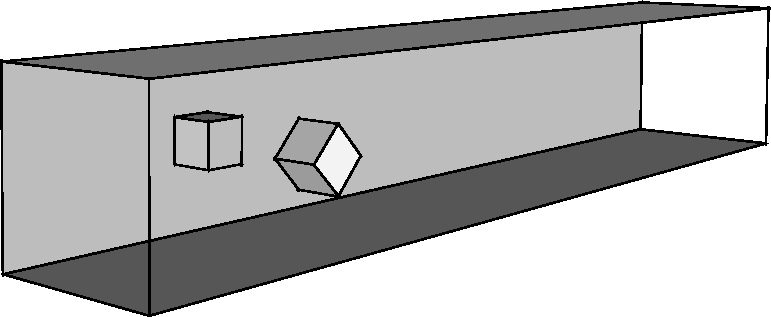
\includegraphics{./img/channel3d.pdf}
  \caption{Sketch of the channel flow problem domain}
  \label{fig:sketch}
\end{figure}

This case exercises all of the previously introduced boundary conditions for flow problems, including the treatment of non-matching block boundaries. For the velocities at the inflow boundary, the parabolic distribution
\begin{displaymath}
  \vec{u}(x_1,x_2,x_3) 
  =
\left[
  \begin{array}{ccc}
    u_1 \\
    u_2 \\
    u_3 
  \end{array}
\right]
  =
\left[
  \begin{array}{ccc}
    \frac{ 16 * 0.45 * x_2 * x_3 * \left( 0.41 - x_2 \right) * \left( 0.41 - x_3 \right)}{0.41^4}
    \\[0.9em]
    0 \\[0.3em]
    0 
  \end{array}
\right]
\end{displaymath}
was chosen. At the outlet a Dirichlet pressure boundary condition was used. All other boundaries used a no-slip solid non-moving wall boundary condition. All problem parameters were chosen to assure the flow problem resides in the regime of a non-turbulent stationary flow, for which the presented solver framework has been developed. Table \ref{tab:channel} lists the remaining material and geometrical characteristics of the test case. A study similar to section \ref{sec:speedup} was conducted to optimize the used amount of under-relaxation.

\begin{table}[h!]\centering
  \caption{Characteristic problem properties used in the channel flow test case}
\ra{1.3}
  \begin{tabular}{lcc}\toprule
    Property & Value & Unit \\
    \midrule
    \rowcolor{black!20} Density            & 1E-0 & $kg/m^3$  \\
    \rowcolor{black!00} Viscosity          & 1E-3 & $Ns/m^2$  \\
    \rowcolor{black!20} Height             & 0.41 & m         \\
    \rowcolor{black!00} Length             & 2.5  & m         \\
    \rowcolor{black!20} Side length cube   & 0.1  & m   \\
    \rowcolor{black!00} Under-relaxation u & 0.9  &    \\
    \rowcolor{black!20} Under-relaxation p & 0.1  &    \\
    \rowcolor{black!00} Relative tolerance & 1E-8      &
  \end{tabular}
  \label{tab:channel}
\end{table}

Using the data from table \ref{tab:channel} and the maximal inflow velocity of $0.45m/s$ the Reynolds number \(Re\) can be calculated as
\begin{displaymath}
  Re = \frac{\rho \operatorname{mean}(u_1) l}{\mu} = 20,
\end{displaymath}
where \(\operatorname{mean}(u_1) = 0.45*\frac{4}{9} m/s = 0.2 m/s\). This shows, that the flow resides in a laminar regime.

The present test case shows one advantage of the treatment of block boundaries, which has been introduced in section \ref{sec:blockboundaries}. Since no assumptions on the geometry of a neighboring block are necessary, the mesh for each block can be constructed independently which increases the flexibility of the meshing of geometries. Furthermore, because of the fully implicit handling of block boundaries, the number of used blocks does not negatively affect the convergence of the deployed linear solvers. Figure \ref{fig:channel1} shows the mesh at the left and right bounding walls. It is evident that this mesh leads to non-trivial transitions between the blocks. Figure \ref{fig:blocking} shows the domain decomposition into structured grid blocks around the two obstacles within the problem domain and emphasizes the need for accurate handling of non-matching block boundaries.

\begin{figure}
  \centering
  \begin{tikzpicture}[scale=1.15]
  
\draw ( 2.4410511  , 0.0771646) --   ( 2.2978751  , 0.0877825) --   ( 2.2500000  , 0.0000000) --   ( 2.4000000  , 0.0000000) -- cycle;
\draw ( 2.2978751  , 0.0877825) --   ( 2.1582372  , 0.1014927) --   ( 2.1000000  , 0.0000000) --   ( 2.2500000  , 0.0000000) -- cycle;
\draw ( 2.1582372  , 0.1014927) --   ( 2.0231447  , 0.1225456) --   ( 1.9500000  , 0.0000000) --   ( 2.1000000  , 0.0000000) -- cycle;
\draw ( 2.0231447  , 0.1225456) --   ( 1.8987309  , 0.1612305) --   ( 1.8000000  , 0.0000000) --   ( 1.9500000  , 0.0000000) -- cycle;
\draw ( 2.4785925  , 0.1570323) --   ( 2.3486426  , 0.1744382) --   ( 2.2978751  , 0.0877825) --   ( 2.4410511  , 0.0771646) -- cycle;
\draw ( 2.3486426  , 0.1744382) --   ( 2.2229947  , 0.1982127) --   ( 2.1582372  , 0.1014927) --   ( 2.2978751  , 0.0877825) -- cycle;
\draw ( 2.2229947  , 0.1982127) --   ( 2.1043777  , 0.2321397) --   ( 2.0231447  , 0.1225456) --   ( 2.1582372  , 0.1014927) -- cycle;
\draw ( 2.1043777  , 0.2321397) --   ( 1.9981788  , 0.2841135) --   ( 1.8987309  , 0.1612305) --   ( 2.0231447  , 0.1225456) -- cycle;
\draw ( 2.5193878  , 0.2358635) --   ( 2.4025145  , 0.2588656) --   ( 2.3486426  , 0.1744382) --   ( 2.4785925  , 0.1570323) -- cycle;
\draw ( 2.4025145  , 0.2588656) --   ( 2.2904549  , 0.2893299) --   ( 2.2229947  , 0.1982127) --   ( 2.3486426  , 0.1744382) -- cycle;
\draw ( 2.2904549  , 0.2893299) --   ( 2.1858209  , 0.3299841) --   ( 2.1043777  , 0.2321397) --   ( 2.2229947  , 0.1982127) -- cycle;
\draw ( 2.1858209  , 0.3299841) --   ( 2.0922327  , 0.3854525) --   ( 1.9981788  , 0.2841135) --   ( 2.1043777  , 0.2321397) -- cycle;
\draw ( 2.5629446  , 0.3121258) --   ( 2.4582318  , 0.3395666) --   ( 2.4025145  , 0.2588656) --   ( 2.5193878  , 0.2358635) -- cycle;
\draw ( 2.4582318  , 0.3395666) --   ( 2.3582441  , 0.3743399) --   ( 2.2904549  , 0.2893299) --   ( 2.4025145  , 0.2588656) -- cycle;
\draw ( 2.3582441  , 0.3743399) --   ( 2.2650172  , 0.4182042) --   ( 2.1858209  , 0.3299841) --   ( 2.2904549  , 0.2893299) -- cycle;
\draw ( 2.2650172  , 0.4182042) --   ( 2.1808601  , 0.4736248) --   ( 2.0922327  , 0.3854525) --   ( 2.1858209  , 0.3299841) -- cycle;
\draw ( 2.6087000  , 0.3851606) --   ( 2.5150604  , 0.4160143) --   ( 2.4582318  , 0.3395666) --   ( 2.5629446  , 0.3121258) -- cycle;
\draw ( 2.5150604  , 0.4160143) --   ( 2.4255008  , 0.4535462) --   ( 2.3582441  , 0.3743399) --   ( 2.4582318  , 0.3395666) -- cycle;
\draw ( 2.4255008  , 0.4535462) --   ( 2.3415843  , 0.4987738) --   ( 2.2650172  , 0.4182042) --   ( 2.3582441  , 0.3743399) -- cycle;
\draw ( 2.3415843  , 0.4987738) --   ( 2.2648661  , 0.5529431) --   ( 2.1808601  , 0.4736248) --   ( 2.2650172  , 0.4182042) -- cycle;
\draw ( 2.6567120  , 0.4544479) --   ( 2.5728744  , 0.4880104) --   ( 2.5150604  , 0.4160143) --   ( 2.6087000  , 0.3851606) -- cycle;
\draw ( 2.5728744  , 0.4880104) --   ( 2.4921166  , 0.5274035) --   ( 2.4255008  , 0.4535462) --   ( 2.5150604  , 0.4160143) -- cycle;
\draw ( 2.4921166  , 0.5274035) --   ( 2.4157681  , 0.5731614) --   ( 2.3415843  , 0.4987738) --   ( 2.4255008  , 0.4535462) -- cycle;
\draw ( 2.4157681  , 0.5731614) --   ( 2.3450141  , 0.6258438) --   ( 2.2648661  , 0.5529431) --   ( 2.3415843  , 0.4987738) -- cycle;
\draw ( 2.7075327  , 0.5195026) --   ( 2.6319115  , 0.5554404) --   ( 2.5728744  , 0.4880104) --   ( 2.6567120  , 0.4544479) -- cycle;
\draw ( 2.6319115  , 0.5554404) --   ( 2.5582983  , 0.5963474) --   ( 2.4921166  , 0.5274035) --   ( 2.5728744  , 0.4880104) -- cycle;
\draw ( 2.5582983  , 0.5963474) --   ( 2.4879680  , 0.6424297) --   ( 2.4157681  , 0.5731614) --   ( 2.4921166  , 0.5274035) -- cycle;
\draw ( 2.4879680  , 0.6424297) --   ( 2.4219291  , 0.6938747) --   ( 2.3450141  , 0.6258438) --   ( 2.4157681  , 0.5731614) -- cycle;
\draw ( 2.7617364  , 0.5798258) --   ( 2.6923791  , 0.6182278) --   ( 2.6319115  , 0.5554404) --   ( 2.7075327  , 0.5195026) -- cycle;
\draw ( 2.6923791  , 0.6182278) --   ( 2.6242447  , 0.6607658) --   ( 2.5582983  , 0.5963474) --   ( 2.6319115  , 0.5554404) -- cycle;
\draw ( 2.6242447  , 0.6607658) --   ( 2.5585495  , 0.7074200) --   ( 2.4879680  , 0.6424297) --   ( 2.5582983  , 0.5963474) -- cycle;
\draw ( 2.5585495  , 0.7074200) --   ( 2.4961467  , 0.7581525) --   ( 2.4219291  , 0.6938747) --   ( 2.4879680  , 0.6424297) -- cycle;
\draw ( 3.7027090  , 0.0882032) --   ( 3.5604041  , 0.0776380) --   ( 3.6000000  ,-0.0000000) --   ( 3.7500000  , 0.0000000) -- cycle;
\draw ( 3.8416319  , 0.1018258) --   ( 3.7027090  , 0.0882032) --   ( 3.7500000  , 0.0000000) --   ( 3.9000000  , 0.0000000) -- cycle;
\draw ( 3.9760265  , 0.1227268) --   ( 3.8416319  , 0.1018258) --   ( 3.9000000  , 0.0000000) --   ( 4.0500000  , 0.0000000) -- cycle;
\draw ( 4.0995984  , 0.1612508) --   ( 3.9760265  , 0.1227268) --   ( 4.0500000  , 0.0000000) --   ( 4.2000000  , 0.0000000) -- cycle;
\draw ( 3.6524222  , 0.1748348) --   ( 3.5236301  , 0.1575183) --   ( 3.5604041  , 0.0776380) --   ( 3.7027090  , 0.0882032) -- cycle;
\draw ( 3.7769967  , 0.1984361) --   ( 3.6524222  , 0.1748348) --   ( 3.7027090  , 0.0882032) --   ( 3.8416319  , 0.1018258) -- cycle;
\draw ( 3.8945735  , 0.2320968) --   ( 3.7769967  , 0.1984361) --   ( 3.8416319  , 0.1018258) --   ( 3.9760265  , 0.1227268) -- cycle;
\draw ( 3.9997895  , 0.2837283) --   ( 3.8945735  , 0.2320968) --   ( 3.9760265  , 0.1227268) --   ( 4.0995984  , 0.1612508) -- cycle;
\draw ( 3.5990043  , 0.2589718) --   ( 3.4833508  , 0.2361413) --   ( 3.5236301  , 0.1575183) --   ( 3.6524222  , 0.1748348) -- cycle;
\draw ( 3.7098930  , 0.2891563) --   ( 3.5990043  , 0.2589718) --   ( 3.6524222  , 0.1748348) --   ( 3.7769967  , 0.1984361) -- cycle;
\draw ( 3.8134147  , 0.3294179) --   ( 3.7098930  , 0.2891563) --   ( 3.7769967  , 0.1984361) --   ( 3.8945735  , 0.2320968) -- cycle;
\draw ( 3.9060300  , 0.3843687) --   ( 3.8134147  , 0.3294179) --   ( 3.8945735  , 0.2320968) --   ( 3.9997895  , 0.2837283) -- cycle;
\draw ( 3.5437142  , 0.3392276) --   ( 3.4401667  , 0.3120784) --   ( 3.4833508  , 0.2361413) --   ( 3.5990043  , 0.2589718) -- cycle;
\draw ( 3.6425931  , 0.3735933) --   ( 3.5437142  , 0.3392276) --   ( 3.5990043  , 0.2589718) --   ( 3.7098930  , 0.2891563) -- cycle;
\draw ( 3.7347913  , 0.4169439) --   ( 3.6425931  , 0.3735933) --   ( 3.7098930  , 0.2891563) --   ( 3.8134147  , 0.3294179) -- cycle;
\draw ( 3.8180396  , 0.4717281) --   ( 3.7347913  , 0.4169439) --   ( 3.8134147  , 0.3294179) --   ( 3.9060300  , 0.3843687) -- cycle;
\draw ( 3.4872404  , 0.4151492) --   ( 3.3946407  , 0.3847397) --   ( 3.4401667  , 0.3120784) --   ( 3.5437142  , 0.3392276) -- cycle;
\draw ( 3.5758491  , 0.4521369) --   ( 3.4872404  , 0.4151492) --   ( 3.5437142  , 0.3392276) --   ( 3.6425931  , 0.3735933) -- cycle;
\draw ( 3.6589100  , 0.4967588) --   ( 3.5758491  , 0.4521369) --   ( 3.6425931  , 0.3735933) --   ( 3.7347913  , 0.4169439) -- cycle;
\draw ( 3.7348295  , 0.5502627) --   ( 3.6589100  , 0.4967588) --   ( 3.7347913  , 0.4169439) --   ( 3.8180396  , 0.4717281) -- cycle;
\draw ( 3.4296643  , 0.4865880) --   ( 3.3467080  , 0.4536286) --   ( 3.3946407  , 0.3847397) --   ( 3.4872404  , 0.4151492) -- cycle;
\draw ( 3.5096804  , 0.5253198) --   ( 3.4296643  , 0.4865880) --   ( 3.4872404  , 0.4151492) --   ( 3.5758491  , 0.4521369) -- cycle;
\draw ( 3.5853911  , 0.5704422) --   ( 3.5096804  , 0.5253198) --   ( 3.5758491  , 0.4521369) --   ( 3.6589100  , 0.4967588) -- cycle;
\draw ( 3.6554930  , 0.6225447) --   ( 3.5853911  , 0.5704422) --   ( 3.6589100  , 0.4967588) --   ( 3.7348295  , 0.5502627) -- cycle;
\draw ( 3.3707011  , 0.5535075) --   ( 3.2958106  , 0.5183009) --   ( 3.3467080  , 0.4536286) --   ( 3.4296643  , 0.4865880) -- cycle;
\draw ( 3.4437812  , 0.5937128) --   ( 3.3707011  , 0.5535075) --   ( 3.4296643  , 0.4865880) --   ( 3.5096804  , 0.5253198) -- cycle;
\draw ( 3.5136798  , 0.6392343) --   ( 3.4437812  , 0.5937128) --   ( 3.5096804  , 0.5253198) --   ( 3.5853911  , 0.5704422) -- cycle;
\draw ( 3.5792181  , 0.6903026) --   ( 3.5136798  , 0.6392343) --   ( 3.5853911  , 0.5704422) --   ( 3.6554930  , 0.6225447) -- cycle;
\draw ( 3.3100159  , 0.6160617) --   ( 3.2413236  , 0.5783969) --   ( 3.2958106  , 0.5183009) --   ( 3.3707011  , 0.5535075) -- cycle;
\draw ( 3.3777424  , 0.6580067) --   ( 3.3100159  , 0.6160617) --   ( 3.3707011  , 0.5535075) --   ( 3.4437812  , 0.5937128) -- cycle;
\draw ( 3.4431259  , 0.7043051) --   ( 3.3777424  , 0.6580067) --   ( 3.4437812  , 0.5937128) --   ( 3.5136798  , 0.6392343) -- cycle;
\draw ( 3.5051402  , 0.7549144) --   ( 3.4431259  , 0.7043051) --   ( 3.5136798  , 0.6392343) --   ( 3.5792181  , 0.6903026) -- cycle;
\draw ( 3.5093076  , 1.7979432) --   ( 3.4374242  , 1.7292538) --   ( 3.4986694  , 1.6787236) --   ( 3.5742684  , 1.7469561) -- cycle;
\draw ( 3.5819977  , 1.8702705) --   ( 3.5093076  , 1.7979432) --   ( 3.5742684  , 1.7469561) --   ( 3.6516388  , 1.8182280) -- cycle;
\draw ( 3.6562954  , 1.9474207) --   ( 3.5819977  , 1.8702705) --   ( 3.6516388  , 1.8182280) --   ( 3.7318298  , 1.8939409) -- cycle;
\draw ( 3.7328205  , 2.0306117) --   ( 3.6562954  , 1.9474207) --   ( 3.7318298  , 1.8939409) --   ( 3.8157302  , 1.9758151) -- cycle;
\draw ( 3.8119837  , 2.1213915) --   ( 3.7328205  , 2.0306117) --   ( 3.8157302  , 1.9758151) --   ( 3.9042944  , 2.0664029) -- cycle;
\draw ( 3.8936206  , 2.2218383) --   ( 3.8119837  , 2.1213915) --   ( 3.9042944  , 2.0664029) --   ( 3.9985629  , 2.1701639) -- cycle;
\draw ( 3.9755360  , 2.3342275) --   ( 3.8936206  , 2.2218383) --   ( 3.9985629  , 2.1701639) --   ( 4.0989101  , 2.2956967) -- cycle;
\draw ( 4.0500000  , 2.4600000) --   ( 3.9755360  , 2.3342275) --   ( 4.0989101  , 2.2956967) --   ( 4.2000000  , 2.4600000) -- cycle;
\draw ( 3.4401493  , 1.8434772) --   ( 3.3730714  , 1.7754412) --   ( 3.4374242  , 1.7292538) --   ( 3.5093076  , 1.7979432) -- cycle;
\draw ( 3.5068506  , 1.9154535) --   ( 3.4401493  , 1.8434772) --   ( 3.5093076  , 1.7979432) --   ( 3.5819977  , 1.8702705) -- cycle;
\draw ( 3.5736784  , 1.9921138) --   ( 3.5068506  , 1.9154535) --   ( 3.5819977  , 1.8702705) --   ( 3.6562954  , 1.9474207) -- cycle;
\draw ( 3.6409784  , 2.0740231) --   ( 3.5736784  , 1.9921138) --   ( 3.6562954  , 1.9474207) --   ( 3.7328205  , 2.0306117) -- cycle;
\draw ( 3.7087493  , 2.1616967) --   ( 3.6409784  , 2.0740231) --   ( 3.7328205  , 2.0306117) --   ( 3.8119837  , 2.1213915) -- cycle;
\draw ( 3.7762586  , 2.2555178) --   ( 3.7087493  , 2.1616967) --   ( 3.8119837  , 2.1213915) --   ( 3.8936206  , 2.2218383) -- cycle;
\draw ( 3.8412658  , 2.3551247) --   ( 3.7762586  , 2.2555178) --   ( 3.8936206  , 2.2218383) --   ( 3.9755360  , 2.3342275) -- cycle;
\draw ( 3.9000000  , 2.4600000) --   ( 3.8412658  , 2.3551247) --   ( 3.9755360  , 2.3342275) --   ( 4.0500000  , 2.4600000) -- cycle;
\draw ( 3.3678722  , 1.8838299) --   ( 3.3064811  , 1.8173985) --   ( 3.3730714  , 1.7754412) --   ( 3.4401493  , 1.8434772) -- cycle;
\draw ( 3.4274277  , 1.9543649) --   ( 3.3678722  , 1.8838299) --   ( 3.4401493  , 1.8434772) --   ( 3.5068506  , 1.9154535) -- cycle;
\draw ( 3.4855184  , 2.0292613) --   ( 3.4274277  , 1.9543649) --   ( 3.5068506  , 1.9154535) --   ( 3.5736784  , 1.9921138) -- cycle;
\draw ( 3.5424395  , 2.1085124) --   ( 3.4855184  , 2.0292613) --   ( 3.5736784  , 1.9921138) --   ( 3.6409784  , 2.0740231) -- cycle;
\draw ( 3.5981111  , 2.1919726) --   ( 3.5424395  , 2.1085124) --   ( 3.6409784  , 2.0740231) --   ( 3.7087493  , 2.1616967) -- cycle;
\draw ( 3.6518478  , 2.2791833) --   ( 3.5981111  , 2.1919726) --   ( 3.7087493  , 2.1616967) --   ( 3.7762586  , 2.2555178) -- cycle;
\draw ( 3.7024201  , 2.3687889) --   ( 3.6518478  , 2.2791833) --   ( 3.7762586  , 2.2555178) --   ( 3.8412658  , 2.3551247) -- cycle;
\draw ( 3.7500000  , 2.4600000) --   ( 3.7024201  , 2.3687889) --   ( 3.8412658  , 2.3551247) --   ( 3.9000000  , 2.4600000) -- cycle;
\draw ( 3.2937372  , 1.9194038) --   ( 3.2388450  , 1.8554440) --   ( 3.3064811  , 1.8173985) --   ( 3.3678722  , 1.8838299) -- cycle;
\draw ( 3.3450321  , 1.9876378) --   ( 3.2937372  , 1.9194038) --   ( 3.3678722  , 1.8838299) --   ( 3.4274277  , 1.9543649) -- cycle;
\draw ( 3.3933374  , 2.0599175) --   ( 3.3450321  , 1.9876378) --   ( 3.4274277  , 1.9543649) --   ( 3.4855184  , 2.0292613) -- cycle;
\draw ( 3.4392001  , 2.1358427) --   ( 3.3933374  , 2.0599175) --   ( 3.4855184  , 2.0292613) --   ( 3.5424395  , 2.1085124) -- cycle;
\draw ( 3.4826751  , 2.2149410) --   ( 3.4392001  , 2.1358427) --   ( 3.5424395  , 2.1085124) --   ( 3.5981111  , 2.1919726) -- cycle;
\draw ( 3.5231871  , 2.2966139) --   ( 3.4826751  , 2.2149410) --   ( 3.5981111  , 2.1919726) --   ( 3.6518478  , 2.2791833) -- cycle;
\draw ( 3.5601518  , 2.3794784) --   ( 3.5231871  , 2.2966139) --   ( 3.6518478  , 2.2791833) --   ( 3.7024201  , 2.3687889) -- cycle;
\draw ( 3.6000000  , 2.4600000) --   ( 3.5601518  , 2.3794784) --   ( 3.7024201  , 2.3687889) --   ( 3.7500000  , 2.4600000) -- cycle;
\draw ( 2.2982795  , 2.3692240) --   ( 2.4414107  , 2.3799662) --   ( 2.4000000  , 2.4600000) --   ( 2.2500000  , 2.4600000) -- cycle;
\draw ( 2.1587283  , 2.3554724) --   ( 2.2982795  , 2.3692240) --   ( 2.2500000  , 2.4600000) --   ( 2.1000000  , 2.4600000) -- cycle;
\draw ( 2.0237713  , 2.3344149) --   ( 2.1587283  , 2.3554724) --   ( 2.1000000  , 2.4600000) --   ( 1.9500000  , 2.4600000) -- cycle;
\draw ( 1.8996067  , 2.2956867) --   ( 2.0237713  , 2.3344149) --   ( 1.9500000  , 2.4600000) --   ( 1.8000000  , 2.4600000) -- cycle;
\draw ( 2.3494250  , 2.2795785) --   ( 2.4792104  , 2.2971033) --   ( 2.4414107  , 2.3799662) --   ( 2.2982795  , 2.3692240) -- cycle;
\draw ( 2.2239682  , 2.2557326) --   ( 2.3494250  , 2.2795785) --   ( 2.2982795  , 2.3692240) --   ( 2.1587283  , 2.3554724) -- cycle;
\draw ( 2.1055847  , 2.2217675) --   ( 2.2239682  , 2.2557326) --   ( 2.1587283  , 2.3554724) --   ( 2.0237713  , 2.3344149) -- cycle;
\draw ( 1.9996907  , 2.1697008) --   ( 2.1055847  , 2.2217675) --   ( 2.0237713  , 2.3344149) --   ( 1.8996067  , 2.2956867) -- cycle;
\draw ( 2.4036697  , 2.1920715) --   ( 2.5202688  , 2.2152188) --   ( 2.4792104  , 2.2971033) --   ( 2.3494250  , 2.2795785) -- cycle;
\draw ( 2.2919002  , 2.1615047) --   ( 2.4036697  , 2.1920715) --   ( 2.3494250  , 2.2795785) --   ( 2.2239682  , 2.2557326) -- cycle;
\draw ( 2.1875729  , 2.1207790) --   ( 2.2919002  , 2.1615047) --   ( 2.2239682  , 2.2557326) --   ( 2.1055847  , 2.2217675) -- cycle;
\draw ( 2.0943004  , 2.0652134) --   ( 2.1875729  , 2.1207790) --   ( 2.1055847  , 2.2217675) --   ( 1.9996907  , 2.1697008) -- cycle;
\draw ( 2.4597829  , 2.1081851) --   ( 2.5641229  , 2.1358119) --   ( 2.5202688  , 2.2152188) --   ( 2.4036697  , 2.1920715) -- cycle;
\draw ( 2.3601784  , 2.0732718) --   ( 2.4597829  , 2.1081851) --   ( 2.4036697  , 2.1920715) --   ( 2.2919002  , 2.1615047) -- cycle;
\draw ( 2.2673226  , 2.0293118) --   ( 2.3601784  , 2.0732718) --   ( 2.2919002  , 2.1615047) --   ( 2.1875729  , 2.1207790) -- cycle;
\draw ( 2.1834968  , 1.9738054) --   ( 2.2673226  , 2.0293118) --   ( 2.1875729  , 2.1207790) --   ( 2.0943004  , 2.0652134) -- cycle;
\draw ( 2.5170525  , 2.0284357) --   ( 2.6102096  , 2.0595397) --   ( 2.5641229  , 2.1358119) --   ( 2.4597829  , 2.1081851) -- cycle;
\draw ( 2.4279770  , 1.9907245) --   ( 2.5170525  , 2.0284357) --   ( 2.4597829  , 2.1081851) --   ( 2.3601784  , 2.0732718) -- cycle;
\draw ( 2.3445100  , 1.9453782) --   ( 2.4279770  , 1.9907245) --   ( 2.3601784  , 2.0732718) --   ( 2.2673226  , 2.0293118) -- cycle;
\draw ( 2.2681568  , 1.8911359) --   ( 2.3445100  , 1.9453782) --   ( 2.2673226  , 2.0293118) --   ( 2.1834968  , 1.9738054) -- cycle;
\draw ( 2.5753685  , 1.9529963) --   ( 2.6585854  , 1.9868824) --   ( 2.6102096  , 2.0595397) --   ( 2.5170525  , 2.0284357) -- cycle;
\draw ( 2.4952323  , 1.9133904) --   ( 2.5753685  , 1.9529963) --   ( 2.5170525  , 2.0284357) --   ( 2.4279770  , 1.9907245) -- cycle;
\draw ( 2.4194453  , 1.8675017) --   ( 2.4952323  , 1.9133904) --   ( 2.4279770  , 1.9907245) --   ( 2.3445100  , 1.9453782) -- cycle;
\draw ( 2.3491240  , 1.8147527) --   ( 2.4194453  , 1.8675017) --   ( 2.3445100  , 1.9453782) --   ( 2.2681568  , 1.8911359) -- cycle;
\draw ( 2.6349931  , 1.8819177) --   ( 2.7097960  , 1.9182531) --   ( 2.6585854  , 1.9868824) --   ( 2.5753685  , 1.9529963) -- cycle;
\draw ( 2.5622070  , 1.8408070) --   ( 2.6349931  , 1.8819177) --   ( 2.5753685  , 1.9529963) --   ( 2.4952323  , 1.9133904) -- cycle;
\draw ( 2.4926173  , 1.7946188) --   ( 2.5622070  , 1.8408070) --   ( 2.4952323  , 1.9133904) --   ( 2.4194453  , 1.8675017) -- cycle;
\draw ( 2.4271240  , 1.7431132) --   ( 2.4926173  , 1.7946188) --   ( 2.4194453  , 1.8675017) --   ( 2.3491240  , 1.8147527) -- cycle;
\draw ( 2.6961695  , 1.8151526) --   ( 2.7644274  , 1.8539756) --   ( 2.7097960  , 1.9182531) --   ( 2.6349931  , 1.8819177) -- cycle;
\draw ( 2.6291905  , 1.7725508) --   ( 2.6961695  , 1.8151526) --   ( 2.6349931  , 1.8819177) --   ( 2.5622070  , 1.8408070) -- cycle;
\draw ( 2.5645238  , 1.7259220) --   ( 2.6291905  , 1.7725508) --   ( 2.5622070  , 1.8408070) --   ( 2.4926173  , 1.7946188) -- cycle;
\draw ( 2.5028493  , 1.6751523) --   ( 2.5645238  , 1.7259220) --   ( 2.4926173  , 1.7946188) --   ( 2.4271240  , 1.7431132) -- cycle;
\draw (14.8505642  , 1.0784004) --   (15.0000000  , 1.0784004) --   (15.0000000  , 1.2300842) --   (14.8505568  , 1.2300842) -- cycle;
\draw (14.7011076  , 1.0783801) --   (14.8505642  , 1.0784004) --   (14.8505568  , 1.2300842) --   (14.7010936  , 1.2301040) -- cycle;
\draw (14.5516021  , 1.0783617) --   (14.7011076  , 1.0783801) --   (14.7010936  , 1.2301040) --   (14.5515822  , 1.2301183) -- cycle;
\draw (14.4020326  , 1.0783452) --   (14.5516021  , 1.0783617) --   (14.5515822  , 1.2301183) --   (14.4020081  , 1.2301276) -- cycle;
\draw (14.2523853  , 1.0783306) --   (14.4020326  , 1.0783452) --   (14.4020081  , 1.2301276) --   (14.2523569  , 1.2301328) -- cycle;
\draw (14.1026533  , 1.0783177) --   (14.2523853  , 1.0783306) --   (14.2523569  , 1.2301328) --   (14.1026223  , 1.2301344) -- cycle;
\draw (13.9528345  , 1.0783066) --   (14.1026533  , 1.0783177) --   (14.1026223  , 1.2301344) --   (13.9528014  , 1.2301329) -- cycle;
\draw (13.8029328  , 1.0782965) --   (13.9528345  , 1.0783066) --   (13.9528014  , 1.2301329) --   (13.8028986  , 1.2301291) -- cycle;
\draw (13.6529556  , 1.0782876) --   (13.8029328  , 1.0782965) --   (13.8028986  , 1.2301291) --   (13.6529205  , 1.2301232) -- cycle;
\draw (13.5029123  , 1.0782797) --   (13.6529556  , 1.0782876) --   (13.6529205  , 1.2301232) --   (13.5028770  , 1.2301158) -- cycle;
\draw (13.3528145  , 1.0782726) --   (13.5029123  , 1.0782797) --   (13.5028770  , 1.2301158) --   (13.3527789  , 1.2301071) -- cycle;
\draw (13.2026732  , 1.0782660) --   (13.3528145  , 1.0782726) --   (13.3527789  , 1.2301071) --   (13.2026379  , 1.2300976) -- cycle;
\draw (13.0524999  , 1.0782596) --   (13.2026732  , 1.0782660) --   (13.2026379  , 1.2300976) --   (13.0524643  , 1.2300875) -- cycle;
\draw (12.9023044  , 1.0782533) --   (13.0524999  , 1.0782596) --   (13.0524643  , 1.2300875) --   (12.9022690  , 1.2300771) -- cycle;
\draw (12.7520962  , 1.0782469) --   (12.9023044  , 1.0782533) --   (12.9022690  , 1.2300771) --   (12.7520604  , 1.2300666) -- cycle;
\draw (12.6018827  , 1.0782403) --   (12.7520962  , 1.0782469) --   (12.7520604  , 1.2300666) --   (12.6018470  , 1.2300560) -- cycle;
\draw (12.4516707  , 1.0782337) --   (12.6018827  , 1.0782403) --   (12.6018470  , 1.2300560) --   (12.4516344  , 1.2300455) -- cycle;
\draw (12.3014647  , 1.0782269) --   (12.4516707  , 1.0782337) --   (12.4516344  , 1.2300455) --   (12.3014281  , 1.2300351) -- cycle;
\draw (12.1512685  , 1.0782200) --   (12.3014647  , 1.0782269) --   (12.3014281  , 1.2300351) --   (12.1512312  , 1.2300250) -- cycle;
\draw (12.0010845  , 1.0782131) --   (12.1512685  , 1.0782200) --   (12.1512312  , 1.2300250) --   (12.0010468  , 1.2300152) -- cycle;
\draw (11.8509147  , 1.0782061) --   (12.0010845  , 1.0782131) --   (12.0010468  , 1.2300152) --   (11.8508760  , 1.2300058) -- cycle;
\draw (11.7007595  , 1.0781992) --   (11.8509147  , 1.0782061) --   (11.8508760  , 1.2300058) --   (11.7007204  , 1.2299966) -- cycle;
\draw (11.5506199  , 1.0781924) --   (11.7007595  , 1.0781992) --   (11.7007204  , 1.2299966) --   (11.5505798  , 1.2299880) -- cycle;
\draw (11.4004952  , 1.0781858) --   (11.5506199  , 1.0781924) --   (11.5505798  , 1.2299880) --   (11.4004547  , 1.2299797) -- cycle;
\draw (11.2503860  , 1.0781794) --   (11.4004952  , 1.0781858) --   (11.4004547  , 1.2299797) --   (11.2503443  , 1.2299720) -- cycle;
\draw (11.1002911  , 1.0781734) --   (11.2503860  , 1.0781794) --   (11.2503443  , 1.2299720) --   (11.1002491  , 1.2299646) -- cycle;
\draw (10.9502111  , 1.0781677) --   (11.1002911  , 1.0781734) --   (11.1002491  , 1.2299646) --   (10.9501680  , 1.2299578) -- cycle;
\draw (10.8001452  , 1.0781624) --   (10.9502111  , 1.0781677) --   (10.9501680  , 1.2299578) --   (10.8001017  , 1.2299515) -- cycle;
\draw (10.6500940  , 1.0781577) --   (10.8001452  , 1.0781624) --   (10.8001017  , 1.2299515) --   (10.6500495  , 1.2299456) -- cycle;
\draw (10.5000571  , 1.0781533) --   (10.6500940  , 1.0781577) --   (10.6500495  , 1.2299456) --   (10.5000124  , 1.2299404) -- cycle;
\draw (10.3500357  , 1.0781496) --   (10.5000571  , 1.0781533) --   (10.5000124  , 1.2299404) --   (10.3499900  , 1.2299355) -- cycle;
\draw (10.2000292  , 1.0781462) --   (10.3500357  , 1.0781496) --   (10.3499900  , 1.2299355) --   (10.1999835  , 1.2299314) -- cycle;
\draw (10.0500384  , 1.0781432) --   (10.2000292  , 1.0781462) --   (10.1999835  , 1.2299314) --   (10.0499923  , 1.2299276) -- cycle;
\draw ( 9.9000615  , 1.0781399) --   (10.0500384  , 1.0781432) --   (10.0499923  , 1.2299276) --   ( 9.9000163  , 1.2299245) -- cycle;
\draw ( 9.7501004  , 1.0781360) --   ( 9.9000615  , 1.0781399) --   ( 9.9000163  , 1.2299245) --   ( 9.7500555  , 1.2299216) -- cycle;
\draw ( 9.6001644  , 1.0781314) --   ( 9.7501004  , 1.0781360) --   ( 9.7500555  , 1.2299216) --   ( 9.6001198  , 1.2299201) -- cycle;
\draw ( 9.4502581  , 1.0781270) --   ( 9.6001644  , 1.0781314) --   ( 9.6001198  , 1.2299201) --   ( 9.4502134  , 1.2299197) -- cycle;
\draw ( 9.3003798  , 1.0781218) --   ( 9.4502581  , 1.0781270) --   ( 9.4502134  , 1.2299197) --   ( 9.3003374  , 1.2299196) -- cycle;
\draw ( 9.1505397  , 1.0781159) --   ( 9.3003798  , 1.0781218) --   ( 9.3003374  , 1.2299196) --   ( 9.1504976  , 1.2299199) -- cycle;
\draw ( 9.0007378  , 1.0781092) --   ( 9.1505397  , 1.0781159) --   ( 9.1504976  , 1.2299199) --   ( 9.0006986  , 1.2299201) -- cycle;
\draw ( 8.8509882  , 1.0781014) --   ( 9.0007378  , 1.0781092) --   ( 9.0006986  , 1.2299201) --   ( 8.8509499  , 1.2299209) -- cycle;
\draw ( 8.7012976  , 1.0780931) --   ( 8.8509882  , 1.0781014) --   ( 8.8509499  , 1.2299209) --   ( 8.7012622  , 1.2299217) -- cycle;
\draw ( 8.5516826  , 1.0780834) --   ( 8.7012976  , 1.0780931) --   ( 8.7012622  , 1.2299217) --   ( 8.5516492  , 1.2299233) -- cycle;
\draw ( 8.4021568  , 1.0780731) --   ( 8.5516826  , 1.0780834) --   ( 8.5516492  , 1.2299233) --   ( 8.4021267  , 1.2299254) -- cycle;
\draw ( 8.2527404  , 1.0780612) --   ( 8.4021568  , 1.0780731) --   ( 8.4021267  , 1.2299254) --   ( 8.2527136  , 1.2299284) -- cycle;
\draw ( 8.1034540  , 1.0780482) --   ( 8.2527404  , 1.0780612) --   ( 8.2527136  , 1.2299284) --   ( 8.1034316  , 1.2299320) -- cycle;
\draw ( 7.9543235  , 1.0780332) --   ( 8.1034540  , 1.0780482) --   ( 8.1034316  , 1.2299320) --   ( 7.9543059  , 1.2299367) -- cycle;
\draw ( 7.8053774  , 1.0780164) --   ( 7.9543235  , 1.0780332) --   ( 7.9543059  , 1.2299367) --   ( 7.8053660  , 1.2299422) -- cycle;
\draw ( 7.6566498  , 1.0779969) --   ( 7.8053774  , 1.0780164) --   ( 7.8053660  , 1.2299422) --   ( 7.6566450  , 1.2299487) -- cycle;
\draw ( 7.5081786  , 1.0779743) --   ( 7.6566498  , 1.0779969) --   ( 7.6566450  , 1.2299487) --   ( 7.5081823  , 1.2299561) -- cycle;
\draw ( 7.3600084  , 1.0779481) --   ( 7.5081786  , 1.0779743) --   ( 7.5081823  , 1.2299561) --   ( 7.3600212  , 1.2299642) -- cycle;
\draw ( 7.2121885  , 1.0779170) --   ( 7.3600084  , 1.0779481) --   ( 7.3600212  , 1.2299642) --   ( 7.2122127  , 1.2299732) -- cycle;
\draw ( 7.0647762  , 1.0778804) --   ( 7.2121885  , 1.0779170) --   ( 7.2122127  , 1.2299732) --   ( 7.0648132  , 1.2299823) -- cycle;
\draw ( 6.9178348  , 1.0778359) --   ( 7.0647762  , 1.0778804) --   ( 7.0648132  , 1.2299823) --   ( 6.9178877  , 1.2299919) -- cycle;
\draw ( 6.7714371  , 1.0777826) --   ( 6.9178348  , 1.0778359) --   ( 6.9178877  , 1.2299919) --   ( 6.7715076  , 1.2300007) -- cycle;
\draw ( 6.6256626  , 1.0777164) --   ( 6.7714371  , 1.0777826) --   ( 6.7715076  , 1.2300007) --   ( 6.6257556  , 1.2300089) -- cycle;
\draw ( 6.4806026  , 1.0776351) --   ( 6.6256626  , 1.0777164) --   ( 6.6257556  , 1.2300089) --   ( 6.4807219  , 1.2300146) -- cycle;
\draw ( 6.3363576  , 1.0775335) --   ( 6.4806026  , 1.0776351) --   ( 6.4807219  , 1.2300146) --   ( 6.3365098  , 1.2300175) -- cycle;
\draw ( 6.1930409  , 1.0774062) --   ( 6.3363576  , 1.0775335) --   ( 6.3365098  , 1.2300175) --   ( 6.1932346  , 1.2300155) -- cycle;
\draw ( 6.0507811  , 1.0772472) --   ( 6.1930409  , 1.0774062) --   ( 6.1932346  , 1.2300155) --   ( 6.0510270  , 1.2300065) -- cycle;
\draw ( 5.9097233  , 1.0770487) --   ( 6.0507811  , 1.0772472) --   ( 6.0510270  , 1.2300065) --   ( 5.9100379  , 1.2299884) -- cycle;
\draw ( 5.7700356  , 1.0768043) --   ( 5.9097233  , 1.0770487) --   ( 5.9100379  , 1.2299884) --   ( 5.7704400  , 1.2299572) -- cycle;
\draw ( 5.6319119  , 1.0765078) --   ( 5.7700356  , 1.0768043) --   ( 5.7704400  , 1.2299572) --   ( 5.6324352  , 1.2299095) -- cycle;
\draw ( 5.4955781  , 1.0761616) --   ( 5.6319119  , 1.0765078) --   ( 5.6324352  , 1.2299095) --   ( 5.4962611  , 1.2298396) -- cycle;
\draw ( 5.3613090  , 1.0757807) --   ( 5.4955781  , 1.0761616) --   ( 5.4962611  , 1.2298396) --   ( 5.3621974  , 1.2297417) -- cycle;
\draw ( 5.2294238  , 1.0754060) --   ( 5.3613090  , 1.0757807) --   ( 5.3621974  , 1.2297417) --   ( 5.2305846  , 1.2296079) -- cycle;
\draw ( 5.1002996  , 1.0751191) --   ( 5.2294238  , 1.0754060) --   ( 5.2305846  , 1.2296079) --   ( 5.1018035  , 1.2294293) -- cycle;
\draw ( 4.9743674  , 1.0750717) --   ( 5.1002996  , 1.0751191) --   ( 5.1018035  , 1.2294293) --   ( 4.9762845  , 1.2291953) -- cycle;
\draw ( 4.8520877  , 1.0755186) --   ( 4.9743674  , 1.0750717) --   ( 4.9762845  , 1.2291953) --   ( 4.8544742  , 1.2288937) -- cycle;
\draw ( 4.7338975  , 1.0768107) --   ( 4.8520877  , 1.0755186) --   ( 4.8544742  , 1.2288937) --   ( 4.7367773  , 1.2285104) -- cycle;
\draw ( 4.6201242  , 1.0794013) --   ( 4.7338975  , 1.0768107) --   ( 4.7367773  , 1.2285104) --   ( 4.6234613  , 1.2280306) -- cycle;
\draw ( 4.5108706  , 1.0837220) --   ( 4.6201242  , 1.0794013) --   ( 4.6234613  , 1.2280306) --   ( 4.5145809  , 1.2274374) -- cycle;
\draw (14.8505820  , 0.9264617) --   (15.0000000  , 0.9264617) --   (15.0000000  , 1.0784004) --   (14.8505642  , 1.0784004) -- cycle;
\draw (14.7011399  , 0.9264051) --   (14.8505820  , 0.9264617) --   (14.8505642  , 1.0784004) --   (14.7011076  , 1.0783801) -- cycle;
\draw (14.5516457  , 0.9263570) --   (14.7011399  , 0.9264051) --   (14.7011076  , 1.0783801) --   (14.5516021  , 1.0783617) -- cycle;
\draw (14.4020840  , 0.9263170) --   (14.5516457  , 0.9263570) --   (14.5516021  , 1.0783617) --   (14.4020326  , 1.0783452) -- cycle;
\draw (14.2524413  , 0.9262841) --   (14.4020840  , 0.9263170) --   (14.4020326  , 1.0783452) --   (14.2523853  , 1.0783306) -- cycle;
\draw (14.1027112  , 0.9262580) --   (14.2524413  , 0.9262841) --   (14.2523853  , 1.0783306) --   (14.1026533  , 1.0783177) -- cycle;
\draw (13.9528920  , 0.9262377) --   (14.1027112  , 0.9262580) --   (14.1026533  , 1.0783177) --   (13.9528345  , 1.0783066) -- cycle;
\draw (13.8029884  , 0.9262223) --   (13.9528920  , 0.9262377) --   (13.9528345  , 1.0783066) --   (13.8029328  , 1.0782965) -- cycle;
\draw (13.6530078  , 0.9262107) --   (13.8029884  , 0.9262223) --   (13.8029328  , 1.0782965) --   (13.6529556  , 1.0782876) -- cycle;
\draw (13.5029608  , 0.9262025) --   (13.6530078  , 0.9262107) --   (13.6529556  , 1.0782876) --   (13.5029123  , 1.0782797) -- cycle;
\draw (13.3528588  , 0.9261970) --   (13.5029608  , 0.9262025) --   (13.5029123  , 1.0782797) --   (13.3528145  , 1.0782726) -- cycle;
\draw (13.2027139  , 0.9261933) --   (13.3528588  , 0.9261970) --   (13.3528145  , 1.0782726) --   (13.2026732  , 1.0782660) -- cycle;
\draw (13.0525370  , 0.9261906) --   (13.2027139  , 0.9261933) --   (13.2026732  , 1.0782660) --   (13.0524999  , 1.0782596) -- cycle;
\draw (12.9023390  , 0.9261883) --   (13.0525370  , 0.9261906) --   (13.0524999  , 1.0782596) --   (12.9023044  , 1.0782533) -- cycle;
\draw (12.7521286  , 0.9261860) --   (12.9023390  , 0.9261883) --   (12.9023044  , 1.0782533) --   (12.7520962  , 1.0782469) -- cycle;
\draw (12.6019140  , 0.9261835) --   (12.7521286  , 0.9261860) --   (12.7520962  , 1.0782469) --   (12.6018827  , 1.0782403) -- cycle;
\draw (12.4517010  , 0.9261808) --   (12.6019140  , 0.9261835) --   (12.6018827  , 1.0782403) --   (12.4516707  , 1.0782337) -- cycle;
\draw (12.3014949  , 0.9261777) --   (12.4517010  , 0.9261808) --   (12.4516707  , 1.0782337) --   (12.3014647  , 1.0782269) -- cycle;
\draw (12.1512988  , 0.9261744) --   (12.3014949  , 0.9261777) --   (12.3014647  , 1.0782269) --   (12.1512685  , 1.0782200) -- cycle;
\draw (12.0011156  , 0.9261706) --   (12.1512988  , 0.9261744) --   (12.1512685  , 1.0782200) --   (12.0010845  , 1.0782131) -- cycle;
\draw (11.8509464  , 0.9261667) --   (12.0011156  , 0.9261706) --   (12.0010845  , 1.0782131) --   (11.8509147  , 1.0782061) -- cycle;
\draw (11.7007926  , 0.9261626) --   (11.8509464  , 0.9261667) --   (11.8509147  , 1.0782061) --   (11.7007595  , 1.0781992) -- cycle;
\draw (11.5506539  , 0.9261584) --   (11.7007926  , 0.9261626) --   (11.7007595  , 1.0781992) --   (11.5506199  , 1.0781924) -- cycle;
\draw (11.4005308  , 0.9261542) --   (11.5506539  , 0.9261584) --   (11.5506199  , 1.0781924) --   (11.4004952  , 1.0781858) -- cycle;
\draw (11.2504225  , 0.9261502) --   (11.4005308  , 0.9261542) --   (11.4004952  , 1.0781858) --   (11.2503860  , 1.0781794) -- cycle;
\draw (11.1003292  , 0.9261463) --   (11.2504225  , 0.9261502) --   (11.2503860  , 1.0781794) --   (11.1002911  , 1.0781734) -- cycle;
\draw (10.9502500  , 0.9261426) --   (11.1003292  , 0.9261463) --   (11.1002911  , 1.0781734) --   (10.9502111  , 1.0781677) -- cycle;
\draw (10.8001854  , 0.9261391) --   (10.9502500  , 0.9261426) --   (10.9502111  , 1.0781677) --   (10.8001452  , 1.0781624) -- cycle;
\draw (10.6501347  , 0.9261357) --   (10.8001854  , 0.9261391) --   (10.8001452  , 1.0781624) --   (10.6500940  , 1.0781577) -- cycle;
\draw (10.5000987  , 0.9261324) --   (10.6501347  , 0.9261357) --   (10.6500940  , 1.0781577) --   (10.5000571  , 1.0781533) -- cycle;
\draw (10.3500769  , 0.9261287) --   (10.5000987  , 0.9261324) --   (10.5000571  , 1.0781533) --   (10.3500357  , 1.0781496) -- cycle;
\draw (10.2000703  , 0.9261246) --   (10.3500769  , 0.9261287) --   (10.3500357  , 1.0781496) --   (10.2000292  , 1.0781462) -- cycle;
\draw (10.0500783  , 0.9261195) --   (10.2000703  , 0.9261246) --   (10.2000292  , 1.0781462) --   (10.0500384  , 1.0781432) -- cycle;
\draw ( 9.9001006  , 0.9261140) --   (10.0500783  , 0.9261195) --   (10.0500384  , 1.0781432) --   ( 9.9000615  , 1.0781399) -- cycle;
\draw ( 9.7501377  , 0.9261085) --   ( 9.9001006  , 0.9261140) --   ( 9.9000615  , 1.0781399) --   ( 9.7501004  , 1.0781360) -- cycle;
\draw ( 9.6002003  , 0.9261031) --   ( 9.7501377  , 0.9261085) --   ( 9.7501004  , 1.0781360) --   ( 9.6001644  , 1.0781314) -- cycle;
\draw ( 9.4502905  , 0.9260964) --   ( 9.6002003  , 0.9261031) --   ( 9.6001644  , 1.0781314) --   ( 9.4502581  , 1.0781270) -- cycle;
\draw ( 9.3004089  , 0.9260883) --   ( 9.4502905  , 0.9260964) --   ( 9.4502581  , 1.0781270) --   ( 9.3003798  , 1.0781218) -- cycle;
\draw ( 9.1505640  , 0.9260786) --   ( 9.3004089  , 0.9260883) --   ( 9.3003798  , 1.0781218) --   ( 9.1505397  , 1.0781159) -- cycle;
\draw ( 9.0007570  , 0.9260670) --   ( 9.1505640  , 0.9260786) --   ( 9.1505397  , 1.0781159) --   ( 9.0007378  , 1.0781092) -- cycle;
\draw ( 8.8510009  , 0.9260540) --   ( 9.0007570  , 0.9260670) --   ( 9.0007378  , 1.0781092) --   ( 8.8509882  , 1.0781014) -- cycle;
\draw ( 8.7013030  , 0.9260387) --   ( 8.8510009  , 0.9260540) --   ( 8.8509882  , 1.0781014) --   ( 8.7012976  , 1.0780931) -- cycle;
\draw ( 8.5516792  , 0.9260218) --   ( 8.7013030  , 0.9260387) --   ( 8.7012976  , 1.0780931) --   ( 8.5516826  , 1.0780834) -- cycle;
\draw ( 8.4021428  , 0.9260023) --   ( 8.5516792  , 0.9260218) --   ( 8.5516826  , 1.0780834) --   ( 8.4021568  , 1.0780731) -- cycle;
\draw ( 8.2527140  , 0.9259803) --   ( 8.4021428  , 0.9260023) --   ( 8.4021568  , 1.0780731) --   ( 8.2527404  , 1.0780612) -- cycle;
\draw ( 8.1034127  , 0.9259550) --   ( 8.2527140  , 0.9259803) --   ( 8.2527404  , 1.0780612) --   ( 8.1034540  , 1.0780482) -- cycle;
\draw ( 7.9542646  , 0.9259262) --   ( 8.1034127  , 0.9259550) --   ( 8.1034540  , 1.0780482) --   ( 7.9543235  , 1.0780332) -- cycle;
\draw ( 7.8052982  , 0.9258928) --   ( 7.9542646  , 0.9259262) --   ( 7.9543235  , 1.0780332) --   ( 7.8053774  , 1.0780164) -- cycle;
\draw ( 7.6565462  , 0.9258545) --   ( 7.8052982  , 0.9258928) --   ( 7.8053774  , 1.0780164) --   ( 7.6566498  , 1.0779969) -- cycle;
\draw ( 7.5080472  , 0.9258101) --   ( 7.6565462  , 0.9258545) --   ( 7.6566498  , 1.0779969) --   ( 7.5081786  , 1.0779743) -- cycle;
\draw ( 7.3598439  , 0.9257584) --   ( 7.5080472  , 0.9258101) --   ( 7.5081786  , 1.0779743) --   ( 7.3600084  , 1.0779481) -- cycle;
\draw ( 7.2119861  , 0.9256983) --   ( 7.3598439  , 0.9257584) --   ( 7.3600084  , 1.0779481) --   ( 7.2121885  , 1.0779170) -- cycle;
\draw ( 7.0645289  , 0.9256272) --   ( 7.2119861  , 0.9256983) --   ( 7.2121885  , 1.0779170) --   ( 7.0647762  , 1.0778804) -- cycle;
\draw ( 6.9175357  , 0.9255436) --   ( 7.0645289  , 0.9256272) --   ( 7.0647762  , 1.0778804) --   ( 6.9178348  , 1.0778359) -- cycle;
\draw ( 6.7710761  , 0.9254430) --   ( 6.9175357  , 0.9255436) --   ( 6.9178348  , 1.0778359) --   ( 6.7714371  , 1.0777826) -- cycle;
\draw ( 6.6252291  , 0.9253226) --   ( 6.7710761  , 0.9254430) --   ( 6.7714371  , 1.0777826) --   ( 6.6256626  , 1.0777164) -- cycle;
\draw ( 6.4800813  , 0.9251756) --   ( 6.6252291  , 0.9253226) --   ( 6.6256626  , 1.0777164) --   ( 6.4806026  , 1.0776351) -- cycle;
\draw ( 6.3357296  , 0.9249957) --   ( 6.4800813  , 0.9251756) --   ( 6.4806026  , 1.0776351) --   ( 6.3363576  , 1.0775335) -- cycle;
\draw ( 6.1922813  , 0.9247745) --   ( 6.3357296  , 0.9249957) --   ( 6.3363576  , 1.0775335) --   ( 6.1930409  , 1.0774062) -- cycle;
\draw ( 6.0498554  , 0.9245011) --   ( 6.1922813  , 0.9247745) --   ( 6.1930409  , 1.0774062) --   ( 6.0507811  , 1.0772472) -- cycle;
\draw ( 5.9085857  , 0.9241654) --   ( 6.0498554  , 0.9245011) --   ( 6.0507811  , 1.0772472) --   ( 5.9097233  , 1.0770487) -- cycle;
\draw ( 5.7686223  , 0.9237558) --   ( 5.9085857  , 0.9241654) --   ( 5.9097233  , 1.0770487) --   ( 5.7700356  , 1.0768043) -- cycle;
\draw ( 5.6301353  , 0.9232672) --   ( 5.7686223  , 0.9237558) --   ( 5.7700356  , 1.0768043) --   ( 5.6319119  , 1.0765078) -- cycle;
\draw ( 5.4933262  , 0.9227042) --   ( 5.6301353  , 0.9232672) --   ( 5.6319119  , 1.0765078) --   ( 5.4955781  , 1.0761616) -- cycle;
\draw ( 5.3584312  , 0.9220990) --   ( 5.4933262  , 0.9227042) --   ( 5.4955781  , 1.0761616) --   ( 5.3613090  , 1.0757807) -- cycle;
\draw ( 5.2257292  , 0.9215292) --   ( 5.3584312  , 0.9220990) --   ( 5.3613090  , 1.0757807) --   ( 5.2294238  , 1.0754060) -- cycle;
\draw ( 5.0955715  , 0.9211535) --   ( 5.2257292  , 0.9215292) --   ( 5.2294238  , 1.0754060) --   ( 5.1002996  , 1.0751191) -- cycle;
\draw ( 4.9683768  , 0.9212748) --   ( 5.0955715  , 0.9211535) --   ( 5.1002996  , 1.0751191) --   ( 4.9743674  , 1.0750717) -- cycle;
\draw ( 4.8446420  , 0.9223821) --   ( 4.9683768  , 0.9212748) --   ( 4.9743674  , 1.0750717) --   ( 4.8520877  , 1.0755186) -- cycle;
\draw ( 4.7249067  , 0.9252274) --   ( 4.8446420  , 0.9223821) --   ( 4.8520877  , 1.0755186) --   ( 4.7338975  , 1.0768107) -- cycle;
\draw ( 4.6096778  , 0.9307827) --   ( 4.7249067  , 0.9252274) --   ( 4.7338975  , 1.0768107) --   ( 4.6201242  , 1.0794013) -- cycle;
\draw ( 4.4992371  , 0.9400463) --   ( 4.6096778  , 0.9307827) --   ( 4.6201242  , 1.0794013) --   ( 4.5108706  , 1.0837220) -- cycle;
\draw (14.8506117  , 0.7740384) --   (15.0000000  , 0.7740384) --   (15.0000000  , 0.9264617) --   (14.8505820  , 0.9264617) -- cycle;
\draw (14.7011932  , 0.7739542) --   (14.8506117  , 0.7740384) --   (14.8505820  , 0.9264617) --   (14.7011399  , 0.9264051) -- cycle;
\draw (14.5517169  , 0.7738830) --   (14.7011932  , 0.7739542) --   (14.7011399  , 0.9264051) --   (14.5516457  , 0.9263570) -- cycle;
\draw (14.4021667  , 0.7738246) --   (14.5517169  , 0.7738830) --   (14.5516457  , 0.9263570) --   (14.4020840  , 0.9263170) -- cycle;
\draw (14.2525297  , 0.7737773) --   (14.4021667  , 0.7738246) --   (14.4020840  , 0.9263170) --   (14.2524413  , 0.9262841) -- cycle;
\draw (14.1027999  , 0.7737404) --   (14.2525297  , 0.7737773) --   (14.2524413  , 0.9262841) --   (14.1027112  , 0.9262580) -- cycle;
\draw (13.9529773  , 0.7737132) --   (14.1027999  , 0.7737404) --   (14.1027112  , 0.9262580) --   (13.9528920  , 0.9262377) -- cycle;
\draw (13.8030672  , 0.7736937) --   (13.9529773  , 0.7737132) --   (13.9528920  , 0.9262377) --   (13.8029884  , 0.9262223) -- cycle;
\draw (13.6530787  , 0.7736804) --   (13.8030672  , 0.7736937) --   (13.8029884  , 0.9262223) --   (13.6530078  , 0.9262107) -- cycle;
\draw (13.5030226  , 0.7736723) --   (13.6530787  , 0.7736804) --   (13.6530078  , 0.9262107) --   (13.5029608  , 0.9262025) -- cycle;
\draw (13.3529119  , 0.7736684) --   (13.5030226  , 0.7736723) --   (13.5029608  , 0.9262025) --   (13.3528588  , 0.9261970) -- cycle;
\draw (13.2027587  , 0.7736673) --   (13.3529119  , 0.7736684) --   (13.3528588  , 0.9261970) --   (13.2027139  , 0.9261933) -- cycle;
\draw (13.0525749  , 0.7736678) --   (13.2027587  , 0.7736673) --   (13.2027139  , 0.9261933) --   (13.0525370  , 0.9261906) -- cycle;
\draw (12.9023709  , 0.7736690) --   (13.0525749  , 0.7736678) --   (13.0525370  , 0.9261906) --   (12.9023390  , 0.9261883) -- cycle;
\draw (12.7521563  , 0.7736702) --   (12.9023709  , 0.7736690) --   (12.9023390  , 0.9261883) --   (12.7521286  , 0.9261860) -- cycle;
\draw (12.6019384  , 0.7736712) --   (12.7521563  , 0.7736702) --   (12.7521286  , 0.9261860) --   (12.6019140  , 0.9261835) -- cycle;
\draw (12.4517237  , 0.7736718) --   (12.6019384  , 0.7736712) --   (12.6019140  , 0.9261835) --   (12.4517010  , 0.9261808) -- cycle;
\draw (12.3015165  , 0.7736719) --   (12.4517237  , 0.7736718) --   (12.4517010  , 0.9261808) --   (12.3014949  , 0.9261777) -- cycle;
\draw (12.1513205  , 0.7736714) --   (12.3015165  , 0.7736719) --   (12.3014949  , 0.9261777) --   (12.1512988  , 0.9261744) -- cycle;
\draw (12.0011377  , 0.7736705) --   (12.1513205  , 0.7736714) --   (12.1512988  , 0.9261744) --   (12.0011156  , 0.9261706) -- cycle;
\draw (11.8509698  , 0.7736690) --   (12.0011377  , 0.7736705) --   (12.0011156  , 0.9261706) --   (11.8509464  , 0.9261667) -- cycle;
\draw (11.7008172  , 0.7736672) --   (11.8509698  , 0.7736690) --   (11.8509464  , 0.9261667) --   (11.7007926  , 0.9261626) -- cycle;
\draw (11.5506804  , 0.7736651) --   (11.7008172  , 0.7736672) --   (11.7007926  , 0.9261626) --   (11.5506539  , 0.9261584) -- cycle;
\draw (11.4005589  , 0.7736629) --   (11.5506804  , 0.7736651) --   (11.5506539  , 0.9261584) --   (11.4005308  , 0.9261542) -- cycle;
\draw (11.2504527  , 0.7736606) --   (11.4005589  , 0.7736629) --   (11.4005308  , 0.9261542) --   (11.2504225  , 0.9261502) -- cycle;
\draw (11.1003608  , 0.7736583) --   (11.2504527  , 0.7736606) --   (11.2504225  , 0.9261502) --   (11.1003292  , 0.9261463) -- cycle;
\draw (10.9502835  , 0.7736561) --   (11.1003608  , 0.7736583) --   (11.1003292  , 0.9261463) --   (10.9502500  , 0.9261426) -- cycle;
\draw (10.8002199  , 0.7736538) --   (10.9502835  , 0.7736561) --   (10.9502500  , 0.9261426) --   (10.8001854  , 0.9261391) -- cycle;
\draw (10.6501703  , 0.7736517) --   (10.8002199  , 0.7736538) --   (10.8001854  , 0.9261391) --   (10.6501347  , 0.9261357) -- cycle;
\draw (10.5001343  , 0.7736494) --   (10.6501703  , 0.7736517) --   (10.6501347  , 0.9261357) --   (10.5000987  , 0.9261324) -- cycle;
\draw (10.3501125  , 0.7736469) --   (10.5001343  , 0.7736494) --   (10.5000987  , 0.9261324) --   (10.3500769  , 0.9261287) -- cycle;
\draw (10.2001044  , 0.7736437) --   (10.3501125  , 0.7736469) --   (10.3500769  , 0.9261287) --   (10.2000703  , 0.9261246) -- cycle;
\draw (10.0501109  , 0.7736397) --   (10.2001044  , 0.7736437) --   (10.2000703  , 0.9261246) --   (10.0500783  , 0.9261195) -- cycle;
\draw ( 9.9001311  , 0.7736347) --   (10.0501109  , 0.7736397) --   (10.0500783  , 0.9261195) --   ( 9.9001006  , 0.9261140) -- cycle;
\draw ( 9.7501673  , 0.7736297) --   ( 9.9001311  , 0.7736347) --   ( 9.9001006  , 0.9261140) --   ( 9.7501377  , 0.9261085) -- cycle;
\draw ( 9.6002261  , 0.7736242) --   ( 9.7501673  , 0.7736297) --   ( 9.7501377  , 0.9261085) --   ( 9.6002003  , 0.9261031) -- cycle;
\draw ( 9.4503115  , 0.7736171) --   ( 9.6002261  , 0.7736242) --   ( 9.6002003  , 0.9261031) --   ( 9.4502905  , 0.9260964) -- cycle;
\draw ( 9.3004241  , 0.7736082) --   ( 9.4503115  , 0.7736171) --   ( 9.4502905  , 0.9260964) --   ( 9.3004089  , 0.9260883) -- cycle;
\draw ( 9.1505715  , 0.7735972) --   ( 9.3004241  , 0.7736082) --   ( 9.3004089  , 0.9260883) --   ( 9.1505640  , 0.9260786) -- cycle;
\draw ( 9.0007560  , 0.7735843) --   ( 9.1505715  , 0.7735972) --   ( 9.1505640  , 0.9260786) --   ( 9.0007570  , 0.9260670) -- cycle;
\draw ( 8.8509895  , 0.7735691) --   ( 9.0007560  , 0.7735843) --   ( 9.0007570  , 0.9260670) --   ( 8.8510009  , 0.9260540) -- cycle;
\draw ( 8.7012791  , 0.7735518) --   ( 8.8509895  , 0.7735691) --   ( 8.8510009  , 0.9260540) --   ( 8.7013030  , 0.9260387) -- cycle;
\draw ( 8.5516405  , 0.7735317) --   ( 8.7012791  , 0.7735518) --   ( 8.7013030  , 0.9260387) --   ( 8.5516792  , 0.9260218) -- cycle;
\draw ( 8.4020864  , 0.7735090) --   ( 8.5516405  , 0.7735317) --   ( 8.5516792  , 0.9260218) --   ( 8.4021428  , 0.9260023) -- cycle;
\draw ( 8.2526364  , 0.7734826) --   ( 8.4020864  , 0.7735090) --   ( 8.4021428  , 0.9260023) --   ( 8.2527140  , 0.9259803) -- cycle;
\draw ( 8.1033100  , 0.7734524) --   ( 8.2526364  , 0.7734826) --   ( 8.2527140  , 0.9259803) --   ( 8.1034127  , 0.9259550) -- cycle;
\draw ( 7.9541326  , 0.7734173) --   ( 8.1033100  , 0.7734524) --   ( 8.1034127  , 0.9259550) --   ( 7.9542646  , 0.9259262) -- cycle;
\draw ( 7.8051311  , 0.7733769) --   ( 7.9541326  , 0.7734173) --   ( 7.9542646  , 0.9259262) --   ( 7.8052982  , 0.9258928) -- cycle;
\draw ( 7.6563390  , 0.7733300) --   ( 7.8051311  , 0.7733769) --   ( 7.8052982  , 0.9258928) --   ( 7.6565462  , 0.9258545) -- cycle;
\draw ( 7.5077922  , 0.7732756) --   ( 7.6563390  , 0.7733300) --   ( 7.6565462  , 0.9258545) --   ( 7.5080472  , 0.9258101) -- cycle;
\draw ( 7.3595342  , 0.7732125) --   ( 7.5077922  , 0.7732756) --   ( 7.5080472  , 0.9258101) --   ( 7.3598439  , 0.9257584) -- cycle;
\draw ( 7.2116121  , 0.7731385) --   ( 7.3595342  , 0.7732125) --   ( 7.3598439  , 0.9257584) --   ( 7.2119861  , 0.9256983) -- cycle;
\draw ( 7.0640808  , 0.7730521) --   ( 7.2116121  , 0.7731385) --   ( 7.2119861  , 0.9256983) --   ( 7.0645289  , 0.9256272) -- cycle;
\draw ( 6.9170006  , 0.7729494) --   ( 7.0640808  , 0.7730521) --   ( 7.0645289  , 0.9256272) --   ( 6.9175357  , 0.9255436) -- cycle;
\draw ( 6.7704399  , 0.7728277) --   ( 6.9170006  , 0.7729494) --   ( 6.9175357  , 0.9255436) --   ( 6.7710761  , 0.9254430) -- cycle;
\draw ( 6.6244732  , 0.7726807) --   ( 6.7704399  , 0.7728277) --   ( 6.7710761  , 0.9254430) --   ( 6.6252291  , 0.9253226) -- cycle;
\draw ( 6.4791833  , 0.7725030) --   ( 6.6244732  , 0.7726807) --   ( 6.6252291  , 0.9253226) --   ( 6.4800813  , 0.9251756) -- cycle;
\draw ( 6.3346602  , 0.7722857) --   ( 6.4791833  , 0.7725030) --   ( 6.4800813  , 0.9251756) --   ( 6.3357296  , 0.9249957) -- cycle;
\draw ( 6.1910022  , 0.7720182) --   ( 6.3346602  , 0.7722857) --   ( 6.3357296  , 0.9249957) --   ( 6.1922813  , 0.9247745) -- cycle;
\draw ( 6.0483153  , 0.7716888) --   ( 6.1910022  , 0.7720182) --   ( 6.1922813  , 0.9247745) --   ( 6.0498554  , 0.9245011) -- cycle;
\draw ( 5.9067148  , 0.7712831) --   ( 6.0483153  , 0.7716888) --   ( 6.0498554  , 0.9245011) --   ( 5.9085857  , 0.9241654) -- cycle;
\draw ( 5.7663234  , 0.7707888) --   ( 5.9067148  , 0.7712831) --   ( 5.9085857  , 0.9241654) --   ( 5.7686223  , 0.9237558) -- cycle;
\draw ( 5.6272780  , 0.7701978) --   ( 5.7663234  , 0.7707888) --   ( 5.7686223  , 0.9237558) --   ( 5.6301353  , 0.9232672) -- cycle;
\draw ( 5.4897327  , 0.7695174) --   ( 5.6272780  , 0.7701978) --   ( 5.6301353  , 0.9232672) --   ( 5.4933262  , 0.9227042) -- cycle;
\draw ( 5.3538590  , 0.7687838) --   ( 5.4897327  , 0.7695174) --   ( 5.4933262  , 0.9227042) --   ( 5.3584312  , 0.9220990) -- cycle;
\draw ( 5.2198752  , 0.7680938) --   ( 5.3538590  , 0.7687838) --   ( 5.3584312  , 0.9220990) --   ( 5.2257292  , 0.9215292) -- cycle;
\draw ( 5.0880565  , 0.7676625) --   ( 5.2198752  , 0.7680938) --   ( 5.2257292  , 0.9215292) --   ( 5.0955715  , 0.9211535) -- cycle;
\draw ( 4.9587804  , 0.7678840) --   ( 5.0880565  , 0.7676625) --   ( 5.0955715  , 0.9211535) --   ( 4.9683768  , 0.9212748) -- cycle;
\draw ( 4.8325608  , 0.7694646) --   ( 4.9587804  , 0.7678840) --   ( 4.9683768  , 0.9212748) --   ( 4.8446420  , 0.9223821) -- cycle;
\draw ( 4.7101010  , 0.7735453) --   ( 4.8325608  , 0.7694646) --   ( 4.8446420  , 0.9223821) --   ( 4.7249067  , 0.9252274) -- cycle;
\draw ( 4.5922211  , 0.7817608) --   ( 4.7101010  , 0.7735453) --   ( 4.7249067  , 0.9252274) --   ( 4.6096778  , 0.9307827) -- cycle;
\draw ( 4.4796366  , 0.7959899) --   ( 4.5922211  , 0.7817608) --   ( 4.6096778  , 0.9307827) --   ( 4.4992371  , 0.9400463) -- cycle;
\draw (14.8506544  , 0.6209325) --   (15.0000000  , 0.6209325) --   (15.0000000  , 0.7740384) --   (14.8506117  , 0.7740384) -- cycle;
\draw (14.7012700  , 0.6208331) --   (14.8506544  , 0.6209325) --   (14.8506117  , 0.7740384) --   (14.7011932  , 0.7739542) -- cycle;
\draw (14.5518193  , 0.6207490) --   (14.7012700  , 0.6208331) --   (14.7011932  , 0.7739542) --   (14.5517169  , 0.7738830) -- cycle;
\draw (14.4022848  , 0.6206798) --   (14.5518193  , 0.6207490) --   (14.5517169  , 0.7738830) --   (14.4021667  , 0.7738246) -- cycle;
\draw (14.2526545  , 0.6206240) --   (14.4022848  , 0.6206798) --   (14.4021667  , 0.7738246) --   (14.2525297  , 0.7737773) -- cycle;
\draw (14.1029235  , 0.6205810) --   (14.2526545  , 0.6206240) --   (14.2525297  , 0.7737773) --   (14.1027999  , 0.7737404) -- cycle;
\draw (13.9530935  , 0.6205498) --   (14.1029235  , 0.6205810) --   (14.1027999  , 0.7737404) --   (13.9529773  , 0.7737132) -- cycle;
\draw (13.8031720  , 0.6205282) --   (13.9530935  , 0.6205498) --   (13.9529773  , 0.7737132) --   (13.8030672  , 0.7736937) -- cycle;
\draw (13.6531695  , 0.6205143) --   (13.8031720  , 0.6205282) --   (13.8030672  , 0.7736937) --   (13.6530787  , 0.7736804) -- cycle;
\draw (13.5030989  , 0.6205069) --   (13.6531695  , 0.6205143) --   (13.6530787  , 0.7736804) --   (13.5030226  , 0.7736723) -- cycle;
\draw (13.3529736  , 0.6205045) --   (13.5030989  , 0.6205069) --   (13.5030226  , 0.7736723) --   (13.3529119  , 0.7736684) -- cycle;
\draw (13.2028074  , 0.6205055) --   (13.3529736  , 0.6205045) --   (13.3529119  , 0.7736684) --   (13.2027587  , 0.7736673) -- cycle;
\draw (13.0526122  , 0.6205084) --   (13.2028074  , 0.6205055) --   (13.2027587  , 0.7736673) --   (13.0525749  , 0.7736678) -- cycle;
\draw (12.9023993  , 0.6205119) --   (13.0526122  , 0.6205084) --   (13.0525749  , 0.7736678) --   (12.9023709  , 0.7736690) -- cycle;
\draw (12.7521774  , 0.6205156) --   (12.9023993  , 0.6205119) --   (12.9023709  , 0.7736690) --   (12.7521563  , 0.7736702) -- cycle;
\draw (12.6019546  , 0.6205190) --   (12.7521774  , 0.6205156) --   (12.7521563  , 0.7736702) --   (12.6019384  , 0.7736712) -- cycle;
\draw (12.4517365  , 0.6205218) --   (12.6019546  , 0.6205190) --   (12.6019384  , 0.7736712) --   (12.4517237  , 0.7736718) -- cycle;
\draw (12.3015277  , 0.6205239) --   (12.4517365  , 0.6205218) --   (12.4517237  , 0.7736718) --   (12.3015165  , 0.7736719) -- cycle;
\draw (12.1513311  , 0.6205253) --   (12.3015277  , 0.6205239) --   (12.3015165  , 0.7736719) --   (12.1513205  , 0.7736714) -- cycle;
\draw (12.0011490  , 0.6205260) --   (12.1513311  , 0.6205253) --   (12.1513205  , 0.7736714) --   (12.0011377  , 0.7736705) -- cycle;
\draw (11.8509823  , 0.6205261) --   (12.0011490  , 0.6205260) --   (12.0011377  , 0.7736705) --   (11.8509698  , 0.7736690) -- cycle;
\draw (11.7008317  , 0.6205257) --   (11.8509823  , 0.6205261) --   (11.8509698  , 0.7736690) --   (11.7008172  , 0.7736672) -- cycle;
\draw (11.5506969  , 0.6205250) --   (11.7008317  , 0.6205257) --   (11.7008172  , 0.7736672) --   (11.5506804  , 0.7736651) -- cycle;
\draw (11.4005779  , 0.6205239) --   (11.5506969  , 0.6205250) --   (11.5506804  , 0.7736651) --   (11.4005589  , 0.7736629) -- cycle;
\draw (11.2504738  , 0.6205227) --   (11.4005779  , 0.6205239) --   (11.4005589  , 0.7736629) --   (11.2504527  , 0.7736606) -- cycle;
\draw (11.1003845  , 0.6205215) --   (11.2504738  , 0.6205227) --   (11.2504527  , 0.7736606) --   (11.1003608  , 0.7736583) -- cycle;
\draw (10.9503089  , 0.6205203) --   (11.1003845  , 0.6205215) --   (11.1003608  , 0.7736583) --   (10.9502835  , 0.7736561) -- cycle;
\draw (10.8002472  , 0.6205191) --   (10.9503089  , 0.6205203) --   (10.9502835  , 0.7736561) --   (10.8002199  , 0.7736538) -- cycle;
\draw (10.6501986  , 0.6205180) --   (10.8002472  , 0.6205191) --   (10.8002199  , 0.7736538) --   (10.6501703  , 0.7736517) -- cycle;
\draw (10.5001634  , 0.6205170) --   (10.6501986  , 0.6205180) --   (10.6501703  , 0.7736517) --   (10.5001343  , 0.7736494) -- cycle;
\draw (10.3501411  , 0.6205159) --   (10.5001634  , 0.6205170) --   (10.5001343  , 0.7736494) --   (10.3501125  , 0.7736469) -- cycle;
\draw (10.2001322  , 0.6205146) --   (10.3501411  , 0.6205159) --   (10.3501125  , 0.7736469) --   (10.2001044  , 0.7736437) -- cycle;
\draw (10.0501363  , 0.6205128) --   (10.2001322  , 0.6205146) --   (10.2001044  , 0.7736437) --   (10.0501109  , 0.7736397) -- cycle;
\draw ( 9.9001544  , 0.6205105) --   (10.0501363  , 0.6205128) --   (10.0501109  , 0.7736397) --   ( 9.9001311  , 0.7736347) -- cycle;
\draw ( 9.7501876  , 0.6205076) --   ( 9.9001544  , 0.6205105) --   ( 9.9001311  , 0.7736347) --   ( 9.7501673  , 0.7736297) -- cycle;
\draw ( 9.6002417  , 0.6205037) --   ( 9.7501876  , 0.6205076) --   ( 9.7501673  , 0.7736297) --   ( 9.6002261  , 0.7736242) -- cycle;
\draw ( 9.4503202  , 0.6204975) --   ( 9.6002417  , 0.6205037) --   ( 9.6002261  , 0.7736242) --   ( 9.4503115  , 0.7736171) -- cycle;
\draw ( 9.3004255  , 0.6204893) --   ( 9.4503202  , 0.6204975) --   ( 9.4503115  , 0.7736171) --   ( 9.3004241  , 0.7736082) -- cycle;
\draw ( 9.1505624  , 0.6204790) --   ( 9.3004255  , 0.6204893) --   ( 9.3004241  , 0.7736082) --   ( 9.1505715  , 0.7735972) -- cycle;
\draw ( 9.0007359  , 0.6204666) --   ( 9.1505624  , 0.6204790) --   ( 9.1505715  , 0.7735972) --   ( 9.0007560  , 0.7735843) -- cycle;
\draw ( 8.8509548  , 0.6204524) --   ( 9.0007359  , 0.6204666) --   ( 9.0007560  , 0.7735843) --   ( 8.8509895  , 0.7735691) -- cycle;
\draw ( 8.7012279  , 0.6204357) --   ( 8.8509548  , 0.6204524) --   ( 8.8509895  , 0.7735691) --   ( 8.7012791  , 0.7735518) -- cycle;
\draw ( 8.5515684  , 0.6204169) --   ( 8.7012279  , 0.6204357) --   ( 8.7012791  , 0.7735518) --   ( 8.5516405  , 0.7735317) -- cycle;
\draw ( 8.4019903  , 0.6203950) --   ( 8.5515684  , 0.6204169) --   ( 8.5516405  , 0.7735317) --   ( 8.4020864  , 0.7735090) -- cycle;
\draw ( 8.2525109  , 0.6203699) --   ( 8.4019903  , 0.6203950) --   ( 8.4020864  , 0.7735090) --   ( 8.2526364  , 0.7734826) -- cycle;
\draw ( 8.1031502  , 0.6203405) --   ( 8.2525109  , 0.6203699) --   ( 8.2526364  , 0.7734826) --   ( 8.1033100  , 0.7734524) -- cycle;
\draw ( 7.9539318  , 0.6203066) --   ( 8.1031502  , 0.6203405) --   ( 8.1033100  , 0.7734524) --   ( 7.9541326  , 0.7734173) -- cycle;
\draw ( 7.8048829  , 0.6202670) --   ( 7.9539318  , 0.6203066) --   ( 7.9541326  , 0.7734173) --   ( 7.8051311  , 0.7733769) -- cycle;
\draw ( 7.6560345  , 0.6202211) --   ( 7.8048829  , 0.6202670) --   ( 7.8051311  , 0.7733769) --   ( 7.6563390  , 0.7733300) -- cycle;
\draw ( 7.5074232  , 0.6201678) --   ( 7.6560345  , 0.6202211) --   ( 7.6563390  , 0.7733300) --   ( 7.5077922  , 0.7732756) -- cycle;
\draw ( 7.3590893  , 0.6201056) --   ( 7.5074232  , 0.6201678) --   ( 7.5077922  , 0.7732756) --   ( 7.3595342  , 0.7732125) -- cycle;
\draw ( 7.2110802  , 0.6200333) --   ( 7.3590893  , 0.6201056) --   ( 7.3595342  , 0.7732125) --   ( 7.2116121  , 0.7731385) -- cycle;
\draw ( 7.0634476  , 0.6199481) --   ( 7.2110802  , 0.6200333) --   ( 7.2116121  , 0.7731385) --   ( 7.0640808  , 0.7730521) -- cycle;
\draw ( 6.9162508  , 0.6198479) --   ( 7.0634476  , 0.6199481) --   ( 7.0640808  , 0.7730521) --   ( 6.9170006  , 0.7729494) -- cycle;
\draw ( 6.7695542  , 0.6197281) --   ( 6.9162508  , 0.6198479) --   ( 6.9170006  , 0.7729494) --   ( 6.7704399  , 0.7728277) -- cycle;
\draw ( 6.6234293  , 0.6195847) --   ( 6.7695542  , 0.6197281) --   ( 6.7704399  , 0.7728277) --   ( 6.6244732  , 0.7726807) -- cycle;
\draw ( 6.4779534  , 0.6194104) --   ( 6.6234293  , 0.6195847) --   ( 6.6244732  , 0.7726807) --   ( 6.4791833  , 0.7725030) -- cycle;
\draw ( 6.3332095  , 0.6191975) --   ( 6.4779534  , 0.6194104) --   ( 6.4791833  , 0.7725030) --   ( 6.3346602  , 0.7722857) -- cycle;
\draw ( 6.1892849  , 0.6189351) --   ( 6.3332095  , 0.6191975) --   ( 6.3346602  , 0.7722857) --   ( 6.1910022  , 0.7720182) -- cycle;
\draw ( 6.0462715  , 0.6186108) --   ( 6.1892849  , 0.6189351) --   ( 6.1910022  , 0.7720182) --   ( 6.0483153  , 0.7716888) -- cycle;
\draw ( 5.9042608  , 0.6182104) --   ( 6.0462715  , 0.6186108) --   ( 6.0483153  , 0.7716888) --   ( 5.9067148  , 0.7712831) -- cycle;
\draw ( 5.7633469  , 0.6177199) --   ( 5.9042608  , 0.6182104) --   ( 5.9067148  , 0.7712831) --   ( 5.7663234  , 0.7707888) -- cycle;
\draw ( 5.6236219  , 0.6171309) --   ( 5.7633469  , 0.6177199) --   ( 5.7663234  , 0.7707888) --   ( 5.6272780  , 0.7701978) -- cycle;
\draw ( 5.4851747  , 0.6164467) --   ( 5.6236219  , 0.6171309) --   ( 5.6272780  , 0.7701978) --   ( 5.4897327  , 0.7695174) -- cycle;
\draw ( 5.3480998  , 0.6157023) --   ( 5.4851747  , 0.6164467) --   ( 5.4897327  , 0.7695174) --   ( 5.3538590  , 0.7687838) -- cycle;
\draw ( 5.2125039  , 0.6149962) --   ( 5.3480998  , 0.6157023) --   ( 5.3538590  , 0.7687838) --   ( 5.2198752  , 0.7680938) -- cycle;
\draw ( 5.0785377  , 0.6145418) --   ( 5.2125039  , 0.6149962) --   ( 5.2198752  , 0.7680938) --   ( 5.0880565  , 0.7676625) -- cycle;
\draw ( 4.9464453  , 0.6147766) --   ( 5.0785377  , 0.6145418) --   ( 5.0880565  , 0.7676625) --   ( 4.9587804  , 0.7678840) -- cycle;
\draw ( 4.8166825  , 0.6165246) --   ( 4.9464453  , 0.6147766) --   ( 4.9587804  , 0.7678840) --   ( 4.8325608  , 0.7694646) -- cycle;
\draw ( 4.6900590  , 0.6212617) --   ( 4.8166825  , 0.6165246) --   ( 4.8325608  , 0.7694646) --   ( 4.7101010  , 0.7735453) -- cycle;
\draw ( 4.5678990  , 0.6314435) --   ( 4.6900590  , 0.6212617) --   ( 4.7101010  , 0.7735453) --   ( 4.5922211  , 0.7817608) -- cycle;
\draw ( 4.4517954  , 0.6505127) --   ( 4.5678990  , 0.6314435) --   ( 4.5922211  , 0.7817608) --   ( 4.4796366  , 0.7959899) -- cycle;
\draw (14.8506388  , 1.8391565) --   (14.8505989  , 1.6860782) --   (15.0000000  , 1.6860782) --   (15.0000000  , 1.8391565) -- cycle;
\draw (14.7012333  , 1.8392832) --   (14.7011636  , 1.6861948) --   (14.8505989  , 1.6860782) --   (14.8506388  , 1.8391565) -- cycle;
\draw (14.5517596  , 1.8393859) --   (14.5516692  , 1.6862884) --   (14.7011636  , 1.6861948) --   (14.7012333  , 1.8392832) -- cycle;
\draw (14.4022016  , 1.8394661) --   (14.4021005  , 1.6863606) --   (14.5516692  , 1.6862884) --   (14.5517596  , 1.8393859) -- cycle;
\draw (14.2525477  , 1.8395269) --   (14.2524451  , 1.6864146) --   (14.4021005  , 1.6863606) --   (14.4022016  , 1.8394661) -- cycle;
\draw (14.1027943  , 1.8395696) --   (14.1026977  , 1.6864521) --   (14.2524451  , 1.6864146) --   (14.2525477  , 1.8395269) -- cycle;
\draw (13.9529430  , 1.8395963) --   (13.9528585  , 1.6864747) --   (14.1026977  , 1.6864521) --   (14.1027943  , 1.8395696) -- cycle;
\draw (13.8030018  , 1.8396099) --   (13.8029330  , 1.6864857) --   (13.9528585  , 1.6864747) --   (13.9529430  , 1.8395963) -- cycle;
\draw (13.6529813  , 1.8396131) --   (13.6529305  , 1.6864872) --   (13.8029330  , 1.6864857) --   (13.8030018  , 1.8396099) -- cycle;
\draw (13.5028946  , 1.8396077) --   (13.5028618  , 1.6864809) --   (13.6529305  , 1.6864872) --   (13.6529813  , 1.8396131) -- cycle;
\draw (13.3527551  , 1.8395955) --   (13.3527398  , 1.6864682) --   (13.5028618  , 1.6864809) --   (13.5028946  , 1.8396077) -- cycle;
\draw (13.2025765  , 1.8395786) --   (13.2025768  , 1.6864513) --   (13.3527398  , 1.6864682) --   (13.3527551  , 1.8395955) -- cycle;
\draw (13.0523705  , 1.8395592) --   (13.0523845  , 1.6864318) --   (13.2025768  , 1.6864513) --   (13.2025765  , 1.8395786) -- cycle;
\draw (12.9021482  , 1.8395384) --   (12.9021730  , 1.6864111) --   (13.0523845  , 1.6864318) --   (13.0523705  , 1.8395592) -- cycle;
\draw (12.7519182  , 1.8395173) --   (12.7519520  , 1.6863899) --   (12.9021730  , 1.6864111) --   (12.9021482  , 1.8395384) -- cycle;
\draw (12.6016884  , 1.8394964) --   (12.6017284  , 1.6863688) --   (12.7519520  , 1.6863899) --   (12.7519182  , 1.8395173) -- cycle;
\draw (12.4514642  , 1.8394760) --   (12.4515088  , 1.6863481) --   (12.6017284  , 1.6863688) --   (12.6016884  , 1.8394964) -- cycle;
\draw (12.3012500  , 1.8394565) --   (12.3012972  , 1.6863282) --   (12.4515088  , 1.6863481) --   (12.4514642  , 1.8394760) -- cycle;
\draw (12.1510485  , 1.8394380) --   (12.1510973  , 1.6863092) --   (12.3012972  , 1.6863282) --   (12.3012500  , 1.8394565) -- cycle;
\draw (12.0008619  , 1.8394206) --   (12.0009108  , 1.6862911) --   (12.1510973  , 1.6863092) --   (12.1510485  , 1.8394380) -- cycle;
\draw (11.8506909  , 1.8394042) --   (11.8507396  , 1.6862741) --   (12.0009108  , 1.6862911) --   (12.0008619  , 1.8394206) -- cycle;
\draw (11.7005363  , 1.8393888) --   (11.7005837  , 1.6862581) --   (11.8507396  , 1.6862741) --   (11.8506909  , 1.8394042) -- cycle;
\draw (11.5503975  , 1.8393746) --   (11.5504439  , 1.6862430) --   (11.7005837  , 1.6862581) --   (11.7005363  , 1.8393888) -- cycle;
\draw (11.4002747  , 1.8393612) --   (11.4003193  , 1.6862290) --   (11.5504439  , 1.6862430) --   (11.5503975  , 1.8393746) -- cycle;
\draw (11.2501670  , 1.8393488) --   (11.2502102  , 1.6862157) --   (11.4003193  , 1.6862290) --   (11.4002747  , 1.8393612) -- cycle;
\draw (11.1000742  , 1.8393370) --   (11.1001156  , 1.6862032) --   (11.2502102  , 1.6862157) --   (11.2501670  , 1.8393488) -- cycle;
\draw (10.9499957  , 1.8393259) --   (10.9500357  , 1.6861913) --   (11.1001156  , 1.6862032) --   (11.1000742  , 1.8393370) -- cycle;
\draw (10.7999314  , 1.8393149) --   (10.7999697  , 1.6861798) --   (10.9500357  , 1.6861913) --   (10.9499957  , 1.8393259) -- cycle;
\draw (10.6498808  , 1.8393037) --   (10.6499181  , 1.6861687) --   (10.7999697  , 1.6861798) --   (10.7999314  , 1.8393149) -- cycle;
\draw (10.4998440  , 1.8392918) --   (10.4998801  , 1.6861577) --   (10.6499181  , 1.6861687) --   (10.6498808  , 1.8393037) -- cycle;
\draw (10.3498200  , 1.8392787) --   (10.3498563  , 1.6861471) --   (10.4998801  , 1.6861577) --   (10.4998440  , 1.8392918) -- cycle;
\draw (10.1998091  , 1.8392646) --   (10.1998459  , 1.6861373) --   (10.3498563  , 1.6861471) --   (10.3498200  , 1.8392787) -- cycle;
\draw (10.0498095  , 1.8392500) --   (10.0498495  , 1.6861295) --   (10.1998459  , 1.6861373) --   (10.1998091  , 1.8392646) -- cycle;
\draw ( 9.8998211  , 1.8392371) --   ( 9.8998653  , 1.6861244) --   (10.0498495  , 1.6861295) --   (10.0498095  , 1.8392500) -- cycle;
\draw ( 9.7498442  , 1.8392278) --   ( 9.7498947  , 1.6861226) --   ( 9.8998653  , 1.6861244) --   ( 9.8998211  , 1.8392371) -- cycle;
\draw ( 9.5998891  , 1.8392242) --   ( 9.5999468  , 1.6861240) --   ( 9.7498947  , 1.6861226) --   ( 9.7498442  , 1.8392278) -- cycle;
\draw ( 9.4499646  , 1.8392267) --   ( 9.4500307  , 1.6861290) --   ( 9.5999468  , 1.6861240) --   ( 9.5998891  , 1.8392242) -- cycle;
\draw ( 9.3000687  , 1.8392334) --   ( 9.3001426  , 1.6861373) --   ( 9.4500307  , 1.6861290) --   ( 9.4499646  , 1.8392267) -- cycle;
\draw ( 9.1502047  , 1.8392438) --   ( 9.1502896  , 1.6861484) --   ( 9.3001426  , 1.6861373) --   ( 9.3000687  , 1.8392334) -- cycle;
\draw ( 9.0003789  , 1.8392565) --   ( 9.0004747  , 1.6861621) --   ( 9.1502896  , 1.6861484) --   ( 9.1502047  , 1.8392438) -- cycle;
\draw ( 8.8505954  , 1.8392713) --   ( 8.8507059  , 1.6861779) --   ( 9.0004747  , 1.6861621) --   ( 9.0003789  , 1.8392565) -- cycle;
\draw ( 8.7008668  , 1.8392882) --   ( 8.7009942  , 1.6861966) --   ( 8.8507059  , 1.6861779) --   ( 8.8505954  , 1.8392713) -- cycle;
\draw ( 8.5512025  , 1.8393081) --   ( 8.5513511  , 1.6862183) --   ( 8.7009942  , 1.6861966) --   ( 8.7008668  , 1.8392882) -- cycle;
\draw ( 8.4016193  , 1.8393312) --   ( 8.4017932  , 1.6862441) --   ( 8.5513511  , 1.6862183) --   ( 8.5512025  , 1.8393081) -- cycle;
\draw ( 8.2521328  , 1.8393589) --   ( 8.2523371  , 1.6862742) --   ( 8.4017932  , 1.6862441) --   ( 8.4016193  , 1.8393312) -- cycle;
\draw ( 8.1027644  , 1.8393915) --   ( 8.1030047  , 1.6863101) --   ( 8.2523371  , 1.6862742) --   ( 8.2521328  , 1.8393589) -- cycle;
\draw ( 7.9535364  , 1.8394303) --   ( 7.9538195  , 1.6863521) --   ( 8.1030047  , 1.6863101) --   ( 8.1027644  , 1.8393915) -- cycle;
\draw ( 7.8044769  , 1.8394760) --   ( 7.8048097  , 1.6864015) --   ( 7.9538195  , 1.6863521) --   ( 7.9535364  , 1.8394303) -- cycle;
\draw ( 7.6556161  , 1.8395296) --   ( 7.6560076  , 1.6864592) --   ( 7.8048097  , 1.6864015) --   ( 7.8044769  , 1.8394760) -- cycle;
\draw ( 7.5069906  , 1.8395925) --   ( 7.5074498  , 1.6865261) --   ( 7.6560076  , 1.6864592) --   ( 7.6556161  , 1.8395296) -- cycle;
\draw ( 7.3586405  , 1.8396657) --   ( 7.3591788  , 1.6866040) --   ( 7.5074498  , 1.6865261) --   ( 7.5069906  , 1.8395925) -- cycle;
\draw ( 7.2106127  , 1.8397511) --   ( 7.2112421  , 1.6866941) --   ( 7.3591788  , 1.6866040) --   ( 7.3586405  , 1.8396657) -- cycle;
\draw ( 7.0629589  , 1.8398503) --   ( 7.0636940  , 1.6867986) --   ( 7.2112421  , 1.6866941) --   ( 7.2106127  , 1.8397511) -- cycle;
\draw ( 6.9157377  , 1.8399661) --   ( 6.9165948  , 1.6869199) --   ( 7.0636940  , 1.6867986) --   ( 7.0629589  , 1.8398503) -- cycle;
\draw ( 6.7690136  , 1.8401016) --   ( 6.7700123  , 1.6870612) --   ( 6.9165948  , 1.6869199) --   ( 6.9157377  , 1.8399661) -- cycle;
\draw ( 6.6228574  , 1.8402610) --   ( 6.6240210  , 1.6872265) --   ( 6.7700123  , 1.6870612) --   ( 6.7690136  , 1.8401016) -- cycle;
\draw ( 6.4773458  , 1.8404495) --   ( 6.4787034  , 1.6874212) --   ( 6.6240210  , 1.6872265) --   ( 6.6228574  , 1.8402610) -- cycle;
\draw ( 6.3325616  , 1.8406745) --   ( 6.3341486  , 1.6876514) --   ( 6.4787034  , 1.6874212) --   ( 6.4773458  , 1.8404495) -- cycle;
\draw ( 6.1885913  , 1.8409439) --   ( 6.1904552  , 1.6879259) --   ( 6.3341486  , 1.6876514) --   ( 6.3325616  , 1.8406745) -- cycle;
\draw ( 6.0455269  , 1.8412682) --   ( 6.0477283  , 1.6882528) --   ( 6.1904552  , 1.6879259) --   ( 6.1885913  , 1.8409439) -- cycle;
\draw ( 5.9034592  , 1.8416577) --   ( 5.9060834  , 1.6886424) --   ( 6.0477283  , 1.6882528) --   ( 6.0455269  , 1.8412682) -- cycle;
\draw ( 5.7624823  , 1.8421220) --   ( 5.7656425  , 1.6891016) --   ( 5.9060834  , 1.6886424) --   ( 5.9034592  , 1.8416577) -- cycle;
\draw ( 5.6226882  , 1.8426634) --   ( 5.6265427  , 1.6896311) --   ( 5.7656425  , 1.6891016) --   ( 5.7624823  , 1.8421220) -- cycle;
\draw ( 5.4841663  , 1.8432700) --   ( 5.4889383  , 1.6902151) --   ( 5.6265427  , 1.6896311) --   ( 5.6226882  , 1.8426634) -- cycle;
\draw ( 5.3470123  , 1.8438972) --   ( 5.3530007  , 1.6908049) --   ( 5.4889383  , 1.6902151) --   ( 5.4841663  , 1.8432700) -- cycle;
\draw ( 5.2113339  , 1.8444313) --   ( 5.2189496  , 1.6912900) --   ( 5.3530007  , 1.6908049) --   ( 5.3470123  , 1.8438972) -- cycle;
\draw ( 5.0772842  , 1.8446421) --   ( 5.0870602  , 1.6914353) --   ( 5.2189496  , 1.6912900) --   ( 5.2113339  , 1.8444313) -- cycle;
\draw ( 4.9451083  , 1.8440670) --   ( 4.9577110  , 1.6908250) --   ( 5.0870602  , 1.6914353) --   ( 5.0772842  , 1.8446421) -- cycle;
\draw ( 4.8152637  , 1.8418523) --   ( 4.8314160  , 1.6887234) --   ( 4.9577110  , 1.6908250) --   ( 4.9451083  , 1.8440670) -- cycle;
\draw ( 4.6885595  , 1.8364831) --   ( 4.7088793  , 1.6839562) --   ( 4.8314160  , 1.6887234) --   ( 4.8152637  , 1.8418523) -- cycle;
\draw ( 4.5663186  , 1.8254574) --   ( 4.5909229  , 1.6748480) --   ( 4.7088793  , 1.6839562) --   ( 4.6885595  , 1.8364831) -- cycle;
\draw ( 4.4501362  , 1.8052753) --   ( 4.4782703  , 1.6594704) --   ( 4.5909229  , 1.6748480) --   ( 4.5663186  , 1.8254574) -- cycle;
\draw (14.8505989  , 1.6860782) --   (14.8505729  , 1.5336807) --   (15.0000000  , 1.5336807) --   (15.0000000  , 1.6860782) -- cycle;
\draw (14.7011636  , 1.6861948) --   (14.7011190  , 1.5337735) --   (14.8505729  , 1.5336807) --   (14.8505989  , 1.6860782) -- cycle;
\draw (14.5516692  , 1.6862884) --   (14.5516121  , 1.5338471) --   (14.7011190  , 1.5337735) --   (14.7011636  , 1.6861948) -- cycle;
\draw (14.4021005  , 1.6863606) --   (14.4020378  , 1.5339032) --   (14.5516121  , 1.5338471) --   (14.5516692  , 1.6862884) -- cycle;
\draw (14.2524451  , 1.6864146) --   (14.2523824  , 1.5339445) --   (14.4020378  , 1.5339032) --   (14.4021005  , 1.6863606) -- cycle;
\draw (14.1026977  , 1.6864521) --   (14.1026403  , 1.5339723) --   (14.2523824  , 1.5339445) --   (14.2524451  , 1.6864146) -- cycle;
\draw (13.9528585  , 1.6864747) --   (13.9528096  , 1.5339885) --   (14.1026403  , 1.5339723) --   (14.1026977  , 1.6864521) -- cycle;
\draw (13.8029330  , 1.6864857) --   (13.8028954  , 1.5339954) --   (13.9528096  , 1.5339885) --   (13.9528585  , 1.6864747) -- cycle;
\draw (13.6529305  , 1.6864872) --   (13.6529052  , 1.5339949) --   (13.8028954  , 1.5339954) --   (13.8029330  , 1.6864857) -- cycle;
\draw (13.5028618  , 1.6864809) --   (13.5028495  , 1.5339881) --   (13.6529052  , 1.5339949) --   (13.6529305  , 1.6864872) -- cycle;
\draw (13.3527398  , 1.6864682) --   (13.3527397  , 1.5339761) --   (13.5028495  , 1.5339881) --   (13.5028618  , 1.6864809) -- cycle;
\draw (13.2025768  , 1.6864513) --   (13.2025880  , 1.5339608) --   (13.3527397  , 1.5339761) --   (13.3527398  , 1.6864682) -- cycle;
\draw (13.0523845  , 1.6864318) --   (13.0524052  , 1.5339434) --   (13.2025880  , 1.5339608) --   (13.2025768  , 1.6864513) -- cycle;
\draw (12.9021730  , 1.6864111) --   (12.9022020  , 1.5339250) --   (13.0524052  , 1.5339434) --   (13.0523845  , 1.6864318) -- cycle;
\draw (12.7519520  , 1.6863899) --   (12.7519870  , 1.5339062) --   (12.9022020  , 1.5339250) --   (12.9021730  , 1.6864111) -- cycle;
\draw (12.6017284  , 1.6863688) --   (12.6017685  , 1.5338874) --   (12.7519870  , 1.5339062) --   (12.7519520  , 1.6863899) -- cycle;
\draw (12.4515088  , 1.6863481) --   (12.4515521  , 1.5338690) --   (12.6017685  , 1.5338874) --   (12.6017284  , 1.6863688) -- cycle;
\draw (12.3012972  , 1.6863282) --   (12.3013429  , 1.5338513) --   (12.4515521  , 1.5338690) --   (12.4515088  , 1.6863481) -- cycle;
\draw (12.1510973  , 1.6863092) --   (12.1511440  , 1.5338343) --   (12.3013429  , 1.5338513) --   (12.3012972  , 1.6863282) -- cycle;
\draw (12.0009108  , 1.6862911) --   (12.0009583  , 1.5338182) --   (12.1511440  , 1.5338343) --   (12.1510973  , 1.6863092) -- cycle;
\draw (11.8507396  , 1.6862741) --   (11.8507867  , 1.5338030) --   (12.0009583  , 1.5338182) --   (12.0009108  , 1.6862911) -- cycle;
\draw (11.7005837  , 1.6862581) --   (11.7006306  , 1.5337886) --   (11.8507867  , 1.5338030) --   (11.8507396  , 1.6862741) -- cycle;
\draw (11.5504439  , 1.6862430) --   (11.5504898  , 1.5337752) --   (11.7006306  , 1.5337886) --   (11.7005837  , 1.6862581) -- cycle;
\draw (11.4003193  , 1.6862290) --   (11.4003646  , 1.5337626) --   (11.5504898  , 1.5337752) --   (11.5504439  , 1.6862430) -- cycle;
\draw (11.2502102  , 1.6862157) --   (11.2502543  , 1.5337508) --   (11.4003646  , 1.5337626) --   (11.4003193  , 1.6862290) -- cycle;
\draw (11.1001156  , 1.6862032) --   (11.1001590  , 1.5337396) --   (11.2502543  , 1.5337508) --   (11.2502102  , 1.6862157) -- cycle;
\draw (10.9500357  , 1.6861913) --   (10.9500780  , 1.5337291) --   (11.1001590  , 1.5337396) --   (11.1001156  , 1.6862032) -- cycle;
\draw (10.7999697  , 1.6861798) --   (10.8000116  , 1.5337191) --   (10.9500780  , 1.5337291) --   (10.9500357  , 1.6861913) -- cycle;
\draw (10.6499181  , 1.6861687) --   (10.6499592  , 1.5337096) --   (10.8000116  , 1.5337191) --   (10.7999697  , 1.6861798) -- cycle;
\draw (10.4998801  , 1.6861577) --   (10.4999215  , 1.5337008) --   (10.6499592  , 1.5337096) --   (10.6499181  , 1.6861687) -- cycle;
\draw (10.3498563  , 1.6861471) --   (10.3498981  , 1.5336925) --   (10.4999215  , 1.5337008) --   (10.4998801  , 1.6861577) -- cycle;
\draw (10.1998459  , 1.6861373) --   (10.1998899  , 1.5336858) --   (10.3498981  , 1.5336925) --   (10.3498563  , 1.6861471) -- cycle;
\draw (10.0498495  , 1.6861295) --   (10.0498962  , 1.5336808) --   (10.1998899  , 1.5336858) --   (10.1998459  , 1.6861373) -- cycle;
\draw ( 9.8998653  , 1.6861244) --   ( 9.8999166  , 1.5336785) --   (10.0498962  , 1.5336808) --   (10.0498495  , 1.6861295) -- cycle;
\draw ( 9.7498947  , 1.6861226) --   ( 9.7499500  , 1.5336793) --   ( 9.8999166  , 1.5336785) --   ( 9.8998653  , 1.6861244) -- cycle;
\draw ( 9.5999468  , 1.6861240) --   ( 9.6000073  , 1.5336827) --   ( 9.7499500  , 1.5336793) --   ( 9.7498947  , 1.6861226) -- cycle;
\draw ( 9.4500307  , 1.6861290) --   ( 9.4500962  , 1.5336880) --   ( 9.6000073  , 1.5336827) --   ( 9.5999468  , 1.6861240) -- cycle;
\draw ( 9.3001426  , 1.6861373) --   ( 9.3002152  , 1.5336960) --   ( 9.4500962  , 1.5336880) --   ( 9.4500307  , 1.6861290) -- cycle;
\draw ( 9.1502896  , 1.6861484) --   ( 9.1503689  , 1.5337062) --   ( 9.3002152  , 1.5336960) --   ( 9.3001426  , 1.6861373) -- cycle;
\draw ( 9.0004747  , 1.6861621) --   ( 9.0005633  , 1.5337181) --   ( 9.1503689  , 1.5337062) --   ( 9.1502896  , 1.6861484) -- cycle;
\draw ( 8.8507059  , 1.6861779) --   ( 8.8508047  , 1.5337326) --   ( 9.0005633  , 1.5337181) --   ( 9.0004747  , 1.6861621) -- cycle;
\draw ( 8.7009942  , 1.6861966) --   ( 8.7011063  , 1.5337491) --   ( 8.8508047  , 1.5337326) --   ( 8.8507059  , 1.6861779) -- cycle;
\draw ( 8.5513511  , 1.6862183) --   ( 8.5514789  , 1.5337690) --   ( 8.7011063  , 1.5337491) --   ( 8.7009942  , 1.6861966) -- cycle;
\draw ( 8.4017932  , 1.6862441) --   ( 8.4019402  , 1.5337920) --   ( 8.5514789  , 1.5337690) --   ( 8.5513511  , 1.6862183) -- cycle;
\draw ( 8.2523371  , 1.6862742) --   ( 8.2525068  , 1.5338194) --   ( 8.4019402  , 1.5337920) --   ( 8.4017932  , 1.6862441) -- cycle;
\draw ( 8.1030047  , 1.6863101) --   ( 8.1032015  , 1.5338514) --   ( 8.2525068  , 1.5338194) --   ( 8.2523371  , 1.6862742) -- cycle;
\draw ( 7.9538195  , 1.6863521) --   ( 7.9540479  , 1.5338890) --   ( 8.1032015  , 1.5338514) --   ( 8.1030047  , 1.6863101) -- cycle;
\draw ( 7.8048097  , 1.6864015) --   ( 7.8050758  , 1.5339328) --   ( 7.9540479  , 1.5338890) --   ( 7.9538195  , 1.6863521) -- cycle;
\draw ( 7.6560076  , 1.6864592) --   ( 7.6563170  , 1.5339837) --   ( 7.8050758  , 1.5339328) --   ( 7.8048097  , 1.6864015) -- cycle;
\draw ( 7.5074498  , 1.6865261) --   ( 7.5078104  , 1.5340426) --   ( 7.6563170  , 1.5339837) --   ( 7.6560076  , 1.6864592) -- cycle;
\draw ( 7.3591788  , 1.6866040) --   ( 7.3595983  , 1.5341105) --   ( 7.5078104  , 1.5340426) --   ( 7.5074498  , 1.6865261) -- cycle;
\draw ( 7.2112421  , 1.6866941) --   ( 7.2117304  , 1.5341889) --   ( 7.3595983  , 1.5341105) --   ( 7.3591788  , 1.6866040) -- cycle;
\draw ( 7.0636940  , 1.6867986) --   ( 7.0642618  , 1.5342789) --   ( 7.2117304  , 1.5341889) --   ( 7.2112421  , 1.6866941) -- cycle;
\draw ( 6.9165948  , 1.6869199) --   ( 6.9172555  , 1.5343830) --   ( 7.0642618  , 1.5342789) --   ( 7.0636940  , 1.6867986) -- cycle;
\draw ( 6.7700123  , 1.6870612) --   ( 6.7707811  , 1.5345032) --   ( 6.9172555  , 1.5343830) --   ( 6.9165948  , 1.6869199) -- cycle;
\draw ( 6.6240210  , 1.6872265) --   ( 6.6249174  , 1.5346428) --   ( 6.7707811  , 1.5345032) --   ( 6.7700123  , 1.6870612) -- cycle;
\draw ( 6.4787034  , 1.6874212) --   ( 6.4797505  , 1.5348055) --   ( 6.6249174  , 1.5346428) --   ( 6.6240210  , 1.6872265) -- cycle;
\draw ( 6.3341486  , 1.6876514) --   ( 6.3353775  , 1.5349967) --   ( 6.4797505  , 1.5348055) --   ( 6.4787034  , 1.6874212) -- cycle;
\draw ( 6.1904552  , 1.6879259) --   ( 6.1919048  , 1.5352213) --   ( 6.3353775  , 1.5349967) --   ( 6.3341486  , 1.6876514) -- cycle;
\draw ( 6.0477283  , 1.6882528) --   ( 6.0494518  , 1.5354866) --   ( 6.1919048  , 1.5352213) --   ( 6.1904552  , 1.6879259) -- cycle;
\draw ( 5.9060834  , 1.6886424) --   ( 5.9081516  , 1.5357984) --   ( 6.0494518  , 1.5354866) --   ( 6.0477283  , 1.6882528) -- cycle;
\draw ( 5.7656425  , 1.6891016) --   ( 5.7681544  , 1.5361612) --   ( 5.9081516  , 1.5357984) --   ( 5.9060834  , 1.6886424) -- cycle;
\draw ( 5.6265427  , 1.6896311) --   ( 5.6296301  , 1.5365737) --   ( 5.7681544  , 1.5361612) --   ( 5.7656425  , 1.6891016) -- cycle;
\draw ( 5.4889383  , 1.6902151) --   ( 5.4927798  , 1.5370203) --   ( 5.6296301  , 1.5365737) --   ( 5.6265427  , 1.6896311) -- cycle;
\draw ( 5.3530007  , 1.6908049) --   ( 5.3578404  , 1.5374578) --   ( 5.4927798  , 1.5370203) --   ( 5.4889383  , 1.6902151) -- cycle;
\draw ( 5.2189496  , 1.6912900) --   ( 5.2250905  , 1.5377923) --   ( 5.3578404  , 1.5374578) --   ( 5.3530007  , 1.6908049) -- cycle;
\draw ( 5.0870602  , 1.6914353) --   ( 5.0948820  , 1.5378478) --   ( 5.2250905  , 1.5377923) --   ( 5.2189496  , 1.6912900) -- cycle;
\draw ( 4.9577110  , 1.6908250) --   ( 4.9676337  , 1.5372983) --   ( 5.0948820  , 1.5378478) --   ( 5.0870602  , 1.6914353) -- cycle;
\draw ( 4.8314160  , 1.6887234) --   ( 4.8438426  , 1.5356291) --   ( 4.9676337  , 1.5372983) --   ( 4.9577110  , 1.6908250) -- cycle;
\draw ( 4.7088793  , 1.6839562) --   ( 4.7240496  , 1.5320570) --   ( 4.8438426  , 1.5356291) --   ( 4.8314160  , 1.6887234) -- cycle;
\draw ( 4.5909229  , 1.6748480) --   ( 4.6087641  , 1.5255746) --   ( 4.7240496  , 1.5320570) --   ( 4.7088793  , 1.6839562) -- cycle;
\draw ( 4.4782703  , 1.6594704) --   ( 4.4982732  , 1.5151413) --   ( 4.6087641  , 1.5255746) --   ( 4.5909229  , 1.6748480) -- cycle;
\draw (14.8505729  , 1.5336807) --   (14.8505593  , 1.3817607) --   (15.0000000  , 1.3817607) --   (15.0000000  , 1.5336807) -- cycle;
\draw (14.7011190  , 1.5337735) --   (14.7010967  , 1.3818198) --   (14.8505593  , 1.3817607) --   (14.8505729  , 1.5336807) -- cycle;
\draw (14.5516121  , 1.5338471) --   (14.5515847  , 1.3818659) --   (14.7010967  , 1.3818198) --   (14.7011190  , 1.5337735) -- cycle;
\draw (14.4020378  , 1.5339032) --   (14.4020088  , 1.3819003) --   (14.5515847  , 1.3818659) --   (14.5516121  , 1.5338471) -- cycle;
\draw (14.2523824  , 1.5339445) --   (14.2523550  , 1.3819246) --   (14.4020088  , 1.3819003) --   (14.4020378  , 1.5339032) -- cycle;
\draw (14.1026403  , 1.5339723) --   (14.1026168  , 1.3819401) --   (14.2523550  , 1.3819246) --   (14.2523824  , 1.5339445) -- cycle;
\draw (13.9528096  , 1.5339885) --   (13.9527922  , 1.3819480) --   (14.1026168  , 1.3819401) --   (14.1026403  , 1.5339723) -- cycle;
\draw (13.8028954  , 1.5339954) --   (13.8028852  , 1.3819500) --   (13.9527922  , 1.3819480) --   (13.9528096  , 1.5339885) -- cycle;
\draw (13.6529052  , 1.5339949) --   (13.6529030  , 1.3819470) --   (13.8028852  , 1.3819500) --   (13.8028954  , 1.5339954) -- cycle;
\draw (13.5028495  , 1.5339881) --   (13.5028553  , 1.3819399) --   (13.6529030  , 1.3819470) --   (13.6529052  , 1.5339949) -- cycle;
\draw (13.3527397  , 1.5339761) --   (13.3527535  , 1.3819295) --   (13.5028553  , 1.3819399) --   (13.5028495  , 1.5339881) -- cycle;
\draw (13.2025880  , 1.5339608) --   (13.2026087  , 1.3819169) --   (13.3527535  , 1.3819295) --   (13.3527397  , 1.5339761) -- cycle;
\draw (13.0524052  , 1.5339434) --   (13.0524324  , 1.3819030) --   (13.2026087  , 1.3819169) --   (13.2025880  , 1.5339608) -- cycle;
\draw (12.9022020  , 1.5339250) --   (12.9022341  , 1.3818885) --   (13.0524324  , 1.3819030) --   (13.0524052  , 1.5339434) -- cycle;
\draw (12.7519870  , 1.5339062) --   (12.7520237  , 1.3818736) --   (12.9022341  , 1.3818885) --   (12.9022020  , 1.5339250) -- cycle;
\draw (12.6017685  , 1.5338874) --   (12.6018082  , 1.3818588) --   (12.7520237  , 1.3818736) --   (12.7519870  , 1.5339062) -- cycle;
\draw (12.4515521  , 1.5338690) --   (12.4515944  , 1.3818443) --   (12.6018082  , 1.3818588) --   (12.6017685  , 1.5338874) -- cycle;
\draw (12.3013429  , 1.5338513) --   (12.3013867  , 1.3818303) --   (12.4515944  , 1.3818443) --   (12.4515521  , 1.5338690) -- cycle;
\draw (12.1511440  , 1.5338343) --   (12.1511892  , 1.3818168) --   (12.3013867  , 1.3818303) --   (12.3013429  , 1.5338513) -- cycle;
\draw (12.0009583  , 1.5338182) --   (12.0010039  , 1.3818040) --   (12.1511892  , 1.3818168) --   (12.1511440  , 1.5338343) -- cycle;
\draw (11.8507867  , 1.5338030) --   (11.8508328  , 1.3817919) --   (12.0010039  , 1.3818040) --   (12.0009583  , 1.5338182) -- cycle;
\draw (11.7006306  , 1.5337886) --   (11.7006765  , 1.3817805) --   (11.8508328  , 1.3817919) --   (11.8507867  , 1.5338030) -- cycle;
\draw (11.5504898  , 1.5337752) --   (11.5505358  , 1.3817698) --   (11.7006765  , 1.3817805) --   (11.7006306  , 1.5337886) -- cycle;
\draw (11.4003646  , 1.5337626) --   (11.4004101  , 1.3817598) --   (11.5505358  , 1.3817698) --   (11.5504898  , 1.5337752) -- cycle;
\draw (11.2502543  , 1.5337508) --   (11.2502998  , 1.3817505) --   (11.4004101  , 1.3817598) --   (11.4003646  , 1.5337626) -- cycle;
\draw (11.1001590  , 1.5337396) --   (11.1002040  , 1.3817418) --   (11.2502998  , 1.3817505) --   (11.2502543  , 1.5337508) -- cycle;
\draw (10.9500780  , 1.5337291) --   (10.9501229  , 1.3817337) --   (11.1002040  , 1.3817418) --   (11.1001590  , 1.5337396) -- cycle;
\draw (10.8000116  , 1.5337191) --   (10.8000560  , 1.3817261) --   (10.9501229  , 1.3817337) --   (10.9500780  , 1.5337291) -- cycle;
\draw (10.6499592  , 1.5337096) --   (10.6500039  , 1.3817189) --   (10.8000560  , 1.3817261) --   (10.8000116  , 1.5337191) -- cycle;
\draw (10.4999215  , 1.5337008) --   (10.4999661  , 1.3817120) --   (10.6500039  , 1.3817189) --   (10.6499592  , 1.5337096) -- cycle;
\draw (10.3498981  , 1.5336925) --   (10.3499437  , 1.3817058) --   (10.4999661  , 1.3817120) --   (10.4999215  , 1.5337008) -- cycle;
\draw (10.1998899  , 1.5336858) --   (10.1999363  , 1.3816998) --   (10.3499437  , 1.3817058) --   (10.3498981  , 1.5336925) -- cycle;
\draw (10.0498962  , 1.5336808) --   (10.0499448  , 1.3816948) --   (10.1999363  , 1.3816998) --   (10.1998899  , 1.5336858) -- cycle;
\draw ( 9.8999166  , 1.5336785) --   ( 9.8999675  , 1.3816907) --   (10.0499448  , 1.3816948) --   (10.0498962  , 1.5336808) -- cycle;
\draw ( 9.7499500  , 1.5336793) --   ( 9.7500052  , 1.3816888) --   ( 9.8999675  , 1.3816907) --   ( 9.8999166  , 1.5336785) -- cycle;
\draw ( 9.6000073  , 1.5336827) --   ( 9.6000660  , 1.3816903) --   ( 9.7500052  , 1.3816888) --   ( 9.7499500  , 1.5336793) -- cycle;
\draw ( 9.4500962  , 1.5336880) --   ( 9.4501587  , 1.3816943) --   ( 9.6000660  , 1.3816903) --   ( 9.6000073  , 1.5336827) -- cycle;
\draw ( 9.3002152  , 1.5336960) --   ( 9.3002812  , 1.3816994) --   ( 9.4501587  , 1.3816943) --   ( 9.4500962  , 1.5336880) -- cycle;
\draw ( 9.1503689  , 1.5337062) --   ( 9.1504399  , 1.3817057) --   ( 9.3002812  , 1.3816994) --   ( 9.3002152  , 1.5336960) -- cycle;
\draw ( 9.0005633  , 1.5337181) --   ( 9.0006392  , 1.3817133) --   ( 9.1504399  , 1.3817057) --   ( 9.1503689  , 1.5337062) -- cycle;
\draw ( 8.8508047  , 1.5337326) --   ( 8.8508878  , 1.3817219) --   ( 9.0006392  , 1.3817133) --   ( 9.0005633  , 1.5337181) -- cycle;
\draw ( 8.7011063  , 1.5337491) --   ( 8.7011973  , 1.3817325) --   ( 8.8508878  , 1.3817219) --   ( 8.8508047  , 1.5337326) -- cycle;
\draw ( 8.5514789  , 1.5337690) --   ( 8.5515801  , 1.3817447) --   ( 8.7011973  , 1.3817325) --   ( 8.7011063  , 1.5337491) -- cycle;
\draw ( 8.4019402  , 1.5337920) --   ( 8.4020534  , 1.3817596) --   ( 8.5515801  , 1.3817447) --   ( 8.5514789  , 1.5337690) -- cycle;
\draw ( 8.2525068  , 1.5338194) --   ( 8.2526345  , 1.3817769) --   ( 8.4020534  , 1.3817596) --   ( 8.4019402  , 1.5337920) -- cycle;
\draw ( 8.1032015  , 1.5338514) --   ( 8.1033461  , 1.3817976) --   ( 8.2526345  , 1.3817769) --   ( 8.2525068  , 1.5338194) -- cycle;
\draw ( 7.9540479  , 1.5338890) --   ( 7.9542128  , 1.3818216) --   ( 8.1033461  , 1.3817976) --   ( 8.1032015  , 1.5338514) -- cycle;
\draw ( 7.8050758  , 1.5339328) --   ( 7.8052639  , 1.3818497) --   ( 7.9542128  , 1.3818216) --   ( 7.9540479  , 1.5338890) -- cycle;
\draw ( 7.6563170  , 1.5339837) --   ( 7.6565328  , 1.3818821) --   ( 7.8052639  , 1.3818497) --   ( 7.8050758  , 1.5339328) -- cycle;
\draw ( 7.5078104  , 1.5340426) --   ( 7.5080578  , 1.3819195) --   ( 7.6565328  , 1.3818821) --   ( 7.6563170  , 1.5339837) -- cycle;
\draw ( 7.3595983  , 1.5341105) --   ( 7.3598830  , 1.3819625) --   ( 7.5080578  , 1.3819195) --   ( 7.5078104  , 1.5340426) -- cycle;
\draw ( 7.2117304  , 1.5341889) --   ( 7.2120582  , 1.3820114) --   ( 7.3598830  , 1.3819625) --   ( 7.3595983  , 1.5341105) -- cycle;
\draw ( 7.0642618  , 1.5342789) --   ( 7.0646400  , 1.3820675) --   ( 7.2120582  , 1.3820114) --   ( 7.2117304  , 1.5341889) -- cycle;
\draw ( 6.9172555  , 1.5343830) --   ( 6.9176921  , 1.3821310) --   ( 7.0646400  , 1.3820675) --   ( 7.0642618  , 1.5342789) -- cycle;
\draw ( 6.7707811  , 1.5345032) --   ( 6.7712869  , 1.3822039) --   ( 6.9176921  , 1.3821310) --   ( 6.9172555  , 1.5343830) -- cycle;
\draw ( 6.6249174  , 1.5346428) --   ( 6.6255040  , 1.3822867) --   ( 6.7712869  , 1.3822039) --   ( 6.7707811  , 1.5345032) -- cycle;
\draw ( 6.4797505  , 1.5348055) --   ( 6.4804344  , 1.3823820) --   ( 6.6255040  , 1.3822867) --   ( 6.6249174  , 1.5346428) -- cycle;
\draw ( 6.3353775  , 1.5349967) --   ( 6.3361785  , 1.3824910) --   ( 6.4804344  , 1.3823820) --   ( 6.4797505  , 1.5348055) -- cycle;
\draw ( 6.1919048  , 1.5352213) --   ( 6.1928497  , 1.3826169) --   ( 6.3361785  , 1.3824910) --   ( 6.3353775  , 1.5349967) -- cycle;
\draw ( 6.0494518  , 1.5354866) --   ( 6.0505761  , 1.3827618) --   ( 6.1928497  , 1.3826169) --   ( 6.1919048  , 1.5352213) -- cycle;
\draw ( 5.9081516  , 1.5357984) --   ( 5.9095030  , 1.3829276) --   ( 6.0505761  , 1.3827618) --   ( 6.0494518  , 1.5354866) -- cycle;
\draw ( 5.7681544  , 1.5361612) --   ( 5.7697982  , 1.3831153) --   ( 5.9095030  , 1.3829276) --   ( 5.9081516  , 1.5357984) -- cycle;
\draw ( 5.6296301  , 1.5365737) --   ( 5.6316554  , 1.3833219) --   ( 5.7697982  , 1.3831153) --   ( 5.7681544  , 1.5361612) -- cycle;
\draw ( 5.4927798  , 1.5370203) --   ( 5.4953008  , 1.3835362) --   ( 5.6316554  , 1.3833219) --   ( 5.6296301  , 1.5365737) -- cycle;
\draw ( 5.3578404  , 1.5374578) --   ( 5.3610088  , 1.3837296) --   ( 5.4953008  , 1.3835362) --   ( 5.4927798  , 1.5370203) -- cycle;
\draw ( 5.2250905  , 1.5377923) --   ( 5.2290991  , 1.3838468) --   ( 5.3610088  , 1.3837296) --   ( 5.3578404  , 1.5374578) -- cycle;
\draw ( 5.0948820  , 1.5378478) --   ( 5.0999484  , 1.3837874) --   ( 5.2290991  , 1.3838468) --   ( 5.2250905  , 1.5377923) -- cycle;
\draw ( 4.9676337  , 1.5372983) --   ( 4.9739881  , 1.3833789) --   ( 5.0999484  , 1.3837874) --   ( 5.0948820  , 1.5378478) -- cycle;
\draw ( 4.8438426  , 1.5356291) --   ( 4.8516788  , 1.3823406) --   ( 4.9739881  , 1.3833789) --   ( 4.9676337  , 1.5372983) -- cycle;
\draw ( 4.7240496  , 1.5320570) --   ( 4.7334584  , 1.3802942) --   ( 4.8516788  , 1.3823406) --   ( 4.8438426  , 1.5356291) -- cycle;
\draw ( 4.6087641  , 1.5255746) --   ( 4.6196553  , 1.3767528) --   ( 4.7334584  , 1.3802942) --   ( 4.7240496  , 1.5320570) -- cycle;
\draw ( 4.4982732  , 1.5151413) --   ( 4.5103751  , 1.3712497) --   ( 4.6196553  , 1.3767528) --   ( 4.6087641  , 1.5255746) -- cycle;
\draw (14.8505593  , 1.3817607) --   (14.8505568  , 1.2300842) --   (15.0000000  , 1.2300842) --   (15.0000000  , 1.3817607) -- cycle;
\draw (14.7010967  , 1.3818198) --   (14.7010936  , 1.2301040) --   (14.8505568  , 1.2300842) --   (14.8505593  , 1.3817607) -- cycle;
\draw (14.5515847  , 1.3818659) --   (14.5515822  , 1.2301183) --   (14.7010936  , 1.2301040) --   (14.7010967  , 1.3818198) -- cycle;
\draw (14.4020088  , 1.3819003) --   (14.4020081  , 1.2301276) --   (14.5515822  , 1.2301183) --   (14.5515847  , 1.3818659) -- cycle;
\draw (14.2523550  , 1.3819246) --   (14.2523569  , 1.2301328) --   (14.4020081  , 1.2301276) --   (14.4020088  , 1.3819003) -- cycle;
\draw (14.1026168  , 1.3819401) --   (14.1026223  , 1.2301344) --   (14.2523569  , 1.2301328) --   (14.2523550  , 1.3819246) -- cycle;
\draw (13.9527922  , 1.3819480) --   (13.9528014  , 1.2301329) --   (14.1026223  , 1.2301344) --   (14.1026168  , 1.3819401) -- cycle;
\draw (13.8028852  , 1.3819500) --   (13.8028986  , 1.2301291) --   (13.9528014  , 1.2301329) --   (13.9527922  , 1.3819480) -- cycle;
\draw (13.6529030  , 1.3819470) --   (13.6529205  , 1.2301232) --   (13.8028986  , 1.2301291) --   (13.8028852  , 1.3819500) -- cycle;
\draw (13.5028553  , 1.3819399) --   (13.5028770  , 1.2301158) --   (13.6529205  , 1.2301232) --   (13.6529030  , 1.3819470) -- cycle;
\draw (13.3527535  , 1.3819295) --   (13.3527789  , 1.2301071) --   (13.5028770  , 1.2301158) --   (13.5028553  , 1.3819399) -- cycle;
\draw (13.2026087  , 1.3819169) --   (13.2026379  , 1.2300976) --   (13.3527789  , 1.2301071) --   (13.3527535  , 1.3819295) -- cycle;
\draw (13.0524324  , 1.3819030) --   (13.0524643  , 1.2300875) --   (13.2026379  , 1.2300976) --   (13.2026087  , 1.3819169) -- cycle;
\draw (12.9022341  , 1.3818885) --   (12.9022690  , 1.2300771) --   (13.0524643  , 1.2300875) --   (13.0524324  , 1.3819030) -- cycle;
\draw (12.7520237  , 1.3818736) --   (12.7520604  , 1.2300666) --   (12.9022690  , 1.2300771) --   (12.9022341  , 1.3818885) -- cycle;
\draw (12.6018082  , 1.3818588) --   (12.6018470  , 1.2300560) --   (12.7520604  , 1.2300666) --   (12.7520237  , 1.3818736) -- cycle;
\draw (12.4515944  , 1.3818443) --   (12.4516344  , 1.2300455) --   (12.6018470  , 1.2300560) --   (12.6018082  , 1.3818588) -- cycle;
\draw (12.3013867  , 1.3818303) --   (12.3014281  , 1.2300351) --   (12.4516344  , 1.2300455) --   (12.4515944  , 1.3818443) -- cycle;
\draw (12.1511892  , 1.3818168) --   (12.1512312  , 1.2300250) --   (12.3014281  , 1.2300351) --   (12.3013867  , 1.3818303) -- cycle;
\draw (12.0010039  , 1.3818040) --   (12.0010468  , 1.2300152) --   (12.1512312  , 1.2300250) --   (12.1511892  , 1.3818168) -- cycle;
\draw (11.8508328  , 1.3817919) --   (11.8508760  , 1.2300058) --   (12.0010468  , 1.2300152) --   (12.0010039  , 1.3818040) -- cycle;
\draw (11.7006765  , 1.3817805) --   (11.7007204  , 1.2299966) --   (11.8508760  , 1.2300058) --   (11.8508328  , 1.3817919) -- cycle;
\draw (11.5505358  , 1.3817698) --   (11.5505798  , 1.2299880) --   (11.7007204  , 1.2299966) --   (11.7006765  , 1.3817805) -- cycle;
\draw (11.4004101  , 1.3817598) --   (11.4004547  , 1.2299797) --   (11.5505798  , 1.2299880) --   (11.5505358  , 1.3817698) -- cycle;
\draw (11.2502998  , 1.3817505) --   (11.2503443  , 1.2299720) --   (11.4004547  , 1.2299797) --   (11.4004101  , 1.3817598) -- cycle;
\draw (11.1002040  , 1.3817418) --   (11.1002491  , 1.2299646) --   (11.2503443  , 1.2299720) --   (11.2502998  , 1.3817505) -- cycle;
\draw (10.9501229  , 1.3817337) --   (10.9501680  , 1.2299578) --   (11.1002491  , 1.2299646) --   (11.1002040  , 1.3817418) -- cycle;
\draw (10.8000560  , 1.3817261) --   (10.8001017  , 1.2299515) --   (10.9501680  , 1.2299578) --   (10.9501229  , 1.3817337) -- cycle;
\draw (10.6500039  , 1.3817189) --   (10.6500495  , 1.2299456) --   (10.8001017  , 1.2299515) --   (10.8000560  , 1.3817261) -- cycle;
\draw (10.4999661  , 1.3817120) --   (10.5000124  , 1.2299404) --   (10.6500495  , 1.2299456) --   (10.6500039  , 1.3817189) -- cycle;
\draw (10.3499437  , 1.3817058) --   (10.3499900  , 1.2299355) --   (10.5000124  , 1.2299404) --   (10.4999661  , 1.3817120) -- cycle;
\draw (10.1999363  , 1.3816998) --   (10.1999835  , 1.2299314) --   (10.3499900  , 1.2299355) --   (10.3499437  , 1.3817058) -- cycle;
\draw (10.0499448  , 1.3816948) --   (10.0499923  , 1.2299276) --   (10.1999835  , 1.2299314) --   (10.1999363  , 1.3816998) -- cycle;
\draw ( 9.8999675  , 1.3816907) --   ( 9.9000163  , 1.2299245) --   (10.0499923  , 1.2299276) --   (10.0499448  , 1.3816948) -- cycle;
\draw ( 9.7500052  , 1.3816888) --   ( 9.7500555  , 1.2299216) --   ( 9.9000163  , 1.2299245) --   ( 9.8999675  , 1.3816907) -- cycle;
\draw ( 9.6000660  , 1.3816903) --   ( 9.6001198  , 1.2299201) --   ( 9.7500555  , 1.2299216) --   ( 9.7500052  , 1.3816888) -- cycle;
\draw ( 9.4501587  , 1.3816943) --   ( 9.4502134  , 1.2299197) --   ( 9.6001198  , 1.2299201) --   ( 9.6000660  , 1.3816903) -- cycle;
\draw ( 9.3002812  , 1.3816994) --   ( 9.3003374  , 1.2299196) --   ( 9.4502134  , 1.2299197) --   ( 9.4501587  , 1.3816943) -- cycle;
\draw ( 9.1504399  , 1.3817057) --   ( 9.1504976  , 1.2299199) --   ( 9.3003374  , 1.2299196) --   ( 9.3002812  , 1.3816994) -- cycle;
\draw ( 9.0006392  , 1.3817133) --   ( 9.0006986  , 1.2299201) --   ( 9.1504976  , 1.2299199) --   ( 9.1504399  , 1.3817057) -- cycle;
\draw ( 8.8508878  , 1.3817219) --   ( 8.8509499  , 1.2299209) --   ( 9.0006986  , 1.2299201) --   ( 9.0006392  , 1.3817133) -- cycle;
\draw ( 8.7011973  , 1.3817325) --   ( 8.7012622  , 1.2299217) --   ( 8.8509499  , 1.2299209) --   ( 8.8508878  , 1.3817219) -- cycle;
\draw ( 8.5515801  , 1.3817447) --   ( 8.5516492  , 1.2299233) --   ( 8.7012622  , 1.2299217) --   ( 8.7011973  , 1.3817325) -- cycle;
\draw ( 8.4020534  , 1.3817596) --   ( 8.4021267  , 1.2299254) --   ( 8.5516492  , 1.2299233) --   ( 8.5515801  , 1.3817447) -- cycle;
\draw ( 8.2526345  , 1.3817769) --   ( 8.2527136  , 1.2299284) --   ( 8.4021267  , 1.2299254) --   ( 8.4020534  , 1.3817596) -- cycle;
\draw ( 8.1033461  , 1.3817976) --   ( 8.1034316  , 1.2299320) --   ( 8.2527136  , 1.2299284) --   ( 8.2526345  , 1.3817769) -- cycle;
\draw ( 7.9542128  , 1.3818216) --   ( 7.9543059  , 1.2299367) --   ( 8.1034316  , 1.2299320) --   ( 8.1033461  , 1.3817976) -- cycle;
\draw ( 7.8052639  , 1.3818497) --   ( 7.8053660  , 1.2299422) --   ( 7.9543059  , 1.2299367) --   ( 7.9542128  , 1.3818216) -- cycle;
\draw ( 7.6565328  , 1.3818821) --   ( 7.6566450  , 1.2299487) --   ( 7.8053660  , 1.2299422) --   ( 7.8052639  , 1.3818497) -- cycle;
\draw ( 7.5080578  , 1.3819195) --   ( 7.5081823  , 1.2299561) --   ( 7.6566450  , 1.2299487) --   ( 7.6565328  , 1.3818821) -- cycle;
\draw ( 7.3598830  , 1.3819625) --   ( 7.3600212  , 1.2299642) --   ( 7.5081823  , 1.2299561) --   ( 7.5080578  , 1.3819195) -- cycle;
\draw ( 7.2120582  , 1.3820114) --   ( 7.2122127  , 1.2299732) --   ( 7.3600212  , 1.2299642) --   ( 7.3598830  , 1.3819625) -- cycle;
\draw ( 7.0646400  , 1.3820675) --   ( 7.0648132  , 1.2299823) --   ( 7.2122127  , 1.2299732) --   ( 7.2120582  , 1.3820114) -- cycle;
\draw ( 6.9176921  , 1.3821310) --   ( 6.9178877  , 1.2299919) --   ( 7.0648132  , 1.2299823) --   ( 7.0646400  , 1.3820675) -- cycle;
\draw ( 6.7712869  , 1.3822039) --   ( 6.7715076  , 1.2300007) --   ( 6.9178877  , 1.2299919) --   ( 6.9176921  , 1.3821310) -- cycle;
\draw ( 6.6255040  , 1.3822867) --   ( 6.6257556  , 1.2300089) --   ( 6.7715076  , 1.2300007) --   ( 6.7712869  , 1.3822039) -- cycle;
\draw ( 6.4804344  , 1.3823820) --   ( 6.4807219  , 1.2300146) --   ( 6.6257556  , 1.2300089) --   ( 6.6255040  , 1.3822867) -- cycle;
\draw ( 6.3361785  , 1.3824910) --   ( 6.3365098  , 1.2300175) --   ( 6.4807219  , 1.2300146) --   ( 6.4804344  , 1.3823820) -- cycle;
\draw ( 6.1928497  , 1.3826169) --   ( 6.1932346  , 1.2300155) --   ( 6.3365098  , 1.2300175) --   ( 6.3361785  , 1.3824910) -- cycle;
\draw ( 6.0505761  , 1.3827618) --   ( 6.0510270  , 1.2300065) --   ( 6.1932346  , 1.2300155) --   ( 6.1928497  , 1.3826169) -- cycle;
\draw ( 5.9095030  , 1.3829276) --   ( 5.9100379  , 1.2299884) --   ( 6.0510270  , 1.2300065) --   ( 6.0505761  , 1.3827618) -- cycle;
\draw ( 5.7697982  , 1.3831153) --   ( 5.7704400  , 1.2299572) --   ( 5.9100379  , 1.2299884) --   ( 5.9095030  , 1.3829276) -- cycle;
\draw ( 5.6316554  , 1.3833219) --   ( 5.6324352  , 1.2299095) --   ( 5.7704400  , 1.2299572) --   ( 5.7697982  , 1.3831153) -- cycle;
\draw ( 5.4953008  , 1.3835362) --   ( 5.4962611  , 1.2298396) --   ( 5.6324352  , 1.2299095) --   ( 5.6316554  , 1.3833219) -- cycle;
\draw ( 5.3610088  , 1.3837296) --   ( 5.3621974  , 1.2297417) --   ( 5.4962611  , 1.2298396) --   ( 5.4953008  , 1.3835362) -- cycle;
\draw ( 5.2290991  , 1.3838468) --   ( 5.2305846  , 1.2296079) --   ( 5.3621974  , 1.2297417) --   ( 5.3610088  , 1.3837296) -- cycle;
\draw ( 5.0999484  , 1.3837874) --   ( 5.1018035  , 1.2294293) --   ( 5.2305846  , 1.2296079) --   ( 5.2290991  , 1.3838468) -- cycle;
\draw ( 4.9739881  , 1.3833789) --   ( 4.9762845  , 1.2291953) --   ( 5.1018035  , 1.2294293) --   ( 5.0999484  , 1.3837874) -- cycle;
\draw ( 4.8516788  , 1.3823406) --   ( 4.8544742  , 1.2288937) --   ( 4.9762845  , 1.2291953) --   ( 4.9739881  , 1.3833789) -- cycle;
\draw ( 4.7334584  , 1.3802942) --   ( 4.7367773  , 1.2285104) --   ( 4.8544742  , 1.2288937) --   ( 4.8516788  , 1.3823406) -- cycle;
\draw ( 4.6196553  , 1.3767528) --   ( 4.6234613  , 1.2280306) --   ( 4.7367773  , 1.2285104) --   ( 4.7334584  , 1.3802942) -- cycle;
\draw ( 4.5103751  , 1.3712497) --   ( 4.5145809  , 1.2274374) --   ( 4.6234613  , 1.2280306) --   ( 4.6196553  , 1.3767528) -- cycle;
\draw ( 1.4809745  , 1.3686725) --   ( 1.3708198  , 1.3741418) --   ( 1.3670041  , 1.2278263) --   ( 1.4767291  , 1.2272708) -- cycle;
\draw ( 1.3708198  , 1.3741418) --   ( 1.2561354  , 1.3777013) --   ( 1.2528112  , 1.2282677) --   ( 1.3670041  , 1.2278263) -- cycle;
\draw ( 1.2561354  , 1.3777013) --   ( 1.1370585  , 1.3797515) --   ( 1.1342561  , 1.2286121) --   ( 1.2528112  , 1.2282677) -- cycle;
\draw ( 1.1370585  , 1.3797515) --   ( 1.0139386  , 1.3807383) --   ( 1.0116291  , 1.2288724) --   ( 1.1342561  , 1.2286121) -- cycle;
\draw ( 1.0139386  , 1.3807383) --   ( 0.8871881  , 1.3809958) --   ( 0.8853104  , 1.2290625) --   ( 1.0116291  , 1.2288724) -- cycle;
\draw ( 0.8871881  , 1.3809958) --   ( 0.7572074  , 1.3807509) --   ( 0.7556797  , 1.2291893) --   ( 0.8853104  , 1.2290625) -- cycle;
\draw ( 0.7572074  , 1.3807509) --   ( 0.6242811  , 1.3800944) --   ( 0.6230156  , 1.2292603) --   ( 0.7556797  , 1.2291893) -- cycle;
\draw ( 0.6242811  , 1.3800944) --   ( 0.4885213  , 1.3790093) --   ( 0.4874286  , 1.2292776) --   ( 0.6230156  , 1.2292603) -- cycle;
\draw ( 0.4885213  , 1.3790093) --   ( 0.3497723  , 1.3773700) --   ( 0.3487749  , 1.2292424) --   ( 0.4874286  , 1.2292776) -- cycle;
\draw ( 0.3497723  , 1.3773700) --   ( 0.2074658  , 1.3749109) --   ( 0.2064784  , 1.2291507) --   ( 0.3487749  , 1.2292424) -- cycle;
\draw ( 0.2074658  , 1.3749109) --   ( 0.0602776  , 1.3711286) --   ( 0.0591983  , 1.2289936) --   ( 0.2064784  , 1.2291507) -- cycle;
\draw ( 0.0602776  , 1.3711286) --   ( 0.0000000  , 1.3711286) --   ( 0.0000000  , 1.2289936) --   ( 0.0591983  , 1.2289936) -- cycle;
\draw ( 1.4931290  , 1.5107943) --   ( 1.3816861  , 1.5212282) --   ( 1.3708198  , 1.3741418) --   ( 1.4809745  , 1.3686725) -- cycle;
\draw ( 1.3816861  , 1.5212282) --   ( 1.2655036  , 1.5277678) --   ( 1.2561354  , 1.3777013) --   ( 1.3708198  , 1.3741418) -- cycle;
\draw ( 1.2655036  , 1.5277678) --   ( 1.1448560  , 1.5313602) --   ( 1.1370585  , 1.3797515) --   ( 1.2561354  , 1.3777013) -- cycle;
\draw ( 1.1448560  , 1.5313602) --   ( 1.0202717  , 1.5329433) --   ( 1.0139386  , 1.3807383) --   ( 1.1370585  , 1.3797515) -- cycle;
\draw ( 1.0202717  , 1.5329433) --   ( 0.8922719  , 1.5332271) --   ( 0.8871881  , 1.3809958) --   ( 1.0139386  , 1.3807383) -- cycle;
\draw ( 0.8922719  , 1.5332271) --   ( 0.7613075  , 1.5326220) --   ( 0.7572074  , 1.3807509) --   ( 0.8871881  , 1.3809958) -- cycle;
\draw ( 0.7613075  , 1.5326220) --   ( 0.6276690  , 1.5313055) --   ( 0.6242811  , 1.3800944) --   ( 0.7572074  , 1.3807509) -- cycle;
\draw ( 0.6276690  , 1.5313055) --   ( 0.4914656  , 1.5292292) --   ( 0.4885213  , 1.3790093) --   ( 0.6242811  , 1.3800944) -- cycle;
\draw ( 0.4914656  , 1.5292292) --   ( 0.3525286  , 1.5261449) --   ( 0.3497723  , 1.3773700) --   ( 0.4885213  , 1.3790093) -- cycle;
\draw ( 0.3525286  , 1.5261449) --   ( 0.2102910  , 1.5215475) --   ( 0.2074658  , 1.3749109) --   ( 0.3497723  , 1.3773700) -- cycle;
\draw ( 0.2102910  , 1.5215475) --   ( 0.0634887  , 1.5145082) --   ( 0.0602776  , 1.3711286) --   ( 0.2074658  , 1.3749109) -- cycle;
\draw ( 0.0634887  , 1.5145082) --   ( 0.0000000  , 1.5145082) --   ( 0.0000000  , 1.3711286) --   ( 0.0602776  , 1.3711286) -- cycle;
\draw ( 1.5133010  , 1.6544599) --   ( 1.3996048  , 1.6699024) --   ( 1.3816861  , 1.5212282) --   ( 1.4931290  , 1.5107943) -- cycle;
\draw ( 1.3996048  , 1.6699024) --   ( 1.2807079  , 1.6790700) --   ( 1.2655036  , 1.5277678) --   ( 1.3816861  , 1.5212282) -- cycle;
\draw ( 1.2807079  , 1.6790700) --   ( 1.1572904  , 1.6838231) --   ( 1.1448560  , 1.5313602) --   ( 1.2655036  , 1.5277678) -- cycle;
\draw ( 1.1572904  , 1.6838231) --   ( 1.0302018  , 1.6857692) --   ( 1.0202717  , 1.5329433) --   ( 1.1448560  , 1.5313602) -- cycle;
\draw ( 1.0302018  , 1.6857692) --   ( 0.9001425  , 1.6859856) --   ( 0.8922719  , 1.5332271) --   ( 1.0202717  , 1.5329433) -- cycle;
\draw ( 0.9001425  , 1.6859856) --   ( 0.7676049  , 1.6850710) --   ( 0.7613075  , 1.5326220) --   ( 0.8922719  , 1.5332271) -- cycle;
\draw ( 0.7676049  , 1.6850710) --   ( 0.6328709  , 1.6832324) --   ( 0.6276690  , 1.5313055) --   ( 0.7613075  , 1.5326220) -- cycle;
\draw ( 0.6328709  , 1.6832324) --   ( 0.4960184  , 1.6803908) --   ( 0.4914656  , 1.5292292) --   ( 0.6276690  , 1.5313055) -- cycle;
\draw ( 0.4960184  , 1.6803908) --   ( 0.3568760  , 1.6761738) --   ( 0.3525286  , 1.5261449) --   ( 0.4914656  , 1.5292292) -- cycle;
\draw ( 0.3568760  , 1.6761738) --   ( 0.2148901  , 1.6698732) --   ( 0.2102910  , 1.5215475) --   ( 0.3525286  , 1.5261449) -- cycle;
\draw ( 0.2148901  , 1.6698732) --   ( 0.0688803  , 1.6602503) --   ( 0.0634887  , 1.5145082) --   ( 0.2102910  , 1.5215475) -- cycle;
\draw ( 0.0688803  , 1.6602503) --   ( 0.0000000  , 1.6602503) --   ( 0.0000000  , 1.5145082) --   ( 0.0634887  , 1.5145082) -- cycle;
\draw ( 1.5418548  , 1.8007987) --   ( 1.4245424  , 1.8211024) --   ( 1.3996048  , 1.6699024) --   ( 1.5133010  , 1.6544599) -- cycle;
\draw ( 1.4245424  , 1.8211024) --   ( 1.3012587  , 1.8321312) --   ( 1.2807079  , 1.6790700) --   ( 1.3996048  , 1.6699024) -- cycle;
\draw ( 1.3012587  , 1.8321312) --   ( 1.1735783  , 1.8374019) --   ( 1.1572904  , 1.6838231) --   ( 1.2807079  , 1.6790700) -- cycle;
\draw ( 1.1735783  , 1.8374019) --   ( 1.0428875  , 1.8393641) --   ( 1.0302018  , 1.6857692) --   ( 1.1572904  , 1.6838231) -- cycle;
\draw ( 1.0428875  , 1.8393641) --   ( 0.9100151  , 1.8394312) --   ( 0.9001425  , 1.6859856) --   ( 1.0302018  , 1.6857692) -- cycle;
\draw ( 0.9100151  , 1.8394312) --   ( 0.7754271  , 1.8382948) --   ( 0.7676049  , 1.6850710) --   ( 0.9001425  , 1.6859856) -- cycle;
\draw ( 0.7754271  , 1.8382948) --   ( 0.6393217  , 1.8361709) --   ( 0.6328709  , 1.6832324) --   ( 0.7676049  , 1.6850710) -- cycle;
\draw ( 0.6393217  , 1.8361709) --   ( 0.5017279  , 1.8329085) --   ( 0.4960184  , 1.6803908) --   ( 0.6328709  , 1.6832324) -- cycle;
\draw ( 0.5017279  , 1.8329085) --   ( 0.3624716  , 1.8280283) --   ( 0.3568760  , 1.6761738) --   ( 0.4960184  , 1.6803908) -- cycle;
\draw ( 0.3624716  , 1.8280283) --   ( 0.2210678  , 1.8206510) --   ( 0.2148901  , 1.6698732) --   ( 0.3568760  , 1.6761738) -- cycle;
\draw ( 0.2210678  , 1.8206510) --   ( 0.0764585  , 1.8093359) --   ( 0.0688803  , 1.6602503) --   ( 0.2148901  , 1.6698732) -- cycle;
\draw ( 0.0764585  , 1.8093359) --   ( 0.0000000  , 1.8093359) --   ( 0.0000000  , 1.6602503) --   ( 0.0688803  , 1.6602503) -- cycle;
\draw ( 0.0762646  , 0.6492609) --   ( 0.0687318  , 0.7980906) --   ( 0.0000000  , 0.7980906) --   ( 0.0000000  , 0.6492609) -- cycle;
\draw ( 0.0687318  , 0.7980906) --   ( 0.0633879  , 0.9436399) --   ( 0.0000000  , 0.9436399) --   ( 0.0000000  , 0.7980906) -- cycle;
\draw ( 0.0633879  , 0.9436399) --   ( 0.0602265  , 1.0868994) --   ( 0.0000000  , 1.0868994) --   ( 0.0000000  , 0.9436399) -- cycle;
\draw ( 0.0602265  , 1.0868994) --   ( 0.0591983  , 1.2289936) --   ( 0.0000000  , 1.2289936) --   ( 0.0000000  , 1.0868994) -- cycle;
\draw ( 0.2206295  , 0.6381258) --   ( 0.2145459  , 0.7886969) --   ( 0.0687318  , 0.7980906) --   ( 0.0762646  , 0.6492609) -- cycle;
\draw ( 0.2145459  , 0.7886969) --   ( 0.2100534  , 0.9368726) --   ( 0.0633879  , 0.9436399) --   ( 0.0687318  , 0.7980906) -- cycle;
\draw ( 0.2100534  , 0.9368726) --   ( 0.2073442  , 1.0834197) --   ( 0.0602265  , 1.0868994) --   ( 0.0633879  , 0.9436399) -- cycle;
\draw ( 0.2073442  , 1.0834197) --   ( 0.2064784  , 1.2291507) --   ( 0.0591983  , 1.2289936) --   ( 0.0602265  , 1.0868994) -- cycle;
\draw ( 0.3617988  , 0.6308495) --   ( 0.3563448  , 0.7825266) --   ( 0.2145459  , 0.7886969) --   ( 0.2206295  , 0.6381258) -- cycle;
\draw ( 0.3563448  , 0.7825266) --   ( 0.3521602  , 0.9324321) --   ( 0.2100534  , 0.9368726) --   ( 0.2145459  , 0.7886969) -- cycle;
\draw ( 0.3521602  , 0.9324321) --   ( 0.3495834  , 1.0811364) --   ( 0.2073442  , 1.0834197) --   ( 0.2100534  , 0.9368726) -- cycle;
\draw ( 0.3495834  , 1.0811364) --   ( 0.3487749  , 1.2292424) --   ( 0.2064784  , 1.2291507) --   ( 0.2073442  , 1.0834197) -- cycle;
\draw ( 0.5008337  , 0.6259942) --   ( 0.4953107  , 0.7783493) --   ( 0.3563448  , 0.7825266) --   ( 0.3617988  , 0.6308495) -- cycle;
\draw ( 0.4953107  , 0.7783493) --   ( 0.4909744  , 0.9294019) --   ( 0.3521602  , 0.9324321) --   ( 0.3563448  , 0.7825266) -- cycle;
\draw ( 0.4909744  , 0.9294019) --   ( 0.4882690  , 1.0795628) --   ( 0.3495834  , 1.0811364) --   ( 0.3521602  , 0.9324321) -- cycle;
\draw ( 0.4882690  , 1.0795628) --   ( 0.4874286  , 1.2292776) --   ( 0.3487749  , 1.2292424) --   ( 0.3495834  , 1.0811364) -- cycle;
\draw ( 0.6382220  , 0.6226815) --   ( 0.6319997  , 0.7754584) --   ( 0.4953107  , 0.7783493) --   ( 0.5008337  , 0.6259942) -- cycle;
\draw ( 0.6319997  , 0.7754584) --   ( 0.6270632  , 0.9272821) --   ( 0.4909744  , 0.9294019) --   ( 0.4953107  , 0.7783493) -- cycle;
\draw ( 0.6270632  , 0.9272821) --   ( 0.6239701  , 1.0784396) --   ( 0.4882690  , 1.0795628) --   ( 0.4909744  , 0.9294019) -- cycle;
\draw ( 0.6239701  , 1.0784396) --   ( 0.6230156  , 1.2292603) --   ( 0.4874286  , 1.2292776) --   ( 0.4882690  , 1.0795628) -- cycle;
\draw ( 0.7741412  , 0.6204260) --   ( 0.7665831  , 0.7734791) --   ( 0.6319997  , 0.7754584) --   ( 0.6382220  , 0.6226815) -- cycle;
\draw ( 0.7665831  , 0.7734791) --   ( 0.7605965  , 0.9258214) --   ( 0.6270632  , 0.9272821) --   ( 0.6319997  , 0.7754584) -- cycle;
\draw ( 0.7605965  , 0.9258214) --   ( 0.7568419  , 1.0776409) --   ( 0.6239701  , 1.0784396) --   ( 0.6270632  , 0.9272821) -- cycle;
\draw ( 0.7568419  , 1.0776409) --   ( 0.7556797  , 1.2291893) --   ( 0.6230156  , 1.2292603) --   ( 0.6239701  , 1.0784396) -- cycle;
\draw ( 0.9085639  , 0.6190676) --   ( 0.8989858  , 0.7723214) --   ( 0.7665831  , 0.7734791) --   ( 0.7741412  , 0.6204260) -- cycle;
\draw ( 0.8989858  , 0.7723214) --   ( 0.8914644  , 0.9249653) --   ( 0.7605965  , 0.9258214) --   ( 0.7665831  , 0.7734791) -- cycle;
\draw ( 0.8914644  , 0.9249653) --   ( 0.8867728  , 1.0771406) --   ( 0.7568419  , 1.0776409) --   ( 0.7605965  , 0.9258214) -- cycle;
\draw ( 0.8867728  , 1.0771406) --   ( 0.8853104  , 1.2290625) --   ( 0.7556797  , 1.2291893) --   ( 0.7568419  , 1.0776409) -- cycle;
\draw ( 1.0412950  , 0.6188042) --   ( 1.0289245  , 0.7721809) --   ( 0.8989858  , 0.7723214) --   ( 0.9085639  , 0.6190676) -- cycle;
\draw ( 1.0289245  , 0.7721809) --   ( 1.0193773  , 0.9248757) --   ( 0.8914644  , 0.9249653) --   ( 0.8989858  , 0.7723214) -- cycle;
\draw ( 1.0193773  , 0.9248757) --   ( 1.0134775  , 1.0770209) --   ( 0.8867728  , 1.0771406) --   ( 0.8914644  , 0.9249653) -- cycle;
\draw ( 1.0134775  , 1.0770209) --   ( 1.0116291  , 1.2288724) --   ( 0.8853104  , 1.2290625) --   ( 0.8867728  , 1.0771406) -- cycle;
\draw ( 1.1718682  , 0.6203058) --   ( 1.1559081  , 0.7736315) --   ( 1.0289245  , 0.7721809) --   ( 1.0412950  , 0.6188042) -- cycle;
\draw ( 1.1559081  , 0.7736315) --   ( 1.1438837  , 0.9259478) --   ( 1.0193773  , 0.9248757) --   ( 1.0289245  , 0.7721809) -- cycle;
\draw ( 1.1438837  , 0.9259478) --   ( 1.1365562  , 1.0774868) --   ( 1.0134775  , 1.0770209) --   ( 1.0193773  , 0.9248757) -- cycle;
\draw ( 1.1365562  , 1.0774868) --   ( 1.1342561  , 1.2286121) --   ( 1.0116291  , 1.2288724) --   ( 1.0134775  , 1.0770209) -- cycle;
\draw ( 1.2994507  , 0.6249503) --   ( 1.2792334  , 0.7777260) --   ( 1.1559081  , 0.7736315) --   ( 1.1718682  , 0.6203058) -- cycle;
\draw ( 1.2792334  , 0.7777260) --   ( 1.2644617  , 0.9288619) --   ( 1.1438837  , 0.9259478) --   ( 1.1559081  , 0.7736315) -- cycle;
\draw ( 1.2644617  , 0.9288619) --   ( 1.2555963  , 1.0788521) --   ( 1.1365562  , 1.0774868) --   ( 1.1438837  , 0.9259478) -- cycle;
\draw ( 1.2555963  , 1.0788521) --   ( 1.2528112  , 1.2282677) --   ( 1.1342561  , 1.2286121) --   ( 1.1365562  , 1.0774868) -- cycle;
\draw ( 1.4226506  , 0.6351499) --   ( 1.3980494  , 0.7860344) --   ( 1.2792334  , 0.7777260) --   ( 1.2994507  , 0.6249503) -- cycle;
\draw ( 1.3980494  , 0.7860344) --   ( 1.3805843  , 0.9345281) --   ( 1.2644617  , 0.9288619) --   ( 1.2792334  , 0.7777260) -- cycle;
\draw ( 1.3805843  , 0.9345281) --   ( 1.3702490  , 1.0815301) --   ( 1.2555963  , 1.0788521) --   ( 1.2644617  , 0.9288619) -- cycle;
\draw ( 1.3702490  , 1.0815301) --   ( 1.3670041  , 1.2278263) --   ( 1.2528112  , 1.2282677) --   ( 1.2555963  , 1.0788521) -- cycle;
\draw ( 1.5398835  , 0.6543658) --   ( 1.5116760  , 0.8003751) --   ( 1.3980494  , 0.7860344) --   ( 1.4226506  , 0.6351499) -- cycle;
\draw ( 1.5116760  , 0.8003751) --   ( 1.4919769  , 0.9438544) --   ( 1.3805843  , 0.9345281) --   ( 1.3980494  , 0.7860344) -- cycle;
\draw ( 1.4919769  , 0.9438544) --   ( 1.4803782  , 1.0858894) --   ( 1.3702490  , 1.0815301) --   ( 1.3805843  , 0.9345281) -- cycle;
\draw ( 1.4803782  , 1.0858894) --   ( 1.4767291  , 1.2272708) --   ( 1.3670041  , 1.2278263) --   ( 1.3702490  , 1.0815301) -- cycle;
\draw ( 2.7255556  , 1.4871692) --   ( 2.6704440  , 1.4329124) --   ( 2.7479085  , 1.3721745) --   ( 2.8053000  , 1.4295660) -- cycle;
\draw ( 2.6704440  , 1.4329124) --   ( 2.6147621  , 1.3770835) --   ( 2.6905170  , 1.3147830) --   ( 2.7479085  , 1.3721745) -- cycle;
\draw ( 2.6147621  , 1.3770835) --   ( 2.5589133  , 1.3204196) --   ( 2.6331255  , 1.2573915) --   ( 2.6905170  , 1.3147830) -- cycle;
\draw ( 2.5589133  , 1.3204196) --   ( 2.5020739  , 1.2639745) --   ( 2.5757340  , 1.2000000) --   ( 2.6331255  , 1.2573915) -- cycle;
\draw ( 2.6507486  , 1.5475210) --   ( 2.5953379  , 1.4940211) --   ( 2.6704440  , 1.4329124) --   ( 2.7255556  , 1.4871692) -- cycle;
\draw ( 2.5953379  , 1.4940211) --   ( 2.5406370  , 1.4385264) --   ( 2.6147621  , 1.3770835) --   ( 2.6704440  , 1.4329124) -- cycle;
\draw ( 2.5406370  , 1.4385264) --   ( 2.4866943  , 1.3817756) --   ( 2.5589133  , 1.3204196) --   ( 2.6147621  , 1.3770835) -- cycle;
\draw ( 2.4866943  , 1.3817756) --   ( 2.4330163  , 1.3248055) --   ( 2.5020739  , 1.2639745) --   ( 2.5589133  , 1.3204196) -- cycle;
\draw ( 2.5771108  , 1.6100748) --   ( 2.5205557  , 1.5563804) --   ( 2.5953379  , 1.4940211) --   ( 2.6507486  , 1.5475210) -- cycle;
\draw ( 2.5205557  , 1.5563804) --   ( 2.4661287  , 1.5001031) --   ( 2.5406370  , 1.4385264) --   ( 2.5953379  , 1.4940211) -- cycle;
\draw ( 2.4661287  , 1.5001031) --   ( 2.4138371  , 1.4420102) --   ( 2.4866943  , 1.3817756) --   ( 2.5406370  , 1.4385264) -- cycle;
\draw ( 2.4138371  , 1.4420102) --   ( 2.3635152  , 1.3831755) --   ( 2.4330163  , 1.3248055) --   ( 2.4866943  , 1.3817756) -- cycle;
\draw ( 2.5028493  , 1.6751523) --   ( 2.4445292  , 1.6203917) --   ( 2.5205557  , 1.5563804) --   ( 2.5771108  , 1.6100748) -- cycle;
\draw ( 2.4445292  , 1.6203917) --   ( 2.3897320  , 1.5621398) --   ( 2.4661287  , 1.5001031) --   ( 2.5205557  , 1.5563804) -- cycle;
\draw ( 2.3897320  , 1.5621398) --   ( 2.3385162  , 1.5012366) --   ( 2.4138371  , 1.4420102) --   ( 2.4661287  , 1.5001031) -- cycle;
\draw ( 2.3385162  , 1.5012366) --   ( 2.2909100  , 1.4388476) --   ( 2.3635152  , 1.3831755) --   ( 2.4138371  , 1.4420102) -- cycle;
\draw ( 2.6540161  , 0.9900213) --   ( 2.7074707  , 0.9381786) --   ( 2.7756720  , 1.0000620) --   ( 2.7256875  , 1.0500465) -- cycle;
\draw ( 2.6020671  , 1.0424708) --   ( 2.6540161  , 0.9900213) --   ( 2.7256875  , 1.0500465) --   ( 2.6757030  , 1.1000310) -- cycle;
\draw ( 2.5506293  , 1.0961586) --   ( 2.6020671  , 1.0424708) --   ( 2.6757030  , 1.1000310) --   ( 2.6257185  , 1.1500155) -- cycle;
\draw ( 2.4982600  , 1.1520386) --   ( 2.5506293  , 1.0961586) --   ( 2.6257185  , 1.1500155) --   ( 2.5757340  , 1.2000000) -- cycle;
\draw ( 2.5832852  , 0.9316924) --   ( 2.6384400  , 0.8791239) --   ( 2.7074707  , 0.9381786) --   ( 2.6540161  , 0.9900213) -- cycle;
\draw ( 2.5303266  , 0.9858831) --   ( 2.5832852  , 0.9316924) --   ( 2.6540161  , 0.9900213) --   ( 2.6020671  , 1.0424708) -- cycle;
\draw ( 2.4789524  , 1.0418473) --   ( 2.5303266  , 0.9858831) --   ( 2.6020671  , 1.0424708) --   ( 2.5506293  , 1.0961586) -- cycle;
\draw ( 2.4282107  , 1.0995741) --   ( 2.4789524  , 1.0418473) --   ( 2.5506293  , 1.0961586) --   ( 2.4982600  , 1.1520386) -- cycle;
\draw ( 2.5115268  , 0.8729808) --   ( 2.5682016  , 0.8196274) --   ( 2.6384400  , 0.8791239) --   ( 2.5832852  , 0.9316924) -- cycle;
\draw ( 2.4579152  , 0.9289013) --   ( 2.5115268  , 0.8729808) --   ( 2.5832852  , 0.9316924) --   ( 2.5303266  , 0.9858831) -- cycle;
\draw ( 2.4071364  , 0.9870658) --   ( 2.4579152  , 0.9289013) --   ( 2.5303266  , 0.9858831) --   ( 2.4789524  , 1.0418473) -- cycle;
\draw ( 2.3587509  , 1.0467889) --   ( 2.4071364  , 0.9870658) --   ( 2.4789524  , 1.0418473) --   ( 2.4282107  , 1.0995741) -- cycle;
\draw ( 2.4376127  , 0.8128244) --   ( 2.4961467  , 0.7581525) --   ( 2.5682016  , 0.8196274) --   ( 2.5115268  , 0.8729808) -- cycle;
\draw ( 2.3831964  , 0.8711038) --   ( 2.4376127  , 0.8128244) --   ( 2.5115268  , 0.8729808) --   ( 2.4579152  , 0.9289013) -- cycle;
\draw ( 2.3328872  , 0.9323373) --   ( 2.3831964  , 0.8711038) --   ( 2.4579152  , 0.9289013) --   ( 2.4071364  , 0.9870658) -- cycle;
\draw ( 2.2865601  , 0.9954814) --   ( 2.3328872  , 0.9323373) --   ( 2.4071364  , 0.9870658) --   ( 2.3587509  , 1.0467889) -- cycle;
\draw ( 3.2743812  , 1.4877177) --   ( 3.2213675  , 1.5388280) --   ( 3.1460250  , 1.4782410) --   ( 3.1947000  , 1.4295660) -- cycle;
\draw ( 3.2213675  , 1.5388280) --   ( 3.1679150  , 1.5878008) --   ( 3.0973500  , 1.5269160) --   ( 3.1460250  , 1.4782410) -- cycle;
\draw ( 3.1679150  , 1.5878008) --   ( 3.1135298  , 1.6353521) --   ( 3.0486750  , 1.5755910) --   ( 3.0973500  , 1.5269160) -- cycle;
\draw ( 3.1135298  , 1.6353521) --   ( 3.0582454  , 1.6823938) --   ( 3.0000000  , 1.6242660) --   ( 3.0486750  , 1.5755910) -- cycle;
\draw ( 3.3496464  , 1.5490832) --   ( 3.2938212  , 1.5999669) --   ( 3.2213675  , 1.5388280) --   ( 3.2743812  , 1.4877177) -- cycle;
\draw ( 3.2938212  , 1.5999669) --   ( 3.2367675  , 1.6481665) --   ( 3.1679150  , 1.5878008) --   ( 3.2213675  , 1.5388280) -- cycle;
\draw ( 3.2367675  , 1.6481665) --   ( 3.1785540  , 1.6941127) --   ( 3.1135298  , 1.6353521) --   ( 3.1679150  , 1.5878008) -- cycle;
\draw ( 3.1785540  , 1.6941127) --   ( 3.1195354  , 1.7384064) --   ( 3.0582454  , 1.6823938) --   ( 3.1135298  , 1.6353521) -- cycle;
\draw ( 3.4239880  , 1.6127754) --   ( 3.3656857  , 1.6633375) --   ( 3.2938212  , 1.5999669) --   ( 3.3496464  , 1.5490832) -- cycle;
\draw ( 3.3656857  , 1.6633375) --   ( 3.3052475  , 1.7105195) --   ( 3.2367675  , 1.6481665) --   ( 3.2938212  , 1.5999669) -- cycle;
\draw ( 3.3052475  , 1.7105195) --   ( 3.2431696  , 1.7544382) --   ( 3.1785540  , 1.6941127) --   ( 3.2367675  , 1.6481665) -- cycle;
\draw ( 3.2431696  , 1.7544382) --   ( 3.1803597  , 1.7954608) --   ( 3.1195354  , 1.7384064) --   ( 3.1785540  , 1.6941127) -- cycle;
\draw ( 3.4986694  , 1.6787236) --   ( 3.4374242  , 1.7292538) --   ( 3.3656857  , 1.6633375) --   ( 3.4239880  , 1.6127754) -- cycle;
\draw ( 3.4374242  , 1.7292538) --   ( 3.3730714  , 1.7754412) --   ( 3.3052475  , 1.7105195) --   ( 3.3656857  , 1.6633375) -- cycle;
\draw ( 3.3730714  , 1.7754412) --   ( 3.3064811  , 1.8173985) --   ( 3.2431696  , 1.7544382) --   ( 3.3052475  , 1.7105195) -- cycle;
\draw ( 3.3064811  , 1.8173985) --   ( 3.2388450  , 1.8554440) --   ( 3.1803597  , 1.7954608) --   ( 3.2431696  , 1.7544382) -- cycle;
\draw ( 3.1180712  , 1.8342464) --   ( 3.1803597  , 1.7954608) --   ( 3.2388450  , 1.8554440) --   ( 3.1716314  , 1.8899484) -- cycle;
\draw ( 3.0577157  , 1.8715695) --   ( 3.1180712  , 1.8342464) --   ( 3.1716314  , 1.8899484) --   ( 3.1066340  , 1.9210063) -- cycle;
\draw ( 3.0023651  , 1.9083965) --   ( 3.0577157  , 1.8715695) --   ( 3.1066340  , 1.9210063) --   ( 3.0474300  , 1.9477928) -- cycle;
\draw ( 2.9575178  , 1.9477272) --   ( 3.0023651  , 1.9083965) --   ( 3.0474300  , 1.9477928) --   ( 3.0025203  , 1.9674406) -- cycle;
\draw ( 3.0603269  , 1.7820865) --   ( 3.1195354  , 1.7384064) --   ( 3.1803597  , 1.7954608) --   ( 3.1180712  , 1.8342464) -- cycle;
\draw ( 3.0018163  , 1.8259419) --   ( 3.0603269  , 1.7820865) --   ( 3.1180712  , 1.8342464) --   ( 3.0577157  , 1.8715695) -- cycle;
\draw ( 2.9465488  , 1.8712821) --   ( 3.0018163  , 1.8259419) --   ( 3.0577157  , 1.8715695) --   ( 3.0023651  , 1.9083965) -- cycle;
\draw ( 2.8979647  , 1.9207108) --   ( 2.9465488  , 1.8712821) --   ( 3.0023651  , 1.9083965) --   ( 2.9575178  , 1.9477272) -- cycle;
\draw ( 3.0009407  , 1.7316348) --   ( 3.0582454  , 1.6823938) --   ( 3.1195354  , 1.7384064) --   ( 3.0603269  , 1.7820865) -- cycle;
\draw ( 2.9424834  , 1.7816700) --   ( 3.0009407  , 1.7316348) --   ( 3.0603269  , 1.7820865) --   ( 3.0018163  , 1.8259419) -- cycle;
\draw ( 2.8855201  , 1.8334834) --   ( 2.9424834  , 1.7816700) --   ( 3.0018163  , 1.8259419) --   ( 2.9465488  , 1.8712821) -- cycle;
\draw ( 2.8323983  , 1.8892031) --   ( 2.8855201  , 1.8334834) --   ( 2.9465488  , 1.8712821) --   ( 2.8979647  , 1.9207108) -- cycle;
\draw ( 2.9426773  , 1.6822025) --   ( 3.0000000  , 1.6242660) --   ( 3.0582454  , 1.6823938) --   ( 3.0009407  , 1.7316348) -- cycle;
\draw ( 2.8823115  , 1.7375579) --   ( 2.9426773  , 1.6822025) --   ( 3.0009407  , 1.7316348) --   ( 2.9424834  , 1.7816700) -- cycle;
\draw ( 2.8223946  , 1.7940215) --   ( 2.8823115  , 1.7375579) --   ( 2.9424834  , 1.7816700) --   ( 2.8855201  , 1.8334834) -- cycle;
\draw ( 2.7644274  , 1.8539756) --   ( 2.8223946  , 1.7940215) --   ( 2.8855201  , 1.8334834) --   ( 2.8323983  , 1.8892031) -- cycle;
\draw ( 3.2363981  , 0.8849167) --   ( 3.2924093  , 0.9377766) --   ( 3.2243280  , 1.0000620) --   ( 3.1682460  , 0.9439800) -- cycle;
\draw ( 3.1787423  , 0.8325425) --   ( 3.2363981  , 0.8849167) --   ( 3.1682460  , 0.9439800) --   ( 3.1121640  , 0.8878980) -- cycle;
\draw ( 3.1199452  , 0.7816080) --   ( 3.1787423  , 0.8325425) --   ( 3.1121640  , 0.8878980) --   ( 3.0560820  , 0.8318160) -- cycle;
\draw ( 3.0609741  , 0.7329934) --   ( 3.1199452  , 0.7816080) --   ( 3.0560820  , 0.8318160) --   ( 3.0000000  , 0.7757340) -- cycle;
\draw ( 3.3043885  , 0.8264382) --   ( 3.3618559  , 0.8777759) --   ( 3.2924093  , 0.9377766) --   ( 3.2363981  , 0.8849167) -- cycle;
\draw ( 3.2448654  , 0.7769174) --   ( 3.3043885  , 0.8264382) --   ( 3.2363981  , 0.8849167) --   ( 3.1787423  , 0.8325425) -- cycle;
\draw ( 3.1839441  , 0.7297030) --   ( 3.2448654  , 0.7769174) --   ( 3.1787423  , 0.8325425) --   ( 3.1199452  , 0.7816080) -- cycle;
\draw ( 3.1226340  , 0.6853248) --   ( 3.1839441  , 0.7297030) --   ( 3.1199452  , 0.7816080) --   ( 3.0609741  , 0.7329934) -- cycle;
\draw ( 3.3733443  , 0.7665272) --   ( 3.4327329  , 0.8172147) --   ( 3.3618559  , 0.8777759) --   ( 3.3043885  , 0.8264382) -- cycle;
\draw ( 3.3113667  , 0.7189089) --   ( 3.3733443  , 0.7665272) --   ( 3.3043885  , 0.8264382) --   ( 3.2448654  , 0.7769174) -- cycle;
\draw ( 3.2475826  , 0.6746323) --   ( 3.3113667  , 0.7189089) --   ( 3.2448654  , 0.7769174) --   ( 3.1839441  , 0.7297030) -- cycle;
\draw ( 3.1832351  , 0.6339108) --   ( 3.2475826  , 0.6746323) --   ( 3.1839441  , 0.7297030) --   ( 3.1226340  , 0.6853248) -- cycle;
\draw ( 3.4431259  , 0.7043051) --   ( 3.5051402  , 0.7549144) --   ( 3.4327329  , 0.8172147) --   ( 3.3733443  , 0.7665272) -- cycle;
\draw ( 3.3777424  , 0.6580067) --   ( 3.4431259  , 0.7043051) --   ( 3.3733443  , 0.7665272) --   ( 3.3113667  , 0.7189089) -- cycle;
\draw ( 3.3100159  , 0.6160617) --   ( 3.3777424  , 0.6580067) --   ( 3.3113667  , 0.7189089) --   ( 3.2475826  , 0.6746323) -- cycle;
\draw ( 3.2413236  , 0.5783969) --   ( 3.3100159  , 0.6160617) --   ( 3.2475826  , 0.6746323) --   ( 3.1832351  , 0.6339108) -- cycle;
\draw ( 2.8838377  , 0.5971829) --   ( 2.8192860  , 0.6352405) --   ( 2.7617364  , 0.5798258) --   ( 2.8307059  , 0.5455146) -- cycle;
\draw ( 2.9459001  , 0.5613760) --   ( 2.8838377  , 0.5971829) --   ( 2.8307059  , 0.5455146) --   ( 2.8971007  , 0.5152122) -- cycle;
\draw ( 3.0023187  , 0.5264602) --   ( 2.9459001  , 0.5613760) --   ( 2.8971007  , 0.5152122) --   ( 2.9572076  , 0.4894707) -- cycle;
\draw ( 3.0476573  , 0.4893839) --   ( 3.0023187  , 0.5264602) --   ( 2.9572076  , 0.4894707) --   ( 3.0024845  , 0.4707826) -- cycle;
\draw ( 2.9411983  , 0.6443510) --   ( 2.8790064  , 0.6860615) --   ( 2.8192860  , 0.6352405) --   ( 2.8838377  , 0.5971829) -- cycle;
\draw ( 3.0017587  , 0.6033740) --   ( 2.9411983  , 0.6443510) --   ( 2.8838377  , 0.5971829) --   ( 2.9459001  , 0.5613760) -- cycle;
\draw ( 3.0582507  , 0.5610871) --   ( 3.0017587  , 0.6033740) --   ( 2.9459001  , 0.5613760) --   ( 3.0023187  , 0.5264602) -- cycle;
\draw ( 3.1073846  , 0.5148817) --   ( 3.0582507  , 0.5610871) --   ( 3.0023187  , 0.5264602) --   ( 3.0476573  , 0.4893839) -- cycle;
\draw ( 3.0008849  , 0.6889267) --   ( 2.9398375  , 0.7331319) --   ( 2.8790064  , 0.6860615) --   ( 2.9411983  , 0.6443510) -- cycle;
\draw ( 3.0614745  , 0.6439751) --   ( 3.0008849  , 0.6889267) --   ( 2.9411983  , 0.6443510) --   ( 3.0017587  , 0.6033740) -- cycle;
\draw ( 3.1195943  , 0.5964527) --   ( 3.0614745  , 0.6439751) --   ( 3.0017587  , 0.6033740) --   ( 3.0582507  , 0.5610871) -- cycle;
\draw ( 3.1731539  , 0.5447480) --   ( 3.1195943  , 0.5964527) --   ( 3.0582507  , 0.5610871) --   ( 3.1073846  , 0.5148817) -- cycle;
\draw ( 3.0609741  , 0.7329934) --   ( 3.0000000  , 0.7757340) --   ( 2.9398375  , 0.7331319) --   ( 3.0008849  , 0.6889267) -- cycle;
\draw ( 3.1226340  , 0.6853248) --   ( 3.0609741  , 0.7329934) --   ( 3.0008849  , 0.6889267) --   ( 3.0614745  , 0.6439751) -- cycle;
\draw ( 3.1832351  , 0.6339108) --   ( 3.1226340  , 0.6853248) --   ( 3.0614745  , 0.6439751) --   ( 3.1195943  , 0.5964527) -- cycle;
\draw ( 3.2413236  , 0.5783969) --   ( 3.1832351  , 0.6339108) --   ( 3.1195943  , 0.5964527) --   ( 3.1731539  , 0.5447480) -- cycle;
\draw ( 2.3587509  , 1.0467889) --   ( 2.3121111  , 1.1066774) --   ( 2.2441444  , 1.0589477) --   ( 2.2865601  , 0.9954814) -- cycle;
\draw ( 2.3121111  , 1.1066774) --   ( 2.2668883  , 1.1646995) --   ( 2.2059874  , 1.1205503) --   ( 2.2441444  , 1.0589477) -- cycle;
\draw ( 2.2668883  , 1.1646995) --   ( 2.2220593  , 1.2179175) --   ( 2.1732300  , 1.1767356) --   ( 2.2059874  , 1.1205503) -- cycle;
\draw ( 2.2220593  , 1.2179175) --   ( 2.1738762  , 1.2611464) --   ( 2.1493867  , 1.2193872) --   ( 2.1732300  , 1.1767356) -- cycle;
\draw ( 2.4282107  , 1.0995741) --   ( 2.3762837  , 1.1580908) --   ( 2.3121111  , 1.1066774) --   ( 2.3587509  , 1.0467889) -- cycle;
\draw ( 2.3762837  , 1.1580908) --   ( 2.3232578  , 1.2153655) --   ( 2.2668883  , 1.1646995) --   ( 2.3121111  , 1.1066774) -- cycle;
\draw ( 2.3232578  , 1.2153655) --   ( 2.2680099  , 1.2691077) --   ( 2.2220593  , 1.2179175) --   ( 2.2668883  , 1.1646995) -- cycle;
\draw ( 2.2680099  , 1.2691077) --   ( 2.2076369  , 1.3161672) --   ( 2.1738762  , 1.2611464) --   ( 2.2220593  , 1.2179175) -- cycle;
\draw ( 2.4982600  , 1.1520386) --   ( 2.4392381  , 1.2110732) --   ( 2.3762837  , 1.1580908) --   ( 2.4282107  , 1.0995741) -- cycle;
\draw ( 2.4392381  , 1.2110732) --   ( 2.3782428  , 1.2693536) --   ( 2.3232578  , 1.2153655) --   ( 2.3762837  , 1.1580908) -- cycle;
\draw ( 2.3782428  , 1.2693536) --   ( 2.3148641  , 1.3250901) --   ( 2.2680099  , 1.2691077) --   ( 2.3232578  , 1.2153655) -- cycle;
\draw ( 2.3148641  , 1.3250901) --   ( 2.2470790  , 1.3765211) --   ( 2.2076369  , 1.3161672) --   ( 2.2680099  , 1.2691077) -- cycle;
\draw ( 2.5757340  , 1.2000000) --   ( 2.5020739  , 1.2639745) --   ( 2.4392381  , 1.2110732) --   ( 2.4982600  , 1.1520386) -- cycle;
\draw ( 2.5020739  , 1.2639745) --   ( 2.4330163  , 1.3248055) --   ( 2.3782428  , 1.2693536) --   ( 2.4392381  , 1.2110732) -- cycle;
\draw ( 2.4330163  , 1.3248055) --   ( 2.3635152  , 1.3831755) --   ( 2.3148641  , 1.3250901) --   ( 2.3782428  , 1.2693536) -- cycle;
\draw ( 2.3635152  , 1.3831755) --   ( 2.2909100  , 1.4388476) --   ( 2.2470790  , 1.3765211) --   ( 2.3148641  , 1.3250901) -- cycle;
\draw ( 1.6522931  , 1.7686083) --   ( 1.6926249  , 1.9068765) --   ( 1.5797493  , 1.9515299) --   ( 1.5418548  , 1.8007987) -- cycle;
\draw ( 1.6926249  , 1.9068765) --   ( 1.7443401  , 2.0458614) --   ( 1.6294400  , 2.1094990) --   ( 1.5797493  , 1.9515299) -- cycle;
\draw ( 1.7443401  , 2.0458614) --   ( 1.8110406  , 2.1813665) --   ( 1.6973589  , 2.2791170) --   ( 1.6294400  , 2.1094990) -- cycle;
\draw ( 1.8110406  , 2.1813665) --   ( 1.8996067  , 2.2956867) --   ( 1.8000000  , 2.4600000) --   ( 1.6973589  , 2.2791170) -- cycle;
\draw ( 1.7573065  , 1.7283038) --   ( 1.7990323  , 1.8516822) --   ( 1.6926249  , 1.9068765) --   ( 1.6522931  , 1.7686083) -- cycle;
\draw ( 1.7990323  , 1.8516822) --   ( 1.8514571  , 1.9710505) --   ( 1.7443401  , 2.0458614) --   ( 1.6926249  , 1.9068765) -- cycle;
\draw ( 1.8514571  , 1.9710505) --   ( 1.9169877  , 2.0807926) --   ( 1.8110406  , 2.1813665) --   ( 1.7443401  , 2.0458614) -- cycle;
\draw ( 1.9169877  , 2.0807926) --   ( 1.9996907  , 2.1697008) --   ( 1.8996067  , 2.2956867) --   ( 1.8110406  , 2.1813665) -- cycle;
\draw ( 1.8576849  , 1.6836554) --   ( 1.9003761  , 1.7926673) --   ( 1.7990323  , 1.8516822) --   ( 1.7573065  , 1.7283038) -- cycle;
\draw ( 1.9003761  , 1.7926673) --   ( 1.9528918  , 1.8957134) --   ( 1.8514571  , 1.9710505) --   ( 1.7990323  , 1.8516822) -- cycle;
\draw ( 1.9528918  , 1.8957134) --   ( 2.0167639  , 1.9885161) --   ( 1.9169877  , 2.0807926) --   ( 1.8514571  , 1.9710505) -- cycle;
\draw ( 2.0167639  , 1.9885161) --   ( 2.0943004  , 2.0652134) --   ( 1.9996907  , 2.1697008) --   ( 1.9169877  , 2.0807926) -- cycle;
\draw ( 1.9536343  , 1.6371267) --   ( 1.9970321  , 1.7333046) --   ( 1.9003761  , 1.7926673) --   ( 1.8576849  , 1.6836554) -- cycle;
\draw ( 1.9970321  , 1.7333046) --   ( 2.0491933  , 1.8233953) --   ( 1.9528918  , 1.8957134) --   ( 1.9003761  , 1.7926673) -- cycle;
\draw ( 2.0491933  , 1.8233953) --   ( 2.1109615  , 1.9045633) --   ( 2.0167639  , 1.9885161) --   ( 1.9528918  , 1.8957134) -- cycle;
\draw ( 2.1109615  , 1.9045633) --   ( 2.1834968  , 1.9738054) --   ( 2.0943004  , 2.0652134) --   ( 2.0167639  , 1.9885161) -- cycle;
\draw ( 2.0450804  , 1.5897431) --   ( 2.0890910  , 1.6747896) --   ( 1.9970321  , 1.7333046) --   ( 1.9536343  , 1.6371267) -- cycle;
\draw ( 2.0890910  , 1.6747896) --   ( 2.1406721  , 1.7545863) --   ( 2.0491933  , 1.8233953) --   ( 1.9970321  , 1.7333046) -- cycle;
\draw ( 2.1406721  , 1.7545863) --   ( 2.2002031  , 1.8272621) --   ( 2.1109615  , 1.9045633) --   ( 2.0491933  , 1.8233953) -- cycle;
\draw ( 2.2002031  , 1.8272621) --   ( 2.2681568  , 1.8911359) --   ( 2.1834968  , 1.9738054) --   ( 2.1109615  , 1.9045633) -- cycle;
\draw ( 2.1318700  , 1.5414393) --   ( 2.1765924  , 1.6170469) --   ( 2.0890910  , 1.6747896) --   ( 2.0450804  , 1.5897431) -- cycle;
\draw ( 2.1765924  , 1.6170469) --   ( 2.2276480  , 1.6886902) --   ( 2.1406721  , 1.7545863) --   ( 2.0890910  , 1.6747896) -- cycle;
\draw ( 2.2276480  , 1.6886902) --   ( 2.2851203  , 1.7549651) --   ( 2.2002031  , 1.8272621) --   ( 2.1406721  , 1.7545863) -- cycle;
\draw ( 2.2851203  , 1.7549651) --   ( 2.3491240  , 1.8147527) --   ( 2.2681568  , 1.8911359) --   ( 2.2002031  , 1.8272621) -- cycle;
\draw ( 2.2138269  , 1.4914519) --   ( 2.2596414  , 1.5594395) --   ( 2.1765924  , 1.6170469) --   ( 2.1318700  , 1.5414393) -- cycle;
\draw ( 2.2596414  , 1.5594395) --   ( 2.3104920  , 1.6248165) --   ( 2.2276480  , 1.6886902) --   ( 2.1765924  , 1.6170469) -- cycle;
\draw ( 2.3104920  , 1.6248165) --   ( 2.3663334  , 1.6863495) --   ( 2.2851203  , 1.7549651) --   ( 2.2276480  , 1.6886902) -- cycle;
\draw ( 2.3663334  , 1.6863495) --   ( 2.4271240  , 1.7431132) --   ( 2.3491240  , 1.8147527) --   ( 2.2851203  , 1.7549651) -- cycle;
\draw ( 2.2909100  , 1.4388476) --   ( 2.3385162  , 1.5012366) --   ( 2.2596414  , 1.5594395) --   ( 2.2138269  , 1.4914519) -- cycle;
\draw ( 2.3385162  , 1.5012366) --   ( 2.3897320  , 1.5621398) --   ( 2.3104920  , 1.6248165) --   ( 2.2596414  , 1.5594395) -- cycle;
\draw ( 2.3897320  , 1.5621398) --   ( 2.4445292  , 1.6203917) --   ( 2.3663334  , 1.6863495) --   ( 2.3104920  , 1.6248165) -- cycle;
\draw ( 2.4445292  , 1.6203917) --   ( 2.5028493  , 1.6751523) --   ( 2.4271240  , 1.7431132) --   ( 2.3663334  , 1.6863495) -- cycle;
\draw ( 2.4414107  , 2.3799662) --   ( 2.5913763  , 2.3856855) --   ( 2.5913763  , 2.4600000) --   ( 2.4000000  , 2.4600000) -- cycle;
\draw ( 2.5913763  , 2.3856855) --   ( 2.7326573  , 2.3880791) --   ( 2.7326573  , 2.4600000) --   ( 2.5913763  , 2.4600000) -- cycle;
\draw ( 2.7326573  , 2.3880791) --   ( 2.8687452  , 2.3898361) --   ( 2.8687452  , 2.4600000) --   ( 2.7326573  , 2.4600000) -- cycle;
\draw ( 2.8687452  , 2.3898361) --   ( 3.0026183  , 2.3904324) --   ( 3.0026183  , 2.4600000) --   ( 2.8687452  , 2.4600000) -- cycle;
\draw ( 2.4792104  , 2.2971033) --   ( 2.6119402  , 2.3086702) --   ( 2.5913763  , 2.3856855) --   ( 2.4414107  , 2.3799662) -- cycle;
\draw ( 2.6119402  , 2.3086702) --   ( 2.7436427  , 2.3157505) --   ( 2.7326573  , 2.3880791) --   ( 2.5913763  , 2.3856855) -- cycle;
\draw ( 2.7436427  , 2.3157505) --   ( 2.8736317  , 2.3199044) --   ( 2.8687452  , 2.3898361) --   ( 2.7326573  , 2.3880791) -- cycle;
\draw ( 2.8736317  , 2.3199044) --   ( 3.0027067  , 2.3212585) --   ( 3.0026183  , 2.3904324) --   ( 2.8687452  , 2.3898361) -- cycle;
\draw ( 2.5202688  , 2.2152188) --   ( 2.6398897  , 2.2320084) --   ( 2.6119402  , 2.3086702) --   ( 2.4792104  , 2.2971033) -- cycle;
\draw ( 2.6398897  , 2.2320084) --   ( 2.7606723  , 2.2434402) --   ( 2.7436427  , 2.3157505) --   ( 2.6119402  , 2.3086702) -- cycle;
\draw ( 2.7606723  , 2.2434402) --   ( 2.8816770  , 2.2502454) --   ( 2.8736317  , 2.3199044) --   ( 2.7436427  , 2.3157505) -- cycle;
\draw ( 2.8816770  , 2.2502454) --   ( 3.0027998  , 2.2524974) --   ( 3.0027067  , 2.3212585) --   ( 2.8736317  , 2.3199044) -- cycle;
\draw ( 2.5641229  , 2.1358119) --   ( 2.6716355  , 2.1570582) --   ( 2.6398897  , 2.2320084) --   ( 2.5202688  , 2.2152188) -- cycle;
\draw ( 2.6716355  , 2.1570582) --   ( 2.7810645  , 2.1724126) --   ( 2.7606723  , 2.2434402) --   ( 2.6398897  , 2.2320084) -- cycle;
\draw ( 2.7810645  , 2.1724126) --   ( 2.8915985  , 2.1819085) --   ( 2.8816770  , 2.2502454) --   ( 2.7606723  , 2.2434402) -- cycle;
\draw ( 2.8915985  , 2.1819085) --   ( 3.0028468  , 2.1851496) --   ( 3.0027998  , 2.2524974) --   ( 2.8816770  , 2.2502454) -- cycle;
\draw ( 2.6102096  , 2.0595397) --   ( 2.7061592  , 2.0845866) --   ( 2.6716355  , 2.1570582) --   ( 2.5641229  , 2.1358119) -- cycle;
\draw ( 2.7061592  , 2.0845866) --   ( 2.8039329  , 2.1036003) --   ( 2.7810645  , 2.1724126) --   ( 2.6716355  , 2.1570582) -- cycle;
\draw ( 2.8039329  , 2.1036003) --   ( 2.9029343  , 2.1159338) --   ( 2.8915985  , 2.1819085) --   ( 2.7810645  , 2.1724126) -- cycle;
\draw ( 2.9029343  , 2.1159338) --   ( 3.0028291  , 2.1203451) --   ( 3.0028468  , 2.1851496) --   ( 2.8915985  , 2.1819085) -- cycle;
\draw ( 2.6585854  , 1.9868824) --   ( 2.7436643  , 2.0153031) --   ( 2.7061592  , 2.0845866) --   ( 2.6102096  , 2.0595397) -- cycle;
\draw ( 2.7436643  , 2.0153031) --   ( 2.8296493  , 2.0379942) --   ( 2.8039329  , 2.1036003) --   ( 2.7061592  , 2.0845866) -- cycle;
\draw ( 2.8296493  , 2.0379942) --   ( 2.9160118  , 2.0537079) --   ( 2.9029343  , 2.1159338) --   ( 2.8039329  , 2.1036003) -- cycle;
\draw ( 2.9160118  , 2.0537079) --   ( 3.0027531  , 2.0598594) --   ( 3.0028291  , 2.1203451) --   ( 2.9029343  , 2.1159338) -- cycle;
\draw ( 2.7097960  , 1.9182531) --   ( 2.7852546  , 1.9499188) --   ( 2.7436643  , 2.0153031) --   ( 2.6585854  , 1.9868824) -- cycle;
\draw ( 2.7852546  , 1.9499188) --   ( 2.8599231  , 1.9766191) --   ( 2.8296493  , 2.0379942) --   ( 2.7436643  , 2.0153031) -- cycle;
\draw ( 2.8599231  , 1.9766191) --   ( 2.9325026  , 1.9969109) --   ( 2.9160118  , 2.0537079) --   ( 2.8296493  , 2.0379942) -- cycle;
\draw ( 2.9325026  , 1.9969109) --   ( 3.0026380  , 2.0066007) --   ( 3.0027531  , 2.0598594) --   ( 2.9160118  , 2.0537079) -- cycle;
\draw ( 2.7644274  , 1.8539756) --   ( 2.8323983  , 1.8892031) --   ( 2.7852546  , 1.9499188) --   ( 2.7097960  , 1.9182531) -- cycle;
\draw ( 2.8323983  , 1.8892031) --   ( 2.8979647  , 1.9207108) --   ( 2.8599231  , 1.9766191) --   ( 2.7852546  , 1.9499188) -- cycle;
\draw ( 2.8979647  , 1.9207108) --   ( 2.9575178  , 1.9477272) --   ( 2.9325026  , 1.9969109) --   ( 2.8599231  , 1.9766191) -- cycle;
\draw ( 2.9575178  , 1.9477272) --   ( 3.0025203  , 1.9674406) --   ( 3.0026380  , 2.0066007) --   ( 2.9325026  , 1.9969109) -- cycle;
\draw ( 3.8842118  , 1.2864609) --   ( 3.8239316  , 1.2614949) --   ( 3.8481249  , 1.2193960) --   ( 3.8965560  , 1.2203015) -- cycle;
\draw ( 3.9548920  , 1.3037109) --   ( 3.8842118  , 1.2864609) --   ( 3.8965560  , 1.2203015) --   ( 3.9633033  , 1.2214514) -- cycle;
\draw ( 4.0336678  , 1.3180143) --   ( 3.9548920  , 1.3037109) --   ( 3.9633033  , 1.2214514) --   ( 4.0403853  , 1.2226486) -- cycle;
\draw ( 4.1189793  , 1.3309716) --   ( 4.0336678  , 1.3180143) --   ( 4.0403853  , 1.2226486) --   ( 4.1248061  , 1.2238106) -- cycle;
\draw ( 4.2097874  , 1.3430028) --   ( 4.1189793  , 1.3309716) --   ( 4.1248061  , 1.2238106) --   ( 4.2150579  , 1.2248929) -- cycle;
\draw ( 4.3054466  , 1.3539964) --   ( 4.2097874  , 1.3430028) --   ( 4.2150579  , 1.2248929) --   ( 4.3103116  , 1.2258677) -- cycle;
\draw ( 4.4056411  , 1.3635738) --   ( 4.3054466  , 1.3539964) --   ( 4.3103116  , 1.2258677) --   ( 4.4101700  , 1.2267175) -- cycle;
\draw ( 4.5103751  , 1.3712497) --   ( 4.4056411  , 1.3635738) --   ( 4.4101700  , 1.2267175) --   ( 4.5145809  , 1.2274374) -- cycle;
\draw ( 3.8585262  , 1.3547195) --   ( 3.7905018  , 1.3171222) --   ( 3.8239316  , 1.2614949) --   ( 3.8842118  , 1.2864609) -- cycle;
\draw ( 3.9338720  , 1.3853894) --   ( 3.8585262  , 1.3547195) --   ( 3.8842118  , 1.2864609) --   ( 3.9548920  , 1.3037109) -- cycle;
\draw ( 4.0155192  , 1.4122634) --   ( 3.9338720  , 1.3853894) --   ( 3.9548920  , 1.3037109) --   ( 4.0336678  , 1.3180143) -- cycle;
\draw ( 4.1026893  , 1.4370427) --   ( 4.0155192  , 1.4122634) --   ( 4.0336678  , 1.3180143) --   ( 4.1189793  , 1.3309716) -- cycle;
\draw ( 4.1948103  , 1.4602518) --   ( 4.1026893  , 1.4370427) --   ( 4.1189793  , 1.3309716) --   ( 4.2097874  , 1.3430028) -- cycle;
\draw ( 4.2914946  , 1.4816104) --   ( 4.1948103  , 1.4602518) --   ( 4.2097874  , 1.3430028) --   ( 4.3054466  , 1.3539964) -- cycle;
\draw ( 4.3926040  , 1.5002629) --   ( 4.2914946  , 1.4816104) --   ( 4.3054466  , 1.3539964) --   ( 4.4056411  , 1.3635738) -- cycle;
\draw ( 4.4982732  , 1.5151413) --   ( 4.3926040  , 1.5002629) --   ( 4.4056411  , 1.3635738) --   ( 4.5103751  , 1.3712497) -- cycle;
\draw ( 3.8246980  , 1.4245087) --   ( 3.7514609  , 1.3781462) --   ( 3.7905018  , 1.3171222) --   ( 3.8585262  , 1.3547195) -- cycle;
\draw ( 3.9036386  , 1.4660959) --   ( 3.8246980  , 1.4245087) --   ( 3.8585262  , 1.3547195) --   ( 3.9338720  , 1.3853894) -- cycle;
\draw ( 3.9878486  , 1.5045279) --   ( 3.9036386  , 1.4660959) --   ( 3.9338720  , 1.3853894) --   ( 4.0155192  , 1.4122634) -- cycle;
\draw ( 4.0769403  , 1.5409671) --   ( 3.9878486  , 1.5045279) --   ( 4.0155192  , 1.4122634) --   ( 4.1026893  , 1.4370427) -- cycle;
\draw ( 4.1705901  , 1.5757234) --   ( 4.0769403  , 1.5409671) --   ( 4.1026893  , 1.4370427) --   ( 4.1948103  , 1.4602518) -- cycle;
\draw ( 4.2686257  , 1.6081574) --   ( 4.1705901  , 1.5757234) --   ( 4.1948103  , 1.4602518) --   ( 4.2914946  , 1.4816104) -- cycle;
\draw ( 4.3710569  , 1.6367462) --   ( 4.2686257  , 1.6081574) --   ( 4.2914946  , 1.4816104) --   ( 4.3926040  , 1.5002629) -- cycle;
\draw ( 4.4782703  , 1.6594704) --   ( 4.3710569  , 1.6367462) --   ( 4.3926040  , 1.5002629) --   ( 4.4982732  , 1.5151413) -- cycle;
\draw ( 3.7848007  , 1.4944398) --   ( 3.7081343  , 1.4410940) --   ( 3.7514609  , 1.3781462) --   ( 3.8246980  , 1.4245087) -- cycle;
\draw ( 3.8660794  , 1.5450843) --   ( 3.7848007  , 1.4944398) --   ( 3.8246980  , 1.4245087) --   ( 3.9036386  , 1.4660959) -- cycle;
\draw ( 3.9520195  , 1.5939262) --   ( 3.8660794  , 1.5450843) --   ( 3.9036386  , 1.4660959) --   ( 3.9878486  , 1.5045279) -- cycle;
\draw ( 4.0425206  , 1.6417024) --   ( 3.9520195  , 1.5939262) --   ( 3.9878486  , 1.5045279) --   ( 4.0769403  , 1.5409671) -- cycle;
\draw ( 4.1374781  , 1.6884518) --   ( 4.0425206  , 1.6417024) --   ( 4.0769403  , 1.5409671) --   ( 4.1705901  , 1.5757234) -- cycle;
\draw ( 4.2368546  , 1.7331417) --   ( 4.1374781  , 1.6884518) --   ( 4.1705901  , 1.5757234) --   ( 4.2686257  , 1.6081574) -- cycle;
\draw ( 4.3408219  , 1.7733115) --   ( 4.2368546  , 1.7331417) --   ( 4.2686257  , 1.6081574) --   ( 4.3710569  , 1.6367462) -- cycle;
\draw ( 4.4501362  , 1.8052753) --   ( 4.3408219  , 1.7733115) --   ( 4.3710569  , 1.6367462) --   ( 4.4782703  , 1.6594704) -- cycle;
\draw ( 4.3425660  , 0.6809995) --   ( 4.3031103  , 0.5443392) --   ( 4.4148411  , 0.5016893) --   ( 4.4517954  , 0.6505127) -- cycle;
\draw ( 4.3031103  , 0.5443392) --   ( 4.2524271  , 0.4075640) --   ( 4.3664129  , 0.3462357) --   ( 4.4148411  , 0.5016893) -- cycle;
\draw ( 4.2524271  , 0.4075640) --   ( 4.1869308  , 0.2742415) --   ( 4.3002171  , 0.1791553) --   ( 4.3664129  , 0.3462357) -- cycle;
\draw ( 4.1869308  , 0.2742415) --   ( 4.0995984  , 0.1612508) --   ( 4.2000000  , 0.0000000) --   ( 4.3002171  , 0.1791553) -- cycle;
\draw ( 4.2387237  , 0.7192992) --   ( 4.1978245  , 0.5970314) --   ( 4.3031103  , 0.5443392) --   ( 4.3425660  , 0.6809995) -- cycle;
\draw ( 4.1978245  , 0.5970314) --   ( 4.1462593  , 0.4793662) --   ( 4.2524271  , 0.4075640) --   ( 4.3031103  , 0.5443392) -- cycle;
\draw ( 4.1462593  , 0.4793662) --   ( 4.0816282  , 0.3714066) --   ( 4.1869308  , 0.2742415) --   ( 4.2524271  , 0.4075640) -- cycle;
\draw ( 4.0816282  , 0.3714066) --   ( 3.9997895  , 0.2837283) --   ( 4.0995984  , 0.1612508) --   ( 4.1869308  , 0.2742415) -- cycle;
\draw ( 4.1395391  , 0.7617538) --   ( 4.0976835  , 0.6533010) --   ( 4.1978245  , 0.5970314) --   ( 4.2387237  , 0.7192992) -- cycle;
\draw ( 4.0976835  , 0.6533010) --   ( 4.0459532  , 0.5513790) --   ( 4.1462593  , 0.4793662) --   ( 4.1978245  , 0.5970314) -- cycle;
\draw ( 4.0459532  , 0.5513790) --   ( 3.9828340  , 0.4599334) --   ( 4.0816282  , 0.3714066) --   ( 4.1462593  , 0.4793662) -- cycle;
\draw ( 3.9828340  , 0.4599334) --   ( 3.9060300  , 0.3843687) --   ( 3.9997895  , 0.2837283) --   ( 4.0816282  , 0.3714066) -- cycle;
\draw ( 4.0448519  , 0.8059544) --   ( 4.0023642  , 0.7098036) --   ( 4.0976835  , 0.6533010) --   ( 4.1395391  , 0.7617538) -- cycle;
\draw ( 4.0023642  , 0.7098036) --   ( 3.9509961  , 0.6202614) --   ( 4.0459532  , 0.5513790) --   ( 4.0976835  , 0.6533010) -- cycle;
\draw ( 3.9509961  , 0.6202614) --   ( 3.8899187  , 0.5399963) --   ( 3.9828340  , 0.4599334) --   ( 4.0459532  , 0.5513790) -- cycle;
\draw ( 3.8899187  , 0.5399963) --   ( 3.8180396  , 0.4717281) --   ( 3.9060300  , 0.3843687) --   ( 3.9828340  , 0.4599334) -- cycle;
\draw ( 3.9547087  , 0.8509024) --   ( 3.9117505  , 0.7654137) --   ( 4.0023642  , 0.7098036) --   ( 4.0448519  , 0.8059544) -- cycle;
\draw ( 3.9117505  , 0.7654137) --   ( 3.8610457  , 0.6856341) --   ( 3.9509961  , 0.6202614) --   ( 4.0023642  , 0.7098036) -- cycle;
\draw ( 3.8610457  , 0.6856341) --   ( 3.8022051  , 0.6134000) --   ( 3.8899187  , 0.5399963) --   ( 3.9509961  , 0.6202614) -- cycle;
\draw ( 3.8022051  , 0.6134000) --   ( 3.7348295  , 0.5502627) --   ( 3.8180396  , 0.4717281) --   ( 3.8899187  , 0.5399963) -- cycle;
\draw ( 3.8692158  , 0.8966471) --   ( 3.8257510  , 0.8202193) --   ( 3.9117505  , 0.7654137) --   ( 3.9547087  , 0.8509024) -- cycle;
\draw ( 3.8257510  , 0.8202193) --   ( 3.7757294  , 0.7481556) --   ( 3.8610457  , 0.6856341) --   ( 3.9117505  , 0.7654137) -- cycle;
\draw ( 3.7757294  , 0.7481556) --   ( 3.7190046  , 0.6818969) --   ( 3.8022051  , 0.6134000) --   ( 3.8610457  , 0.6856341) -- cycle;
\draw ( 3.7190046  , 0.6818969) --   ( 3.6554930  , 0.6225447) --   ( 3.7348295  , 0.5502627) --   ( 3.8022051  , 0.6134000) -- cycle;
\draw ( 3.7884615  , 0.9438893) --   ( 3.7441735  , 0.8748258) --   ( 3.8257510  , 0.8202193) --   ( 3.8692158  , 0.8966471) -- cycle;
\draw ( 3.7441735  , 0.8748258) --   ( 3.6945852  , 0.8087515) --   ( 3.7757294  , 0.7481556) --   ( 3.8257510  , 0.8202193) -- cycle;
\draw ( 3.6945852  , 0.8087515) --   ( 3.6396043  , 0.7469340) --   ( 3.7190046  , 0.6818969) --   ( 3.7757294  , 0.7481556) -- cycle;
\draw ( 3.6396043  , 0.7469340) --   ( 3.5792181  , 0.6903026) --   ( 3.6554930  , 0.6225447) --   ( 3.7190046  , 0.6818969) -- cycle;
\draw ( 3.7123600  , 0.9934255) --   ( 3.6666249  , 0.9298485) --   ( 3.7441735  , 0.8748258) --   ( 3.7884615  , 0.9438893) -- cycle;
\draw ( 3.6666249  , 0.9298485) --   ( 3.6169554  , 0.8682434) --   ( 3.6945852  , 0.8087515) --   ( 3.7441735  , 0.8748258) -- cycle;
\draw ( 3.6169554  , 0.8682434) --   ( 3.5631545  , 0.8096884) --   ( 3.6396043  , 0.7469340) --   ( 3.6945852  , 0.8087515) -- cycle;
\draw ( 3.5631545  , 0.8096884) --   ( 3.5051402  , 0.7549144) --   ( 3.5792181  , 0.6903026) --   ( 3.6396043  , 0.7469340) -- cycle;
\draw ( 1.6502391  , 0.6851188) --   ( 1.6199092  , 0.8216844) --   ( 1.5116760  , 0.8003751) --   ( 1.5398835  , 0.6543658) -- cycle;
\draw ( 1.6199092  , 0.8216844) --   ( 1.5985866  , 0.9572034) --   ( 1.4919769  , 0.9438544) --   ( 1.5116760  , 0.8003751) -- cycle;
\draw ( 1.5985866  , 0.9572034) --   ( 1.5859734  , 1.0920514) --   ( 1.4803782  , 1.0858894) --   ( 1.4919769  , 0.9438544) -- cycle;
\draw ( 1.5859734  , 1.0920514) --   ( 1.5819830  , 1.2265871) --   ( 1.4767291  , 1.2272708) --   ( 1.4803782  , 1.0858894) -- cycle;
\draw ( 1.7551339  , 0.7236016) --   ( 1.7232825  , 0.8483692) --   ( 1.6199092  , 0.8216844) --   ( 1.6502391  , 0.6851188) -- cycle;
\draw ( 1.7232825  , 0.8483692) --   ( 1.7006126  , 0.9738763) --   ( 1.5985866  , 0.9572034) --   ( 1.6199092  , 0.8216844) -- cycle;
\draw ( 1.7006126  , 0.9738763) --   ( 1.6870607  , 1.0997450) --   ( 1.5859734  , 1.0920514) --   ( 1.5985866  , 0.9572034) -- cycle;
\draw ( 1.6870607  , 1.0997450) --   ( 1.6827423  , 1.2257707) --   ( 1.5819830  , 1.2265871) --   ( 1.5859734  , 1.0920514) -- cycle;
\draw ( 1.8553366  , 0.7660691) --   ( 1.8221785  , 0.8784260) --   ( 1.7232825  , 0.8483692) --   ( 1.7551339  , 0.7236016) -- cycle;
\draw ( 1.8221785  , 0.8784260) --   ( 1.7981611  , 0.9928607) --   ( 1.7006126  , 0.9738763) --   ( 1.7232825  , 0.8483692) -- cycle;
\draw ( 1.7981611  , 0.9928607) --   ( 1.7835863  , 1.1085404) --   ( 1.6870607  , 1.0997450) --   ( 1.7006126  , 0.9738763) -- cycle;
\draw ( 1.7835863  , 1.1085404) --   ( 1.7788865  , 1.2248254) --   ( 1.6827423  , 1.2257707) --   ( 1.6870607  , 1.0997450) -- cycle;
\draw ( 1.9510357  , 0.8101018) --   ( 1.9166084  , 0.9103875) --   ( 1.8221785  , 0.8784260) --   ( 1.8553366  , 0.7660691) -- cycle;
\draw ( 1.9166084  , 0.9103875) --   ( 1.8910789  , 1.0133661) --   ( 1.7981611  , 0.9928607) --   ( 1.8221785  , 0.8784260) -- cycle;
\draw ( 1.8910789  , 1.0133661) --   ( 1.8752066  , 1.1181102) --   ( 1.7835863  , 1.1085404) --   ( 1.7981611  , 0.9928607) -- cycle;
\draw ( 1.8752066  , 1.1181102) --   ( 1.8699838  , 1.2237681) --   ( 1.7788865  , 1.2248254) --   ( 1.7835863  , 1.1085404) -- cycle;
\draw ( 2.0421471  , 0.8547071) --   ( 2.0063722  , 0.9436749) --   ( 1.9166084  , 0.9103875) --   ( 1.9510357  , 0.8101018) -- cycle;
\draw ( 2.0063722  , 0.9436749) --   ( 1.9789650  , 1.0351765) --   ( 1.8910789  , 1.0133661) --   ( 1.9166084  , 0.9103875) -- cycle;
\draw ( 1.9789650  , 1.0351765) --   ( 1.9612640  , 1.1284105) --   ( 1.8752066  , 1.1181102) --   ( 1.8910789  , 1.0133661) -- cycle;
\draw ( 1.9612640  , 1.1284105) --   ( 1.9551883  , 1.2226240) --   ( 1.8699838  , 1.2237681) --   ( 1.8752066  , 1.1181102) -- cycle;
\draw ( 2.1285169  , 0.8999646) --   ( 2.0911366  , 0.9786574) --   ( 2.0063722  , 0.9436749) --   ( 2.0421471  , 0.8547071) -- cycle;
\draw ( 2.0911366  , 0.9786574) --   ( 2.0612603  , 1.0588914) --   ( 1.9789650  , 1.0351765) --   ( 2.0063722  , 0.9436749) -- cycle;
\draw ( 2.0612603  , 1.0588914) --   ( 2.0407332  , 1.1399405) --   ( 1.9612640  , 1.1284105) --   ( 1.9789650  , 1.0351765) -- cycle;
\draw ( 2.0407332  , 1.1399405) --   ( 2.0329840  , 1.2214394) --   ( 1.9551883  , 1.2226240) --   ( 1.9612640  , 1.1284105) -- cycle;
\draw ( 2.2099856  , 0.9466088) --   ( 2.1705213  , 1.0165409) --   ( 2.0911366  , 0.9786574) --   ( 2.1285169  , 0.8999646) -- cycle;
\draw ( 2.1705213  , 1.0165409) --   ( 2.1372395  , 1.0862804) --   ( 2.0612603  , 1.0588914) --   ( 2.0911366  , 0.9786574) -- cycle;
\draw ( 2.1372395  , 1.0862804) --   ( 2.1121105  , 1.1544059) --   ( 2.0407332  , 1.1399405) --   ( 2.0612603  , 1.0588914) -- cycle;
\draw ( 2.1121105  , 1.1544059) --   ( 2.1003780  , 1.2202936) --   ( 2.0329840  , 1.2214394) --   ( 2.0407332  , 1.1399405) -- cycle;
\draw ( 2.2865601  , 0.9954814) --   ( 2.2441444  , 1.0589477) --   ( 2.1705213  , 1.0165409) --   ( 2.2099856  , 0.9466088) -- cycle;
\draw ( 2.2441444  , 1.0589477) --   ( 2.2059874  , 1.1205503) --   ( 2.1372395  , 1.0862804) --   ( 2.1705213  , 1.0165409) -- cycle;
\draw ( 2.2059874  , 1.1205503) --   ( 2.1732300  , 1.1767356) --   ( 2.1121105  , 1.1544059) --   ( 2.1372395  , 1.0862804) -- cycle;
\draw ( 2.1732300  , 1.1767356) --   ( 2.1493867  , 1.2193872) --   ( 2.1003780  , 1.2202936) --   ( 2.1121105  , 1.1544059) -- cycle;
\draw ( 3.0729999  , 0.4428933) --   ( 3.0476573  , 0.4893839) --   ( 3.0024845  , 0.4707826) --   ( 3.0026058  , 0.4336853) -- cycle;
\draw ( 3.0897196  , 0.3889749) --   ( 3.0729999  , 0.4428933) --   ( 3.0026058  , 0.4336853) --   ( 3.0027219  , 0.3830462) -- cycle;
\draw ( 3.1028993  , 0.3296991) --   ( 3.0897196  , 0.3889749) --   ( 3.0027219  , 0.3830462) --   ( 3.0027958  , 0.3253670) -- cycle;
\draw ( 3.1141959  , 0.2666966) --   ( 3.1028993  , 0.3296991) --   ( 3.0027958  , 0.3253670) --   ( 3.0028099  , 0.2634351) -- cycle;
\draw ( 3.1239396  , 0.2013239) --   ( 3.1141959  , 0.2666966) --   ( 3.0028099  , 0.2634351) --   ( 3.0027585  , 0.1989770) -- cycle;
\draw ( 3.1317173  , 0.1345597) --   ( 3.1239396  , 0.2013239) --   ( 3.0027585  , 0.1989770) --   ( 3.0026610  , 0.1330781) -- cycle;
\draw ( 3.1363670  , 0.0674501) --   ( 3.1317173  , 0.1345597) --   ( 3.0026610  , 0.1330781) --   ( 3.0025703  , 0.0667641) -- cycle;
\draw ( 3.1363670  , 0.0000000) --   ( 3.1363670  , 0.0674501) --   ( 3.0025703  , 0.0667641) --   ( 3.0025703  , 0.0000000) -- cycle;
\draw ( 3.1457056  , 0.4622568) --   ( 3.1073846  , 0.5148817) --   ( 3.0476573  , 0.4893839) --   ( 3.0729999  , 0.4428933) -- cycle;
\draw ( 3.1761072  , 0.4041397) --   ( 3.1457056  , 0.4622568) --   ( 3.0729999  , 0.4428933) --   ( 3.0897196  , 0.3889749) -- cycle;
\draw ( 3.2018068  , 0.3417394) --   ( 3.1761072  , 0.4041397) --   ( 3.0897196  , 0.3889749) --   ( 3.1028993  , 0.3296991) -- cycle;
\draw ( 3.2245087  , 0.2760800) --   ( 3.2018068  , 0.3417394) --   ( 3.1028993  , 0.3296991) --   ( 3.1141959  , 0.2666966) -- cycle;
\draw ( 3.2445876  , 0.2081561) --   ( 3.2245087  , 0.2760800) --   ( 3.1141959  , 0.2666966) --   ( 3.1239396  , 0.2013239) -- cycle;
\draw ( 3.2612181  , 0.1388224) --   ( 3.2445876  , 0.2081561) --   ( 3.1239396  , 0.2013239) --   ( 3.1317173  , 0.1345597) -- cycle;
\draw ( 3.2718481  , 0.0693144) --   ( 3.2612181  , 0.1388224) --   ( 3.1317173  , 0.1345597) --   ( 3.1363670  , 0.0674501) -- cycle;
\draw ( 3.2718481  , 0.0000000) --   ( 3.2718481  , 0.0693144) --   ( 3.1363670  , 0.0674501) --   ( 3.1363670  , 0.0000000) -- cycle;
\draw ( 3.2204018  , 0.4878286) --   ( 3.1731539  , 0.5447480) --   ( 3.1073846  , 0.5148817) --   ( 3.1457056  , 0.4622568) -- cycle;
\draw ( 3.2619257  , 0.4260817) --   ( 3.2204018  , 0.4878286) --   ( 3.1457056  , 0.4622568) --   ( 3.1761072  , 0.4041397) -- cycle;
\draw ( 3.2992224  , 0.3602890) --   ( 3.2619257  , 0.4260817) --   ( 3.1761072  , 0.4041397) --   ( 3.2018068  , 0.3417394) -- cycle;
\draw ( 3.3333964  , 0.2911973) --   ( 3.2992224  , 0.3602890) --   ( 3.2018068  , 0.3417394) --   ( 3.2245087  , 0.2760800) -- cycle;
\draw ( 3.3646536  , 0.2195315) --   ( 3.3333964  , 0.2911973) --   ( 3.2245087  , 0.2760800) --   ( 3.2445876  , 0.2081561) -- cycle;
\draw ( 3.3920168  , 0.1459900) --   ( 3.3646536  , 0.2195315) --   ( 3.2445876  , 0.2081561) --   ( 3.2612181  , 0.1388224) -- cycle;
\draw ( 3.4119946  , 0.0718761) --   ( 3.3920168  , 0.1459900) --   ( 3.2612181  , 0.1388224) --   ( 3.2718481  , 0.0693144) -- cycle;
\draw ( 3.4119946  , 0.0000000) --   ( 3.4119946  , 0.0718761) --   ( 3.2718481  , 0.0693144) --   ( 3.2718481  , 0.0000000) -- cycle;
\draw ( 3.2958106  , 0.5183009) --   ( 3.2413236  , 0.5783969) --   ( 3.1731539  , 0.5447480) --   ( 3.2204018  , 0.4878286) -- cycle;
\draw ( 3.3467080  , 0.4536286) --   ( 3.2958106  , 0.5183009) --   ( 3.2204018  , 0.4878286) --   ( 3.2619257  , 0.4260817) -- cycle;
\draw ( 3.3946407  , 0.3847397) --   ( 3.3467080  , 0.4536286) --   ( 3.2619257  , 0.4260817) --   ( 3.2992224  , 0.3602890) -- cycle;
\draw ( 3.4401667  , 0.3120784) --   ( 3.3946407  , 0.3847397) --   ( 3.2992224  , 0.3602890) --   ( 3.3333964  , 0.2911973) -- cycle;
\draw ( 3.4833508  , 0.2361413) --   ( 3.4401667  , 0.3120784) --   ( 3.3333964  , 0.2911973) --   ( 3.3646536  , 0.2195315) -- cycle;
\draw ( 3.5236301  , 0.1575183) --   ( 3.4833508  , 0.2361413) --   ( 3.3646536  , 0.2195315) --   ( 3.3920168  , 0.1459900) -- cycle;
\draw ( 3.5604041  , 0.0776380) --   ( 3.5236301  , 0.1575183) --   ( 3.3920168  , 0.1459900) --   ( 3.4119946  , 0.0718761) -- cycle;
\draw ( 3.6000000  ,-0.0000000) --   ( 3.5604041  , 0.0776380) --   ( 3.4119946  , 0.0718761) --   ( 3.4119946  , 0.0000000) -- cycle;
\draw ( 2.6961695  , 1.8151526) --   ( 2.7589206  , 1.7523893) --   ( 2.8223946  , 1.7940215) --   ( 2.7644274  , 1.8539756) -- cycle;
\draw ( 2.7589206  , 1.7523893) --   ( 2.8225234  , 1.6928729) --   ( 2.8823115  , 1.7375579) --   ( 2.8223946  , 1.7940215) -- cycle;
\draw ( 2.8225234  , 1.6928729) --   ( 2.8867244  , 1.6347828) --   ( 2.9426773  , 1.6822025) --   ( 2.8823115  , 1.7375579) -- cycle;
\draw ( 2.8867244  , 1.6347828) --   ( 2.9513250  , 1.5755910) --   ( 3.0000000  , 1.6242660) --   ( 2.9426773  , 1.6822025) -- cycle;
\draw ( 2.6291905  , 1.7725508) --   ( 2.6964587  , 1.7080525) --   ( 2.7589206  , 1.7523893) --   ( 2.6961695  , 1.8151526) -- cycle;
\draw ( 2.6964587  , 1.7080525) --   ( 2.7639542  , 1.6466424) --   ( 2.8225234  , 1.6928729) --   ( 2.7589206  , 1.7523893) -- cycle;
\draw ( 2.7639542  , 1.6466424) --   ( 2.8322258  , 1.5869645) --   ( 2.8867244  , 1.6347828) --   ( 2.8225234  , 1.6928729) -- cycle;
\draw ( 2.8322258  , 1.5869645) --   ( 2.9026500  , 1.5269160) --   ( 2.9513250  , 1.5755910) --   ( 2.8867244  , 1.6347828) -- cycle;
\draw ( 2.5645238  , 1.7259220) --   ( 2.6357524  , 1.6606710) --   ( 2.6964587  , 1.7080525) --   ( 2.6291905  , 1.7725508) -- cycle;
\draw ( 2.6357524  , 1.6606710) --   ( 2.7067651  , 1.5983407) --   ( 2.7639542  , 1.6466424) --   ( 2.6964587  , 1.7080525) -- cycle;
\draw ( 2.7067651  , 1.5983407) --   ( 2.7787608  , 1.5380396) --   ( 2.8322258  , 1.5869645) --   ( 2.7639542  , 1.6466424) -- cycle;
\draw ( 2.7787608  , 1.5380396) --   ( 2.8539750  , 1.4782410) --   ( 2.9026500  , 1.5269160) --   ( 2.8322258  , 1.5869645) -- cycle;
\draw ( 2.5028493  , 1.6751523) --   ( 2.5771108  , 1.6100748) --   ( 2.6357524  , 1.6606710) --   ( 2.5645238  , 1.7259220) -- cycle;
\draw ( 2.5771108  , 1.6100748) --   ( 2.6507486  , 1.5475210) --   ( 2.7067651  , 1.5983407) --   ( 2.6357524  , 1.6606710) -- cycle;
\draw ( 2.6507486  , 1.5475210) --   ( 2.7255556  , 1.4871692) --   ( 2.7787608  , 1.5380396) --   ( 2.7067651  , 1.5983407) -- cycle;
\draw ( 2.7255556  , 1.4871692) --   ( 2.8053000  , 1.4295660) --   ( 2.8539750  , 1.4782410) --   ( 2.7787608  , 1.5380396) -- cycle;
\draw ( 3.5924722  , 0.9854130) --   ( 3.6666249  , 0.9298485) --   ( 3.7123600  , 0.9934255) --   ( 3.6403779  , 1.0454182) -- cycle;
\draw ( 3.5205013  , 1.0410685) --   ( 3.5924722  , 0.9854130) --   ( 3.6403779  , 1.0454182) --   ( 3.5709034  , 1.0988707) -- cycle;
\draw ( 3.4487054  , 1.0960637) --   ( 3.5205013  , 1.0410685) --   ( 3.5709034  , 1.0988707) --   ( 3.5009277  , 1.1518144) -- cycle;
\draw ( 3.3742815  , 1.1500155) --   ( 3.4487054  , 1.0960637) --   ( 3.5009277  , 1.1518144) --   ( 3.4242660  , 1.2000000) -- cycle;
\draw ( 3.5422010  , 0.9269636) --   ( 3.6169554  , 0.8682434) --   ( 3.6666249  , 0.9298485) --   ( 3.5924722  , 0.9854130) -- cycle;
\draw ( 3.4694617  , 0.9849551) --   ( 3.5422010  , 0.9269636) --   ( 3.5924722  , 0.9854130) --   ( 3.5205013  , 1.0410685) -- cycle;
\draw ( 3.3974160  , 1.0423835) --   ( 3.4694617  , 0.9849551) --   ( 3.5205013  , 1.0410685) --   ( 3.4487054  , 1.0960637) -- cycle;
\draw ( 3.3242970  , 1.1000310) --   ( 3.3974160  , 1.0423835) --   ( 3.4487054  , 1.0960637) --   ( 3.3742815  , 1.1500155) -- cycle;
\draw ( 3.4890527  , 0.8707703) --   ( 3.5631545  , 0.8096884) --   ( 3.6169554  , 0.8682434) --   ( 3.5422010  , 0.9269636) -- cycle;
\draw ( 3.4167963  , 0.9305649) --   ( 3.4890527  , 0.8707703) --   ( 3.5422010  , 0.9269636) --   ( 3.4694617  , 0.9849551) -- cycle;
\draw ( 3.3456488  , 0.9898276) --   ( 3.4167963  , 0.9305649) --   ( 3.4694617  , 0.9849551) --   ( 3.3974160  , 1.0423835) -- cycle;
\draw ( 3.2743125  , 1.0500465) --   ( 3.3456488  , 0.9898276) --   ( 3.3974160  , 1.0423835) --   ( 3.3242970  , 1.1000310) -- cycle;
\draw ( 3.4327329  , 0.8172147) --   ( 3.5051402  , 0.7549144) --   ( 3.5631545  , 0.8096884) --   ( 3.4890527  , 0.8707703) -- cycle;
\draw ( 3.3618559  , 0.8777759) --   ( 3.4327329  , 0.8172147) --   ( 3.4890527  , 0.8707703) --   ( 3.4167963  , 0.9305649) -- cycle;
\draw ( 3.2924093  , 0.9377766) --   ( 3.3618559  , 0.8777759) --   ( 3.4167963  , 0.9305649) --   ( 3.3456488  , 0.9898276) -- cycle;
\draw ( 3.2243280  , 1.0000620) --   ( 3.2924093  , 0.9377766) --   ( 3.3456488  , 0.9898276) --   ( 3.2743125  , 1.0500465) -- cycle;
\draw ( 3.6611508  , 1.5040064) --   ( 3.5858725  , 1.4438317) --   ( 3.6356795  , 1.3846540) --   ( 3.7081343  , 1.4410940) -- cycle;
\draw ( 3.5858725  , 1.4438317) --   ( 3.5128095  , 1.3826058) --   ( 3.5661172  , 1.3255343) --   ( 3.6356795  , 1.3846540) -- cycle;
\draw ( 3.5128095  , 1.3826058) --   ( 3.4404403  , 1.3204850) --   ( 3.4971118  , 1.2641702) --   ( 3.5661172  , 1.3255343) -- cycle;
\draw ( 3.4404403  , 1.3204850) --   ( 3.3668745  , 1.2573915) --   ( 3.4242660  , 1.2000000) --   ( 3.4971118  , 1.2641702) -- cycle;
\draw ( 3.6106016  , 1.5653626) --   ( 3.5341116  , 1.5022931) --   ( 3.5858725  , 1.4438317) --   ( 3.6611508  , 1.5040064) -- cycle;
\draw ( 3.5341116  , 1.5022931) --   ( 3.4592075  , 1.4395724) --   ( 3.5128095  , 1.3826058) --   ( 3.5858725  , 1.4438317) -- cycle;
\draw ( 3.4592075  , 1.4395724) --   ( 3.3847464  , 1.3771886) --   ( 3.4404403  , 1.3204850) --   ( 3.5128095  , 1.3826058) -- cycle;
\draw ( 3.3847464  , 1.3771886) --   ( 3.3094830  , 1.3147830) --   ( 3.3668745  , 1.2573915) --   ( 3.4404403  , 1.3204850) -- cycle;
\draw ( 3.5564335  , 1.6239263) --   ( 3.4801486  , 1.5589066) --   ( 3.5341116  , 1.5022931) --   ( 3.6106016  , 1.5653626) -- cycle;
\draw ( 3.4801486  , 1.5589066) --   ( 3.4048017  , 1.4953498) --   ( 3.4592075  , 1.4395724) --   ( 3.5341116  , 1.5022931) -- cycle;
\draw ( 3.4048017  , 1.4953498) --   ( 3.3292469  , 1.4332049) --   ( 3.3847464  , 1.3771886) --   ( 3.4592075  , 1.4395724) -- cycle;
\draw ( 3.3292469  , 1.4332049) --   ( 3.2520915  , 1.3721745) --   ( 3.3094830  , 1.3147830) --   ( 3.3847464  , 1.3771886) -- cycle;
\draw ( 3.4986694  , 1.6787236) --   ( 3.4239880  , 1.6127754) --   ( 3.4801486  , 1.5589066) --   ( 3.5564335  , 1.6239263) -- cycle;
\draw ( 3.4239880  , 1.6127754) --   ( 3.3496464  , 1.5490832) --   ( 3.4048017  , 1.4953498) --   ( 3.4801486  , 1.5589066) -- cycle;
\draw ( 3.3496464  , 1.5490832) --   ( 3.2743812  , 1.4877177) --   ( 3.3292469  , 1.4332049) --   ( 3.4048017  , 1.4953498) -- cycle;
\draw ( 3.2743812  , 1.4877177) --   ( 3.1947000  , 1.4295660) --   ( 3.2520915  , 1.3721745) --   ( 3.3292469  , 1.4332049) -- cycle;
\draw ( 2.7542199  , 0.6765648) --   ( 2.6923791  , 0.6182278) --   ( 2.7617364  , 0.5798258) --   ( 2.8192860  , 0.6352405) -- cycle;
\draw ( 2.8168191  , 0.7308753) --   ( 2.7542199  , 0.6765648) --   ( 2.8192860  , 0.6352405) --   ( 2.8790064  , 0.6860615) -- cycle;
\draw ( 2.8800563  , 0.7821799) --   ( 2.8168191  , 0.7308753) --   ( 2.8790064  , 0.6860615) --   ( 2.9398375  , 0.7331319) -- cycle;
\draw ( 2.9439180  , 0.8318160) --   ( 2.8800563  , 0.7821799) --   ( 2.9398375  , 0.7331319) --   ( 3.0000000  , 0.7757340) -- cycle;
\draw ( 2.6900726  , 0.7212241) --   ( 2.6242447  , 0.6607658) --   ( 2.6923791  , 0.6182278) --   ( 2.7542199  , 0.6765648) -- cycle;
\draw ( 2.7556170  , 0.7783556) --   ( 2.6900726  , 0.7212241) --   ( 2.7542199  , 0.6765648) --   ( 2.8168191  , 0.7308753) -- cycle;
\draw ( 2.8211858  , 0.8333314) --   ( 2.7556170  , 0.7783556) --   ( 2.8168191  , 0.7308753) --   ( 2.8800563  , 0.7821799) -- cycle;
\draw ( 2.8878360  , 0.8878980) --   ( 2.8211858  , 0.8333314) --   ( 2.8800563  , 0.7821799) --   ( 2.9439180  , 0.8318160) -- cycle;
\draw ( 2.6278609  , 0.7689845) --   ( 2.5585495  , 0.7074200) --   ( 2.6242447  , 0.6607658) --   ( 2.6900726  , 0.7212241) -- cycle;
\draw ( 2.6960340  , 0.8279180) --   ( 2.6278609  , 0.7689845) --   ( 2.6900726  , 0.7212241) --   ( 2.7556170  , 0.7783556) -- cycle;
\draw ( 2.7636057  , 0.8855837) --   ( 2.6960340  , 0.8279180) --   ( 2.7556170  , 0.7783556) --   ( 2.8211858  , 0.8333314) -- cycle;
\draw ( 2.8317540  , 0.9439800) --   ( 2.7636057  , 0.8855837) --   ( 2.8211858  , 0.8333314) --   ( 2.8878360  , 0.8878980) -- cycle;
\draw ( 2.5682016  , 0.8196274) --   ( 2.4961467  , 0.7581525) --   ( 2.5585495  , 0.7074200) --   ( 2.6278609  , 0.7689845) -- cycle;
\draw ( 2.6384400  , 0.8791239) --   ( 2.5682016  , 0.8196274) --   ( 2.6278609  , 0.7689845) --   ( 2.6960340  , 0.8279180) -- cycle;
\draw ( 2.7074707  , 0.9381786) --   ( 2.6384400  , 0.8791239) --   ( 2.6960340  , 0.8279180) --   ( 2.7636057  , 0.8855837) -- cycle;
\draw ( 2.7756720  , 1.0000620) --   ( 2.7074707  , 0.9381786) --   ( 2.7636057  , 0.8855837) --   ( 2.8317540  , 0.9439800) -- cycle;
\draw ( 3.2190298  , 1.9504752) --   ( 3.1716314  , 1.8899484) --   ( 3.2388450  , 1.8554440) --   ( 3.2937372  , 1.9194038) -- cycle;
\draw ( 3.1449333  , 1.9768157) --   ( 3.1066340  , 1.9210063) --   ( 3.1716314  , 1.8899484) --   ( 3.2190298  , 1.9504752) -- cycle;
\draw ( 3.0726875  , 1.9969469) --   ( 3.0474300  , 1.9477928) --   ( 3.1066340  , 1.9210063) --   ( 3.1449333  , 1.9768157) -- cycle;
\draw ( 3.0026380  , 2.0066007) --   ( 3.0025203  , 1.9674406) --   ( 3.0474300  , 1.9477928) --   ( 3.0726875  , 1.9969469) -- cycle;
\draw ( 3.2607744  , 2.0156208) --   ( 3.2190298  , 1.9504752) --   ( 3.2937372  , 1.9194038) --   ( 3.3450321  , 1.9876378) -- cycle;
\draw ( 3.1754152  , 2.0380747) --   ( 3.1449333  , 1.9768157) --   ( 3.2190298  , 1.9504752) --   ( 3.2607744  , 2.0156208) -- cycle;
\draw ( 3.0894075  , 2.0537070) --   ( 3.0726875  , 1.9969469) --   ( 3.1449333  , 1.9768157) --   ( 3.1754152  , 2.0380747) -- cycle;
\draw ( 3.0027531  , 2.0598594) --   ( 3.0026380  , 2.0066007) --   ( 3.0726875  , 1.9969469) --   ( 3.0894075  , 2.0537070) -- cycle;
\draw ( 3.2983087  , 2.0846796) --   ( 3.2607744  , 2.0156208) --   ( 3.3450321  , 1.9876378) --   ( 3.3933374  , 2.0599175) -- cycle;
\draw ( 3.2012325  , 2.1035682) --   ( 3.1754152  , 2.0380747) --   ( 3.2607744  , 2.0156208) --   ( 3.2983087  , 2.0846796) -- cycle;
\draw ( 3.1026255  , 2.1158916) --   ( 3.0894075  , 2.0537070) --   ( 3.1754152  , 2.0380747) --   ( 3.2012325  , 2.1035682) -- cycle;
\draw ( 3.0028291  , 2.1203451) --   ( 3.0027531  , 2.0598594) --   ( 3.0894075  , 2.0537070) --   ( 3.1026255  , 2.1158916) -- cycle;
\draw ( 3.3327081  , 2.1569378) --   ( 3.2983087  , 2.0846796) --   ( 3.3933374  , 2.0599175) --   ( 3.4392001  , 2.1358427) -- cycle;
\draw ( 3.2240612  , 2.1722696) --   ( 3.2012325  , 2.1035682) --   ( 3.2983087  , 2.0846796) --   ( 3.3327081  , 2.1569378) -- cycle;
\draw ( 3.1139756  , 2.1818208) --   ( 3.1026255  , 2.1158916) --   ( 3.2012325  , 2.1035682) --   ( 3.2240612  , 2.1722696) -- cycle;
\draw ( 3.0028468  , 2.1851496) --   ( 3.0028291  , 2.1203451) --   ( 3.1026255  , 2.1158916) --   ( 3.1139756  , 2.1818208) -- cycle;
\draw ( 3.3641669  , 2.2316937) --   ( 3.3327081  , 2.1569378) --   ( 3.4392001  , 2.1358427) --   ( 3.4826751  , 2.2149410) -- cycle;
\draw ( 3.2442605  , 2.2431935) --   ( 3.2240612  , 2.1722696) --   ( 3.3327081  , 2.1569378) --   ( 3.3641669  , 2.2316937) -- cycle;
\draw ( 3.1237765  , 2.2501161) --   ( 3.1139756  , 2.1818208) --   ( 3.2240612  , 2.1722696) --   ( 3.2442605  , 2.2431935) -- cycle;
\draw ( 3.0027998  , 2.2524974) --   ( 3.0028468  , 2.1851496) --   ( 3.1139756  , 2.1818208) --   ( 3.1237765  , 2.2501161) -- cycle;
\draw ( 3.3916834  , 2.3082366) --   ( 3.3641669  , 2.2316937) --   ( 3.4826751  , 2.2149410) --   ( 3.5231871  , 2.2966139) -- cycle;
\draw ( 3.2609845  , 2.3154592) --   ( 3.2442605  , 2.2431935) --   ( 3.3641669  , 2.2316937) --   ( 3.3916834  , 2.3082366) -- cycle;
\draw ( 3.1316003  , 2.3197617) --   ( 3.1237765  , 2.2501161) --   ( 3.2442605  , 2.2431935) --   ( 3.2609845  , 2.3154592) -- cycle;
\draw ( 3.0027067  , 2.3212585) --   ( 3.0027998  , 2.2524974) --   ( 3.1237765  , 2.2501161) --   ( 3.1316003  , 2.3197617) -- cycle;
\draw ( 3.4117647  , 2.3853104) --   ( 3.3916834  , 2.3082366) --   ( 3.5231871  , 2.2966139) --   ( 3.5601518  , 2.3794784) -- cycle;
\draw ( 3.2716727  , 2.3878691) --   ( 3.2609845  , 2.3154592) --   ( 3.3916834  , 2.3082366) --   ( 3.4117647  , 2.3853104) -- cycle;
\draw ( 3.1362801  , 2.3897424) --   ( 3.1316003  , 2.3197617) --   ( 3.2609845  , 2.3154592) --   ( 3.2716727  , 2.3878691) -- cycle;
\draw ( 3.0026183  , 2.3904324) --   ( 3.0027067  , 2.3212585) --   ( 3.1316003  , 2.3197617) --   ( 3.1362801  , 2.3897424) -- cycle;
\draw ( 3.4117647  , 2.4600000) --   ( 3.4117647  , 2.3853104) --   ( 3.5601518  , 2.3794784) --   ( 3.6000000  , 2.4600000) -- cycle;
\draw ( 3.2716727  , 2.4600000) --   ( 3.2716727  , 2.3878691) --   ( 3.4117647  , 2.3853104) --   ( 3.4117647  , 2.4600000) -- cycle;
\draw ( 3.1362801  , 2.4600000) --   ( 3.1362801  , 2.3897424) --   ( 3.2716727  , 2.3878691) --   ( 3.2716727  , 2.4600000) -- cycle;
\draw ( 3.0026183  , 2.4600000) --   ( 3.0026183  , 2.3904324) --   ( 3.1362801  , 2.3897424) --   ( 3.1362801  , 2.4600000) -- cycle;
\draw ( 1.6216033  , 1.6317495) --   ( 1.6522931  , 1.7686083) --   ( 1.5418548  , 1.8007987) --   ( 1.5133010  , 1.6544599) -- cycle;
\draw ( 1.5997857  , 1.4960649) --   ( 1.6216033  , 1.6317495) --   ( 1.5133010  , 1.6544599) --   ( 1.4931290  , 1.5107943) -- cycle;
\draw ( 1.5865936  , 1.3611411) --   ( 1.5997857  , 1.4960649) --   ( 1.4931290  , 1.5107943) --   ( 1.4809745  , 1.3686725) -- cycle;
\draw ( 1.5819830  , 1.2265871) --   ( 1.5865936  , 1.3611411) --   ( 1.4809745  , 1.3686725) --   ( 1.4767291  , 1.2272708) -- cycle;
\draw ( 1.7250671  , 1.6033350) --   ( 1.7573065  , 1.7283038) --   ( 1.6522931  , 1.7686083) --   ( 1.6216033  , 1.6317495) -- cycle;
\draw ( 1.7018730  , 1.4777198) --   ( 1.7250671  , 1.6033350) --   ( 1.6216033  , 1.6317495) --   ( 1.5997857  , 1.4960649) -- cycle;
\draw ( 1.6877109  , 1.3518044) --   ( 1.7018730  , 1.4777198) --   ( 1.5997857  , 1.4960649) --   ( 1.5865936  , 1.3611411) -- cycle;
\draw ( 1.6827423  , 1.2257707) --   ( 1.6877109  , 1.3518044) --   ( 1.5865936  , 1.3611411) --   ( 1.5819830  , 1.2265871) -- cycle;
\draw ( 1.8240915  , 1.5712298) --   ( 1.8576849  , 1.6836554) --   ( 1.7573065  , 1.7283038) --   ( 1.7250671  , 1.6033350) -- cycle;
\draw ( 1.7995032  , 1.4567759) --   ( 1.8240915  , 1.5712298) --   ( 1.7250671  , 1.6033350) --   ( 1.7018730  , 1.4777198) -- cycle;
\draw ( 1.7842759  , 1.3411032) --   ( 1.7995032  , 1.4567759) --   ( 1.7018730  , 1.4777198) --   ( 1.6877109  , 1.3518044) -- cycle;
\draw ( 1.7788865  , 1.2248254) --   ( 1.7842759  , 1.3411032) --   ( 1.6877109  , 1.3518044) --   ( 1.6827423  , 1.2257707) -- cycle;
\draw ( 1.9186972  , 1.5369283) --   ( 1.9536343  , 1.6371267) --   ( 1.8576849  , 1.6836554) --   ( 1.8240915  , 1.5712298) -- cycle;
\draw ( 1.8925291  , 1.4340524) --   ( 1.9186972  , 1.5369283) --   ( 1.8240915  , 1.5712298) --   ( 1.7995032  , 1.4567759) -- cycle;
\draw ( 1.8759458  , 1.3293905) --   ( 1.8925291  , 1.4340524) --   ( 1.7995032  , 1.4567759) --   ( 1.7842759  , 1.3411032) -- cycle;
\draw ( 1.8699838  , 1.2237681) --   ( 1.8759458  , 1.3293905) --   ( 1.7842759  , 1.3411032) --   ( 1.7788865  , 1.2248254) -- cycle;
\draw ( 2.0086864  , 1.5010429) --   ( 2.0450804  , 1.5897431) --   ( 1.9536343  , 1.6371267) --   ( 1.9186972  , 1.5369283) -- cycle;
\draw ( 1.9805451  , 1.4097991) --   ( 2.0086864  , 1.5010429) --   ( 1.9186972  , 1.5369283) --   ( 1.8925291  , 1.4340524) -- cycle;
\draw ( 1.9620599  , 1.3167613) --   ( 1.9805451  , 1.4097991) --   ( 1.8925291  , 1.4340524) --   ( 1.8759458  , 1.3293905) -- cycle;
\draw ( 1.9551883  , 1.2226240) --   ( 1.9620599  , 1.3167613) --   ( 1.8759458  , 1.3293905) --   ( 1.8699838  , 1.2237681) -- cycle;
\draw ( 2.0937089  , 1.4632233) --   ( 2.1318700  , 1.5414393) --   ( 2.0450804  , 1.5897431) --   ( 2.0086864  , 1.5010429) -- cycle;
\draw ( 2.0629706  , 1.3834598) --   ( 2.0937089  , 1.4632233) --   ( 2.0086864  , 1.5010429) --   ( 1.9805451  , 1.4097991) -- cycle;
\draw ( 2.0415766  , 1.3027793) --   ( 2.0629706  , 1.3834598) --   ( 1.9805451  , 1.4097991) --   ( 1.9620599  , 1.3167613) -- cycle;
\draw ( 2.0329840  , 1.2214394) --   ( 2.0415766  , 1.3027793) --   ( 1.9620599  , 1.3167613) --   ( 1.9551883  , 1.2226240) -- cycle;
\draw ( 2.1733351  , 1.4222678) --   ( 2.2138269  , 1.4914519) --   ( 2.1318700  , 1.5414393) --   ( 2.0937089  , 1.4632233) -- cycle;
\draw ( 2.1390181  , 1.3533010) --   ( 2.1733351  , 1.4222678) --   ( 2.0937089  , 1.4632233) --   ( 2.0629706  , 1.3834598) -- cycle;
\draw ( 2.1129475  , 1.2858380) --   ( 2.1390181  , 1.3533010) --   ( 2.0629706  , 1.3834598) --   ( 2.0415766  , 1.3027793) -- cycle;
\draw ( 2.1003780  , 1.2202936) --   ( 2.1129475  , 1.2858380) --   ( 2.0415766  , 1.3027793) --   ( 2.0329840  , 1.2214394) -- cycle;
\draw ( 2.2470790  , 1.3765211) --   ( 2.2909100  , 1.4388476) --   ( 2.2138269  , 1.4914519) --   ( 2.1733351  , 1.4222678) -- cycle;
\draw ( 2.2076369  , 1.3161672) --   ( 2.2470790  , 1.3765211) --   ( 2.1733351  , 1.4222678) --   ( 2.1390181  , 1.3533010) -- cycle;
\draw ( 2.1738762  , 1.2611464) --   ( 2.2076369  , 1.3161672) --   ( 2.1390181  , 1.3533010) --   ( 2.1129475  , 1.2858380) -- cycle;
\draw ( 2.1493867  , 1.2193872) --   ( 2.1738762  , 1.2611464) --   ( 2.1129475  , 1.2858380) --   ( 2.1003780  , 1.2202936) -- cycle;
\draw ( 1.6904015  , 0.5473206) --   ( 1.6502391  , 0.6851188) --   ( 1.5398835  , 0.6543658) --   ( 1.5776160  , 0.5041653) -- cycle;
\draw ( 1.7422090  , 0.4090339) --   ( 1.6904015  , 0.5473206) --   ( 1.5776160  , 0.5041653) --   ( 1.6274150  , 0.3470148) -- cycle;
\draw ( 1.8093490  , 0.2744855) --   ( 1.7422090  , 0.4090339) --   ( 1.6274150  , 0.3470148) --   ( 1.6959053  , 0.1786860) -- cycle;
\draw ( 1.8987309  , 0.1612305) --   ( 1.8093490  , 0.2744855) --   ( 1.6959053  , 0.1786860) --   ( 1.8000000  , 0.0000000) -- cycle;
\draw ( 1.7966631  , 0.6005495) --   ( 1.7551339  , 0.7236016) --   ( 1.6502391  , 0.6851188) --   ( 1.6904015  , 0.5473206) -- cycle;
\draw ( 1.8491308  , 0.4816494) --   ( 1.7966631  , 0.6005495) --   ( 1.6904015  , 0.5473206) --   ( 1.7422090  , 0.4090339) -- cycle;
\draw ( 1.9149699  , 0.3724819) --   ( 1.8491308  , 0.4816494) --   ( 1.7422090  , 0.4090339) --   ( 1.8093490  , 0.2744855) -- cycle;
\draw ( 1.9981788  , 0.2841135) --   ( 1.9149699  , 0.3724819) --   ( 1.8093490  , 0.2744855) --   ( 1.8987309  , 0.1612305) -- cycle;
\draw ( 1.8977795  , 0.6572052) --   ( 1.8553366  , 0.7660691) --   ( 1.7551339  , 0.7236016) --   ( 1.7966631  , 0.6005495) -- cycle;
\draw ( 1.9502715  , 0.5543942) --   ( 1.8977795  , 0.6572052) --   ( 1.7966631  , 0.6005495) --   ( 1.8491308  , 0.4816494) -- cycle;
\draw ( 2.0143451  , 0.4618818) --   ( 1.9502715  , 0.5543942) --   ( 1.8491308  , 0.4816494) --   ( 1.9149699  , 0.3724819) -- cycle;
\draw ( 2.0922327  , 0.3854525) --   ( 2.0143451  , 0.4618818) --   ( 1.9149699  , 0.3724819) --   ( 1.9981788  , 0.2841135) -- cycle;
\draw ( 1.9941087  , 0.7138865) --   ( 1.9510357  , 0.8101018) --   ( 1.8553366  , 0.7660691) --   ( 1.8977795  , 0.6572052) -- cycle;
\draw ( 2.0461668  , 0.6238285) --   ( 1.9941087  , 0.7138865) --   ( 1.8977795  , 0.6572052) --   ( 1.9502715  , 0.5543942) -- cycle;
\draw ( 2.1080517  , 0.5427510) --   ( 2.0461668  , 0.6238285) --   ( 1.9502715  , 0.5543942) --   ( 2.0143451  , 0.4618818) -- cycle;
\draw ( 2.1808601  , 0.4736248) --   ( 2.1080517  , 0.5427510) --   ( 2.0143451  , 0.4618818) --   ( 2.0922327  , 0.3854525) -- cycle;
\draw ( 2.0857221  , 0.7694429) --   ( 2.0421471  , 0.8547071) --   ( 1.9510357  , 0.8101018) --   ( 1.9941087  , 0.7138865) -- cycle;
\draw ( 2.1371020  , 0.6895103) --   ( 2.0857221  , 0.7694429) --   ( 1.9941087  , 0.7138865) --   ( 2.0461668  , 0.6238285) -- cycle;
\draw ( 2.1966737  , 0.6167884) --   ( 2.1371020  , 0.6895103) --   ( 2.0461668  , 0.6238285) --   ( 2.1080517  , 0.5427510) -- cycle;
\draw ( 2.2648661  , 0.5529431) --   ( 2.1966737  , 0.6167884) --   ( 2.1080517  , 0.5427510) --   ( 2.1808601  , 0.4736248) -- cycle;
\draw ( 2.1726378  , 0.8239595) --   ( 2.1285169  , 0.8999646) --   ( 2.0421471  , 0.8547071) --   ( 2.0857221  , 0.7694429) -- cycle;
\draw ( 2.2233544  , 0.7520496) --   ( 2.1726378  , 0.8239595) --   ( 2.0857221  , 0.7694429) --   ( 2.1371020  , 0.6895103) -- cycle;
\draw ( 2.2807835  , 0.6856446) --   ( 2.2233544  , 0.7520496) --   ( 2.1371020  , 0.6895103) --   ( 2.1966737  , 0.6167884) -- cycle;
\draw ( 2.3450141  , 0.6258438) --   ( 2.2807835  , 0.6856446) --   ( 2.1966737  , 0.6167884) --   ( 2.2648661  , 0.5529431) -- cycle;
\draw ( 2.2549384  , 0.8780464) --   ( 2.2099856  , 0.9466088) --   ( 2.1285169  , 0.8999646) --   ( 2.1726378  , 0.8239595) -- cycle;
\draw ( 2.3052362  , 0.8123190) --   ( 2.2549384  , 0.8780464) --   ( 2.1726378  , 0.8239595) --   ( 2.2233544  , 0.7520496) -- cycle;
\draw ( 2.3609111  , 0.7506442) --   ( 2.3052362  , 0.8123190) --   ( 2.2233544  , 0.7520496) --   ( 2.2807835  , 0.6856446) -- cycle;
\draw ( 2.4219291  , 0.6938747) --   ( 2.3609111  , 0.7506442) --   ( 2.2807835  , 0.6856446) --   ( 2.3450141  , 0.6258438) -- cycle;
\draw ( 2.3328872  , 0.9323373) --   ( 2.2865601  , 0.9954814) --   ( 2.2099856  , 0.9466088) --   ( 2.2549384  , 0.8780464) -- cycle;
\draw ( 2.3831964  , 0.8711038) --   ( 2.3328872  , 0.9323373) --   ( 2.2549384  , 0.8780464) --   ( 2.3052362  , 0.8123190) -- cycle;
\draw ( 2.4376127  , 0.8128244) --   ( 2.3831964  , 0.8711038) --   ( 2.3052362  , 0.8123190) --   ( 2.3609111  , 0.7506442) -- cycle;
\draw ( 2.4961467  , 0.7581525) --   ( 2.4376127  , 0.8128244) --   ( 2.3609111  , 0.7506442) --   ( 2.4219291  , 0.6938747) -- cycle;
\draw ( 2.5910206  , 0.0715089) --   ( 2.4410511  , 0.0771646) --   ( 2.4000000  , 0.0000000) --   ( 2.5910206  , 0.0000000) -- cycle;
\draw ( 2.7323675  , 0.0691061) --   ( 2.5910206  , 0.0715089) --   ( 2.5910206  , 0.0000000) --   ( 2.7323675  , 0.0000000) -- cycle;
\draw ( 2.8685578  , 0.0673566) --   ( 2.7323675  , 0.0691061) --   ( 2.7323675  , 0.0000000) --   ( 2.8685578  , 0.0000000) -- cycle;
\draw ( 3.0025703  , 0.0667641) --   ( 2.8685578  , 0.0673566) --   ( 2.8685578  , 0.0000000) --   ( 3.0025703  , 0.0000000) -- cycle;
\draw ( 2.6114611  , 0.1455607) --   ( 2.4785925  , 0.1570323) --   ( 2.4410511  , 0.0771646) --   ( 2.5910206  , 0.0715089) -- cycle;
\draw ( 2.7432928  , 0.1385330) --   ( 2.6114611  , 0.1455607) --   ( 2.5910206  , 0.0715089) --   ( 2.7323675  , 0.0691061) -- cycle;
\draw ( 2.8734191  , 0.1344182) --   ( 2.7432928  , 0.1385330) --   ( 2.7323675  , 0.0691061) --   ( 2.8685578  , 0.0673566) -- cycle;
\draw ( 3.0026610  , 0.1330781) --   ( 2.8734191  , 0.1344182) --   ( 2.8685578  , 0.0673566) --   ( 3.0025703  , 0.0667641) -- cycle;
\draw ( 2.6392471  , 0.2192211) --   ( 2.5193878  , 0.2358635) --   ( 2.4785925  , 0.1570323) --   ( 2.6114611  , 0.1455607) -- cycle;
\draw ( 2.7602329  , 0.2079142) --   ( 2.6392471  , 0.2192211) --   ( 2.6114611  , 0.1455607) --   ( 2.7432928  , 0.1385330) -- cycle;
\draw ( 2.8814259  , 0.2011974) --   ( 2.7602329  , 0.2079142) --   ( 2.7432928  , 0.1385330) --   ( 2.8734191  , 0.1344182) -- cycle;
\draw ( 3.0027585  , 0.1989770) --   ( 2.8814259  , 0.2011974) --   ( 2.8734191  , 0.1344182) --   ( 3.0026610  , 0.1330781) -- cycle;
\draw ( 2.6707936  , 0.2910944) --   ( 2.5629446  , 0.3121258) --   ( 2.5193878  , 0.2358635) --   ( 2.6392471  , 0.2192211) -- cycle;
\draw ( 2.7805107  , 0.2759510) --   ( 2.6707936  , 0.2910944) --   ( 2.6392471  , 0.2192211) --   ( 2.7602329  , 0.2079142) -- cycle;
\draw ( 2.8912991  , 0.2666167) --   ( 2.7805107  , 0.2759510) --   ( 2.7602329  , 0.2079142) --   ( 2.8814259  , 0.2011974) -- cycle;
\draw ( 3.0028099  , 0.2634351) --   ( 2.8912991  , 0.2666167) --   ( 2.8814259  , 0.2011974) --   ( 3.0027585  , 0.1989770) -- cycle;
\draw ( 2.7050965  , 0.3604210) --   ( 2.6087000  , 0.3851606) --   ( 2.5629446  , 0.3121258) --   ( 2.6707936  , 0.2910944) -- cycle;
\draw ( 2.8032576  , 0.3417362) --   ( 2.7050965  , 0.3604210) --   ( 2.6707936  , 0.2910944) --   ( 2.7805107  , 0.2759510) -- cycle;
\draw ( 2.9025875  , 0.3296721) --   ( 2.8032576  , 0.3417362) --   ( 2.7805107  , 0.2759510) --   ( 2.8912991  , 0.2666167) -- cycle;
\draw ( 3.0027958  , 0.3253670) --   ( 2.9025875  , 0.3296721) --   ( 2.8912991  , 0.2666167) --   ( 3.0028099  , 0.2634351) -- cycle;
\draw ( 2.7423682  , 0.4264574) --   ( 2.6567120  , 0.4544479) --   ( 2.6087000  , 0.3851606) --   ( 2.7050965  , 0.3604210) -- cycle;
\draw ( 2.8288572  , 0.4042650) --   ( 2.7423682  , 0.4264574) --   ( 2.7050965  , 0.3604210) --   ( 2.8032576  , 0.3417362) -- cycle;
\draw ( 2.9156287  , 0.3889970) --   ( 2.8288572  , 0.4042650) --   ( 2.8032576  , 0.3417362) --   ( 2.9025875  , 0.3296721) -- cycle;
\draw ( 3.0027219  , 0.3830462) --   ( 2.9156287  , 0.3889970) --   ( 2.9025875  , 0.3296721) --   ( 3.0027958  , 0.3253670) -- cycle;
\draw ( 2.7837346  , 0.4884403) --   ( 2.7075327  , 0.5195026) --   ( 2.6567120  , 0.4544479) --   ( 2.7423682  , 0.4264574) -- cycle;
\draw ( 2.8590465  , 0.4625019) --   ( 2.7837346  , 0.4884403) --   ( 2.7423682  , 0.4264574) --   ( 2.8288572  , 0.4042650) -- cycle;
\draw ( 2.9321162  , 0.4429567) --   ( 2.8590465  , 0.4625019) --   ( 2.8288572  , 0.4042650) --   ( 2.9156287  , 0.3889970) -- cycle;
\draw ( 3.0026058  , 0.4336853) --   ( 2.9321162  , 0.4429567) --   ( 2.9156287  , 0.3889970) --   ( 3.0027219  , 0.3830462) -- cycle;
\draw ( 2.8307059  , 0.5455146) --   ( 2.7617364  , 0.5798258) --   ( 2.7075327  , 0.5195026) --   ( 2.7837346  , 0.4884403) -- cycle;
\draw ( 2.8971007  , 0.5152122) --   ( 2.8307059  , 0.5455146) --   ( 2.7837346  , 0.4884403) --   ( 2.8590465  , 0.4625019) -- cycle;
\draw ( 2.9572076  , 0.4894707) --   ( 2.8971007  , 0.5152122) --   ( 2.8590465  , 0.4625019) --   ( 2.9321162  , 0.4429567) -- cycle;
\draw ( 3.0024845  , 0.4707826) --   ( 2.9572076  , 0.4894707) --   ( 2.9321162  , 0.4429567) --   ( 3.0026058  , 0.4336853) -- cycle;
\draw ( 4.3724923  , 0.8172514) --   ( 4.3425660  , 0.6809995) --   ( 4.4517954  , 0.6505127) --   ( 4.4796366  , 0.7959899) -- cycle;
\draw ( 4.3936173  , 0.9534707) --   ( 4.3724923  , 0.8172514) --   ( 4.4796366  , 0.7959899) --   ( 4.4992371  , 0.9400463) -- cycle;
\draw ( 4.4061632  , 1.0899534) --   ( 4.3936173  , 0.9534707) --   ( 4.4992371  , 0.9400463) --   ( 4.5108706  , 1.0837220) -- cycle;
\draw ( 4.4101700  , 1.2267175) --   ( 4.4061632  , 1.0899534) --   ( 4.5108706  , 1.0837220) --   ( 4.5145809  , 1.2274374) -- cycle;
\draw ( 4.2701573  , 0.8440381) --   ( 4.2387237  , 0.7192992) --   ( 4.3425660  , 0.6809995) --   ( 4.3724923  , 0.8172514) -- cycle;
\draw ( 4.2925734  , 0.9703709) --   ( 4.2701573  , 0.8440381) --   ( 4.3724923  , 0.8172514) --   ( 4.3936173  , 0.9534707) -- cycle;
\draw ( 4.3060018  , 1.0978143) --   ( 4.2925734  , 0.9703709) --   ( 4.3936173  , 0.9534707) --   ( 4.4061632  , 1.0899534) -- cycle;
\draw ( 4.3103116  , 1.2258677) --   ( 4.3060018  , 1.0978143) --   ( 4.4061632  , 1.0899534) --   ( 4.4101700  , 1.2267175) -- cycle;
\draw ( 4.1722614  , 0.8743481) --   ( 4.1395391  , 0.7617538) --   ( 4.2387237  , 0.7192992) --   ( 4.2701573  , 0.8440381) -- cycle;
\draw ( 4.1959790  , 0.9896918) --   ( 4.1722614  , 0.8743481) --   ( 4.2701573  , 0.8440381) --   ( 4.2925734  , 0.9703709) -- cycle;
\draw ( 4.2103861  , 1.1068336) --   ( 4.1959790  , 0.9896918) --   ( 4.2925734  , 0.9703709) --   ( 4.3060018  , 1.0978143) -- cycle;
\draw ( 4.2150579  , 1.2248929) --   ( 4.2103861  , 1.1068336) --   ( 4.3060018  , 1.0978143) --   ( 4.3103116  , 1.2258677) -- cycle;
\draw ( 4.0788021  , 0.9066932) --   ( 4.0448519  , 0.8059544) --   ( 4.1395391  , 0.7617538) --   ( 4.1722614  , 0.8743481) -- cycle;
\draw ( 4.1039763  , 1.0106110) --   ( 4.0788021  , 0.9066932) --   ( 4.1722614  , 0.8743481) --   ( 4.1959790  , 0.9896918) -- cycle;
\draw ( 4.1196335  , 1.1166637) --   ( 4.1039763  , 1.0106110) --   ( 4.1959790  , 0.9896918) --   ( 4.2103861  , 1.1068336) -- cycle;
\draw ( 4.1248061  , 1.2238106) --   ( 4.1196335  , 1.1166637) --   ( 4.2103861  , 1.1068336) --   ( 4.2150579  , 1.2248929) -- cycle;
\draw ( 3.9899547  , 0.9404687) --   ( 3.9547087  , 0.8509024) --   ( 4.0448519  , 0.8059544) --   ( 4.0788021  , 0.9066932) -- cycle;
\draw ( 4.0169501  , 1.0328870) --   ( 3.9899547  , 0.9404687) --   ( 4.0788021  , 0.9066932) --   ( 4.1039763  , 1.0106110) -- cycle;
\draw ( 4.0343857  , 1.1272444) --   ( 4.0169501  , 1.0328870) --   ( 4.1039763  , 1.0106110) --   ( 4.1196335  , 1.1166637) -- cycle;
\draw ( 4.0403853  , 1.2226486) --   ( 4.0343857  , 1.1272444) --   ( 4.1196335  , 1.1166637) --   ( 4.1248061  , 1.2238106) -- cycle;
\draw ( 3.9060266  , 0.9760055) --   ( 3.8692158  , 0.8966471) --   ( 3.9547087  , 0.8509024) --   ( 3.9899547  , 0.9404687) -- cycle;
\draw ( 3.9354507  , 1.0570861) --   ( 3.9060266  , 0.9760055) --   ( 3.9899547  , 0.9404687) --   ( 4.0169501  , 1.0328870) -- cycle;
\draw ( 3.9556666  , 1.1390644) --   ( 3.9354507  , 1.0570861) --   ( 4.0169501  , 1.0328870) --   ( 4.0343857  , 1.1272444) -- cycle;
\draw ( 3.9633033  , 1.2214514) --   ( 3.9556666  , 1.1390644) --   ( 4.0343857  , 1.1272444) --   ( 4.0403853  , 1.2226486) -- cycle;
\draw ( 3.8273621  , 1.0144639) --   ( 3.7884615  , 0.9438893) --   ( 3.8692158  , 0.8966471) --   ( 3.9060266  , 0.9760055) -- cycle;
\draw ( 3.8601982  , 1.0849481) --   ( 3.8273621  , 1.0144639) --   ( 3.9060266  , 0.9760055) --   ( 3.9354507  , 1.0570861) -- cycle;
\draw ( 3.8849927  , 1.1538164) --   ( 3.8601982  , 1.0849481) --   ( 3.9354507  , 1.0570861) --   ( 3.9556666  , 1.1390644) -- cycle;
\draw ( 3.8965560  , 1.2203015) --   ( 3.8849927  , 1.1538164) --   ( 3.9556666  , 1.1390644) --   ( 3.9633033  , 1.2214514) -- cycle;
\draw ( 3.7542945  , 1.0574287) --   ( 3.7123600  , 0.9934255) --   ( 3.7884615  , 0.9438893) --   ( 3.8273621  , 1.0144639) -- cycle;
\draw ( 3.7920830  , 1.1196448) --   ( 3.7542945  , 1.0574287) --   ( 3.8273621  , 1.0144639) --   ( 3.8601982  , 1.0849481) -- cycle;
\draw ( 3.8245449  , 1.1764105) --   ( 3.7920830  , 1.1196448) --   ( 3.8601982  , 1.0849481) --   ( 3.8849927  , 1.1538164) -- cycle;
\draw ( 3.8481249  , 1.2193960) --   ( 3.8245449  , 1.1764105) --   ( 3.8849927  , 1.1538164) --   ( 3.8965560  , 1.2203015) -- cycle;
\draw ( 4.3012237  , 1.9103691) --   ( 4.3408219  , 1.7733115) --   ( 4.4501362  , 1.8052753) --   ( 4.4130481  , 1.9545341) -- cycle;
\draw ( 4.2506307  , 2.0476943) --   ( 4.3012237  , 1.9103691) --   ( 4.4130481  , 1.9545341) --   ( 4.3647162  , 2.1106480) -- cycle;
\draw ( 4.1855302  , 2.1817988) --   ( 4.2506307  , 2.0476943) --   ( 4.3647162  , 2.1106480) --   ( 4.2989992  , 2.2788539) -- cycle;
\draw ( 4.0989101  , 2.2956967) --   ( 4.1855302  , 2.1817988) --   ( 4.2989992  , 2.2788539) --   ( 4.2000000  , 2.4600000) -- cycle;
\draw ( 4.1957856  , 1.8556922) --   ( 4.2368546  , 1.7331417) --   ( 4.3408219  , 1.7733115) --   ( 4.3012237  , 1.9103691) -- cycle;
\draw ( 4.1442716  , 1.9736998) --   ( 4.1957856  , 1.8556922) --   ( 4.3012237  , 1.9103691) --   ( 4.2506307  , 2.0476943) -- cycle;
\draw ( 4.0799369  , 2.0820736) --   ( 4.1442716  , 1.9736998) --   ( 4.2506307  , 2.0476943) --   ( 4.1855302  , 2.1817988) -- cycle;
\draw ( 3.9985629  , 2.1701639) --   ( 4.0799369  , 2.0820736) --   ( 4.1855302  , 2.1817988) --   ( 4.0989101  , 2.2956967) -- cycle;
\draw ( 4.0953979  , 1.7970391) --   ( 4.1374781  , 1.6884518) --   ( 4.2368546  , 1.7331417) --   ( 4.1957856  , 1.8556922) -- cycle;
\draw ( 4.0436577  , 1.8990962) --   ( 4.0953979  , 1.7970391) --   ( 4.1957856  , 1.8556922) --   ( 4.1442716  , 1.9736998) -- cycle;
\draw ( 3.9807471  , 1.9906907) --   ( 4.0436577  , 1.8990962) --   ( 4.1442716  , 1.9736998) --   ( 4.0799369  , 2.0820736) -- cycle;
\draw ( 3.9042944  , 2.0664029) --   ( 3.9807471  , 1.9906907) --   ( 4.0799369  , 2.0820736) --   ( 3.9985629  , 2.1701639) -- cycle;
\draw ( 3.9997257  , 1.7378327) --   ( 4.0425206  , 1.6417024) --   ( 4.1374781  , 1.6884518) --   ( 4.0953979  , 1.7970391) -- cycle;
\draw ( 3.9482634  , 1.8273337) --   ( 3.9997257  , 1.7378327) --   ( 4.0953979  , 1.7970391) --   ( 4.0436577  , 1.8990962) -- cycle;
\draw ( 3.8873153  , 1.9075594) --   ( 3.9482634  , 1.8273337) --   ( 4.0436577  , 1.8990962) --   ( 3.9807471  , 1.9906907) -- cycle;
\draw ( 3.8157302  , 1.9758151) --   ( 3.8873153  , 1.9075594) --   ( 3.9807471  , 1.9906907) --   ( 3.9042944  , 2.0664029) -- cycle;
\draw ( 3.9086367  , 1.6792455) --   ( 3.9520195  , 1.5939262) --   ( 4.0425206  , 1.6417024) --   ( 3.9997257  , 1.7378327) -- cycle;
\draw ( 3.8577336  , 1.7588483) --   ( 3.9086367  , 1.6792455) --   ( 3.9997257  , 1.7378327) --   ( 3.9482634  , 1.8273337) -- cycle;
\draw ( 3.7989382  , 1.8309201) --   ( 3.8577336  , 1.7588483) --   ( 3.9482634  , 1.8273337) --   ( 3.8873153  , 1.9075594) -- cycle;
\draw ( 3.7318298  , 1.8939409) --   ( 3.7989382  , 1.8309201) --   ( 3.8873153  , 1.9075594) --   ( 3.8157302  , 1.9758151) -- cycle;
\draw ( 3.8220262  , 1.6211935) --   ( 3.8660794  , 1.5450843) --   ( 3.9520195  , 1.5939262) --   ( 3.9086367  , 1.6792455) -- cycle;
\draw ( 3.7716664  , 1.6929934) --   ( 3.8220262  , 1.6211935) --   ( 3.9086367  , 1.6792455) --   ( 3.8577336  , 1.7588483) -- cycle;
\draw ( 3.7148968  , 1.7590399) --   ( 3.7716664  , 1.6929934) --   ( 3.8577336  , 1.7588483) --   ( 3.7989382  , 1.8309201) -- cycle;
\draw ( 3.6516388  , 1.8182280) --   ( 3.7148968  , 1.7590399) --   ( 3.7989382  , 1.8309201) --   ( 3.7318298  , 1.8939409) -- cycle;
\draw ( 3.7396723  , 1.5630252) --   ( 3.7848007  , 1.4944398) --   ( 3.8660794  , 1.5450843) --   ( 3.8220262  , 1.6211935) -- cycle;
\draw ( 3.6895459  , 1.6288016) --   ( 3.7396723  , 1.5630252) --   ( 3.8220262  , 1.6211935) --   ( 3.7716664  , 1.6929934) -- cycle;
\draw ( 3.6344013  , 1.6904536) --   ( 3.6895459  , 1.6288016) --   ( 3.7716664  , 1.6929934) --   ( 3.7148968  , 1.7590399) -- cycle;
\draw ( 3.5742684  , 1.7469561) --   ( 3.6344013  , 1.6904536) --   ( 3.7148968  , 1.7590399) --   ( 3.6516388  , 1.8182280) -- cycle;
\draw ( 3.6611508  , 1.5040064) --   ( 3.7081343  , 1.4410940) --   ( 3.7848007  , 1.4944398) --   ( 3.7396723  , 1.5630252) -- cycle;
\draw ( 3.6106016  , 1.5653626) --   ( 3.6611508  , 1.5040064) --   ( 3.7396723  , 1.5630252) --   ( 3.6895459  , 1.6288016) -- cycle;
\draw ( 3.5564335  , 1.6239263) --   ( 3.6106016  , 1.5653626) --   ( 3.6895459  , 1.6288016) --   ( 3.6344013  , 1.6904536) -- cycle;
\draw ( 3.4986694  , 1.6787236) --   ( 3.5564335  , 1.6239263) --   ( 3.6344013  , 1.6904536) --   ( 3.5742684  , 1.7469561) -- cycle;
\draw ( 0.0764585  , 1.8093359) --   ( 0.0860487  , 1.9626349) --   ( 0.0000000  , 1.9626349) --   ( 0.0000000  , 1.8093359) -- cycle;
\draw ( 0.0860487  , 1.9626349) --   ( 0.0969719  , 2.1210709) --   ( 0.0000000  , 2.1210709) --   ( 0.0000000  , 1.9626349) -- cycle;
\draw ( 0.0969719  , 2.1210709) --   ( 0.1070325  , 2.2861203) --   ( 0.0000000  , 2.2861203) --   ( 0.0000000  , 2.1210709) -- cycle;
\draw ( 0.1070325  , 2.2861203) --   ( 0.1070325  , 2.4600000) --   ( 0.0000000  , 2.4600000) --   ( 0.0000000  , 2.2861203) -- cycle;
\draw ( 0.2210678  , 1.8206510) --   ( 0.2283854  , 1.9746031) --   ( 0.0860487  , 1.9626349) --   ( 0.0764585  , 1.8093359) -- cycle;
\draw ( 0.2283854  , 1.9746031) --   ( 0.2359148  , 2.1324250) --   ( 0.0969719  , 2.1210709) --   ( 0.0860487  , 1.9626349) -- cycle;
\draw ( 0.2359148  , 2.1324250) --   ( 0.2418055  , 2.2947595) --   ( 0.1070325  , 2.2861203) --   ( 0.0969719  , 2.1210709) -- cycle;
\draw ( 0.2418055  , 2.2947595) --   ( 0.2418055  , 2.4600000) --   ( 0.1070325  , 2.4600000) --   ( 0.1070325  , 2.2861203) -- cycle;
\draw ( 0.3624716  , 1.8280283) --   ( 0.3687504  , 1.9822266) --   ( 0.2283854  , 1.9746031) --   ( 0.2210678  , 1.8206510) -- cycle;
\draw ( 0.3687504  , 1.9822266) --   ( 0.3748364  , 2.1391651) --   ( 0.2359148  , 2.1324250) --   ( 0.2283854  , 1.9746031) -- cycle;
\draw ( 0.3748364  , 2.1391651) --   ( 0.3795395  , 2.2990150) --   ( 0.2418055  , 2.2947595) --   ( 0.2359148  , 2.1324250) -- cycle;
\draw ( 0.3795395  , 2.2990150) --   ( 0.3795395  , 2.4600000) --   ( 0.2418055  , 2.4600000) --   ( 0.2418055  , 2.2947595) -- cycle;
\draw ( 0.5017279  , 1.8329085) --   ( 0.5079371  , 1.9871303) --   ( 0.3687504  , 1.9822266) --   ( 0.3624716  , 1.8280283) -- cycle;
\draw ( 0.5079371  , 1.9871303) --   ( 0.5138218  , 2.1432738) --   ( 0.3748364  , 2.1391651) --   ( 0.3687504  , 1.9822266) -- cycle;
\draw ( 0.5138218  , 2.1432738) --   ( 0.5184990  , 2.3014122) --   ( 0.3795395  , 2.2990150) --   ( 0.3748364  , 2.1391651) -- cycle;
\draw ( 0.5184990  , 2.3014122) --   ( 0.5184990  , 2.4600000) --   ( 0.3795395  , 2.4600000) --   ( 0.3795395  , 2.2990150) -- cycle;
\draw ( 0.6393217  , 1.8361709) --   ( 0.6462555  , 1.9903418) --   ( 0.5079371  , 1.9871303) --   ( 0.5017279  , 1.8329085) -- cycle;
\draw ( 0.6462555  , 1.9903418) --   ( 0.6527732  , 2.1458760) --   ( 0.5138218  , 2.1432738) --   ( 0.5079371  , 1.9871303) -- cycle;
\draw ( 0.6527732  , 2.1458760) --   ( 0.6579981  , 2.3028720) --   ( 0.5184990  , 2.3014122) --   ( 0.5138218  , 2.1432738) -- cycle;
\draw ( 0.6579981  , 2.3028720) --   ( 0.6579981  , 2.4600000) --   ( 0.5184990  , 2.4600000) --   ( 0.5184990  , 2.3014122) -- cycle;
\draw ( 0.7754271  , 1.8382948) --   ( 0.7838321  , 1.9924332) --   ( 0.6462555  , 1.9903418) --   ( 0.6393217  , 1.8361709) -- cycle;
\draw ( 0.7838321  , 1.9924332) --   ( 0.7916962  , 2.1475479) --   ( 0.6527732  , 2.1458760) --   ( 0.6462555  , 1.9903418) -- cycle;
\draw ( 0.7916962  , 2.1475479) --   ( 0.7978878  , 2.3037885) --   ( 0.6579981  , 2.3028720) --   ( 0.6527732  , 2.1458760) -- cycle;
\draw ( 0.7978878  , 2.3037885) --   ( 0.7978878  , 2.4600000) --   ( 0.6579981  , 2.4600000) --   ( 0.6579981  , 2.3028720) -- cycle;
\draw ( 0.9100151  , 1.8394312) --   ( 0.9207285  , 1.9936115) --   ( 0.7838321  , 1.9924332) --   ( 0.7754271  , 1.8382948) -- cycle;
\draw ( 0.9207285  , 1.9936115) --   ( 0.9307557  , 2.1485201) --   ( 0.7916962  , 2.1475479) --   ( 0.7838321  , 1.9924332) -- cycle;
\draw ( 0.9307557  , 2.1485201) --   ( 0.9384108  , 2.3043161) --   ( 0.7978878  , 2.3037885) --   ( 0.7916962  , 2.1475479) -- cycle;
\draw ( 0.9384108  , 2.3043161) --   ( 0.9384108  , 2.4600000) --   ( 0.7978878  , 2.4600000) --   ( 0.7978878  , 2.3037885) -- cycle;
\draw ( 1.0428875  , 1.8393641) --   ( 1.0569378  , 1.9937257) --   ( 0.9207285  , 1.9936115) --   ( 0.9100151  , 1.8394312) -- cycle;
\draw ( 1.0569378  , 1.9937257) --   ( 1.0702811  , 2.1487290) --   ( 0.9307557  , 2.1485201) --   ( 0.9207285  , 1.9936115) -- cycle;
\draw ( 1.0702811  , 2.1487290) --   ( 1.0802169  , 2.3044437) --   ( 0.9384108  , 2.3043161) --   ( 0.9307557  , 2.1485201) -- cycle;
\draw ( 1.0802169  , 2.3044437) --   ( 1.0802169  , 2.4600000) --   ( 0.9384108  , 2.4600000) --   ( 0.9384108  , 2.3043161) -- cycle;
\draw ( 1.1735783  , 1.8374019) --   ( 1.1922646  , 1.9921234) --   ( 1.0569378  , 1.9937257) --   ( 1.0428875  , 1.8393641) -- cycle;
\draw ( 1.1922646  , 1.9921234) --   ( 1.2106930  , 2.1477278) --   ( 1.0702811  , 2.1487290) --   ( 1.0569378  , 1.9937257) -- cycle;
\draw ( 1.2106930  , 2.1477278) --   ( 1.2245080  , 2.3039800) --   ( 1.0802169  , 2.3044437) --   ( 1.0702811  , 2.1487290) -- cycle;
\draw ( 1.2245080  , 2.3039800) --   ( 1.2245080  , 2.4600000) --   ( 1.0802169  , 2.4600000) --   ( 1.0802169  , 2.3044437) -- cycle;
\draw ( 1.3012587  , 1.8321312) --   ( 1.3260113  , 1.9872663) --   ( 1.1922646  , 1.9921234) --   ( 1.1735783  , 1.8374019) -- cycle;
\draw ( 1.3260113  , 1.9872663) --   ( 1.3522246  , 2.1443297) --   ( 1.2106930  , 2.1477278) --   ( 1.1922646  , 1.9921234) -- cycle;
\draw ( 1.3522246  , 2.1443297) --   ( 1.3733665  , 2.3025070) --   ( 1.2245080  , 2.3039800) --   ( 1.2106930  , 2.1477278) -- cycle;
\draw ( 1.3733665  , 2.3025070) --   ( 1.3733665  , 2.4600000) --   ( 1.2245080  , 2.4600000) --   ( 1.2245080  , 2.3039800) -- cycle;
\draw ( 1.4245424  , 1.8211024) --   ( 1.4563171  , 1.9758978) --   ( 1.3260113  , 1.9872663) --   ( 1.3012587  , 1.8321312) -- cycle;
\draw ( 1.4563171  , 1.9758978) --   ( 1.4937092  , 2.1353344) --   ( 1.3522246  , 2.1443297) --   ( 1.3260113  , 1.9872663) -- cycle;
\draw ( 1.4937092  , 2.1353344) --   ( 1.5303201  , 2.2996645) --   ( 1.3733665  , 2.3025070) --   ( 1.3522246  , 2.1443297) -- cycle;
\draw ( 1.5303201  , 2.2996645) --   ( 1.5303201  , 2.4600000) --   ( 1.3733665  , 2.4600000) --   ( 1.3733665  , 2.3025070) -- cycle;
\draw ( 1.5418548  , 1.8007987) --   ( 1.5797493  , 1.9515299) --   ( 1.4563171  , 1.9758978) --   ( 1.4245424  , 1.8211024) -- cycle;
\draw ( 1.5797493  , 1.9515299) --   ( 1.6294400  , 2.1094990) --   ( 1.4937092  , 2.1353344) --   ( 1.4563171  , 1.9758978) -- cycle;
\draw ( 1.6294400  , 2.1094990) --   ( 1.6973589  , 2.2791170) --   ( 1.5303201  , 2.2996645) --   ( 1.4937092  , 2.1353344) -- cycle;
\draw ( 1.6973589  , 2.2791170) --   ( 1.8000000  , 2.4600000) --   ( 1.5303201  , 2.4600000) --   ( 1.5303201  , 2.2996645) -- cycle;
\draw (14.8508790  , 2.3040956) --   (15.0000000  , 2.3040956) --   (15.0000000  , 2.4600000) --   (14.8508790  , 2.4600000) -- cycle;
\draw (14.7016653  , 2.3041483) --   (14.8508790  , 2.3040956) --   (14.8508790  , 2.4600000) --   (14.7016653  , 2.4600000) -- cycle;
\draw (14.5523236  , 2.3041932) --   (14.7016653  , 2.3041483) --   (14.7016653  , 2.4600000) --   (14.5523236  , 2.4600000) -- cycle;
\draw (14.4028347  , 2.3042308) --   (14.5523236  , 2.3041932) --   (14.5523236  , 2.4600000) --   (14.4028347  , 2.4600000) -- cycle;
\draw (14.2531925  , 2.3042606) --   (14.4028347  , 2.3042308) --   (14.4028347  , 2.4600000) --   (14.2531925  , 2.4600000) -- cycle;
\draw (14.1034038  , 2.3042825) --   (14.2531925  , 2.3042606) --   (14.2531925  , 2.4600000) --   (14.1034038  , 2.4600000) -- cycle;
\draw (13.9534836  , 2.3042965) --   (14.1034038  , 2.3042825) --   (14.1034038  , 2.4600000) --   (13.9534836  , 2.4600000) -- cycle;
\draw (13.8034526  , 2.3043039) --   (13.9534836  , 2.3042965) --   (13.9534836  , 2.4600000) --   (13.8034526  , 2.4600000) -- cycle;
\draw (13.6533332  , 2.3043060) --   (13.8034526  , 2.3043039) --   (13.8034526  , 2.4600000) --   (13.6533332  , 2.4600000) -- cycle;
\draw (13.5031473  , 2.3043039) --   (13.6533332  , 2.3043060) --   (13.6533332  , 2.4600000) --   (13.5031473  , 2.4600000) -- cycle;
\draw (13.3529152  , 2.3042987) --   (13.5031473  , 2.3043039) --   (13.5031473  , 2.4600000) --   (13.3529152  , 2.4600000) -- cycle;
\draw (13.2026542  , 2.3042915) --   (13.3529152  , 2.3042987) --   (13.3529152  , 2.4600000) --   (13.2026542  , 2.4600000) -- cycle;
\draw (13.0523787  , 2.3042834) --   (13.2026542  , 2.3042915) --   (13.2026542  , 2.4600000) --   (13.0523787  , 2.4600000) -- cycle;
\draw (12.9021000  , 2.3042749) --   (13.0523787  , 2.3042834) --   (13.0523787  , 2.4600000) --   (12.9021000  , 2.4600000) -- cycle;
\draw (12.7518267  , 2.3042666) --   (12.9021000  , 2.3042749) --   (12.9021000  , 2.4600000) --   (12.7518267  , 2.4600000) -- cycle;
\draw (12.6015652  , 2.3042585) --   (12.7518267  , 2.3042666) --   (12.7518267  , 2.4600000) --   (12.6015652  , 2.4600000) -- cycle;
\draw (12.4513197  , 2.3042510) --   (12.6015652  , 2.3042585) --   (12.6015652  , 2.4600000) --   (12.4513197  , 2.4600000) -- cycle;
\draw (12.3010927  , 2.3042440) --   (12.4513197  , 2.3042510) --   (12.4513197  , 2.4600000) --   (12.3010927  , 2.4600000) -- cycle;
\draw (12.1508858  , 2.3042376) --   (12.3010927  , 2.3042440) --   (12.3010927  , 2.4600000) --   (12.1508858  , 2.4600000) -- cycle;
\draw (12.0006991  , 2.3042317) --   (12.1508858  , 2.3042376) --   (12.1508858  , 2.4600000) --   (12.0006991  , 2.4600000) -- cycle;
\draw (11.8505323  , 2.3042264) --   (12.0006991  , 2.3042317) --   (12.0006991  , 2.4600000) --   (11.8505323  , 2.4600000) -- cycle;
\draw (11.7003843  , 2.3042216) --   (11.8505323  , 2.3042264) --   (11.8505323  , 2.4600000) --   (11.7003843  , 2.4600000) -- cycle;
\draw (11.5502543  , 2.3042172) --   (11.7003843  , 2.3042216) --   (11.7003843  , 2.4600000) --   (11.5502543  , 2.4600000) -- cycle;
\draw (11.4001407  , 2.3042132) --   (11.5502543  , 2.3042172) --   (11.5502543  , 2.4600000) --   (11.4001407  , 2.4600000) -- cycle;
\draw (11.2500424  , 2.3042098) --   (11.4001407  , 2.3042132) --   (11.4001407  , 2.4600000) --   (11.2500424  , 2.4600000) -- cycle;
\draw (11.0999586  , 2.3042069) --   (11.2500424  , 2.3042098) --   (11.2500424  , 2.4600000) --   (11.0999586  , 2.4600000) -- cycle;
\draw (10.9498884  , 2.3042045) --   (11.0999586  , 2.3042069) --   (11.0999586  , 2.4600000) --   (10.9498884  , 2.4600000) -- cycle;
\draw (10.7998315  , 2.3042028) --   (10.9498884  , 2.3042045) --   (10.9498884  , 2.4600000) --   (10.7998315  , 2.4600000) -- cycle;
\draw (10.6497879  , 2.3042017) --   (10.7998315  , 2.3042028) --   (10.7998315  , 2.4600000) --   (10.6497879  , 2.4600000) -- cycle;
\draw (10.4997577  , 2.3042005) --   (10.6497879  , 2.3042017) --   (10.6497879  , 2.4600000) --   (10.4997577  , 2.4600000) -- cycle;
\draw (10.3497406  , 2.3041983) --   (10.4997577  , 2.3042005) --   (10.4997577  , 2.4600000) --   (10.3497406  , 2.4600000) -- cycle;
\draw (10.1997351  , 2.3041928) --   (10.3497406  , 2.3041983) --   (10.3497406  , 2.4600000) --   (10.1997351  , 2.4600000) -- cycle;
\draw (10.0497373  , 2.3041815) --   (10.1997351  , 2.3041928) --   (10.1997351  , 2.4600000) --   (10.0497373  , 2.4600000) -- cycle;
\draw ( 9.8997403  , 2.3041627) --   (10.0497373  , 2.3041815) --   (10.0497373  , 2.4600000) --   ( 9.8997403  , 2.4600000) -- cycle;
\draw ( 9.7497393  , 2.3041416) --   ( 9.8997403  , 2.3041627) --   ( 9.8997403  , 2.4600000) --   ( 9.7497393  , 2.4600000) -- cycle;
\draw ( 9.5997462  , 2.3041283) --   ( 9.7497393  , 2.3041416) --   ( 9.7497393  , 2.4600000) --   ( 9.5997462  , 2.4600000) -- cycle;
\draw ( 9.4497821  , 2.3041259) --   ( 9.5997462  , 2.3041283) --   ( 9.5997462  , 2.4600000) --   ( 9.4497821  , 2.4600000) -- cycle;
\draw ( 9.2998472  , 2.3041297) --   ( 9.4497821  , 2.3041259) --   ( 9.4497821  , 2.4600000) --   ( 9.2998472  , 2.4600000) -- cycle;
\draw ( 9.1499382  , 2.3041361) --   ( 9.2998472  , 2.3041297) --   ( 9.2998472  , 2.4600000) --   ( 9.1499382  , 2.4600000) -- cycle;
\draw ( 9.0000604  , 2.3041432) --   ( 9.1499382  , 2.3041361) --   ( 9.1499382  , 2.4600000) --   ( 9.0000604  , 2.4600000) -- cycle;
\draw ( 8.8502138  , 2.3041500) --   ( 9.0000604  , 2.3041432) --   ( 9.0000604  , 2.4600000) --   ( 8.8502138  , 2.4600000) -- cycle;
\draw ( 8.7004082  , 2.3041568) --   ( 8.8502138  , 2.3041500) --   ( 8.8502138  , 2.4600000) --   ( 8.7004082  , 2.4600000) -- cycle;
\draw ( 8.5506509  , 2.3041638) --   ( 8.7004082  , 2.3041568) --   ( 8.7004082  , 2.4600000) --   ( 8.5506509  , 2.4600000) -- cycle;
\draw ( 8.4009549  , 2.3041715) --   ( 8.5506509  , 2.3041638) --   ( 8.5506509  , 2.4600000) --   ( 8.4009549  , 2.4600000) -- cycle;
\draw ( 8.2513339  , 2.3041801) --   ( 8.4009549  , 2.3041715) --   ( 8.4009549  , 2.4600000) --   ( 8.2513339  , 2.4600000) -- cycle;
\draw ( 8.1018053  , 2.3041901) --   ( 8.2513339  , 2.3041801) --   ( 8.2513339  , 2.4600000) --   ( 8.1018053  , 2.4600000) -- cycle;
\draw ( 7.9523887  , 2.3042019) --   ( 8.1018053  , 2.3041901) --   ( 8.1018053  , 2.4600000) --   ( 7.9523887  , 2.4600000) -- cycle;
\draw ( 7.8031077  , 2.3042157) --   ( 7.9523887  , 2.3042019) --   ( 7.9523887  , 2.4600000) --   ( 7.8031077  , 2.4600000) -- cycle;
\draw ( 7.6539893  , 2.3042320) --   ( 7.8031077  , 2.3042157) --   ( 7.8031077  , 2.4600000) --   ( 7.6539893  , 2.4600000) -- cycle;
\draw ( 7.5050649  , 2.3042509) --   ( 7.6539893  , 2.3042320) --   ( 7.6539893  , 2.4600000) --   ( 7.5050649  , 2.4600000) -- cycle;
\draw ( 7.3563708  , 2.3042730) --   ( 7.5050649  , 2.3042509) --   ( 7.5050649  , 2.4600000) --   ( 7.3563708  , 2.4600000) -- cycle;
\draw ( 7.2079483  , 2.3042984) --   ( 7.3563708  , 2.3042730) --   ( 7.3563708  , 2.4600000) --   ( 7.2079483  , 2.4600000) -- cycle;
\draw ( 7.0598445  , 2.3043277) --   ( 7.2079483  , 2.3042984) --   ( 7.2079483  , 2.4600000) --   ( 7.0598445  , 2.4600000) -- cycle;
\draw ( 6.9121119  , 2.3043613) --   ( 7.0598445  , 2.3043277) --   ( 7.0598445  , 2.4600000) --   ( 6.9121119  , 2.4600000) -- cycle;
\draw ( 6.7648088  , 2.3043999) --   ( 6.9121119  , 2.3043613) --   ( 6.9121119  , 2.4600000) --   ( 6.7648088  , 2.4600000) -- cycle;
\draw ( 6.6179985  , 2.3044445) --   ( 6.7648088  , 2.3043999) --   ( 6.7648088  , 2.4600000) --   ( 6.6179985  , 2.4600000) -- cycle;
\draw ( 6.4717485  , 2.3044965) --   ( 6.6179985  , 2.3044445) --   ( 6.6179985  , 2.4600000) --   ( 6.4717485  , 2.4600000) -- cycle;
\draw ( 6.3261284  , 2.3045574) --   ( 6.4717485  , 2.3044965) --   ( 6.4717485  , 2.4600000) --   ( 6.3261284  , 2.4600000) -- cycle;
\draw ( 6.1812077  , 2.3046295) --   ( 6.3261284  , 2.3045574) --   ( 6.3261284  , 2.4600000) --   ( 6.1812077  , 2.4600000) -- cycle;
\draw ( 6.0370502  , 2.3047157) --   ( 6.1812077  , 2.3046295) --   ( 6.1812077  , 2.4600000) --   ( 6.0370502  , 2.4600000) -- cycle;
\draw ( 5.8937082  , 2.3048188) --   ( 6.0370502  , 2.3047157) --   ( 6.0370502  , 2.4600000) --   ( 5.8937082  , 2.4600000) -- cycle;
\draw ( 5.7512126  , 2.3049414) --   ( 5.8937082  , 2.3048188) --   ( 5.8937082  , 2.4600000) --   ( 5.7512126  , 2.4600000) -- cycle;
\draw ( 5.6095588  , 2.3050850) --   ( 5.7512126  , 2.3049414) --   ( 5.7512126  , 2.4600000) --   ( 5.6095588  , 2.4600000) -- cycle;
\draw ( 5.4686872  , 2.3052463) --   ( 5.6095588  , 2.3050850) --   ( 5.6095588  , 2.4600000) --   ( 5.4686872  , 2.4600000) -- cycle;
\draw ( 5.3284553  , 2.3054129) --   ( 5.4686872  , 2.3052463) --   ( 5.4686872  , 2.4600000) --   ( 5.3284553  , 2.4600000) -- cycle;
\draw ( 5.1885941  , 2.3055540) --   ( 5.3284553  , 2.3054129) --   ( 5.3284553  , 2.4600000) --   ( 5.1885941  , 2.4600000) -- cycle;
\draw ( 5.0486428  , 2.3056005) --   ( 5.1885941  , 2.3055540) --   ( 5.1885941  , 2.4600000) --   ( 5.0486428  , 2.4600000) -- cycle;
\draw ( 4.9078445  , 2.3054107) --   ( 5.0486428  , 2.3056005) --   ( 5.0486428  , 2.4600000) --   ( 4.9078445  , 2.4600000) -- cycle;
\draw ( 4.7649628  , 2.3047048) --   ( 4.9078445  , 2.3054107) --   ( 4.9078445  , 2.4600000) --   ( 4.7649628  , 2.4600000) -- cycle;
\draw ( 4.6179456  , 2.3029760) --   ( 4.7649628  , 2.3047048) --   ( 4.7649628  , 2.4600000) --   ( 4.6179456  , 2.4600000) -- cycle;
\draw ( 4.4633372  , 2.2996864) --   ( 4.6179456  , 2.3029760) --   ( 4.6179456  , 2.4600000) --   ( 4.4633372  , 2.4600000) -- cycle;
\draw ( 4.2989992  , 2.2788539) --   ( 4.4633372  , 2.2996864) --   ( 4.4633372  , 2.4600000) --   ( 4.2000000  , 2.4600000) -- cycle;
\draw (14.8507728  , 2.1479891) --   (15.0000000  , 2.1479891) --   (15.0000000  , 2.3040956) --   (14.8508790  , 2.3040956) -- cycle;
\draw (14.7014739  , 2.1480846) --   (14.8507728  , 2.1479891) --   (14.8508790  , 2.3040956) --   (14.7016653  , 2.3041483) -- cycle;
\draw (14.5520742  , 2.1481639) --   (14.7014739  , 2.1480846) --   (14.7016653  , 2.3041483) --   (14.5523236  , 2.3041932) -- cycle;
\draw (14.4025553  , 2.1482278) --   (14.5520742  , 2.1481639) --   (14.5523236  , 2.3041932) --   (14.4028347  , 2.3042308) -- cycle;
\draw (14.2529087  , 2.1482775) --   (14.4025553  , 2.1482278) --   (14.4028347  , 2.3042308) --   (14.2531925  , 2.3042606) -- cycle;
\draw (14.1031360  , 2.1483134) --   (14.2529087  , 2.1482775) --   (14.2531925  , 2.3042606) --   (14.1034038  , 2.3042825) -- cycle;
\draw (13.9532463  , 2.1483364) --   (14.1031360  , 2.1483134) --   (14.1034038  , 2.3042825) --   (13.9534836  , 2.3042965) -- cycle;
\draw (13.8032543  , 2.1483486) --   (13.9532463  , 2.1483364) --   (13.9534836  , 2.3042965) --   (13.8034526  , 2.3043039) -- cycle;
\draw (13.6531774  , 2.1483522) --   (13.8032543  , 2.1483486) --   (13.8034526  , 2.3043039) --   (13.6533332  , 2.3043060) -- cycle;
\draw (13.5030336  , 2.1483488) --   (13.6531774  , 2.1483522) --   (13.6533332  , 2.3043060) --   (13.5031473  , 2.3043039) -- cycle;
\draw (13.3528403  , 2.1483402) --   (13.5030336  , 2.1483488) --   (13.5031473  , 2.3043039) --   (13.3529152  , 2.3042987) -- cycle;
\draw (13.2026136  , 2.1483283) --   (13.3528403  , 2.1483402) --   (13.3529152  , 2.3042987) --   (13.2026542  , 2.3042915) -- cycle;
\draw (13.0523667  , 2.1483145) --   (13.2026136  , 2.1483283) --   (13.2026542  , 2.3042915) --   (13.0523787  , 2.3042834) -- cycle;
\draw (12.9021111  , 2.1483001) --   (13.0523667  , 2.1483145) --   (13.0523787  , 2.3042834) --   (12.9021000  , 2.3042749) -- cycle;
\draw (12.7518555  , 2.1482856) --   (12.9021111  , 2.1483001) --   (12.9021000  , 2.3042749) --   (12.7518267  , 2.3042666) -- cycle;
\draw (12.6016068  , 2.1482716) --   (12.7518555  , 2.1482856) --   (12.7518267  , 2.3042666) --   (12.6015652  , 2.3042585) -- cycle;
\draw (12.4513698  , 2.1482582) --   (12.6016068  , 2.1482716) --   (12.6015652  , 2.3042585) --   (12.4513197  , 2.3042510) -- cycle;
\draw (12.3011479  , 2.1482458) --   (12.4513698  , 2.1482582) --   (12.4513197  , 2.3042510) --   (12.3010927  , 2.3042440) -- cycle;
\draw (12.1509430  , 2.1482342) --   (12.3011479  , 2.1482458) --   (12.3010927  , 2.3042440) --   (12.1508858  , 2.3042376) -- cycle;
\draw (12.0007562  , 2.1482235) --   (12.1509430  , 2.1482342) --   (12.1508858  , 2.3042376) --   (12.0006991  , 2.3042317) -- cycle;
\draw (11.8505874  , 2.1482137) --   (12.0007562  , 2.1482235) --   (12.0006991  , 2.3042317) --   (11.8505323  , 2.3042264) -- cycle;
\draw (11.7004366  , 2.1482047) --   (11.8505874  , 2.1482137) --   (11.8505323  , 2.3042264) --   (11.7003843  , 2.3042216) -- cycle;
\draw (11.5503027  , 2.1481964) --   (11.7004366  , 2.1482047) --   (11.7003843  , 2.3042216) --   (11.5502543  , 2.3042172) -- cycle;
\draw (11.4001852  , 2.1481888) --   (11.5503027  , 2.1481964) --   (11.5502543  , 2.3042172) --   (11.4001407  , 2.3042132) -- cycle;
\draw (11.2500829  , 2.1481820) --   (11.4001852  , 2.1481888) --   (11.4001407  , 2.3042132) --   (11.2500424  , 2.3042098) -- cycle;
\draw (11.0999953  , 2.1481757) --   (11.2500829  , 2.1481820) --   (11.2500424  , 2.3042098) --   (11.0999586  , 2.3042069) -- cycle;
\draw (10.9499217  , 2.1481702) --   (11.0999953  , 2.1481757) --   (11.0999586  , 2.3042069) --   (10.9498884  , 2.3042045) -- cycle;
\draw (10.7998621  , 2.1481651) --   (10.9499217  , 2.1481702) --   (10.9498884  , 2.3042045) --   (10.7998315  , 2.3042028) -- cycle;
\draw (10.6498161  , 2.1481600) --   (10.7998621  , 2.1481651) --   (10.7998315  , 2.3042028) --   (10.6497879  , 2.3042017) -- cycle;
\draw (10.4997839  , 2.1481539) --   (10.6498161  , 2.1481600) --   (10.6497879  , 2.3042017) --   (10.4997577  , 2.3042005) -- cycle;
\draw (10.3497646  , 2.1481453) --   (10.4997839  , 2.1481539) --   (10.4997577  , 2.3042005) --   (10.3497406  , 2.3041983) -- cycle;
\draw (10.1997573  , 2.1481325) --   (10.3497646  , 2.1481453) --   (10.3497406  , 2.3041983) --   (10.1997351  , 2.3041928) -- cycle;
\draw (10.0497578  , 2.1481145) --   (10.1997573  , 2.1481325) --   (10.1997351  , 2.3041928) --   (10.0497373  , 2.3041815) -- cycle;
\draw ( 9.8997619  , 2.1480929) --   (10.0497578  , 2.1481145) --   (10.0497373  , 2.3041815) --   ( 9.8997403  , 2.3041627) -- cycle;
\draw ( 9.7497687  , 2.1480724) --   ( 9.8997619  , 2.1480929) --   ( 9.8997403  , 2.3041627) --   ( 9.7497393  , 2.3041416) -- cycle;
\draw ( 9.5997895  , 2.1480588) --   ( 9.7497687  , 2.1480724) --   ( 9.7497393  , 2.3041416) --   ( 9.5997462  , 2.3041283) -- cycle;
\draw ( 9.4498406  , 2.1480543) --   ( 9.5997895  , 2.1480588) --   ( 9.5997462  , 2.3041283) --   ( 9.4497821  , 2.3041259) -- cycle;
\draw ( 9.2999211  , 2.1480571) --   ( 9.4498406  , 2.1480543) --   ( 9.4497821  , 2.3041259) --   ( 9.2998472  , 2.3041297) -- cycle;
\draw ( 9.1500287  , 2.1480635) --   ( 9.2999211  , 2.1480571) --   ( 9.2998472  , 2.3041297) --   ( 9.1499382  , 2.3041361) -- cycle;
\draw ( 9.0001717  , 2.1480719) --   ( 9.1500287  , 2.1480635) --   ( 9.1499382  , 2.3041361) --   ( 9.0000604  , 2.3041432) -- cycle;
\draw ( 8.8503493  , 2.1480818) --   ( 9.0001717  , 2.1480719) --   ( 9.0000604  , 2.3041432) --   ( 8.8502138  , 2.3041500) -- cycle;
\draw ( 8.7005740  , 2.1480926) --   ( 8.8503493  , 2.1480818) --   ( 8.8502138  , 2.3041500) --   ( 8.7004082  , 2.3041568) -- cycle;
\draw ( 8.5508528  , 2.1481045) --   ( 8.7005740  , 2.1480926) --   ( 8.7004082  , 2.3041568) --   ( 8.5506509  , 2.3041638) -- cycle;
\draw ( 8.4012009  , 2.1481180) --   ( 8.5508528  , 2.1481045) --   ( 8.5506509  , 2.3041638) --   ( 8.4009549  , 2.3041715) -- cycle;
\draw ( 8.2516320  , 2.1481339) --   ( 8.4012009  , 2.1481180) --   ( 8.4009549  , 2.3041715) --   ( 8.2513339  , 2.3041801) -- cycle;
\draw ( 8.1021657  , 2.1481525) --   ( 8.2516320  , 2.1481339) --   ( 8.2513339  , 2.3041801) --   ( 8.1018053  , 2.3041901) -- cycle;
\draw ( 7.9528223  , 2.1481747) --   ( 8.1021657  , 2.1481525) --   ( 8.1018053  , 2.3041901) --   ( 7.9523887  , 2.3042019) -- cycle;
\draw ( 7.8036272  , 2.1482009) --   ( 7.9528223  , 2.1481747) --   ( 7.9523887  , 2.3042019) --   ( 7.8031077  , 2.3042157) -- cycle;
\draw ( 7.6546085  , 2.1482318) --   ( 7.8036272  , 2.1482009) --   ( 7.8031077  , 2.3042157) --   ( 7.6539893  , 2.3042320) -- cycle;
\draw ( 7.5057995  , 2.1482681) --   ( 7.6546085  , 2.1482318) --   ( 7.6539893  , 2.3042320) --   ( 7.5050649  , 2.3042509) -- cycle;
\draw ( 7.3572379  , 2.1483103) --   ( 7.5057995  , 2.1482681) --   ( 7.5050649  , 2.3042509) --   ( 7.3563708  , 2.3042730) -- cycle;
\draw ( 7.2089668  , 2.1483594) --   ( 7.3572379  , 2.1483103) --   ( 7.3563708  , 2.3042730) --   ( 7.2079483  , 2.3042984) -- cycle;
\draw ( 7.0610344  , 2.1484164) --   ( 7.2089668  , 2.1483594) --   ( 7.2079483  , 2.3042984) --   ( 7.0598445  , 2.3043277) -- cycle;
\draw ( 6.9134950  , 2.1484824) --   ( 7.0610344  , 2.1484164) --   ( 7.0598445  , 2.3043277) --   ( 6.9121119  , 2.3043613) -- cycle;
\draw ( 6.7664080  , 2.1485592) --   ( 6.9134950  , 2.1484824) --   ( 6.9121119  , 2.3043613) --   ( 6.7648088  , 2.3043999) -- cycle;
\draw ( 6.6198380  , 2.1486492) --   ( 6.7664080  , 2.1485592) --   ( 6.7648088  , 2.3043999) --   ( 6.6179985  , 2.3044445) -- cycle;
\draw ( 6.4738534  , 2.1487551) --   ( 6.6198380  , 2.1486492) --   ( 6.6179985  , 2.3044445) --   ( 6.4717485  , 2.3044965) -- cycle;
\draw ( 6.3285257  , 2.1488810) --   ( 6.4738534  , 2.1487551) --   ( 6.4717485  , 2.3044965) --   ( 6.3261284  , 2.3045574) -- cycle;
\draw ( 6.1839252  , 2.1490319) --   ( 6.3285257  , 2.1488810) --   ( 6.3261284  , 2.3045574) --   ( 6.1812077  , 2.3046295) -- cycle;
\draw ( 6.0401194  , 2.1492136) --   ( 6.1839252  , 2.1490319) --   ( 6.1812077  , 2.3046295) --   ( 6.0370502  , 2.3047157) -- cycle;
\draw ( 5.8971643  , 2.1494331) --   ( 6.0401194  , 2.1492136) --   ( 6.0370502  , 2.3047157) --   ( 5.8937082  , 2.3048188) -- cycle;
\draw ( 5.7550995  , 2.1496968) --   ( 5.8971643  , 2.1494331) --   ( 5.8937082  , 2.3048188) --   ( 5.7512126  , 2.3049414) -- cycle;
\draw ( 5.6139358  , 2.1500072) --   ( 5.7550995  , 2.1496968) --   ( 5.7512126  , 2.3049414) --   ( 5.6095588  , 2.3050850) -- cycle;
\draw ( 5.4736416  , 2.1503602) --   ( 5.6139358  , 2.1500072) --   ( 5.6095588  , 2.3050850) --   ( 5.4686872  , 2.3052463) -- cycle;
\draw ( 5.3341231  , 2.1507329) --   ( 5.4736416  , 2.1503602) --   ( 5.4686872  , 2.3052463) --   ( 5.3284553  , 2.3054129) -- cycle;
\draw ( 5.1952047  , 2.1510637) --   ( 5.3341231  , 2.1507329) --   ( 5.3284553  , 2.3054129) --   ( 5.1885941  , 2.3055540) -- cycle;
\draw ( 5.0566052  , 2.1512189) --   ( 5.1952047  , 2.1510637) --   ( 5.1885941  , 2.3055540) --   ( 5.0486428  , 2.3056005) -- cycle;
\draw ( 4.9179244  , 2.1509145) --   ( 5.0566052  , 2.1512189) --   ( 5.0486428  , 2.3056005) --   ( 4.9078445  , 2.3054107) -- cycle;
\draw ( 4.7786970  , 2.1495570) --   ( 4.9179244  , 2.1509145) --   ( 4.9078445  , 2.3054107) --   ( 4.7649628  , 2.3047048) -- cycle;
\draw ( 4.6386605  , 2.1458540) --   ( 4.7786970  , 2.1495570) --   ( 4.7649628  , 2.3047048) --   ( 4.6179456  , 2.3029760) -- cycle;
\draw ( 4.4988727  , 2.1365462) --   ( 4.6386605  , 2.1458540) --   ( 4.6179456  , 2.3029760) --   ( 4.4633372  , 2.2996864) -- cycle;
\draw ( 4.3647162  , 2.1106480) --   ( 4.4988727  , 2.1365462) --   ( 4.4633372  , 2.2996864) --   ( 4.2989992  , 2.2788539) -- cycle;
\draw (14.8506951  , 1.9930821) --   (15.0000000  , 1.9930821) --   (15.0000000  , 2.1479891) --   (14.8507728  , 2.1479891) -- cycle;
\draw (14.7013338  , 1.9932023) --   (14.8506951  , 1.9930821) --   (14.8507728  , 2.1479891) --   (14.7014739  , 2.1480846) -- cycle;
\draw (14.5518908  , 1.9933008) --   (14.7013338  , 1.9932023) --   (14.7014739  , 2.1480846) --   (14.5520742  , 2.1481639) -- cycle;
\draw (14.4023490  , 1.9933788) --   (14.5518908  , 1.9933008) --   (14.5520742  , 2.1481639) --   (14.4025553  , 2.1482278) -- cycle;
\draw (14.2526982  , 1.9934385) --   (14.4023490  , 1.9933788) --   (14.4025553  , 2.1482278) --   (14.2529087  , 2.1482775) -- cycle;
\draw (14.1029366  , 1.9934813) --   (14.2526982  , 1.9934385) --   (14.2529087  , 2.1482775) --   (14.1031360  , 2.1483134) -- cycle;
\draw (13.9530692  , 1.9935082) --   (14.1029366  , 1.9934813) --   (14.1031360  , 2.1483134) --   (13.9532463  , 2.1483364) -- cycle;
\draw (13.8031064  , 1.9935225) --   (13.9530692  , 1.9935082) --   (13.9532463  , 2.1483364) --   (13.8032543  , 2.1483486) -- cycle;
\draw (13.6530618  , 1.9935265) --   (13.8031064  , 1.9935225) --   (13.8032543  , 2.1483486) --   (13.6531774  , 2.1483522) -- cycle;
\draw (13.5029505  , 1.9935221) --   (13.6530618  , 1.9935265) --   (13.6531774  , 2.1483522) --   (13.5030336  , 2.1483488) -- cycle;
\draw (13.3527878  , 1.9935113) --   (13.5029505  , 1.9935221) --   (13.5030336  , 2.1483488) --   (13.3528403  , 2.1483402) -- cycle;
\draw (13.2025881  , 1.9934962) --   (13.3527878  , 1.9935113) --   (13.3528403  , 2.1483402) --   (13.2026136  , 2.1483283) -- cycle;
\draw (13.0523644  , 1.9934788) --   (13.2025881  , 1.9934962) --   (13.2026136  , 2.1483283) --   (13.0523667  , 2.1483145) -- cycle;
\draw (12.9021273  , 1.9934603) --   (13.0523644  , 1.9934788) --   (13.0523667  , 2.1483145) --   (12.9021111  , 2.1483001) -- cycle;
\draw (12.7518862  , 1.9934415) --   (12.9021273  , 1.9934603) --   (12.9021111  , 2.1483001) --   (12.7518555  , 2.1482856) -- cycle;
\draw (12.6016479  , 1.9934232) --   (12.7518862  , 1.9934415) --   (12.7518555  , 2.1482856) --   (12.6016068  , 2.1482716) -- cycle;
\draw (12.4514181  , 1.9934055) --   (12.6016479  , 1.9934232) --   (12.6016068  , 2.1482716) --   (12.4513698  , 2.1482582) -- cycle;
\draw (12.3012003  , 1.9933887) --   (12.4514181  , 1.9934055) --   (12.4513698  , 2.1482582) --   (12.3011479  , 2.1482458) -- cycle;
\draw (12.1509973  , 1.9933730) --   (12.3012003  , 1.9933887) --   (12.3011479  , 2.1482458) --   (12.1509430  , 2.1482342) -- cycle;
\draw (12.0008104  , 1.9933583) --   (12.1509973  , 1.9933730) --   (12.1509430  , 2.1482342) --   (12.0007562  , 2.1482235) -- cycle;
\draw (11.8506404  , 1.9933446) --   (12.0008104  , 1.9933583) --   (12.0007562  , 2.1482235) --   (11.8505874  , 2.1482137) -- cycle;
\draw (11.7004872  , 1.9933320) --   (11.8506404  , 1.9933446) --   (11.8505874  , 2.1482137) --   (11.7004366  , 2.1482047) -- cycle;
\draw (11.5503507  , 1.9933203) --   (11.7004872  , 1.9933320) --   (11.7004366  , 2.1482047) --   (11.5503027  , 2.1481964) -- cycle;
\draw (11.4002300  , 1.9933096) --   (11.5503507  , 1.9933203) --   (11.5503027  , 2.1481964) --   (11.4001852  , 2.1481888) -- cycle;
\draw (11.2501247  , 1.9932997) --   (11.4002300  , 1.9933096) --   (11.4001852  , 2.1481888) --   (11.2500829  , 2.1481820) -- cycle;
\draw (11.1000340  , 1.9932907) --   (11.2501247  , 1.9932997) --   (11.2500829  , 2.1481820) --   (11.0999953  , 2.1481757) -- cycle;
\draw (10.9499578  , 1.9932822) --   (11.1000340  , 1.9932907) --   (11.0999953  , 2.1481757) --   (10.9499217  , 2.1481702) -- cycle;
\draw (10.7998955  , 1.9932741) --   (10.9499578  , 1.9932822) --   (10.9499217  , 2.1481702) --   (10.7998621  , 2.1481651) -- cycle;
\draw (10.6498472  , 1.9932656) --   (10.7998955  , 1.9932741) --   (10.7998621  , 2.1481651) --   (10.6498161  , 2.1481600) -- cycle;
\draw (10.4998122  , 1.9932557) --   (10.6498472  , 1.9932656) --   (10.6498161  , 2.1481600) --   (10.4997839  , 2.1481539) -- cycle;
\draw (10.3497904  , 1.9932434) --   (10.4998122  , 1.9932557) --   (10.4997839  , 2.1481539) --   (10.3497646  , 2.1481453) -- cycle;
\draw (10.1997802  , 1.9932272) --   (10.3497904  , 1.9932434) --   (10.3497646  , 2.1481453) --   (10.1997573  , 2.1481325) -- cycle;
\draw (10.0497801  , 1.9932072) --   (10.1997802  , 1.9932272) --   (10.1997573  , 2.1481325) --   (10.0497578  , 2.1481145) -- cycle;
\draw ( 9.8997872  , 1.9931855) --   (10.0497801  , 1.9932072) --   (10.0497578  , 2.1481145) --   ( 9.8997619  , 2.1480929) -- cycle;
\draw ( 9.7498028  , 1.9931673) --   ( 9.8997872  , 1.9931855) --   ( 9.8997619  , 2.1480929) --   ( 9.7497687  , 2.1480724) -- cycle;
\draw ( 9.5998361  , 1.9931574) --   ( 9.7498028  , 1.9931673) --   ( 9.7497687  , 2.1480724) --   ( 9.5997895  , 2.1480588) -- cycle;
\draw ( 9.4499011  , 1.9931567) --   ( 9.5998361  , 1.9931574) --   ( 9.5997895  , 2.1480588) --   ( 9.4498406  , 2.1480543) -- cycle;
\draw ( 9.2999946  , 1.9931616) --   ( 9.4499011  , 1.9931567) --   ( 9.4498406  , 2.1480543) --   ( 9.2999211  , 2.1480571) -- cycle;
\draw ( 9.1501174  , 1.9931703) --   ( 9.2999946  , 1.9931616) --   ( 9.2999211  , 2.1480571) --   ( 9.1500287  , 2.1480635) -- cycle;
\draw ( 9.0002777  , 1.9931815) --   ( 9.1501174  , 1.9931703) --   ( 9.1500287  , 2.1480635) --   ( 9.0001717  , 2.1480719) -- cycle;
\draw ( 8.8504765  , 1.9931938) --   ( 9.0002777  , 1.9931815) --   ( 9.0001717  , 2.1480719) --   ( 8.8503493  , 2.1480818) -- cycle;
\draw ( 8.7007267  , 1.9932079) --   ( 8.8504765  , 1.9931938) --   ( 8.8503493  , 2.1480818) --   ( 8.7005740  , 2.1480926) -- cycle;
\draw ( 8.5510365  , 1.9932238) --   ( 8.7007267  , 1.9932079) --   ( 8.7005740  , 2.1480926) --   ( 8.5508528  , 2.1481045) -- cycle;
\draw ( 8.4014219  , 1.9932425) --   ( 8.5510365  , 1.9932238) --   ( 8.5508528  , 2.1481045) --   ( 8.4012009  , 2.1481180) -- cycle;
\draw ( 8.2518980  , 1.9932644) --   ( 8.4014219  , 1.9932425) --   ( 8.4012009  , 2.1481180) --   ( 8.2516320  , 2.1481339) -- cycle;
\draw ( 8.1024848  , 1.9932906) --   ( 8.2518980  , 1.9932644) --   ( 8.2516320  , 2.1481339) --   ( 8.1021657  , 2.1481525) -- cycle;
\draw ( 7.9532044  , 1.9933216) --   ( 8.1024848  , 1.9932906) --   ( 8.1021657  , 2.1481525) --   ( 7.9528223  , 2.1481747) -- cycle;
\draw ( 7.8040829  , 1.9933585) --   ( 7.9532044  , 1.9933216) --   ( 7.9528223  , 2.1481747) --   ( 7.8036272  , 2.1482009) -- cycle;
\draw ( 7.6551502  , 1.9934021) --   ( 7.8040829  , 1.9933585) --   ( 7.8036272  , 2.1482009) --   ( 7.6546085  , 2.1482318) -- cycle;
\draw ( 7.5064407  , 1.9934530) --   ( 7.6551502  , 1.9934021) --   ( 7.6546085  , 2.1482318) --   ( 7.5057995  , 2.1482681) -- cycle;
\draw ( 7.3579939  , 1.9935128) --   ( 7.5064407  , 1.9934530) --   ( 7.5057995  , 2.1482681) --   ( 7.3572379  , 2.1483103) -- cycle;
\draw ( 7.2098543  , 1.9935823) --   ( 7.3579939  , 1.9935128) --   ( 7.3572379  , 2.1483103) --   ( 7.2089668  , 2.1483594) -- cycle;
\draw ( 7.0620722  , 1.9936634) --   ( 7.2098543  , 1.9935823) --   ( 7.2089668  , 2.1483594) --   ( 7.0610344  , 2.1484164) -- cycle;
\draw ( 6.9147035  , 1.9937580) --   ( 7.0620722  , 1.9936634) --   ( 7.0610344  , 2.1484164) --   ( 6.9134950  , 2.1484824) -- cycle;
\draw ( 6.7678102  , 1.9938687) --   ( 6.9147035  , 1.9937580) --   ( 6.9134950  , 2.1484824) --   ( 6.7664080  , 2.1485592) -- cycle;
\draw ( 6.6214593  , 1.9939990) --   ( 6.7678102  , 1.9938687) --   ( 6.7664080  , 2.1485592) --   ( 6.6198380  , 2.1486492) -- cycle;
\draw ( 6.4757229  , 1.9941536) --   ( 6.6214593  , 1.9939990) --   ( 6.6198380  , 2.1486492) --   ( 6.4738534  , 2.1487551) -- cycle;
\draw ( 6.3306765  , 1.9943381) --   ( 6.4757229  , 1.9941536) --   ( 6.4738534  , 2.1487551) --   ( 6.3285257  , 2.1488810) -- cycle;
\draw ( 6.1863981  , 1.9945600) --   ( 6.3306765  , 1.9943381) --   ( 6.3285257  , 2.1488810) --   ( 6.1839252  , 2.1490319) -- cycle;
\draw ( 6.0429633  , 1.9948282) --   ( 6.1863981  , 1.9945600) --   ( 6.1839252  , 2.1490319) --   ( 6.0401194  , 2.1492136) -- cycle;
\draw ( 5.9004451  , 1.9951524) --   ( 6.0429633  , 1.9948282) --   ( 6.0401194  , 2.1492136) --   ( 5.8971643  , 2.1494331) -- cycle;
\draw ( 5.7589046  , 1.9955411) --   ( 5.9004451  , 1.9951524) --   ( 5.8971643  , 2.1494331) --   ( 5.7550995  , 2.1496968) -- cycle;
\draw ( 5.6183888  , 1.9959992) --   ( 5.7589046  , 1.9955411) --   ( 5.7550995  , 2.1496968) --   ( 5.6139358  , 2.1500072) -- cycle;
\draw ( 5.4789224  , 1.9965179) --   ( 5.6183888  , 1.9959992) --   ( 5.6139358  , 2.1500072) --   ( 5.4736416  , 2.1503602) -- cycle;
\draw ( 5.3405026  , 1.9970620) --   ( 5.4789224  , 1.9965179) --   ( 5.4736416  , 2.1503602) --   ( 5.3341231  , 2.1507329) -- cycle;
\draw ( 5.2030990  , 1.9975436) --   ( 5.3405026  , 1.9970620) --   ( 5.3341231  , 2.1507329) --   ( 5.1952047  , 2.1510637) -- cycle;
\draw ( 5.0666644  , 1.9977617) --   ( 5.2030990  , 1.9975436) --   ( 5.1952047  , 2.1510637) --   ( 5.0566052  , 2.1512189) -- cycle;
\draw ( 4.9311928  , 1.9973096) --   ( 5.0666644  , 1.9977617) --   ( 5.0566052  , 2.1512189) --   ( 4.9179244  , 2.1509145) -- cycle;
\draw ( 4.7968444  , 1.9953693) --   ( 4.9311928  , 1.9973096) --   ( 4.9179244  , 2.1509145) --   ( 4.7786970  , 2.1495570) -- cycle;
\draw ( 4.6642746  , 1.9902970) --   ( 4.7968444  , 1.9953693) --   ( 4.7786970  , 2.1495570) --   ( 4.6386605  , 2.1458540) -- cycle;
\draw ( 4.5352357  , 1.9788033) --   ( 4.6642746  , 1.9902970) --   ( 4.6386605  , 2.1458540) --   ( 4.4988727  , 2.1365462) -- cycle;
\draw ( 4.4130481  , 1.9545341) --   ( 4.5352357  , 1.9788033) --   ( 4.4988727  , 2.1365462) --   ( 4.3647162  , 2.1106480) -- cycle;
\draw (14.8506388  , 1.8391565) --   (15.0000000  , 1.8391565) --   (15.0000000  , 1.9930821) --   (14.8506951  , 1.9930821) -- cycle;
\draw (14.7012333  , 1.8392832) --   (14.8506388  , 1.8391565) --   (14.8506951  , 1.9930821) --   (14.7013338  , 1.9932023) -- cycle;
\draw (14.5517596  , 1.8393859) --   (14.7012333  , 1.8392832) --   (14.7013338  , 1.9932023) --   (14.5518908  , 1.9933008) -- cycle;
\draw (14.4022016  , 1.8394661) --   (14.5517596  , 1.8393859) --   (14.5518908  , 1.9933008) --   (14.4023490  , 1.9933788) -- cycle;
\draw (14.2525477  , 1.8395269) --   (14.4022016  , 1.8394661) --   (14.4023490  , 1.9933788) --   (14.2526982  , 1.9934385) -- cycle;
\draw (14.1027943  , 1.8395696) --   (14.2525477  , 1.8395269) --   (14.2526982  , 1.9934385) --   (14.1029366  , 1.9934813) -- cycle;
\draw (13.9529430  , 1.8395963) --   (14.1027943  , 1.8395696) --   (14.1029366  , 1.9934813) --   (13.9530692  , 1.9935082) -- cycle;
\draw (13.8030018  , 1.8396099) --   (13.9529430  , 1.8395963) --   (13.9530692  , 1.9935082) --   (13.8031064  , 1.9935225) -- cycle;
\draw (13.6529813  , 1.8396131) --   (13.8030018  , 1.8396099) --   (13.8031064  , 1.9935225) --   (13.6530618  , 1.9935265) -- cycle;
\draw (13.5028946  , 1.8396077) --   (13.6529813  , 1.8396131) --   (13.6530618  , 1.9935265) --   (13.5029505  , 1.9935221) -- cycle;
\draw (13.3527551  , 1.8395955) --   (13.5028946  , 1.8396077) --   (13.5029505  , 1.9935221) --   (13.3527878  , 1.9935113) -- cycle;
\draw (13.2025765  , 1.8395786) --   (13.3527551  , 1.8395955) --   (13.3527878  , 1.9935113) --   (13.2025881  , 1.9934962) -- cycle;
\draw (13.0523705  , 1.8395592) --   (13.2025765  , 1.8395786) --   (13.2025881  , 1.9934962) --   (13.0523644  , 1.9934788) -- cycle;
\draw (12.9021482  , 1.8395384) --   (13.0523705  , 1.8395592) --   (13.0523644  , 1.9934788) --   (12.9021273  , 1.9934603) -- cycle;
\draw (12.7519182  , 1.8395173) --   (12.9021482  , 1.8395384) --   (12.9021273  , 1.9934603) --   (12.7518862  , 1.9934415) -- cycle;
\draw (12.6016884  , 1.8394964) --   (12.7519182  , 1.8395173) --   (12.7518862  , 1.9934415) --   (12.6016479  , 1.9934232) -- cycle;
\draw (12.4514642  , 1.8394760) --   (12.6016884  , 1.8394964) --   (12.6016479  , 1.9934232) --   (12.4514181  , 1.9934055) -- cycle;
\draw (12.3012500  , 1.8394565) --   (12.4514642  , 1.8394760) --   (12.4514181  , 1.9934055) --   (12.3012003  , 1.9933887) -- cycle;
\draw (12.1510485  , 1.8394380) --   (12.3012500  , 1.8394565) --   (12.3012003  , 1.9933887) --   (12.1509973  , 1.9933730) -- cycle;
\draw (12.0008619  , 1.8394206) --   (12.1510485  , 1.8394380) --   (12.1509973  , 1.9933730) --   (12.0008104  , 1.9933583) -- cycle;
\draw (11.8506909  , 1.8394042) --   (12.0008619  , 1.8394206) --   (12.0008104  , 1.9933583) --   (11.8506404  , 1.9933446) -- cycle;
\draw (11.7005363  , 1.8393888) --   (11.8506909  , 1.8394042) --   (11.8506404  , 1.9933446) --   (11.7004872  , 1.9933320) -- cycle;
\draw (11.5503975  , 1.8393746) --   (11.7005363  , 1.8393888) --   (11.7004872  , 1.9933320) --   (11.5503507  , 1.9933203) -- cycle;
\draw (11.4002747  , 1.8393612) --   (11.5503975  , 1.8393746) --   (11.5503507  , 1.9933203) --   (11.4002300  , 1.9933096) -- cycle;
\draw (11.2501670  , 1.8393488) --   (11.4002747  , 1.8393612) --   (11.4002300  , 1.9933096) --   (11.2501247  , 1.9932997) -- cycle;
\draw (11.1000742  , 1.8393370) --   (11.2501670  , 1.8393488) --   (11.2501247  , 1.9932997) --   (11.1000340  , 1.9932907) -- cycle;
\draw (10.9499957  , 1.8393259) --   (11.1000742  , 1.8393370) --   (11.1000340  , 1.9932907) --   (10.9499578  , 1.9932822) -- cycle;
\draw (10.7999314  , 1.8393149) --   (10.9499957  , 1.8393259) --   (10.9499578  , 1.9932822) --   (10.7998955  , 1.9932741) -- cycle;
\draw (10.6498808  , 1.8393037) --   (10.7999314  , 1.8393149) --   (10.7998955  , 1.9932741) --   (10.6498472  , 1.9932656) -- cycle;
\draw (10.4998440  , 1.8392918) --   (10.6498808  , 1.8393037) --   (10.6498472  , 1.9932656) --   (10.4998122  , 1.9932557) -- cycle;
\draw (10.3498200  , 1.8392787) --   (10.4998440  , 1.8392918) --   (10.4998122  , 1.9932557) --   (10.3497904  , 1.9932434) -- cycle;
\draw (10.1998091  , 1.8392646) --   (10.3498200  , 1.8392787) --   (10.3497904  , 1.9932434) --   (10.1997802  , 1.9932272) -- cycle;
\draw (10.0498095  , 1.8392500) --   (10.1998091  , 1.8392646) --   (10.1997802  , 1.9932272) --   (10.0497801  , 1.9932072) -- cycle;
\draw ( 9.8998211  , 1.8392371) --   (10.0498095  , 1.8392500) --   (10.0497801  , 1.9932072) --   ( 9.8997872  , 1.9931855) -- cycle;
\draw ( 9.7498442  , 1.8392278) --   ( 9.8998211  , 1.8392371) --   ( 9.8997872  , 1.9931855) --   ( 9.7498028  , 1.9931673) -- cycle;
\draw ( 9.5998891  , 1.8392242) --   ( 9.7498442  , 1.8392278) --   ( 9.7498028  , 1.9931673) --   ( 9.5998361  , 1.9931574) -- cycle;
\draw ( 9.4499646  , 1.8392267) --   ( 9.5998891  , 1.8392242) --   ( 9.5998361  , 1.9931574) --   ( 9.4499011  , 1.9931567) -- cycle;
\draw ( 9.3000687  , 1.8392334) --   ( 9.4499646  , 1.8392267) --   ( 9.4499011  , 1.9931567) --   ( 9.2999946  , 1.9931616) -- cycle;
\draw ( 9.1502047  , 1.8392438) --   ( 9.3000687  , 1.8392334) --   ( 9.2999946  , 1.9931616) --   ( 9.1501174  , 1.9931703) -- cycle;
\draw ( 9.0003789  , 1.8392565) --   ( 9.1502047  , 1.8392438) --   ( 9.1501174  , 1.9931703) --   ( 9.0002777  , 1.9931815) -- cycle;
\draw ( 8.8505954  , 1.8392713) --   ( 9.0003789  , 1.8392565) --   ( 9.0002777  , 1.9931815) --   ( 8.8504765  , 1.9931938) -- cycle;
\draw ( 8.7008668  , 1.8392882) --   ( 8.8505954  , 1.8392713) --   ( 8.8504765  , 1.9931938) --   ( 8.7007267  , 1.9932079) -- cycle;
\draw ( 8.5512025  , 1.8393081) --   ( 8.7008668  , 1.8392882) --   ( 8.7007267  , 1.9932079) --   ( 8.5510365  , 1.9932238) -- cycle;
\draw ( 8.4016193  , 1.8393312) --   ( 8.5512025  , 1.8393081) --   ( 8.5510365  , 1.9932238) --   ( 8.4014219  , 1.9932425) -- cycle;
\draw ( 8.2521328  , 1.8393589) --   ( 8.4016193  , 1.8393312) --   ( 8.4014219  , 1.9932425) --   ( 8.2518980  , 1.9932644) -- cycle;
\draw ( 8.1027644  , 1.8393915) --   ( 8.2521328  , 1.8393589) --   ( 8.2518980  , 1.9932644) --   ( 8.1024848  , 1.9932906) -- cycle;
\draw ( 7.9535364  , 1.8394303) --   ( 8.1027644  , 1.8393915) --   ( 8.1024848  , 1.9932906) --   ( 7.9532044  , 1.9933216) -- cycle;
\draw ( 7.8044769  , 1.8394760) --   ( 7.9535364  , 1.8394303) --   ( 7.9532044  , 1.9933216) --   ( 7.8040829  , 1.9933585) -- cycle;
\draw ( 7.6556161  , 1.8395296) --   ( 7.8044769  , 1.8394760) --   ( 7.8040829  , 1.9933585) --   ( 7.6551502  , 1.9934021) -- cycle;
\draw ( 7.5069906  , 1.8395925) --   ( 7.6556161  , 1.8395296) --   ( 7.6551502  , 1.9934021) --   ( 7.5064407  , 1.9934530) -- cycle;
\draw ( 7.3586405  , 1.8396657) --   ( 7.5069906  , 1.8395925) --   ( 7.5064407  , 1.9934530) --   ( 7.3579939  , 1.9935128) -- cycle;
\draw ( 7.2106127  , 1.8397511) --   ( 7.3586405  , 1.8396657) --   ( 7.3579939  , 1.9935128) --   ( 7.2098543  , 1.9935823) -- cycle;
\draw ( 7.0629589  , 1.8398503) --   ( 7.2106127  , 1.8397511) --   ( 7.2098543  , 1.9935823) --   ( 7.0620722  , 1.9936634) -- cycle;
\draw ( 6.9157377  , 1.8399661) --   ( 7.0629589  , 1.8398503) --   ( 7.0620722  , 1.9936634) --   ( 6.9147035  , 1.9937580) -- cycle;
\draw ( 6.7690136  , 1.8401016) --   ( 6.9157377  , 1.8399661) --   ( 6.9147035  , 1.9937580) --   ( 6.7678102  , 1.9938687) -- cycle;
\draw ( 6.6228574  , 1.8402610) --   ( 6.7690136  , 1.8401016) --   ( 6.7678102  , 1.9938687) --   ( 6.6214593  , 1.9939990) -- cycle;
\draw ( 6.4773458  , 1.8404495) --   ( 6.6228574  , 1.8402610) --   ( 6.6214593  , 1.9939990) --   ( 6.4757229  , 1.9941536) -- cycle;
\draw ( 6.3325616  , 1.8406745) --   ( 6.4773458  , 1.8404495) --   ( 6.4757229  , 1.9941536) --   ( 6.3306765  , 1.9943381) -- cycle;
\draw ( 6.1885913  , 1.8409439) --   ( 6.3325616  , 1.8406745) --   ( 6.3306765  , 1.9943381) --   ( 6.1863981  , 1.9945600) -- cycle;
\draw ( 6.0455269  , 1.8412682) --   ( 6.1885913  , 1.8409439) --   ( 6.1863981  , 1.9945600) --   ( 6.0429633  , 1.9948282) -- cycle;
\draw ( 5.9034592  , 1.8416577) --   ( 6.0455269  , 1.8412682) --   ( 6.0429633  , 1.9948282) --   ( 5.9004451  , 1.9951524) -- cycle;
\draw ( 5.7624823  , 1.8421220) --   ( 5.9034592  , 1.8416577) --   ( 5.9004451  , 1.9951524) --   ( 5.7589046  , 1.9955411) -- cycle;
\draw ( 5.6226882  , 1.8426634) --   ( 5.7624823  , 1.8421220) --   ( 5.7589046  , 1.9955411) --   ( 5.6183888  , 1.9959992) -- cycle;
\draw ( 5.4841663  , 1.8432700) --   ( 5.6226882  , 1.8426634) --   ( 5.6183888  , 1.9959992) --   ( 5.4789224  , 1.9965179) -- cycle;
\draw ( 5.3470123  , 1.8438972) --   ( 5.4841663  , 1.8432700) --   ( 5.4789224  , 1.9965179) --   ( 5.3405026  , 1.9970620) -- cycle;
\draw ( 5.2113339  , 1.8444313) --   ( 5.3470123  , 1.8438972) --   ( 5.3405026  , 1.9970620) --   ( 5.2030990  , 1.9975436) -- cycle;
\draw ( 5.0772842  , 1.8446421) --   ( 5.2113339  , 1.8444313) --   ( 5.2030990  , 1.9975436) --   ( 5.0666644  , 1.9977617) -- cycle;
\draw ( 4.9451083  , 1.8440670) --   ( 5.0772842  , 1.8446421) --   ( 5.0666644  , 1.9977617) --   ( 4.9311928  , 1.9973096) -- cycle;
\draw ( 4.8152637  , 1.8418523) --   ( 4.9451083  , 1.8440670) --   ( 4.9311928  , 1.9973096) --   ( 4.7968444  , 1.9953693) -- cycle;
\draw ( 4.6885595  , 1.8364831) --   ( 4.8152637  , 1.8418523) --   ( 4.7968444  , 1.9953693) --   ( 4.6642746  , 1.9902970) -- cycle;
\draw ( 4.5663186  , 1.8254574) --   ( 4.6885595  , 1.8364831) --   ( 4.6642746  , 1.9902970) --   ( 4.5352357  , 1.9788033) -- cycle;
\draw ( 4.4501362  , 1.8052753) --   ( 4.5663186  , 1.8254574) --   ( 4.5352357  , 1.9788033) --   ( 4.4130481  , 1.9545341) -- cycle;
\draw (14.8506544  , 0.6209325) --   (14.8507130  , 0.4669814) --   (15.0000000  , 0.4669814) --   (15.0000000  , 0.6209325) -- cycle;
\draw (14.7012700  , 0.6208331) --   (14.7013760  , 0.4668825) --   (14.8507130  , 0.4669814) --   (14.8506544  , 0.6209325) -- cycle;
\draw (14.5518193  , 0.6207490) --   (14.5519600  , 0.4667981) --   (14.7013760  , 0.4668825) --   (14.7012700  , 0.6208331) -- cycle;
\draw (14.4022848  , 0.6206798) --   (14.4024460  , 0.4667282) --   (14.5519600  , 0.4667981) --   (14.5518193  , 0.6207490) -- cycle;
\draw (14.2526545  , 0.6206240) --   (14.2528231  , 0.4666717) --   (14.4024460  , 0.4667282) --   (14.4022848  , 0.6206798) -- cycle;
\draw (14.1029235  , 0.6205810) --   (14.1030883  , 0.4666281) --   (14.2528231  , 0.4666717) --   (14.2526545  , 0.6206240) -- cycle;
\draw (13.9530935  , 0.6205498) --   (13.9532462  , 0.4665970) --   (14.1030883  , 0.4666281) --   (14.1029235  , 0.6205810) -- cycle;
\draw (13.8031720  , 0.6205282) --   (13.8033067  , 0.4665760) --   (13.9532462  , 0.4665970) --   (13.9530935  , 0.6205498) -- cycle;
\draw (13.6531695  , 0.6205143) --   (13.6532834  , 0.4665632) --   (13.8033067  , 0.4665760) --   (13.8031720  , 0.6205282) -- cycle;
\draw (13.5030989  , 0.6205069) --   (13.5031910  , 0.4665571) --   (13.6532834  , 0.4665632) --   (13.6531695  , 0.6205143) -- cycle;
\draw (13.3529736  , 0.6205045) --   (13.3530450  , 0.4665562) --   (13.5031910  , 0.4665571) --   (13.5030989  , 0.6205069) -- cycle;
\draw (13.2028074  , 0.6205055) --   (13.2028599  , 0.4665586) --   (13.3530450  , 0.4665562) --   (13.3529736  , 0.6205045) -- cycle;
\draw (13.0526122  , 0.6205084) --   (13.0526488  , 0.4665628) --   (13.2028599  , 0.4665586) --   (13.2028074  , 0.6205055) -- cycle;
\draw (12.9023993  , 0.6205119) --   (12.9024226  , 0.4665677) --   (13.0526488  , 0.4665628) --   (13.0526122  , 0.6205084) -- cycle;
\draw (12.7521774  , 0.6205156) --   (12.7521908  , 0.4665726) --   (12.9024226  , 0.4665677) --   (12.9023993  , 0.6205119) -- cycle;
\draw (12.6019546  , 0.6205190) --   (12.6019606  , 0.4665771) --   (12.7521908  , 0.4665726) --   (12.7521774  , 0.6205156) -- cycle;
\draw (12.4517365  , 0.6205218) --   (12.4517377  , 0.4665809) --   (12.6019606  , 0.4665771) --   (12.6019546  , 0.6205190) -- cycle;
\draw (12.3015277  , 0.6205239) --   (12.3015261  , 0.4665839) --   (12.4517377  , 0.4665809) --   (12.4517365  , 0.6205218) -- cycle;
\draw (12.1513311  , 0.6205253) --   (12.1513287  , 0.4665860) --   (12.3015261  , 0.4665839) --   (12.3015277  , 0.6205239) -- cycle;
\draw (12.0011490  , 0.6205260) --   (12.0011470  , 0.4665875) --   (12.1513287  , 0.4665860) --   (12.1513311  , 0.6205253) -- cycle;
\draw (11.8509823  , 0.6205261) --   (11.8509819  , 0.4665882) --   (12.0011470  , 0.4665875) --   (12.0011490  , 0.6205260) -- cycle;
\draw (11.7008317  , 0.6205257) --   (11.7008333  , 0.4665883) --   (11.8509819  , 0.4665882) --   (11.8509823  , 0.6205261) -- cycle;
\draw (11.5506969  , 0.6205250) --   (11.5507014  , 0.4665880) --   (11.7008333  , 0.4665883) --   (11.7008317  , 0.6205257) -- cycle;
\draw (11.4005779  , 0.6205239) --   (11.4005851  , 0.4665874) --   (11.5507014  , 0.4665880) --   (11.5506969  , 0.6205250) -- cycle;
\draw (11.2504738  , 0.6205227) --   (11.2504842  , 0.4665866) --   (11.4005851  , 0.4665874) --   (11.4005779  , 0.6205239) -- cycle;
\draw (11.1003845  , 0.6205215) --   (11.1003975  , 0.4665857) --   (11.2504842  , 0.4665866) --   (11.2504738  , 0.6205227) -- cycle;
\draw (10.9503089  , 0.6205203) --   (10.9503247  , 0.4665848) --   (11.1003975  , 0.4665857) --   (11.1003845  , 0.6205215) -- cycle;
\draw (10.8002472  , 0.6205191) --   (10.8002649  , 0.4665839) --   (10.9503247  , 0.4665848) --   (10.9503089  , 0.6205203) -- cycle;
\draw (10.6501986  , 0.6205180) --   (10.6502182  , 0.4665832) --   (10.8002649  , 0.4665839) --   (10.8002472  , 0.6205191) -- cycle;
\draw (10.5001634  , 0.6205170) --   (10.5001837  , 0.4665828) --   (10.6502182  , 0.4665832) --   (10.6501986  , 0.6205180) -- cycle;
\draw (10.3501411  , 0.6205159) --   (10.3501618  , 0.4665826) --   (10.5001837  , 0.4665828) --   (10.5001634  , 0.6205170) -- cycle;
\draw (10.2001322  , 0.6205146) --   (10.2001518  , 0.4665828) --   (10.3501618  , 0.4665826) --   (10.3501411  , 0.6205159) -- cycle;
\draw (10.0501363  , 0.6205128) --   (10.0501543  , 0.4665833) --   (10.2001518  , 0.4665828) --   (10.2001322  , 0.6205146) -- cycle;
\draw ( 9.9001544  , 0.6205105) --   ( 9.9001692  , 0.4665838) --   (10.0501543  , 0.4665833) --   (10.0501363  , 0.6205128) -- cycle;
\draw ( 9.7501876  , 0.6205076) --   ( 9.7501986  , 0.4665840) --   ( 9.9001692  , 0.4665838) --   ( 9.9001544  , 0.6205105) -- cycle;
\draw ( 9.6002417  , 0.6205037) --   ( 9.6002459  , 0.4665823) --   ( 9.7501986  , 0.4665840) --   ( 9.7501876  , 0.6205076) -- cycle;
\draw ( 9.4503202  , 0.6204975) --   ( 9.4503162  , 0.4665777) --   ( 9.6002459  , 0.4665823) --   ( 9.6002417  , 0.6205037) -- cycle;
\draw ( 9.3004255  , 0.6204893) --   ( 9.3004118  , 0.4665707) --   ( 9.4503162  , 0.4665777) --   ( 9.4503202  , 0.6204975) -- cycle;
\draw ( 9.1505624  , 0.6204790) --   ( 9.1505364  , 0.4665615) --   ( 9.3004118  , 0.4665707) --   ( 9.3004255  , 0.6204893) -- cycle;
\draw ( 9.0007359  , 0.6204666) --   ( 9.0006957  , 0.4665506) --   ( 9.1505364  , 0.4665615) --   ( 9.1505624  , 0.6204790) -- cycle;
\draw ( 8.8509548  , 0.6204524) --   ( 8.8508968  , 0.4665381) --   ( 9.0006957  , 0.4665506) --   ( 9.0007359  , 0.6204666) -- cycle;
\draw ( 8.7012279  , 0.6204357) --   ( 8.7011487  , 0.4665240) --   ( 8.8508968  , 0.4665381) --   ( 8.8509548  , 0.6204524) -- cycle;
\draw ( 8.5515684  , 0.6204169) --   ( 8.5514637  , 0.4665078) --   ( 8.7011487  , 0.4665240) --   ( 8.7012279  , 0.6204357) -- cycle;
\draw ( 8.4019903  , 0.6203950) --   ( 8.4018547  , 0.4664894) --   ( 8.5514637  , 0.4665078) --   ( 8.5515684  , 0.6204169) -- cycle;
\draw ( 8.2525109  , 0.6203699) --   ( 8.2523387  , 0.4664681) --   ( 8.4018547  , 0.4664894) --   ( 8.4019903  , 0.6203950) -- cycle;
\draw ( 8.1031502  , 0.6203405) --   ( 8.1029342  , 0.4664433) --   ( 8.2523387  , 0.4664681) --   ( 8.2525109  , 0.6203699) -- cycle;
\draw ( 7.9539318  , 0.6203066) --   ( 7.9536645  , 0.4664144) --   ( 8.1029342  , 0.4664433) --   ( 8.1031502  , 0.6203405) -- cycle;
\draw ( 7.8048829  , 0.6202670) --   ( 7.8045551  , 0.4663808) --   ( 7.9536645  , 0.4664144) --   ( 7.9539318  , 0.6203066) -- cycle;
\draw ( 7.6560345  , 0.6202211) --   ( 7.6556368  , 0.4663418) --   ( 7.8045551  , 0.4663808) --   ( 7.8048829  , 0.6202670) -- cycle;
\draw ( 7.5074232  , 0.6201678) --   ( 7.5069436  , 0.4662965) --   ( 7.6556368  , 0.4663418) --   ( 7.6560345  , 0.6202211) -- cycle;
\draw ( 7.3590893  , 0.6201056) --   ( 7.3585156  , 0.4662440) --   ( 7.5069436  , 0.4662965) --   ( 7.5074232  , 0.6201678) -- cycle;
\draw ( 7.2110802  , 0.6200333) --   ( 7.2103974  , 0.4661827) --   ( 7.3585156  , 0.4662440) --   ( 7.3590893  , 0.6201056) -- cycle;
\draw ( 7.0634476  , 0.6199481) --   ( 7.0626401  , 0.4661114) --   ( 7.2103974  , 0.4661827) --   ( 7.2110802  , 0.6200333) -- cycle;
\draw ( 6.9162508  , 0.6198479) --   ( 6.9152995  , 0.4660271) --   ( 7.0626401  , 0.4661114) --   ( 7.0634476  , 0.6199481) -- cycle;
\draw ( 6.7695542  , 0.6197281) --   ( 6.7684384  , 0.4659276) --   ( 6.9152995  , 0.4660271) --   ( 6.9162508  , 0.6198479) -- cycle;
\draw ( 6.6234293  , 0.6195847) --   ( 6.6221240  , 0.4658080) --   ( 6.7684384  , 0.4659276) --   ( 6.7695542  , 0.6197281) -- cycle;
\draw ( 6.4779534  , 0.6194104) --   ( 6.4764292  , 0.4656636) --   ( 6.6221240  , 0.4658080) --   ( 6.6234293  , 0.6195847) -- cycle;
\draw ( 6.3332095  , 0.6191975) --   ( 6.3314300  , 0.4654869) --   ( 6.4764292  , 0.4656636) --   ( 6.4779534  , 0.6194104) -- cycle;
\draw ( 6.1892849  , 0.6189351) --   ( 6.1872051  , 0.4652697) --   ( 6.3314300  , 0.4654869) --   ( 6.3332095  , 0.6191975) -- cycle;
\draw ( 6.0462715  , 0.6186108) --   ( 6.0438305  , 0.4650005) --   ( 6.1872051  , 0.4652697) --   ( 6.1892849  , 0.6189351) -- cycle;
\draw ( 5.9042608  , 0.6182104) --   ( 5.9013793  , 0.4646676) --   ( 6.0438305  , 0.4650005) --   ( 6.0462715  , 0.6186108) -- cycle;
\draw ( 5.7633469  , 0.6177199) --   ( 5.7599131  , 0.4642584) --   ( 5.9013793  , 0.4646676) --   ( 5.9042608  , 0.6182104) -- cycle;
\draw ( 5.6236219  , 0.6171309) --   ( 5.6194781  , 0.4637635) --   ( 5.7599131  , 0.4642584) --   ( 5.7633469  , 0.6177199) -- cycle;
\draw ( 5.4851747  , 0.6164467) --   ( 5.4800985  , 0.4631851) --   ( 5.6194781  , 0.4637635) --   ( 5.6236219  , 0.6171309) -- cycle;
\draw ( 5.3480998  , 0.6157023) --   ( 5.3417697  , 0.4625490) --   ( 5.4800985  , 0.4631851) --   ( 5.4851747  , 0.6164467) -- cycle;
\draw ( 5.2125039  , 0.6149962) --   ( 5.2044583  , 0.4619323) --   ( 5.3417697  , 0.4625490) --   ( 5.3480998  , 0.6157023) -- cycle;
\draw ( 5.0785377  , 0.6145418) --   ( 5.0681142  , 0.4615181) --   ( 5.2044583  , 0.4619323) --   ( 5.2125039  , 0.6149962) -- cycle;
\draw ( 4.9464453  , 0.6147766) --   ( 4.9327262  , 0.4616912) --   ( 5.0681142  , 0.4615181) --   ( 5.0785377  , 0.6145418) -- cycle;
\draw ( 4.8166825  , 0.6165246) --   ( 4.7984511  , 0.4632362) --   ( 4.9327262  , 0.4616912) --   ( 4.9464453  , 0.6147766) -- cycle;
\draw ( 4.6900590  , 0.6212617) --   ( 4.6659418  , 0.4677533) --   ( 4.7984511  , 0.4632362) --   ( 4.8166825  , 0.6165246) -- cycle;
\draw ( 4.5678990  , 0.6314435) --   ( 4.5369596  , 0.4784753) --   ( 4.6659418  , 0.4677533) --   ( 4.6900590  , 0.6212617) -- cycle;
\draw ( 4.4517954  , 0.6505127) --   ( 4.4148411  , 0.5016893) --   ( 4.5369596  , 0.4784753) --   ( 4.5678990  , 0.6314435) -- cycle;
\draw (14.8507130  , 0.4669814) --   (14.8507924  , 0.3120530) --   (15.0000000  , 0.3120530) --   (15.0000000  , 0.4669814) -- cycle;
\draw (14.7013760  , 0.4668825) --   (14.7015201  , 0.3119722) --   (14.8507924  , 0.3120530) --   (14.8507130  , 0.4669814) -- cycle;
\draw (14.5519600  , 0.4667981) --   (14.5521505  , 0.3119022) --   (14.7015201  , 0.3119722) --   (14.7013760  , 0.4668825) -- cycle;
\draw (14.4024460  , 0.4667282) --   (14.4026630  , 0.3118433) --   (14.5521505  , 0.3119022) --   (14.5519600  , 0.4667981) -- cycle;
\draw (14.2528231  , 0.4666717) --   (14.2530478  , 0.3117953) --   (14.4026630  , 0.3118433) --   (14.4024460  , 0.4667282) -- cycle;
\draw (14.1030883  , 0.4666281) --   (14.1033053  , 0.3117583) --   (14.2530478  , 0.3117953) --   (14.2528231  , 0.4666717) -- cycle;
\draw (13.9532462  , 0.4665970) --   (13.9534441  , 0.3117320) --   (14.1033053  , 0.3117583) --   (14.1030883  , 0.4666281) -- cycle;
\draw (13.8033067  , 0.4665760) --   (13.8034784  , 0.3117148) --   (13.9534441  , 0.3117320) --   (13.9532462  , 0.4665970) -- cycle;
\draw (13.6532834  , 0.4665632) --   (13.6534252  , 0.3117048) --   (13.8034784  , 0.3117148) --   (13.8033067  , 0.4665760) -- cycle;
\draw (13.5031910  , 0.4665571) --   (13.5033026  , 0.3117007) --   (13.6534252  , 0.3117048) --   (13.6532834  , 0.4665632) -- cycle;
\draw (13.3530450  , 0.4665562) --   (13.3531279  , 0.3117010) --   (13.5033026  , 0.3117007) --   (13.5031910  , 0.4665571) -- cycle;
\draw (13.2028599  , 0.4665586) --   (13.2029173  , 0.3117041) --   (13.3531279  , 0.3117010) --   (13.3530450  , 0.4665562) -- cycle;
\draw (13.0526488  , 0.4665628) --   (13.0526843  , 0.3117086) --   (13.2029173  , 0.3117041) --   (13.2028599  , 0.4665586) -- cycle;
\draw (12.9024226  , 0.4665677) --   (12.9024406  , 0.3117137) --   (13.0526843  , 0.3117086) --   (13.0526488  , 0.4665628) -- cycle;
\draw (12.7521908  , 0.4665726) --   (12.7521951  , 0.3117186) --   (12.9024406  , 0.3117137) --   (12.9024226  , 0.4665677) -- cycle;
\draw (12.6019606  , 0.4665771) --   (12.6019551  , 0.3117230) --   (12.7521951  , 0.3117186) --   (12.7521908  , 0.4665726) -- cycle;
\draw (12.4517377  , 0.4665809) --   (12.4517256  , 0.3117268) --   (12.6019551  , 0.3117230) --   (12.6019606  , 0.4665771) -- cycle;
\draw (12.3015261  , 0.4665839) --   (12.3015104  , 0.3117298) --   (12.4517256  , 0.3117268) --   (12.4517377  , 0.4665809) -- cycle;
\draw (12.1513287  , 0.4665860) --   (12.1513114  , 0.3117320) --   (12.3015104  , 0.3117298) --   (12.3015261  , 0.4665839) -- cycle;
\draw (12.0011470  , 0.4665875) --   (12.0011300  , 0.3117334) --   (12.1513114  , 0.3117320) --   (12.1513287  , 0.4665860) -- cycle;
\draw (11.8509819  , 0.4665882) --   (11.8509665  , 0.3117343) --   (12.0011300  , 0.3117334) --   (12.0011470  , 0.4665875) -- cycle;
\draw (11.7008333  , 0.4665883) --   (11.7008207  , 0.3117345) --   (11.8509665  , 0.3117343) --   (11.8509819  , 0.4665882) -- cycle;
\draw (11.5507014  , 0.4665880) --   (11.5506918  , 0.3117343) --   (11.7008207  , 0.3117345) --   (11.7008333  , 0.4665883) -- cycle;
\draw (11.4005851  , 0.4665874) --   (11.4005792  , 0.3117338) --   (11.5506918  , 0.3117343) --   (11.5507014  , 0.4665880) -- cycle;
\draw (11.2504842  , 0.4665866) --   (11.2504817  , 0.3117331) --   (11.4005792  , 0.3117338) --   (11.4005851  , 0.4665874) -- cycle;
\draw (11.1003975  , 0.4665857) --   (11.1003985  , 0.3117322) --   (11.2504817  , 0.3117331) --   (11.2504842  , 0.4665866) -- cycle;
\draw (10.9503247  , 0.4665848) --   (10.9503287  , 0.3117312) --   (11.1003985  , 0.3117322) --   (11.1003975  , 0.4665857) -- cycle;
\draw (10.8002649  , 0.4665839) --   (10.8002717  , 0.3117302) --   (10.9503287  , 0.3117312) --   (10.9503247  , 0.4665848) -- cycle;
\draw (10.6502182  , 0.4665832) --   (10.6502268  , 0.3117292) --   (10.8002717  , 0.3117302) --   (10.8002649  , 0.4665839) -- cycle;
\draw (10.5001837  , 0.4665828) --   (10.5001938  , 0.3117285) --   (10.6502268  , 0.3117292) --   (10.6502182  , 0.4665832) -- cycle;
\draw (10.3501618  , 0.4665826) --   (10.3501721  , 0.3117281) --   (10.5001938  , 0.3117285) --   (10.5001837  , 0.4665828) -- cycle;
\draw (10.2001518  , 0.4665828) --   (10.2001619  , 0.3117285) --   (10.3501721  , 0.3117281) --   (10.3501618  , 0.4665826) -- cycle;
\draw (10.0501543  , 0.4665833) --   (10.0501626  , 0.3117299) --   (10.2001619  , 0.3117285) --   (10.2001518  , 0.4665828) -- cycle;
\draw ( 9.9001692  , 0.4665838) --   ( 9.9001747  , 0.3117323) --   (10.0501626  , 0.3117299) --   (10.0501543  , 0.4665833) -- cycle;
\draw ( 9.7501986  , 0.4665840) --   ( 9.7501988  , 0.3117347) --   ( 9.9001747  , 0.3117323) --   ( 9.9001692  , 0.4665838) -- cycle;
\draw ( 9.6002459  , 0.4665823) --   ( 9.6002380  , 0.3117354) --   ( 9.7501988  , 0.3117347) --   ( 9.7501986  , 0.4665840) -- cycle;
\draw ( 9.4503162  , 0.4665777) --   ( 9.4502980  , 0.3117329) --   ( 9.6002380  , 0.3117354) --   ( 9.6002459  , 0.4665823) -- cycle;
\draw ( 9.3004118  , 0.4665707) --   ( 9.3003817  , 0.3117273) --   ( 9.4502980  , 0.3117329) --   ( 9.4503162  , 0.4665777) -- cycle;
\draw ( 9.1505364  , 0.4665615) --   ( 9.1504917  , 0.3117198) --   ( 9.3003817  , 0.3117273) --   ( 9.3004118  , 0.4665707) -- cycle;
\draw ( 9.0006957  , 0.4665506) --   ( 9.0006336  , 0.3117107) --   ( 9.1504917  , 0.3117198) --   ( 9.1505364  , 0.4665615) -- cycle;
\draw ( 8.8508968  , 0.4665381) --   ( 8.8508134  , 0.3117006) --   ( 9.0006336  , 0.3117107) --   ( 9.0006957  , 0.4665506) -- cycle;
\draw ( 8.7011487  , 0.4665240) --   ( 8.7010399  , 0.3116893) --   ( 8.8508134  , 0.3117006) --   ( 8.8508968  , 0.4665381) -- cycle;
\draw ( 8.5514637  , 0.4665078) --   ( 8.5513235  , 0.3116766) --   ( 8.7010399  , 0.3116893) --   ( 8.7011487  , 0.4665240) -- cycle;
\draw ( 8.4018547  , 0.4664894) --   ( 8.4016775  , 0.3116622) --   ( 8.5513235  , 0.3116766) --   ( 8.5514637  , 0.4665078) -- cycle;
\draw ( 8.2523387  , 0.4664681) --   ( 8.2521167  , 0.3116458) --   ( 8.4016775  , 0.3116622) --   ( 8.4018547  , 0.4664894) -- cycle;
\draw ( 8.1029342  , 0.4664433) --   ( 8.1026597  , 0.3116269) --   ( 8.2521167  , 0.3116458) --   ( 8.2523387  , 0.4664681) -- cycle;
\draw ( 7.9536645  , 0.4664144) --   ( 7.9533275  , 0.3116053) --   ( 8.1026597  , 0.3116269) --   ( 8.1029342  , 0.4664433) -- cycle;
\draw ( 7.8045551  , 0.4663808) --   ( 7.8041455  , 0.3115804) --   ( 7.9533275  , 0.3116053) --   ( 7.9536645  , 0.4664144) -- cycle;
\draw ( 7.6556368  , 0.4663418) --   ( 7.6551420  , 0.3115516) --   ( 7.8041455  , 0.3115804) --   ( 7.8045551  , 0.4663808) -- cycle;
\draw ( 7.5069436  , 0.4662965) --   ( 7.5063507  , 0.3115184) --   ( 7.6551420  , 0.3115516) --   ( 7.6556368  , 0.4663418) -- cycle;
\draw ( 7.3585156  , 0.4662440) --   ( 7.3578093  , 0.3114800) --   ( 7.5063507  , 0.3115184) --   ( 7.5069436  , 0.4662965) -- cycle;
\draw ( 7.2103974  , 0.4661827) --   ( 7.2095614  , 0.3114357) --   ( 7.3578093  , 0.3114800) --   ( 7.3585156  , 0.4662440) -- cycle;
\draw ( 7.0626401  , 0.4661114) --   ( 7.0616556  , 0.3113842) --   ( 7.2095614  , 0.3114357) --   ( 7.2103974  , 0.4661827) -- cycle;
\draw ( 6.9152995  , 0.4660271) --   ( 6.9141468  , 0.3113245) --   ( 7.0616556  , 0.3113842) --   ( 7.0626401  , 0.4661114) -- cycle;
\draw ( 6.7684384  , 0.4659276) --   ( 6.7670946  , 0.3112540) --   ( 6.9141468  , 0.3113245) --   ( 6.9152995  , 0.4660271) -- cycle;
\draw ( 6.6221240  , 0.4658080) --   ( 6.6205644  , 0.3111706) --   ( 6.7670946  , 0.3112540) --   ( 6.7684384  , 0.4659276) -- cycle;
\draw ( 6.4764292  , 0.4656636) --   ( 6.4746247  , 0.3110701) --   ( 6.6205644  , 0.3111706) --   ( 6.6221240  , 0.4658080) -- cycle;
\draw ( 6.3314300  , 0.4654869) --   ( 6.3293487  , 0.3109480) --   ( 6.4746247  , 0.3110701) --   ( 6.4764292  , 0.4656636) -- cycle;
\draw ( 6.1872051  , 0.4652697) --   ( 6.1848071  , 0.3107983) --   ( 6.3293487  , 0.3109480) --   ( 6.3314300  , 0.4654869) -- cycle;
\draw ( 6.0438305  , 0.4650005) --   ( 6.0410675  , 0.3106143) --   ( 6.1848071  , 0.3107983) --   ( 6.1872051  , 0.4652697) -- cycle;
\draw ( 5.9013793  , 0.4646676) --   ( 5.8981867  , 0.3103870) --   ( 6.0410675  , 0.3106143) --   ( 6.0438305  , 0.4650005) -- cycle;
\draw ( 5.7599131  , 0.4642584) --   ( 5.7562037  , 0.3101078) --   ( 5.8981867  , 0.3103870) --   ( 5.9013793  , 0.4646676) -- cycle;
\draw ( 5.6194781  , 0.4637635) --   ( 5.6151295  , 0.3097705) --   ( 5.7562037  , 0.3101078) --   ( 5.7599131  , 0.4642584) -- cycle;
\draw ( 5.4800985  , 0.4631851) --   ( 5.4749309  , 0.3093747) --   ( 5.6151295  , 0.3097705) --   ( 5.6194781  , 0.4637635) -- cycle;
\draw ( 5.3417697  , 0.4625490) --   ( 5.3355116  , 0.3089373) --   ( 5.4749309  , 0.3093747) --   ( 5.4800985  , 0.4631851) -- cycle;
\draw ( 5.2044583  , 0.4619323) --   ( 5.1966925  , 0.3085103) --   ( 5.3355116  , 0.3089373) --   ( 5.3417697  , 0.4625490) -- cycle;
\draw ( 5.0681142  , 0.4615181) --   ( 5.0581859  , 0.3082157) --   ( 5.1966925  , 0.3085103) --   ( 5.2044583  , 0.4619323) -- cycle;
\draw ( 4.9327262  , 0.4616912) --   ( 4.9195837  , 0.3083169) --   ( 5.0581859  , 0.3082157) --   ( 5.0681142  , 0.4615181) -- cycle;
\draw ( 4.7984511  , 0.4632362) --   ( 4.7804085  , 0.3093773) --   ( 4.9195837  , 0.3083169) --   ( 4.9327262  , 0.4616912) -- cycle;
\draw ( 4.6659418  , 0.4677533) --   ( 4.6403864  , 0.3126391) --   ( 4.7804085  , 0.3093773) --   ( 4.7984511  , 0.4632362) -- cycle;
\draw ( 4.5369596  , 0.4784753) --   ( 4.5005760  , 0.3212878) --   ( 4.6403864  , 0.3126391) --   ( 4.6659418  , 0.4677533) -- cycle;
\draw ( 4.4148411  , 0.5016893) --   ( 4.3664129  , 0.3462357) --   ( 4.5005760  , 0.3212878) --   ( 4.5369596  , 0.4784753) -- cycle;
\draw (14.8507924  , 0.3120530) --   (14.8508999  , 0.1559324) --   (15.0000000  , 0.1559324) --   (15.0000000  , 0.3120530) -- cycle;
\draw (14.7015201  , 0.3119722) --   (14.7017144  , 0.1558868) --   (14.8508999  , 0.1559324) --   (14.8507924  , 0.3120530) -- cycle;
\draw (14.5521505  , 0.3119022) --   (14.5524050  , 0.1558463) --   (14.7017144  , 0.1558868) --   (14.7015201  , 0.3119722) -- cycle;
\draw (14.4026630  , 0.3118433) --   (14.4029499  , 0.1558109) --   (14.5524050  , 0.1558463) --   (14.5521505  , 0.3119022) -- cycle;
\draw (14.2530478  , 0.3117953) --   (14.2533418  , 0.1557817) --   (14.4029499  , 0.1558109) --   (14.4026630  , 0.3118433) -- cycle;
\draw (14.1033053  , 0.3117583) --   (14.1035859  , 0.1557591) --   (14.2533418  , 0.1557817) --   (14.2530478  , 0.3117953) -- cycle;
\draw (13.9534441  , 0.3117320) --   (13.9536966  , 0.1557433) --   (14.1035859  , 0.1557591) --   (14.1033053  , 0.3117583) -- cycle;
\draw (13.8034784  , 0.3117148) --   (13.8036939  , 0.1557334) --   (13.9536966  , 0.1557433) --   (13.9534441  , 0.3117320) -- cycle;
\draw (13.6534252  , 0.3117048) --   (13.6535999  , 0.1557281) --   (13.8036939  , 0.1557334) --   (13.8034784  , 0.3117148) -- cycle;
\draw (13.5033026  , 0.3117007) --   (13.5034366  , 0.1557265) --   (13.6535999  , 0.1557281) --   (13.6534252  , 0.3117048) -- cycle;
\draw (13.3531279  , 0.3117010) --   (13.3532242  , 0.1557277) --   (13.5034366  , 0.1557265) --   (13.5033026  , 0.3117007) -- cycle;
\draw (13.2029173  , 0.3117041) --   (13.2029802  , 0.1557305) --   (13.3532242  , 0.1557277) --   (13.3531279  , 0.3117010) -- cycle;
\draw (13.0526843  , 0.3117086) --   (13.0527193  , 0.1557342) --   (13.2029802  , 0.1557305) --   (13.2029173  , 0.3117041) -- cycle;
\draw (12.9024406  , 0.3117137) --   (12.9024529  , 0.1557382) --   (13.0527193  , 0.1557342) --   (13.0526843  , 0.3117086) -- cycle;
\draw (12.7521951  , 0.3117186) --   (12.7521901  , 0.1557420) --   (12.9024529  , 0.1557382) --   (12.9024406  , 0.3117137) -- cycle;
\draw (12.6019551  , 0.3117230) --   (12.6019375  , 0.1557455) --   (12.7521901  , 0.1557420) --   (12.7521951  , 0.3117186) -- cycle;
\draw (12.4517256  , 0.3117268) --   (12.4516996  , 0.1557486) --   (12.6019375  , 0.1557455) --   (12.6019551  , 0.3117230) -- cycle;
\draw (12.3015104  , 0.3117298) --   (12.3014794  , 0.1557511) --   (12.4516996  , 0.1557486) --   (12.4517256  , 0.3117268) -- cycle;
\draw (12.1513114  , 0.3117320) --   (12.1512784  , 0.1557530) --   (12.3014794  , 0.1557511) --   (12.3015104  , 0.3117298) -- cycle;
\draw (12.0011300  , 0.3117334) --   (12.0010973  , 0.1557545) --   (12.1512784  , 0.1557530) --   (12.1513114  , 0.3117320) -- cycle;
\draw (11.8509665  , 0.3117343) --   (11.8509357  , 0.1557556) --   (12.0010973  , 0.1557545) --   (12.0011300  , 0.3117334) -- cycle;
\draw (11.7008207  , 0.3117345) --   (11.7007928  , 0.1557563) --   (11.8509357  , 0.1557556) --   (11.8509665  , 0.3117343) -- cycle;
\draw (11.5506918  , 0.3117343) --   (11.5506678  , 0.1557567) --   (11.7007928  , 0.1557563) --   (11.7008207  , 0.3117345) -- cycle;
\draw (11.4005792  , 0.3117338) --   (11.4005593  , 0.1557568) --   (11.5506678  , 0.1557567) --   (11.5506918  , 0.3117343) -- cycle;
\draw (11.2504817  , 0.3117331) --   (11.2504660  , 0.1557568) --   (11.4005593  , 0.1557568) --   (11.4005792  , 0.3117338) -- cycle;
\draw (11.1003985  , 0.3117322) --   (11.1003867  , 0.1557566) --   (11.2504660  , 0.1557568) --   (11.2504817  , 0.3117331) -- cycle;
\draw (10.9503287  , 0.3117312) --   (10.9503206  , 0.1557563) --   (11.1003867  , 0.1557566) --   (11.1003985  , 0.3117322) -- cycle;
\draw (10.8002717  , 0.3117302) --   (10.8002665  , 0.1557558) --   (10.9503206  , 0.1557563) --   (10.9503287  , 0.3117312) -- cycle;
\draw (10.6502268  , 0.3117292) --   (10.6502239  , 0.1557552) --   (10.8002665  , 0.1557558) --   (10.8002717  , 0.3117302) -- cycle;
\draw (10.5001938  , 0.3117285) --   (10.5001922  , 0.1557547) --   (10.6502239  , 0.1557552) --   (10.6502268  , 0.3117292) -- cycle;
\draw (10.3501721  , 0.3117281) --   (10.3501712  , 0.1557544) --   (10.5001922  , 0.1557547) --   (10.5001938  , 0.3117285) -- cycle;
\draw (10.2001619  , 0.3117285) --   (10.2001605  , 0.1557547) --   (10.3501712  , 0.1557544) --   (10.3501721  , 0.3117281) -- cycle;
\draw (10.0501626  , 0.3117299) --   (10.0501598  , 0.1557563) --   (10.2001605  , 0.1557547) --   (10.2001619  , 0.3117285) -- cycle;
\draw ( 9.9001747  , 0.3117323) --   ( 9.9001687  , 0.1557595) --   (10.0501598  , 0.1557563) --   (10.0501626  , 0.3117299) -- cycle;
\draw ( 9.7501988  , 0.3117347) --   ( 9.7501872  , 0.1557639) --   ( 9.9001687  , 0.1557595) --   ( 9.9001747  , 0.3117323) -- cycle;
\draw ( 9.6002380  , 0.3117354) --   ( 9.6002169  , 0.1557670) --   ( 9.7501872  , 0.1557639) --   ( 9.7501988  , 0.3117347) -- cycle;
\draw ( 9.4502980  , 0.3117329) --   ( 9.4502646  , 0.1557663) --   ( 9.6002169  , 0.1557670) --   ( 9.6002380  , 0.3117354) -- cycle;
\draw ( 9.3003817  , 0.3117273) --   ( 9.3003345  , 0.1557628) --   ( 9.4502646  , 0.1557663) --   ( 9.4502980  , 0.3117329) -- cycle;
\draw ( 9.1504917  , 0.3117198) --   ( 9.1504275  , 0.1557580) --   ( 9.3003345  , 0.1557628) --   ( 9.3003817  , 0.3117273) -- cycle;
\draw ( 9.0006336  , 0.3117107) --   ( 9.0005490  , 0.1557525) --   ( 9.1504275  , 0.1557580) --   ( 9.1504917  , 0.3117198) -- cycle;
\draw ( 8.8508134  , 0.3117006) --   ( 8.8507037  , 0.1557464) --   ( 9.0005490  , 0.1557525) --   ( 9.0006336  , 0.3117107) -- cycle;
\draw ( 8.7010399  , 0.3116893) --   ( 8.7008998  , 0.1557398) --   ( 8.8507037  , 0.1557464) --   ( 8.8508134  , 0.3117006) -- cycle;
\draw ( 8.5513235  , 0.3116766) --   ( 8.5511469  , 0.1557325) --   ( 8.7008998  , 0.1557398) --   ( 8.7010399  , 0.3116893) -- cycle;
\draw ( 8.4016775  , 0.3116622) --   ( 8.4014566  , 0.1557244) --   ( 8.5511469  , 0.1557325) --   ( 8.5513235  , 0.3116766) -- cycle;
\draw ( 8.2521167  , 0.3116458) --   ( 8.2518435  , 0.1557151) --   ( 8.4014566  , 0.1557244) --   ( 8.4016775  , 0.3116622) -- cycle;
\draw ( 8.1026597  , 0.3116269) --   ( 8.1023241  , 0.1557046) --   ( 8.2518435  , 0.1557151) --   ( 8.2521167  , 0.3116458) -- cycle;
\draw ( 7.9533275  , 0.3116053) --   ( 7.9529189  , 0.1556925) --   ( 8.1023241  , 0.1557046) --   ( 8.1026597  , 0.3116269) -- cycle;
\draw ( 7.8041455  , 0.3115804) --   ( 7.8036509  , 0.1556787) --   ( 7.9529189  , 0.1556925) --   ( 7.9533275  , 0.3116053) -- cycle;
\draw ( 7.6551420  , 0.3115516) --   ( 7.6545479  , 0.1556627) --   ( 7.8036509  , 0.1556787) --   ( 7.8041455  , 0.3115804) -- cycle;
\draw ( 7.5063507  , 0.3115184) --   ( 7.5056412  , 0.1556444) --   ( 7.6545479  , 0.1556627) --   ( 7.6551420  , 0.3115516) -- cycle;
\draw ( 7.3578093  , 0.3114800) --   ( 7.3569676  , 0.1556234) --   ( 7.5056412  , 0.1556444) --   ( 7.5063507  , 0.3115184) -- cycle;
\draw ( 7.2095614  , 0.3114357) --   ( 7.2085687  , 0.1555994) --   ( 7.3569676  , 0.1556234) --   ( 7.3578093  , 0.3114800) -- cycle;
\draw ( 7.0616556  , 0.3113842) --   ( 7.0604920  , 0.1555719) --   ( 7.2085687  , 0.1555994) --   ( 7.2095614  , 0.3114357) -- cycle;
\draw ( 6.9141468  , 0.3113245) --   ( 6.9127906  , 0.1555401) --   ( 7.0604920  , 0.1555719) --   ( 7.0616556  , 0.3113842) -- cycle;
\draw ( 6.7670946  , 0.3112540) --   ( 6.7655233  , 0.1555035) --   ( 6.9127906  , 0.1555401) --   ( 6.9141468  , 0.3113245) -- cycle;
\draw ( 6.6205644  , 0.3111706) --   ( 6.6187537  , 0.1554607) --   ( 6.7655233  , 0.1555035) --   ( 6.7670946  , 0.3112540) -- cycle;
\draw ( 6.4746247  , 0.3110701) --   ( 6.4725499  , 0.1554108) --   ( 6.6187537  , 0.1554607) --   ( 6.6205644  , 0.3111706) -- cycle;
\draw ( 6.3293487  , 0.3109480) --   ( 6.3269833  , 0.1553516) --   ( 6.4725499  , 0.1554108) --   ( 6.4746247  , 0.3110701) -- cycle;
\draw ( 6.1848071  , 0.3107983) --   ( 6.1821237  , 0.1552803) --   ( 6.3269833  , 0.1553516) --   ( 6.3293487  , 0.3109480) -- cycle;
\draw ( 6.0410675  , 0.3106143) --   ( 6.0380356  , 0.1551929) --   ( 6.1821237  , 0.1552803) --   ( 6.1848071  , 0.3107983) -- cycle;
\draw ( 5.8981867  , 0.3103870) --   ( 5.8947713  , 0.1550861) --   ( 6.0380356  , 0.1551929) --   ( 6.0410675  , 0.3106143) -- cycle;
\draw ( 5.7562037  , 0.3101078) --   ( 5.7523619  , 0.1549557) --   ( 5.8947713  , 0.1550861) --   ( 5.8981867  , 0.3103870) -- cycle;
\draw ( 5.6151295  , 0.3097705) --   ( 5.6108023  , 0.1547987) --   ( 5.7523619  , 0.1549557) --   ( 5.7562037  , 0.3101078) -- cycle;
\draw ( 5.4749309  , 0.3093747) --   ( 5.4700315  , 0.1546160) --   ( 5.6108023  , 0.1547987) --   ( 5.6151295  , 0.3097705) -- cycle;
\draw ( 5.3355116  , 0.3089373) --   ( 5.3299042  , 0.1544164) --   ( 5.4700315  , 0.1546160) --   ( 5.4749309  , 0.3093747) -- cycle;
\draw ( 5.1966925  , 0.3085103) --   ( 5.1901466  , 0.1542267) --   ( 5.3299042  , 0.1544164) --   ( 5.3355116  , 0.3089373) -- cycle;
\draw ( 5.0581859  , 0.3082157) --   ( 5.0502910  , 0.1541084) --   ( 5.1901466  , 0.1542267) --   ( 5.1966925  , 0.3085103) -- cycle;
\draw ( 4.9195837  , 0.3083169) --   ( 4.9095676  , 0.1541925) --   ( 5.0502910  , 0.1541084) --   ( 5.0581859  , 0.3082157) -- cycle;
\draw ( 4.7804085  , 0.3093773) --   ( 4.7667203  , 0.1547376) --   ( 4.9095676  , 0.1541925) --   ( 4.9195837  , 0.3083169) -- cycle;
\draw ( 4.6403864  , 0.3126391) --   ( 4.6196636  , 0.1562085) --   ( 4.7667203  , 0.1547376) --   ( 4.7804085  , 0.3093773) -- cycle;
\draw ( 4.5005760  , 0.3212878) --   ( 4.4648869  , 0.1590385) --   ( 4.6196636  , 0.1562085) --   ( 4.6403864  , 0.3126391) -- cycle;
\draw ( 4.3664129  , 0.3462357) --   ( 4.3002171  , 0.1791553) --   ( 4.4648869  , 0.1590385) --   ( 4.5005760  , 0.3212878) -- cycle;
\draw (14.8508999  , 0.1559324) --   (14.8508999  , 0.0000000) --   (15.0000000  ,-0.0000000) --   (15.0000000  , 0.1559324) -- cycle;
\draw (14.7017144  , 0.1558868) --   (14.7017144  , 0.0000000) --   (14.8508999  , 0.0000000) --   (14.8508999  , 0.1559324) -- cycle;
\draw (14.5524050  , 0.1558463) --   (14.5524050  , 0.0000000) --   (14.7017144  , 0.0000000) --   (14.7017144  , 0.1558868) -- cycle;
\draw (14.4029499  , 0.1558109) --   (14.4029499  , 0.0000000) --   (14.5524050  , 0.0000000) --   (14.5524050  , 0.1558463) -- cycle;
\draw (14.2533418  , 0.1557817) --   (14.2533418  , 0.0000000) --   (14.4029499  , 0.0000000) --   (14.4029499  , 0.1558109) -- cycle;
\draw (14.1035859  , 0.1557591) --   (14.1035859  , 0.0000000) --   (14.2533418  , 0.0000000) --   (14.2533418  , 0.1557817) -- cycle;
\draw (13.9536966  , 0.1557433) --   (13.9536966  , 0.0000000) --   (14.1035859  , 0.0000000) --   (14.1035859  , 0.1557591) -- cycle;
\draw (13.8036939  , 0.1557334) --   (13.8036939  , 0.0000000) --   (13.9536966  , 0.0000000) --   (13.9536966  , 0.1557433) -- cycle;
\draw (13.6535999  , 0.1557281) --   (13.6535999  , 0.0000000) --   (13.8036939  , 0.0000000) --   (13.8036939  , 0.1557334) -- cycle;
\draw (13.5034366  , 0.1557265) --   (13.5034366  , 0.0000000) --   (13.6535999  , 0.0000000) --   (13.6535999  , 0.1557281) -- cycle;
\draw (13.3532242  , 0.1557277) --   (13.3532242  , 0.0000000) --   (13.5034366  , 0.0000000) --   (13.5034366  , 0.1557265) -- cycle;
\draw (13.2029802  , 0.1557305) --   (13.2029802  , 0.0000000) --   (13.3532242  , 0.0000000) --   (13.3532242  , 0.1557277) -- cycle;
\draw (13.0527193  , 0.1557342) --   (13.0527193  , 0.0000000) --   (13.2029802  , 0.0000000) --   (13.2029802  , 0.1557305) -- cycle;
\draw (12.9024529  , 0.1557382) --   (12.9024529  , 0.0000000) --   (13.0527193  , 0.0000000) --   (13.0527193  , 0.1557342) -- cycle;
\draw (12.7521901  , 0.1557420) --   (12.7521901  , 0.0000000) --   (12.9024529  , 0.0000000) --   (12.9024529  , 0.1557382) -- cycle;
\draw (12.6019375  , 0.1557455) --   (12.6019375  , 0.0000000) --   (12.7521901  , 0.0000000) --   (12.7521901  , 0.1557420) -- cycle;
\draw (12.4516996  , 0.1557486) --   (12.4516996  , 0.0000000) --   (12.6019375  , 0.0000000) --   (12.6019375  , 0.1557455) -- cycle;
\draw (12.3014794  , 0.1557511) --   (12.3014794  , 0.0000000) --   (12.4516996  , 0.0000000) --   (12.4516996  , 0.1557486) -- cycle;
\draw (12.1512784  , 0.1557530) --   (12.1512784  , 0.0000000) --   (12.3014794  , 0.0000000) --   (12.3014794  , 0.1557511) -- cycle;
\draw (12.0010973  , 0.1557545) --   (12.0010973  , 0.0000000) --   (12.1512784  , 0.0000000) --   (12.1512784  , 0.1557530) -- cycle;
\draw (11.8509357  , 0.1557556) --   (11.8509357  , 0.0000000) --   (12.0010973  , 0.0000000) --   (12.0010973  , 0.1557545) -- cycle;
\draw (11.7007928  , 0.1557563) --   (11.7007928  , 0.0000000) --   (11.8509357  , 0.0000000) --   (11.8509357  , 0.1557556) -- cycle;
\draw (11.5506678  , 0.1557567) --   (11.5506678  , 0.0000000) --   (11.7007928  , 0.0000000) --   (11.7007928  , 0.1557563) -- cycle;
\draw (11.4005593  , 0.1557568) --   (11.4005593  , 0.0000000) --   (11.5506678  , 0.0000000) --   (11.5506678  , 0.1557567) -- cycle;
\draw (11.2504660  , 0.1557568) --   (11.2504660  , 0.0000000) --   (11.4005593  , 0.0000000) --   (11.4005593  , 0.1557568) -- cycle;
\draw (11.1003867  , 0.1557566) --   (11.1003867  , 0.0000000) --   (11.2504660  , 0.0000000) --   (11.2504660  , 0.1557568) -- cycle;
\draw (10.9503206  , 0.1557563) --   (10.9503206  , 0.0000000) --   (11.1003867  , 0.0000000) --   (11.1003867  , 0.1557566) -- cycle;
\draw (10.8002665  , 0.1557558) --   (10.8002665  , 0.0000000) --   (10.9503206  , 0.0000000) --   (10.9503206  , 0.1557563) -- cycle;
\draw (10.6502239  , 0.1557552) --   (10.6502239  , 0.0000000) --   (10.8002665  , 0.0000000) --   (10.8002665  , 0.1557558) -- cycle;
\draw (10.5001922  , 0.1557547) --   (10.5001922  , 0.0000000) --   (10.6502239  , 0.0000000) --   (10.6502239  , 0.1557552) -- cycle;
\draw (10.3501712  , 0.1557544) --   (10.3501712  , 0.0000000) --   (10.5001922  , 0.0000000) --   (10.5001922  , 0.1557547) -- cycle;
\draw (10.2001605  , 0.1557547) --   (10.2001605  , 0.0000000) --   (10.3501712  , 0.0000000) --   (10.3501712  , 0.1557544) -- cycle;
\draw (10.0501598  , 0.1557563) --   (10.0501598  , 0.0000000) --   (10.2001605  , 0.0000000) --   (10.2001605  , 0.1557547) -- cycle;
\draw ( 9.9001687  , 0.1557595) --   ( 9.9001687  , 0.0000000) --   (10.0501598  , 0.0000000) --   (10.0501598  , 0.1557563) -- cycle;
\draw ( 9.7501872  , 0.1557639) --   ( 9.7501872  , 0.0000000) --   ( 9.9001687  , 0.0000000) --   ( 9.9001687  , 0.1557595) -- cycle;
\draw ( 9.6002169  , 0.1557670) --   ( 9.6002169  , 0.0000000) --   ( 9.7501872  , 0.0000000) --   ( 9.7501872  , 0.1557639) -- cycle;
\draw ( 9.4502646  , 0.1557663) --   ( 9.4502646  , 0.0000000) --   ( 9.6002169  , 0.0000000) --   ( 9.6002169  , 0.1557670) -- cycle;
\draw ( 9.3003345  , 0.1557628) --   ( 9.3003345  , 0.0000000) --   ( 9.4502646  , 0.0000000) --   ( 9.4502646  , 0.1557663) -- cycle;
\draw ( 9.1504275  , 0.1557580) --   ( 9.1504275  , 0.0000000) --   ( 9.3003345  , 0.0000000) --   ( 9.3003345  , 0.1557628) -- cycle;
\draw ( 9.0005490  , 0.1557525) --   ( 9.0005490  , 0.0000000) --   ( 9.1504275  , 0.0000000) --   ( 9.1504275  , 0.1557580) -- cycle;
\draw ( 8.8507037  , 0.1557464) --   ( 8.8507037  , 0.0000000) --   ( 9.0005490  , 0.0000000) --   ( 9.0005490  , 0.1557525) -- cycle;
\draw ( 8.7008998  , 0.1557398) --   ( 8.7008998  , 0.0000000) --   ( 8.8507037  , 0.0000000) --   ( 8.8507037  , 0.1557464) -- cycle;
\draw ( 8.5511469  , 0.1557325) --   ( 8.5511469  , 0.0000000) --   ( 8.7008998  , 0.0000000) --   ( 8.7008998  , 0.1557398) -- cycle;
\draw ( 8.4014566  , 0.1557244) --   ( 8.4014566  , 0.0000000) --   ( 8.5511469  , 0.0000000) --   ( 8.5511469  , 0.1557325) -- cycle;
\draw ( 8.2518435  , 0.1557151) --   ( 8.2518435  , 0.0000000) --   ( 8.4014566  , 0.0000000) --   ( 8.4014566  , 0.1557244) -- cycle;
\draw ( 8.1023241  , 0.1557046) --   ( 8.1023241  , 0.0000000) --   ( 8.2518435  , 0.0000000) --   ( 8.2518435  , 0.1557151) -- cycle;
\draw ( 7.9529189  , 0.1556925) --   ( 7.9529189  , 0.0000000) --   ( 8.1023241  , 0.0000000) --   ( 8.1023241  , 0.1557046) -- cycle;
\draw ( 7.8036509  , 0.1556787) --   ( 7.8036509  , 0.0000000) --   ( 7.9529189  , 0.0000000) --   ( 7.9529189  , 0.1556925) -- cycle;
\draw ( 7.6545479  , 0.1556627) --   ( 7.6545479  , 0.0000000) --   ( 7.8036509  , 0.0000000) --   ( 7.8036509  , 0.1556787) -- cycle;
\draw ( 7.5056412  , 0.1556444) --   ( 7.5056412  , 0.0000000) --   ( 7.6545479  , 0.0000000) --   ( 7.6545479  , 0.1556627) -- cycle;
\draw ( 7.3569676  , 0.1556234) --   ( 7.3569676  , 0.0000000) --   ( 7.5056412  , 0.0000000) --   ( 7.5056412  , 0.1556444) -- cycle;
\draw ( 7.2085687  , 0.1555994) --   ( 7.2085687  , 0.0000000) --   ( 7.3569676  , 0.0000000) --   ( 7.3569676  , 0.1556234) -- cycle;
\draw ( 7.0604920  , 0.1555719) --   ( 7.0604920  , 0.0000000) --   ( 7.2085687  , 0.0000000) --   ( 7.2085687  , 0.1555994) -- cycle;
\draw ( 6.9127906  , 0.1555401) --   ( 6.9127906  , 0.0000000) --   ( 7.0604920  , 0.0000000) --   ( 7.0604920  , 0.1555719) -- cycle;
\draw ( 6.7655233  , 0.1555035) --   ( 6.7655233  , 0.0000000) --   ( 6.9127906  , 0.0000000) --   ( 6.9127906  , 0.1555401) -- cycle;
\draw ( 6.6187537  , 0.1554607) --   ( 6.6187537  , 0.0000000) --   ( 6.7655233  , 0.0000000) --   ( 6.7655233  , 0.1555035) -- cycle;
\draw ( 6.4725499  , 0.1554108) --   ( 6.4725499  , 0.0000000) --   ( 6.6187537  , 0.0000000) --   ( 6.6187537  , 0.1554607) -- cycle;
\draw ( 6.3269833  , 0.1553516) --   ( 6.3269833  , 0.0000000) --   ( 6.4725499  , 0.0000000) --   ( 6.4725499  , 0.1554108) -- cycle;
\draw ( 6.1821237  , 0.1552803) --   ( 6.1821237  , 0.0000000) --   ( 6.3269833  , 0.0000000) --   ( 6.3269833  , 0.1553516) -- cycle;
\draw ( 6.0380356  , 0.1551929) --   ( 6.0380356  , 0.0000000) --   ( 6.1821237  , 0.0000000) --   ( 6.1821237  , 0.1552803) -- cycle;
\draw ( 5.8947713  , 0.1550861) --   ( 5.8947713  , 0.0000000) --   ( 6.0380356  , 0.0000000) --   ( 6.0380356  , 0.1551929) -- cycle;
\draw ( 5.7523619  , 0.1549557) --   ( 5.7523619  , 0.0000000) --   ( 5.8947713  , 0.0000000) --   ( 5.8947713  , 0.1550861) -- cycle;
\draw ( 5.6108023  , 0.1547987) --   ( 5.6108023  , 0.0000000) --   ( 5.7523619  , 0.0000000) --   ( 5.7523619  , 0.1549557) -- cycle;
\draw ( 5.4700315  , 0.1546160) --   ( 5.4700315  , 0.0000000) --   ( 5.6108023  , 0.0000000) --   ( 5.6108023  , 0.1547987) -- cycle;
\draw ( 5.3299042  , 0.1544164) --   ( 5.3299042  , 0.0000000) --   ( 5.4700315  , 0.0000000) --   ( 5.4700315  , 0.1546160) -- cycle;
\draw ( 5.1901466  , 0.1542267) --   ( 5.1901466  , 0.0000000) --   ( 5.3299042  , 0.0000000) --   ( 5.3299042  , 0.1544164) -- cycle;
\draw ( 5.0502910  , 0.1541084) --   ( 5.0502910  , 0.0000000) --   ( 5.1901466  , 0.0000000) --   ( 5.1901466  , 0.1542267) -- cycle;
\draw ( 4.9095676  , 0.1541925) --   ( 4.9095676  , 0.0000000) --   ( 5.0502910  , 0.0000000) --   ( 5.0502910  , 0.1541084) -- cycle;
\draw ( 4.7667203  , 0.1547376) --   ( 4.7667203  , 0.0000000) --   ( 4.9095676  , 0.0000000) --   ( 4.9095676  , 0.1541925) -- cycle;
\draw ( 4.6196636  , 0.1562085) --   ( 4.6196636  , 0.0000000) --   ( 4.7667203  , 0.0000000) --   ( 4.7667203  , 0.1547376) -- cycle;
\draw ( 4.4648869  , 0.1590385) --   ( 4.4648869  , 0.0000000) --   ( 4.6196636  , 0.0000000) --   ( 4.6196636  , 0.1562085) -- cycle;
\draw ( 4.3002171  , 0.1791553) --   ( 4.2000000  , 0.0000000) --   ( 4.4648869  , 0.0000000) --   ( 4.4648869  , 0.1590385) -- cycle;
\draw ( 1.6959053  , 0.1786860) --   ( 1.5284325  , 0.1588593) --   ( 1.5284325  , 0.0000000) --   ( 1.8000000  , 0.0000000) -- cycle;
\draw ( 1.5284325  , 0.1588593) --   ( 1.3712531  , 0.1564990) --   ( 1.3712531  , 0.0000000) --   ( 1.5284325  , 0.0000000) -- cycle;
\draw ( 1.3712531  , 0.1564990) --   ( 1.2223392  , 0.1552980) --   ( 1.2223392  , 0.0000000) --   ( 1.3712531  , 0.0000000) -- cycle;
\draw ( 1.2223392  , 0.1552980) --   ( 1.0781078  , 0.1550054) --   ( 1.0781078  , 0.0000000) --   ( 1.2223392  , 0.0000000) -- cycle;
\draw ( 1.0781078  , 0.1550054) --   ( 0.9364416  , 0.1552452) --   ( 0.9364416  , 0.0000000) --   ( 1.0781078  , 0.0000000) -- cycle;
\draw ( 0.9364416  , 0.1552452) --   ( 0.7961180  , 0.1558458) --   ( 0.7961180  , 0.0000000) --   ( 0.9364416  , 0.0000000) -- cycle;
\draw ( 0.7961180  , 0.1558458) --   ( 0.6564727  , 0.1568046) --   ( 0.6564727  , 0.0000000) --   ( 0.7961180  , 0.0000000) -- cycle;
\draw ( 0.6564727  , 0.1568046) --   ( 0.5172518  , 0.1582816) --   ( 0.5172518  , 0.0000000) --   ( 0.6564727  , 0.0000000) -- cycle;
\draw ( 0.5172518  , 0.1582816) --   ( 0.3785943  , 0.1606736) --   ( 0.3785943  , 0.0000000) --   ( 0.5172518  , 0.0000000) -- cycle;
\draw ( 0.3785943  , 0.1606736) --   ( 0.2411780  , 0.1649039) --   ( 0.2411780  , 0.0000000) --   ( 0.3785943  , 0.0000000) -- cycle;
\draw ( 0.2411780  , 0.1649039) --   ( 0.1067287  , 0.1734983) --   ( 0.1067287  , 0.0000000) --   ( 0.2411780  , 0.0000000) -- cycle;
\draw ( 0.1067287  , 0.1734983) --   ( 0.0000000  , 0.1734983) --   ( 0.0000000  , 0.0000000) --   ( 0.1067287  , 0.0000000) -- cycle;
\draw ( 1.6274150  , 0.3470148) --   ( 1.4916446  , 0.3221376) --   ( 1.5284325  , 0.1588593) --   ( 1.6959053  , 0.1786860) -- cycle;
\draw ( 1.4916446  , 0.3221376) --   ( 1.3501187  , 0.3138189) --   ( 1.3712531  , 0.1564990) --   ( 1.5284325  , 0.1588593) -- cycle;
\draw ( 1.3501187  , 0.3138189) --   ( 1.2086058  , 0.3108804) --   ( 1.2223392  , 0.1552980) --   ( 1.3712531  , 0.1564990) -- cycle;
\draw ( 1.2086058  , 0.3108804) --   ( 1.0682809  , 0.3101900) --   ( 1.0781078  , 0.1550054) --   ( 1.2223392  , 0.1552980) -- cycle;
\draw ( 1.0682809  , 0.3101900) --   ( 0.9289012  , 0.3106095) --   ( 0.9364416  , 0.1552452) --   ( 1.0781078  , 0.1550054) -- cycle;
\draw ( 0.9289012  , 0.3106095) --   ( 0.7900362  , 0.3117192) --   ( 0.7961180  , 0.1558458) --   ( 0.9364416  , 0.1552452) -- cycle;
\draw ( 0.7900362  , 0.3117192) --   ( 0.6513455  , 0.3134731) --   ( 0.6564727  , 0.1568046) --   ( 0.7961180  , 0.1558458) -- cycle;
\draw ( 0.6513455  , 0.3134731) --   ( 0.5126569  , 0.3161104) --   ( 0.5172518  , 0.1582816) --   ( 0.6564727  , 0.1568046) -- cycle;
\draw ( 0.5126569  , 0.3161104) --   ( 0.3739555  , 0.3202131) --   ( 0.3785943  , 0.1606736) --   ( 0.5172518  , 0.1582816) -- cycle;
\draw ( 0.3739555  , 0.3202131) --   ( 0.2353332  , 0.3269073) --   ( 0.2411780  , 0.1649039) --   ( 0.3785943  , 0.1606736) -- cycle;
\draw ( 0.2353332  , 0.3269073) --   ( 0.0966987  , 0.3381774) --   ( 0.1067287  , 0.1734983) --   ( 0.2411780  , 0.1649039) -- cycle;
\draw ( 0.0966987  , 0.3381774) --   ( 0.0000000  , 0.3381774) --   ( 0.0000000  , 0.1734983) --   ( 0.1067287  , 0.1734983) -- cycle;
\draw ( 1.5776160  , 0.5041653) --   ( 1.4542436  , 0.4808474) --   ( 1.4916446  , 0.3221376) --   ( 1.6274150  , 0.3470148) -- cycle;
\draw ( 1.4542436  , 0.4808474) --   ( 1.3239918  , 0.4702553) --   ( 1.3501187  , 0.3138189) --   ( 1.4916446  , 0.3221376) -- cycle;
\draw ( 1.3239918  , 0.4702553) --   ( 1.1903208  , 0.4659629) --   ( 1.2086058  , 0.3108804) --   ( 1.3501187  , 0.3138189) -- cycle;
\draw ( 1.1903208  , 0.4659629) --   ( 1.0551050  , 0.4647655) --   ( 1.0682809  , 0.3101900) --   ( 1.2086058  , 0.3108804) -- cycle;
\draw ( 1.0551050  , 0.4647655) --   ( 0.9190454  , 0.4651618) --   ( 0.9289012  , 0.3106095) --   ( 1.0682809  , 0.3101900) -- cycle;
\draw ( 0.9190454  , 0.4651618) --   ( 0.7823326  , 0.4665288) --   ( 0.7900362  , 0.3117192) --   ( 0.9289012  , 0.3106095) -- cycle;
\draw ( 0.7823326  , 0.4665288) --   ( 0.6449700  , 0.4687315) --   ( 0.6513455  , 0.3134731) --   ( 0.7900362  , 0.3117192) -- cycle;
\draw ( 0.6449700  , 0.4687315) --   ( 0.5068896  , 0.4719893) --   ( 0.5126569  , 0.3161104) --   ( 0.6513455  , 0.3134731) -- cycle;
\draw ( 0.5068896  , 0.4719893) --   ( 0.3679605  , 0.4768792) --   ( 0.3739555  , 0.3202131) --   ( 0.5126569  , 0.3161104) -- cycle;
\draw ( 0.3679605  , 0.4768792) --   ( 0.2278674  , 0.4844308) --   ( 0.2353332  , 0.3269073) --   ( 0.3739555  , 0.3202131) -- cycle;
\draw ( 0.2278674  , 0.4844308) --   ( 0.0858127  , 0.4962687) --   ( 0.0966987  , 0.3381774) --   ( 0.2353332  , 0.3269073) -- cycle;
\draw ( 0.0858127  , 0.4962687) --   ( 0.0000000  , 0.4962687) --   ( 0.0000000  , 0.3381774) --   ( 0.0966987  , 0.3381774) -- cycle;
\draw ( 1.5398835  , 0.6543658) --   ( 1.4226506  , 0.6351499) --   ( 1.4542436  , 0.4808474) --   ( 1.5776160  , 0.5041653) -- cycle;
\draw ( 1.4226506  , 0.6351499) --   ( 1.2994507  , 0.6249503) --   ( 1.3239918  , 0.4702553) --   ( 1.4542436  , 0.4808474) -- cycle;
\draw ( 1.2994507  , 0.6249503) --   ( 1.1718682  , 0.6203058) --   ( 1.1903208  , 0.4659629) --   ( 1.3239918  , 0.4702553) -- cycle;
\draw ( 1.1718682  , 0.6203058) --   ( 1.0412950  , 0.6188042) --   ( 1.0551050  , 0.4647655) --   ( 1.1903208  , 0.4659629) -- cycle;
\draw ( 1.0412950  , 0.6188042) --   ( 0.9085639  , 0.6190676) --   ( 0.9190454  , 0.4651618) --   ( 1.0551050  , 0.4647655) -- cycle;
\draw ( 0.9085639  , 0.6190676) --   ( 0.7741412  , 0.6204260) --   ( 0.7823326  , 0.4665288) --   ( 0.9190454  , 0.4651618) -- cycle;
\draw ( 0.7741412  , 0.6204260) --   ( 0.6382220  , 0.6226815) --   ( 0.6449700  , 0.4687315) --   ( 0.7823326  , 0.4665288) -- cycle;
\draw ( 0.6382220  , 0.6226815) --   ( 0.5008337  , 0.6259942) --   ( 0.5068896  , 0.4719893) --   ( 0.6449700  , 0.4687315) -- cycle;
\draw ( 0.5008337  , 0.6259942) --   ( 0.3617988  , 0.6308495) --   ( 0.3679605  , 0.4768792) --   ( 0.5068896  , 0.4719893) -- cycle;
\draw ( 0.3617988  , 0.6308495) --   ( 0.2206295  , 0.6381258) --   ( 0.2278674  , 0.4844308) --   ( 0.3679605  , 0.4768792) -- cycle;
\draw ( 0.2206295  , 0.6381258) --   ( 0.0762646  , 0.6492609) --   ( 0.0858127  , 0.4962687) --   ( 0.2278674  , 0.4844308) -- cycle;
\draw ( 0.0762646  , 0.6492609) --   ( 0.0000000  , 0.6492609) --   ( 0.0000000  , 0.4962687) --   ( 0.0858127  , 0.4962687) -- cycle;
\draw ( 3.6356795  , 1.3846540) --   ( 3.6839398  , 1.3261115) --   ( 3.7514609  , 1.3781462) --   ( 3.7081343  , 1.4410940) -- cycle;
\draw ( 3.6839398  , 1.3261115) --   ( 3.7305008  , 1.2696019) --   ( 3.7905018  , 1.3171222) --   ( 3.7514609  , 1.3781462) -- cycle;
\draw ( 3.7305008  , 1.2696019) --   ( 3.7761600  , 1.2179226) --   ( 3.8239316  , 1.2614949) --   ( 3.7905018  , 1.3171222) -- cycle;
\draw ( 3.7761600  , 1.2179226) --   ( 3.8245449  , 1.1764105) --   ( 3.8481249  , 1.2193960) --   ( 3.8239316  , 1.2614949) -- cycle;
\draw ( 3.5661172  , 1.3255343) --   ( 3.6206123  , 1.2697810) --   ( 3.6839398  , 1.3261115) --   ( 3.6356795  , 1.3846540) -- cycle;
\draw ( 3.6206123  , 1.2697810) --   ( 3.6754275  , 1.2153632) --   ( 3.7305008  , 1.2696019) --   ( 3.6839398  , 1.3261115) -- cycle;
\draw ( 3.6754275  , 1.2153632) --   ( 3.7315933  , 1.1642231) --   ( 3.7761600  , 1.2179226) --   ( 3.7305008  , 1.2696019) -- cycle;
\draw ( 3.7315933  , 1.1642231) --   ( 3.7920830  , 1.1196448) --   ( 3.8245449  , 1.1764105) --   ( 3.7761600  , 1.2179226) -- cycle;
\draw ( 3.4971118  , 1.2641702) --   ( 3.5596724  , 1.2110575) --   ( 3.6206123  , 1.2697810) --   ( 3.5661172  , 1.3255343) -- cycle;
\draw ( 3.5596724  , 1.2110575) --   ( 3.6225580  , 1.1576601) --   ( 3.6754275  , 1.2153632) --   ( 3.6206123  , 1.2697810) -- cycle;
\draw ( 3.6225580  , 1.1576601) --   ( 3.6866415  , 1.1057030) --   ( 3.7315933  , 1.1642231) --   ( 3.6754275  , 1.2153632) -- cycle;
\draw ( 3.6866415  , 1.1057030) --   ( 3.7542945  , 1.0574287) --   ( 3.7920830  , 1.1196448) --   ( 3.7315933  , 1.1642231) -- cycle;
\draw ( 3.4242660  , 1.2000000) --   ( 3.5009277  , 1.1518144) --   ( 3.5596724  , 1.2110575) --   ( 3.4971118  , 1.2641702) -- cycle;
\draw ( 3.5009277  , 1.1518144) --   ( 3.5709034  , 1.0988707) --   ( 3.6225580  , 1.1576601) --   ( 3.5596724  , 1.2110575) -- cycle;
\draw ( 3.5709034  , 1.0988707) --   ( 3.6403779  , 1.0454182) --   ( 3.6866415  , 1.1057030) --   ( 3.6225580  , 1.1576601) -- cycle;
\draw ( 3.6403779  , 1.0454182) --   ( 3.7123600  , 0.9934255) --   ( 3.7542945  , 1.0574287) --   ( 3.6866415  , 1.1057030) -- cycle;

\begin{scope}[shift={(0,3)}]

  \draw ( 1.5000000  , 0.7875000) --   ( 1.3750000  , 0.7875000) --   ( 1.3750000  , 0.9000000) --   ( 1.5000000  , 0.9000000) -- cycle;
  \draw ( 1.5000000  , 0.6750000) --   ( 1.3750000  , 0.6750000) --   ( 1.3750000  , 0.7875000) --   ( 1.5000000  , 0.7875000) -- cycle;
  \draw ( 1.5000000  , 0.5625000) --   ( 1.3750000  , 0.5625000) --   ( 1.3750000  , 0.6750000) --   ( 1.5000000  , 0.6750000) -- cycle;
  \draw ( 1.5000000  , 0.4500000) --   ( 1.3750000  , 0.4500000) --   ( 1.3750000  , 0.5625000) --   ( 1.5000000  , 0.5625000) -- cycle;
  \draw ( 1.5000000  , 0.3375000) --   ( 1.3750000  , 0.3375000) --   ( 1.3750000  , 0.4500000) --   ( 1.5000000  , 0.4500000) -- cycle;
  \draw ( 1.5000000  , 0.2250000) --   ( 1.3750000  , 0.2250000) --   ( 1.3750000  , 0.3375000) --   ( 1.5000000  , 0.3375000) -- cycle;
  \draw ( 1.5000000  , 0.1125000) --   ( 1.3750000  , 0.1125000) --   ( 1.3750000  , 0.2250000) --   ( 1.5000000  , 0.2250000) -- cycle;
  \draw ( 1.5000000  , 0.0000000) --   ( 1.3750000  , 0.0000000) --   ( 1.3750000  , 0.1125000) --   ( 1.5000000  , 0.1125000) -- cycle;
  \draw ( 1.3750000  , 0.7875000) --   ( 1.2500000  , 0.7875000) --   ( 1.2500000  , 0.9000000) --   ( 1.3750000  , 0.9000000) -- cycle;
  \draw ( 1.3750000  , 0.6750000) --   ( 1.2500000  , 0.6750000) --   ( 1.2500000  , 0.7875000) --   ( 1.3750000  , 0.7875000) -- cycle;
  \draw ( 1.3750000  , 0.5625000) --   ( 1.2500000  , 0.5625000) --   ( 1.2500000  , 0.6750000) --   ( 1.3750000  , 0.6750000) -- cycle;
  \draw ( 1.3750000  , 0.4500000) --   ( 1.2500000  , 0.4500000) --   ( 1.2500000  , 0.5625000) --   ( 1.3750000  , 0.5625000) -- cycle;
  \draw ( 1.3750000  , 0.3375000) --   ( 1.2500000  , 0.3375000) --   ( 1.2500000  , 0.4500000) --   ( 1.3750000  , 0.4500000) -- cycle;
  \draw ( 1.3750000  , 0.2250000) --   ( 1.2500000  , 0.2250000) --   ( 1.2500000  , 0.3375000) --   ( 1.3750000  , 0.3375000) -- cycle;
  \draw ( 1.3750000  , 0.1125000) --   ( 1.2500000  , 0.1125000) --   ( 1.2500000  , 0.2250000) --   ( 1.3750000  , 0.2250000) -- cycle;
  \draw ( 1.3750000  , 0.0000000) --   ( 1.2500000  , 0.0000000) --   ( 1.2500000  , 0.1125000) --   ( 1.3750000  , 0.1125000) -- cycle;
  \draw ( 1.2500000  , 0.7875000) --   ( 1.1250000  , 0.7875000) --   ( 1.1250000  , 0.9000000) --   ( 1.2500000  , 0.9000000) -- cycle;
  \draw ( 1.2500000  , 0.6750000) --   ( 1.1250000  , 0.6750000) --   ( 1.1250000  , 0.7875000) --   ( 1.2500000  , 0.7875000) -- cycle;
  \draw ( 1.2500000  , 0.5625000) --   ( 1.1250000  , 0.5625000) --   ( 1.1250000  , 0.6750000) --   ( 1.2500000  , 0.6750000) -- cycle;
  \draw ( 1.2500000  , 0.4500000) --   ( 1.1250000  , 0.4500000) --   ( 1.1250000  , 0.5625000) --   ( 1.2500000  , 0.5625000) -- cycle;
  \draw ( 1.2500000  , 0.3375000) --   ( 1.1250000  , 0.3375000) --   ( 1.1250000  , 0.4500000) --   ( 1.2500000  , 0.4500000) -- cycle;
  \draw ( 1.2500000  , 0.2250000) --   ( 1.1250000  , 0.2250000) --   ( 1.1250000  , 0.3375000) --   ( 1.2500000  , 0.3375000) -- cycle;
  \draw ( 1.2500000  , 0.1125000) --   ( 1.1250000  , 0.1125000) --   ( 1.1250000  , 0.2250000) --   ( 1.2500000  , 0.2250000) -- cycle;
  \draw ( 1.2500000  , 0.0000000) --   ( 1.1250000  , 0.0000000) --   ( 1.1250000  , 0.1125000) --   ( 1.2500000  , 0.1125000) -- cycle;
  \draw ( 1.1250000  , 0.7875000) --   ( 1.0000000  , 0.7875000) --   ( 1.0000000  , 0.9000000) --   ( 1.1250000  , 0.9000000) -- cycle;
  \draw ( 1.1250000  , 0.6750000) --   ( 1.0000000  , 0.6750000) --   ( 1.0000000  , 0.7875000) --   ( 1.1250000  , 0.7875000) -- cycle;
  \draw ( 1.1250000  , 0.5625000) --   ( 1.0000000  , 0.5625000) --   ( 1.0000000  , 0.6750000) --   ( 1.1250000  , 0.6750000) -- cycle;
  \draw ( 1.1250000  , 0.4500000) --   ( 1.0000000  , 0.4500000) --   ( 1.0000000  , 0.5625000) --   ( 1.1250000  , 0.5625000) -- cycle;
  \draw ( 1.1250000  , 0.3375000) --   ( 1.0000000  , 0.3375000) --   ( 1.0000000  , 0.4500000) --   ( 1.1250000  , 0.4500000) -- cycle;
  \draw ( 1.1250000  , 0.2250000) --   ( 1.0000000  , 0.2250000) --   ( 1.0000000  , 0.3375000) --   ( 1.1250000  , 0.3375000) -- cycle;
  \draw ( 1.1250000  , 0.1125000) --   ( 1.0000000  , 0.1125000) --   ( 1.0000000  , 0.2250000) --   ( 1.1250000  , 0.2250000) -- cycle;
  \draw ( 1.1250000  , 0.0000000) --   ( 1.0000000  , 0.0000000) --   ( 1.0000000  , 0.1125000) --   ( 1.1250000  , 0.1125000) -- cycle;
  \draw ( 1.0000000  , 0.7875000) --   ( 0.8750000  , 0.7875000) --   ( 0.8750000  , 0.9000000) --   ( 1.0000000  , 0.9000000) -- cycle;
  \draw ( 1.0000000  , 0.6750000) --   ( 0.8750000  , 0.6750000) --   ( 0.8750000  , 0.7875000) --   ( 1.0000000  , 0.7875000) -- cycle;
  \draw ( 1.0000000  , 0.5625000) --   ( 0.8750000  , 0.5625000) --   ( 0.8750000  , 0.6750000) --   ( 1.0000000  , 0.6750000) -- cycle;
  \draw ( 1.0000000  , 0.4500000) --   ( 0.8750000  , 0.4500000) --   ( 0.8750000  , 0.5625000) --   ( 1.0000000  , 0.5625000) -- cycle;
  \draw ( 1.0000000  , 0.3375000) --   ( 0.8750000  , 0.3375000) --   ( 0.8750000  , 0.4500000) --   ( 1.0000000  , 0.4500000) -- cycle;
  \draw ( 1.0000000  , 0.2250000) --   ( 0.8750000  , 0.2250000) --   ( 0.8750000  , 0.3375000) --   ( 1.0000000  , 0.3375000) -- cycle;
  \draw ( 1.0000000  , 0.1125000) --   ( 0.8750000  , 0.1125000) --   ( 0.8750000  , 0.2250000) --   ( 1.0000000  , 0.2250000) -- cycle;
  \draw ( 1.0000000  , 0.0000000) --   ( 0.8750000  , 0.0000000) --   ( 0.8750000  , 0.1125000) --   ( 1.0000000  , 0.1125000) -- cycle;
  \draw ( 0.8750000  , 0.7875000) --   ( 0.7500000  , 0.7875000) --   ( 0.7500000  , 0.9000000) --   ( 0.8750000  , 0.9000000) -- cycle;
  \draw ( 0.8750000  , 0.6750000) --   ( 0.7500000  , 0.6750000) --   ( 0.7500000  , 0.7875000) --   ( 0.8750000  , 0.7875000) -- cycle;
  \draw ( 0.8750000  , 0.5625000) --   ( 0.7500000  , 0.5625000) --   ( 0.7500000  , 0.6750000) --   ( 0.8750000  , 0.6750000) -- cycle;
  \draw ( 0.8750000  , 0.4500000) --   ( 0.7500000  , 0.4500000) --   ( 0.7500000  , 0.5625000) --   ( 0.8750000  , 0.5625000) -- cycle;
  \draw ( 0.8750000  , 0.3375000) --   ( 0.7500000  , 0.3375000) --   ( 0.7500000  , 0.4500000) --   ( 0.8750000  , 0.4500000) -- cycle;
  \draw ( 0.8750000  , 0.2250000) --   ( 0.7500000  , 0.2250000) --   ( 0.7500000  , 0.3375000) --   ( 0.8750000  , 0.3375000) -- cycle;
  \draw ( 0.8750000  , 0.1125000) --   ( 0.7500000  , 0.1125000) --   ( 0.7500000  , 0.2250000) --   ( 0.8750000  , 0.2250000) -- cycle;
  \draw ( 0.8750000  , 0.0000000) --   ( 0.7500000  , 0.0000000) --   ( 0.7500000  , 0.1125000) --   ( 0.8750000  , 0.1125000) -- cycle;
  \draw ( 0.7500000  , 0.7875000) --   ( 0.6250000  , 0.7875000) --   ( 0.6250000  , 0.9000000) --   ( 0.7500000  , 0.9000000) -- cycle;
  \draw ( 0.7500000  , 0.6750000) --   ( 0.6250000  , 0.6750000) --   ( 0.6250000  , 0.7875000) --   ( 0.7500000  , 0.7875000) -- cycle;
  \draw ( 0.7500000  , 0.5625000) --   ( 0.6250000  , 0.5625000) --   ( 0.6250000  , 0.6750000) --   ( 0.7500000  , 0.6750000) -- cycle;
  \draw ( 0.7500000  , 0.4500000) --   ( 0.6250000  , 0.4500000) --   ( 0.6250000  , 0.5625000) --   ( 0.7500000  , 0.5625000) -- cycle;
  \draw ( 0.7500000  , 0.3375000) --   ( 0.6250000  , 0.3375000) --   ( 0.6250000  , 0.4500000) --   ( 0.7500000  , 0.4500000) -- cycle;
  \draw ( 0.7500000  , 0.2250000) --   ( 0.6250000  , 0.2250000) --   ( 0.6250000  , 0.3375000) --   ( 0.7500000  , 0.3375000) -- cycle;
  \draw ( 0.7500000  , 0.1125000) --   ( 0.6250000  , 0.1125000) --   ( 0.6250000  , 0.2250000) --   ( 0.7500000  , 0.2250000) -- cycle;
  \draw ( 0.7500000  , 0.0000000) --   ( 0.6250000  , 0.0000000) --   ( 0.6250000  , 0.1125000) --   ( 0.7500000  , 0.1125000) -- cycle;
  \draw ( 0.6250000  , 0.7875000) --   ( 0.5000000  , 0.7875000) --   ( 0.5000000  , 0.9000000) --   ( 0.6250000  , 0.9000000) -- cycle;
  \draw ( 0.6250000  , 0.6750000) --   ( 0.5000000  , 0.6750000) --   ( 0.5000000  , 0.7875000) --   ( 0.6250000  , 0.7875000) -- cycle;
  \draw ( 0.6250000  , 0.5625000) --   ( 0.5000000  , 0.5625000) --   ( 0.5000000  , 0.6750000) --   ( 0.6250000  , 0.6750000) -- cycle;
  \draw ( 0.6250000  , 0.4500000) --   ( 0.5000000  , 0.4500000) --   ( 0.5000000  , 0.5625000) --   ( 0.6250000  , 0.5625000) -- cycle;
  \draw ( 0.6250000  , 0.3375000) --   ( 0.5000000  , 0.3375000) --   ( 0.5000000  , 0.4500000) --   ( 0.6250000  , 0.4500000) -- cycle;
  \draw ( 0.6250000  , 0.2250000) --   ( 0.5000000  , 0.2250000) --   ( 0.5000000  , 0.3375000) --   ( 0.6250000  , 0.3375000) -- cycle;
  \draw ( 0.6250000  , 0.1125000) --   ( 0.5000000  , 0.1125000) --   ( 0.5000000  , 0.2250000) --   ( 0.6250000  , 0.2250000) -- cycle;
  \draw ( 0.6250000  , 0.0000000) --   ( 0.5000000  , 0.0000000) --   ( 0.5000000  , 0.1125000) --   ( 0.6250000  , 0.1125000) -- cycle;
  \draw ( 0.5000000  , 0.7875000) --   ( 0.3750000  , 0.7875000) --   ( 0.3750000  , 0.9000000) --   ( 0.5000000  , 0.9000000) -- cycle;
  \draw ( 0.5000000  , 0.6750000) --   ( 0.3750000  , 0.6750000) --   ( 0.3750000  , 0.7875000) --   ( 0.5000000  , 0.7875000) -- cycle;
  \draw ( 0.5000000  , 0.5625000) --   ( 0.3750000  , 0.5625000) --   ( 0.3750000  , 0.6750000) --   ( 0.5000000  , 0.6750000) -- cycle;
  \draw ( 0.5000000  , 0.4500000) --   ( 0.3750000  , 0.4500000) --   ( 0.3750000  , 0.5625000) --   ( 0.5000000  , 0.5625000) -- cycle;
  \draw ( 0.5000000  , 0.3375000) --   ( 0.3750000  , 0.3375000) --   ( 0.3750000  , 0.4500000) --   ( 0.5000000  , 0.4500000) -- cycle;
  \draw ( 0.5000000  , 0.2250000) --   ( 0.3750000  , 0.2250000) --   ( 0.3750000  , 0.3375000) --   ( 0.5000000  , 0.3375000) -- cycle;
  \draw ( 0.5000000  , 0.1125000) --   ( 0.3750000  , 0.1125000) --   ( 0.3750000  , 0.2250000) --   ( 0.5000000  , 0.2250000) -- cycle;
  \draw ( 0.5000000  , 0.0000000) --   ( 0.3750000  , 0.0000000) --   ( 0.3750000  , 0.1125000) --   ( 0.5000000  , 0.1125000) -- cycle;
  \draw ( 0.3750000  , 0.7875000) --   ( 0.2500000  , 0.7875000) --   ( 0.2500000  , 0.9000000) --   ( 0.3750000  , 0.9000000) -- cycle;
  \draw ( 0.3750000  , 0.6750000) --   ( 0.2500000  , 0.6750000) --   ( 0.2500000  , 0.7875000) --   ( 0.3750000  , 0.7875000) -- cycle;
  \draw ( 0.3750000  , 0.5625000) --   ( 0.2500000  , 0.5625000) --   ( 0.2500000  , 0.6750000) --   ( 0.3750000  , 0.6750000) -- cycle;
  \draw ( 0.3750000  , 0.4500000) --   ( 0.2500000  , 0.4500000) --   ( 0.2500000  , 0.5625000) --   ( 0.3750000  , 0.5625000) -- cycle;
  \draw ( 0.3750000  , 0.3375000) --   ( 0.2500000  , 0.3375000) --   ( 0.2500000  , 0.4500000) --   ( 0.3750000  , 0.4500000) -- cycle;
  \draw ( 0.3750000  , 0.2250000) --   ( 0.2500000  , 0.2250000) --   ( 0.2500000  , 0.3375000) --   ( 0.3750000  , 0.3375000) -- cycle;
  \draw ( 0.3750000  , 0.1125000) --   ( 0.2500000  , 0.1125000) --   ( 0.2500000  , 0.2250000) --   ( 0.3750000  , 0.2250000) -- cycle;
  \draw ( 0.3750000  , 0.0000000) --   ( 0.2500000  , 0.0000000) --   ( 0.2500000  , 0.1125000) --   ( 0.3750000  , 0.1125000) -- cycle;
  \draw ( 0.2500000  , 0.7875000) --   ( 0.1250000  , 0.7875000) --   ( 0.1250000  , 0.9000000) --   ( 0.2500000  , 0.9000000) -- cycle;
  \draw ( 0.2500000  , 0.6750000) --   ( 0.1250000  , 0.6750000) --   ( 0.1250000  , 0.7875000) --   ( 0.2500000  , 0.7875000) -- cycle;
  \draw ( 0.2500000  , 0.5625000) --   ( 0.1250000  , 0.5625000) --   ( 0.1250000  , 0.6750000) --   ( 0.2500000  , 0.6750000) -- cycle;
  \draw ( 0.2500000  , 0.4500000) --   ( 0.1250000  , 0.4500000) --   ( 0.1250000  , 0.5625000) --   ( 0.2500000  , 0.5625000) -- cycle;
  \draw ( 0.2500000  , 0.3375000) --   ( 0.1250000  , 0.3375000) --   ( 0.1250000  , 0.4500000) --   ( 0.2500000  , 0.4500000) -- cycle;
  \draw ( 0.2500000  , 0.2250000) --   ( 0.1250000  , 0.2250000) --   ( 0.1250000  , 0.3375000) --   ( 0.2500000  , 0.3375000) -- cycle;
  \draw ( 0.2500000  , 0.1125000) --   ( 0.1250000  , 0.1125000) --   ( 0.1250000  , 0.2250000) --   ( 0.2500000  , 0.2250000) -- cycle;
  \draw ( 0.2500000  , 0.0000000) --   ( 0.1250000  , 0.0000000) --   ( 0.1250000  , 0.1125000) --   ( 0.2500000  , 0.1125000) -- cycle;
  \draw ( 0.1250000  , 0.7875000) --   ( 0.0000000  , 0.7875000) --   ( 0.0000000  , 0.9000000) --   ( 0.1250000  , 0.9000000) -- cycle;
  \draw ( 0.1250000  , 0.6750000) --   ( 0.0000000  , 0.6750000) --   ( 0.0000000  , 0.7875000) --   ( 0.1250000  , 0.7875000) -- cycle;
  \draw ( 0.1250000  , 0.5625000) --   ( 0.0000000  , 0.5625000) --   ( 0.0000000  , 0.6750000) --   ( 0.1250000  , 0.6750000) -- cycle;
  \draw ( 0.1250000  , 0.4500000) --   ( 0.0000000  , 0.4500000) --   ( 0.0000000  , 0.5625000) --   ( 0.1250000  , 0.5625000) -- cycle;
  \draw ( 0.1250000  , 0.3375000) --   ( 0.0000000  , 0.3375000) --   ( 0.0000000  , 0.4500000) --   ( 0.1250000  , 0.4500000) -- cycle;
  \draw ( 0.1250000  , 0.2250000) --   ( 0.0000000  , 0.2250000) --   ( 0.0000000  , 0.3375000) --   ( 0.1250000  , 0.3375000) -- cycle;
  \draw ( 0.1250000  , 0.1125000) --   ( 0.0000000  , 0.1125000) --   ( 0.0000000  , 0.2250000) --   ( 0.1250000  , 0.2250000) -- cycle;
  \draw ( 0.1250000  , 0.0000000) --   ( 0.0000000  , 0.0000000) --   ( 0.0000000  , 0.1125000) --   ( 0.1250000  , 0.1125000) -- cycle;
  \draw ( 0.1250000  , 1.5000000) --   ( 0.1250000  , 1.3500000) --   ( 0.0000000  , 1.3500000) --   ( 0.0000000  , 1.5000000) -- cycle;
  \draw ( 0.1250000  , 1.3500000) --   ( 0.1250000  , 1.2000000) --   ( 0.0000000  , 1.2000000) --   ( 0.0000000  , 1.3500000) -- cycle;
  \draw ( 0.1250000  , 1.2000000) --   ( 0.1250000  , 1.0500000) --   ( 0.0000000  , 1.0500000) --   ( 0.0000000  , 1.2000000) -- cycle;
  \draw ( 0.1250000  , 1.0500000) --   ( 0.1250000  , 0.9000000) --   ( 0.0000000  , 0.9000000) --   ( 0.0000000  , 1.0500000) -- cycle;
  \draw ( 0.2500000  , 1.5000000) --   ( 0.2500000  , 1.3500000) --   ( 0.1250000  , 1.3500000) --   ( 0.1250000  , 1.5000000) -- cycle;
  \draw ( 0.2500000  , 1.3500000) --   ( 0.2500000  , 1.2000000) --   ( 0.1250000  , 1.2000000) --   ( 0.1250000  , 1.3500000) -- cycle;
  \draw ( 0.2500000  , 1.2000000) --   ( 0.2500000  , 1.0500000) --   ( 0.1250000  , 1.0500000) --   ( 0.1250000  , 1.2000000) -- cycle;
  \draw ( 0.2500000  , 1.0500000) --   ( 0.2500000  , 0.9000000) --   ( 0.1250000  , 0.9000000) --   ( 0.1250000  , 1.0500000) -- cycle;
  \draw ( 0.3750000  , 1.5000000) --   ( 0.3750000  , 1.3500000) --   ( 0.2500000  , 1.3500000) --   ( 0.2500000  , 1.5000000) -- cycle;
  \draw ( 0.3750000  , 1.3500000) --   ( 0.3750000  , 1.2000000) --   ( 0.2500000  , 1.2000000) --   ( 0.2500000  , 1.3500000) -- cycle;
  \draw ( 0.3750000  , 1.2000000) --   ( 0.3750000  , 1.0500000) --   ( 0.2500000  , 1.0500000) --   ( 0.2500000  , 1.2000000) -- cycle;
  \draw ( 0.3750000  , 1.0500000) --   ( 0.3750000  , 0.9000000) --   ( 0.2500000  , 0.9000000) --   ( 0.2500000  , 1.0500000) -- cycle;
  \draw ( 0.5000000  , 1.5000000) --   ( 0.5000000  , 1.3500000) --   ( 0.3750000  , 1.3500000) --   ( 0.3750000  , 1.5000000) -- cycle;
  \draw ( 0.5000000  , 1.3500000) --   ( 0.5000000  , 1.2000000) --   ( 0.3750000  , 1.2000000) --   ( 0.3750000  , 1.3500000) -- cycle;
  \draw ( 0.5000000  , 1.2000000) --   ( 0.5000000  , 1.0500000) --   ( 0.3750000  , 1.0500000) --   ( 0.3750000  , 1.2000000) -- cycle;
  \draw ( 0.5000000  , 1.0500000) --   ( 0.5000000  , 0.9000000) --   ( 0.3750000  , 0.9000000) --   ( 0.3750000  , 1.0500000) -- cycle;
  \draw ( 0.6250000  , 1.5000000) --   ( 0.6250000  , 1.3500000) --   ( 0.5000000  , 1.3500000) --   ( 0.5000000  , 1.5000000) -- cycle;
  \draw ( 0.6250000  , 1.3500000) --   ( 0.6250000  , 1.2000000) --   ( 0.5000000  , 1.2000000) --   ( 0.5000000  , 1.3500000) -- cycle;
  \draw ( 0.6250000  , 1.2000000) --   ( 0.6250000  , 1.0500000) --   ( 0.5000000  , 1.0500000) --   ( 0.5000000  , 1.2000000) -- cycle;
  \draw ( 0.6250000  , 1.0500000) --   ( 0.6250000  , 0.9000000) --   ( 0.5000000  , 0.9000000) --   ( 0.5000000  , 1.0500000) -- cycle;
  \draw ( 0.7500000  , 1.5000000) --   ( 0.7500000  , 1.3500000) --   ( 0.6250000  , 1.3500000) --   ( 0.6250000  , 1.5000000) -- cycle;
  \draw ( 0.7500000  , 1.3500000) --   ( 0.7500000  , 1.2000000) --   ( 0.6250000  , 1.2000000) --   ( 0.6250000  , 1.3500000) -- cycle;
  \draw ( 0.7500000  , 1.2000000) --   ( 0.7500000  , 1.0500000) --   ( 0.6250000  , 1.0500000) --   ( 0.6250000  , 1.2000000) -- cycle;
  \draw ( 0.7500000  , 1.0500000) --   ( 0.7500000  , 0.9000000) --   ( 0.6250000  , 0.9000000) --   ( 0.6250000  , 1.0500000) -- cycle;
  \draw ( 0.8750000  , 1.5000000) --   ( 0.8750000  , 1.3500000) --   ( 0.7500000  , 1.3500000) --   ( 0.7500000  , 1.5000000) -- cycle;
  \draw ( 0.8750000  , 1.3500000) --   ( 0.8750000  , 1.2000000) --   ( 0.7500000  , 1.2000000) --   ( 0.7500000  , 1.3500000) -- cycle;
  \draw ( 0.8750000  , 1.2000000) --   ( 0.8750000  , 1.0500000) --   ( 0.7500000  , 1.0500000) --   ( 0.7500000  , 1.2000000) -- cycle;
  \draw ( 0.8750000  , 1.0500000) --   ( 0.8750000  , 0.9000000) --   ( 0.7500000  , 0.9000000) --   ( 0.7500000  , 1.0500000) -- cycle;
  \draw ( 1.0000000  , 1.5000000) --   ( 1.0000000  , 1.3500000) --   ( 0.8750000  , 1.3500000) --   ( 0.8750000  , 1.5000000) -- cycle;
  \draw ( 1.0000000  , 1.3500000) --   ( 1.0000000  , 1.2000000) --   ( 0.8750000  , 1.2000000) --   ( 0.8750000  , 1.3500000) -- cycle;
  \draw ( 1.0000000  , 1.2000000) --   ( 1.0000000  , 1.0500000) --   ( 0.8750000  , 1.0500000) --   ( 0.8750000  , 1.2000000) -- cycle;
  \draw ( 1.0000000  , 1.0500000) --   ( 1.0000000  , 0.9000000) --   ( 0.8750000  , 0.9000000) --   ( 0.8750000  , 1.0500000) -- cycle;
  \draw ( 1.1250000  , 1.5000000) --   ( 1.1250000  , 1.3500000) --   ( 1.0000000  , 1.3500000) --   ( 1.0000000  , 1.5000000) -- cycle;
  \draw ( 1.1250000  , 1.3500000) --   ( 1.1250000  , 1.2000000) --   ( 1.0000000  , 1.2000000) --   ( 1.0000000  , 1.3500000) -- cycle;
  \draw ( 1.1250000  , 1.2000000) --   ( 1.1250000  , 1.0500000) --   ( 1.0000000  , 1.0500000) --   ( 1.0000000  , 1.2000000) -- cycle;
  \draw ( 1.1250000  , 1.0500000) --   ( 1.1250000  , 0.9000000) --   ( 1.0000000  , 0.9000000) --   ( 1.0000000  , 1.0500000) -- cycle;
  \draw ( 1.2500000  , 1.5000000) --   ( 1.2500000  , 1.3500000) --   ( 1.1250000  , 1.3500000) --   ( 1.1250000  , 1.5000000) -- cycle;
  \draw ( 1.2500000  , 1.3500000) --   ( 1.2500000  , 1.2000000) --   ( 1.1250000  , 1.2000000) --   ( 1.1250000  , 1.3500000) -- cycle;
  \draw ( 1.2500000  , 1.2000000) --   ( 1.2500000  , 1.0500000) --   ( 1.1250000  , 1.0500000) --   ( 1.1250000  , 1.2000000) -- cycle;
  \draw ( 1.2500000  , 1.0500000) --   ( 1.2500000  , 0.9000000) --   ( 1.1250000  , 0.9000000) --   ( 1.1250000  , 1.0500000) -- cycle;
  \draw ( 1.3750000  , 1.5000000) --   ( 1.3750000  , 1.3500000) --   ( 1.2500000  , 1.3500000) --   ( 1.2500000  , 1.5000000) -- cycle;
  \draw ( 1.3750000  , 1.3500000) --   ( 1.3750000  , 1.2000000) --   ( 1.2500000  , 1.2000000) --   ( 1.2500000  , 1.3500000) -- cycle;
  \draw ( 1.3750000  , 1.2000000) --   ( 1.3750000  , 1.0500000) --   ( 1.2500000  , 1.0500000) --   ( 1.2500000  , 1.2000000) -- cycle;
  \draw ( 1.3750000  , 1.0500000) --   ( 1.3750000  , 0.9000000) --   ( 1.2500000  , 0.9000000) --   ( 1.2500000  , 1.0500000) -- cycle;
  \draw ( 1.5000000  , 1.5000000) --   ( 1.5000000  , 1.3500000) --   ( 1.3750000  , 1.3500000) --   ( 1.3750000  , 1.5000000) -- cycle;
  \draw ( 1.5000000  , 1.3500000) --   ( 1.5000000  , 1.2000000) --   ( 1.3750000  , 1.2000000) --   ( 1.3750000  , 1.3500000) -- cycle;
  \draw ( 1.5000000  , 1.2000000) --   ( 1.5000000  , 1.0500000) --   ( 1.3750000  , 1.0500000) --   ( 1.3750000  , 1.2000000) -- cycle;
  \draw ( 1.5000000  , 1.0500000) --   ( 1.5000000  , 0.9000000) --   ( 1.3750000  , 0.9000000) --   ( 1.3750000  , 1.0500000) -- cycle;
  \draw ( 1.5000000  , 2.3400000) --   ( 1.3750000  , 2.3400000) --   ( 1.3750000  , 2.4600000) --   ( 1.5000000  , 2.4600000) -- cycle;
  \draw ( 1.5000000  , 2.2200000) --   ( 1.3750000  , 2.2200000) --   ( 1.3750000  , 2.3400000) --   ( 1.5000000  , 2.3400000) -- cycle;
  \draw ( 1.5000000  , 2.1000000) --   ( 1.3750000  , 2.1000000) --   ( 1.3750000  , 2.2200000) --   ( 1.5000000  , 2.2200000) -- cycle;
  \draw ( 1.5000000  , 1.9800000) --   ( 1.3750000  , 1.9800000) --   ( 1.3750000  , 2.1000000) --   ( 1.5000000  , 2.1000000) -- cycle;
  \draw ( 1.5000000  , 1.8600000) --   ( 1.3750000  , 1.8600000) --   ( 1.3750000  , 1.9800000) --   ( 1.5000000  , 1.9800000) -- cycle;
  \draw ( 1.5000000  , 1.7400000) --   ( 1.3750000  , 1.7400000) --   ( 1.3750000  , 1.8600000) --   ( 1.5000000  , 1.8600000) -- cycle;
  \draw ( 1.5000000  , 1.6200000) --   ( 1.3750000  , 1.6200000) --   ( 1.3750000  , 1.7400000) --   ( 1.5000000  , 1.7400000) -- cycle;
  \draw ( 1.5000000  , 1.5000000) --   ( 1.3750000  , 1.5000000) --   ( 1.3750000  , 1.6200000) --   ( 1.5000000  , 1.6200000) -- cycle;
  \draw ( 1.3750000  , 2.3400000) --   ( 1.2500000  , 2.3400000) --   ( 1.2500000  , 2.4600000) --   ( 1.3750000  , 2.4600000) -- cycle;
  \draw ( 1.3750000  , 2.2200000) --   ( 1.2500000  , 2.2200000) --   ( 1.2500000  , 2.3400000) --   ( 1.3750000  , 2.3400000) -- cycle;
  \draw ( 1.3750000  , 2.1000000) --   ( 1.2500000  , 2.1000000) --   ( 1.2500000  , 2.2200000) --   ( 1.3750000  , 2.2200000) -- cycle;
  \draw ( 1.3750000  , 1.9800000) --   ( 1.2500000  , 1.9800000) --   ( 1.2500000  , 2.1000000) --   ( 1.3750000  , 2.1000000) -- cycle;
  \draw ( 1.3750000  , 1.8600000) --   ( 1.2500000  , 1.8600000) --   ( 1.2500000  , 1.9800000) --   ( 1.3750000  , 1.9800000) -- cycle;
  \draw ( 1.3750000  , 1.7400000) --   ( 1.2500000  , 1.7400000) --   ( 1.2500000  , 1.8600000) --   ( 1.3750000  , 1.8600000) -- cycle;
  \draw ( 1.3750000  , 1.6200000) --   ( 1.2500000  , 1.6200000) --   ( 1.2500000  , 1.7400000) --   ( 1.3750000  , 1.7400000) -- cycle;
  \draw ( 1.3750000  , 1.5000000) --   ( 1.2500000  , 1.5000000) --   ( 1.2500000  , 1.6200000) --   ( 1.3750000  , 1.6200000) -- cycle;
  \draw ( 1.2500000  , 2.3400000) --   ( 1.1250000  , 2.3400000) --   ( 1.1250000  , 2.4600000) --   ( 1.2500000  , 2.4600000) -- cycle;
  \draw ( 1.2500000  , 2.2200000) --   ( 1.1250000  , 2.2200000) --   ( 1.1250000  , 2.3400000) --   ( 1.2500000  , 2.3400000) -- cycle;
  \draw ( 1.2500000  , 2.1000000) --   ( 1.1250000  , 2.1000000) --   ( 1.1250000  , 2.2200000) --   ( 1.2500000  , 2.2200000) -- cycle;
  \draw ( 1.2500000  , 1.9800000) --   ( 1.1250000  , 1.9800000) --   ( 1.1250000  , 2.1000000) --   ( 1.2500000  , 2.1000000) -- cycle;
  \draw ( 1.2500000  , 1.8600000) --   ( 1.1250000  , 1.8600000) --   ( 1.1250000  , 1.9800000) --   ( 1.2500000  , 1.9800000) -- cycle;
  \draw ( 1.2500000  , 1.7400000) --   ( 1.1250000  , 1.7400000) --   ( 1.1250000  , 1.8600000) --   ( 1.2500000  , 1.8600000) -- cycle;
  \draw ( 1.2500000  , 1.6200000) --   ( 1.1250000  , 1.6200000) --   ( 1.1250000  , 1.7400000) --   ( 1.2500000  , 1.7400000) -- cycle;
  \draw ( 1.2500000  , 1.5000000) --   ( 1.1250000  , 1.5000000) --   ( 1.1250000  , 1.6200000) --   ( 1.2500000  , 1.6200000) -- cycle;
  \draw ( 1.1250000  , 2.3400000) --   ( 1.0000000  , 2.3400000) --   ( 1.0000000  , 2.4600000) --   ( 1.1250000  , 2.4600000) -- cycle;
  \draw ( 1.1250000  , 2.2200000) --   ( 1.0000000  , 2.2200000) --   ( 1.0000000  , 2.3400000) --   ( 1.1250000  , 2.3400000) -- cycle;
  \draw ( 1.1250000  , 2.1000000) --   ( 1.0000000  , 2.1000000) --   ( 1.0000000  , 2.2200000) --   ( 1.1250000  , 2.2200000) -- cycle;
  \draw ( 1.1250000  , 1.9800000) --   ( 1.0000000  , 1.9800000) --   ( 1.0000000  , 2.1000000) --   ( 1.1250000  , 2.1000000) -- cycle;
  \draw ( 1.1250000  , 1.8600000) --   ( 1.0000000  , 1.8600000) --   ( 1.0000000  , 1.9800000) --   ( 1.1250000  , 1.9800000) -- cycle;
  \draw ( 1.1250000  , 1.7400000) --   ( 1.0000000  , 1.7400000) --   ( 1.0000000  , 1.8600000) --   ( 1.1250000  , 1.8600000) -- cycle;
  \draw ( 1.1250000  , 1.6200000) --   ( 1.0000000  , 1.6200000) --   ( 1.0000000  , 1.7400000) --   ( 1.1250000  , 1.7400000) -- cycle;
  \draw ( 1.1250000  , 1.5000000) --   ( 1.0000000  , 1.5000000) --   ( 1.0000000  , 1.6200000) --   ( 1.1250000  , 1.6200000) -- cycle;
  \draw ( 1.0000000  , 2.3400000) --   ( 0.8750000  , 2.3400000) --   ( 0.8750000  , 2.4600000) --   ( 1.0000000  , 2.4600000) -- cycle;
  \draw ( 1.0000000  , 2.2200000) --   ( 0.8750000  , 2.2200000) --   ( 0.8750000  , 2.3400000) --   ( 1.0000000  , 2.3400000) -- cycle;
  \draw ( 1.0000000  , 2.1000000) --   ( 0.8750000  , 2.1000000) --   ( 0.8750000  , 2.2200000) --   ( 1.0000000  , 2.2200000) -- cycle;
  \draw ( 1.0000000  , 1.9800000) --   ( 0.8750000  , 1.9800000) --   ( 0.8750000  , 2.1000000) --   ( 1.0000000  , 2.1000000) -- cycle;
  \draw ( 1.0000000  , 1.8600000) --   ( 0.8750000  , 1.8600000) --   ( 0.8750000  , 1.9800000) --   ( 1.0000000  , 1.9800000) -- cycle;
  \draw ( 1.0000000  , 1.7400000) --   ( 0.8750000  , 1.7400000) --   ( 0.8750000  , 1.8600000) --   ( 1.0000000  , 1.8600000) -- cycle;
  \draw ( 1.0000000  , 1.6200000) --   ( 0.8750000  , 1.6200000) --   ( 0.8750000  , 1.7400000) --   ( 1.0000000  , 1.7400000) -- cycle;
  \draw ( 1.0000000  , 1.5000000) --   ( 0.8750000  , 1.5000000) --   ( 0.8750000  , 1.6200000) --   ( 1.0000000  , 1.6200000) -- cycle;
  \draw ( 0.8750000  , 2.3400000) --   ( 0.7500000  , 2.3400000) --   ( 0.7500000  , 2.4600000) --   ( 0.8750000  , 2.4600000) -- cycle;
  \draw ( 0.8750000  , 2.2200000) --   ( 0.7500000  , 2.2200000) --   ( 0.7500000  , 2.3400000) --   ( 0.8750000  , 2.3400000) -- cycle;
  \draw ( 0.8750000  , 2.1000000) --   ( 0.7500000  , 2.1000000) --   ( 0.7500000  , 2.2200000) --   ( 0.8750000  , 2.2200000) -- cycle;
  \draw ( 0.8750000  , 1.9800000) --   ( 0.7500000  , 1.9800000) --   ( 0.7500000  , 2.1000000) --   ( 0.8750000  , 2.1000000) -- cycle;
  \draw ( 0.8750000  , 1.8600000) --   ( 0.7500000  , 1.8600000) --   ( 0.7500000  , 1.9800000) --   ( 0.8750000  , 1.9800000) -- cycle;
  \draw ( 0.8750000  , 1.7400000) --   ( 0.7500000  , 1.7400000) --   ( 0.7500000  , 1.8600000) --   ( 0.8750000  , 1.8600000) -- cycle;
  \draw ( 0.8750000  , 1.6200000) --   ( 0.7500000  , 1.6200000) --   ( 0.7500000  , 1.7400000) --   ( 0.8750000  , 1.7400000) -- cycle;
  \draw ( 0.8750000  , 1.5000000) --   ( 0.7500000  , 1.5000000) --   ( 0.7500000  , 1.6200000) --   ( 0.8750000  , 1.6200000) -- cycle;
  \draw ( 0.7500000  , 2.3400000) --   ( 0.6250000  , 2.3400000) --   ( 0.6250000  , 2.4600000) --   ( 0.7500000  , 2.4600000) -- cycle;
  \draw ( 0.7500000  , 2.2200000) --   ( 0.6250000  , 2.2200000) --   ( 0.6250000  , 2.3400000) --   ( 0.7500000  , 2.3400000) -- cycle;
  \draw ( 0.7500000  , 2.1000000) --   ( 0.6250000  , 2.1000000) --   ( 0.6250000  , 2.2200000) --   ( 0.7500000  , 2.2200000) -- cycle;
  \draw ( 0.7500000  , 1.9800000) --   ( 0.6250000  , 1.9800000) --   ( 0.6250000  , 2.1000000) --   ( 0.7500000  , 2.1000000) -- cycle;
  \draw ( 0.7500000  , 1.8600000) --   ( 0.6250000  , 1.8600000) --   ( 0.6250000  , 1.9800000) --   ( 0.7500000  , 1.9800000) -- cycle;
  \draw ( 0.7500000  , 1.7400000) --   ( 0.6250000  , 1.7400000) --   ( 0.6250000  , 1.8600000) --   ( 0.7500000  , 1.8600000) -- cycle;
  \draw ( 0.7500000  , 1.6200000) --   ( 0.6250000  , 1.6200000) --   ( 0.6250000  , 1.7400000) --   ( 0.7500000  , 1.7400000) -- cycle;
  \draw ( 0.7500000  , 1.5000000) --   ( 0.6250000  , 1.5000000) --   ( 0.6250000  , 1.6200000) --   ( 0.7500000  , 1.6200000) -- cycle;
  \draw ( 0.6250000  , 2.3400000) --   ( 0.5000000  , 2.3400000) --   ( 0.5000000  , 2.4600000) --   ( 0.6250000  , 2.4600000) -- cycle;
  \draw ( 0.6250000  , 2.2200000) --   ( 0.5000000  , 2.2200000) --   ( 0.5000000  , 2.3400000) --   ( 0.6250000  , 2.3400000) -- cycle;
  \draw ( 0.6250000  , 2.1000000) --   ( 0.5000000  , 2.1000000) --   ( 0.5000000  , 2.2200000) --   ( 0.6250000  , 2.2200000) -- cycle;
  \draw ( 0.6250000  , 1.9800000) --   ( 0.5000000  , 1.9800000) --   ( 0.5000000  , 2.1000000) --   ( 0.6250000  , 2.1000000) -- cycle;
  \draw ( 0.6250000  , 1.8600000) --   ( 0.5000000  , 1.8600000) --   ( 0.5000000  , 1.9800000) --   ( 0.6250000  , 1.9800000) -- cycle;
  \draw ( 0.6250000  , 1.7400000) --   ( 0.5000000  , 1.7400000) --   ( 0.5000000  , 1.8600000) --   ( 0.6250000  , 1.8600000) -- cycle;
  \draw ( 0.6250000  , 1.6200000) --   ( 0.5000000  , 1.6200000) --   ( 0.5000000  , 1.7400000) --   ( 0.6250000  , 1.7400000) -- cycle;
  \draw ( 0.6250000  , 1.5000000) --   ( 0.5000000  , 1.5000000) --   ( 0.5000000  , 1.6200000) --   ( 0.6250000  , 1.6200000) -- cycle;
  \draw ( 0.5000000  , 2.3400000) --   ( 0.3750000  , 2.3400000) --   ( 0.3750000  , 2.4600000) --   ( 0.5000000  , 2.4600000) -- cycle;
  \draw ( 0.5000000  , 2.2200000) --   ( 0.3750000  , 2.2200000) --   ( 0.3750000  , 2.3400000) --   ( 0.5000000  , 2.3400000) -- cycle;
  \draw ( 0.5000000  , 2.1000000) --   ( 0.3750000  , 2.1000000) --   ( 0.3750000  , 2.2200000) --   ( 0.5000000  , 2.2200000) -- cycle;
  \draw ( 0.5000000  , 1.9800000) --   ( 0.3750000  , 1.9800000) --   ( 0.3750000  , 2.1000000) --   ( 0.5000000  , 2.1000000) -- cycle;
  \draw ( 0.5000000  , 1.8600000) --   ( 0.3750000  , 1.8600000) --   ( 0.3750000  , 1.9800000) --   ( 0.5000000  , 1.9800000) -- cycle;
  \draw ( 0.5000000  , 1.7400000) --   ( 0.3750000  , 1.7400000) --   ( 0.3750000  , 1.8600000) --   ( 0.5000000  , 1.8600000) -- cycle;
  \draw ( 0.5000000  , 1.6200000) --   ( 0.3750000  , 1.6200000) --   ( 0.3750000  , 1.7400000) --   ( 0.5000000  , 1.7400000) -- cycle;
  \draw ( 0.5000000  , 1.5000000) --   ( 0.3750000  , 1.5000000) --   ( 0.3750000  , 1.6200000) --   ( 0.5000000  , 1.6200000) -- cycle;
  \draw ( 0.3750000  , 2.3400000) --   ( 0.2500000  , 2.3400000) --   ( 0.2500000  , 2.4600000) --   ( 0.3750000  , 2.4600000) -- cycle;
  \draw ( 0.3750000  , 2.2200000) --   ( 0.2500000  , 2.2200000) --   ( 0.2500000  , 2.3400000) --   ( 0.3750000  , 2.3400000) -- cycle;
  \draw ( 0.3750000  , 2.1000000) --   ( 0.2500000  , 2.1000000) --   ( 0.2500000  , 2.2200000) --   ( 0.3750000  , 2.2200000) -- cycle;
  \draw ( 0.3750000  , 1.9800000) --   ( 0.2500000  , 1.9800000) --   ( 0.2500000  , 2.1000000) --   ( 0.3750000  , 2.1000000) -- cycle;
  \draw ( 0.3750000  , 1.8600000) --   ( 0.2500000  , 1.8600000) --   ( 0.2500000  , 1.9800000) --   ( 0.3750000  , 1.9800000) -- cycle;
  \draw ( 0.3750000  , 1.7400000) --   ( 0.2500000  , 1.7400000) --   ( 0.2500000  , 1.8600000) --   ( 0.3750000  , 1.8600000) -- cycle;
  \draw ( 0.3750000  , 1.6200000) --   ( 0.2500000  , 1.6200000) --   ( 0.2500000  , 1.7400000) --   ( 0.3750000  , 1.7400000) -- cycle;
  \draw ( 0.3750000  , 1.5000000) --   ( 0.2500000  , 1.5000000) --   ( 0.2500000  , 1.6200000) --   ( 0.3750000  , 1.6200000) -- cycle;
  \draw ( 0.2500000  , 2.3400000) --   ( 0.1250000  , 2.3400000) --   ( 0.1250000  , 2.4600000) --   ( 0.2500000  , 2.4600000) -- cycle;
  \draw ( 0.2500000  , 2.2200000) --   ( 0.1250000  , 2.2200000) --   ( 0.1250000  , 2.3400000) --   ( 0.2500000  , 2.3400000) -- cycle;
  \draw ( 0.2500000  , 2.1000000) --   ( 0.1250000  , 2.1000000) --   ( 0.1250000  , 2.2200000) --   ( 0.2500000  , 2.2200000) -- cycle;
  \draw ( 0.2500000  , 1.9800000) --   ( 0.1250000  , 1.9800000) --   ( 0.1250000  , 2.1000000) --   ( 0.2500000  , 2.1000000) -- cycle;
  \draw ( 0.2500000  , 1.8600000) --   ( 0.1250000  , 1.8600000) --   ( 0.1250000  , 1.9800000) --   ( 0.2500000  , 1.9800000) -- cycle;
  \draw ( 0.2500000  , 1.7400000) --   ( 0.1250000  , 1.7400000) --   ( 0.1250000  , 1.8600000) --   ( 0.2500000  , 1.8600000) -- cycle;
  \draw ( 0.2500000  , 1.6200000) --   ( 0.1250000  , 1.6200000) --   ( 0.1250000  , 1.7400000) --   ( 0.2500000  , 1.7400000) -- cycle;
  \draw ( 0.2500000  , 1.5000000) --   ( 0.1250000  , 1.5000000) --   ( 0.1250000  , 1.6200000) --   ( 0.2500000  , 1.6200000) -- cycle;
  \draw ( 0.1250000  , 2.3400000) --   ( 0.0000000  , 2.3400000) --   ( 0.0000000  , 2.4600000) --   ( 0.1250000  , 2.4600000) -- cycle;
  \draw ( 0.1250000  , 2.2200000) --   ( 0.0000000  , 2.2200000) --   ( 0.0000000  , 2.3400000) --   ( 0.1250000  , 2.3400000) -- cycle;
  \draw ( 0.1250000  , 2.1000000) --   ( 0.0000000  , 2.1000000) --   ( 0.0000000  , 2.2200000) --   ( 0.1250000  , 2.2200000) -- cycle;
  \draw ( 0.1250000  , 1.9800000) --   ( 0.0000000  , 1.9800000) --   ( 0.0000000  , 2.1000000) --   ( 0.1250000  , 2.1000000) -- cycle;
  \draw ( 0.1250000  , 1.8600000) --   ( 0.0000000  , 1.8600000) --   ( 0.0000000  , 1.9800000) --   ( 0.1250000  , 1.9800000) -- cycle;
  \draw ( 0.1250000  , 1.7400000) --   ( 0.0000000  , 1.7400000) --   ( 0.0000000  , 1.8600000) --   ( 0.1250000  , 1.8600000) -- cycle;
  \draw ( 0.1250000  , 1.6200000) --   ( 0.0000000  , 1.6200000) --   ( 0.0000000  , 1.7400000) --   ( 0.1250000  , 1.7400000) -- cycle;
  \draw ( 0.1250000  , 1.5000000) --   ( 0.0000000  , 1.5000000) --   ( 0.0000000  , 1.6200000) --   ( 0.1250000  , 1.6200000) -- cycle;
  \draw ( 2.5500000  , 0.7875000) --   ( 2.5500000  , 0.9000000) --   ( 2.7000000  , 0.9000000) --   ( 2.7000000  , 0.7875000) -- cycle;
  \draw ( 2.5500000  , 0.6750000) --   ( 2.5500000  , 0.7875000) --   ( 2.7000000  , 0.7875000) --   ( 2.7000000  , 0.6750000) -- cycle;
  \draw ( 2.5500000  , 0.5625000) --   ( 2.5500000  , 0.6750000) --   ( 2.7000000  , 0.6750000) --   ( 2.7000000  , 0.5625000) -- cycle;
  \draw ( 2.5500000  , 0.4500000) --   ( 2.5500000  , 0.5625000) --   ( 2.7000000  , 0.5625000) --   ( 2.7000000  , 0.4500000) -- cycle;
  \draw ( 2.5500000  , 0.3375000) --   ( 2.5500000  , 0.4500000) --   ( 2.7000000  , 0.4500000) --   ( 2.7000000  , 0.3375000) -- cycle;
  \draw ( 2.5500000  , 0.2250000) --   ( 2.5500000  , 0.3375000) --   ( 2.7000000  , 0.3375000) --   ( 2.7000000  , 0.2250000) -- cycle;
  \draw ( 2.5500000  , 0.1125000) --   ( 2.5500000  , 0.2250000) --   ( 2.7000000  , 0.2250000) --   ( 2.7000000  , 0.1125000) -- cycle;
  \draw ( 2.5500000  , 0.0000000) --   ( 2.5500000  , 0.1125000) --   ( 2.7000000  , 0.1125000) --   ( 2.7000000  , 0.0000000) -- cycle;
  \draw ( 2.4000000  , 0.7875000) --   ( 2.4000000  , 0.9000000) --   ( 2.5500000  , 0.9000000) --   ( 2.5500000  , 0.7875000) -- cycle;
  \draw ( 2.4000000  , 0.6750000) --   ( 2.4000000  , 0.7875000) --   ( 2.5500000  , 0.7875000) --   ( 2.5500000  , 0.6750000) -- cycle;
  \draw ( 2.4000000  , 0.5625000) --   ( 2.4000000  , 0.6750000) --   ( 2.5500000  , 0.6750000) --   ( 2.5500000  , 0.5625000) -- cycle;
  \draw ( 2.4000000  , 0.4500000) --   ( 2.4000000  , 0.5625000) --   ( 2.5500000  , 0.5625000) --   ( 2.5500000  , 0.4500000) -- cycle;
  \draw ( 2.4000000  , 0.3375000) --   ( 2.4000000  , 0.4500000) --   ( 2.5500000  , 0.4500000) --   ( 2.5500000  , 0.3375000) -- cycle;
  \draw ( 2.4000000  , 0.2250000) --   ( 2.4000000  , 0.3375000) --   ( 2.5500000  , 0.3375000) --   ( 2.5500000  , 0.2250000) -- cycle;
  \draw ( 2.4000000  , 0.1125000) --   ( 2.4000000  , 0.2250000) --   ( 2.5500000  , 0.2250000) --   ( 2.5500000  , 0.1125000) -- cycle;
  \draw ( 2.4000000  , 0.0000000) --   ( 2.4000000  , 0.1125000) --   ( 2.5500000  , 0.1125000) --   ( 2.5500000  , 0.0000000) -- cycle;
  \draw ( 2.2500000  , 0.7875000) --   ( 2.2500000  , 0.9000000) --   ( 2.4000000  , 0.9000000) --   ( 2.4000000  , 0.7875000) -- cycle;
  \draw ( 2.2500000  , 0.6750000) --   ( 2.2500000  , 0.7875000) --   ( 2.4000000  , 0.7875000) --   ( 2.4000000  , 0.6750000) -- cycle;
  \draw ( 2.2500000  , 0.5625000) --   ( 2.2500000  , 0.6750000) --   ( 2.4000000  , 0.6750000) --   ( 2.4000000  , 0.5625000) -- cycle;
  \draw ( 2.2500000  , 0.4500000) --   ( 2.2500000  , 0.5625000) --   ( 2.4000000  , 0.5625000) --   ( 2.4000000  , 0.4500000) -- cycle;
  \draw ( 2.2500000  , 0.3375000) --   ( 2.2500000  , 0.4500000) --   ( 2.4000000  , 0.4500000) --   ( 2.4000000  , 0.3375000) -- cycle;
  \draw ( 2.2500000  , 0.2250000) --   ( 2.2500000  , 0.3375000) --   ( 2.4000000  , 0.3375000) --   ( 2.4000000  , 0.2250000) -- cycle;
  \draw ( 2.2500000  , 0.1125000) --   ( 2.2500000  , 0.2250000) --   ( 2.4000000  , 0.2250000) --   ( 2.4000000  , 0.1125000) -- cycle;
  \draw ( 2.2500000  , 0.0000000) --   ( 2.2500000  , 0.1125000) --   ( 2.4000000  , 0.1125000) --   ( 2.4000000  , 0.0000000) -- cycle;
  \draw ( 2.1000000  , 0.7875000) --   ( 2.1000000  , 0.9000000) --   ( 2.2500000  , 0.9000000) --   ( 2.2500000  , 0.7875000) -- cycle;
  \draw ( 2.1000000  , 0.6750000) --   ( 2.1000000  , 0.7875000) --   ( 2.2500000  , 0.7875000) --   ( 2.2500000  , 0.6750000) -- cycle;
  \draw ( 2.1000000  , 0.5625000) --   ( 2.1000000  , 0.6750000) --   ( 2.2500000  , 0.6750000) --   ( 2.2500000  , 0.5625000) -- cycle;
  \draw ( 2.1000000  , 0.4500000) --   ( 2.1000000  , 0.5625000) --   ( 2.2500000  , 0.5625000) --   ( 2.2500000  , 0.4500000) -- cycle;
  \draw ( 2.1000000  , 0.3375000) --   ( 2.1000000  , 0.4500000) --   ( 2.2500000  , 0.4500000) --   ( 2.2500000  , 0.3375000) -- cycle;
  \draw ( 2.1000000  , 0.2250000) --   ( 2.1000000  , 0.3375000) --   ( 2.2500000  , 0.3375000) --   ( 2.2500000  , 0.2250000) -- cycle;
  \draw ( 2.1000000  , 0.1125000) --   ( 2.1000000  , 0.2250000) --   ( 2.2500000  , 0.2250000) --   ( 2.2500000  , 0.1125000) -- cycle;
  \draw ( 2.1000000  , 0.0000000) --   ( 2.1000000  , 0.1125000) --   ( 2.2500000  , 0.1125000) --   ( 2.2500000  , 0.0000000) -- cycle;
  \draw ( 1.9500000  , 0.7875000) --   ( 1.9500000  , 0.9000000) --   ( 2.1000000  , 0.9000000) --   ( 2.1000000  , 0.7875000) -- cycle;
  \draw ( 1.9500000  , 0.6750000) --   ( 1.9500000  , 0.7875000) --   ( 2.1000000  , 0.7875000) --   ( 2.1000000  , 0.6750000) -- cycle;
  \draw ( 1.9500000  , 0.5625000) --   ( 1.9500000  , 0.6750000) --   ( 2.1000000  , 0.6750000) --   ( 2.1000000  , 0.5625000) -- cycle;
  \draw ( 1.9500000  , 0.4500000) --   ( 1.9500000  , 0.5625000) --   ( 2.1000000  , 0.5625000) --   ( 2.1000000  , 0.4500000) -- cycle;
  \draw ( 1.9500000  , 0.3375000) --   ( 1.9500000  , 0.4500000) --   ( 2.1000000  , 0.4500000) --   ( 2.1000000  , 0.3375000) -- cycle;
  \draw ( 1.9500000  , 0.2250000) --   ( 1.9500000  , 0.3375000) --   ( 2.1000000  , 0.3375000) --   ( 2.1000000  , 0.2250000) -- cycle;
  \draw ( 1.9500000  , 0.1125000) --   ( 1.9500000  , 0.2250000) --   ( 2.1000000  , 0.2250000) --   ( 2.1000000  , 0.1125000) -- cycle;
  \draw ( 1.9500000  , 0.0000000) --   ( 1.9500000  , 0.1125000) --   ( 2.1000000  , 0.1125000) --   ( 2.1000000  , 0.0000000) -- cycle;
  \draw ( 1.8000000  , 0.7875000) --   ( 1.8000000  , 0.9000000) --   ( 1.9500000  , 0.9000000) --   ( 1.9500000  , 0.7875000) -- cycle;
  \draw ( 1.8000000  , 0.6750000) --   ( 1.8000000  , 0.7875000) --   ( 1.9500000  , 0.7875000) --   ( 1.9500000  , 0.6750000) -- cycle;
  \draw ( 1.8000000  , 0.5625000) --   ( 1.8000000  , 0.6750000) --   ( 1.9500000  , 0.6750000) --   ( 1.9500000  , 0.5625000) -- cycle;
  \draw ( 1.8000000  , 0.4500000) --   ( 1.8000000  , 0.5625000) --   ( 1.9500000  , 0.5625000) --   ( 1.9500000  , 0.4500000) -- cycle;
  \draw ( 1.8000000  , 0.3375000) --   ( 1.8000000  , 0.4500000) --   ( 1.9500000  , 0.4500000) --   ( 1.9500000  , 0.3375000) -- cycle;
  \draw ( 1.8000000  , 0.2250000) --   ( 1.8000000  , 0.3375000) --   ( 1.9500000  , 0.3375000) --   ( 1.9500000  , 0.2250000) -- cycle;
  \draw ( 1.8000000  , 0.1125000) --   ( 1.8000000  , 0.2250000) --   ( 1.9500000  , 0.2250000) --   ( 1.9500000  , 0.1125000) -- cycle;
  \draw ( 1.8000000  , 0.0000000) --   ( 1.8000000  , 0.1125000) --   ( 1.9500000  , 0.1125000) --   ( 1.9500000  , 0.0000000) -- cycle;
  \draw ( 1.6500000  , 0.7875000) --   ( 1.6500000  , 0.9000000) --   ( 1.8000000  , 0.9000000) --   ( 1.8000000  , 0.7875000) -- cycle;
  \draw ( 1.6500000  , 0.6750000) --   ( 1.6500000  , 0.7875000) --   ( 1.8000000  , 0.7875000) --   ( 1.8000000  , 0.6750000) -- cycle;
  \draw ( 1.6500000  , 0.5625000) --   ( 1.6500000  , 0.6750000) --   ( 1.8000000  , 0.6750000) --   ( 1.8000000  , 0.5625000) -- cycle;
  \draw ( 1.6500000  , 0.4500000) --   ( 1.6500000  , 0.5625000) --   ( 1.8000000  , 0.5625000) --   ( 1.8000000  , 0.4500000) -- cycle;
  \draw ( 1.6500000  , 0.3375000) --   ( 1.6500000  , 0.4500000) --   ( 1.8000000  , 0.4500000) --   ( 1.8000000  , 0.3375000) -- cycle;
  \draw ( 1.6500000  , 0.2250000) --   ( 1.6500000  , 0.3375000) --   ( 1.8000000  , 0.3375000) --   ( 1.8000000  , 0.2250000) -- cycle;
  \draw ( 1.6500000  , 0.1125000) --   ( 1.6500000  , 0.2250000) --   ( 1.8000000  , 0.2250000) --   ( 1.8000000  , 0.1125000) -- cycle;
  \draw ( 1.6500000  , 0.0000000) --   ( 1.6500000  , 0.1125000) --   ( 1.8000000  , 0.1125000) --   ( 1.8000000  , 0.0000000) -- cycle;
  \draw ( 1.5000000  , 0.7875000) --   ( 1.5000000  , 0.9000000) --   ( 1.6500000  , 0.9000000) --   ( 1.6500000  , 0.7875000) -- cycle;
  \draw ( 1.5000000  , 0.6750000) --   ( 1.5000000  , 0.7875000) --   ( 1.6500000  , 0.7875000) --   ( 1.6500000  , 0.6750000) -- cycle;
  \draw ( 1.5000000  , 0.5625000) --   ( 1.5000000  , 0.6750000) --   ( 1.6500000  , 0.6750000) --   ( 1.6500000  , 0.5625000) -- cycle;
  \draw ( 1.5000000  , 0.4500000) --   ( 1.5000000  , 0.5625000) --   ( 1.6500000  , 0.5625000) --   ( 1.6500000  , 0.4500000) -- cycle;
  \draw ( 1.5000000  , 0.3375000) --   ( 1.5000000  , 0.4500000) --   ( 1.6500000  , 0.4500000) --   ( 1.6500000  , 0.3375000) -- cycle;
  \draw ( 1.5000000  , 0.2250000) --   ( 1.5000000  , 0.3375000) --   ( 1.6500000  , 0.3375000) --   ( 1.6500000  , 0.2250000) -- cycle;
  \draw ( 1.5000000  , 0.1125000) --   ( 1.5000000  , 0.2250000) --   ( 1.6500000  , 0.2250000) --   ( 1.6500000  , 0.1125000) -- cycle;
  \draw ( 1.5000000  , 0.0000000) --   ( 1.5000000  , 0.1125000) --   ( 1.6500000  , 0.1125000) --   ( 1.6500000  , 0.0000000) -- cycle;
  \draw ( 1.5000000  , 1.0500000) --   ( 1.6500000  , 1.0500000) --   ( 1.6500000  , 0.9000000) --   ( 1.5000000  , 0.9000000) -- cycle;
  \draw ( 1.6500000  , 1.0500000) --   ( 1.8000000  , 1.0500000) --   ( 1.8000000  , 0.9000000) --   ( 1.6500000  , 0.9000000) -- cycle;
  \draw ( 1.8000000  , 1.0500000) --   ( 1.9500000  , 1.0500000) --   ( 1.9500000  , 0.9000000) --   ( 1.8000000  , 0.9000000) -- cycle;
  \draw ( 1.9500000  , 1.0500000) --   ( 2.1000000  , 1.0500000) --   ( 2.1000000  , 0.9000000) --   ( 1.9500000  , 0.9000000) -- cycle;
  \draw ( 2.1000000  , 1.0500000) --   ( 2.2500000  , 1.0500000) --   ( 2.2500000  , 0.9000000) --   ( 2.1000000  , 0.9000000) -- cycle;
  \draw ( 2.2500000  , 1.0500000) --   ( 2.3999999  , 1.0500000) --   ( 2.4000000  , 0.9000000) --   ( 2.2500000  , 0.9000000) -- cycle;
  \draw ( 2.3999999  , 1.0500000) --   ( 2.5499999  , 1.0500000) --   ( 2.5500000  , 0.9000000) --   ( 2.4000000  , 0.9000000) -- cycle;
  \draw ( 2.5499999  , 1.0500000) --   ( 2.6999999  , 1.0500000) --   ( 2.7000000  , 0.9000000) --   ( 2.5500000  , 0.9000000) -- cycle;
  \draw ( 1.5000000  , 1.2000000) --   ( 1.6500000  , 1.2000000) --   ( 1.6500000  , 1.0500000) --   ( 1.5000000  , 1.0500000) -- cycle;
  \draw ( 1.6500000  , 1.2000000) --   ( 1.8000000  , 1.2000000) --   ( 1.8000000  , 1.0500000) --   ( 1.6500000  , 1.0500000) -- cycle;
  \draw ( 1.8000000  , 1.2000000) --   ( 1.9500000  , 1.2000000) --   ( 1.9500000  , 1.0500000) --   ( 1.8000000  , 1.0500000) -- cycle;
  \draw ( 1.9500000  , 1.2000000) --   ( 2.1000000  , 1.2000000) --   ( 2.1000000  , 1.0500000) --   ( 1.9500000  , 1.0500000) -- cycle;
  \draw ( 2.1000000  , 1.2000000) --   ( 2.2500000  , 1.2000000) --   ( 2.2500000  , 1.0500000) --   ( 2.1000000  , 1.0500000) -- cycle;
  \draw ( 2.2500000  , 1.2000000) --   ( 2.3999999  , 1.2000000) --   ( 2.3999999  , 1.0500000) --   ( 2.2500000  , 1.0500000) -- cycle;
  \draw ( 2.3999999  , 1.2000000) --   ( 2.5499999  , 1.2000000) --   ( 2.5499999  , 1.0500000) --   ( 2.3999999  , 1.0500000) -- cycle;
  \draw ( 2.5499999  , 1.2000000) --   ( 2.6999999  , 1.2000000) --   ( 2.6999999  , 1.0500000) --   ( 2.5499999  , 1.0500000) -- cycle;
  \draw ( 1.5000000  , 1.3500000) --   ( 1.6500000  , 1.3500000) --   ( 1.6500000  , 1.2000000) --   ( 1.5000000  , 1.2000000) -- cycle;
  \draw ( 1.6500000  , 1.3500000) --   ( 1.8000000  , 1.3500000) --   ( 1.8000000  , 1.2000000) --   ( 1.6500000  , 1.2000000) -- cycle;
  \draw ( 1.8000000  , 1.3500000) --   ( 1.9500000  , 1.3500000) --   ( 1.9500000  , 1.2000000) --   ( 1.8000000  , 1.2000000) -- cycle;
  \draw ( 1.9500000  , 1.3500000) --   ( 2.1000000  , 1.3500000) --   ( 2.1000000  , 1.2000000) --   ( 1.9500000  , 1.2000000) -- cycle;
  \draw ( 2.1000000  , 1.3500000) --   ( 2.2500000  , 1.3500000) --   ( 2.2500000  , 1.2000000) --   ( 2.1000000  , 1.2000000) -- cycle;
  \draw ( 2.2500000  , 1.3500000) --   ( 2.3999999  , 1.3500000) --   ( 2.3999999  , 1.2000000) --   ( 2.2500000  , 1.2000000) -- cycle;
  \draw ( 2.3999999  , 1.3500000) --   ( 2.5499999  , 1.3500000) --   ( 2.5499999  , 1.2000000) --   ( 2.3999999  , 1.2000000) -- cycle;
  \draw ( 2.5499999  , 1.3500000) --   ( 2.6999999  , 1.3500000) --   ( 2.6999999  , 1.2000000) --   ( 2.5499999  , 1.2000000) -- cycle;
  \draw ( 1.5000000  , 1.5000000) --   ( 1.6500000  , 1.5000000) --   ( 1.6500000  , 1.3500000) --   ( 1.5000000  , 1.3500000) -- cycle;
  \draw ( 1.6500000  , 1.5000000) --   ( 1.8000000  , 1.5000000) --   ( 1.8000000  , 1.3500000) --   ( 1.6500000  , 1.3500000) -- cycle;
  \draw ( 1.8000000  , 1.5000000) --   ( 1.9500000  , 1.5000000) --   ( 1.9500000  , 1.3500000) --   ( 1.8000000  , 1.3500000) -- cycle;
  \draw ( 1.9500000  , 1.5000000) --   ( 2.1000000  , 1.5000000) --   ( 2.1000000  , 1.3500000) --   ( 1.9500000  , 1.3500000) -- cycle;
  \draw ( 2.1000000  , 1.5000000) --   ( 2.2500000  , 1.5000000) --   ( 2.2500000  , 1.3500000) --   ( 2.1000000  , 1.3500000) -- cycle;
  \draw ( 2.2500000  , 1.5000000) --   ( 2.4000000  , 1.5000000) --   ( 2.3999999  , 1.3500000) --   ( 2.2500000  , 1.3500000) -- cycle;
  \draw ( 2.4000000  , 1.5000000) --   ( 2.5500000  , 1.5000000) --   ( 2.5499999  , 1.3500000) --   ( 2.3999999  , 1.3500000) -- cycle;
  \draw ( 2.5500000  , 1.5000000) --   ( 2.7000000  , 1.5000000) --   ( 2.6999999  , 1.3500000) --   ( 2.5499999  , 1.3500000) -- cycle;
  \draw ( 2.5500000  , 2.3400000) --   ( 2.5500000  , 2.4600000) --   ( 2.7000000  , 2.4600000) --   ( 2.7000000  , 2.3400000) -- cycle;
  \draw ( 2.5500000  , 2.2200000) --   ( 2.5500000  , 2.3400000) --   ( 2.7000000  , 2.3400000) --   ( 2.7000000  , 2.2200000) -- cycle;
  \draw ( 2.5500000  , 2.1000000) --   ( 2.5500000  , 2.2200000) --   ( 2.7000000  , 2.2200000) --   ( 2.7000000  , 2.1000000) -- cycle;
  \draw ( 2.5500000  , 1.9800000) --   ( 2.5500000  , 2.1000000) --   ( 2.7000000  , 2.1000000) --   ( 2.7000000  , 1.9800000) -- cycle;
  \draw ( 2.5500000  , 1.8600000) --   ( 2.5500000  , 1.9800000) --   ( 2.7000000  , 1.9800000) --   ( 2.7000000  , 1.8600000) -- cycle;
  \draw ( 2.5500000  , 1.7400000) --   ( 2.5500000  , 1.8600000) --   ( 2.7000000  , 1.8600000) --   ( 2.7000000  , 1.7400000) -- cycle;
  \draw ( 2.5500000  , 1.6200000) --   ( 2.5500000  , 1.7400000) --   ( 2.7000000  , 1.7400000) --   ( 2.7000000  , 1.6200000) -- cycle;
  \draw ( 2.5500000  , 1.5000000) --   ( 2.5500000  , 1.6200000) --   ( 2.7000000  , 1.6200000) --   ( 2.7000000  , 1.5000000) -- cycle;
  \draw ( 2.4000000  , 2.3400000) --   ( 2.4000000  , 2.4600000) --   ( 2.5500000  , 2.4600000) --   ( 2.5500000  , 2.3400000) -- cycle;
  \draw ( 2.4000000  , 2.2200000) --   ( 2.4000000  , 2.3400000) --   ( 2.5500000  , 2.3400000) --   ( 2.5500000  , 2.2200000) -- cycle;
  \draw ( 2.4000000  , 2.1000000) --   ( 2.4000000  , 2.2200000) --   ( 2.5500000  , 2.2200000) --   ( 2.5500000  , 2.1000000) -- cycle;
  \draw ( 2.4000000  , 1.9800000) --   ( 2.4000000  , 2.1000000) --   ( 2.5500000  , 2.1000000) --   ( 2.5500000  , 1.9800000) -- cycle;
  \draw ( 2.4000000  , 1.8600000) --   ( 2.4000000  , 1.9800000) --   ( 2.5500000  , 1.9800000) --   ( 2.5500000  , 1.8600000) -- cycle;
  \draw ( 2.4000000  , 1.7400000) --   ( 2.4000000  , 1.8600000) --   ( 2.5500000  , 1.8600000) --   ( 2.5500000  , 1.7400000) -- cycle;
  \draw ( 2.4000000  , 1.6200000) --   ( 2.4000000  , 1.7400000) --   ( 2.5500000  , 1.7400000) --   ( 2.5500000  , 1.6200000) -- cycle;
  \draw ( 2.4000000  , 1.5000000) --   ( 2.4000000  , 1.6200000) --   ( 2.5500000  , 1.6200000) --   ( 2.5500000  , 1.5000000) -- cycle;
  \draw ( 2.2500000  , 2.3400000) --   ( 2.2500000  , 2.4600000) --   ( 2.4000000  , 2.4600000) --   ( 2.4000000  , 2.3400000) -- cycle;
  \draw ( 2.2500000  , 2.2200000) --   ( 2.2500000  , 2.3400000) --   ( 2.4000000  , 2.3400000) --   ( 2.4000000  , 2.2200000) -- cycle;
  \draw ( 2.2500000  , 2.1000000) --   ( 2.2500000  , 2.2200000) --   ( 2.4000000  , 2.2200000) --   ( 2.4000000  , 2.1000000) -- cycle;
  \draw ( 2.2500000  , 1.9800000) --   ( 2.2500000  , 2.1000000) --   ( 2.4000000  , 2.1000000) --   ( 2.4000000  , 1.9800000) -- cycle;
  \draw ( 2.2500000  , 1.8600000) --   ( 2.2500000  , 1.9800000) --   ( 2.4000000  , 1.9800000) --   ( 2.4000000  , 1.8600000) -- cycle;
  \draw ( 2.2500000  , 1.7400000) --   ( 2.2500000  , 1.8600000) --   ( 2.4000000  , 1.8600000) --   ( 2.4000000  , 1.7400000) -- cycle;
  \draw ( 2.2500000  , 1.6200000) --   ( 2.2500000  , 1.7400000) --   ( 2.4000000  , 1.7400000) --   ( 2.4000000  , 1.6200000) -- cycle;
  \draw ( 2.2500000  , 1.5000000) --   ( 2.2500000  , 1.6200000) --   ( 2.4000000  , 1.6200000) --   ( 2.4000000  , 1.5000000) -- cycle;
  \draw ( 2.1000000  , 2.3400000) --   ( 2.1000000  , 2.4600000) --   ( 2.2500000  , 2.4600000) --   ( 2.2500000  , 2.3400000) -- cycle;
  \draw ( 2.1000000  , 2.2200000) --   ( 2.1000000  , 2.3400000) --   ( 2.2500000  , 2.3400000) --   ( 2.2500000  , 2.2200000) -- cycle;
  \draw ( 2.1000000  , 2.1000000) --   ( 2.1000000  , 2.2200000) --   ( 2.2500000  , 2.2200000) --   ( 2.2500000  , 2.1000000) -- cycle;
  \draw ( 2.1000000  , 1.9800000) --   ( 2.1000000  , 2.1000000) --   ( 2.2500000  , 2.1000000) --   ( 2.2500000  , 1.9800000) -- cycle;
  \draw ( 2.1000000  , 1.8600000) --   ( 2.1000000  , 1.9800000) --   ( 2.2500000  , 1.9800000) --   ( 2.2500000  , 1.8600000) -- cycle;
  \draw ( 2.1000000  , 1.7400000) --   ( 2.1000000  , 1.8600000) --   ( 2.2500000  , 1.8600000) --   ( 2.2500000  , 1.7400000) -- cycle;
  \draw ( 2.1000000  , 1.6200000) --   ( 2.1000000  , 1.7400000) --   ( 2.2500000  , 1.7400000) --   ( 2.2500000  , 1.6200000) -- cycle;
  \draw ( 2.1000000  , 1.5000000) --   ( 2.1000000  , 1.6200000) --   ( 2.2500000  , 1.6200000) --   ( 2.2500000  , 1.5000000) -- cycle;
  \draw ( 1.9500000  , 2.3400000) --   ( 1.9500000  , 2.4600000) --   ( 2.1000000  , 2.4600000) --   ( 2.1000000  , 2.3400000) -- cycle;
  \draw ( 1.9500000  , 2.2200000) --   ( 1.9500000  , 2.3400000) --   ( 2.1000000  , 2.3400000) --   ( 2.1000000  , 2.2200000) -- cycle;
  \draw ( 1.9500000  , 2.1000000) --   ( 1.9500000  , 2.2200000) --   ( 2.1000000  , 2.2200000) --   ( 2.1000000  , 2.1000000) -- cycle;
  \draw ( 1.9500000  , 1.9800000) --   ( 1.9500000  , 2.1000000) --   ( 2.1000000  , 2.1000000) --   ( 2.1000000  , 1.9800000) -- cycle;
  \draw ( 1.9500000  , 1.8600000) --   ( 1.9500000  , 1.9800000) --   ( 2.1000000  , 1.9800000) --   ( 2.1000000  , 1.8600000) -- cycle;
  \draw ( 1.9500000  , 1.7400000) --   ( 1.9500000  , 1.8600000) --   ( 2.1000000  , 1.8600000) --   ( 2.1000000  , 1.7400000) -- cycle;
  \draw ( 1.9500000  , 1.6200000) --   ( 1.9500000  , 1.7400000) --   ( 2.1000000  , 1.7400000) --   ( 2.1000000  , 1.6200000) -- cycle;
  \draw ( 1.9500000  , 1.5000000) --   ( 1.9500000  , 1.6200000) --   ( 2.1000000  , 1.6200000) --   ( 2.1000000  , 1.5000000) -- cycle;
  \draw ( 1.8000000  , 2.3400000) --   ( 1.8000000  , 2.4600000) --   ( 1.9500000  , 2.4600000) --   ( 1.9500000  , 2.3400000) -- cycle;
  \draw ( 1.8000000  , 2.2200000) --   ( 1.8000000  , 2.3400000) --   ( 1.9500000  , 2.3400000) --   ( 1.9500000  , 2.2200000) -- cycle;
  \draw ( 1.8000000  , 2.1000000) --   ( 1.8000000  , 2.2200000) --   ( 1.9500000  , 2.2200000) --   ( 1.9500000  , 2.1000000) -- cycle;
  \draw ( 1.8000000  , 1.9800000) --   ( 1.8000000  , 2.1000000) --   ( 1.9500000  , 2.1000000) --   ( 1.9500000  , 1.9800000) -- cycle;
  \draw ( 1.8000000  , 1.8600000) --   ( 1.8000000  , 1.9800000) --   ( 1.9500000  , 1.9800000) --   ( 1.9500000  , 1.8600000) -- cycle;
  \draw ( 1.8000000  , 1.7400000) --   ( 1.8000000  , 1.8600000) --   ( 1.9500000  , 1.8600000) --   ( 1.9500000  , 1.7400000) -- cycle;
  \draw ( 1.8000000  , 1.6200000) --   ( 1.8000000  , 1.7400000) --   ( 1.9500000  , 1.7400000) --   ( 1.9500000  , 1.6200000) -- cycle;
  \draw ( 1.8000000  , 1.5000000) --   ( 1.8000000  , 1.6200000) --   ( 1.9500000  , 1.6200000) --   ( 1.9500000  , 1.5000000) -- cycle;
  \draw ( 1.6500000  , 2.3400000) --   ( 1.6500000  , 2.4600000) --   ( 1.8000000  , 2.4600000) --   ( 1.8000000  , 2.3400000) -- cycle;
  \draw ( 1.6500000  , 2.2200000) --   ( 1.6500000  , 2.3400000) --   ( 1.8000000  , 2.3400000) --   ( 1.8000000  , 2.2200000) -- cycle;
  \draw ( 1.6500000  , 2.1000000) --   ( 1.6500000  , 2.2200000) --   ( 1.8000000  , 2.2200000) --   ( 1.8000000  , 2.1000000) -- cycle;
  \draw ( 1.6500000  , 1.9800000) --   ( 1.6500000  , 2.1000000) --   ( 1.8000000  , 2.1000000) --   ( 1.8000000  , 1.9800000) -- cycle;
  \draw ( 1.6500000  , 1.8600000) --   ( 1.6500000  , 1.9800000) --   ( 1.8000000  , 1.9800000) --   ( 1.8000000  , 1.8600000) -- cycle;
  \draw ( 1.6500000  , 1.7400000) --   ( 1.6500000  , 1.8600000) --   ( 1.8000000  , 1.8600000) --   ( 1.8000000  , 1.7400000) -- cycle;
  \draw ( 1.6500000  , 1.6200000) --   ( 1.6500000  , 1.7400000) --   ( 1.8000000  , 1.7400000) --   ( 1.8000000  , 1.6200000) -- cycle;
  \draw ( 1.6500000  , 1.5000000) --   ( 1.6500000  , 1.6200000) --   ( 1.8000000  , 1.6200000) --   ( 1.8000000  , 1.5000000) -- cycle;
  \draw ( 1.5000000  , 2.3400000) --   ( 1.5000000  , 2.4600000) --   ( 1.6500000  , 2.4600000) --   ( 1.6500000  , 2.3400000) -- cycle;
  \draw ( 1.5000000  , 2.2200000) --   ( 1.5000000  , 2.3400000) --   ( 1.6500000  , 2.3400000) --   ( 1.6500000  , 2.2200000) -- cycle;
  \draw ( 1.5000000  , 2.1000000) --   ( 1.5000000  , 2.2200000) --   ( 1.6500000  , 2.2200000) --   ( 1.6500000  , 2.1000000) -- cycle;
  \draw ( 1.5000000  , 1.9800000) --   ( 1.5000000  , 2.1000000) --   ( 1.6500000  , 2.1000000) --   ( 1.6500000  , 1.9800000) -- cycle;
  \draw ( 1.5000000  , 1.8600000) --   ( 1.5000000  , 1.9800000) --   ( 1.6500000  , 1.9800000) --   ( 1.6500000  , 1.8600000) -- cycle;
  \draw ( 1.5000000  , 1.7400000) --   ( 1.5000000  , 1.8600000) --   ( 1.6500000  , 1.8600000) --   ( 1.6500000  , 1.7400000) -- cycle;
  \draw ( 1.5000000  , 1.6200000) --   ( 1.5000000  , 1.7400000) --   ( 1.6500000  , 1.7400000) --   ( 1.6500000  , 1.6200000) -- cycle;
  \draw ( 1.5000000  , 1.5000000) --   ( 1.5000000  , 1.6200000) --   ( 1.6500000  , 1.6200000) --   ( 1.6500000  , 1.5000000) -- cycle;
  \draw ( 2.7000000  , 0.1125000) --   ( 2.8500000  , 0.1125000) --   ( 2.8500000  , 0.0000000) --   ( 2.7000000  , 0.0000000) -- cycle;
  \draw ( 2.8500000  , 0.1125000) --   ( 3.0000000  , 0.1125000) --   ( 3.0000000  , 0.0000000) --   ( 2.8500000  , 0.0000000) -- cycle;
  \draw ( 3.0000000  , 0.1125000) --   ( 3.1500000  , 0.1125000) --   ( 3.1500000  , 0.0000000) --   ( 3.0000000  , 0.0000000) -- cycle;
  \draw ( 3.1500000  , 0.1125000) --   ( 3.3000000  , 0.1125000) --   ( 3.3000000  , 0.0000000) --   ( 3.1500000  , 0.0000000) -- cycle;
  \draw ( 2.7000000  , 0.2250000) --   ( 2.8500000  , 0.2250000) --   ( 2.8500000  , 0.1125000) --   ( 2.7000000  , 0.1125000) -- cycle;
  \draw ( 2.8500000  , 0.2250000) --   ( 3.0000000  , 0.2250000) --   ( 3.0000000  , 0.1125000) --   ( 2.8500000  , 0.1125000) -- cycle;
  \draw ( 3.0000000  , 0.2250000) --   ( 3.1500000  , 0.2250000) --   ( 3.1500000  , 0.1125000) --   ( 3.0000000  , 0.1125000) -- cycle;
  \draw ( 3.1500000  , 0.2250000) --   ( 3.3000000  , 0.2250000) --   ( 3.3000000  , 0.1125000) --   ( 3.1500000  , 0.1125000) -- cycle;
  \draw ( 2.7000000  , 0.3375000) --   ( 2.8500000  , 0.3375000) --   ( 2.8500000  , 0.2250000) --   ( 2.7000000  , 0.2250000) -- cycle;
  \draw ( 2.8500000  , 0.3375000) --   ( 3.0000000  , 0.3375000) --   ( 3.0000000  , 0.2250000) --   ( 2.8500000  , 0.2250000) -- cycle;
  \draw ( 3.0000000  , 0.3375000) --   ( 3.1500000  , 0.3375000) --   ( 3.1500000  , 0.2250000) --   ( 3.0000000  , 0.2250000) -- cycle;
  \draw ( 3.1500000  , 0.3375000) --   ( 3.3000000  , 0.3375000) --   ( 3.3000000  , 0.2250000) --   ( 3.1500000  , 0.2250000) -- cycle;
  \draw ( 2.7000000  , 0.4500000) --   ( 2.8500000  , 0.4500000) --   ( 2.8500000  , 0.3375000) --   ( 2.7000000  , 0.3375000) -- cycle;
  \draw ( 2.8500000  , 0.4500000) --   ( 3.0000000  , 0.4500000) --   ( 3.0000000  , 0.3375000) --   ( 2.8500000  , 0.3375000) -- cycle;
  \draw ( 3.0000000  , 0.4500000) --   ( 3.1500000  , 0.4500000) --   ( 3.1500000  , 0.3375000) --   ( 3.0000000  , 0.3375000) -- cycle;
  \draw ( 3.1500000  , 0.4500000) --   ( 3.3000000  , 0.4500000) --   ( 3.3000000  , 0.3375000) --   ( 3.1500000  , 0.3375000) -- cycle;
  \draw ( 2.7000000  , 0.5625000) --   ( 2.8500000  , 0.5625000) --   ( 2.8500000  , 0.4500000) --   ( 2.7000000  , 0.4500000) -- cycle;
  \draw ( 2.8500000  , 0.5625000) --   ( 3.0000000  , 0.5625000) --   ( 3.0000000  , 0.4500000) --   ( 2.8500000  , 0.4500000) -- cycle;
  \draw ( 3.0000000  , 0.5625000) --   ( 3.1500000  , 0.5625000) --   ( 3.1500000  , 0.4500000) --   ( 3.0000000  , 0.4500000) -- cycle;
  \draw ( 3.1500000  , 0.5625000) --   ( 3.3000000  , 0.5625000) --   ( 3.3000000  , 0.4500000) --   ( 3.1500000  , 0.4500000) -- cycle;
  \draw ( 2.7000000  , 0.6750000) --   ( 2.8500000  , 0.6750000) --   ( 2.8500000  , 0.5625000) --   ( 2.7000000  , 0.5625000) -- cycle;
  \draw ( 2.8500000  , 0.6750000) --   ( 3.0000000  , 0.6750000) --   ( 3.0000000  , 0.5625000) --   ( 2.8500000  , 0.5625000) -- cycle;
  \draw ( 3.0000000  , 0.6750000) --   ( 3.1500000  , 0.6750000) --   ( 3.1500000  , 0.5625000) --   ( 3.0000000  , 0.5625000) -- cycle;
  \draw ( 3.1500000  , 0.6750000) --   ( 3.3000000  , 0.6750000) --   ( 3.3000000  , 0.5625000) --   ( 3.1500000  , 0.5625000) -- cycle;
  \draw ( 2.7000000  , 0.7875000) --   ( 2.8500000  , 0.7875000) --   ( 2.8500000  , 0.6750000) --   ( 2.7000000  , 0.6750000) -- cycle;
  \draw ( 2.8500000  , 0.7875000) --   ( 3.0000000  , 0.7875000) --   ( 3.0000000  , 0.6750000) --   ( 2.8500000  , 0.6750000) -- cycle;
  \draw ( 3.0000000  , 0.7875000) --   ( 3.1500000  , 0.7875000) --   ( 3.1500000  , 0.6750000) --   ( 3.0000000  , 0.6750000) -- cycle;
  \draw ( 3.1500000  , 0.7875000) --   ( 3.3000000  , 0.7875000) --   ( 3.3000000  , 0.6750000) --   ( 3.1500000  , 0.6750000) -- cycle;
  \draw ( 2.7000000  , 0.9000000) --   ( 2.8500000  , 0.9000000) --   ( 2.8500000  , 0.7875000) --   ( 2.7000000  , 0.7875000) -- cycle;
  \draw ( 2.8500000  , 0.9000000) --   ( 3.0000000  , 0.9000000) --   ( 3.0000000  , 0.7875000) --   ( 2.8500000  , 0.7875000) -- cycle;
  \draw ( 3.0000000  , 0.9000000) --   ( 3.1500000  , 0.9000000) --   ( 3.1500000  , 0.7875000) --   ( 3.0000000  , 0.7875000) -- cycle;
  \draw ( 3.1500000  , 0.9000000) --   ( 3.3000000  , 0.9000000) --   ( 3.3000000  , 0.7875000) --   ( 3.1500000  , 0.7875000) -- cycle;
  \draw ( 2.7000000  , 1.6200000) --   ( 2.8500000  , 1.6200000) --   ( 2.8500000  , 1.5000000) --   ( 2.7000000  , 1.5000000) -- cycle;
  \draw ( 2.8500000  , 1.6200000) --   ( 3.0000000  , 1.6200000) --   ( 3.0000000  , 1.5000000) --   ( 2.8500000  , 1.5000000) -- cycle;
  \draw ( 3.0000000  , 1.6200000) --   ( 3.1500000  , 1.6200000) --   ( 3.1500000  , 1.5000000) --   ( 3.0000000  , 1.5000000) -- cycle;
  \draw ( 3.1500000  , 1.6200000) --   ( 3.3000000  , 1.6200000) --   ( 3.3000000  , 1.5000000) --   ( 3.1500000  , 1.5000000) -- cycle;
  \draw ( 2.7000000  , 1.7400000) --   ( 2.8500000  , 1.7400000) --   ( 2.8500000  , 1.6200000) --   ( 2.7000000  , 1.6200000) -- cycle;
  \draw ( 2.8500000  , 1.7400000) --   ( 3.0000000  , 1.7400000) --   ( 3.0000000  , 1.6200000) --   ( 2.8500000  , 1.6200000) -- cycle;
  \draw ( 3.0000000  , 1.7400000) --   ( 3.1500000  , 1.7400000) --   ( 3.1500000  , 1.6200000) --   ( 3.0000000  , 1.6200000) -- cycle;
  \draw ( 3.1500000  , 1.7400000) --   ( 3.3000000  , 1.7400000) --   ( 3.3000000  , 1.6200000) --   ( 3.1500000  , 1.6200000) -- cycle;
  \draw ( 2.7000000  , 1.8600000) --   ( 2.8500000  , 1.8600000) --   ( 2.8500000  , 1.7400000) --   ( 2.7000000  , 1.7400000) -- cycle;
  \draw ( 2.8500000  , 1.8600000) --   ( 3.0000000  , 1.8600000) --   ( 3.0000000  , 1.7400000) --   ( 2.8500000  , 1.7400000) -- cycle;
  \draw ( 3.0000000  , 1.8600000) --   ( 3.1500000  , 1.8600000) --   ( 3.1500000  , 1.7400000) --   ( 3.0000000  , 1.7400000) -- cycle;
  \draw ( 3.1500000  , 1.8600000) --   ( 3.3000000  , 1.8600000) --   ( 3.3000000  , 1.7400000) --   ( 3.1500000  , 1.7400000) -- cycle;
  \draw ( 2.7000000  , 1.9800000) --   ( 2.8500000  , 1.9800000) --   ( 2.8500000  , 1.8600000) --   ( 2.7000000  , 1.8600000) -- cycle;
  \draw ( 2.8500000  , 1.9800000) --   ( 3.0000000  , 1.9800000) --   ( 3.0000000  , 1.8600000) --   ( 2.8500000  , 1.8600000) -- cycle;
  \draw ( 3.0000000  , 1.9800000) --   ( 3.1500000  , 1.9800000) --   ( 3.1500000  , 1.8600000) --   ( 3.0000000  , 1.8600000) -- cycle;
  \draw ( 3.1500000  , 1.9800000) --   ( 3.3000000  , 1.9800000) --   ( 3.3000000  , 1.8600000) --   ( 3.1500000  , 1.8600000) -- cycle;
  \draw ( 2.7000000  , 2.1000000) --   ( 2.8500000  , 2.1000000) --   ( 2.8500000  , 1.9800000) --   ( 2.7000000  , 1.9800000) -- cycle;
  \draw ( 2.8500000  , 2.1000000) --   ( 3.0000000  , 2.1000000) --   ( 3.0000000  , 1.9800000) --   ( 2.8500000  , 1.9800000) -- cycle;
  \draw ( 3.0000000  , 2.1000000) --   ( 3.1500000  , 2.1000000) --   ( 3.1500000  , 1.9800000) --   ( 3.0000000  , 1.9800000) -- cycle;
  \draw ( 3.1500000  , 2.1000000) --   ( 3.3000000  , 2.1000000) --   ( 3.3000000  , 1.9800000) --   ( 3.1500000  , 1.9800000) -- cycle;
  \draw ( 2.7000000  , 2.2200000) --   ( 2.8500000  , 2.2200000) --   ( 2.8500000  , 2.1000000) --   ( 2.7000000  , 2.1000000) -- cycle;
  \draw ( 2.8500000  , 2.2200000) --   ( 3.0000000  , 2.2200000) --   ( 3.0000000  , 2.1000000) --   ( 2.8500000  , 2.1000000) -- cycle;
  \draw ( 3.0000000  , 2.2200000) --   ( 3.1500000  , 2.2200000) --   ( 3.1500000  , 2.1000000) --   ( 3.0000000  , 2.1000000) -- cycle;
  \draw ( 3.1500000  , 2.2200000) --   ( 3.3000000  , 2.2200000) --   ( 3.3000000  , 2.1000000) --   ( 3.1500000  , 2.1000000) -- cycle;
  \draw ( 2.7000000  , 2.3400000) --   ( 2.8500000  , 2.3400000) --   ( 2.8500000  , 2.2200000) --   ( 2.7000000  , 2.2200000) -- cycle;
  \draw ( 2.8500000  , 2.3400000) --   ( 3.0000000  , 2.3400000) --   ( 3.0000000  , 2.2200000) --   ( 2.8500000  , 2.2200000) -- cycle;
  \draw ( 3.0000000  , 2.3400000) --   ( 3.1500000  , 2.3400000) --   ( 3.1500000  , 2.2200000) --   ( 3.0000000  , 2.2200000) -- cycle;
  \draw ( 3.1500000  , 2.3400000) --   ( 3.3000000  , 2.3400000) --   ( 3.3000000  , 2.2200000) --   ( 3.1500000  , 2.2200000) -- cycle;
  \draw ( 2.7000000  , 2.4600000) --   ( 2.8500000  , 2.4600000) --   ( 2.8500000  , 2.3400000) --   ( 2.7000000  , 2.3400000) -- cycle;
  \draw ( 2.8500000  , 2.4600000) --   ( 3.0000000  , 2.4600000) --   ( 3.0000000  , 2.3400000) --   ( 2.8500000  , 2.3400000) -- cycle;
  \draw ( 3.0000000  , 2.4600000) --   ( 3.1500000  , 2.4600000) --   ( 3.1500000  , 2.3400000) --   ( 3.0000000  , 2.3400000) -- cycle;
  \draw ( 3.1500000  , 2.4600000) --   ( 3.3000000  , 2.4600000) --   ( 3.3000000  , 2.3400000) --   ( 3.1500000  , 2.3400000) -- cycle;
  \draw ( 3.4500000  , 0.9000000) --   ( 3.4500000  , 0.7875000) --   ( 3.3000000  , 0.7875000) --   ( 3.3000000  , 0.9000000) -- cycle;
  \draw ( 3.4500000  , 0.7875000) --   ( 3.4500000  , 0.6750000) --   ( 3.3000000  , 0.6750000) --   ( 3.3000000  , 0.7875000) -- cycle;
  \draw ( 3.4500000  , 0.6750000) --   ( 3.4500000  , 0.5625000) --   ( 3.3000000  , 0.5625000) --   ( 3.3000000  , 0.6750000) -- cycle;
  \draw ( 3.4500000  , 0.5625000) --   ( 3.4500000  , 0.4500000) --   ( 3.3000000  , 0.4500000) --   ( 3.3000000  , 0.5625000) -- cycle;
  \draw ( 3.4500000  , 0.4500000) --   ( 3.4500000  , 0.3375000) --   ( 3.3000000  , 0.3375000) --   ( 3.3000000  , 0.4500000) -- cycle;
  \draw ( 3.4500000  , 0.3375000) --   ( 3.4500000  , 0.2250000) --   ( 3.3000000  , 0.2250000) --   ( 3.3000000  , 0.3375000) -- cycle;
  \draw ( 3.4500000  , 0.2250000) --   ( 3.4500000  , 0.1125000) --   ( 3.3000000  , 0.1125000) --   ( 3.3000000  , 0.2250000) -- cycle;
  \draw ( 3.4500000  , 0.1125000) --   ( 3.4500000  , 0.0000000) --   ( 3.3000000  , 0.0000000) --   ( 3.3000000  , 0.1125000) -- cycle;
  \draw ( 3.6000000  , 0.9000000) --   ( 3.6000000  , 0.7875000) --   ( 3.4500000  , 0.7875000) --   ( 3.4500000  , 0.9000000) -- cycle;
  \draw ( 3.6000000  , 0.7875000) --   ( 3.6000000  , 0.6750000) --   ( 3.4500000  , 0.6750000) --   ( 3.4500000  , 0.7875000) -- cycle;
  \draw ( 3.6000000  , 0.6750000) --   ( 3.6000000  , 0.5625000) --   ( 3.4500000  , 0.5625000) --   ( 3.4500000  , 0.6750000) -- cycle;
  \draw ( 3.6000000  , 0.5625000) --   ( 3.6000000  , 0.4500000) --   ( 3.4500000  , 0.4500000) --   ( 3.4500000  , 0.5625000) -- cycle;
  \draw ( 3.6000000  , 0.4500000) --   ( 3.6000000  , 0.3375000) --   ( 3.4500000  , 0.3375000) --   ( 3.4500000  , 0.4500000) -- cycle;
  \draw ( 3.6000000  , 0.3375000) --   ( 3.6000000  , 0.2250000) --   ( 3.4500000  , 0.2250000) --   ( 3.4500000  , 0.3375000) -- cycle;
  \draw ( 3.6000000  , 0.2250000) --   ( 3.6000000  , 0.1125000) --   ( 3.4500000  , 0.1125000) --   ( 3.4500000  , 0.2250000) -- cycle;
  \draw ( 3.6000000  , 0.1125000) --   ( 3.6000000  , 0.0000000) --   ( 3.4500000  , 0.0000000) --   ( 3.4500000  , 0.1125000) -- cycle;
  \draw ( 3.7500000  , 0.9000000) --   ( 3.7500000  , 0.7875000) --   ( 3.6000000  , 0.7875000) --   ( 3.6000000  , 0.9000000) -- cycle;
  \draw ( 3.7500000  , 0.7875000) --   ( 3.7500000  , 0.6750000) --   ( 3.6000000  , 0.6750000) --   ( 3.6000000  , 0.7875000) -- cycle;
  \draw ( 3.7500000  , 0.6750000) --   ( 3.7500000  , 0.5625000) --   ( 3.6000000  , 0.5625000) --   ( 3.6000000  , 0.6750000) -- cycle;
  \draw ( 3.7500000  , 0.5625000) --   ( 3.7500000  , 0.4500000) --   ( 3.6000000  , 0.4500000) --   ( 3.6000000  , 0.5625000) -- cycle;
  \draw ( 3.7500000  , 0.4500000) --   ( 3.7500000  , 0.3375000) --   ( 3.6000000  , 0.3375000) --   ( 3.6000000  , 0.4500000) -- cycle;
  \draw ( 3.7500000  , 0.3375000) --   ( 3.7500000  , 0.2250000) --   ( 3.6000000  , 0.2250000) --   ( 3.6000000  , 0.3375000) -- cycle;
  \draw ( 3.7500000  , 0.2250000) --   ( 3.7500000  , 0.1125000) --   ( 3.6000000  , 0.1125000) --   ( 3.6000000  , 0.2250000) -- cycle;
  \draw ( 3.7500000  , 0.1125000) --   ( 3.7500000  , 0.0000000) --   ( 3.6000000  , 0.0000000) --   ( 3.6000000  , 0.1125000) -- cycle;
  \draw ( 3.9000000  , 0.9000000) --   ( 3.9000000  , 0.7875000) --   ( 3.7500000  , 0.7875000) --   ( 3.7500000  , 0.9000000) -- cycle;
  \draw ( 3.9000000  , 0.7875000) --   ( 3.9000000  , 0.6750000) --   ( 3.7500000  , 0.6750000) --   ( 3.7500000  , 0.7875000) -- cycle;
  \draw ( 3.9000000  , 0.6750000) --   ( 3.9000000  , 0.5625000) --   ( 3.7500000  , 0.5625000) --   ( 3.7500000  , 0.6750000) -- cycle;
  \draw ( 3.9000000  , 0.5625000) --   ( 3.9000000  , 0.4500000) --   ( 3.7500000  , 0.4500000) --   ( 3.7500000  , 0.5625000) -- cycle;
  \draw ( 3.9000000  , 0.4500000) --   ( 3.9000000  , 0.3375000) --   ( 3.7500000  , 0.3375000) --   ( 3.7500000  , 0.4500000) -- cycle;
  \draw ( 3.9000000  , 0.3375000) --   ( 3.9000000  , 0.2250000) --   ( 3.7500000  , 0.2250000) --   ( 3.7500000  , 0.3375000) -- cycle;
  \draw ( 3.9000000  , 0.2250000) --   ( 3.9000000  , 0.1125000) --   ( 3.7500000  , 0.1125000) --   ( 3.7500000  , 0.2250000) -- cycle;
  \draw ( 3.9000000  , 0.1125000) --   ( 3.9000000  , 0.0000000) --   ( 3.7500000  , 0.0000000) --   ( 3.7500000  , 0.1125000) -- cycle;
  \draw ( 4.0500000  , 0.9000000) --   ( 4.0500000  , 0.7875000) --   ( 3.9000000  , 0.7875000) --   ( 3.9000000  , 0.9000000) -- cycle;
  \draw ( 4.0500000  , 0.7875000) --   ( 4.0500000  , 0.6750000) --   ( 3.9000000  , 0.6750000) --   ( 3.9000000  , 0.7875000) -- cycle;
  \draw ( 4.0500000  , 0.6750000) --   ( 4.0500000  , 0.5625000) --   ( 3.9000000  , 0.5625000) --   ( 3.9000000  , 0.6750000) -- cycle;
  \draw ( 4.0500000  , 0.5625000) --   ( 4.0500000  , 0.4500000) --   ( 3.9000000  , 0.4500000) --   ( 3.9000000  , 0.5625000) -- cycle;
  \draw ( 4.0500000  , 0.4500000) --   ( 4.0500000  , 0.3375000) --   ( 3.9000000  , 0.3375000) --   ( 3.9000000  , 0.4500000) -- cycle;
  \draw ( 4.0500000  , 0.3375000) --   ( 4.0500000  , 0.2250000) --   ( 3.9000000  , 0.2250000) --   ( 3.9000000  , 0.3375000) -- cycle;
  \draw ( 4.0500000  , 0.2250000) --   ( 4.0500000  , 0.1125000) --   ( 3.9000000  , 0.1125000) --   ( 3.9000000  , 0.2250000) -- cycle;
  \draw ( 4.0500000  , 0.1125000) --   ( 4.0500000  , 0.0000000) --   ( 3.9000000  , 0.0000000) --   ( 3.9000000  , 0.1125000) -- cycle;
  \draw ( 4.2000000  , 0.9000000) --   ( 4.2000000  , 0.7875000) --   ( 4.0500000  , 0.7875000) --   ( 4.0500000  , 0.9000000) -- cycle;
  \draw ( 4.2000000  , 0.7875000) --   ( 4.2000000  , 0.6750000) --   ( 4.0500000  , 0.6750000) --   ( 4.0500000  , 0.7875000) -- cycle;
  \draw ( 4.2000000  , 0.6750000) --   ( 4.2000000  , 0.5625000) --   ( 4.0500000  , 0.5625000) --   ( 4.0500000  , 0.6750000) -- cycle;
  \draw ( 4.2000000  , 0.5625000) --   ( 4.2000000  , 0.4500000) --   ( 4.0500000  , 0.4500000) --   ( 4.0500000  , 0.5625000) -- cycle;
  \draw ( 4.2000000  , 0.4500000) --   ( 4.2000000  , 0.3375000) --   ( 4.0500000  , 0.3375000) --   ( 4.0500000  , 0.4500000) -- cycle;
  \draw ( 4.2000000  , 0.3375000) --   ( 4.2000000  , 0.2250000) --   ( 4.0500000  , 0.2250000) --   ( 4.0500000  , 0.3375000) -- cycle;
  \draw ( 4.2000000  , 0.2250000) --   ( 4.2000000  , 0.1125000) --   ( 4.0500000  , 0.1125000) --   ( 4.0500000  , 0.2250000) -- cycle;
  \draw ( 4.2000000  , 0.1125000) --   ( 4.2000000  , 0.0000000) --   ( 4.0500000  , 0.0000000) --   ( 4.0500000  , 0.1125000) -- cycle;
  \draw ( 4.3500000  , 0.9000000) --   ( 4.3500000  , 0.7875000) --   ( 4.2000000  , 0.7875000) --   ( 4.2000000  , 0.9000000) -- cycle;
  \draw ( 4.3500000  , 0.7875000) --   ( 4.3500000  , 0.6750000) --   ( 4.2000000  , 0.6750000) --   ( 4.2000000  , 0.7875000) -- cycle;
  \draw ( 4.3500000  , 0.6750000) --   ( 4.3500000  , 0.5625000) --   ( 4.2000000  , 0.5625000) --   ( 4.2000000  , 0.6750000) -- cycle;
  \draw ( 4.3500000  , 0.5625000) --   ( 4.3500000  , 0.4500000) --   ( 4.2000000  , 0.4500000) --   ( 4.2000000  , 0.5625000) -- cycle;
  \draw ( 4.3500000  , 0.4500000) --   ( 4.3500000  , 0.3375000) --   ( 4.2000000  , 0.3375000) --   ( 4.2000000  , 0.4500000) -- cycle;
  \draw ( 4.3500000  , 0.3375000) --   ( 4.3500000  , 0.2250000) --   ( 4.2000000  , 0.2250000) --   ( 4.2000000  , 0.3375000) -- cycle;
  \draw ( 4.3500000  , 0.2250000) --   ( 4.3500000  , 0.1125000) --   ( 4.2000000  , 0.1125000) --   ( 4.2000000  , 0.2250000) -- cycle;
  \draw ( 4.3500000  , 0.1125000) --   ( 4.3500000  , 0.0000000) --   ( 4.2000000  , 0.0000000) --   ( 4.2000000  , 0.1125000) -- cycle;
  \draw ( 4.5000000  , 0.9000000) --   ( 4.5000000  , 0.7875000) --   ( 4.3500000  , 0.7875000) --   ( 4.3500000  , 0.9000000) -- cycle;
  \draw ( 4.5000000  , 0.7875000) --   ( 4.5000000  , 0.6750000) --   ( 4.3500000  , 0.6750000) --   ( 4.3500000  , 0.7875000) -- cycle;
  \draw ( 4.5000000  , 0.6750000) --   ( 4.5000000  , 0.5625000) --   ( 4.3500000  , 0.5625000) --   ( 4.3500000  , 0.6750000) -- cycle;
  \draw ( 4.5000000  , 0.5625000) --   ( 4.5000000  , 0.4500000) --   ( 4.3500000  , 0.4500000) --   ( 4.3500000  , 0.5625000) -- cycle;
  \draw ( 4.5000000  , 0.4500000) --   ( 4.5000000  , 0.3375000) --   ( 4.3500000  , 0.3375000) --   ( 4.3500000  , 0.4500000) -- cycle;
  \draw ( 4.5000000  , 0.3375000) --   ( 4.5000000  , 0.2250000) --   ( 4.3500000  , 0.2250000) --   ( 4.3500000  , 0.3375000) -- cycle;
  \draw ( 4.5000000  , 0.2250000) --   ( 4.5000000  , 0.1125000) --   ( 4.3500000  , 0.1125000) --   ( 4.3500000  , 0.2250000) -- cycle;
  \draw ( 4.5000000  , 0.1125000) --   ( 4.5000000  , 0.0000000) --   ( 4.3500000  , 0.0000000) --   ( 4.3500000  , 0.1125000) -- cycle;
  \draw ( 4.5000000  , 1.3500000) --   ( 4.3500000  , 1.3500000) --   ( 4.3500000  , 1.5000000) --   ( 4.5000000  , 1.5000000) -- cycle;
  \draw ( 4.5000000  , 1.2000000) --   ( 4.3500000  , 1.2000000) --   ( 4.3500000  , 1.3500000) --   ( 4.5000000  , 1.3500000) -- cycle;
  \draw ( 4.5000000  , 1.0500000) --   ( 4.3500000  , 1.0500000) --   ( 4.3500000  , 1.2000000) --   ( 4.5000000  , 1.2000000) -- cycle;
  \draw ( 4.5000000  , 0.9000000) --   ( 4.3500000  , 0.9000000) --   ( 4.3500000  , 1.0500000) --   ( 4.5000000  , 1.0500000) -- cycle;
  \draw ( 4.3500000  , 1.3500000) --   ( 4.2000000  , 1.3500000) --   ( 4.2000000  , 1.5000000) --   ( 4.3500000  , 1.5000000) -- cycle;
  \draw ( 4.3500000  , 1.2000000) --   ( 4.2000000  , 1.2000000) --   ( 4.2000000  , 1.3500000) --   ( 4.3500000  , 1.3500000) -- cycle;
  \draw ( 4.3500000  , 1.0500000) --   ( 4.2000000  , 1.0500000) --   ( 4.2000000  , 1.2000000) --   ( 4.3500000  , 1.2000000) -- cycle;
  \draw ( 4.3500000  , 0.9000000) --   ( 4.2000000  , 0.9000000) --   ( 4.2000000  , 1.0500000) --   ( 4.3500000  , 1.0500000) -- cycle;
  \draw ( 4.2000000  , 1.3500000) --   ( 4.0500000  , 1.3500000) --   ( 4.0500000  , 1.5000000) --   ( 4.2000000  , 1.5000000) -- cycle;
  \draw ( 4.2000000  , 1.2000000) --   ( 4.0500000  , 1.2000000) --   ( 4.0500000  , 1.3500000) --   ( 4.2000000  , 1.3500000) -- cycle;
  \draw ( 4.2000000  , 1.0500000) --   ( 4.0500000  , 1.0500000) --   ( 4.0500000  , 1.2000000) --   ( 4.2000000  , 1.2000000) -- cycle;
  \draw ( 4.2000000  , 0.9000000) --   ( 4.0500000  , 0.9000000) --   ( 4.0500000  , 1.0500000) --   ( 4.2000000  , 1.0500000) -- cycle;
  \draw ( 4.0500000  , 1.3500000) --   ( 3.9000000  , 1.3500000) --   ( 3.9000000  , 1.5000000) --   ( 4.0500000  , 1.5000000) -- cycle;
  \draw ( 4.0500000  , 1.2000000) --   ( 3.9000000  , 1.2000000) --   ( 3.9000000  , 1.3500000) --   ( 4.0500000  , 1.3500000) -- cycle;
  \draw ( 4.0500000  , 1.0500000) --   ( 3.9000000  , 1.0500000) --   ( 3.9000000  , 1.2000000) --   ( 4.0500000  , 1.2000000) -- cycle;
  \draw ( 4.0500000  , 0.9000000) --   ( 3.9000000  , 0.9000000) --   ( 3.9000000  , 1.0500000) --   ( 4.0500000  , 1.0500000) -- cycle;
  \draw ( 3.9000000  , 1.3500000) --   ( 3.7500000  , 1.3500000) --   ( 3.7500000  , 1.5000000) --   ( 3.9000000  , 1.5000000) -- cycle;
  \draw ( 3.9000000  , 1.2000000) --   ( 3.7500000  , 1.2000000) --   ( 3.7500000  , 1.3500000) --   ( 3.9000000  , 1.3500000) -- cycle;
  \draw ( 3.9000000  , 1.0500000) --   ( 3.7500000  , 1.0500000) --   ( 3.7500000  , 1.2000000) --   ( 3.9000000  , 1.2000000) -- cycle;
  \draw ( 3.9000000  , 0.9000000) --   ( 3.7500000  , 0.9000000) --   ( 3.7500000  , 1.0500000) --   ( 3.9000000  , 1.0500000) -- cycle;
  \draw ( 3.7500000  , 1.3500000) --   ( 3.6000001  , 1.3500000) --   ( 3.6000000  , 1.5000000) --   ( 3.7500000  , 1.5000000) -- cycle;
  \draw ( 3.7500000  , 1.2000000) --   ( 3.6000001  , 1.2000000) --   ( 3.6000001  , 1.3500000) --   ( 3.7500000  , 1.3500000) -- cycle;
  \draw ( 3.7500000  , 1.0500000) --   ( 3.6000001  , 1.0500000) --   ( 3.6000001  , 1.2000000) --   ( 3.7500000  , 1.2000000) -- cycle;
  \draw ( 3.7500000  , 0.9000000) --   ( 3.6000000  , 0.9000000) --   ( 3.6000001  , 1.0500000) --   ( 3.7500000  , 1.0500000) -- cycle;
  \draw ( 3.6000001  , 1.3500000) --   ( 3.4500001  , 1.3500000) --   ( 3.4500000  , 1.5000000) --   ( 3.6000000  , 1.5000000) -- cycle;
  \draw ( 3.6000001  , 1.2000000) --   ( 3.4500001  , 1.2000000) --   ( 3.4500001  , 1.3500000) --   ( 3.6000001  , 1.3500000) -- cycle;
  \draw ( 3.6000001  , 1.0500000) --   ( 3.4500001  , 1.0500000) --   ( 3.4500001  , 1.2000000) --   ( 3.6000001  , 1.2000000) -- cycle;
  \draw ( 3.6000000  , 0.9000000) --   ( 3.4500000  , 0.9000000) --   ( 3.4500001  , 1.0500000) --   ( 3.6000001  , 1.0500000) -- cycle;
  \draw ( 3.4500001  , 1.3500000) --   ( 3.3000001  , 1.3500000) --   ( 3.3000000  , 1.5000000) --   ( 3.4500000  , 1.5000000) -- cycle;
  \draw ( 3.4500001  , 1.2000000) --   ( 3.3000001  , 1.2000000) --   ( 3.3000001  , 1.3500000) --   ( 3.4500001  , 1.3500000) -- cycle;
  \draw ( 3.4500001  , 1.0500000) --   ( 3.3000001  , 1.0500000) --   ( 3.3000001  , 1.2000000) --   ( 3.4500001  , 1.2000000) -- cycle;
  \draw ( 3.4500000  , 0.9000000) --   ( 3.3000000  , 0.9000000) --   ( 3.3000001  , 1.0500000) --   ( 3.4500001  , 1.0500000) -- cycle;
  \draw ( 4.5000000  , 2.3400000) --   ( 4.3500000  , 2.3400000) --   ( 4.3500000  , 2.4600000) --   ( 4.5000000  , 2.4600000) -- cycle;
  \draw ( 4.5000000  , 2.2200000) --   ( 4.3500000  , 2.2200000) --   ( 4.3500000  , 2.3400000) --   ( 4.5000000  , 2.3400000) -- cycle;
  \draw ( 4.5000000  , 2.1000000) --   ( 4.3500000  , 2.1000000) --   ( 4.3500000  , 2.2200000) --   ( 4.5000000  , 2.2200000) -- cycle;
  \draw ( 4.5000000  , 1.9800000) --   ( 4.3500000  , 1.9800000) --   ( 4.3500000  , 2.1000000) --   ( 4.5000000  , 2.1000000) -- cycle;
  \draw ( 4.5000000  , 1.8600000) --   ( 4.3500000  , 1.8600000) --   ( 4.3500000  , 1.9800000) --   ( 4.5000000  , 1.9800000) -- cycle;
  \draw ( 4.5000000  , 1.7400000) --   ( 4.3500000  , 1.7400000) --   ( 4.3500000  , 1.8600000) --   ( 4.5000000  , 1.8600000) -- cycle;
  \draw ( 4.5000000  , 1.6200000) --   ( 4.3500000  , 1.6200000) --   ( 4.3500000  , 1.7400000) --   ( 4.5000000  , 1.7400000) -- cycle;
  \draw ( 4.5000000  , 1.5000000) --   ( 4.3500000  , 1.5000000) --   ( 4.3500000  , 1.6200000) --   ( 4.5000000  , 1.6200000) -- cycle;
  \draw ( 4.3500000  , 2.3400000) --   ( 4.2000000  , 2.3400000) --   ( 4.2000000  , 2.4600000) --   ( 4.3500000  , 2.4600000) -- cycle;
  \draw ( 4.3500000  , 2.2200000) --   ( 4.2000000  , 2.2200000) --   ( 4.2000000  , 2.3400000) --   ( 4.3500000  , 2.3400000) -- cycle;
  \draw ( 4.3500000  , 2.1000000) --   ( 4.2000000  , 2.1000000) --   ( 4.2000000  , 2.2200000) --   ( 4.3500000  , 2.2200000) -- cycle;
  \draw ( 4.3500000  , 1.9800000) --   ( 4.2000000  , 1.9800000) --   ( 4.2000000  , 2.1000000) --   ( 4.3500000  , 2.1000000) -- cycle;
  \draw ( 4.3500000  , 1.8600000) --   ( 4.2000000  , 1.8600000) --   ( 4.2000000  , 1.9800000) --   ( 4.3500000  , 1.9800000) -- cycle;
  \draw ( 4.3500000  , 1.7400000) --   ( 4.2000000  , 1.7400000) --   ( 4.2000000  , 1.8600000) --   ( 4.3500000  , 1.8600000) -- cycle;
  \draw ( 4.3500000  , 1.6200000) --   ( 4.2000000  , 1.6200000) --   ( 4.2000000  , 1.7400000) --   ( 4.3500000  , 1.7400000) -- cycle;
  \draw ( 4.3500000  , 1.5000000) --   ( 4.2000000  , 1.5000000) --   ( 4.2000000  , 1.6200000) --   ( 4.3500000  , 1.6200000) -- cycle;
  \draw ( 4.2000000  , 2.3400000) --   ( 4.0500000  , 2.3400000) --   ( 4.0500000  , 2.4600000) --   ( 4.2000000  , 2.4600000) -- cycle;
  \draw ( 4.2000000  , 2.2200000) --   ( 4.0500000  , 2.2200000) --   ( 4.0500000  , 2.3400000) --   ( 4.2000000  , 2.3400000) -- cycle;
  \draw ( 4.2000000  , 2.1000000) --   ( 4.0500000  , 2.1000000) --   ( 4.0500000  , 2.2200000) --   ( 4.2000000  , 2.2200000) -- cycle;
  \draw ( 4.2000000  , 1.9800000) --   ( 4.0500000  , 1.9800000) --   ( 4.0500000  , 2.1000000) --   ( 4.2000000  , 2.1000000) -- cycle;
  \draw ( 4.2000000  , 1.8600000) --   ( 4.0500000  , 1.8600000) --   ( 4.0500000  , 1.9800000) --   ( 4.2000000  , 1.9800000) -- cycle;
  \draw ( 4.2000000  , 1.7400000) --   ( 4.0500000  , 1.7400000) --   ( 4.0500000  , 1.8600000) --   ( 4.2000000  , 1.8600000) -- cycle;
  \draw ( 4.2000000  , 1.6200000) --   ( 4.0500000  , 1.6200000) --   ( 4.0500000  , 1.7400000) --   ( 4.2000000  , 1.7400000) -- cycle;
  \draw ( 4.2000000  , 1.5000000) --   ( 4.0500000  , 1.5000000) --   ( 4.0500000  , 1.6200000) --   ( 4.2000000  , 1.6200000) -- cycle;
  \draw ( 4.0500000  , 2.3400000) --   ( 3.9000000  , 2.3400000) --   ( 3.9000000  , 2.4600000) --   ( 4.0500000  , 2.4600000) -- cycle;
  \draw ( 4.0500000  , 2.2200000) --   ( 3.9000000  , 2.2200000) --   ( 3.9000000  , 2.3400000) --   ( 4.0500000  , 2.3400000) -- cycle;
  \draw ( 4.0500000  , 2.1000000) --   ( 3.9000000  , 2.1000000) --   ( 3.9000000  , 2.2200000) --   ( 4.0500000  , 2.2200000) -- cycle;
  \draw ( 4.0500000  , 1.9800000) --   ( 3.9000000  , 1.9800000) --   ( 3.9000000  , 2.1000000) --   ( 4.0500000  , 2.1000000) -- cycle;
  \draw ( 4.0500000  , 1.8600000) --   ( 3.9000000  , 1.8600000) --   ( 3.9000000  , 1.9800000) --   ( 4.0500000  , 1.9800000) -- cycle;
  \draw ( 4.0500000  , 1.7400000) --   ( 3.9000000  , 1.7400000) --   ( 3.9000000  , 1.8600000) --   ( 4.0500000  , 1.8600000) -- cycle;
  \draw ( 4.0500000  , 1.6200000) --   ( 3.9000000  , 1.6200000) --   ( 3.9000000  , 1.7400000) --   ( 4.0500000  , 1.7400000) -- cycle;
  \draw ( 4.0500000  , 1.5000000) --   ( 3.9000000  , 1.5000000) --   ( 3.9000000  , 1.6200000) --   ( 4.0500000  , 1.6200000) -- cycle;
  \draw ( 3.9000000  , 2.3400000) --   ( 3.7500000  , 2.3400000) --   ( 3.7500000  , 2.4600000) --   ( 3.9000000  , 2.4600000) -- cycle;
  \draw ( 3.9000000  , 2.2200000) --   ( 3.7500000  , 2.2200000) --   ( 3.7500000  , 2.3400000) --   ( 3.9000000  , 2.3400000) -- cycle;
  \draw ( 3.9000000  , 2.1000000) --   ( 3.7500000  , 2.1000000) --   ( 3.7500000  , 2.2200000) --   ( 3.9000000  , 2.2200000) -- cycle;
  \draw ( 3.9000000  , 1.9800000) --   ( 3.7500000  , 1.9800000) --   ( 3.7500000  , 2.1000000) --   ( 3.9000000  , 2.1000000) -- cycle;
  \draw ( 3.9000000  , 1.8600000) --   ( 3.7500000  , 1.8600000) --   ( 3.7500000  , 1.9800000) --   ( 3.9000000  , 1.9800000) -- cycle;
  \draw ( 3.9000000  , 1.7400000) --   ( 3.7500000  , 1.7400000) --   ( 3.7500000  , 1.8600000) --   ( 3.9000000  , 1.8600000) -- cycle;
  \draw ( 3.9000000  , 1.6200000) --   ( 3.7500000  , 1.6200000) --   ( 3.7500000  , 1.7400000) --   ( 3.9000000  , 1.7400000) -- cycle;
  \draw ( 3.9000000  , 1.5000000) --   ( 3.7500000  , 1.5000000) --   ( 3.7500000  , 1.6200000) --   ( 3.9000000  , 1.6200000) -- cycle;
  \draw ( 3.7500000  , 2.3400000) --   ( 3.6000000  , 2.3400000) --   ( 3.6000000  , 2.4600000) --   ( 3.7500000  , 2.4600000) -- cycle;
  \draw ( 3.7500000  , 2.2200000) --   ( 3.6000000  , 2.2200000) --   ( 3.6000000  , 2.3400000) --   ( 3.7500000  , 2.3400000) -- cycle;
  \draw ( 3.7500000  , 2.1000000) --   ( 3.6000000  , 2.1000000) --   ( 3.6000000  , 2.2200000) --   ( 3.7500000  , 2.2200000) -- cycle;
  \draw ( 3.7500000  , 1.9800000) --   ( 3.6000000  , 1.9800000) --   ( 3.6000000  , 2.1000000) --   ( 3.7500000  , 2.1000000) -- cycle;
  \draw ( 3.7500000  , 1.8600000) --   ( 3.6000000  , 1.8600000) --   ( 3.6000000  , 1.9800000) --   ( 3.7500000  , 1.9800000) -- cycle;
  \draw ( 3.7500000  , 1.7400000) --   ( 3.6000000  , 1.7400000) --   ( 3.6000000  , 1.8600000) --   ( 3.7500000  , 1.8600000) -- cycle;
  \draw ( 3.7500000  , 1.6200000) --   ( 3.6000000  , 1.6200000) --   ( 3.6000000  , 1.7400000) --   ( 3.7500000  , 1.7400000) -- cycle;
  \draw ( 3.7500000  , 1.5000000) --   ( 3.6000000  , 1.5000000) --   ( 3.6000000  , 1.6200000) --   ( 3.7500000  , 1.6200000) -- cycle;
  \draw ( 3.6000000  , 2.3400000) --   ( 3.4500000  , 2.3400000) --   ( 3.4500000  , 2.4600000) --   ( 3.6000000  , 2.4600000) -- cycle;
  \draw ( 3.6000000  , 2.2200000) --   ( 3.4500000  , 2.2200000) --   ( 3.4500000  , 2.3400000) --   ( 3.6000000  , 2.3400000) -- cycle;
  \draw ( 3.6000000  , 2.1000000) --   ( 3.4500000  , 2.1000000) --   ( 3.4500000  , 2.2200000) --   ( 3.6000000  , 2.2200000) -- cycle;
  \draw ( 3.6000000  , 1.9800000) --   ( 3.4500000  , 1.9800000) --   ( 3.4500000  , 2.1000000) --   ( 3.6000000  , 2.1000000) -- cycle;
  \draw ( 3.6000000  , 1.8600000) --   ( 3.4500000  , 1.8600000) --   ( 3.4500000  , 1.9800000) --   ( 3.6000000  , 1.9800000) -- cycle;
  \draw ( 3.6000000  , 1.7400000) --   ( 3.4500000  , 1.7400000) --   ( 3.4500000  , 1.8600000) --   ( 3.6000000  , 1.8600000) -- cycle;
  \draw ( 3.6000000  , 1.6200000) --   ( 3.4500000  , 1.6200000) --   ( 3.4500000  , 1.7400000) --   ( 3.6000000  , 1.7400000) -- cycle;
  \draw ( 3.6000000  , 1.5000000) --   ( 3.4500000  , 1.5000000) --   ( 3.4500000  , 1.6200000) --   ( 3.6000000  , 1.6200000) -- cycle;
  \draw ( 3.4500000  , 2.3400000) --   ( 3.3000000  , 2.3400000) --   ( 3.3000000  , 2.4600000) --   ( 3.4500000  , 2.4600000) -- cycle;
  \draw ( 3.4500000  , 2.2200000) --   ( 3.3000000  , 2.2200000) --   ( 3.3000000  , 2.3400000) --   ( 3.4500000  , 2.3400000) -- cycle;
  \draw ( 3.4500000  , 2.1000000) --   ( 3.3000000  , 2.1000000) --   ( 3.3000000  , 2.2200000) --   ( 3.4500000  , 2.2200000) -- cycle;
  \draw ( 3.4500000  , 1.9800000) --   ( 3.3000000  , 1.9800000) --   ( 3.3000000  , 2.1000000) --   ( 3.4500000  , 2.1000000) -- cycle;
  \draw ( 3.4500000  , 1.8600000) --   ( 3.3000000  , 1.8600000) --   ( 3.3000000  , 1.9800000) --   ( 3.4500000  , 1.9800000) -- cycle;
  \draw ( 3.4500000  , 1.7400000) --   ( 3.3000000  , 1.7400000) --   ( 3.3000000  , 1.8600000) --   ( 3.4500000  , 1.8600000) -- cycle;
  \draw ( 3.4500000  , 1.6200000) --   ( 3.3000000  , 1.6200000) --   ( 3.3000000  , 1.7400000) --   ( 3.4500000  , 1.7400000) -- cycle;
  \draw ( 3.4500000  , 1.5000000) --   ( 3.3000000  , 1.5000000) --   ( 3.3000000  , 1.6200000) --   ( 3.4500000  , 1.6200000) -- cycle;
  \draw ( 4.5000000  , 0.1125000) --   ( 4.6640622  , 0.1125000) --   ( 4.6640622  , 0.0000000) --   ( 4.5000000  , 0.0000000) -- cycle;
  \draw ( 4.6640622  , 0.1125000) --   ( 4.8281246  , 0.1125000) --   ( 4.8281246  , 0.0000000) --   ( 4.6640622  , 0.0000000) -- cycle;
  \draw ( 4.8281246  , 0.1125000) --   ( 4.9921869  , 0.1125000) --   ( 4.9921869  , 0.0000000) --   ( 4.8281246  , 0.0000000) -- cycle;
  \draw ( 4.9921869  , 0.1125000) --   ( 5.1562501  , 0.1125000) --   ( 5.1562501  , 0.0000000) --   ( 4.9921869  , 0.0000000) -- cycle;
  \draw ( 5.1562501  , 0.1125000) --   ( 5.3203126  , 0.1125000) --   ( 5.3203126  , 0.0000000) --   ( 5.1562501  , 0.0000000) -- cycle;
  \draw ( 5.3203126  , 0.1125000) --   ( 5.4843752  , 0.1125000) --   ( 5.4843752  , 0.0000000) --   ( 5.3203126  , 0.0000000) -- cycle;
  \draw ( 5.4843752  , 0.1125000) --   ( 5.6484379  , 0.1125000) --   ( 5.6484379  , 0.0000000) --   ( 5.4843752  , 0.0000000) -- cycle;
  \draw ( 5.6484379  , 0.1125000) --   ( 5.8125001  , 0.1125000) --   ( 5.8125001  , 0.0000000) --   ( 5.6484379  , 0.0000000) -- cycle;
  \draw ( 5.8125001  , 0.1125000) --   ( 5.9765623  , 0.1125000) --   ( 5.9765623  , 0.0000000) --   ( 5.8125001  , 0.0000000) -- cycle;
  \draw ( 5.9765623  , 0.1125000) --   ( 6.1406246  , 0.1125000) --   ( 6.1406246  , 0.0000000) --   ( 5.9765623  , 0.0000000) -- cycle;
  \draw ( 6.1406246  , 0.1125000) --   ( 6.3046869  , 0.1125000) --   ( 6.3046869  , 0.0000000) --   ( 6.1406246  , 0.0000000) -- cycle;
  \draw ( 6.3046869  , 0.1125000) --   ( 6.4687493  , 0.1125000) --   ( 6.4687493  , 0.0000000) --   ( 6.3046869  , 0.0000000) -- cycle;
  \draw ( 6.4687493  , 0.1125000) --   ( 6.6328117  , 0.1125000) --   ( 6.6328117  , 0.0000000) --   ( 6.4687493  , 0.0000000) -- cycle;
  \draw ( 6.6328117  , 0.1125000) --   ( 6.7968742  , 0.1125000) --   ( 6.7968742  , 0.0000000) --   ( 6.6328117  , 0.0000000) -- cycle;
  \draw ( 6.7968742  , 0.1125000) --   ( 6.9609368  , 0.1125000) --   ( 6.9609368  , 0.0000000) --   ( 6.7968742  , 0.0000000) -- cycle;
  \draw ( 6.9609368  , 0.1125000) --   ( 7.1249994  , 0.1125000) --   ( 7.1249994  , 0.0000000) --   ( 6.9609368  , 0.0000000) -- cycle;
  \draw ( 7.1249994  , 0.1125000) --   ( 7.2890620  , 0.1125000) --   ( 7.2890620  , 0.0000000) --   ( 7.1249994  , 0.0000000) -- cycle;
  \draw ( 7.2890620  , 0.1125000) --   ( 7.4531247  , 0.1125000) --   ( 7.4531247  , 0.0000000) --   ( 7.2890620  , 0.0000000) -- cycle;
  \draw ( 7.4531247  , 0.1125000) --   ( 7.6171874  , 0.1125000) --   ( 7.6171874  , 0.0000000) --   ( 7.4531247  , 0.0000000) -- cycle;
  \draw ( 7.6171874  , 0.1125000) --   ( 7.7812502  , 0.1125000) --   ( 7.7812502  , 0.0000000) --   ( 7.6171874  , 0.0000000) -- cycle;
  \draw ( 7.7812502  , 0.1125000) --   ( 7.9453130  , 0.1125000) --   ( 7.9453130  , 0.0000000) --   ( 7.7812502  , 0.0000000) -- cycle;
  \draw ( 7.9453130  , 0.1125000) --   ( 8.1093758  , 0.1125000) --   ( 8.1093758  , 0.0000000) --   ( 7.9453130  , 0.0000000) -- cycle;
  \draw ( 8.1093758  , 0.1125000) --   ( 8.2734386  , 0.1125000) --   ( 8.2734386  , 0.0000000) --   ( 8.1093758  , 0.0000000) -- cycle;
  \draw ( 8.2734386  , 0.1125000) --   ( 8.4375002  , 0.1125000) --   ( 8.4375002  , 0.0000000) --   ( 8.2734386  , 0.0000000) -- cycle;
  \draw ( 8.4375002  , 0.1125000) --   ( 8.6015625  , 0.1125000) --   ( 8.6015625  , 0.0000000) --   ( 8.4375002  , 0.0000000) -- cycle;
  \draw ( 8.6015625  , 0.1125000) --   ( 8.7656248  , 0.1125000) --   ( 8.7656248  , 0.0000000) --   ( 8.6015625  , 0.0000000) -- cycle;
  \draw ( 8.7656248  , 0.1125000) --   ( 8.9296871  , 0.1125000) --   ( 8.9296871  , 0.0000000) --   ( 8.7656248  , 0.0000000) -- cycle;
  \draw ( 8.9296871  , 0.1125000) --   ( 9.0937494  , 0.1125000) --   ( 9.0937494  , 0.0000000) --   ( 8.9296871  , 0.0000000) -- cycle;
  \draw ( 9.0937494  , 0.1125000) --   ( 9.2578124  , 0.1125000) --   ( 9.2578124  , 0.0000000) --   ( 9.0937494  , 0.0000000) -- cycle;
  \draw ( 9.2578124  , 0.1125000) --   ( 9.4218747  , 0.1125000) --   ( 9.4218747  , 0.0000000) --   ( 9.2578124  , 0.0000000) -- cycle;
  \draw ( 9.4218747  , 0.1125000) --   ( 9.5859377  , 0.1125000) --   ( 9.5859377  , 0.0000000) --   ( 9.4218747  , 0.0000000) -- cycle;
  \draw ( 9.5859377  , 0.1125000) --   ( 9.7500000  , 0.1125000) --   ( 9.7500000  , 0.0000000) --   ( 9.5859377  , 0.0000000) -- cycle;
  \draw ( 9.7500000  , 0.1125000) --   ( 9.9140627  , 0.1125000) --   ( 9.9140627  , 0.0000000) --   ( 9.7500000  , 0.0000000) -- cycle;
  \draw ( 9.9140627  , 0.1125000) --   (10.0781253  , 0.1125000) --   (10.0781253  , 0.0000000) --   ( 9.9140627  , 0.0000000) -- cycle;
  \draw (10.0781253  , 0.1125000) --   (10.2421876  , 0.1125000) --   (10.2421876  , 0.0000000) --   (10.0781253  , 0.0000000) -- cycle;
  \draw (10.2421876  , 0.1125000) --   (10.4062503  , 0.1125000) --   (10.4062503  , 0.0000000) --   (10.2421876  , 0.0000000) -- cycle;
  \draw (10.4062503  , 0.1125000) --   (10.5703129  , 0.1125000) --   (10.5703129  , 0.0000000) --   (10.4062503  , 0.0000000) -- cycle;
  \draw (10.5703129  , 0.1125000) --   (10.7343755  , 0.1125000) --   (10.7343755  , 0.0000000) --   (10.5703129  , 0.0000000) -- cycle;
  \draw (10.7343755  , 0.1125000) --   (10.8984381  , 0.1125000) --   (10.8984381  , 0.0000000) --   (10.7343755  , 0.0000000) -- cycle;
  \draw (10.8984381  , 0.1125000) --   (11.0625007  , 0.1125000) --   (11.0625007  , 0.0000000) --   (10.8984381  , 0.0000000) -- cycle;
  \draw (11.0625007  , 0.1125000) --   (11.2265629  , 0.1125000) --   (11.2265629  , 0.0000000) --   (11.0625007  , 0.0000000) -- cycle;
  \draw (11.2265629  , 0.1125000) --   (11.3906255  , 0.1125000) --   (11.3906255  , 0.0000000) --   (11.2265629  , 0.0000000) -- cycle;
  \draw (11.3906255  , 0.1125000) --   (11.5546880  , 0.1125000) --   (11.5546880  , 0.0000000) --   (11.3906255  , 0.0000000) -- cycle;
  \draw (11.5546880  , 0.1125000) --   (11.7187505  , 0.1125000) --   (11.7187505  , 0.0000000) --   (11.5546880  , 0.0000000) -- cycle;
  \draw (11.7187505  , 0.1125000) --   (11.8828129  , 0.1125000) --   (11.8828129  , 0.0000000) --   (11.7187505  , 0.0000000) -- cycle;
  \draw (11.8828129  , 0.1125000) --   (12.0468753  , 0.1125000) --   (12.0468753  , 0.0000000) --   (11.8828129  , 0.0000000) -- cycle;
  \draw (12.0468753  , 0.1125000) --   (12.2109377  , 0.1125000) --   (12.2109377  , 0.0000000) --   (12.0468753  , 0.0000000) -- cycle;
  \draw (12.2109377  , 0.1125000) --   (12.3750003  , 0.1125000) --   (12.3750003  , 0.0000000) --   (12.2109377  , 0.0000000) -- cycle;
  \draw (12.3750003  , 0.1125000) --   (12.5390626  , 0.1125000) --   (12.5390626  , 0.0000000) --   (12.3750003  , 0.0000000) -- cycle;
  \draw (12.5390626  , 0.1125000) --   (12.7031251  , 0.1125000) --   (12.7031251  , 0.0000000) --   (12.5390626  , 0.0000000) -- cycle;
  \draw (12.7031251  , 0.1125000) --   (12.8671876  , 0.1125000) --   (12.8671876  , 0.0000000) --   (12.7031251  , 0.0000000) -- cycle;
  \draw (12.8671876  , 0.1125000) --   (13.0312501  , 0.1125000) --   (13.0312501  , 0.0000000) --   (12.8671876  , 0.0000000) -- cycle;
  \draw (13.0312501  , 0.1125000) --   (13.1953126  , 0.1125000) --   (13.1953126  , 0.0000000) --   (13.0312501  , 0.0000000) -- cycle;
  \draw (13.1953126  , 0.1125000) --   (13.3593751  , 0.1125000) --   (13.3593751  , 0.0000000) --   (13.1953126  , 0.0000000) -- cycle;
  \draw (13.3593751  , 0.1125000) --   (13.5234375  , 0.1125000) --   (13.5234375  , 0.0000000) --   (13.3593751  , 0.0000000) -- cycle;
  \draw (13.5234375  , 0.1125000) --   (13.6875001  , 0.1125000) --   (13.6875001  , 0.0000000) --   (13.5234375  , 0.0000000) -- cycle;
  \draw (13.6875001  , 0.1125000) --   (13.8515626  , 0.1125000) --   (13.8515626  , 0.0000000) --   (13.6875001  , 0.0000000) -- cycle;
  \draw (13.8515626  , 0.1125000) --   (14.0156251  , 0.1125000) --   (14.0156251  , 0.0000000) --   (13.8515626  , 0.0000000) -- cycle;
  \draw (14.0156251  , 0.1125000) --   (14.1796876  , 0.1125000) --   (14.1796876  , 0.0000000) --   (14.0156251  , 0.0000000) -- cycle;
  \draw (14.1796876  , 0.1125000) --   (14.3437500  , 0.1125000) --   (14.3437500  , 0.0000000) --   (14.1796876  , 0.0000000) -- cycle;
  \draw (14.3437500  , 0.1125000) --   (14.5078125  , 0.1125000) --   (14.5078125  , 0.0000000) --   (14.3437500  , 0.0000000) -- cycle;
  \draw (14.5078125  , 0.1125000) --   (14.6718750  , 0.1125000) --   (14.6718750  , 0.0000000) --   (14.5078125  , 0.0000000) -- cycle;
  \draw (14.6718750  , 0.1125000) --   (14.8359375  , 0.1125000) --   (14.8359375  , 0.0000000) --   (14.6718750  , 0.0000000) -- cycle;
  \draw (14.8359375  , 0.1125000) --   (15.0000000  , 0.1125000) --   (15.0000000  , 0.0000000) --   (14.8359375  , 0.0000000) -- cycle;
  \draw ( 4.5000000  , 0.2250000) --   ( 4.6640622  , 0.2250000) --   ( 4.6640622  , 0.1125000) --   ( 4.5000000  , 0.1125000) -- cycle;
  \draw ( 4.6640622  , 0.2250000) --   ( 4.8281246  , 0.2250000) --   ( 4.8281246  , 0.1125000) --   ( 4.6640622  , 0.1125000) -- cycle;
  \draw ( 4.8281246  , 0.2250000) --   ( 4.9921869  , 0.2250000) --   ( 4.9921869  , 0.1125000) --   ( 4.8281246  , 0.1125000) -- cycle;
  \draw ( 4.9921869  , 0.2250000) --   ( 5.1562501  , 0.2250000) --   ( 5.1562501  , 0.1125000) --   ( 4.9921869  , 0.1125000) -- cycle;
  \draw ( 5.1562501  , 0.2250000) --   ( 5.3203126  , 0.2250000) --   ( 5.3203126  , 0.1125000) --   ( 5.1562501  , 0.1125000) -- cycle;
  \draw ( 5.3203126  , 0.2250000) --   ( 5.4843752  , 0.2250000) --   ( 5.4843752  , 0.1125000) --   ( 5.3203126  , 0.1125000) -- cycle;
  \draw ( 5.4843752  , 0.2250000) --   ( 5.6484379  , 0.2250000) --   ( 5.6484379  , 0.1125000) --   ( 5.4843752  , 0.1125000) -- cycle;
  \draw ( 5.6484379  , 0.2250000) --   ( 5.8125001  , 0.2250000) --   ( 5.8125001  , 0.1125000) --   ( 5.6484379  , 0.1125000) -- cycle;
  \draw ( 5.8125001  , 0.2250000) --   ( 5.9765623  , 0.2250000) --   ( 5.9765623  , 0.1125000) --   ( 5.8125001  , 0.1125000) -- cycle;
  \draw ( 5.9765623  , 0.2250000) --   ( 6.1406246  , 0.2250000) --   ( 6.1406246  , 0.1125000) --   ( 5.9765623  , 0.1125000) -- cycle;
  \draw ( 6.1406246  , 0.2250000) --   ( 6.3046869  , 0.2250000) --   ( 6.3046869  , 0.1125000) --   ( 6.1406246  , 0.1125000) -- cycle;
  \draw ( 6.3046869  , 0.2250000) --   ( 6.4687493  , 0.2250000) --   ( 6.4687493  , 0.1125000) --   ( 6.3046869  , 0.1125000) -- cycle;
  \draw ( 6.4687493  , 0.2250000) --   ( 6.6328117  , 0.2250000) --   ( 6.6328117  , 0.1125000) --   ( 6.4687493  , 0.1125000) -- cycle;
  \draw ( 6.6328117  , 0.2250000) --   ( 6.7968742  , 0.2250000) --   ( 6.7968742  , 0.1125000) --   ( 6.6328117  , 0.1125000) -- cycle;
  \draw ( 6.7968742  , 0.2250000) --   ( 6.9609368  , 0.2250000) --   ( 6.9609368  , 0.1125000) --   ( 6.7968742  , 0.1125000) -- cycle;
  \draw ( 6.9609368  , 0.2250000) --   ( 7.1249994  , 0.2250000) --   ( 7.1249994  , 0.1125000) --   ( 6.9609368  , 0.1125000) -- cycle;
  \draw ( 7.1249994  , 0.2250000) --   ( 7.2890620  , 0.2250000) --   ( 7.2890620  , 0.1125000) --   ( 7.1249994  , 0.1125000) -- cycle;
  \draw ( 7.2890620  , 0.2250000) --   ( 7.4531247  , 0.2250000) --   ( 7.4531247  , 0.1125000) --   ( 7.2890620  , 0.1125000) -- cycle;
  \draw ( 7.4531247  , 0.2250000) --   ( 7.6171874  , 0.2250000) --   ( 7.6171874  , 0.1125000) --   ( 7.4531247  , 0.1125000) -- cycle;
  \draw ( 7.6171874  , 0.2250000) --   ( 7.7812502  , 0.2250000) --   ( 7.7812502  , 0.1125000) --   ( 7.6171874  , 0.1125000) -- cycle;
  \draw ( 7.7812502  , 0.2250000) --   ( 7.9453130  , 0.2250000) --   ( 7.9453130  , 0.1125000) --   ( 7.7812502  , 0.1125000) -- cycle;
  \draw ( 7.9453130  , 0.2250000) --   ( 8.1093758  , 0.2250000) --   ( 8.1093758  , 0.1125000) --   ( 7.9453130  , 0.1125000) -- cycle;
  \draw ( 8.1093758  , 0.2250000) --   ( 8.2734386  , 0.2250000) --   ( 8.2734386  , 0.1125000) --   ( 8.1093758  , 0.1125000) -- cycle;
  \draw ( 8.2734386  , 0.2250000) --   ( 8.4375002  , 0.2250000) --   ( 8.4375002  , 0.1125000) --   ( 8.2734386  , 0.1125000) -- cycle;
  \draw ( 8.4375002  , 0.2250000) --   ( 8.6015625  , 0.2250000) --   ( 8.6015625  , 0.1125000) --   ( 8.4375002  , 0.1125000) -- cycle;
  \draw ( 8.6015625  , 0.2250000) --   ( 8.7656248  , 0.2250000) --   ( 8.7656248  , 0.1125000) --   ( 8.6015625  , 0.1125000) -- cycle;
  \draw ( 8.7656248  , 0.2250000) --   ( 8.9296871  , 0.2250000) --   ( 8.9296871  , 0.1125000) --   ( 8.7656248  , 0.1125000) -- cycle;
  \draw ( 8.9296871  , 0.2250000) --   ( 9.0937494  , 0.2250000) --   ( 9.0937494  , 0.1125000) --   ( 8.9296871  , 0.1125000) -- cycle;
  \draw ( 9.0937494  , 0.2250000) --   ( 9.2578124  , 0.2250000) --   ( 9.2578124  , 0.1125000) --   ( 9.0937494  , 0.1125000) -- cycle;
  \draw ( 9.2578124  , 0.2250000) --   ( 9.4218747  , 0.2250000) --   ( 9.4218747  , 0.1125000) --   ( 9.2578124  , 0.1125000) -- cycle;
  \draw ( 9.4218747  , 0.2250000) --   ( 9.5859377  , 0.2250000) --   ( 9.5859377  , 0.1125000) --   ( 9.4218747  , 0.1125000) -- cycle;
  \draw ( 9.5859377  , 0.2250000) --   ( 9.7500000  , 0.2250000) --   ( 9.7500000  , 0.1125000) --   ( 9.5859377  , 0.1125000) -- cycle;
  \draw ( 9.7500000  , 0.2250000) --   ( 9.9140627  , 0.2250000) --   ( 9.9140627  , 0.1125000) --   ( 9.7500000  , 0.1125000) -- cycle;
  \draw ( 9.9140627  , 0.2250000) --   (10.0781253  , 0.2250000) --   (10.0781253  , 0.1125000) --   ( 9.9140627  , 0.1125000) -- cycle;
  \draw (10.0781253  , 0.2250000) --   (10.2421876  , 0.2250000) --   (10.2421876  , 0.1125000) --   (10.0781253  , 0.1125000) -- cycle;
  \draw (10.2421876  , 0.2250000) --   (10.4062503  , 0.2250000) --   (10.4062503  , 0.1125000) --   (10.2421876  , 0.1125000) -- cycle;
  \draw (10.4062503  , 0.2250000) --   (10.5703129  , 0.2250000) --   (10.5703129  , 0.1125000) --   (10.4062503  , 0.1125000) -- cycle;
  \draw (10.5703129  , 0.2250000) --   (10.7343755  , 0.2250000) --   (10.7343755  , 0.1125000) --   (10.5703129  , 0.1125000) -- cycle;
  \draw (10.7343755  , 0.2250000) --   (10.8984381  , 0.2250000) --   (10.8984381  , 0.1125000) --   (10.7343755  , 0.1125000) -- cycle;
  \draw (10.8984381  , 0.2250000) --   (11.0625007  , 0.2250000) --   (11.0625007  , 0.1125000) --   (10.8984381  , 0.1125000) -- cycle;
  \draw (11.0625007  , 0.2250000) --   (11.2265629  , 0.2250000) --   (11.2265629  , 0.1125000) --   (11.0625007  , 0.1125000) -- cycle;
  \draw (11.2265629  , 0.2250000) --   (11.3906255  , 0.2250000) --   (11.3906255  , 0.1125000) --   (11.2265629  , 0.1125000) -- cycle;
  \draw (11.3906255  , 0.2250000) --   (11.5546880  , 0.2250000) --   (11.5546880  , 0.1125000) --   (11.3906255  , 0.1125000) -- cycle;
  \draw (11.5546880  , 0.2250000) --   (11.7187505  , 0.2250000) --   (11.7187505  , 0.1125000) --   (11.5546880  , 0.1125000) -- cycle;
  \draw (11.7187505  , 0.2250000) --   (11.8828129  , 0.2250000) --   (11.8828129  , 0.1125000) --   (11.7187505  , 0.1125000) -- cycle;
  \draw (11.8828129  , 0.2250000) --   (12.0468753  , 0.2250000) --   (12.0468753  , 0.1125000) --   (11.8828129  , 0.1125000) -- cycle;
  \draw (12.0468753  , 0.2250000) --   (12.2109377  , 0.2250000) --   (12.2109377  , 0.1125000) --   (12.0468753  , 0.1125000) -- cycle;
  \draw (12.2109377  , 0.2250000) --   (12.3750003  , 0.2250000) --   (12.3750003  , 0.1125000) --   (12.2109377  , 0.1125000) -- cycle;
  \draw (12.3750003  , 0.2250000) --   (12.5390626  , 0.2250000) --   (12.5390626  , 0.1125000) --   (12.3750003  , 0.1125000) -- cycle;
  \draw (12.5390626  , 0.2250000) --   (12.7031251  , 0.2250000) --   (12.7031251  , 0.1125000) --   (12.5390626  , 0.1125000) -- cycle;
  \draw (12.7031251  , 0.2250000) --   (12.8671876  , 0.2250000) --   (12.8671876  , 0.1125000) --   (12.7031251  , 0.1125000) -- cycle;
  \draw (12.8671876  , 0.2250000) --   (13.0312501  , 0.2250000) --   (13.0312501  , 0.1125000) --   (12.8671876  , 0.1125000) -- cycle;
  \draw (13.0312501  , 0.2250000) --   (13.1953126  , 0.2250000) --   (13.1953126  , 0.1125000) --   (13.0312501  , 0.1125000) -- cycle;
  \draw (13.1953126  , 0.2250000) --   (13.3593751  , 0.2250000) --   (13.3593751  , 0.1125000) --   (13.1953126  , 0.1125000) -- cycle;
  \draw (13.3593751  , 0.2250000) --   (13.5234375  , 0.2250000) --   (13.5234375  , 0.1125000) --   (13.3593751  , 0.1125000) -- cycle;
  \draw (13.5234375  , 0.2250000) --   (13.6875001  , 0.2250000) --   (13.6875001  , 0.1125000) --   (13.5234375  , 0.1125000) -- cycle;
  \draw (13.6875001  , 0.2250000) --   (13.8515626  , 0.2250000) --   (13.8515626  , 0.1125000) --   (13.6875001  , 0.1125000) -- cycle;
  \draw (13.8515626  , 0.2250000) --   (14.0156251  , 0.2250000) --   (14.0156251  , 0.1125000) --   (13.8515626  , 0.1125000) -- cycle;
  \draw (14.0156251  , 0.2250000) --   (14.1796876  , 0.2250000) --   (14.1796876  , 0.1125000) --   (14.0156251  , 0.1125000) -- cycle;
  \draw (14.1796876  , 0.2250000) --   (14.3437500  , 0.2250000) --   (14.3437500  , 0.1125000) --   (14.1796876  , 0.1125000) -- cycle;
  \draw (14.3437500  , 0.2250000) --   (14.5078125  , 0.2250000) --   (14.5078125  , 0.1125000) --   (14.3437500  , 0.1125000) -- cycle;
  \draw (14.5078125  , 0.2250000) --   (14.6718750  , 0.2250000) --   (14.6718750  , 0.1125000) --   (14.5078125  , 0.1125000) -- cycle;
  \draw (14.6718750  , 0.2250000) --   (14.8359375  , 0.2250000) --   (14.8359375  , 0.1125000) --   (14.6718750  , 0.1125000) -- cycle;
  \draw (14.8359375  , 0.2250000) --   (15.0000000  , 0.2250000) --   (15.0000000  , 0.1125000) --   (14.8359375  , 0.1125000) -- cycle;
  \draw ( 4.5000000  , 0.3375000) --   ( 4.6640622  , 0.3375000) --   ( 4.6640622  , 0.2250000) --   ( 4.5000000  , 0.2250000) -- cycle;
  \draw ( 4.6640622  , 0.3375000) --   ( 4.8281246  , 0.3375000) --   ( 4.8281246  , 0.2250000) --   ( 4.6640622  , 0.2250000) -- cycle;
  \draw ( 4.8281246  , 0.3375000) --   ( 4.9921869  , 0.3375000) --   ( 4.9921869  , 0.2250000) --   ( 4.8281246  , 0.2250000) -- cycle;
  \draw ( 4.9921869  , 0.3375000) --   ( 5.1562501  , 0.3375000) --   ( 5.1562501  , 0.2250000) --   ( 4.9921869  , 0.2250000) -- cycle;
  \draw ( 5.1562501  , 0.3375000) --   ( 5.3203126  , 0.3375000) --   ( 5.3203126  , 0.2250000) --   ( 5.1562501  , 0.2250000) -- cycle;
  \draw ( 5.3203126  , 0.3375000) --   ( 5.4843752  , 0.3375000) --   ( 5.4843752  , 0.2250000) --   ( 5.3203126  , 0.2250000) -- cycle;
  \draw ( 5.4843752  , 0.3375000) --   ( 5.6484379  , 0.3375000) --   ( 5.6484379  , 0.2250000) --   ( 5.4843752  , 0.2250000) -- cycle;
  \draw ( 5.6484379  , 0.3375000) --   ( 5.8125001  , 0.3375000) --   ( 5.8125001  , 0.2250000) --   ( 5.6484379  , 0.2250000) -- cycle;
  \draw ( 5.8125001  , 0.3375000) --   ( 5.9765623  , 0.3375000) --   ( 5.9765623  , 0.2250000) --   ( 5.8125001  , 0.2250000) -- cycle;
  \draw ( 5.9765623  , 0.3375000) --   ( 6.1406246  , 0.3375000) --   ( 6.1406246  , 0.2250000) --   ( 5.9765623  , 0.2250000) -- cycle;
  \draw ( 6.1406246  , 0.3375000) --   ( 6.3046869  , 0.3375000) --   ( 6.3046869  , 0.2250000) --   ( 6.1406246  , 0.2250000) -- cycle;
  \draw ( 6.3046869  , 0.3375000) --   ( 6.4687493  , 0.3375000) --   ( 6.4687493  , 0.2250000) --   ( 6.3046869  , 0.2250000) -- cycle;
  \draw ( 6.4687493  , 0.3375000) --   ( 6.6328117  , 0.3375000) --   ( 6.6328117  , 0.2250000) --   ( 6.4687493  , 0.2250000) -- cycle;
  \draw ( 6.6328117  , 0.3375000) --   ( 6.7968742  , 0.3375000) --   ( 6.7968742  , 0.2250000) --   ( 6.6328117  , 0.2250000) -- cycle;
  \draw ( 6.7968742  , 0.3375000) --   ( 6.9609368  , 0.3375000) --   ( 6.9609368  , 0.2250000) --   ( 6.7968742  , 0.2250000) -- cycle;
  \draw ( 6.9609368  , 0.3375000) --   ( 7.1249994  , 0.3375000) --   ( 7.1249994  , 0.2250000) --   ( 6.9609368  , 0.2250000) -- cycle;
  \draw ( 7.1249994  , 0.3375000) --   ( 7.2890620  , 0.3375000) --   ( 7.2890620  , 0.2250000) --   ( 7.1249994  , 0.2250000) -- cycle;
  \draw ( 7.2890620  , 0.3375000) --   ( 7.4531247  , 0.3375000) --   ( 7.4531247  , 0.2250000) --   ( 7.2890620  , 0.2250000) -- cycle;
  \draw ( 7.4531247  , 0.3375000) --   ( 7.6171874  , 0.3375000) --   ( 7.6171874  , 0.2250000) --   ( 7.4531247  , 0.2250000) -- cycle;
  \draw ( 7.6171874  , 0.3375000) --   ( 7.7812502  , 0.3375000) --   ( 7.7812502  , 0.2250000) --   ( 7.6171874  , 0.2250000) -- cycle;
  \draw ( 7.7812502  , 0.3375000) --   ( 7.9453130  , 0.3375000) --   ( 7.9453130  , 0.2250000) --   ( 7.7812502  , 0.2250000) -- cycle;
  \draw ( 7.9453130  , 0.3375000) --   ( 8.1093758  , 0.3375000) --   ( 8.1093758  , 0.2250000) --   ( 7.9453130  , 0.2250000) -- cycle;
  \draw ( 8.1093758  , 0.3375000) --   ( 8.2734386  , 0.3375000) --   ( 8.2734386  , 0.2250000) --   ( 8.1093758  , 0.2250000) -- cycle;
  \draw ( 8.2734386  , 0.3375000) --   ( 8.4375002  , 0.3375000) --   ( 8.4375002  , 0.2250000) --   ( 8.2734386  , 0.2250000) -- cycle;
  \draw ( 8.4375002  , 0.3375000) --   ( 8.6015625  , 0.3375000) --   ( 8.6015625  , 0.2250000) --   ( 8.4375002  , 0.2250000) -- cycle;
  \draw ( 8.6015625  , 0.3375000) --   ( 8.7656248  , 0.3375000) --   ( 8.7656248  , 0.2250000) --   ( 8.6015625  , 0.2250000) -- cycle;
  \draw ( 8.7656248  , 0.3375000) --   ( 8.9296871  , 0.3375000) --   ( 8.9296871  , 0.2250000) --   ( 8.7656248  , 0.2250000) -- cycle;
  \draw ( 8.9296871  , 0.3375000) --   ( 9.0937494  , 0.3375000) --   ( 9.0937494  , 0.2250000) --   ( 8.9296871  , 0.2250000) -- cycle;
  \draw ( 9.0937494  , 0.3375000) --   ( 9.2578124  , 0.3375000) --   ( 9.2578124  , 0.2250000) --   ( 9.0937494  , 0.2250000) -- cycle;
  \draw ( 9.2578124  , 0.3375000) --   ( 9.4218747  , 0.3375000) --   ( 9.4218747  , 0.2250000) --   ( 9.2578124  , 0.2250000) -- cycle;
  \draw ( 9.4218747  , 0.3375000) --   ( 9.5859377  , 0.3375000) --   ( 9.5859377  , 0.2250000) --   ( 9.4218747  , 0.2250000) -- cycle;
  \draw ( 9.5859377  , 0.3375000) --   ( 9.7500000  , 0.3375000) --   ( 9.7500000  , 0.2250000) --   ( 9.5859377  , 0.2250000) -- cycle;
  \draw ( 9.7500000  , 0.3375000) --   ( 9.9140627  , 0.3375000) --   ( 9.9140627  , 0.2250000) --   ( 9.7500000  , 0.2250000) -- cycle;
  \draw ( 9.9140627  , 0.3375000) --   (10.0781253  , 0.3375000) --   (10.0781253  , 0.2250000) --   ( 9.9140627  , 0.2250000) -- cycle;
  \draw (10.0781253  , 0.3375000) --   (10.2421876  , 0.3375000) --   (10.2421876  , 0.2250000) --   (10.0781253  , 0.2250000) -- cycle;
  \draw (10.2421876  , 0.3375000) --   (10.4062503  , 0.3375000) --   (10.4062503  , 0.2250000) --   (10.2421876  , 0.2250000) -- cycle;
  \draw (10.4062503  , 0.3375000) --   (10.5703129  , 0.3375000) --   (10.5703129  , 0.2250000) --   (10.4062503  , 0.2250000) -- cycle;
  \draw (10.5703129  , 0.3375000) --   (10.7343755  , 0.3375000) --   (10.7343755  , 0.2250000) --   (10.5703129  , 0.2250000) -- cycle;
  \draw (10.7343755  , 0.3375000) --   (10.8984381  , 0.3375000) --   (10.8984381  , 0.2250000) --   (10.7343755  , 0.2250000) -- cycle;
  \draw (10.8984381  , 0.3375000) --   (11.0625007  , 0.3375000) --   (11.0625007  , 0.2250000) --   (10.8984381  , 0.2250000) -- cycle;
  \draw (11.0625007  , 0.3375000) --   (11.2265629  , 0.3375000) --   (11.2265629  , 0.2250000) --   (11.0625007  , 0.2250000) -- cycle;
  \draw (11.2265629  , 0.3375000) --   (11.3906255  , 0.3375000) --   (11.3906255  , 0.2250000) --   (11.2265629  , 0.2250000) -- cycle;
  \draw (11.3906255  , 0.3375000) --   (11.5546880  , 0.3375000) --   (11.5546880  , 0.2250000) --   (11.3906255  , 0.2250000) -- cycle;
  \draw (11.5546880  , 0.3375000) --   (11.7187505  , 0.3375000) --   (11.7187505  , 0.2250000) --   (11.5546880  , 0.2250000) -- cycle;
  \draw (11.7187505  , 0.3375000) --   (11.8828129  , 0.3375000) --   (11.8828129  , 0.2250000) --   (11.7187505  , 0.2250000) -- cycle;
  \draw (11.8828129  , 0.3375000) --   (12.0468753  , 0.3375000) --   (12.0468753  , 0.2250000) --   (11.8828129  , 0.2250000) -- cycle;
  \draw (12.0468753  , 0.3375000) --   (12.2109377  , 0.3375000) --   (12.2109377  , 0.2250000) --   (12.0468753  , 0.2250000) -- cycle;
  \draw (12.2109377  , 0.3375000) --   (12.3750003  , 0.3375000) --   (12.3750003  , 0.2250000) --   (12.2109377  , 0.2250000) -- cycle;
  \draw (12.3750003  , 0.3375000) --   (12.5390626  , 0.3375000) --   (12.5390626  , 0.2250000) --   (12.3750003  , 0.2250000) -- cycle;
  \draw (12.5390626  , 0.3375000) --   (12.7031251  , 0.3375000) --   (12.7031251  , 0.2250000) --   (12.5390626  , 0.2250000) -- cycle;
  \draw (12.7031251  , 0.3375000) --   (12.8671876  , 0.3375000) --   (12.8671876  , 0.2250000) --   (12.7031251  , 0.2250000) -- cycle;
  \draw (12.8671876  , 0.3375000) --   (13.0312501  , 0.3375000) --   (13.0312501  , 0.2250000) --   (12.8671876  , 0.2250000) -- cycle;
  \draw (13.0312501  , 0.3375000) --   (13.1953126  , 0.3375000) --   (13.1953126  , 0.2250000) --   (13.0312501  , 0.2250000) -- cycle;
  \draw (13.1953126  , 0.3375000) --   (13.3593751  , 0.3375000) --   (13.3593751  , 0.2250000) --   (13.1953126  , 0.2250000) -- cycle;
  \draw (13.3593751  , 0.3375000) --   (13.5234375  , 0.3375000) --   (13.5234375  , 0.2250000) --   (13.3593751  , 0.2250000) -- cycle;
  \draw (13.5234375  , 0.3375000) --   (13.6875001  , 0.3375000) --   (13.6875001  , 0.2250000) --   (13.5234375  , 0.2250000) -- cycle;
  \draw (13.6875001  , 0.3375000) --   (13.8515626  , 0.3375000) --   (13.8515626  , 0.2250000) --   (13.6875001  , 0.2250000) -- cycle;
  \draw (13.8515626  , 0.3375000) --   (14.0156251  , 0.3375000) --   (14.0156251  , 0.2250000) --   (13.8515626  , 0.2250000) -- cycle;
  \draw (14.0156251  , 0.3375000) --   (14.1796876  , 0.3375000) --   (14.1796876  , 0.2250000) --   (14.0156251  , 0.2250000) -- cycle;
  \draw (14.1796876  , 0.3375000) --   (14.3437500  , 0.3375000) --   (14.3437500  , 0.2250000) --   (14.1796876  , 0.2250000) -- cycle;
  \draw (14.3437500  , 0.3375000) --   (14.5078125  , 0.3375000) --   (14.5078125  , 0.2250000) --   (14.3437500  , 0.2250000) -- cycle;
  \draw (14.5078125  , 0.3375000) --   (14.6718750  , 0.3375000) --   (14.6718750  , 0.2250000) --   (14.5078125  , 0.2250000) -- cycle;
  \draw (14.6718750  , 0.3375000) --   (14.8359375  , 0.3375000) --   (14.8359375  , 0.2250000) --   (14.6718750  , 0.2250000) -- cycle;
  \draw (14.8359375  , 0.3375000) --   (15.0000000  , 0.3375000) --   (15.0000000  , 0.2250000) --   (14.8359375  , 0.2250000) -- cycle;
  \draw ( 4.5000000  , 0.4500000) --   ( 4.6640622  , 0.4500000) --   ( 4.6640622  , 0.3375000) --   ( 4.5000000  , 0.3375000) -- cycle;
  \draw ( 4.6640622  , 0.4500000) --   ( 4.8281246  , 0.4500000) --   ( 4.8281246  , 0.3375000) --   ( 4.6640622  , 0.3375000) -- cycle;
  \draw ( 4.8281246  , 0.4500000) --   ( 4.9921869  , 0.4500000) --   ( 4.9921869  , 0.3375000) --   ( 4.8281246  , 0.3375000) -- cycle;
  \draw ( 4.9921869  , 0.4500000) --   ( 5.1562501  , 0.4500000) --   ( 5.1562501  , 0.3375000) --   ( 4.9921869  , 0.3375000) -- cycle;
  \draw ( 5.1562501  , 0.4500000) --   ( 5.3203126  , 0.4500000) --   ( 5.3203126  , 0.3375000) --   ( 5.1562501  , 0.3375000) -- cycle;
  \draw ( 5.3203126  , 0.4500000) --   ( 5.4843752  , 0.4500000) --   ( 5.4843752  , 0.3375000) --   ( 5.3203126  , 0.3375000) -- cycle;
  \draw ( 5.4843752  , 0.4500000) --   ( 5.6484379  , 0.4500000) --   ( 5.6484379  , 0.3375000) --   ( 5.4843752  , 0.3375000) -- cycle;
  \draw ( 5.6484379  , 0.4500000) --   ( 5.8125001  , 0.4500000) --   ( 5.8125001  , 0.3375000) --   ( 5.6484379  , 0.3375000) -- cycle;
  \draw ( 5.8125001  , 0.4500000) --   ( 5.9765623  , 0.4500000) --   ( 5.9765623  , 0.3375000) --   ( 5.8125001  , 0.3375000) -- cycle;
  \draw ( 5.9765623  , 0.4500000) --   ( 6.1406246  , 0.4500000) --   ( 6.1406246  , 0.3375000) --   ( 5.9765623  , 0.3375000) -- cycle;
  \draw ( 6.1406246  , 0.4500000) --   ( 6.3046869  , 0.4500000) --   ( 6.3046869  , 0.3375000) --   ( 6.1406246  , 0.3375000) -- cycle;
  \draw ( 6.3046869  , 0.4500000) --   ( 6.4687493  , 0.4500000) --   ( 6.4687493  , 0.3375000) --   ( 6.3046869  , 0.3375000) -- cycle;
  \draw ( 6.4687493  , 0.4500000) --   ( 6.6328117  , 0.4500000) --   ( 6.6328117  , 0.3375000) --   ( 6.4687493  , 0.3375000) -- cycle;
  \draw ( 6.6328117  , 0.4500000) --   ( 6.7968742  , 0.4500000) --   ( 6.7968742  , 0.3375000) --   ( 6.6328117  , 0.3375000) -- cycle;
  \draw ( 6.7968742  , 0.4500000) --   ( 6.9609368  , 0.4500000) --   ( 6.9609368  , 0.3375000) --   ( 6.7968742  , 0.3375000) -- cycle;
  \draw ( 6.9609368  , 0.4500000) --   ( 7.1249994  , 0.4500000) --   ( 7.1249994  , 0.3375000) --   ( 6.9609368  , 0.3375000) -- cycle;
  \draw ( 7.1249994  , 0.4500000) --   ( 7.2890620  , 0.4500000) --   ( 7.2890620  , 0.3375000) --   ( 7.1249994  , 0.3375000) -- cycle;
  \draw ( 7.2890620  , 0.4500000) --   ( 7.4531247  , 0.4500000) --   ( 7.4531247  , 0.3375000) --   ( 7.2890620  , 0.3375000) -- cycle;
  \draw ( 7.4531247  , 0.4500000) --   ( 7.6171874  , 0.4500000) --   ( 7.6171874  , 0.3375000) --   ( 7.4531247  , 0.3375000) -- cycle;
  \draw ( 7.6171874  , 0.4500000) --   ( 7.7812502  , 0.4500000) --   ( 7.7812502  , 0.3375000) --   ( 7.6171874  , 0.3375000) -- cycle;
  \draw ( 7.7812502  , 0.4500000) --   ( 7.9453130  , 0.4500000) --   ( 7.9453130  , 0.3375000) --   ( 7.7812502  , 0.3375000) -- cycle;
  \draw ( 7.9453130  , 0.4500000) --   ( 8.1093758  , 0.4500000) --   ( 8.1093758  , 0.3375000) --   ( 7.9453130  , 0.3375000) -- cycle;
  \draw ( 8.1093758  , 0.4500000) --   ( 8.2734386  , 0.4500000) --   ( 8.2734386  , 0.3375000) --   ( 8.1093758  , 0.3375000) -- cycle;
  \draw ( 8.2734386  , 0.4500000) --   ( 8.4375002  , 0.4500000) --   ( 8.4375002  , 0.3375000) --   ( 8.2734386  , 0.3375000) -- cycle;
  \draw ( 8.4375002  , 0.4500000) --   ( 8.6015625  , 0.4500000) --   ( 8.6015625  , 0.3375000) --   ( 8.4375002  , 0.3375000) -- cycle;
  \draw ( 8.6015625  , 0.4500000) --   ( 8.7656248  , 0.4500000) --   ( 8.7656248  , 0.3375000) --   ( 8.6015625  , 0.3375000) -- cycle;
  \draw ( 8.7656248  , 0.4500000) --   ( 8.9296871  , 0.4500000) --   ( 8.9296871  , 0.3375000) --   ( 8.7656248  , 0.3375000) -- cycle;
  \draw ( 8.9296871  , 0.4500000) --   ( 9.0937494  , 0.4500000) --   ( 9.0937494  , 0.3375000) --   ( 8.9296871  , 0.3375000) -- cycle;
  \draw ( 9.0937494  , 0.4500000) --   ( 9.2578124  , 0.4500000) --   ( 9.2578124  , 0.3375000) --   ( 9.0937494  , 0.3375000) -- cycle;
  \draw ( 9.2578124  , 0.4500000) --   ( 9.4218747  , 0.4500000) --   ( 9.4218747  , 0.3375000) --   ( 9.2578124  , 0.3375000) -- cycle;
  \draw ( 9.4218747  , 0.4500000) --   ( 9.5859377  , 0.4500000) --   ( 9.5859377  , 0.3375000) --   ( 9.4218747  , 0.3375000) -- cycle;
  \draw ( 9.5859377  , 0.4500000) --   ( 9.7500000  , 0.4500000) --   ( 9.7500000  , 0.3375000) --   ( 9.5859377  , 0.3375000) -- cycle;
  \draw ( 9.7500000  , 0.4500000) --   ( 9.9140627  , 0.4500000) --   ( 9.9140627  , 0.3375000) --   ( 9.7500000  , 0.3375000) -- cycle;
  \draw ( 9.9140627  , 0.4500000) --   (10.0781253  , 0.4500000) --   (10.0781253  , 0.3375000) --   ( 9.9140627  , 0.3375000) -- cycle;
  \draw (10.0781253  , 0.4500000) --   (10.2421876  , 0.4500000) --   (10.2421876  , 0.3375000) --   (10.0781253  , 0.3375000) -- cycle;
  \draw (10.2421876  , 0.4500000) --   (10.4062503  , 0.4500000) --   (10.4062503  , 0.3375000) --   (10.2421876  , 0.3375000) -- cycle;
  \draw (10.4062503  , 0.4500000) --   (10.5703129  , 0.4500000) --   (10.5703129  , 0.3375000) --   (10.4062503  , 0.3375000) -- cycle;
  \draw (10.5703129  , 0.4500000) --   (10.7343755  , 0.4500000) --   (10.7343755  , 0.3375000) --   (10.5703129  , 0.3375000) -- cycle;
  \draw (10.7343755  , 0.4500000) --   (10.8984381  , 0.4500000) --   (10.8984381  , 0.3375000) --   (10.7343755  , 0.3375000) -- cycle;
  \draw (10.8984381  , 0.4500000) --   (11.0625007  , 0.4500000) --   (11.0625007  , 0.3375000) --   (10.8984381  , 0.3375000) -- cycle;
  \draw (11.0625007  , 0.4500000) --   (11.2265629  , 0.4500000) --   (11.2265629  , 0.3375000) --   (11.0625007  , 0.3375000) -- cycle;
  \draw (11.2265629  , 0.4500000) --   (11.3906255  , 0.4500000) --   (11.3906255  , 0.3375000) --   (11.2265629  , 0.3375000) -- cycle;
  \draw (11.3906255  , 0.4500000) --   (11.5546880  , 0.4500000) --   (11.5546880  , 0.3375000) --   (11.3906255  , 0.3375000) -- cycle;
  \draw (11.5546880  , 0.4500000) --   (11.7187505  , 0.4500000) --   (11.7187505  , 0.3375000) --   (11.5546880  , 0.3375000) -- cycle;
  \draw (11.7187505  , 0.4500000) --   (11.8828129  , 0.4500000) --   (11.8828129  , 0.3375000) --   (11.7187505  , 0.3375000) -- cycle;
  \draw (11.8828129  , 0.4500000) --   (12.0468753  , 0.4500000) --   (12.0468753  , 0.3375000) --   (11.8828129  , 0.3375000) -- cycle;
  \draw (12.0468753  , 0.4500000) --   (12.2109377  , 0.4500000) --   (12.2109377  , 0.3375000) --   (12.0468753  , 0.3375000) -- cycle;
  \draw (12.2109377  , 0.4500000) --   (12.3750003  , 0.4500000) --   (12.3750003  , 0.3375000) --   (12.2109377  , 0.3375000) -- cycle;
  \draw (12.3750003  , 0.4500000) --   (12.5390626  , 0.4500000) --   (12.5390626  , 0.3375000) --   (12.3750003  , 0.3375000) -- cycle;
  \draw (12.5390626  , 0.4500000) --   (12.7031251  , 0.4500000) --   (12.7031251  , 0.3375000) --   (12.5390626  , 0.3375000) -- cycle;
  \draw (12.7031251  , 0.4500000) --   (12.8671876  , 0.4500000) --   (12.8671876  , 0.3375000) --   (12.7031251  , 0.3375000) -- cycle;
  \draw (12.8671876  , 0.4500000) --   (13.0312501  , 0.4500000) --   (13.0312501  , 0.3375000) --   (12.8671876  , 0.3375000) -- cycle;
  \draw (13.0312501  , 0.4500000) --   (13.1953126  , 0.4500000) --   (13.1953126  , 0.3375000) --   (13.0312501  , 0.3375000) -- cycle;
  \draw (13.1953126  , 0.4500000) --   (13.3593751  , 0.4500000) --   (13.3593751  , 0.3375000) --   (13.1953126  , 0.3375000) -- cycle;
  \draw (13.3593751  , 0.4500000) --   (13.5234375  , 0.4500000) --   (13.5234375  , 0.3375000) --   (13.3593751  , 0.3375000) -- cycle;
  \draw (13.5234375  , 0.4500000) --   (13.6875001  , 0.4500000) --   (13.6875001  , 0.3375000) --   (13.5234375  , 0.3375000) -- cycle;
  \draw (13.6875001  , 0.4500000) --   (13.8515626  , 0.4500000) --   (13.8515626  , 0.3375000) --   (13.6875001  , 0.3375000) -- cycle;
  \draw (13.8515626  , 0.4500000) --   (14.0156251  , 0.4500000) --   (14.0156251  , 0.3375000) --   (13.8515626  , 0.3375000) -- cycle;
  \draw (14.0156251  , 0.4500000) --   (14.1796876  , 0.4500000) --   (14.1796876  , 0.3375000) --   (14.0156251  , 0.3375000) -- cycle;
  \draw (14.1796876  , 0.4500000) --   (14.3437500  , 0.4500000) --   (14.3437500  , 0.3375000) --   (14.1796876  , 0.3375000) -- cycle;
  \draw (14.3437500  , 0.4500000) --   (14.5078125  , 0.4500000) --   (14.5078125  , 0.3375000) --   (14.3437500  , 0.3375000) -- cycle;
  \draw (14.5078125  , 0.4500000) --   (14.6718750  , 0.4500000) --   (14.6718750  , 0.3375000) --   (14.5078125  , 0.3375000) -- cycle;
  \draw (14.6718750  , 0.4500000) --   (14.8359375  , 0.4500000) --   (14.8359375  , 0.3375000) --   (14.6718750  , 0.3375000) -- cycle;
  \draw (14.8359375  , 0.4500000) --   (15.0000000  , 0.4500000) --   (15.0000000  , 0.3375000) --   (14.8359375  , 0.3375000) -- cycle;
  \draw ( 4.5000000  , 0.5625000) --   ( 4.6640622  , 0.5625000) --   ( 4.6640622  , 0.4500000) --   ( 4.5000000  , 0.4500000) -- cycle;
  \draw ( 4.6640622  , 0.5625000) --   ( 4.8281246  , 0.5625000) --   ( 4.8281246  , 0.4500000) --   ( 4.6640622  , 0.4500000) -- cycle;
  \draw ( 4.8281246  , 0.5625000) --   ( 4.9921869  , 0.5625000) --   ( 4.9921869  , 0.4500000) --   ( 4.8281246  , 0.4500000) -- cycle;
  \draw ( 4.9921869  , 0.5625000) --   ( 5.1562501  , 0.5625000) --   ( 5.1562501  , 0.4500000) --   ( 4.9921869  , 0.4500000) -- cycle;
  \draw ( 5.1562501  , 0.5625000) --   ( 5.3203126  , 0.5625000) --   ( 5.3203126  , 0.4500000) --   ( 5.1562501  , 0.4500000) -- cycle;
  \draw ( 5.3203126  , 0.5625000) --   ( 5.4843752  , 0.5625000) --   ( 5.4843752  , 0.4500000) --   ( 5.3203126  , 0.4500000) -- cycle;
  \draw ( 5.4843752  , 0.5625000) --   ( 5.6484379  , 0.5625000) --   ( 5.6484379  , 0.4500000) --   ( 5.4843752  , 0.4500000) -- cycle;
  \draw ( 5.6484379  , 0.5625000) --   ( 5.8125001  , 0.5625000) --   ( 5.8125001  , 0.4500000) --   ( 5.6484379  , 0.4500000) -- cycle;
  \draw ( 5.8125001  , 0.5625000) --   ( 5.9765623  , 0.5625000) --   ( 5.9765623  , 0.4500000) --   ( 5.8125001  , 0.4500000) -- cycle;
  \draw ( 5.9765623  , 0.5625000) --   ( 6.1406246  , 0.5625000) --   ( 6.1406246  , 0.4500000) --   ( 5.9765623  , 0.4500000) -- cycle;
  \draw ( 6.1406246  , 0.5625000) --   ( 6.3046869  , 0.5625000) --   ( 6.3046869  , 0.4500000) --   ( 6.1406246  , 0.4500000) -- cycle;
  \draw ( 6.3046869  , 0.5625000) --   ( 6.4687493  , 0.5625000) --   ( 6.4687493  , 0.4500000) --   ( 6.3046869  , 0.4500000) -- cycle;
  \draw ( 6.4687493  , 0.5625000) --   ( 6.6328117  , 0.5625000) --   ( 6.6328117  , 0.4500000) --   ( 6.4687493  , 0.4500000) -- cycle;
  \draw ( 6.6328117  , 0.5625000) --   ( 6.7968742  , 0.5625000) --   ( 6.7968742  , 0.4500000) --   ( 6.6328117  , 0.4500000) -- cycle;
  \draw ( 6.7968742  , 0.5625000) --   ( 6.9609368  , 0.5625000) --   ( 6.9609368  , 0.4500000) --   ( 6.7968742  , 0.4500000) -- cycle;
  \draw ( 6.9609368  , 0.5625000) --   ( 7.1249994  , 0.5625000) --   ( 7.1249994  , 0.4500000) --   ( 6.9609368  , 0.4500000) -- cycle;
  \draw ( 7.1249994  , 0.5625000) --   ( 7.2890620  , 0.5625000) --   ( 7.2890620  , 0.4500000) --   ( 7.1249994  , 0.4500000) -- cycle;
  \draw ( 7.2890620  , 0.5625000) --   ( 7.4531247  , 0.5625000) --   ( 7.4531247  , 0.4500000) --   ( 7.2890620  , 0.4500000) -- cycle;
  \draw ( 7.4531247  , 0.5625000) --   ( 7.6171874  , 0.5625000) --   ( 7.6171874  , 0.4500000) --   ( 7.4531247  , 0.4500000) -- cycle;
  \draw ( 7.6171874  , 0.5625000) --   ( 7.7812502  , 0.5625000) --   ( 7.7812502  , 0.4500000) --   ( 7.6171874  , 0.4500000) -- cycle;
  \draw ( 7.7812502  , 0.5625000) --   ( 7.9453130  , 0.5625000) --   ( 7.9453130  , 0.4500000) --   ( 7.7812502  , 0.4500000) -- cycle;
  \draw ( 7.9453130  , 0.5625000) --   ( 8.1093758  , 0.5625000) --   ( 8.1093758  , 0.4500000) --   ( 7.9453130  , 0.4500000) -- cycle;
  \draw ( 8.1093758  , 0.5625000) --   ( 8.2734386  , 0.5625000) --   ( 8.2734386  , 0.4500000) --   ( 8.1093758  , 0.4500000) -- cycle;
  \draw ( 8.2734386  , 0.5625000) --   ( 8.4375002  , 0.5625000) --   ( 8.4375002  , 0.4500000) --   ( 8.2734386  , 0.4500000) -- cycle;
  \draw ( 8.4375002  , 0.5625000) --   ( 8.6015625  , 0.5625000) --   ( 8.6015625  , 0.4500000) --   ( 8.4375002  , 0.4500000) -- cycle;
  \draw ( 8.6015625  , 0.5625000) --   ( 8.7656248  , 0.5625000) --   ( 8.7656248  , 0.4500000) --   ( 8.6015625  , 0.4500000) -- cycle;
  \draw ( 8.7656248  , 0.5625000) --   ( 8.9296871  , 0.5625000) --   ( 8.9296871  , 0.4500000) --   ( 8.7656248  , 0.4500000) -- cycle;
  \draw ( 8.9296871  , 0.5625000) --   ( 9.0937494  , 0.5625000) --   ( 9.0937494  , 0.4500000) --   ( 8.9296871  , 0.4500000) -- cycle;
  \draw ( 9.0937494  , 0.5625000) --   ( 9.2578124  , 0.5625000) --   ( 9.2578124  , 0.4500000) --   ( 9.0937494  , 0.4500000) -- cycle;
  \draw ( 9.2578124  , 0.5625000) --   ( 9.4218747  , 0.5625000) --   ( 9.4218747  , 0.4500000) --   ( 9.2578124  , 0.4500000) -- cycle;
  \draw ( 9.4218747  , 0.5625000) --   ( 9.5859377  , 0.5625000) --   ( 9.5859377  , 0.4500000) --   ( 9.4218747  , 0.4500000) -- cycle;
  \draw ( 9.5859377  , 0.5625000) --   ( 9.7500000  , 0.5625000) --   ( 9.7500000  , 0.4500000) --   ( 9.5859377  , 0.4500000) -- cycle;
  \draw ( 9.7500000  , 0.5625000) --   ( 9.9140627  , 0.5625000) --   ( 9.9140627  , 0.4500000) --   ( 9.7500000  , 0.4500000) -- cycle;
  \draw ( 9.9140627  , 0.5625000) --   (10.0781253  , 0.5625000) --   (10.0781253  , 0.4500000) --   ( 9.9140627  , 0.4500000) -- cycle;
  \draw (10.0781253  , 0.5625000) --   (10.2421876  , 0.5625000) --   (10.2421876  , 0.4500000) --   (10.0781253  , 0.4500000) -- cycle;
  \draw (10.2421876  , 0.5625000) --   (10.4062503  , 0.5625000) --   (10.4062503  , 0.4500000) --   (10.2421876  , 0.4500000) -- cycle;
  \draw (10.4062503  , 0.5625000) --   (10.5703129  , 0.5625000) --   (10.5703129  , 0.4500000) --   (10.4062503  , 0.4500000) -- cycle;
  \draw (10.5703129  , 0.5625000) --   (10.7343755  , 0.5625000) --   (10.7343755  , 0.4500000) --   (10.5703129  , 0.4500000) -- cycle;
  \draw (10.7343755  , 0.5625000) --   (10.8984381  , 0.5625000) --   (10.8984381  , 0.4500000) --   (10.7343755  , 0.4500000) -- cycle;
  \draw (10.8984381  , 0.5625000) --   (11.0625007  , 0.5625000) --   (11.0625007  , 0.4500000) --   (10.8984381  , 0.4500000) -- cycle;
  \draw (11.0625007  , 0.5625000) --   (11.2265629  , 0.5625000) --   (11.2265629  , 0.4500000) --   (11.0625007  , 0.4500000) -- cycle;
  \draw (11.2265629  , 0.5625000) --   (11.3906255  , 0.5625000) --   (11.3906255  , 0.4500000) --   (11.2265629  , 0.4500000) -- cycle;
  \draw (11.3906255  , 0.5625000) --   (11.5546880  , 0.5625000) --   (11.5546880  , 0.4500000) --   (11.3906255  , 0.4500000) -- cycle;
  \draw (11.5546880  , 0.5625000) --   (11.7187505  , 0.5625000) --   (11.7187505  , 0.4500000) --   (11.5546880  , 0.4500000) -- cycle;
  \draw (11.7187505  , 0.5625000) --   (11.8828129  , 0.5625000) --   (11.8828129  , 0.4500000) --   (11.7187505  , 0.4500000) -- cycle;
  \draw (11.8828129  , 0.5625000) --   (12.0468753  , 0.5625000) --   (12.0468753  , 0.4500000) --   (11.8828129  , 0.4500000) -- cycle;
  \draw (12.0468753  , 0.5625000) --   (12.2109377  , 0.5625000) --   (12.2109377  , 0.4500000) --   (12.0468753  , 0.4500000) -- cycle;
  \draw (12.2109377  , 0.5625000) --   (12.3750003  , 0.5625000) --   (12.3750003  , 0.4500000) --   (12.2109377  , 0.4500000) -- cycle;
  \draw (12.3750003  , 0.5625000) --   (12.5390626  , 0.5625000) --   (12.5390626  , 0.4500000) --   (12.3750003  , 0.4500000) -- cycle;
  \draw (12.5390626  , 0.5625000) --   (12.7031251  , 0.5625000) --   (12.7031251  , 0.4500000) --   (12.5390626  , 0.4500000) -- cycle;
  \draw (12.7031251  , 0.5625000) --   (12.8671876  , 0.5625000) --   (12.8671876  , 0.4500000) --   (12.7031251  , 0.4500000) -- cycle;
  \draw (12.8671876  , 0.5625000) --   (13.0312501  , 0.5625000) --   (13.0312501  , 0.4500000) --   (12.8671876  , 0.4500000) -- cycle;
  \draw (13.0312501  , 0.5625000) --   (13.1953126  , 0.5625000) --   (13.1953126  , 0.4500000) --   (13.0312501  , 0.4500000) -- cycle;
  \draw (13.1953126  , 0.5625000) --   (13.3593751  , 0.5625000) --   (13.3593751  , 0.4500000) --   (13.1953126  , 0.4500000) -- cycle;
  \draw (13.3593751  , 0.5625000) --   (13.5234375  , 0.5625000) --   (13.5234375  , 0.4500000) --   (13.3593751  , 0.4500000) -- cycle;
  \draw (13.5234375  , 0.5625000) --   (13.6875001  , 0.5625000) --   (13.6875001  , 0.4500000) --   (13.5234375  , 0.4500000) -- cycle;
  \draw (13.6875001  , 0.5625000) --   (13.8515626  , 0.5625000) --   (13.8515626  , 0.4500000) --   (13.6875001  , 0.4500000) -- cycle;
  \draw (13.8515626  , 0.5625000) --   (14.0156251  , 0.5625000) --   (14.0156251  , 0.4500000) --   (13.8515626  , 0.4500000) -- cycle;
  \draw (14.0156251  , 0.5625000) --   (14.1796876  , 0.5625000) --   (14.1796876  , 0.4500000) --   (14.0156251  , 0.4500000) -- cycle;
  \draw (14.1796876  , 0.5625000) --   (14.3437500  , 0.5625000) --   (14.3437500  , 0.4500000) --   (14.1796876  , 0.4500000) -- cycle;
  \draw (14.3437500  , 0.5625000) --   (14.5078125  , 0.5625000) --   (14.5078125  , 0.4500000) --   (14.3437500  , 0.4500000) -- cycle;
  \draw (14.5078125  , 0.5625000) --   (14.6718750  , 0.5625000) --   (14.6718750  , 0.4500000) --   (14.5078125  , 0.4500000) -- cycle;
  \draw (14.6718750  , 0.5625000) --   (14.8359375  , 0.5625000) --   (14.8359375  , 0.4500000) --   (14.6718750  , 0.4500000) -- cycle;
  \draw (14.8359375  , 0.5625000) --   (15.0000000  , 0.5625000) --   (15.0000000  , 0.4500000) --   (14.8359375  , 0.4500000) -- cycle;
  \draw ( 4.5000000  , 0.6750000) --   ( 4.6640622  , 0.6750000) --   ( 4.6640622  , 0.5625000) --   ( 4.5000000  , 0.5625000) -- cycle;
  \draw ( 4.6640622  , 0.6750000) --   ( 4.8281246  , 0.6750000) --   ( 4.8281246  , 0.5625000) --   ( 4.6640622  , 0.5625000) -- cycle;
  \draw ( 4.8281246  , 0.6750000) --   ( 4.9921869  , 0.6750000) --   ( 4.9921869  , 0.5625000) --   ( 4.8281246  , 0.5625000) -- cycle;
  \draw ( 4.9921869  , 0.6750000) --   ( 5.1562501  , 0.6750000) --   ( 5.1562501  , 0.5625000) --   ( 4.9921869  , 0.5625000) -- cycle;
  \draw ( 5.1562501  , 0.6750000) --   ( 5.3203126  , 0.6750000) --   ( 5.3203126  , 0.5625000) --   ( 5.1562501  , 0.5625000) -- cycle;
  \draw ( 5.3203126  , 0.6750000) --   ( 5.4843752  , 0.6750000) --   ( 5.4843752  , 0.5625000) --   ( 5.3203126  , 0.5625000) -- cycle;
  \draw ( 5.4843752  , 0.6750000) --   ( 5.6484379  , 0.6750000) --   ( 5.6484379  , 0.5625000) --   ( 5.4843752  , 0.5625000) -- cycle;
  \draw ( 5.6484379  , 0.6750000) --   ( 5.8125001  , 0.6750000) --   ( 5.8125001  , 0.5625000) --   ( 5.6484379  , 0.5625000) -- cycle;
  \draw ( 5.8125001  , 0.6750000) --   ( 5.9765623  , 0.6750000) --   ( 5.9765623  , 0.5625000) --   ( 5.8125001  , 0.5625000) -- cycle;
  \draw ( 5.9765623  , 0.6750000) --   ( 6.1406246  , 0.6750000) --   ( 6.1406246  , 0.5625000) --   ( 5.9765623  , 0.5625000) -- cycle;
  \draw ( 6.1406246  , 0.6750000) --   ( 6.3046869  , 0.6750000) --   ( 6.3046869  , 0.5625000) --   ( 6.1406246  , 0.5625000) -- cycle;
  \draw ( 6.3046869  , 0.6750000) --   ( 6.4687493  , 0.6750000) --   ( 6.4687493  , 0.5625000) --   ( 6.3046869  , 0.5625000) -- cycle;
  \draw ( 6.4687493  , 0.6750000) --   ( 6.6328117  , 0.6750000) --   ( 6.6328117  , 0.5625000) --   ( 6.4687493  , 0.5625000) -- cycle;
  \draw ( 6.6328117  , 0.6750000) --   ( 6.7968742  , 0.6750000) --   ( 6.7968742  , 0.5625000) --   ( 6.6328117  , 0.5625000) -- cycle;
  \draw ( 6.7968742  , 0.6750000) --   ( 6.9609368  , 0.6750000) --   ( 6.9609368  , 0.5625000) --   ( 6.7968742  , 0.5625000) -- cycle;
  \draw ( 6.9609368  , 0.6750000) --   ( 7.1249994  , 0.6750000) --   ( 7.1249994  , 0.5625000) --   ( 6.9609368  , 0.5625000) -- cycle;
  \draw ( 7.1249994  , 0.6750000) --   ( 7.2890620  , 0.6750000) --   ( 7.2890620  , 0.5625000) --   ( 7.1249994  , 0.5625000) -- cycle;
  \draw ( 7.2890620  , 0.6750000) --   ( 7.4531247  , 0.6750000) --   ( 7.4531247  , 0.5625000) --   ( 7.2890620  , 0.5625000) -- cycle;
  \draw ( 7.4531247  , 0.6750000) --   ( 7.6171874  , 0.6750000) --   ( 7.6171874  , 0.5625000) --   ( 7.4531247  , 0.5625000) -- cycle;
  \draw ( 7.6171874  , 0.6750000) --   ( 7.7812502  , 0.6750000) --   ( 7.7812502  , 0.5625000) --   ( 7.6171874  , 0.5625000) -- cycle;
  \draw ( 7.7812502  , 0.6750000) --   ( 7.9453130  , 0.6750000) --   ( 7.9453130  , 0.5625000) --   ( 7.7812502  , 0.5625000) -- cycle;
  \draw ( 7.9453130  , 0.6750000) --   ( 8.1093758  , 0.6750000) --   ( 8.1093758  , 0.5625000) --   ( 7.9453130  , 0.5625000) -- cycle;
  \draw ( 8.1093758  , 0.6750000) --   ( 8.2734386  , 0.6750000) --   ( 8.2734386  , 0.5625000) --   ( 8.1093758  , 0.5625000) -- cycle;
  \draw ( 8.2734386  , 0.6750000) --   ( 8.4375002  , 0.6750000) --   ( 8.4375002  , 0.5625000) --   ( 8.2734386  , 0.5625000) -- cycle;
  \draw ( 8.4375002  , 0.6750000) --   ( 8.6015625  , 0.6750000) --   ( 8.6015625  , 0.5625000) --   ( 8.4375002  , 0.5625000) -- cycle;
  \draw ( 8.6015625  , 0.6750000) --   ( 8.7656248  , 0.6750000) --   ( 8.7656248  , 0.5625000) --   ( 8.6015625  , 0.5625000) -- cycle;
  \draw ( 8.7656248  , 0.6750000) --   ( 8.9296871  , 0.6750000) --   ( 8.9296871  , 0.5625000) --   ( 8.7656248  , 0.5625000) -- cycle;
  \draw ( 8.9296871  , 0.6750000) --   ( 9.0937494  , 0.6750000) --   ( 9.0937494  , 0.5625000) --   ( 8.9296871  , 0.5625000) -- cycle;
  \draw ( 9.0937494  , 0.6750000) --   ( 9.2578124  , 0.6750000) --   ( 9.2578124  , 0.5625000) --   ( 9.0937494  , 0.5625000) -- cycle;
  \draw ( 9.2578124  , 0.6750000) --   ( 9.4218747  , 0.6750000) --   ( 9.4218747  , 0.5625000) --   ( 9.2578124  , 0.5625000) -- cycle;
  \draw ( 9.4218747  , 0.6750000) --   ( 9.5859377  , 0.6750000) --   ( 9.5859377  , 0.5625000) --   ( 9.4218747  , 0.5625000) -- cycle;
  \draw ( 9.5859377  , 0.6750000) --   ( 9.7500000  , 0.6750000) --   ( 9.7500000  , 0.5625000) --   ( 9.5859377  , 0.5625000) -- cycle;
  \draw ( 9.7500000  , 0.6750000) --   ( 9.9140627  , 0.6750000) --   ( 9.9140627  , 0.5625000) --   ( 9.7500000  , 0.5625000) -- cycle;
  \draw ( 9.9140627  , 0.6750000) --   (10.0781253  , 0.6750000) --   (10.0781253  , 0.5625000) --   ( 9.9140627  , 0.5625000) -- cycle;
  \draw (10.0781253  , 0.6750000) --   (10.2421876  , 0.6750000) --   (10.2421876  , 0.5625000) --   (10.0781253  , 0.5625000) -- cycle;
  \draw (10.2421876  , 0.6750000) --   (10.4062503  , 0.6750000) --   (10.4062503  , 0.5625000) --   (10.2421876  , 0.5625000) -- cycle;
  \draw (10.4062503  , 0.6750000) --   (10.5703129  , 0.6750000) --   (10.5703129  , 0.5625000) --   (10.4062503  , 0.5625000) -- cycle;
  \draw (10.5703129  , 0.6750000) --   (10.7343755  , 0.6750000) --   (10.7343755  , 0.5625000) --   (10.5703129  , 0.5625000) -- cycle;
  \draw (10.7343755  , 0.6750000) --   (10.8984381  , 0.6750000) --   (10.8984381  , 0.5625000) --   (10.7343755  , 0.5625000) -- cycle;
  \draw (10.8984381  , 0.6750000) --   (11.0625007  , 0.6750000) --   (11.0625007  , 0.5625000) --   (10.8984381  , 0.5625000) -- cycle;
  \draw (11.0625007  , 0.6750000) --   (11.2265629  , 0.6750000) --   (11.2265629  , 0.5625000) --   (11.0625007  , 0.5625000) -- cycle;
  \draw (11.2265629  , 0.6750000) --   (11.3906255  , 0.6750000) --   (11.3906255  , 0.5625000) --   (11.2265629  , 0.5625000) -- cycle;
  \draw (11.3906255  , 0.6750000) --   (11.5546880  , 0.6750000) --   (11.5546880  , 0.5625000) --   (11.3906255  , 0.5625000) -- cycle;
  \draw (11.5546880  , 0.6750000) --   (11.7187505  , 0.6750000) --   (11.7187505  , 0.5625000) --   (11.5546880  , 0.5625000) -- cycle;
  \draw (11.7187505  , 0.6750000) --   (11.8828129  , 0.6750000) --   (11.8828129  , 0.5625000) --   (11.7187505  , 0.5625000) -- cycle;
  \draw (11.8828129  , 0.6750000) --   (12.0468753  , 0.6750000) --   (12.0468753  , 0.5625000) --   (11.8828129  , 0.5625000) -- cycle;
  \draw (12.0468753  , 0.6750000) --   (12.2109377  , 0.6750000) --   (12.2109377  , 0.5625000) --   (12.0468753  , 0.5625000) -- cycle;
  \draw (12.2109377  , 0.6750000) --   (12.3750003  , 0.6750000) --   (12.3750003  , 0.5625000) --   (12.2109377  , 0.5625000) -- cycle;
  \draw (12.3750003  , 0.6750000) --   (12.5390626  , 0.6750000) --   (12.5390626  , 0.5625000) --   (12.3750003  , 0.5625000) -- cycle;
  \draw (12.5390626  , 0.6750000) --   (12.7031251  , 0.6750000) --   (12.7031251  , 0.5625000) --   (12.5390626  , 0.5625000) -- cycle;
  \draw (12.7031251  , 0.6750000) --   (12.8671876  , 0.6750000) --   (12.8671876  , 0.5625000) --   (12.7031251  , 0.5625000) -- cycle;
  \draw (12.8671876  , 0.6750000) --   (13.0312501  , 0.6750000) --   (13.0312501  , 0.5625000) --   (12.8671876  , 0.5625000) -- cycle;
  \draw (13.0312501  , 0.6750000) --   (13.1953126  , 0.6750000) --   (13.1953126  , 0.5625000) --   (13.0312501  , 0.5625000) -- cycle;
  \draw (13.1953126  , 0.6750000) --   (13.3593751  , 0.6750000) --   (13.3593751  , 0.5625000) --   (13.1953126  , 0.5625000) -- cycle;
  \draw (13.3593751  , 0.6750000) --   (13.5234375  , 0.6750000) --   (13.5234375  , 0.5625000) --   (13.3593751  , 0.5625000) -- cycle;
  \draw (13.5234375  , 0.6750000) --   (13.6875001  , 0.6750000) --   (13.6875001  , 0.5625000) --   (13.5234375  , 0.5625000) -- cycle;
  \draw (13.6875001  , 0.6750000) --   (13.8515626  , 0.6750000) --   (13.8515626  , 0.5625000) --   (13.6875001  , 0.5625000) -- cycle;
  \draw (13.8515626  , 0.6750000) --   (14.0156251  , 0.6750000) --   (14.0156251  , 0.5625000) --   (13.8515626  , 0.5625000) -- cycle;
  \draw (14.0156251  , 0.6750000) --   (14.1796876  , 0.6750000) --   (14.1796876  , 0.5625000) --   (14.0156251  , 0.5625000) -- cycle;
  \draw (14.1796876  , 0.6750000) --   (14.3437500  , 0.6750000) --   (14.3437500  , 0.5625000) --   (14.1796876  , 0.5625000) -- cycle;
  \draw (14.3437500  , 0.6750000) --   (14.5078125  , 0.6750000) --   (14.5078125  , 0.5625000) --   (14.3437500  , 0.5625000) -- cycle;
  \draw (14.5078125  , 0.6750000) --   (14.6718750  , 0.6750000) --   (14.6718750  , 0.5625000) --   (14.5078125  , 0.5625000) -- cycle;
  \draw (14.6718750  , 0.6750000) --   (14.8359375  , 0.6750000) --   (14.8359375  , 0.5625000) --   (14.6718750  , 0.5625000) -- cycle;
  \draw (14.8359375  , 0.6750000) --   (15.0000000  , 0.6750000) --   (15.0000000  , 0.5625000) --   (14.8359375  , 0.5625000) -- cycle;
  \draw ( 4.5000000  , 0.7875000) --   ( 4.6640622  , 0.7875000) --   ( 4.6640622  , 0.6750000) --   ( 4.5000000  , 0.6750000) -- cycle;
  \draw ( 4.6640622  , 0.7875000) --   ( 4.8281246  , 0.7875000) --   ( 4.8281246  , 0.6750000) --   ( 4.6640622  , 0.6750000) -- cycle;
  \draw ( 4.8281246  , 0.7875000) --   ( 4.9921869  , 0.7875000) --   ( 4.9921869  , 0.6750000) --   ( 4.8281246  , 0.6750000) -- cycle;
  \draw ( 4.9921869  , 0.7875000) --   ( 5.1562501  , 0.7875000) --   ( 5.1562501  , 0.6750000) --   ( 4.9921869  , 0.6750000) -- cycle;
  \draw ( 5.1562501  , 0.7875000) --   ( 5.3203126  , 0.7875000) --   ( 5.3203126  , 0.6750000) --   ( 5.1562501  , 0.6750000) -- cycle;
  \draw ( 5.3203126  , 0.7875000) --   ( 5.4843752  , 0.7875000) --   ( 5.4843752  , 0.6750000) --   ( 5.3203126  , 0.6750000) -- cycle;
  \draw ( 5.4843752  , 0.7875000) --   ( 5.6484379  , 0.7875000) --   ( 5.6484379  , 0.6750000) --   ( 5.4843752  , 0.6750000) -- cycle;
  \draw ( 5.6484379  , 0.7875000) --   ( 5.8125001  , 0.7875000) --   ( 5.8125001  , 0.6750000) --   ( 5.6484379  , 0.6750000) -- cycle;
  \draw ( 5.8125001  , 0.7875000) --   ( 5.9765623  , 0.7875000) --   ( 5.9765623  , 0.6750000) --   ( 5.8125001  , 0.6750000) -- cycle;
  \draw ( 5.9765623  , 0.7875000) --   ( 6.1406246  , 0.7875000) --   ( 6.1406246  , 0.6750000) --   ( 5.9765623  , 0.6750000) -- cycle;
  \draw ( 6.1406246  , 0.7875000) --   ( 6.3046869  , 0.7875000) --   ( 6.3046869  , 0.6750000) --   ( 6.1406246  , 0.6750000) -- cycle;
  \draw ( 6.3046869  , 0.7875000) --   ( 6.4687493  , 0.7875000) --   ( 6.4687493  , 0.6750000) --   ( 6.3046869  , 0.6750000) -- cycle;
  \draw ( 6.4687493  , 0.7875000) --   ( 6.6328117  , 0.7875000) --   ( 6.6328117  , 0.6750000) --   ( 6.4687493  , 0.6750000) -- cycle;
  \draw ( 6.6328117  , 0.7875000) --   ( 6.7968742  , 0.7875000) --   ( 6.7968742  , 0.6750000) --   ( 6.6328117  , 0.6750000) -- cycle;
  \draw ( 6.7968742  , 0.7875000) --   ( 6.9609368  , 0.7875000) --   ( 6.9609368  , 0.6750000) --   ( 6.7968742  , 0.6750000) -- cycle;
  \draw ( 6.9609368  , 0.7875000) --   ( 7.1249994  , 0.7875000) --   ( 7.1249994  , 0.6750000) --   ( 6.9609368  , 0.6750000) -- cycle;
  \draw ( 7.1249994  , 0.7875000) --   ( 7.2890620  , 0.7875000) --   ( 7.2890620  , 0.6750000) --   ( 7.1249994  , 0.6750000) -- cycle;
  \draw ( 7.2890620  , 0.7875000) --   ( 7.4531247  , 0.7875000) --   ( 7.4531247  , 0.6750000) --   ( 7.2890620  , 0.6750000) -- cycle;
  \draw ( 7.4531247  , 0.7875000) --   ( 7.6171874  , 0.7875000) --   ( 7.6171874  , 0.6750000) --   ( 7.4531247  , 0.6750000) -- cycle;
  \draw ( 7.6171874  , 0.7875000) --   ( 7.7812502  , 0.7875000) --   ( 7.7812502  , 0.6750000) --   ( 7.6171874  , 0.6750000) -- cycle;
  \draw ( 7.7812502  , 0.7875000) --   ( 7.9453130  , 0.7875000) --   ( 7.9453130  , 0.6750000) --   ( 7.7812502  , 0.6750000) -- cycle;
  \draw ( 7.9453130  , 0.7875000) --   ( 8.1093758  , 0.7875000) --   ( 8.1093758  , 0.6750000) --   ( 7.9453130  , 0.6750000) -- cycle;
  \draw ( 8.1093758  , 0.7875000) --   ( 8.2734386  , 0.7875000) --   ( 8.2734386  , 0.6750000) --   ( 8.1093758  , 0.6750000) -- cycle;
  \draw ( 8.2734386  , 0.7875000) --   ( 8.4375002  , 0.7875000) --   ( 8.4375002  , 0.6750000) --   ( 8.2734386  , 0.6750000) -- cycle;
  \draw ( 8.4375002  , 0.7875000) --   ( 8.6015625  , 0.7875000) --   ( 8.6015625  , 0.6750000) --   ( 8.4375002  , 0.6750000) -- cycle;
  \draw ( 8.6015625  , 0.7875000) --   ( 8.7656248  , 0.7875000) --   ( 8.7656248  , 0.6750000) --   ( 8.6015625  , 0.6750000) -- cycle;
  \draw ( 8.7656248  , 0.7875000) --   ( 8.9296871  , 0.7875000) --   ( 8.9296871  , 0.6750000) --   ( 8.7656248  , 0.6750000) -- cycle;
  \draw ( 8.9296871  , 0.7875000) --   ( 9.0937494  , 0.7875000) --   ( 9.0937494  , 0.6750000) --   ( 8.9296871  , 0.6750000) -- cycle;
  \draw ( 9.0937494  , 0.7875000) --   ( 9.2578124  , 0.7875000) --   ( 9.2578124  , 0.6750000) --   ( 9.0937494  , 0.6750000) -- cycle;
  \draw ( 9.2578124  , 0.7875000) --   ( 9.4218747  , 0.7875000) --   ( 9.4218747  , 0.6750000) --   ( 9.2578124  , 0.6750000) -- cycle;
  \draw ( 9.4218747  , 0.7875000) --   ( 9.5859377  , 0.7875000) --   ( 9.5859377  , 0.6750000) --   ( 9.4218747  , 0.6750000) -- cycle;
  \draw ( 9.5859377  , 0.7875000) --   ( 9.7500000  , 0.7875000) --   ( 9.7500000  , 0.6750000) --   ( 9.5859377  , 0.6750000) -- cycle;
  \draw ( 9.7500000  , 0.7875000) --   ( 9.9140627  , 0.7875000) --   ( 9.9140627  , 0.6750000) --   ( 9.7500000  , 0.6750000) -- cycle;
  \draw ( 9.9140627  , 0.7875000) --   (10.0781253  , 0.7875000) --   (10.0781253  , 0.6750000) --   ( 9.9140627  , 0.6750000) -- cycle;
  \draw (10.0781253  , 0.7875000) --   (10.2421876  , 0.7875000) --   (10.2421876  , 0.6750000) --   (10.0781253  , 0.6750000) -- cycle;
  \draw (10.2421876  , 0.7875000) --   (10.4062503  , 0.7875000) --   (10.4062503  , 0.6750000) --   (10.2421876  , 0.6750000) -- cycle;
  \draw (10.4062503  , 0.7875000) --   (10.5703129  , 0.7875000) --   (10.5703129  , 0.6750000) --   (10.4062503  , 0.6750000) -- cycle;
  \draw (10.5703129  , 0.7875000) --   (10.7343755  , 0.7875000) --   (10.7343755  , 0.6750000) --   (10.5703129  , 0.6750000) -- cycle;
  \draw (10.7343755  , 0.7875000) --   (10.8984381  , 0.7875000) --   (10.8984381  , 0.6750000) --   (10.7343755  , 0.6750000) -- cycle;
  \draw (10.8984381  , 0.7875000) --   (11.0625007  , 0.7875000) --   (11.0625007  , 0.6750000) --   (10.8984381  , 0.6750000) -- cycle;
  \draw (11.0625007  , 0.7875000) --   (11.2265629  , 0.7875000) --   (11.2265629  , 0.6750000) --   (11.0625007  , 0.6750000) -- cycle;
  \draw (11.2265629  , 0.7875000) --   (11.3906255  , 0.7875000) --   (11.3906255  , 0.6750000) --   (11.2265629  , 0.6750000) -- cycle;
  \draw (11.3906255  , 0.7875000) --   (11.5546880  , 0.7875000) --   (11.5546880  , 0.6750000) --   (11.3906255  , 0.6750000) -- cycle;
  \draw (11.5546880  , 0.7875000) --   (11.7187505  , 0.7875000) --   (11.7187505  , 0.6750000) --   (11.5546880  , 0.6750000) -- cycle;
  \draw (11.7187505  , 0.7875000) --   (11.8828129  , 0.7875000) --   (11.8828129  , 0.6750000) --   (11.7187505  , 0.6750000) -- cycle;
  \draw (11.8828129  , 0.7875000) --   (12.0468753  , 0.7875000) --   (12.0468753  , 0.6750000) --   (11.8828129  , 0.6750000) -- cycle;
  \draw (12.0468753  , 0.7875000) --   (12.2109377  , 0.7875000) --   (12.2109377  , 0.6750000) --   (12.0468753  , 0.6750000) -- cycle;
  \draw (12.2109377  , 0.7875000) --   (12.3750003  , 0.7875000) --   (12.3750003  , 0.6750000) --   (12.2109377  , 0.6750000) -- cycle;
  \draw (12.3750003  , 0.7875000) --   (12.5390626  , 0.7875000) --   (12.5390626  , 0.6750000) --   (12.3750003  , 0.6750000) -- cycle;
  \draw (12.5390626  , 0.7875000) --   (12.7031251  , 0.7875000) --   (12.7031251  , 0.6750000) --   (12.5390626  , 0.6750000) -- cycle;
  \draw (12.7031251  , 0.7875000) --   (12.8671876  , 0.7875000) --   (12.8671876  , 0.6750000) --   (12.7031251  , 0.6750000) -- cycle;
  \draw (12.8671876  , 0.7875000) --   (13.0312501  , 0.7875000) --   (13.0312501  , 0.6750000) --   (12.8671876  , 0.6750000) -- cycle;
  \draw (13.0312501  , 0.7875000) --   (13.1953126  , 0.7875000) --   (13.1953126  , 0.6750000) --   (13.0312501  , 0.6750000) -- cycle;
  \draw (13.1953126  , 0.7875000) --   (13.3593751  , 0.7875000) --   (13.3593751  , 0.6750000) --   (13.1953126  , 0.6750000) -- cycle;
  \draw (13.3593751  , 0.7875000) --   (13.5234375  , 0.7875000) --   (13.5234375  , 0.6750000) --   (13.3593751  , 0.6750000) -- cycle;
  \draw (13.5234375  , 0.7875000) --   (13.6875001  , 0.7875000) --   (13.6875001  , 0.6750000) --   (13.5234375  , 0.6750000) -- cycle;
  \draw (13.6875001  , 0.7875000) --   (13.8515626  , 0.7875000) --   (13.8515626  , 0.6750000) --   (13.6875001  , 0.6750000) -- cycle;
  \draw (13.8515626  , 0.7875000) --   (14.0156251  , 0.7875000) --   (14.0156251  , 0.6750000) --   (13.8515626  , 0.6750000) -- cycle;
  \draw (14.0156251  , 0.7875000) --   (14.1796876  , 0.7875000) --   (14.1796876  , 0.6750000) --   (14.0156251  , 0.6750000) -- cycle;
  \draw (14.1796876  , 0.7875000) --   (14.3437500  , 0.7875000) --   (14.3437500  , 0.6750000) --   (14.1796876  , 0.6750000) -- cycle;
  \draw (14.3437500  , 0.7875000) --   (14.5078125  , 0.7875000) --   (14.5078125  , 0.6750000) --   (14.3437500  , 0.6750000) -- cycle;
  \draw (14.5078125  , 0.7875000) --   (14.6718750  , 0.7875000) --   (14.6718750  , 0.6750000) --   (14.5078125  , 0.6750000) -- cycle;
  \draw (14.6718750  , 0.7875000) --   (14.8359375  , 0.7875000) --   (14.8359375  , 0.6750000) --   (14.6718750  , 0.6750000) -- cycle;
  \draw (14.8359375  , 0.7875000) --   (15.0000000  , 0.7875000) --   (15.0000000  , 0.6750000) --   (14.8359375  , 0.6750000) -- cycle;
  \draw ( 4.5000000  , 0.9000000) --   ( 4.6640622  , 0.9000000) --   ( 4.6640622  , 0.7875000) --   ( 4.5000000  , 0.7875000) -- cycle;
  \draw ( 4.6640622  , 0.9000000) --   ( 4.8281246  , 0.9000000) --   ( 4.8281246  , 0.7875000) --   ( 4.6640622  , 0.7875000) -- cycle;
  \draw ( 4.8281246  , 0.9000000) --   ( 4.9921869  , 0.9000000) --   ( 4.9921869  , 0.7875000) --   ( 4.8281246  , 0.7875000) -- cycle;
  \draw ( 4.9921869  , 0.9000000) --   ( 5.1562501  , 0.9000000) --   ( 5.1562501  , 0.7875000) --   ( 4.9921869  , 0.7875000) -- cycle;
  \draw ( 5.1562501  , 0.9000000) --   ( 5.3203126  , 0.9000000) --   ( 5.3203126  , 0.7875000) --   ( 5.1562501  , 0.7875000) -- cycle;
  \draw ( 5.3203126  , 0.9000000) --   ( 5.4843752  , 0.9000000) --   ( 5.4843752  , 0.7875000) --   ( 5.3203126  , 0.7875000) -- cycle;
  \draw ( 5.4843752  , 0.9000000) --   ( 5.6484379  , 0.9000000) --   ( 5.6484379  , 0.7875000) --   ( 5.4843752  , 0.7875000) -- cycle;
  \draw ( 5.6484379  , 0.9000000) --   ( 5.8125001  , 0.9000000) --   ( 5.8125001  , 0.7875000) --   ( 5.6484379  , 0.7875000) -- cycle;
  \draw ( 5.8125001  , 0.9000000) --   ( 5.9765623  , 0.9000000) --   ( 5.9765623  , 0.7875000) --   ( 5.8125001  , 0.7875000) -- cycle;
  \draw ( 5.9765623  , 0.9000000) --   ( 6.1406246  , 0.9000000) --   ( 6.1406246  , 0.7875000) --   ( 5.9765623  , 0.7875000) -- cycle;
  \draw ( 6.1406246  , 0.9000000) --   ( 6.3046869  , 0.9000000) --   ( 6.3046869  , 0.7875000) --   ( 6.1406246  , 0.7875000) -- cycle;
  \draw ( 6.3046869  , 0.9000000) --   ( 6.4687493  , 0.9000000) --   ( 6.4687493  , 0.7875000) --   ( 6.3046869  , 0.7875000) -- cycle;
  \draw ( 6.4687493  , 0.9000000) --   ( 6.6328117  , 0.9000000) --   ( 6.6328117  , 0.7875000) --   ( 6.4687493  , 0.7875000) -- cycle;
  \draw ( 6.6328117  , 0.9000000) --   ( 6.7968742  , 0.9000000) --   ( 6.7968742  , 0.7875000) --   ( 6.6328117  , 0.7875000) -- cycle;
  \draw ( 6.7968742  , 0.9000000) --   ( 6.9609368  , 0.9000000) --   ( 6.9609368  , 0.7875000) --   ( 6.7968742  , 0.7875000) -- cycle;
  \draw ( 6.9609368  , 0.9000000) --   ( 7.1249994  , 0.9000000) --   ( 7.1249994  , 0.7875000) --   ( 6.9609368  , 0.7875000) -- cycle;
  \draw ( 7.1249994  , 0.9000000) --   ( 7.2890620  , 0.9000000) --   ( 7.2890620  , 0.7875000) --   ( 7.1249994  , 0.7875000) -- cycle;
  \draw ( 7.2890620  , 0.9000000) --   ( 7.4531247  , 0.9000000) --   ( 7.4531247  , 0.7875000) --   ( 7.2890620  , 0.7875000) -- cycle;
  \draw ( 7.4531247  , 0.9000000) --   ( 7.6171874  , 0.9000000) --   ( 7.6171874  , 0.7875000) --   ( 7.4531247  , 0.7875000) -- cycle;
  \draw ( 7.6171874  , 0.9000000) --   ( 7.7812502  , 0.9000000) --   ( 7.7812502  , 0.7875000) --   ( 7.6171874  , 0.7875000) -- cycle;
  \draw ( 7.7812502  , 0.9000000) --   ( 7.9453130  , 0.9000000) --   ( 7.9453130  , 0.7875000) --   ( 7.7812502  , 0.7875000) -- cycle;
  \draw ( 7.9453130  , 0.9000000) --   ( 8.1093758  , 0.9000000) --   ( 8.1093758  , 0.7875000) --   ( 7.9453130  , 0.7875000) -- cycle;
  \draw ( 8.1093758  , 0.9000000) --   ( 8.2734386  , 0.9000000) --   ( 8.2734386  , 0.7875000) --   ( 8.1093758  , 0.7875000) -- cycle;
  \draw ( 8.2734386  , 0.9000000) --   ( 8.4375002  , 0.9000000) --   ( 8.4375002  , 0.7875000) --   ( 8.2734386  , 0.7875000) -- cycle;
  \draw ( 8.4375002  , 0.9000000) --   ( 8.6015625  , 0.9000000) --   ( 8.6015625  , 0.7875000) --   ( 8.4375002  , 0.7875000) -- cycle;
  \draw ( 8.6015625  , 0.9000000) --   ( 8.7656248  , 0.9000000) --   ( 8.7656248  , 0.7875000) --   ( 8.6015625  , 0.7875000) -- cycle;
  \draw ( 8.7656248  , 0.9000000) --   ( 8.9296871  , 0.9000000) --   ( 8.9296871  , 0.7875000) --   ( 8.7656248  , 0.7875000) -- cycle;
  \draw ( 8.9296871  , 0.9000000) --   ( 9.0937494  , 0.9000000) --   ( 9.0937494  , 0.7875000) --   ( 8.9296871  , 0.7875000) -- cycle;
  \draw ( 9.0937494  , 0.9000000) --   ( 9.2578124  , 0.9000000) --   ( 9.2578124  , 0.7875000) --   ( 9.0937494  , 0.7875000) -- cycle;
  \draw ( 9.2578124  , 0.9000000) --   ( 9.4218747  , 0.9000000) --   ( 9.4218747  , 0.7875000) --   ( 9.2578124  , 0.7875000) -- cycle;
  \draw ( 9.4218747  , 0.9000000) --   ( 9.5859377  , 0.9000000) --   ( 9.5859377  , 0.7875000) --   ( 9.4218747  , 0.7875000) -- cycle;
  \draw ( 9.5859377  , 0.9000000) --   ( 9.7500000  , 0.9000000) --   ( 9.7500000  , 0.7875000) --   ( 9.5859377  , 0.7875000) -- cycle;
  \draw ( 9.7500000  , 0.9000000) --   ( 9.9140627  , 0.9000000) --   ( 9.9140627  , 0.7875000) --   ( 9.7500000  , 0.7875000) -- cycle;
  \draw ( 9.9140627  , 0.9000000) --   (10.0781253  , 0.9000000) --   (10.0781253  , 0.7875000) --   ( 9.9140627  , 0.7875000) -- cycle;
  \draw (10.0781253  , 0.9000000) --   (10.2421876  , 0.9000000) --   (10.2421876  , 0.7875000) --   (10.0781253  , 0.7875000) -- cycle;
  \draw (10.2421876  , 0.9000000) --   (10.4062503  , 0.9000000) --   (10.4062503  , 0.7875000) --   (10.2421876  , 0.7875000) -- cycle;
  \draw (10.4062503  , 0.9000000) --   (10.5703129  , 0.9000000) --   (10.5703129  , 0.7875000) --   (10.4062503  , 0.7875000) -- cycle;
  \draw (10.5703129  , 0.9000000) --   (10.7343755  , 0.9000000) --   (10.7343755  , 0.7875000) --   (10.5703129  , 0.7875000) -- cycle;
  \draw (10.7343755  , 0.9000000) --   (10.8984381  , 0.9000000) --   (10.8984381  , 0.7875000) --   (10.7343755  , 0.7875000) -- cycle;
  \draw (10.8984381  , 0.9000000) --   (11.0625007  , 0.9000000) --   (11.0625007  , 0.7875000) --   (10.8984381  , 0.7875000) -- cycle;
  \draw (11.0625007  , 0.9000000) --   (11.2265629  , 0.9000000) --   (11.2265629  , 0.7875000) --   (11.0625007  , 0.7875000) -- cycle;
  \draw (11.2265629  , 0.9000000) --   (11.3906255  , 0.9000000) --   (11.3906255  , 0.7875000) --   (11.2265629  , 0.7875000) -- cycle;
  \draw (11.3906255  , 0.9000000) --   (11.5546880  , 0.9000000) --   (11.5546880  , 0.7875000) --   (11.3906255  , 0.7875000) -- cycle;
  \draw (11.5546880  , 0.9000000) --   (11.7187505  , 0.9000000) --   (11.7187505  , 0.7875000) --   (11.5546880  , 0.7875000) -- cycle;
  \draw (11.7187505  , 0.9000000) --   (11.8828129  , 0.9000000) --   (11.8828129  , 0.7875000) --   (11.7187505  , 0.7875000) -- cycle;
  \draw (11.8828129  , 0.9000000) --   (12.0468753  , 0.9000000) --   (12.0468753  , 0.7875000) --   (11.8828129  , 0.7875000) -- cycle;
  \draw (12.0468753  , 0.9000000) --   (12.2109377  , 0.9000000) --   (12.2109377  , 0.7875000) --   (12.0468753  , 0.7875000) -- cycle;
  \draw (12.2109377  , 0.9000000) --   (12.3750003  , 0.9000000) --   (12.3750003  , 0.7875000) --   (12.2109377  , 0.7875000) -- cycle;
  \draw (12.3750003  , 0.9000000) --   (12.5390626  , 0.9000000) --   (12.5390626  , 0.7875000) --   (12.3750003  , 0.7875000) -- cycle;
  \draw (12.5390626  , 0.9000000) --   (12.7031251  , 0.9000000) --   (12.7031251  , 0.7875000) --   (12.5390626  , 0.7875000) -- cycle;
  \draw (12.7031251  , 0.9000000) --   (12.8671876  , 0.9000000) --   (12.8671876  , 0.7875000) --   (12.7031251  , 0.7875000) -- cycle;
  \draw (12.8671876  , 0.9000000) --   (13.0312501  , 0.9000000) --   (13.0312501  , 0.7875000) --   (12.8671876  , 0.7875000) -- cycle;
  \draw (13.0312501  , 0.9000000) --   (13.1953126  , 0.9000000) --   (13.1953126  , 0.7875000) --   (13.0312501  , 0.7875000) -- cycle;
  \draw (13.1953126  , 0.9000000) --   (13.3593751  , 0.9000000) --   (13.3593751  , 0.7875000) --   (13.1953126  , 0.7875000) -- cycle;
  \draw (13.3593751  , 0.9000000) --   (13.5234375  , 0.9000000) --   (13.5234375  , 0.7875000) --   (13.3593751  , 0.7875000) -- cycle;
  \draw (13.5234375  , 0.9000000) --   (13.6875001  , 0.9000000) --   (13.6875001  , 0.7875000) --   (13.5234375  , 0.7875000) -- cycle;
  \draw (13.6875001  , 0.9000000) --   (13.8515626  , 0.9000000) --   (13.8515626  , 0.7875000) --   (13.6875001  , 0.7875000) -- cycle;
  \draw (13.8515626  , 0.9000000) --   (14.0156251  , 0.9000000) --   (14.0156251  , 0.7875000) --   (13.8515626  , 0.7875000) -- cycle;
  \draw (14.0156251  , 0.9000000) --   (14.1796876  , 0.9000000) --   (14.1796876  , 0.7875000) --   (14.0156251  , 0.7875000) -- cycle;
  \draw (14.1796876  , 0.9000000) --   (14.3437500  , 0.9000000) --   (14.3437500  , 0.7875000) --   (14.1796876  , 0.7875000) -- cycle;
  \draw (14.3437500  , 0.9000000) --   (14.5078125  , 0.9000000) --   (14.5078125  , 0.7875000) --   (14.3437500  , 0.7875000) -- cycle;
  \draw (14.5078125  , 0.9000000) --   (14.6718750  , 0.9000000) --   (14.6718750  , 0.7875000) --   (14.5078125  , 0.7875000) -- cycle;
  \draw (14.6718750  , 0.9000000) --   (14.8359375  , 0.9000000) --   (14.8359375  , 0.7875000) --   (14.6718750  , 0.7875000) -- cycle;
  \draw (14.8359375  , 0.9000000) --   (15.0000000  , 0.9000000) --   (15.0000000  , 0.7875000) --   (14.8359375  , 0.7875000) -- cycle;
  \draw (14.8359375  , 1.3500000) --   (14.8359375  , 1.5000000) --   (15.0000000  , 1.5000000) --   (15.0000000  , 1.3500000) -- cycle;
  \draw (14.8359375  , 1.2000000) --   (14.8359375  , 1.3500000) --   (15.0000000  , 1.3500000) --   (15.0000000  , 1.2000000) -- cycle;
  \draw (14.8359375  , 1.0500000) --   (14.8359375  , 1.2000000) --   (15.0000000  , 1.2000000) --   (15.0000000  , 1.0500000) -- cycle;
  \draw (14.8359375  , 0.9000000) --   (14.8359375  , 1.0500000) --   (15.0000000  , 1.0500000) --   (15.0000000  , 0.9000000) -- cycle;
  \draw (14.6718750  , 1.3500000) --   (14.6718750  , 1.5000000) --   (14.8359375  , 1.5000000) --   (14.8359375  , 1.3500000) -- cycle;
  \draw (14.6718750  , 1.2000000) --   (14.6718750  , 1.3500000) --   (14.8359375  , 1.3500000) --   (14.8359375  , 1.2000000) -- cycle;
  \draw (14.6718750  , 1.0500000) --   (14.6718750  , 1.2000000) --   (14.8359375  , 1.2000000) --   (14.8359375  , 1.0500000) -- cycle;
  \draw (14.6718750  , 0.9000000) --   (14.6718750  , 1.0500000) --   (14.8359375  , 1.0500000) --   (14.8359375  , 0.9000000) -- cycle;
  \draw (14.5078125  , 1.3500000) --   (14.5078125  , 1.5000000) --   (14.6718750  , 1.5000000) --   (14.6718750  , 1.3500000) -- cycle;
  \draw (14.5078125  , 1.2000000) --   (14.5078125  , 1.3500000) --   (14.6718750  , 1.3500000) --   (14.6718750  , 1.2000000) -- cycle;
  \draw (14.5078125  , 1.0500000) --   (14.5078125  , 1.2000000) --   (14.6718750  , 1.2000000) --   (14.6718750  , 1.0500000) -- cycle;
  \draw (14.5078125  , 0.9000000) --   (14.5078125  , 1.0500000) --   (14.6718750  , 1.0500000) --   (14.6718750  , 0.9000000) -- cycle;
  \draw (14.3437500  , 1.3500000) --   (14.3437500  , 1.5000000) --   (14.5078125  , 1.5000000) --   (14.5078125  , 1.3500000) -- cycle;
  \draw (14.3437500  , 1.2000000) --   (14.3437500  , 1.3500000) --   (14.5078125  , 1.3500000) --   (14.5078125  , 1.2000000) -- cycle;
  \draw (14.3437500  , 1.0500000) --   (14.3437500  , 1.2000000) --   (14.5078125  , 1.2000000) --   (14.5078125  , 1.0500000) -- cycle;
  \draw (14.3437500  , 0.9000000) --   (14.3437500  , 1.0500000) --   (14.5078125  , 1.0500000) --   (14.5078125  , 0.9000000) -- cycle;
  \draw (14.1796876  , 1.3500000) --   (14.1796876  , 1.5000000) --   (14.3437500  , 1.5000000) --   (14.3437500  , 1.3500000) -- cycle;
  \draw (14.1796876  , 1.2000000) --   (14.1796876  , 1.3500000) --   (14.3437500  , 1.3500000) --   (14.3437500  , 1.2000000) -- cycle;
  \draw (14.1796876  , 1.0500000) --   (14.1796876  , 1.2000000) --   (14.3437500  , 1.2000000) --   (14.3437500  , 1.0500000) -- cycle;
  \draw (14.1796876  , 0.9000000) --   (14.1796876  , 1.0500000) --   (14.3437500  , 1.0500000) --   (14.3437500  , 0.9000000) -- cycle;
  \draw (14.0156251  , 1.3500000) --   (14.0156251  , 1.5000000) --   (14.1796876  , 1.5000000) --   (14.1796876  , 1.3500000) -- cycle;
  \draw (14.0156251  , 1.2000000) --   (14.0156251  , 1.3500000) --   (14.1796876  , 1.3500000) --   (14.1796876  , 1.2000000) -- cycle;
  \draw (14.0156251  , 1.0500000) --   (14.0156251  , 1.2000000) --   (14.1796876  , 1.2000000) --   (14.1796876  , 1.0500000) -- cycle;
  \draw (14.0156251  , 0.9000000) --   (14.0156251  , 1.0500000) --   (14.1796876  , 1.0500000) --   (14.1796876  , 0.9000000) -- cycle;
  \draw (13.8515626  , 1.3500000) --   (13.8515626  , 1.5000000) --   (14.0156251  , 1.5000000) --   (14.0156251  , 1.3500000) -- cycle;
  \draw (13.8515626  , 1.2000000) --   (13.8515626  , 1.3500000) --   (14.0156251  , 1.3500000) --   (14.0156251  , 1.2000000) -- cycle;
  \draw (13.8515626  , 1.0500000) --   (13.8515626  , 1.2000000) --   (14.0156251  , 1.2000000) --   (14.0156251  , 1.0500000) -- cycle;
  \draw (13.8515626  , 0.9000000) --   (13.8515626  , 1.0500000) --   (14.0156251  , 1.0500000) --   (14.0156251  , 0.9000000) -- cycle;
  \draw (13.6875001  , 1.3500000) --   (13.6875001  , 1.5000000) --   (13.8515626  , 1.5000000) --   (13.8515626  , 1.3500000) -- cycle;
  \draw (13.6875001  , 1.2000000) --   (13.6875001  , 1.3500000) --   (13.8515626  , 1.3500000) --   (13.8515626  , 1.2000000) -- cycle;
  \draw (13.6875001  , 1.0500000) --   (13.6875001  , 1.2000000) --   (13.8515626  , 1.2000000) --   (13.8515626  , 1.0500000) -- cycle;
  \draw (13.6875001  , 0.9000000) --   (13.6875001  , 1.0500000) --   (13.8515626  , 1.0500000) --   (13.8515626  , 0.9000000) -- cycle;
  \draw (13.5234375  , 1.3500000) --   (13.5234375  , 1.5000000) --   (13.6875001  , 1.5000000) --   (13.6875001  , 1.3500000) -- cycle;
  \draw (13.5234375  , 1.2000000) --   (13.5234375  , 1.3500000) --   (13.6875001  , 1.3500000) --   (13.6875001  , 1.2000000) -- cycle;
  \draw (13.5234375  , 1.0500000) --   (13.5234375  , 1.2000000) --   (13.6875001  , 1.2000000) --   (13.6875001  , 1.0500000) -- cycle;
  \draw (13.5234375  , 0.9000000) --   (13.5234375  , 1.0500000) --   (13.6875001  , 1.0500000) --   (13.6875001  , 0.9000000) -- cycle;
  \draw (13.3593751  , 1.3500000) --   (13.3593751  , 1.5000000) --   (13.5234375  , 1.5000000) --   (13.5234375  , 1.3500000) -- cycle;
  \draw (13.3593751  , 1.2000000) --   (13.3593751  , 1.3500000) --   (13.5234375  , 1.3500000) --   (13.5234375  , 1.2000000) -- cycle;
  \draw (13.3593751  , 1.0500000) --   (13.3593751  , 1.2000000) --   (13.5234375  , 1.2000000) --   (13.5234375  , 1.0500000) -- cycle;
  \draw (13.3593751  , 0.9000000) --   (13.3593751  , 1.0500000) --   (13.5234375  , 1.0500000) --   (13.5234375  , 0.9000000) -- cycle;
  \draw (13.1953126  , 1.3500000) --   (13.1953126  , 1.5000000) --   (13.3593751  , 1.5000000) --   (13.3593751  , 1.3500000) -- cycle;
  \draw (13.1953126  , 1.2000000) --   (13.1953126  , 1.3500000) --   (13.3593751  , 1.3500000) --   (13.3593751  , 1.2000000) -- cycle;
  \draw (13.1953126  , 1.0500000) --   (13.1953126  , 1.2000000) --   (13.3593751  , 1.2000000) --   (13.3593751  , 1.0500000) -- cycle;
  \draw (13.1953126  , 0.9000000) --   (13.1953126  , 1.0500000) --   (13.3593751  , 1.0500000) --   (13.3593751  , 0.9000000) -- cycle;
  \draw (13.0312501  , 1.3500000) --   (13.0312501  , 1.5000000) --   (13.1953126  , 1.5000000) --   (13.1953126  , 1.3500000) -- cycle;
  \draw (13.0312501  , 1.2000000) --   (13.0312501  , 1.3500000) --   (13.1953126  , 1.3500000) --   (13.1953126  , 1.2000000) -- cycle;
  \draw (13.0312501  , 1.0500000) --   (13.0312501  , 1.2000000) --   (13.1953126  , 1.2000000) --   (13.1953126  , 1.0500000) -- cycle;
  \draw (13.0312501  , 0.9000000) --   (13.0312501  , 1.0500000) --   (13.1953126  , 1.0500000) --   (13.1953126  , 0.9000000) -- cycle;
  \draw (12.8671876  , 1.3500000) --   (12.8671876  , 1.5000000) --   (13.0312501  , 1.5000000) --   (13.0312501  , 1.3500000) -- cycle;
  \draw (12.8671876  , 1.2000000) --   (12.8671876  , 1.3500000) --   (13.0312501  , 1.3500000) --   (13.0312501  , 1.2000000) -- cycle;
  \draw (12.8671876  , 1.0500000) --   (12.8671876  , 1.2000000) --   (13.0312501  , 1.2000000) --   (13.0312501  , 1.0500000) -- cycle;
  \draw (12.8671876  , 0.9000000) --   (12.8671876  , 1.0500000) --   (13.0312501  , 1.0500000) --   (13.0312501  , 0.9000000) -- cycle;
  \draw (12.7031251  , 1.3500000) --   (12.7031251  , 1.5000000) --   (12.8671876  , 1.5000000) --   (12.8671876  , 1.3500000) -- cycle;
  \draw (12.7031251  , 1.2000000) --   (12.7031251  , 1.3500000) --   (12.8671876  , 1.3500000) --   (12.8671876  , 1.2000000) -- cycle;
  \draw (12.7031251  , 1.0500000) --   (12.7031251  , 1.2000000) --   (12.8671876  , 1.2000000) --   (12.8671876  , 1.0500000) -- cycle;
  \draw (12.7031251  , 0.9000000) --   (12.7031251  , 1.0500000) --   (12.8671876  , 1.0500000) --   (12.8671876  , 0.9000000) -- cycle;
  \draw (12.5390626  , 1.3500000) --   (12.5390626  , 1.5000000) --   (12.7031251  , 1.5000000) --   (12.7031251  , 1.3500000) -- cycle;
  \draw (12.5390626  , 1.2000000) --   (12.5390626  , 1.3500000) --   (12.7031251  , 1.3500000) --   (12.7031251  , 1.2000000) -- cycle;
  \draw (12.5390626  , 1.0500000) --   (12.5390626  , 1.2000000) --   (12.7031251  , 1.2000000) --   (12.7031251  , 1.0500000) -- cycle;
  \draw (12.5390626  , 0.9000000) --   (12.5390626  , 1.0500000) --   (12.7031251  , 1.0500000) --   (12.7031251  , 0.9000000) -- cycle;
  \draw (12.3750003  , 1.3500000) --   (12.3750003  , 1.5000000) --   (12.5390626  , 1.5000000) --   (12.5390626  , 1.3500000) -- cycle;
  \draw (12.3750003  , 1.2000000) --   (12.3750003  , 1.3500000) --   (12.5390626  , 1.3500000) --   (12.5390626  , 1.2000000) -- cycle;
  \draw (12.3750003  , 1.0500000) --   (12.3750003  , 1.2000000) --   (12.5390626  , 1.2000000) --   (12.5390626  , 1.0500000) -- cycle;
  \draw (12.3750003  , 0.9000000) --   (12.3750003  , 1.0500000) --   (12.5390626  , 1.0500000) --   (12.5390626  , 0.9000000) -- cycle;
  \draw (12.2109377  , 1.3500000) --   (12.2109377  , 1.5000000) --   (12.3750003  , 1.5000000) --   (12.3750003  , 1.3500000) -- cycle;
  \draw (12.2109377  , 1.2000000) --   (12.2109377  , 1.3500000) --   (12.3750003  , 1.3500000) --   (12.3750003  , 1.2000000) -- cycle;
  \draw (12.2109377  , 1.0500000) --   (12.2109377  , 1.2000000) --   (12.3750003  , 1.2000000) --   (12.3750003  , 1.0500000) -- cycle;
  \draw (12.2109377  , 0.9000000) --   (12.2109377  , 1.0500000) --   (12.3750003  , 1.0500000) --   (12.3750003  , 0.9000000) -- cycle;
  \draw (12.0468753  , 1.3500000) --   (12.0468753  , 1.5000000) --   (12.2109377  , 1.5000000) --   (12.2109377  , 1.3500000) -- cycle;
  \draw (12.0468753  , 1.2000000) --   (12.0468753  , 1.3500000) --   (12.2109377  , 1.3500000) --   (12.2109377  , 1.2000000) -- cycle;
  \draw (12.0468753  , 1.0500000) --   (12.0468753  , 1.2000000) --   (12.2109377  , 1.2000000) --   (12.2109377  , 1.0500000) -- cycle;
  \draw (12.0468753  , 0.9000000) --   (12.0468753  , 1.0500000) --   (12.2109377  , 1.0500000) --   (12.2109377  , 0.9000000) -- cycle;
  \draw (11.8828129  , 1.3500000) --   (11.8828129  , 1.5000000) --   (12.0468753  , 1.5000000) --   (12.0468753  , 1.3500000) -- cycle;
  \draw (11.8828129  , 1.2000000) --   (11.8828129  , 1.3500000) --   (12.0468753  , 1.3500000) --   (12.0468753  , 1.2000000) -- cycle;
  \draw (11.8828129  , 1.0500000) --   (11.8828129  , 1.2000000) --   (12.0468753  , 1.2000000) --   (12.0468753  , 1.0500000) -- cycle;
  \draw (11.8828129  , 0.9000000) --   (11.8828129  , 1.0500000) --   (12.0468753  , 1.0500000) --   (12.0468753  , 0.9000000) -- cycle;
  \draw (11.7187505  , 1.3500000) --   (11.7187505  , 1.5000000) --   (11.8828129  , 1.5000000) --   (11.8828129  , 1.3500000) -- cycle;
  \draw (11.7187505  , 1.2000000) --   (11.7187505  , 1.3500000) --   (11.8828129  , 1.3500000) --   (11.8828129  , 1.2000000) -- cycle;
  \draw (11.7187505  , 1.0500000) --   (11.7187505  , 1.2000000) --   (11.8828129  , 1.2000000) --   (11.8828129  , 1.0500000) -- cycle;
  \draw (11.7187505  , 0.9000000) --   (11.7187505  , 1.0500000) --   (11.8828129  , 1.0500000) --   (11.8828129  , 0.9000000) -- cycle;
  \draw (11.5546880  , 1.3500000) --   (11.5546880  , 1.5000000) --   (11.7187505  , 1.5000000) --   (11.7187505  , 1.3500000) -- cycle;
  \draw (11.5546880  , 1.2000000) --   (11.5546880  , 1.3500000) --   (11.7187505  , 1.3500000) --   (11.7187505  , 1.2000000) -- cycle;
  \draw (11.5546880  , 1.0500000) --   (11.5546880  , 1.2000000) --   (11.7187505  , 1.2000000) --   (11.7187505  , 1.0500000) -- cycle;
  \draw (11.5546880  , 0.9000000) --   (11.5546880  , 1.0500000) --   (11.7187505  , 1.0500000) --   (11.7187505  , 0.9000000) -- cycle;
  \draw (11.3906255  , 1.3500000) --   (11.3906255  , 1.5000000) --   (11.5546880  , 1.5000000) --   (11.5546880  , 1.3500000) -- cycle;
  \draw (11.3906255  , 1.2000000) --   (11.3906255  , 1.3500000) --   (11.5546880  , 1.3500000) --   (11.5546880  , 1.2000000) -- cycle;
  \draw (11.3906255  , 1.0500000) --   (11.3906255  , 1.2000000) --   (11.5546880  , 1.2000000) --   (11.5546880  , 1.0500000) -- cycle;
  \draw (11.3906255  , 0.9000000) --   (11.3906255  , 1.0500000) --   (11.5546880  , 1.0500000) --   (11.5546880  , 0.9000000) -- cycle;
  \draw (11.2265629  , 1.3500000) --   (11.2265629  , 1.5000000) --   (11.3906255  , 1.5000000) --   (11.3906255  , 1.3500000) -- cycle;
  \draw (11.2265629  , 1.2000000) --   (11.2265629  , 1.3500000) --   (11.3906255  , 1.3500000) --   (11.3906255  , 1.2000000) -- cycle;
  \draw (11.2265629  , 1.0500000) --   (11.2265629  , 1.2000000) --   (11.3906255  , 1.2000000) --   (11.3906255  , 1.0500000) -- cycle;
  \draw (11.2265629  , 0.9000000) --   (11.2265629  , 1.0500000) --   (11.3906255  , 1.0500000) --   (11.3906255  , 0.9000000) -- cycle;
  \draw (11.0625007  , 1.3500000) --   (11.0625007  , 1.5000000) --   (11.2265629  , 1.5000000) --   (11.2265629  , 1.3500000) -- cycle;
  \draw (11.0625007  , 1.2000000) --   (11.0625007  , 1.3500000) --   (11.2265629  , 1.3500000) --   (11.2265629  , 1.2000000) -- cycle;
  \draw (11.0625007  , 1.0500000) --   (11.0625007  , 1.2000000) --   (11.2265629  , 1.2000000) --   (11.2265629  , 1.0500000) -- cycle;
  \draw (11.0625007  , 0.9000000) --   (11.0625007  , 1.0500000) --   (11.2265629  , 1.0500000) --   (11.2265629  , 0.9000000) -- cycle;
  \draw (10.8984381  , 1.3500000) --   (10.8984381  , 1.5000000) --   (11.0625007  , 1.5000000) --   (11.0625007  , 1.3500000) -- cycle;
  \draw (10.8984381  , 1.2000000) --   (10.8984381  , 1.3500000) --   (11.0625007  , 1.3500000) --   (11.0625007  , 1.2000000) -- cycle;
  \draw (10.8984381  , 1.0500000) --   (10.8984381  , 1.2000000) --   (11.0625007  , 1.2000000) --   (11.0625007  , 1.0500000) -- cycle;
  \draw (10.8984381  , 0.9000000) --   (10.8984381  , 1.0500000) --   (11.0625007  , 1.0500000) --   (11.0625007  , 0.9000000) -- cycle;
  \draw (10.7343755  , 1.3500000) --   (10.7343755  , 1.5000000) --   (10.8984381  , 1.5000000) --   (10.8984381  , 1.3500000) -- cycle;
  \draw (10.7343755  , 1.2000000) --   (10.7343755  , 1.3500000) --   (10.8984381  , 1.3500000) --   (10.8984381  , 1.2000000) -- cycle;
  \draw (10.7343755  , 1.0500000) --   (10.7343755  , 1.2000000) --   (10.8984381  , 1.2000000) --   (10.8984381  , 1.0500000) -- cycle;
  \draw (10.7343755  , 0.9000000) --   (10.7343755  , 1.0500000) --   (10.8984381  , 1.0500000) --   (10.8984381  , 0.9000000) -- cycle;
  \draw (10.5703129  , 1.3500000) --   (10.5703129  , 1.5000000) --   (10.7343755  , 1.5000000) --   (10.7343755  , 1.3500000) -- cycle;
  \draw (10.5703129  , 1.2000000) --   (10.5703129  , 1.3500000) --   (10.7343755  , 1.3500000) --   (10.7343755  , 1.2000000) -- cycle;
  \draw (10.5703129  , 1.0500000) --   (10.5703129  , 1.2000000) --   (10.7343755  , 1.2000000) --   (10.7343755  , 1.0500000) -- cycle;
  \draw (10.5703129  , 0.9000000) --   (10.5703129  , 1.0500000) --   (10.7343755  , 1.0500000) --   (10.7343755  , 0.9000000) -- cycle;
  \draw (10.4062503  , 1.3500000) --   (10.4062503  , 1.5000000) --   (10.5703129  , 1.5000000) --   (10.5703129  , 1.3500000) -- cycle;
  \draw (10.4062503  , 1.2000000) --   (10.4062503  , 1.3500000) --   (10.5703129  , 1.3500000) --   (10.5703129  , 1.2000000) -- cycle;
  \draw (10.4062503  , 1.0500000) --   (10.4062503  , 1.2000000) --   (10.5703129  , 1.2000000) --   (10.5703129  , 1.0500000) -- cycle;
  \draw (10.4062503  , 0.9000000) --   (10.4062503  , 1.0500000) --   (10.5703129  , 1.0500000) --   (10.5703129  , 0.9000000) -- cycle;
  \draw (10.2421876  , 1.3500000) --   (10.2421876  , 1.5000000) --   (10.4062503  , 1.5000000) --   (10.4062503  , 1.3500000) -- cycle;
  \draw (10.2421876  , 1.2000000) --   (10.2421876  , 1.3500000) --   (10.4062503  , 1.3500000) --   (10.4062503  , 1.2000000) -- cycle;
  \draw (10.2421876  , 1.0500000) --   (10.2421876  , 1.2000000) --   (10.4062503  , 1.2000000) --   (10.4062503  , 1.0500000) -- cycle;
  \draw (10.2421876  , 0.9000000) --   (10.2421876  , 1.0500000) --   (10.4062503  , 1.0500000) --   (10.4062503  , 0.9000000) -- cycle;
  \draw (10.0781253  , 1.3500000) --   (10.0781253  , 1.5000000) --   (10.2421876  , 1.5000000) --   (10.2421876  , 1.3500000) -- cycle;
  \draw (10.0781253  , 1.2000000) --   (10.0781253  , 1.3500000) --   (10.2421876  , 1.3500000) --   (10.2421876  , 1.2000000) -- cycle;
  \draw (10.0781253  , 1.0500000) --   (10.0781253  , 1.2000000) --   (10.2421876  , 1.2000000) --   (10.2421876  , 1.0500000) -- cycle;
  \draw (10.0781253  , 0.9000000) --   (10.0781253  , 1.0500000) --   (10.2421876  , 1.0500000) --   (10.2421876  , 0.9000000) -- cycle;
  \draw ( 9.9140627  , 1.3500000) --   ( 9.9140627  , 1.5000000) --   (10.0781253  , 1.5000000) --   (10.0781253  , 1.3500000) -- cycle;
  \draw ( 9.9140627  , 1.2000000) --   ( 9.9140627  , 1.3500000) --   (10.0781253  , 1.3500000) --   (10.0781253  , 1.2000000) -- cycle;
  \draw ( 9.9140627  , 1.0500000) --   ( 9.9140627  , 1.2000000) --   (10.0781253  , 1.2000000) --   (10.0781253  , 1.0500000) -- cycle;
  \draw ( 9.9140627  , 0.9000000) --   ( 9.9140627  , 1.0500000) --   (10.0781253  , 1.0500000) --   (10.0781253  , 0.9000000) -- cycle;
  \draw ( 9.7500000  , 1.3500000) --   ( 9.7500000  , 1.5000000) --   ( 9.9140627  , 1.5000000) --   ( 9.9140627  , 1.3500000) -- cycle;
  \draw ( 9.7500000  , 1.2000000) --   ( 9.7500000  , 1.3500000) --   ( 9.9140627  , 1.3500000) --   ( 9.9140627  , 1.2000000) -- cycle;
  \draw ( 9.7500000  , 1.0500000) --   ( 9.7500000  , 1.2000000) --   ( 9.9140627  , 1.2000000) --   ( 9.9140627  , 1.0500000) -- cycle;
  \draw ( 9.7500000  , 0.9000000) --   ( 9.7500000  , 1.0500000) --   ( 9.9140627  , 1.0500000) --   ( 9.9140627  , 0.9000000) -- cycle;
  \draw ( 9.5859377  , 1.3500000) --   ( 9.5859377  , 1.5000000) --   ( 9.7500000  , 1.5000000) --   ( 9.7500000  , 1.3500000) -- cycle;
  \draw ( 9.5859377  , 1.2000000) --   ( 9.5859377  , 1.3500000) --   ( 9.7500000  , 1.3500000) --   ( 9.7500000  , 1.2000000) -- cycle;
  \draw ( 9.5859377  , 1.0500000) --   ( 9.5859377  , 1.2000000) --   ( 9.7500000  , 1.2000000) --   ( 9.7500000  , 1.0500000) -- cycle;
  \draw ( 9.5859377  , 0.9000000) --   ( 9.5859377  , 1.0500000) --   ( 9.7500000  , 1.0500000) --   ( 9.7500000  , 0.9000000) -- cycle;
  \draw ( 9.4218747  , 1.3500000) --   ( 9.4218747  , 1.5000000) --   ( 9.5859377  , 1.5000000) --   ( 9.5859377  , 1.3500000) -- cycle;
  \draw ( 9.4218747  , 1.2000000) --   ( 9.4218747  , 1.3500000) --   ( 9.5859377  , 1.3500000) --   ( 9.5859377  , 1.2000000) -- cycle;
  \draw ( 9.4218747  , 1.0500000) --   ( 9.4218747  , 1.2000000) --   ( 9.5859377  , 1.2000000) --   ( 9.5859377  , 1.0500000) -- cycle;
  \draw ( 9.4218747  , 0.9000000) --   ( 9.4218747  , 1.0500000) --   ( 9.5859377  , 1.0500000) --   ( 9.5859377  , 0.9000000) -- cycle;
  \draw ( 9.2578124  , 1.3500000) --   ( 9.2578124  , 1.5000000) --   ( 9.4218747  , 1.5000000) --   ( 9.4218747  , 1.3500000) -- cycle;
  \draw ( 9.2578124  , 1.2000000) --   ( 9.2578124  , 1.3500000) --   ( 9.4218747  , 1.3500000) --   ( 9.4218747  , 1.2000000) -- cycle;
  \draw ( 9.2578124  , 1.0500000) --   ( 9.2578124  , 1.2000000) --   ( 9.4218747  , 1.2000000) --   ( 9.4218747  , 1.0500000) -- cycle;
  \draw ( 9.2578124  , 0.9000000) --   ( 9.2578124  , 1.0500000) --   ( 9.4218747  , 1.0500000) --   ( 9.4218747  , 0.9000000) -- cycle;
  \draw ( 9.0937494  , 1.3500000) --   ( 9.0937494  , 1.5000000) --   ( 9.2578124  , 1.5000000) --   ( 9.2578124  , 1.3500000) -- cycle;
  \draw ( 9.0937494  , 1.2000000) --   ( 9.0937494  , 1.3500000) --   ( 9.2578124  , 1.3500000) --   ( 9.2578124  , 1.2000000) -- cycle;
  \draw ( 9.0937494  , 1.0500000) --   ( 9.0937494  , 1.2000000) --   ( 9.2578124  , 1.2000000) --   ( 9.2578124  , 1.0500000) -- cycle;
  \draw ( 9.0937494  , 0.9000000) --   ( 9.0937494  , 1.0500000) --   ( 9.2578124  , 1.0500000) --   ( 9.2578124  , 0.9000000) -- cycle;
  \draw ( 8.9296871  , 1.3500000) --   ( 8.9296871  , 1.5000000) --   ( 9.0937494  , 1.5000000) --   ( 9.0937494  , 1.3500000) -- cycle;
  \draw ( 8.9296871  , 1.2000000) --   ( 8.9296871  , 1.3500000) --   ( 9.0937494  , 1.3500000) --   ( 9.0937494  , 1.2000000) -- cycle;
  \draw ( 8.9296871  , 1.0500000) --   ( 8.9296871  , 1.2000000) --   ( 9.0937494  , 1.2000000) --   ( 9.0937494  , 1.0500000) -- cycle;
  \draw ( 8.9296871  , 0.9000000) --   ( 8.9296871  , 1.0500000) --   ( 9.0937494  , 1.0500000) --   ( 9.0937494  , 0.9000000) -- cycle;
  \draw ( 8.7656248  , 1.3500000) --   ( 8.7656248  , 1.5000000) --   ( 8.9296871  , 1.5000000) --   ( 8.9296871  , 1.3500000) -- cycle;
  \draw ( 8.7656248  , 1.2000000) --   ( 8.7656248  , 1.3500000) --   ( 8.9296871  , 1.3500000) --   ( 8.9296871  , 1.2000000) -- cycle;
  \draw ( 8.7656248  , 1.0500000) --   ( 8.7656248  , 1.2000000) --   ( 8.9296871  , 1.2000000) --   ( 8.9296871  , 1.0500000) -- cycle;
  \draw ( 8.7656248  , 0.9000000) --   ( 8.7656248  , 1.0500000) --   ( 8.9296871  , 1.0500000) --   ( 8.9296871  , 0.9000000) -- cycle;
  \draw ( 8.6015625  , 1.3500000) --   ( 8.6015625  , 1.5000000) --   ( 8.7656248  , 1.5000000) --   ( 8.7656248  , 1.3500000) -- cycle;
  \draw ( 8.6015625  , 1.2000000) --   ( 8.6015625  , 1.3500000) --   ( 8.7656248  , 1.3500000) --   ( 8.7656248  , 1.2000000) -- cycle;
  \draw ( 8.6015625  , 1.0500000) --   ( 8.6015625  , 1.2000000) --   ( 8.7656248  , 1.2000000) --   ( 8.7656248  , 1.0500000) -- cycle;
  \draw ( 8.6015625  , 0.9000000) --   ( 8.6015625  , 1.0500000) --   ( 8.7656248  , 1.0500000) --   ( 8.7656248  , 0.9000000) -- cycle;
  \draw ( 8.4375002  , 1.3500000) --   ( 8.4375002  , 1.5000000) --   ( 8.6015625  , 1.5000000) --   ( 8.6015625  , 1.3500000) -- cycle;
  \draw ( 8.4375002  , 1.2000000) --   ( 8.4375002  , 1.3500000) --   ( 8.6015625  , 1.3500000) --   ( 8.6015625  , 1.2000000) -- cycle;
  \draw ( 8.4375002  , 1.0500000) --   ( 8.4375002  , 1.2000000) --   ( 8.6015625  , 1.2000000) --   ( 8.6015625  , 1.0500000) -- cycle;
  \draw ( 8.4375002  , 0.9000000) --   ( 8.4375002  , 1.0500000) --   ( 8.6015625  , 1.0500000) --   ( 8.6015625  , 0.9000000) -- cycle;
  \draw ( 8.2734386  , 1.3500000) --   ( 8.2734386  , 1.5000000) --   ( 8.4375002  , 1.5000000) --   ( 8.4375002  , 1.3500000) -- cycle;
  \draw ( 8.2734386  , 1.2000000) --   ( 8.2734386  , 1.3500000) --   ( 8.4375002  , 1.3500000) --   ( 8.4375002  , 1.2000000) -- cycle;
  \draw ( 8.2734386  , 1.0500000) --   ( 8.2734386  , 1.2000000) --   ( 8.4375002  , 1.2000000) --   ( 8.4375002  , 1.0500000) -- cycle;
  \draw ( 8.2734386  , 0.9000000) --   ( 8.2734386  , 1.0500000) --   ( 8.4375002  , 1.0500000) --   ( 8.4375002  , 0.9000000) -- cycle;
  \draw ( 8.1093758  , 1.3500000) --   ( 8.1093758  , 1.5000000) --   ( 8.2734386  , 1.5000000) --   ( 8.2734386  , 1.3500000) -- cycle;
  \draw ( 8.1093758  , 1.2000000) --   ( 8.1093758  , 1.3500000) --   ( 8.2734386  , 1.3500000) --   ( 8.2734386  , 1.2000000) -- cycle;
  \draw ( 8.1093758  , 1.0500000) --   ( 8.1093758  , 1.2000000) --   ( 8.2734386  , 1.2000000) --   ( 8.2734386  , 1.0500000) -- cycle;
  \draw ( 8.1093758  , 0.9000000) --   ( 8.1093758  , 1.0500000) --   ( 8.2734386  , 1.0500000) --   ( 8.2734386  , 0.9000000) -- cycle;
  \draw ( 7.9453130  , 1.3500000) --   ( 7.9453130  , 1.5000000) --   ( 8.1093758  , 1.5000000) --   ( 8.1093758  , 1.3500000) -- cycle;
  \draw ( 7.9453130  , 1.2000000) --   ( 7.9453130  , 1.3500000) --   ( 8.1093758  , 1.3500000) --   ( 8.1093758  , 1.2000000) -- cycle;
  \draw ( 7.9453130  , 1.0500000) --   ( 7.9453130  , 1.2000000) --   ( 8.1093758  , 1.2000000) --   ( 8.1093758  , 1.0500000) -- cycle;
  \draw ( 7.9453130  , 0.9000000) --   ( 7.9453130  , 1.0500000) --   ( 8.1093758  , 1.0500000) --   ( 8.1093758  , 0.9000000) -- cycle;
  \draw ( 7.7812502  , 1.3500000) --   ( 7.7812502  , 1.5000000) --   ( 7.9453130  , 1.5000000) --   ( 7.9453130  , 1.3500000) -- cycle;
  \draw ( 7.7812502  , 1.2000000) --   ( 7.7812502  , 1.3500000) --   ( 7.9453130  , 1.3500000) --   ( 7.9453130  , 1.2000000) -- cycle;
  \draw ( 7.7812502  , 1.0500000) --   ( 7.7812502  , 1.2000000) --   ( 7.9453130  , 1.2000000) --   ( 7.9453130  , 1.0500000) -- cycle;
  \draw ( 7.7812502  , 0.9000000) --   ( 7.7812502  , 1.0500000) --   ( 7.9453130  , 1.0500000) --   ( 7.9453130  , 0.9000000) -- cycle;
  \draw ( 7.6171874  , 1.3500000) --   ( 7.6171874  , 1.5000000) --   ( 7.7812502  , 1.5000000) --   ( 7.7812502  , 1.3500000) -- cycle;
  \draw ( 7.6171874  , 1.2000000) --   ( 7.6171874  , 1.3500000) --   ( 7.7812502  , 1.3500000) --   ( 7.7812502  , 1.2000000) -- cycle;
  \draw ( 7.6171874  , 1.0500000) --   ( 7.6171874  , 1.2000000) --   ( 7.7812502  , 1.2000000) --   ( 7.7812502  , 1.0500000) -- cycle;
  \draw ( 7.6171874  , 0.9000000) --   ( 7.6171874  , 1.0500000) --   ( 7.7812502  , 1.0500000) --   ( 7.7812502  , 0.9000000) -- cycle;
  \draw ( 7.4531247  , 1.3500000) --   ( 7.4531247  , 1.5000000) --   ( 7.6171874  , 1.5000000) --   ( 7.6171874  , 1.3500000) -- cycle;
  \draw ( 7.4531247  , 1.2000000) --   ( 7.4531247  , 1.3500000) --   ( 7.6171874  , 1.3500000) --   ( 7.6171874  , 1.2000000) -- cycle;
  \draw ( 7.4531247  , 1.0500000) --   ( 7.4531247  , 1.2000000) --   ( 7.6171874  , 1.2000000) --   ( 7.6171874  , 1.0500000) -- cycle;
  \draw ( 7.4531247  , 0.9000000) --   ( 7.4531247  , 1.0500000) --   ( 7.6171874  , 1.0500000) --   ( 7.6171874  , 0.9000000) -- cycle;
  \draw ( 7.2890620  , 1.3500000) --   ( 7.2890620  , 1.5000000) --   ( 7.4531247  , 1.5000000) --   ( 7.4531247  , 1.3500000) -- cycle;
  \draw ( 7.2890620  , 1.2000000) --   ( 7.2890620  , 1.3500000) --   ( 7.4531247  , 1.3500000) --   ( 7.4531247  , 1.2000000) -- cycle;
  \draw ( 7.2890620  , 1.0500000) --   ( 7.2890620  , 1.2000000) --   ( 7.4531247  , 1.2000000) --   ( 7.4531247  , 1.0500000) -- cycle;
  \draw ( 7.2890620  , 0.9000000) --   ( 7.2890620  , 1.0500000) --   ( 7.4531247  , 1.0500000) --   ( 7.4531247  , 0.9000000) -- cycle;
  \draw ( 7.1249994  , 1.3500000) --   ( 7.1249994  , 1.5000000) --   ( 7.2890620  , 1.5000000) --   ( 7.2890620  , 1.3500000) -- cycle;
  \draw ( 7.1249994  , 1.2000000) --   ( 7.1249994  , 1.3500000) --   ( 7.2890620  , 1.3500000) --   ( 7.2890620  , 1.2000000) -- cycle;
  \draw ( 7.1249994  , 1.0500000) --   ( 7.1249994  , 1.2000000) --   ( 7.2890620  , 1.2000000) --   ( 7.2890620  , 1.0500000) -- cycle;
  \draw ( 7.1249994  , 0.9000000) --   ( 7.1249994  , 1.0500000) --   ( 7.2890620  , 1.0500000) --   ( 7.2890620  , 0.9000000) -- cycle;
  \draw ( 6.9609368  , 1.3500000) --   ( 6.9609368  , 1.5000000) --   ( 7.1249994  , 1.5000000) --   ( 7.1249994  , 1.3500000) -- cycle;
  \draw ( 6.9609368  , 1.2000000) --   ( 6.9609368  , 1.3500000) --   ( 7.1249994  , 1.3500000) --   ( 7.1249994  , 1.2000000) -- cycle;
  \draw ( 6.9609368  , 1.0500000) --   ( 6.9609368  , 1.2000000) --   ( 7.1249994  , 1.2000000) --   ( 7.1249994  , 1.0500000) -- cycle;
  \draw ( 6.9609368  , 0.9000000) --   ( 6.9609368  , 1.0500000) --   ( 7.1249994  , 1.0500000) --   ( 7.1249994  , 0.9000000) -- cycle;
  \draw ( 6.7968742  , 1.3500000) --   ( 6.7968742  , 1.5000000) --   ( 6.9609368  , 1.5000000) --   ( 6.9609368  , 1.3500000) -- cycle;
  \draw ( 6.7968742  , 1.2000000) --   ( 6.7968742  , 1.3500000) --   ( 6.9609368  , 1.3500000) --   ( 6.9609368  , 1.2000000) -- cycle;
  \draw ( 6.7968742  , 1.0500000) --   ( 6.7968742  , 1.2000000) --   ( 6.9609368  , 1.2000000) --   ( 6.9609368  , 1.0500000) -- cycle;
  \draw ( 6.7968742  , 0.9000000) --   ( 6.7968742  , 1.0500000) --   ( 6.9609368  , 1.0500000) --   ( 6.9609368  , 0.9000000) -- cycle;
  \draw ( 6.6328117  , 1.3500000) --   ( 6.6328117  , 1.5000000) --   ( 6.7968742  , 1.5000000) --   ( 6.7968742  , 1.3500000) -- cycle;
  \draw ( 6.6328117  , 1.2000000) --   ( 6.6328117  , 1.3500000) --   ( 6.7968742  , 1.3500000) --   ( 6.7968742  , 1.2000000) -- cycle;
  \draw ( 6.6328117  , 1.0500000) --   ( 6.6328117  , 1.2000000) --   ( 6.7968742  , 1.2000000) --   ( 6.7968742  , 1.0500000) -- cycle;
  \draw ( 6.6328117  , 0.9000000) --   ( 6.6328117  , 1.0500000) --   ( 6.7968742  , 1.0500000) --   ( 6.7968742  , 0.9000000) -- cycle;
  \draw ( 6.4687493  , 1.3500000) --   ( 6.4687493  , 1.5000000) --   ( 6.6328117  , 1.5000000) --   ( 6.6328117  , 1.3500000) -- cycle;
  \draw ( 6.4687493  , 1.2000000) --   ( 6.4687493  , 1.3500000) --   ( 6.6328117  , 1.3500000) --   ( 6.6328117  , 1.2000000) -- cycle;
  \draw ( 6.4687493  , 1.0500000) --   ( 6.4687493  , 1.2000000) --   ( 6.6328117  , 1.2000000) --   ( 6.6328117  , 1.0500000) -- cycle;
  \draw ( 6.4687493  , 0.9000000) --   ( 6.4687493  , 1.0500000) --   ( 6.6328117  , 1.0500000) --   ( 6.6328117  , 0.9000000) -- cycle;
  \draw ( 6.3046869  , 1.3500000) --   ( 6.3046869  , 1.5000000) --   ( 6.4687493  , 1.5000000) --   ( 6.4687493  , 1.3500000) -- cycle;
  \draw ( 6.3046869  , 1.2000000) --   ( 6.3046869  , 1.3500000) --   ( 6.4687493  , 1.3500000) --   ( 6.4687493  , 1.2000000) -- cycle;
  \draw ( 6.3046869  , 1.0500000) --   ( 6.3046869  , 1.2000000) --   ( 6.4687493  , 1.2000000) --   ( 6.4687493  , 1.0500000) -- cycle;
  \draw ( 6.3046869  , 0.9000000) --   ( 6.3046869  , 1.0500000) --   ( 6.4687493  , 1.0500000) --   ( 6.4687493  , 0.9000000) -- cycle;
  \draw ( 6.1406246  , 1.3500000) --   ( 6.1406246  , 1.5000000) --   ( 6.3046869  , 1.5000000) --   ( 6.3046869  , 1.3500000) -- cycle;
  \draw ( 6.1406246  , 1.2000000) --   ( 6.1406246  , 1.3500000) --   ( 6.3046869  , 1.3500000) --   ( 6.3046869  , 1.2000000) -- cycle;
  \draw ( 6.1406246  , 1.0500000) --   ( 6.1406246  , 1.2000000) --   ( 6.3046869  , 1.2000000) --   ( 6.3046869  , 1.0500000) -- cycle;
  \draw ( 6.1406246  , 0.9000000) --   ( 6.1406246  , 1.0500000) --   ( 6.3046869  , 1.0500000) --   ( 6.3046869  , 0.9000000) -- cycle;
  \draw ( 5.9765623  , 1.3500000) --   ( 5.9765623  , 1.5000000) --   ( 6.1406246  , 1.5000000) --   ( 6.1406246  , 1.3500000) -- cycle;
  \draw ( 5.9765623  , 1.2000000) --   ( 5.9765623  , 1.3500000) --   ( 6.1406246  , 1.3500000) --   ( 6.1406246  , 1.2000000) -- cycle;
  \draw ( 5.9765623  , 1.0500000) --   ( 5.9765623  , 1.2000000) --   ( 6.1406246  , 1.2000000) --   ( 6.1406246  , 1.0500000) -- cycle;
  \draw ( 5.9765623  , 0.9000000) --   ( 5.9765623  , 1.0500000) --   ( 6.1406246  , 1.0500000) --   ( 6.1406246  , 0.9000000) -- cycle;
  \draw ( 5.8125001  , 1.3500000) --   ( 5.8125001  , 1.5000000) --   ( 5.9765623  , 1.5000000) --   ( 5.9765623  , 1.3500000) -- cycle;
  \draw ( 5.8125001  , 1.2000000) --   ( 5.8125001  , 1.3500000) --   ( 5.9765623  , 1.3500000) --   ( 5.9765623  , 1.2000000) -- cycle;
  \draw ( 5.8125001  , 1.0500000) --   ( 5.8125001  , 1.2000000) --   ( 5.9765623  , 1.2000000) --   ( 5.9765623  , 1.0500000) -- cycle;
  \draw ( 5.8125001  , 0.9000000) --   ( 5.8125001  , 1.0500000) --   ( 5.9765623  , 1.0500000) --   ( 5.9765623  , 0.9000000) -- cycle;
  \draw ( 5.6484379  , 1.3500000) --   ( 5.6484379  , 1.5000000) --   ( 5.8125001  , 1.5000000) --   ( 5.8125001  , 1.3500000) -- cycle;
  \draw ( 5.6484379  , 1.2000000) --   ( 5.6484379  , 1.3500000) --   ( 5.8125001  , 1.3500000) --   ( 5.8125001  , 1.2000000) -- cycle;
  \draw ( 5.6484379  , 1.0500000) --   ( 5.6484379  , 1.2000000) --   ( 5.8125001  , 1.2000000) --   ( 5.8125001  , 1.0500000) -- cycle;
  \draw ( 5.6484379  , 0.9000000) --   ( 5.6484379  , 1.0500000) --   ( 5.8125001  , 1.0500000) --   ( 5.8125001  , 0.9000000) -- cycle;
  \draw ( 5.4843752  , 1.3500000) --   ( 5.4843752  , 1.5000000) --   ( 5.6484379  , 1.5000000) --   ( 5.6484379  , 1.3500000) -- cycle;
  \draw ( 5.4843752  , 1.2000000) --   ( 5.4843752  , 1.3500000) --   ( 5.6484379  , 1.3500000) --   ( 5.6484379  , 1.2000000) -- cycle;
  \draw ( 5.4843752  , 1.0500000) --   ( 5.4843752  , 1.2000000) --   ( 5.6484379  , 1.2000000) --   ( 5.6484379  , 1.0500000) -- cycle;
  \draw ( 5.4843752  , 0.9000000) --   ( 5.4843752  , 1.0500000) --   ( 5.6484379  , 1.0500000) --   ( 5.6484379  , 0.9000000) -- cycle;
  \draw ( 5.3203126  , 1.3500000) --   ( 5.3203126  , 1.5000000) --   ( 5.4843752  , 1.5000000) --   ( 5.4843752  , 1.3500000) -- cycle;
  \draw ( 5.3203126  , 1.2000000) --   ( 5.3203126  , 1.3500000) --   ( 5.4843752  , 1.3500000) --   ( 5.4843752  , 1.2000000) -- cycle;
  \draw ( 5.3203126  , 1.0500000) --   ( 5.3203126  , 1.2000000) --   ( 5.4843752  , 1.2000000) --   ( 5.4843752  , 1.0500000) -- cycle;
  \draw ( 5.3203126  , 0.9000000) --   ( 5.3203126  , 1.0500000) --   ( 5.4843752  , 1.0500000) --   ( 5.4843752  , 0.9000000) -- cycle;
  \draw ( 5.1562501  , 1.3500000) --   ( 5.1562501  , 1.5000000) --   ( 5.3203126  , 1.5000000) --   ( 5.3203126  , 1.3500000) -- cycle;
  \draw ( 5.1562501  , 1.2000000) --   ( 5.1562501  , 1.3500000) --   ( 5.3203126  , 1.3500000) --   ( 5.3203126  , 1.2000000) -- cycle;
  \draw ( 5.1562501  , 1.0500000) --   ( 5.1562501  , 1.2000000) --   ( 5.3203126  , 1.2000000) --   ( 5.3203126  , 1.0500000) -- cycle;
  \draw ( 5.1562501  , 0.9000000) --   ( 5.1562501  , 1.0500000) --   ( 5.3203126  , 1.0500000) --   ( 5.3203126  , 0.9000000) -- cycle;
  \draw ( 4.9921869  , 1.3500000) --   ( 4.9921869  , 1.5000000) --   ( 5.1562501  , 1.5000000) --   ( 5.1562501  , 1.3500000) -- cycle;
  \draw ( 4.9921869  , 1.2000000) --   ( 4.9921869  , 1.3500000) --   ( 5.1562501  , 1.3500000) --   ( 5.1562501  , 1.2000000) -- cycle;
  \draw ( 4.9921869  , 1.0500000) --   ( 4.9921869  , 1.2000000) --   ( 5.1562501  , 1.2000000) --   ( 5.1562501  , 1.0500000) -- cycle;
  \draw ( 4.9921869  , 0.9000000) --   ( 4.9921869  , 1.0500000) --   ( 5.1562501  , 1.0500000) --   ( 5.1562501  , 0.9000000) -- cycle;
  \draw ( 4.8281246  , 1.3500000) --   ( 4.8281246  , 1.5000000) --   ( 4.9921869  , 1.5000000) --   ( 4.9921869  , 1.3500000) -- cycle;
  \draw ( 4.8281246  , 1.2000000) --   ( 4.8281246  , 1.3500000) --   ( 4.9921869  , 1.3500000) --   ( 4.9921869  , 1.2000000) -- cycle;
  \draw ( 4.8281246  , 1.0500000) --   ( 4.8281246  , 1.2000000) --   ( 4.9921869  , 1.2000000) --   ( 4.9921869  , 1.0500000) -- cycle;
  \draw ( 4.8281246  , 0.9000000) --   ( 4.8281246  , 1.0500000) --   ( 4.9921869  , 1.0500000) --   ( 4.9921869  , 0.9000000) -- cycle;
  \draw ( 4.6640622  , 1.3500000) --   ( 4.6640622  , 1.5000000) --   ( 4.8281246  , 1.5000000) --   ( 4.8281246  , 1.3500000) -- cycle;
  \draw ( 4.6640622  , 1.2000000) --   ( 4.6640622  , 1.3500000) --   ( 4.8281246  , 1.3500000) --   ( 4.8281246  , 1.2000000) -- cycle;
  \draw ( 4.6640622  , 1.0500000) --   ( 4.6640622  , 1.2000000) --   ( 4.8281246  , 1.2000000) --   ( 4.8281246  , 1.0500000) -- cycle;
  \draw ( 4.6640622  , 0.9000000) --   ( 4.6640622  , 1.0500000) --   ( 4.8281246  , 1.0500000) --   ( 4.8281246  , 0.9000000) -- cycle;
  \draw ( 4.5000000  , 1.3500000) --   ( 4.5000000  , 1.5000000) --   ( 4.6640622  , 1.5000000) --   ( 4.6640622  , 1.3500000) -- cycle;
  \draw ( 4.5000000  , 1.2000000) --   ( 4.5000000  , 1.3500000) --   ( 4.6640622  , 1.3500000) --   ( 4.6640622  , 1.2000000) -- cycle;
  \draw ( 4.5000000  , 1.0500000) --   ( 4.5000000  , 1.2000000) --   ( 4.6640622  , 1.2000000) --   ( 4.6640622  , 1.0500000) -- cycle;
  \draw ( 4.5000000  , 0.9000000) --   ( 4.5000000  , 1.0500000) --   ( 4.6640622  , 1.0500000) --   ( 4.6640622  , 0.9000000) -- cycle;
  \draw (14.8359375  , 2.3400000) --   (14.8359375  , 2.4600000) --   (15.0000000  , 2.4600000) --   (15.0000000  , 2.3400000) -- cycle;
  \draw (14.8359375  , 2.2200000) --   (14.8359375  , 2.3400000) --   (15.0000000  , 2.3400000) --   (15.0000000  , 2.2200000) -- cycle;
  \draw (14.8359375  , 2.1000000) --   (14.8359375  , 2.2200000) --   (15.0000000  , 2.2200000) --   (15.0000000  , 2.1000000) -- cycle;
  \draw (14.8359375  , 1.9800000) --   (14.8359375  , 2.1000000) --   (15.0000000  , 2.1000000) --   (15.0000000  , 1.9800000) -- cycle;
  \draw (14.8359375  , 1.8600000) --   (14.8359375  , 1.9800000) --   (15.0000000  , 1.9800000) --   (15.0000000  , 1.8600000) -- cycle;
  \draw (14.8359375  , 1.7400000) --   (14.8359375  , 1.8600000) --   (15.0000000  , 1.8600000) --   (15.0000000  , 1.7400000) -- cycle;
  \draw (14.8359375  , 1.6200000) --   (14.8359375  , 1.7400000) --   (15.0000000  , 1.7400000) --   (15.0000000  , 1.6200000) -- cycle;
  \draw (14.8359375  , 1.5000000) --   (14.8359375  , 1.6200000) --   (15.0000000  , 1.6200000) --   (15.0000000  , 1.5000000) -- cycle;
  \draw (14.6718750  , 2.3400000) --   (14.6718750  , 2.4600000) --   (14.8359375  , 2.4600000) --   (14.8359375  , 2.3400000) -- cycle;
  \draw (14.6718750  , 2.2200000) --   (14.6718750  , 2.3400000) --   (14.8359375  , 2.3400000) --   (14.8359375  , 2.2200000) -- cycle;
  \draw (14.6718750  , 2.1000000) --   (14.6718750  , 2.2200000) --   (14.8359375  , 2.2200000) --   (14.8359375  , 2.1000000) -- cycle;
  \draw (14.6718750  , 1.9800000) --   (14.6718750  , 2.1000000) --   (14.8359375  , 2.1000000) --   (14.8359375  , 1.9800000) -- cycle;
  \draw (14.6718750  , 1.8600000) --   (14.6718750  , 1.9800000) --   (14.8359375  , 1.9800000) --   (14.8359375  , 1.8600000) -- cycle;
  \draw (14.6718750  , 1.7400000) --   (14.6718750  , 1.8600000) --   (14.8359375  , 1.8600000) --   (14.8359375  , 1.7400000) -- cycle;
  \draw (14.6718750  , 1.6200000) --   (14.6718750  , 1.7400000) --   (14.8359375  , 1.7400000) --   (14.8359375  , 1.6200000) -- cycle;
  \draw (14.6718750  , 1.5000000) --   (14.6718750  , 1.6200000) --   (14.8359375  , 1.6200000) --   (14.8359375  , 1.5000000) -- cycle;
  \draw (14.5078125  , 2.3400000) --   (14.5078125  , 2.4600000) --   (14.6718750  , 2.4600000) --   (14.6718750  , 2.3400000) -- cycle;
  \draw (14.5078125  , 2.2200000) --   (14.5078125  , 2.3400000) --   (14.6718750  , 2.3400000) --   (14.6718750  , 2.2200000) -- cycle;
  \draw (14.5078125  , 2.1000000) --   (14.5078125  , 2.2200000) --   (14.6718750  , 2.2200000) --   (14.6718750  , 2.1000000) -- cycle;
  \draw (14.5078125  , 1.9800000) --   (14.5078125  , 2.1000000) --   (14.6718750  , 2.1000000) --   (14.6718750  , 1.9800000) -- cycle;
  \draw (14.5078125  , 1.8600000) --   (14.5078125  , 1.9800000) --   (14.6718750  , 1.9800000) --   (14.6718750  , 1.8600000) -- cycle;
  \draw (14.5078125  , 1.7400000) --   (14.5078125  , 1.8600000) --   (14.6718750  , 1.8600000) --   (14.6718750  , 1.7400000) -- cycle;
  \draw (14.5078125  , 1.6200000) --   (14.5078125  , 1.7400000) --   (14.6718750  , 1.7400000) --   (14.6718750  , 1.6200000) -- cycle;
  \draw (14.5078125  , 1.5000000) --   (14.5078125  , 1.6200000) --   (14.6718750  , 1.6200000) --   (14.6718750  , 1.5000000) -- cycle;
  \draw (14.3437500  , 2.3400000) --   (14.3437500  , 2.4600000) --   (14.5078125  , 2.4600000) --   (14.5078125  , 2.3400000) -- cycle;
  \draw (14.3437500  , 2.2200000) --   (14.3437500  , 2.3400000) --   (14.5078125  , 2.3400000) --   (14.5078125  , 2.2200000) -- cycle;
  \draw (14.3437500  , 2.1000000) --   (14.3437500  , 2.2200000) --   (14.5078125  , 2.2200000) --   (14.5078125  , 2.1000000) -- cycle;
  \draw (14.3437500  , 1.9800000) --   (14.3437500  , 2.1000000) --   (14.5078125  , 2.1000000) --   (14.5078125  , 1.9800000) -- cycle;
  \draw (14.3437500  , 1.8600000) --   (14.3437500  , 1.9800000) --   (14.5078125  , 1.9800000) --   (14.5078125  , 1.8600000) -- cycle;
  \draw (14.3437500  , 1.7400000) --   (14.3437500  , 1.8600000) --   (14.5078125  , 1.8600000) --   (14.5078125  , 1.7400000) -- cycle;
  \draw (14.3437500  , 1.6200000) --   (14.3437500  , 1.7400000) --   (14.5078125  , 1.7400000) --   (14.5078125  , 1.6200000) -- cycle;
  \draw (14.3437500  , 1.5000000) --   (14.3437500  , 1.6200000) --   (14.5078125  , 1.6200000) --   (14.5078125  , 1.5000000) -- cycle;
  \draw (14.1796876  , 2.3400000) --   (14.1796876  , 2.4600000) --   (14.3437500  , 2.4600000) --   (14.3437500  , 2.3400000) -- cycle;
  \draw (14.1796876  , 2.2200000) --   (14.1796876  , 2.3400000) --   (14.3437500  , 2.3400000) --   (14.3437500  , 2.2200000) -- cycle;
  \draw (14.1796876  , 2.1000000) --   (14.1796876  , 2.2200000) --   (14.3437500  , 2.2200000) --   (14.3437500  , 2.1000000) -- cycle;
  \draw (14.1796876  , 1.9800000) --   (14.1796876  , 2.1000000) --   (14.3437500  , 2.1000000) --   (14.3437500  , 1.9800000) -- cycle;
  \draw (14.1796876  , 1.8600000) --   (14.1796876  , 1.9800000) --   (14.3437500  , 1.9800000) --   (14.3437500  , 1.8600000) -- cycle;
  \draw (14.1796876  , 1.7400000) --   (14.1796876  , 1.8600000) --   (14.3437500  , 1.8600000) --   (14.3437500  , 1.7400000) -- cycle;
  \draw (14.1796876  , 1.6200000) --   (14.1796876  , 1.7400000) --   (14.3437500  , 1.7400000) --   (14.3437500  , 1.6200000) -- cycle;
  \draw (14.1796876  , 1.5000000) --   (14.1796876  , 1.6200000) --   (14.3437500  , 1.6200000) --   (14.3437500  , 1.5000000) -- cycle;
  \draw (14.0156251  , 2.3400000) --   (14.0156251  , 2.4600000) --   (14.1796876  , 2.4600000) --   (14.1796876  , 2.3400000) -- cycle;
  \draw (14.0156251  , 2.2200000) --   (14.0156251  , 2.3400000) --   (14.1796876  , 2.3400000) --   (14.1796876  , 2.2200000) -- cycle;
  \draw (14.0156251  , 2.1000000) --   (14.0156251  , 2.2200000) --   (14.1796876  , 2.2200000) --   (14.1796876  , 2.1000000) -- cycle;
  \draw (14.0156251  , 1.9800000) --   (14.0156251  , 2.1000000) --   (14.1796876  , 2.1000000) --   (14.1796876  , 1.9800000) -- cycle;
  \draw (14.0156251  , 1.8600000) --   (14.0156251  , 1.9800000) --   (14.1796876  , 1.9800000) --   (14.1796876  , 1.8600000) -- cycle;
  \draw (14.0156251  , 1.7400000) --   (14.0156251  , 1.8600000) --   (14.1796876  , 1.8600000) --   (14.1796876  , 1.7400000) -- cycle;
  \draw (14.0156251  , 1.6200000) --   (14.0156251  , 1.7400000) --   (14.1796876  , 1.7400000) --   (14.1796876  , 1.6200000) -- cycle;
  \draw (14.0156251  , 1.5000000) --   (14.0156251  , 1.6200000) --   (14.1796876  , 1.6200000) --   (14.1796876  , 1.5000000) -- cycle;
  \draw (13.8515626  , 2.3400000) --   (13.8515626  , 2.4600000) --   (14.0156251  , 2.4600000) --   (14.0156251  , 2.3400000) -- cycle;
  \draw (13.8515626  , 2.2200000) --   (13.8515626  , 2.3400000) --   (14.0156251  , 2.3400000) --   (14.0156251  , 2.2200000) -- cycle;
  \draw (13.8515626  , 2.1000000) --   (13.8515626  , 2.2200000) --   (14.0156251  , 2.2200000) --   (14.0156251  , 2.1000000) -- cycle;
  \draw (13.8515626  , 1.9800000) --   (13.8515626  , 2.1000000) --   (14.0156251  , 2.1000000) --   (14.0156251  , 1.9800000) -- cycle;
  \draw (13.8515626  , 1.8600000) --   (13.8515626  , 1.9800000) --   (14.0156251  , 1.9800000) --   (14.0156251  , 1.8600000) -- cycle;
  \draw (13.8515626  , 1.7400000) --   (13.8515626  , 1.8600000) --   (14.0156251  , 1.8600000) --   (14.0156251  , 1.7400000) -- cycle;
  \draw (13.8515626  , 1.6200000) --   (13.8515626  , 1.7400000) --   (14.0156251  , 1.7400000) --   (14.0156251  , 1.6200000) -- cycle;
  \draw (13.8515626  , 1.5000000) --   (13.8515626  , 1.6200000) --   (14.0156251  , 1.6200000) --   (14.0156251  , 1.5000000) -- cycle;
  \draw (13.6875001  , 2.3400000) --   (13.6875001  , 2.4600000) --   (13.8515626  , 2.4600000) --   (13.8515626  , 2.3400000) -- cycle;
  \draw (13.6875001  , 2.2200000) --   (13.6875001  , 2.3400000) --   (13.8515626  , 2.3400000) --   (13.8515626  , 2.2200000) -- cycle;
  \draw (13.6875001  , 2.1000000) --   (13.6875001  , 2.2200000) --   (13.8515626  , 2.2200000) --   (13.8515626  , 2.1000000) -- cycle;
  \draw (13.6875001  , 1.9800000) --   (13.6875001  , 2.1000000) --   (13.8515626  , 2.1000000) --   (13.8515626  , 1.9800000) -- cycle;
  \draw (13.6875001  , 1.8600000) --   (13.6875001  , 1.9800000) --   (13.8515626  , 1.9800000) --   (13.8515626  , 1.8600000) -- cycle;
  \draw (13.6875001  , 1.7400000) --   (13.6875001  , 1.8600000) --   (13.8515626  , 1.8600000) --   (13.8515626  , 1.7400000) -- cycle;
  \draw (13.6875001  , 1.6200000) --   (13.6875001  , 1.7400000) --   (13.8515626  , 1.7400000) --   (13.8515626  , 1.6200000) -- cycle;
  \draw (13.6875001  , 1.5000000) --   (13.6875001  , 1.6200000) --   (13.8515626  , 1.6200000) --   (13.8515626  , 1.5000000) -- cycle;
  \draw (13.5234375  , 2.3400000) --   (13.5234375  , 2.4600000) --   (13.6875001  , 2.4600000) --   (13.6875001  , 2.3400000) -- cycle;
  \draw (13.5234375  , 2.2200000) --   (13.5234375  , 2.3400000) --   (13.6875001  , 2.3400000) --   (13.6875001  , 2.2200000) -- cycle;
  \draw (13.5234375  , 2.1000000) --   (13.5234375  , 2.2200000) --   (13.6875001  , 2.2200000) --   (13.6875001  , 2.1000000) -- cycle;
  \draw (13.5234375  , 1.9800000) --   (13.5234375  , 2.1000000) --   (13.6875001  , 2.1000000) --   (13.6875001  , 1.9800000) -- cycle;
  \draw (13.5234375  , 1.8600000) --   (13.5234375  , 1.9800000) --   (13.6875001  , 1.9800000) --   (13.6875001  , 1.8600000) -- cycle;
  \draw (13.5234375  , 1.7400000) --   (13.5234375  , 1.8600000) --   (13.6875001  , 1.8600000) --   (13.6875001  , 1.7400000) -- cycle;
  \draw (13.5234375  , 1.6200000) --   (13.5234375  , 1.7400000) --   (13.6875001  , 1.7400000) --   (13.6875001  , 1.6200000) -- cycle;
  \draw (13.5234375  , 1.5000000) --   (13.5234375  , 1.6200000) --   (13.6875001  , 1.6200000) --   (13.6875001  , 1.5000000) -- cycle;
  \draw (13.3593751  , 2.3400000) --   (13.3593751  , 2.4600000) --   (13.5234375  , 2.4600000) --   (13.5234375  , 2.3400000) -- cycle;
  \draw (13.3593751  , 2.2200000) --   (13.3593751  , 2.3400000) --   (13.5234375  , 2.3400000) --   (13.5234375  , 2.2200000) -- cycle;
  \draw (13.3593751  , 2.1000000) --   (13.3593751  , 2.2200000) --   (13.5234375  , 2.2200000) --   (13.5234375  , 2.1000000) -- cycle;
  \draw (13.3593751  , 1.9800000) --   (13.3593751  , 2.1000000) --   (13.5234375  , 2.1000000) --   (13.5234375  , 1.9800000) -- cycle;
  \draw (13.3593751  , 1.8600000) --   (13.3593751  , 1.9800000) --   (13.5234375  , 1.9800000) --   (13.5234375  , 1.8600000) -- cycle;
  \draw (13.3593751  , 1.7400000) --   (13.3593751  , 1.8600000) --   (13.5234375  , 1.8600000) --   (13.5234375  , 1.7400000) -- cycle;
  \draw (13.3593751  , 1.6200000) --   (13.3593751  , 1.7400000) --   (13.5234375  , 1.7400000) --   (13.5234375  , 1.6200000) -- cycle;
  \draw (13.3593751  , 1.5000000) --   (13.3593751  , 1.6200000) --   (13.5234375  , 1.6200000) --   (13.5234375  , 1.5000000) -- cycle;
  \draw (13.1953126  , 2.3400000) --   (13.1953126  , 2.4600000) --   (13.3593751  , 2.4600000) --   (13.3593751  , 2.3400000) -- cycle;
  \draw (13.1953126  , 2.2200000) --   (13.1953126  , 2.3400000) --   (13.3593751  , 2.3400000) --   (13.3593751  , 2.2200000) -- cycle;
  \draw (13.1953126  , 2.1000000) --   (13.1953126  , 2.2200000) --   (13.3593751  , 2.2200000) --   (13.3593751  , 2.1000000) -- cycle;
  \draw (13.1953126  , 1.9800000) --   (13.1953126  , 2.1000000) --   (13.3593751  , 2.1000000) --   (13.3593751  , 1.9800000) -- cycle;
  \draw (13.1953126  , 1.8600000) --   (13.1953126  , 1.9800000) --   (13.3593751  , 1.9800000) --   (13.3593751  , 1.8600000) -- cycle;
  \draw (13.1953126  , 1.7400000) --   (13.1953126  , 1.8600000) --   (13.3593751  , 1.8600000) --   (13.3593751  , 1.7400000) -- cycle;
  \draw (13.1953126  , 1.6200000) --   (13.1953126  , 1.7400000) --   (13.3593751  , 1.7400000) --   (13.3593751  , 1.6200000) -- cycle;
  \draw (13.1953126  , 1.5000000) --   (13.1953126  , 1.6200000) --   (13.3593751  , 1.6200000) --   (13.3593751  , 1.5000000) -- cycle;
  \draw (13.0312501  , 2.3400000) --   (13.0312501  , 2.4600000) --   (13.1953126  , 2.4600000) --   (13.1953126  , 2.3400000) -- cycle;
  \draw (13.0312501  , 2.2200000) --   (13.0312501  , 2.3400000) --   (13.1953126  , 2.3400000) --   (13.1953126  , 2.2200000) -- cycle;
  \draw (13.0312501  , 2.1000000) --   (13.0312501  , 2.2200000) --   (13.1953126  , 2.2200000) --   (13.1953126  , 2.1000000) -- cycle;
  \draw (13.0312501  , 1.9800000) --   (13.0312501  , 2.1000000) --   (13.1953126  , 2.1000000) --   (13.1953126  , 1.9800000) -- cycle;
  \draw (13.0312501  , 1.8600000) --   (13.0312501  , 1.9800000) --   (13.1953126  , 1.9800000) --   (13.1953126  , 1.8600000) -- cycle;
  \draw (13.0312501  , 1.7400000) --   (13.0312501  , 1.8600000) --   (13.1953126  , 1.8600000) --   (13.1953126  , 1.7400000) -- cycle;
  \draw (13.0312501  , 1.6200000) --   (13.0312501  , 1.7400000) --   (13.1953126  , 1.7400000) --   (13.1953126  , 1.6200000) -- cycle;
  \draw (13.0312501  , 1.5000000) --   (13.0312501  , 1.6200000) --   (13.1953126  , 1.6200000) --   (13.1953126  , 1.5000000) -- cycle;
  \draw (12.8671876  , 2.3400000) --   (12.8671876  , 2.4600000) --   (13.0312501  , 2.4600000) --   (13.0312501  , 2.3400000) -- cycle;
  \draw (12.8671876  , 2.2200000) --   (12.8671876  , 2.3400000) --   (13.0312501  , 2.3400000) --   (13.0312501  , 2.2200000) -- cycle;
  \draw (12.8671876  , 2.1000000) --   (12.8671876  , 2.2200000) --   (13.0312501  , 2.2200000) --   (13.0312501  , 2.1000000) -- cycle;
  \draw (12.8671876  , 1.9800000) --   (12.8671876  , 2.1000000) --   (13.0312501  , 2.1000000) --   (13.0312501  , 1.9800000) -- cycle;
  \draw (12.8671876  , 1.8600000) --   (12.8671876  , 1.9800000) --   (13.0312501  , 1.9800000) --   (13.0312501  , 1.8600000) -- cycle;
  \draw (12.8671876  , 1.7400000) --   (12.8671876  , 1.8600000) --   (13.0312501  , 1.8600000) --   (13.0312501  , 1.7400000) -- cycle;
  \draw (12.8671876  , 1.6200000) --   (12.8671876  , 1.7400000) --   (13.0312501  , 1.7400000) --   (13.0312501  , 1.6200000) -- cycle;
  \draw (12.8671876  , 1.5000000) --   (12.8671876  , 1.6200000) --   (13.0312501  , 1.6200000) --   (13.0312501  , 1.5000000) -- cycle;
  \draw (12.7031251  , 2.3400000) --   (12.7031251  , 2.4600000) --   (12.8671876  , 2.4600000) --   (12.8671876  , 2.3400000) -- cycle;
  \draw (12.7031251  , 2.2200000) --   (12.7031251  , 2.3400000) --   (12.8671876  , 2.3400000) --   (12.8671876  , 2.2200000) -- cycle;
  \draw (12.7031251  , 2.1000000) --   (12.7031251  , 2.2200000) --   (12.8671876  , 2.2200000) --   (12.8671876  , 2.1000000) -- cycle;
  \draw (12.7031251  , 1.9800000) --   (12.7031251  , 2.1000000) --   (12.8671876  , 2.1000000) --   (12.8671876  , 1.9800000) -- cycle;
  \draw (12.7031251  , 1.8600000) --   (12.7031251  , 1.9800000) --   (12.8671876  , 1.9800000) --   (12.8671876  , 1.8600000) -- cycle;
  \draw (12.7031251  , 1.7400000) --   (12.7031251  , 1.8600000) --   (12.8671876  , 1.8600000) --   (12.8671876  , 1.7400000) -- cycle;
  \draw (12.7031251  , 1.6200000) --   (12.7031251  , 1.7400000) --   (12.8671876  , 1.7400000) --   (12.8671876  , 1.6200000) -- cycle;
  \draw (12.7031251  , 1.5000000) --   (12.7031251  , 1.6200000) --   (12.8671876  , 1.6200000) --   (12.8671876  , 1.5000000) -- cycle;
  \draw (12.5390626  , 2.3400000) --   (12.5390626  , 2.4600000) --   (12.7031251  , 2.4600000) --   (12.7031251  , 2.3400000) -- cycle;
  \draw (12.5390626  , 2.2200000) --   (12.5390626  , 2.3400000) --   (12.7031251  , 2.3400000) --   (12.7031251  , 2.2200000) -- cycle;
  \draw (12.5390626  , 2.1000000) --   (12.5390626  , 2.2200000) --   (12.7031251  , 2.2200000) --   (12.7031251  , 2.1000000) -- cycle;
  \draw (12.5390626  , 1.9800000) --   (12.5390626  , 2.1000000) --   (12.7031251  , 2.1000000) --   (12.7031251  , 1.9800000) -- cycle;
  \draw (12.5390626  , 1.8600000) --   (12.5390626  , 1.9800000) --   (12.7031251  , 1.9800000) --   (12.7031251  , 1.8600000) -- cycle;
  \draw (12.5390626  , 1.7400000) --   (12.5390626  , 1.8600000) --   (12.7031251  , 1.8600000) --   (12.7031251  , 1.7400000) -- cycle;
  \draw (12.5390626  , 1.6200000) --   (12.5390626  , 1.7400000) --   (12.7031251  , 1.7400000) --   (12.7031251  , 1.6200000) -- cycle;
  \draw (12.5390626  , 1.5000000) --   (12.5390626  , 1.6200000) --   (12.7031251  , 1.6200000) --   (12.7031251  , 1.5000000) -- cycle;
  \draw (12.3750003  , 2.3400000) --   (12.3750003  , 2.4600000) --   (12.5390626  , 2.4600000) --   (12.5390626  , 2.3400000) -- cycle;
  \draw (12.3750003  , 2.2200000) --   (12.3750003  , 2.3400000) --   (12.5390626  , 2.3400000) --   (12.5390626  , 2.2200000) -- cycle;
  \draw (12.3750003  , 2.1000000) --   (12.3750003  , 2.2200000) --   (12.5390626  , 2.2200000) --   (12.5390626  , 2.1000000) -- cycle;
  \draw (12.3750003  , 1.9800000) --   (12.3750003  , 2.1000000) --   (12.5390626  , 2.1000000) --   (12.5390626  , 1.9800000) -- cycle;
  \draw (12.3750003  , 1.8600000) --   (12.3750003  , 1.9800000) --   (12.5390626  , 1.9800000) --   (12.5390626  , 1.8600000) -- cycle;
  \draw (12.3750003  , 1.7400000) --   (12.3750003  , 1.8600000) --   (12.5390626  , 1.8600000) --   (12.5390626  , 1.7400000) -- cycle;
  \draw (12.3750003  , 1.6200000) --   (12.3750003  , 1.7400000) --   (12.5390626  , 1.7400000) --   (12.5390626  , 1.6200000) -- cycle;
  \draw (12.3750003  , 1.5000000) --   (12.3750003  , 1.6200000) --   (12.5390626  , 1.6200000) --   (12.5390626  , 1.5000000) -- cycle;
  \draw (12.2109377  , 2.3400000) --   (12.2109377  , 2.4600000) --   (12.3750003  , 2.4600000) --   (12.3750003  , 2.3400000) -- cycle;
  \draw (12.2109377  , 2.2200000) --   (12.2109377  , 2.3400000) --   (12.3750003  , 2.3400000) --   (12.3750003  , 2.2200000) -- cycle;
  \draw (12.2109377  , 2.1000000) --   (12.2109377  , 2.2200000) --   (12.3750003  , 2.2200000) --   (12.3750003  , 2.1000000) -- cycle;
  \draw (12.2109377  , 1.9800000) --   (12.2109377  , 2.1000000) --   (12.3750003  , 2.1000000) --   (12.3750003  , 1.9800000) -- cycle;
  \draw (12.2109377  , 1.8600000) --   (12.2109377  , 1.9800000) --   (12.3750003  , 1.9800000) --   (12.3750003  , 1.8600000) -- cycle;
  \draw (12.2109377  , 1.7400000) --   (12.2109377  , 1.8600000) --   (12.3750003  , 1.8600000) --   (12.3750003  , 1.7400000) -- cycle;
  \draw (12.2109377  , 1.6200000) --   (12.2109377  , 1.7400000) --   (12.3750003  , 1.7400000) --   (12.3750003  , 1.6200000) -- cycle;
  \draw (12.2109377  , 1.5000000) --   (12.2109377  , 1.6200000) --   (12.3750003  , 1.6200000) --   (12.3750003  , 1.5000000) -- cycle;
  \draw (12.0468753  , 2.3400000) --   (12.0468753  , 2.4600000) --   (12.2109377  , 2.4600000) --   (12.2109377  , 2.3400000) -- cycle;
  \draw (12.0468753  , 2.2200000) --   (12.0468753  , 2.3400000) --   (12.2109377  , 2.3400000) --   (12.2109377  , 2.2200000) -- cycle;
  \draw (12.0468753  , 2.1000000) --   (12.0468753  , 2.2200000) --   (12.2109377  , 2.2200000) --   (12.2109377  , 2.1000000) -- cycle;
  \draw (12.0468753  , 1.9800000) --   (12.0468753  , 2.1000000) --   (12.2109377  , 2.1000000) --   (12.2109377  , 1.9800000) -- cycle;
  \draw (12.0468753  , 1.8600000) --   (12.0468753  , 1.9800000) --   (12.2109377  , 1.9800000) --   (12.2109377  , 1.8600000) -- cycle;
  \draw (12.0468753  , 1.7400000) --   (12.0468753  , 1.8600000) --   (12.2109377  , 1.8600000) --   (12.2109377  , 1.7400000) -- cycle;
  \draw (12.0468753  , 1.6200000) --   (12.0468753  , 1.7400000) --   (12.2109377  , 1.7400000) --   (12.2109377  , 1.6200000) -- cycle;
  \draw (12.0468753  , 1.5000000) --   (12.0468753  , 1.6200000) --   (12.2109377  , 1.6200000) --   (12.2109377  , 1.5000000) -- cycle;
  \draw (11.8828129  , 2.3400000) --   (11.8828129  , 2.4600000) --   (12.0468753  , 2.4600000) --   (12.0468753  , 2.3400000) -- cycle;
  \draw (11.8828129  , 2.2200000) --   (11.8828129  , 2.3400000) --   (12.0468753  , 2.3400000) --   (12.0468753  , 2.2200000) -- cycle;
  \draw (11.8828129  , 2.1000000) --   (11.8828129  , 2.2200000) --   (12.0468753  , 2.2200000) --   (12.0468753  , 2.1000000) -- cycle;
  \draw (11.8828129  , 1.9800000) --   (11.8828129  , 2.1000000) --   (12.0468753  , 2.1000000) --   (12.0468753  , 1.9800000) -- cycle;
  \draw (11.8828129  , 1.8600000) --   (11.8828129  , 1.9800000) --   (12.0468753  , 1.9800000) --   (12.0468753  , 1.8600000) -- cycle;
  \draw (11.8828129  , 1.7400000) --   (11.8828129  , 1.8600000) --   (12.0468753  , 1.8600000) --   (12.0468753  , 1.7400000) -- cycle;
  \draw (11.8828129  , 1.6200000) --   (11.8828129  , 1.7400000) --   (12.0468753  , 1.7400000) --   (12.0468753  , 1.6200000) -- cycle;
  \draw (11.8828129  , 1.5000000) --   (11.8828129  , 1.6200000) --   (12.0468753  , 1.6200000) --   (12.0468753  , 1.5000000) -- cycle;
  \draw (11.7187505  , 2.3400000) --   (11.7187505  , 2.4600000) --   (11.8828129  , 2.4600000) --   (11.8828129  , 2.3400000) -- cycle;
  \draw (11.7187505  , 2.2200000) --   (11.7187505  , 2.3400000) --   (11.8828129  , 2.3400000) --   (11.8828129  , 2.2200000) -- cycle;
  \draw (11.7187505  , 2.1000000) --   (11.7187505  , 2.2200000) --   (11.8828129  , 2.2200000) --   (11.8828129  , 2.1000000) -- cycle;
  \draw (11.7187505  , 1.9800000) --   (11.7187505  , 2.1000000) --   (11.8828129  , 2.1000000) --   (11.8828129  , 1.9800000) -- cycle;
  \draw (11.7187505  , 1.8600000) --   (11.7187505  , 1.9800000) --   (11.8828129  , 1.9800000) --   (11.8828129  , 1.8600000) -- cycle;
  \draw (11.7187505  , 1.7400000) --   (11.7187505  , 1.8600000) --   (11.8828129  , 1.8600000) --   (11.8828129  , 1.7400000) -- cycle;
  \draw (11.7187505  , 1.6200000) --   (11.7187505  , 1.7400000) --   (11.8828129  , 1.7400000) --   (11.8828129  , 1.6200000) -- cycle;
  \draw (11.7187505  , 1.5000000) --   (11.7187505  , 1.6200000) --   (11.8828129  , 1.6200000) --   (11.8828129  , 1.5000000) -- cycle;
  \draw (11.5546880  , 2.3400000) --   (11.5546880  , 2.4600000) --   (11.7187505  , 2.4600000) --   (11.7187505  , 2.3400000) -- cycle;
  \draw (11.5546880  , 2.2200000) --   (11.5546880  , 2.3400000) --   (11.7187505  , 2.3400000) --   (11.7187505  , 2.2200000) -- cycle;
  \draw (11.5546880  , 2.1000000) --   (11.5546880  , 2.2200000) --   (11.7187505  , 2.2200000) --   (11.7187505  , 2.1000000) -- cycle;
  \draw (11.5546880  , 1.9800000) --   (11.5546880  , 2.1000000) --   (11.7187505  , 2.1000000) --   (11.7187505  , 1.9800000) -- cycle;
  \draw (11.5546880  , 1.8600000) --   (11.5546880  , 1.9800000) --   (11.7187505  , 1.9800000) --   (11.7187505  , 1.8600000) -- cycle;
  \draw (11.5546880  , 1.7400000) --   (11.5546880  , 1.8600000) --   (11.7187505  , 1.8600000) --   (11.7187505  , 1.7400000) -- cycle;
  \draw (11.5546880  , 1.6200000) --   (11.5546880  , 1.7400000) --   (11.7187505  , 1.7400000) --   (11.7187505  , 1.6200000) -- cycle;
  \draw (11.5546880  , 1.5000000) --   (11.5546880  , 1.6200000) --   (11.7187505  , 1.6200000) --   (11.7187505  , 1.5000000) -- cycle;
  \draw (11.3906255  , 2.3400000) --   (11.3906255  , 2.4600000) --   (11.5546880  , 2.4600000) --   (11.5546880  , 2.3400000) -- cycle;
  \draw (11.3906255  , 2.2200000) --   (11.3906255  , 2.3400000) --   (11.5546880  , 2.3400000) --   (11.5546880  , 2.2200000) -- cycle;
  \draw (11.3906255  , 2.1000000) --   (11.3906255  , 2.2200000) --   (11.5546880  , 2.2200000) --   (11.5546880  , 2.1000000) -- cycle;
  \draw (11.3906255  , 1.9800000) --   (11.3906255  , 2.1000000) --   (11.5546880  , 2.1000000) --   (11.5546880  , 1.9800000) -- cycle;
  \draw (11.3906255  , 1.8600000) --   (11.3906255  , 1.9800000) --   (11.5546880  , 1.9800000) --   (11.5546880  , 1.8600000) -- cycle;
  \draw (11.3906255  , 1.7400000) --   (11.3906255  , 1.8600000) --   (11.5546880  , 1.8600000) --   (11.5546880  , 1.7400000) -- cycle;
  \draw (11.3906255  , 1.6200000) --   (11.3906255  , 1.7400000) --   (11.5546880  , 1.7400000) --   (11.5546880  , 1.6200000) -- cycle;
  \draw (11.3906255  , 1.5000000) --   (11.3906255  , 1.6200000) --   (11.5546880  , 1.6200000) --   (11.5546880  , 1.5000000) -- cycle;
  \draw (11.2265629  , 2.3400000) --   (11.2265629  , 2.4600000) --   (11.3906255  , 2.4600000) --   (11.3906255  , 2.3400000) -- cycle;
  \draw (11.2265629  , 2.2200000) --   (11.2265629  , 2.3400000) --   (11.3906255  , 2.3400000) --   (11.3906255  , 2.2200000) -- cycle;
  \draw (11.2265629  , 2.1000000) --   (11.2265629  , 2.2200000) --   (11.3906255  , 2.2200000) --   (11.3906255  , 2.1000000) -- cycle;
  \draw (11.2265629  , 1.9800000) --   (11.2265629  , 2.1000000) --   (11.3906255  , 2.1000000) --   (11.3906255  , 1.9800000) -- cycle;
  \draw (11.2265629  , 1.8600000) --   (11.2265629  , 1.9800000) --   (11.3906255  , 1.9800000) --   (11.3906255  , 1.8600000) -- cycle;
  \draw (11.2265629  , 1.7400000) --   (11.2265629  , 1.8600000) --   (11.3906255  , 1.8600000) --   (11.3906255  , 1.7400000) -- cycle;
  \draw (11.2265629  , 1.6200000) --   (11.2265629  , 1.7400000) --   (11.3906255  , 1.7400000) --   (11.3906255  , 1.6200000) -- cycle;
  \draw (11.2265629  , 1.5000000) --   (11.2265629  , 1.6200000) --   (11.3906255  , 1.6200000) --   (11.3906255  , 1.5000000) -- cycle;
  \draw (11.0625007  , 2.3400000) --   (11.0625007  , 2.4600000) --   (11.2265629  , 2.4600000) --   (11.2265629  , 2.3400000) -- cycle;
  \draw (11.0625007  , 2.2200000) --   (11.0625007  , 2.3400000) --   (11.2265629  , 2.3400000) --   (11.2265629  , 2.2200000) -- cycle;
  \draw (11.0625007  , 2.1000000) --   (11.0625007  , 2.2200000) --   (11.2265629  , 2.2200000) --   (11.2265629  , 2.1000000) -- cycle;
  \draw (11.0625007  , 1.9800000) --   (11.0625007  , 2.1000000) --   (11.2265629  , 2.1000000) --   (11.2265629  , 1.9800000) -- cycle;
  \draw (11.0625007  , 1.8600000) --   (11.0625007  , 1.9800000) --   (11.2265629  , 1.9800000) --   (11.2265629  , 1.8600000) -- cycle;
  \draw (11.0625007  , 1.7400000) --   (11.0625007  , 1.8600000) --   (11.2265629  , 1.8600000) --   (11.2265629  , 1.7400000) -- cycle;
  \draw (11.0625007  , 1.6200000) --   (11.0625007  , 1.7400000) --   (11.2265629  , 1.7400000) --   (11.2265629  , 1.6200000) -- cycle;
  \draw (11.0625007  , 1.5000000) --   (11.0625007  , 1.6200000) --   (11.2265629  , 1.6200000) --   (11.2265629  , 1.5000000) -- cycle;
  \draw (10.8984381  , 2.3400000) --   (10.8984381  , 2.4600000) --   (11.0625007  , 2.4600000) --   (11.0625007  , 2.3400000) -- cycle;
  \draw (10.8984381  , 2.2200000) --   (10.8984381  , 2.3400000) --   (11.0625007  , 2.3400000) --   (11.0625007  , 2.2200000) -- cycle;
  \draw (10.8984381  , 2.1000000) --   (10.8984381  , 2.2200000) --   (11.0625007  , 2.2200000) --   (11.0625007  , 2.1000000) -- cycle;
  \draw (10.8984381  , 1.9800000) --   (10.8984381  , 2.1000000) --   (11.0625007  , 2.1000000) --   (11.0625007  , 1.9800000) -- cycle;
  \draw (10.8984381  , 1.8600000) --   (10.8984381  , 1.9800000) --   (11.0625007  , 1.9800000) --   (11.0625007  , 1.8600000) -- cycle;
  \draw (10.8984381  , 1.7400000) --   (10.8984381  , 1.8600000) --   (11.0625007  , 1.8600000) --   (11.0625007  , 1.7400000) -- cycle;
  \draw (10.8984381  , 1.6200000) --   (10.8984381  , 1.7400000) --   (11.0625007  , 1.7400000) --   (11.0625007  , 1.6200000) -- cycle;
  \draw (10.8984381  , 1.5000000) --   (10.8984381  , 1.6200000) --   (11.0625007  , 1.6200000) --   (11.0625007  , 1.5000000) -- cycle;
  \draw (10.7343755  , 2.3400000) --   (10.7343755  , 2.4600000) --   (10.8984381  , 2.4600000) --   (10.8984381  , 2.3400000) -- cycle;
  \draw (10.7343755  , 2.2200000) --   (10.7343755  , 2.3400000) --   (10.8984381  , 2.3400000) --   (10.8984381  , 2.2200000) -- cycle;
  \draw (10.7343755  , 2.1000000) --   (10.7343755  , 2.2200000) --   (10.8984381  , 2.2200000) --   (10.8984381  , 2.1000000) -- cycle;
  \draw (10.7343755  , 1.9800000) --   (10.7343755  , 2.1000000) --   (10.8984381  , 2.1000000) --   (10.8984381  , 1.9800000) -- cycle;
  \draw (10.7343755  , 1.8600000) --   (10.7343755  , 1.9800000) --   (10.8984381  , 1.9800000) --   (10.8984381  , 1.8600000) -- cycle;
  \draw (10.7343755  , 1.7400000) --   (10.7343755  , 1.8600000) --   (10.8984381  , 1.8600000) --   (10.8984381  , 1.7400000) -- cycle;
  \draw (10.7343755  , 1.6200000) --   (10.7343755  , 1.7400000) --   (10.8984381  , 1.7400000) --   (10.8984381  , 1.6200000) -- cycle;
  \draw (10.7343755  , 1.5000000) --   (10.7343755  , 1.6200000) --   (10.8984381  , 1.6200000) --   (10.8984381  , 1.5000000) -- cycle;
  \draw (10.5703129  , 2.3400000) --   (10.5703129  , 2.4600000) --   (10.7343755  , 2.4600000) --   (10.7343755  , 2.3400000) -- cycle;
  \draw (10.5703129  , 2.2200000) --   (10.5703129  , 2.3400000) --   (10.7343755  , 2.3400000) --   (10.7343755  , 2.2200000) -- cycle;
  \draw (10.5703129  , 2.1000000) --   (10.5703129  , 2.2200000) --   (10.7343755  , 2.2200000) --   (10.7343755  , 2.1000000) -- cycle;
  \draw (10.5703129  , 1.9800000) --   (10.5703129  , 2.1000000) --   (10.7343755  , 2.1000000) --   (10.7343755  , 1.9800000) -- cycle;
  \draw (10.5703129  , 1.8600000) --   (10.5703129  , 1.9800000) --   (10.7343755  , 1.9800000) --   (10.7343755  , 1.8600000) -- cycle;
  \draw (10.5703129  , 1.7400000) --   (10.5703129  , 1.8600000) --   (10.7343755  , 1.8600000) --   (10.7343755  , 1.7400000) -- cycle;
  \draw (10.5703129  , 1.6200000) --   (10.5703129  , 1.7400000) --   (10.7343755  , 1.7400000) --   (10.7343755  , 1.6200000) -- cycle;
  \draw (10.5703129  , 1.5000000) --   (10.5703129  , 1.6200000) --   (10.7343755  , 1.6200000) --   (10.7343755  , 1.5000000) -- cycle;
  \draw (10.4062503  , 2.3400000) --   (10.4062503  , 2.4600000) --   (10.5703129  , 2.4600000) --   (10.5703129  , 2.3400000) -- cycle;
  \draw (10.4062503  , 2.2200000) --   (10.4062503  , 2.3400000) --   (10.5703129  , 2.3400000) --   (10.5703129  , 2.2200000) -- cycle;
  \draw (10.4062503  , 2.1000000) --   (10.4062503  , 2.2200000) --   (10.5703129  , 2.2200000) --   (10.5703129  , 2.1000000) -- cycle;
  \draw (10.4062503  , 1.9800000) --   (10.4062503  , 2.1000000) --   (10.5703129  , 2.1000000) --   (10.5703129  , 1.9800000) -- cycle;
  \draw (10.4062503  , 1.8600000) --   (10.4062503  , 1.9800000) --   (10.5703129  , 1.9800000) --   (10.5703129  , 1.8600000) -- cycle;
  \draw (10.4062503  , 1.7400000) --   (10.4062503  , 1.8600000) --   (10.5703129  , 1.8600000) --   (10.5703129  , 1.7400000) -- cycle;
  \draw (10.4062503  , 1.6200000) --   (10.4062503  , 1.7400000) --   (10.5703129  , 1.7400000) --   (10.5703129  , 1.6200000) -- cycle;
  \draw (10.4062503  , 1.5000000) --   (10.4062503  , 1.6200000) --   (10.5703129  , 1.6200000) --   (10.5703129  , 1.5000000) -- cycle;
  \draw (10.2421876  , 2.3400000) --   (10.2421876  , 2.4600000) --   (10.4062503  , 2.4600000) --   (10.4062503  , 2.3400000) -- cycle;
  \draw (10.2421876  , 2.2200000) --   (10.2421876  , 2.3400000) --   (10.4062503  , 2.3400000) --   (10.4062503  , 2.2200000) -- cycle;
  \draw (10.2421876  , 2.1000000) --   (10.2421876  , 2.2200000) --   (10.4062503  , 2.2200000) --   (10.4062503  , 2.1000000) -- cycle;
  \draw (10.2421876  , 1.9800000) --   (10.2421876  , 2.1000000) --   (10.4062503  , 2.1000000) --   (10.4062503  , 1.9800000) -- cycle;
  \draw (10.2421876  , 1.8600000) --   (10.2421876  , 1.9800000) --   (10.4062503  , 1.9800000) --   (10.4062503  , 1.8600000) -- cycle;
  \draw (10.2421876  , 1.7400000) --   (10.2421876  , 1.8600000) --   (10.4062503  , 1.8600000) --   (10.4062503  , 1.7400000) -- cycle;
  \draw (10.2421876  , 1.6200000) --   (10.2421876  , 1.7400000) --   (10.4062503  , 1.7400000) --   (10.4062503  , 1.6200000) -- cycle;
  \draw (10.2421876  , 1.5000000) --   (10.2421876  , 1.6200000) --   (10.4062503  , 1.6200000) --   (10.4062503  , 1.5000000) -- cycle;
  \draw (10.0781253  , 2.3400000) --   (10.0781253  , 2.4600000) --   (10.2421876  , 2.4600000) --   (10.2421876  , 2.3400000) -- cycle;
  \draw (10.0781253  , 2.2200000) --   (10.0781253  , 2.3400000) --   (10.2421876  , 2.3400000) --   (10.2421876  , 2.2200000) -- cycle;
  \draw (10.0781253  , 2.1000000) --   (10.0781253  , 2.2200000) --   (10.2421876  , 2.2200000) --   (10.2421876  , 2.1000000) -- cycle;
  \draw (10.0781253  , 1.9800000) --   (10.0781253  , 2.1000000) --   (10.2421876  , 2.1000000) --   (10.2421876  , 1.9800000) -- cycle;
  \draw (10.0781253  , 1.8600000) --   (10.0781253  , 1.9800000) --   (10.2421876  , 1.9800000) --   (10.2421876  , 1.8600000) -- cycle;
  \draw (10.0781253  , 1.7400000) --   (10.0781253  , 1.8600000) --   (10.2421876  , 1.8600000) --   (10.2421876  , 1.7400000) -- cycle;
  \draw (10.0781253  , 1.6200000) --   (10.0781253  , 1.7400000) --   (10.2421876  , 1.7400000) --   (10.2421876  , 1.6200000) -- cycle;
  \draw (10.0781253  , 1.5000000) --   (10.0781253  , 1.6200000) --   (10.2421876  , 1.6200000) --   (10.2421876  , 1.5000000) -- cycle;
  \draw ( 9.9140627  , 2.3400000) --   ( 9.9140627  , 2.4600000) --   (10.0781253  , 2.4600000) --   (10.0781253  , 2.3400000) -- cycle;
  \draw ( 9.9140627  , 2.2200000) --   ( 9.9140627  , 2.3400000) --   (10.0781253  , 2.3400000) --   (10.0781253  , 2.2200000) -- cycle;
  \draw ( 9.9140627  , 2.1000000) --   ( 9.9140627  , 2.2200000) --   (10.0781253  , 2.2200000) --   (10.0781253  , 2.1000000) -- cycle;
  \draw ( 9.9140627  , 1.9800000) --   ( 9.9140627  , 2.1000000) --   (10.0781253  , 2.1000000) --   (10.0781253  , 1.9800000) -- cycle;
  \draw ( 9.9140627  , 1.8600000) --   ( 9.9140627  , 1.9800000) --   (10.0781253  , 1.9800000) --   (10.0781253  , 1.8600000) -- cycle;
  \draw ( 9.9140627  , 1.7400000) --   ( 9.9140627  , 1.8600000) --   (10.0781253  , 1.8600000) --   (10.0781253  , 1.7400000) -- cycle;
  \draw ( 9.9140627  , 1.6200000) --   ( 9.9140627  , 1.7400000) --   (10.0781253  , 1.7400000) --   (10.0781253  , 1.6200000) -- cycle;
  \draw ( 9.9140627  , 1.5000000) --   ( 9.9140627  , 1.6200000) --   (10.0781253  , 1.6200000) --   (10.0781253  , 1.5000000) -- cycle;
  \draw ( 9.7500000  , 2.3400000) --   ( 9.7500000  , 2.4600000) --   ( 9.9140627  , 2.4600000) --   ( 9.9140627  , 2.3400000) -- cycle;
  \draw ( 9.7500000  , 2.2200000) --   ( 9.7500000  , 2.3400000) --   ( 9.9140627  , 2.3400000) --   ( 9.9140627  , 2.2200000) -- cycle;
  \draw ( 9.7500000  , 2.1000000) --   ( 9.7500000  , 2.2200000) --   ( 9.9140627  , 2.2200000) --   ( 9.9140627  , 2.1000000) -- cycle;
  \draw ( 9.7500000  , 1.9800000) --   ( 9.7500000  , 2.1000000) --   ( 9.9140627  , 2.1000000) --   ( 9.9140627  , 1.9800000) -- cycle;
  \draw ( 9.7500000  , 1.8600000) --   ( 9.7500000  , 1.9800000) --   ( 9.9140627  , 1.9800000) --   ( 9.9140627  , 1.8600000) -- cycle;
  \draw ( 9.7500000  , 1.7400000) --   ( 9.7500000  , 1.8600000) --   ( 9.9140627  , 1.8600000) --   ( 9.9140627  , 1.7400000) -- cycle;
  \draw ( 9.7500000  , 1.6200000) --   ( 9.7500000  , 1.7400000) --   ( 9.9140627  , 1.7400000) --   ( 9.9140627  , 1.6200000) -- cycle;
  \draw ( 9.7500000  , 1.5000000) --   ( 9.7500000  , 1.6200000) --   ( 9.9140627  , 1.6200000) --   ( 9.9140627  , 1.5000000) -- cycle;
  \draw ( 9.5859377  , 2.3400000) --   ( 9.5859377  , 2.4600000) --   ( 9.7500000  , 2.4600000) --   ( 9.7500000  , 2.3400000) -- cycle;
  \draw ( 9.5859377  , 2.2200000) --   ( 9.5859377  , 2.3400000) --   ( 9.7500000  , 2.3400000) --   ( 9.7500000  , 2.2200000) -- cycle;
  \draw ( 9.5859377  , 2.1000000) --   ( 9.5859377  , 2.2200000) --   ( 9.7500000  , 2.2200000) --   ( 9.7500000  , 2.1000000) -- cycle;
  \draw ( 9.5859377  , 1.9800000) --   ( 9.5859377  , 2.1000000) --   ( 9.7500000  , 2.1000000) --   ( 9.7500000  , 1.9800000) -- cycle;
  \draw ( 9.5859377  , 1.8600000) --   ( 9.5859377  , 1.9800000) --   ( 9.7500000  , 1.9800000) --   ( 9.7500000  , 1.8600000) -- cycle;
  \draw ( 9.5859377  , 1.7400000) --   ( 9.5859377  , 1.8600000) --   ( 9.7500000  , 1.8600000) --   ( 9.7500000  , 1.7400000) -- cycle;
  \draw ( 9.5859377  , 1.6200000) --   ( 9.5859377  , 1.7400000) --   ( 9.7500000  , 1.7400000) --   ( 9.7500000  , 1.6200000) -- cycle;
  \draw ( 9.5859377  , 1.5000000) --   ( 9.5859377  , 1.6200000) --   ( 9.7500000  , 1.6200000) --   ( 9.7500000  , 1.5000000) -- cycle;
  \draw ( 9.4218747  , 2.3400000) --   ( 9.4218747  , 2.4600000) --   ( 9.5859377  , 2.4600000) --   ( 9.5859377  , 2.3400000) -- cycle;
  \draw ( 9.4218747  , 2.2200000) --   ( 9.4218747  , 2.3400000) --   ( 9.5859377  , 2.3400000) --   ( 9.5859377  , 2.2200000) -- cycle;
  \draw ( 9.4218747  , 2.1000000) --   ( 9.4218747  , 2.2200000) --   ( 9.5859377  , 2.2200000) --   ( 9.5859377  , 2.1000000) -- cycle;
  \draw ( 9.4218747  , 1.9800000) --   ( 9.4218747  , 2.1000000) --   ( 9.5859377  , 2.1000000) --   ( 9.5859377  , 1.9800000) -- cycle;
  \draw ( 9.4218747  , 1.8600000) --   ( 9.4218747  , 1.9800000) --   ( 9.5859377  , 1.9800000) --   ( 9.5859377  , 1.8600000) -- cycle;
  \draw ( 9.4218747  , 1.7400000) --   ( 9.4218747  , 1.8600000) --   ( 9.5859377  , 1.8600000) --   ( 9.5859377  , 1.7400000) -- cycle;
  \draw ( 9.4218747  , 1.6200000) --   ( 9.4218747  , 1.7400000) --   ( 9.5859377  , 1.7400000) --   ( 9.5859377  , 1.6200000) -- cycle;
  \draw ( 9.4218747  , 1.5000000) --   ( 9.4218747  , 1.6200000) --   ( 9.5859377  , 1.6200000) --   ( 9.5859377  , 1.5000000) -- cycle;
  \draw ( 9.2578124  , 2.3400000) --   ( 9.2578124  , 2.4600000) --   ( 9.4218747  , 2.4600000) --   ( 9.4218747  , 2.3400000) -- cycle;
  \draw ( 9.2578124  , 2.2200000) --   ( 9.2578124  , 2.3400000) --   ( 9.4218747  , 2.3400000) --   ( 9.4218747  , 2.2200000) -- cycle;
  \draw ( 9.2578124  , 2.1000000) --   ( 9.2578124  , 2.2200000) --   ( 9.4218747  , 2.2200000) --   ( 9.4218747  , 2.1000000) -- cycle;
  \draw ( 9.2578124  , 1.9800000) --   ( 9.2578124  , 2.1000000) --   ( 9.4218747  , 2.1000000) --   ( 9.4218747  , 1.9800000) -- cycle;
  \draw ( 9.2578124  , 1.8600000) --   ( 9.2578124  , 1.9800000) --   ( 9.4218747  , 1.9800000) --   ( 9.4218747  , 1.8600000) -- cycle;
  \draw ( 9.2578124  , 1.7400000) --   ( 9.2578124  , 1.8600000) --   ( 9.4218747  , 1.8600000) --   ( 9.4218747  , 1.7400000) -- cycle;
  \draw ( 9.2578124  , 1.6200000) --   ( 9.2578124  , 1.7400000) --   ( 9.4218747  , 1.7400000) --   ( 9.4218747  , 1.6200000) -- cycle;
  \draw ( 9.2578124  , 1.5000000) --   ( 9.2578124  , 1.6200000) --   ( 9.4218747  , 1.6200000) --   ( 9.4218747  , 1.5000000) -- cycle;
  \draw ( 9.0937494  , 2.3400000) --   ( 9.0937494  , 2.4600000) --   ( 9.2578124  , 2.4600000) --   ( 9.2578124  , 2.3400000) -- cycle;
  \draw ( 9.0937494  , 2.2200000) --   ( 9.0937494  , 2.3400000) --   ( 9.2578124  , 2.3400000) --   ( 9.2578124  , 2.2200000) -- cycle;
  \draw ( 9.0937494  , 2.1000000) --   ( 9.0937494  , 2.2200000) --   ( 9.2578124  , 2.2200000) --   ( 9.2578124  , 2.1000000) -- cycle;
  \draw ( 9.0937494  , 1.9800000) --   ( 9.0937494  , 2.1000000) --   ( 9.2578124  , 2.1000000) --   ( 9.2578124  , 1.9800000) -- cycle;
  \draw ( 9.0937494  , 1.8600000) --   ( 9.0937494  , 1.9800000) --   ( 9.2578124  , 1.9800000) --   ( 9.2578124  , 1.8600000) -- cycle;
  \draw ( 9.0937494  , 1.7400000) --   ( 9.0937494  , 1.8600000) --   ( 9.2578124  , 1.8600000) --   ( 9.2578124  , 1.7400000) -- cycle;
  \draw ( 9.0937494  , 1.6200000) --   ( 9.0937494  , 1.7400000) --   ( 9.2578124  , 1.7400000) --   ( 9.2578124  , 1.6200000) -- cycle;
  \draw ( 9.0937494  , 1.5000000) --   ( 9.0937494  , 1.6200000) --   ( 9.2578124  , 1.6200000) --   ( 9.2578124  , 1.5000000) -- cycle;
  \draw ( 8.9296871  , 2.3400000) --   ( 8.9296871  , 2.4600000) --   ( 9.0937494  , 2.4600000) --   ( 9.0937494  , 2.3400000) -- cycle;
  \draw ( 8.9296871  , 2.2200000) --   ( 8.9296871  , 2.3400000) --   ( 9.0937494  , 2.3400000) --   ( 9.0937494  , 2.2200000) -- cycle;
  \draw ( 8.9296871  , 2.1000000) --   ( 8.9296871  , 2.2200000) --   ( 9.0937494  , 2.2200000) --   ( 9.0937494  , 2.1000000) -- cycle;
  \draw ( 8.9296871  , 1.9800000) --   ( 8.9296871  , 2.1000000) --   ( 9.0937494  , 2.1000000) --   ( 9.0937494  , 1.9800000) -- cycle;
  \draw ( 8.9296871  , 1.8600000) --   ( 8.9296871  , 1.9800000) --   ( 9.0937494  , 1.9800000) --   ( 9.0937494  , 1.8600000) -- cycle;
  \draw ( 8.9296871  , 1.7400000) --   ( 8.9296871  , 1.8600000) --   ( 9.0937494  , 1.8600000) --   ( 9.0937494  , 1.7400000) -- cycle;
  \draw ( 8.9296871  , 1.6200000) --   ( 8.9296871  , 1.7400000) --   ( 9.0937494  , 1.7400000) --   ( 9.0937494  , 1.6200000) -- cycle;
  \draw ( 8.9296871  , 1.5000000) --   ( 8.9296871  , 1.6200000) --   ( 9.0937494  , 1.6200000) --   ( 9.0937494  , 1.5000000) -- cycle;
  \draw ( 8.7656248  , 2.3400000) --   ( 8.7656248  , 2.4600000) --   ( 8.9296871  , 2.4600000) --   ( 8.9296871  , 2.3400000) -- cycle;
  \draw ( 8.7656248  , 2.2200000) --   ( 8.7656248  , 2.3400000) --   ( 8.9296871  , 2.3400000) --   ( 8.9296871  , 2.2200000) -- cycle;
  \draw ( 8.7656248  , 2.1000000) --   ( 8.7656248  , 2.2200000) --   ( 8.9296871  , 2.2200000) --   ( 8.9296871  , 2.1000000) -- cycle;
  \draw ( 8.7656248  , 1.9800000) --   ( 8.7656248  , 2.1000000) --   ( 8.9296871  , 2.1000000) --   ( 8.9296871  , 1.9800000) -- cycle;
  \draw ( 8.7656248  , 1.8600000) --   ( 8.7656248  , 1.9800000) --   ( 8.9296871  , 1.9800000) --   ( 8.9296871  , 1.8600000) -- cycle;
  \draw ( 8.7656248  , 1.7400000) --   ( 8.7656248  , 1.8600000) --   ( 8.9296871  , 1.8600000) --   ( 8.9296871  , 1.7400000) -- cycle;
  \draw ( 8.7656248  , 1.6200000) --   ( 8.7656248  , 1.7400000) --   ( 8.9296871  , 1.7400000) --   ( 8.9296871  , 1.6200000) -- cycle;
  \draw ( 8.7656248  , 1.5000000) --   ( 8.7656248  , 1.6200000) --   ( 8.9296871  , 1.6200000) --   ( 8.9296871  , 1.5000000) -- cycle;
  \draw ( 8.6015625  , 2.3400000) --   ( 8.6015625  , 2.4600000) --   ( 8.7656248  , 2.4600000) --   ( 8.7656248  , 2.3400000) -- cycle;
  \draw ( 8.6015625  , 2.2200000) --   ( 8.6015625  , 2.3400000) --   ( 8.7656248  , 2.3400000) --   ( 8.7656248  , 2.2200000) -- cycle;
  \draw ( 8.6015625  , 2.1000000) --   ( 8.6015625  , 2.2200000) --   ( 8.7656248  , 2.2200000) --   ( 8.7656248  , 2.1000000) -- cycle;
  \draw ( 8.6015625  , 1.9800000) --   ( 8.6015625  , 2.1000000) --   ( 8.7656248  , 2.1000000) --   ( 8.7656248  , 1.9800000) -- cycle;
  \draw ( 8.6015625  , 1.8600000) --   ( 8.6015625  , 1.9800000) --   ( 8.7656248  , 1.9800000) --   ( 8.7656248  , 1.8600000) -- cycle;
  \draw ( 8.6015625  , 1.7400000) --   ( 8.6015625  , 1.8600000) --   ( 8.7656248  , 1.8600000) --   ( 8.7656248  , 1.7400000) -- cycle;
  \draw ( 8.6015625  , 1.6200000) --   ( 8.6015625  , 1.7400000) --   ( 8.7656248  , 1.7400000) --   ( 8.7656248  , 1.6200000) -- cycle;
  \draw ( 8.6015625  , 1.5000000) --   ( 8.6015625  , 1.6200000) --   ( 8.7656248  , 1.6200000) --   ( 8.7656248  , 1.5000000) -- cycle;
  \draw ( 8.4375002  , 2.3400000) --   ( 8.4375002  , 2.4600000) --   ( 8.6015625  , 2.4600000) --   ( 8.6015625  , 2.3400000) -- cycle;
  \draw ( 8.4375002  , 2.2200000) --   ( 8.4375002  , 2.3400000) --   ( 8.6015625  , 2.3400000) --   ( 8.6015625  , 2.2200000) -- cycle;
  \draw ( 8.4375002  , 2.1000000) --   ( 8.4375002  , 2.2200000) --   ( 8.6015625  , 2.2200000) --   ( 8.6015625  , 2.1000000) -- cycle;
  \draw ( 8.4375002  , 1.9800000) --   ( 8.4375002  , 2.1000000) --   ( 8.6015625  , 2.1000000) --   ( 8.6015625  , 1.9800000) -- cycle;
  \draw ( 8.4375002  , 1.8600000) --   ( 8.4375002  , 1.9800000) --   ( 8.6015625  , 1.9800000) --   ( 8.6015625  , 1.8600000) -- cycle;
  \draw ( 8.4375002  , 1.7400000) --   ( 8.4375002  , 1.8600000) --   ( 8.6015625  , 1.8600000) --   ( 8.6015625  , 1.7400000) -- cycle;
  \draw ( 8.4375002  , 1.6200000) --   ( 8.4375002  , 1.7400000) --   ( 8.6015625  , 1.7400000) --   ( 8.6015625  , 1.6200000) -- cycle;
  \draw ( 8.4375002  , 1.5000000) --   ( 8.4375002  , 1.6200000) --   ( 8.6015625  , 1.6200000) --   ( 8.6015625  , 1.5000000) -- cycle;
  \draw ( 8.2734386  , 2.3400000) --   ( 8.2734386  , 2.4600000) --   ( 8.4375002  , 2.4600000) --   ( 8.4375002  , 2.3400000) -- cycle;
  \draw ( 8.2734386  , 2.2200000) --   ( 8.2734386  , 2.3400000) --   ( 8.4375002  , 2.3400000) --   ( 8.4375002  , 2.2200000) -- cycle;
  \draw ( 8.2734386  , 2.1000000) --   ( 8.2734386  , 2.2200000) --   ( 8.4375002  , 2.2200000) --   ( 8.4375002  , 2.1000000) -- cycle;
  \draw ( 8.2734386  , 1.9800000) --   ( 8.2734386  , 2.1000000) --   ( 8.4375002  , 2.1000000) --   ( 8.4375002  , 1.9800000) -- cycle;
  \draw ( 8.2734386  , 1.8600000) --   ( 8.2734386  , 1.9800000) --   ( 8.4375002  , 1.9800000) --   ( 8.4375002  , 1.8600000) -- cycle;
  \draw ( 8.2734386  , 1.7400000) --   ( 8.2734386  , 1.8600000) --   ( 8.4375002  , 1.8600000) --   ( 8.4375002  , 1.7400000) -- cycle;
  \draw ( 8.2734386  , 1.6200000) --   ( 8.2734386  , 1.7400000) --   ( 8.4375002  , 1.7400000) --   ( 8.4375002  , 1.6200000) -- cycle;
  \draw ( 8.2734386  , 1.5000000) --   ( 8.2734386  , 1.6200000) --   ( 8.4375002  , 1.6200000) --   ( 8.4375002  , 1.5000000) -- cycle;
  \draw ( 8.1093758  , 2.3400000) --   ( 8.1093758  , 2.4600000) --   ( 8.2734386  , 2.4600000) --   ( 8.2734386  , 2.3400000) -- cycle;
  \draw ( 8.1093758  , 2.2200000) --   ( 8.1093758  , 2.3400000) --   ( 8.2734386  , 2.3400000) --   ( 8.2734386  , 2.2200000) -- cycle;
  \draw ( 8.1093758  , 2.1000000) --   ( 8.1093758  , 2.2200000) --   ( 8.2734386  , 2.2200000) --   ( 8.2734386  , 2.1000000) -- cycle;
  \draw ( 8.1093758  , 1.9800000) --   ( 8.1093758  , 2.1000000) --   ( 8.2734386  , 2.1000000) --   ( 8.2734386  , 1.9800000) -- cycle;
  \draw ( 8.1093758  , 1.8600000) --   ( 8.1093758  , 1.9800000) --   ( 8.2734386  , 1.9800000) --   ( 8.2734386  , 1.8600000) -- cycle;
  \draw ( 8.1093758  , 1.7400000) --   ( 8.1093758  , 1.8600000) --   ( 8.2734386  , 1.8600000) --   ( 8.2734386  , 1.7400000) -- cycle;
  \draw ( 8.1093758  , 1.6200000) --   ( 8.1093758  , 1.7400000) --   ( 8.2734386  , 1.7400000) --   ( 8.2734386  , 1.6200000) -- cycle;
  \draw ( 8.1093758  , 1.5000000) --   ( 8.1093758  , 1.6200000) --   ( 8.2734386  , 1.6200000) --   ( 8.2734386  , 1.5000000) -- cycle;
  \draw ( 7.9453130  , 2.3400000) --   ( 7.9453130  , 2.4600000) --   ( 8.1093758  , 2.4600000) --   ( 8.1093758  , 2.3400000) -- cycle;
  \draw ( 7.9453130  , 2.2200000) --   ( 7.9453130  , 2.3400000) --   ( 8.1093758  , 2.3400000) --   ( 8.1093758  , 2.2200000) -- cycle;
  \draw ( 7.9453130  , 2.1000000) --   ( 7.9453130  , 2.2200000) --   ( 8.1093758  , 2.2200000) --   ( 8.1093758  , 2.1000000) -- cycle;
  \draw ( 7.9453130  , 1.9800000) --   ( 7.9453130  , 2.1000000) --   ( 8.1093758  , 2.1000000) --   ( 8.1093758  , 1.9800000) -- cycle;
  \draw ( 7.9453130  , 1.8600000) --   ( 7.9453130  , 1.9800000) --   ( 8.1093758  , 1.9800000) --   ( 8.1093758  , 1.8600000) -- cycle;
  \draw ( 7.9453130  , 1.7400000) --   ( 7.9453130  , 1.8600000) --   ( 8.1093758  , 1.8600000) --   ( 8.1093758  , 1.7400000) -- cycle;
  \draw ( 7.9453130  , 1.6200000) --   ( 7.9453130  , 1.7400000) --   ( 8.1093758  , 1.7400000) --   ( 8.1093758  , 1.6200000) -- cycle;
  \draw ( 7.9453130  , 1.5000000) --   ( 7.9453130  , 1.6200000) --   ( 8.1093758  , 1.6200000) --   ( 8.1093758  , 1.5000000) -- cycle;
  \draw ( 7.7812502  , 2.3400000) --   ( 7.7812502  , 2.4600000) --   ( 7.9453130  , 2.4600000) --   ( 7.9453130  , 2.3400000) -- cycle;
  \draw ( 7.7812502  , 2.2200000) --   ( 7.7812502  , 2.3400000) --   ( 7.9453130  , 2.3400000) --   ( 7.9453130  , 2.2200000) -- cycle;
  \draw ( 7.7812502  , 2.1000000) --   ( 7.7812502  , 2.2200000) --   ( 7.9453130  , 2.2200000) --   ( 7.9453130  , 2.1000000) -- cycle;
  \draw ( 7.7812502  , 1.9800000) --   ( 7.7812502  , 2.1000000) --   ( 7.9453130  , 2.1000000) --   ( 7.9453130  , 1.9800000) -- cycle;
  \draw ( 7.7812502  , 1.8600000) --   ( 7.7812502  , 1.9800000) --   ( 7.9453130  , 1.9800000) --   ( 7.9453130  , 1.8600000) -- cycle;
  \draw ( 7.7812502  , 1.7400000) --   ( 7.7812502  , 1.8600000) --   ( 7.9453130  , 1.8600000) --   ( 7.9453130  , 1.7400000) -- cycle;
  \draw ( 7.7812502  , 1.6200000) --   ( 7.7812502  , 1.7400000) --   ( 7.9453130  , 1.7400000) --   ( 7.9453130  , 1.6200000) -- cycle;
  \draw ( 7.7812502  , 1.5000000) --   ( 7.7812502  , 1.6200000) --   ( 7.9453130  , 1.6200000) --   ( 7.9453130  , 1.5000000) -- cycle;
  \draw ( 7.6171874  , 2.3400000) --   ( 7.6171874  , 2.4600000) --   ( 7.7812502  , 2.4600000) --   ( 7.7812502  , 2.3400000) -- cycle;
  \draw ( 7.6171874  , 2.2200000) --   ( 7.6171874  , 2.3400000) --   ( 7.7812502  , 2.3400000) --   ( 7.7812502  , 2.2200000) -- cycle;
  \draw ( 7.6171874  , 2.1000000) --   ( 7.6171874  , 2.2200000) --   ( 7.7812502  , 2.2200000) --   ( 7.7812502  , 2.1000000) -- cycle;
  \draw ( 7.6171874  , 1.9800000) --   ( 7.6171874  , 2.1000000) --   ( 7.7812502  , 2.1000000) --   ( 7.7812502  , 1.9800000) -- cycle;
  \draw ( 7.6171874  , 1.8600000) --   ( 7.6171874  , 1.9800000) --   ( 7.7812502  , 1.9800000) --   ( 7.7812502  , 1.8600000) -- cycle;
  \draw ( 7.6171874  , 1.7400000) --   ( 7.6171874  , 1.8600000) --   ( 7.7812502  , 1.8600000) --   ( 7.7812502  , 1.7400000) -- cycle;
  \draw ( 7.6171874  , 1.6200000) --   ( 7.6171874  , 1.7400000) --   ( 7.7812502  , 1.7400000) --   ( 7.7812502  , 1.6200000) -- cycle;
  \draw ( 7.6171874  , 1.5000000) --   ( 7.6171874  , 1.6200000) --   ( 7.7812502  , 1.6200000) --   ( 7.7812502  , 1.5000000) -- cycle;
  \draw ( 7.4531247  , 2.3400000) --   ( 7.4531247  , 2.4600000) --   ( 7.6171874  , 2.4600000) --   ( 7.6171874  , 2.3400000) -- cycle;
  \draw ( 7.4531247  , 2.2200000) --   ( 7.4531247  , 2.3400000) --   ( 7.6171874  , 2.3400000) --   ( 7.6171874  , 2.2200000) -- cycle;
  \draw ( 7.4531247  , 2.1000000) --   ( 7.4531247  , 2.2200000) --   ( 7.6171874  , 2.2200000) --   ( 7.6171874  , 2.1000000) -- cycle;
  \draw ( 7.4531247  , 1.9800000) --   ( 7.4531247  , 2.1000000) --   ( 7.6171874  , 2.1000000) --   ( 7.6171874  , 1.9800000) -- cycle;
  \draw ( 7.4531247  , 1.8600000) --   ( 7.4531247  , 1.9800000) --   ( 7.6171874  , 1.9800000) --   ( 7.6171874  , 1.8600000) -- cycle;
  \draw ( 7.4531247  , 1.7400000) --   ( 7.4531247  , 1.8600000) --   ( 7.6171874  , 1.8600000) --   ( 7.6171874  , 1.7400000) -- cycle;
  \draw ( 7.4531247  , 1.6200000) --   ( 7.4531247  , 1.7400000) --   ( 7.6171874  , 1.7400000) --   ( 7.6171874  , 1.6200000) -- cycle;
  \draw ( 7.4531247  , 1.5000000) --   ( 7.4531247  , 1.6200000) --   ( 7.6171874  , 1.6200000) --   ( 7.6171874  , 1.5000000) -- cycle;
  \draw ( 7.2890620  , 2.3400000) --   ( 7.2890620  , 2.4600000) --   ( 7.4531247  , 2.4600000) --   ( 7.4531247  , 2.3400000) -- cycle;
  \draw ( 7.2890620  , 2.2200000) --   ( 7.2890620  , 2.3400000) --   ( 7.4531247  , 2.3400000) --   ( 7.4531247  , 2.2200000) -- cycle;
  \draw ( 7.2890620  , 2.1000000) --   ( 7.2890620  , 2.2200000) --   ( 7.4531247  , 2.2200000) --   ( 7.4531247  , 2.1000000) -- cycle;
  \draw ( 7.2890620  , 1.9800000) --   ( 7.2890620  , 2.1000000) --   ( 7.4531247  , 2.1000000) --   ( 7.4531247  , 1.9800000) -- cycle;
  \draw ( 7.2890620  , 1.8600000) --   ( 7.2890620  , 1.9800000) --   ( 7.4531247  , 1.9800000) --   ( 7.4531247  , 1.8600000) -- cycle;
  \draw ( 7.2890620  , 1.7400000) --   ( 7.2890620  , 1.8600000) --   ( 7.4531247  , 1.8600000) --   ( 7.4531247  , 1.7400000) -- cycle;
  \draw ( 7.2890620  , 1.6200000) --   ( 7.2890620  , 1.7400000) --   ( 7.4531247  , 1.7400000) --   ( 7.4531247  , 1.6200000) -- cycle;
  \draw ( 7.2890620  , 1.5000000) --   ( 7.2890620  , 1.6200000) --   ( 7.4531247  , 1.6200000) --   ( 7.4531247  , 1.5000000) -- cycle;
  \draw ( 7.1249994  , 2.3400000) --   ( 7.1249994  , 2.4600000) --   ( 7.2890620  , 2.4600000) --   ( 7.2890620  , 2.3400000) -- cycle;
  \draw ( 7.1249994  , 2.2200000) --   ( 7.1249994  , 2.3400000) --   ( 7.2890620  , 2.3400000) --   ( 7.2890620  , 2.2200000) -- cycle;
  \draw ( 7.1249994  , 2.1000000) --   ( 7.1249994  , 2.2200000) --   ( 7.2890620  , 2.2200000) --   ( 7.2890620  , 2.1000000) -- cycle;
  \draw ( 7.1249994  , 1.9800000) --   ( 7.1249994  , 2.1000000) --   ( 7.2890620  , 2.1000000) --   ( 7.2890620  , 1.9800000) -- cycle;
  \draw ( 7.1249994  , 1.8600000) --   ( 7.1249994  , 1.9800000) --   ( 7.2890620  , 1.9800000) --   ( 7.2890620  , 1.8600000) -- cycle;
  \draw ( 7.1249994  , 1.7400000) --   ( 7.1249994  , 1.8600000) --   ( 7.2890620  , 1.8600000) --   ( 7.2890620  , 1.7400000) -- cycle;
  \draw ( 7.1249994  , 1.6200000) --   ( 7.1249994  , 1.7400000) --   ( 7.2890620  , 1.7400000) --   ( 7.2890620  , 1.6200000) -- cycle;
  \draw ( 7.1249994  , 1.5000000) --   ( 7.1249994  , 1.6200000) --   ( 7.2890620  , 1.6200000) --   ( 7.2890620  , 1.5000000) -- cycle;
  \draw ( 6.9609368  , 2.3400000) --   ( 6.9609368  , 2.4600000) --   ( 7.1249994  , 2.4600000) --   ( 7.1249994  , 2.3400000) -- cycle;
  \draw ( 6.9609368  , 2.2200000) --   ( 6.9609368  , 2.3400000) --   ( 7.1249994  , 2.3400000) --   ( 7.1249994  , 2.2200000) -- cycle;
  \draw ( 6.9609368  , 2.1000000) --   ( 6.9609368  , 2.2200000) --   ( 7.1249994  , 2.2200000) --   ( 7.1249994  , 2.1000000) -- cycle;
  \draw ( 6.9609368  , 1.9800000) --   ( 6.9609368  , 2.1000000) --   ( 7.1249994  , 2.1000000) --   ( 7.1249994  , 1.9800000) -- cycle;
  \draw ( 6.9609368  , 1.8600000) --   ( 6.9609368  , 1.9800000) --   ( 7.1249994  , 1.9800000) --   ( 7.1249994  , 1.8600000) -- cycle;
  \draw ( 6.9609368  , 1.7400000) --   ( 6.9609368  , 1.8600000) --   ( 7.1249994  , 1.8600000) --   ( 7.1249994  , 1.7400000) -- cycle;
  \draw ( 6.9609368  , 1.6200000) --   ( 6.9609368  , 1.7400000) --   ( 7.1249994  , 1.7400000) --   ( 7.1249994  , 1.6200000) -- cycle;
  \draw ( 6.9609368  , 1.5000000) --   ( 6.9609368  , 1.6200000) --   ( 7.1249994  , 1.6200000) --   ( 7.1249994  , 1.5000000) -- cycle;
  \draw ( 6.7968742  , 2.3400000) --   ( 6.7968742  , 2.4600000) --   ( 6.9609368  , 2.4600000) --   ( 6.9609368  , 2.3400000) -- cycle;
  \draw ( 6.7968742  , 2.2200000) --   ( 6.7968742  , 2.3400000) --   ( 6.9609368  , 2.3400000) --   ( 6.9609368  , 2.2200000) -- cycle;
  \draw ( 6.7968742  , 2.1000000) --   ( 6.7968742  , 2.2200000) --   ( 6.9609368  , 2.2200000) --   ( 6.9609368  , 2.1000000) -- cycle;
  \draw ( 6.7968742  , 1.9800000) --   ( 6.7968742  , 2.1000000) --   ( 6.9609368  , 2.1000000) --   ( 6.9609368  , 1.9800000) -- cycle;
  \draw ( 6.7968742  , 1.8600000) --   ( 6.7968742  , 1.9800000) --   ( 6.9609368  , 1.9800000) --   ( 6.9609368  , 1.8600000) -- cycle;
  \draw ( 6.7968742  , 1.7400000) --   ( 6.7968742  , 1.8600000) --   ( 6.9609368  , 1.8600000) --   ( 6.9609368  , 1.7400000) -- cycle;
  \draw ( 6.7968742  , 1.6200000) --   ( 6.7968742  , 1.7400000) --   ( 6.9609368  , 1.7400000) --   ( 6.9609368  , 1.6200000) -- cycle;
  \draw ( 6.7968742  , 1.5000000) --   ( 6.7968742  , 1.6200000) --   ( 6.9609368  , 1.6200000) --   ( 6.9609368  , 1.5000000) -- cycle;
  \draw ( 6.6328117  , 2.3400000) --   ( 6.6328117  , 2.4600000) --   ( 6.7968742  , 2.4600000) --   ( 6.7968742  , 2.3400000) -- cycle;
  \draw ( 6.6328117  , 2.2200000) --   ( 6.6328117  , 2.3400000) --   ( 6.7968742  , 2.3400000) --   ( 6.7968742  , 2.2200000) -- cycle;
  \draw ( 6.6328117  , 2.1000000) --   ( 6.6328117  , 2.2200000) --   ( 6.7968742  , 2.2200000) --   ( 6.7968742  , 2.1000000) -- cycle;
  \draw ( 6.6328117  , 1.9800000) --   ( 6.6328117  , 2.1000000) --   ( 6.7968742  , 2.1000000) --   ( 6.7968742  , 1.9800000) -- cycle;
  \draw ( 6.6328117  , 1.8600000) --   ( 6.6328117  , 1.9800000) --   ( 6.7968742  , 1.9800000) --   ( 6.7968742  , 1.8600000) -- cycle;
  \draw ( 6.6328117  , 1.7400000) --   ( 6.6328117  , 1.8600000) --   ( 6.7968742  , 1.8600000) --   ( 6.7968742  , 1.7400000) -- cycle;
  \draw ( 6.6328117  , 1.6200000) --   ( 6.6328117  , 1.7400000) --   ( 6.7968742  , 1.7400000) --   ( 6.7968742  , 1.6200000) -- cycle;
  \draw ( 6.6328117  , 1.5000000) --   ( 6.6328117  , 1.6200000) --   ( 6.7968742  , 1.6200000) --   ( 6.7968742  , 1.5000000) -- cycle;
  \draw ( 6.4687493  , 2.3400000) --   ( 6.4687493  , 2.4600000) --   ( 6.6328117  , 2.4600000) --   ( 6.6328117  , 2.3400000) -- cycle;
  \draw ( 6.4687493  , 2.2200000) --   ( 6.4687493  , 2.3400000) --   ( 6.6328117  , 2.3400000) --   ( 6.6328117  , 2.2200000) -- cycle;
  \draw ( 6.4687493  , 2.1000000) --   ( 6.4687493  , 2.2200000) --   ( 6.6328117  , 2.2200000) --   ( 6.6328117  , 2.1000000) -- cycle;
  \draw ( 6.4687493  , 1.9800000) --   ( 6.4687493  , 2.1000000) --   ( 6.6328117  , 2.1000000) --   ( 6.6328117  , 1.9800000) -- cycle;
  \draw ( 6.4687493  , 1.8600000) --   ( 6.4687493  , 1.9800000) --   ( 6.6328117  , 1.9800000) --   ( 6.6328117  , 1.8600000) -- cycle;
  \draw ( 6.4687493  , 1.7400000) --   ( 6.4687493  , 1.8600000) --   ( 6.6328117  , 1.8600000) --   ( 6.6328117  , 1.7400000) -- cycle;
  \draw ( 6.4687493  , 1.6200000) --   ( 6.4687493  , 1.7400000) --   ( 6.6328117  , 1.7400000) --   ( 6.6328117  , 1.6200000) -- cycle;
  \draw ( 6.4687493  , 1.5000000) --   ( 6.4687493  , 1.6200000) --   ( 6.6328117  , 1.6200000) --   ( 6.6328117  , 1.5000000) -- cycle;
  \draw ( 6.3046869  , 2.3400000) --   ( 6.3046869  , 2.4600000) --   ( 6.4687493  , 2.4600000) --   ( 6.4687493  , 2.3400000) -- cycle;
  \draw ( 6.3046869  , 2.2200000) --   ( 6.3046869  , 2.3400000) --   ( 6.4687493  , 2.3400000) --   ( 6.4687493  , 2.2200000) -- cycle;
  \draw ( 6.3046869  , 2.1000000) --   ( 6.3046869  , 2.2200000) --   ( 6.4687493  , 2.2200000) --   ( 6.4687493  , 2.1000000) -- cycle;
  \draw ( 6.3046869  , 1.9800000) --   ( 6.3046869  , 2.1000000) --   ( 6.4687493  , 2.1000000) --   ( 6.4687493  , 1.9800000) -- cycle;
  \draw ( 6.3046869  , 1.8600000) --   ( 6.3046869  , 1.9800000) --   ( 6.4687493  , 1.9800000) --   ( 6.4687493  , 1.8600000) -- cycle;
  \draw ( 6.3046869  , 1.7400000) --   ( 6.3046869  , 1.8600000) --   ( 6.4687493  , 1.8600000) --   ( 6.4687493  , 1.7400000) -- cycle;
  \draw ( 6.3046869  , 1.6200000) --   ( 6.3046869  , 1.7400000) --   ( 6.4687493  , 1.7400000) --   ( 6.4687493  , 1.6200000) -- cycle;
  \draw ( 6.3046869  , 1.5000000) --   ( 6.3046869  , 1.6200000) --   ( 6.4687493  , 1.6200000) --   ( 6.4687493  , 1.5000000) -- cycle;
  \draw ( 6.1406246  , 2.3400000) --   ( 6.1406246  , 2.4600000) --   ( 6.3046869  , 2.4600000) --   ( 6.3046869  , 2.3400000) -- cycle;
  \draw ( 6.1406246  , 2.2200000) --   ( 6.1406246  , 2.3400000) --   ( 6.3046869  , 2.3400000) --   ( 6.3046869  , 2.2200000) -- cycle;
  \draw ( 6.1406246  , 2.1000000) --   ( 6.1406246  , 2.2200000) --   ( 6.3046869  , 2.2200000) --   ( 6.3046869  , 2.1000000) -- cycle;
  \draw ( 6.1406246  , 1.9800000) --   ( 6.1406246  , 2.1000000) --   ( 6.3046869  , 2.1000000) --   ( 6.3046869  , 1.9800000) -- cycle;
  \draw ( 6.1406246  , 1.8600000) --   ( 6.1406246  , 1.9800000) --   ( 6.3046869  , 1.9800000) --   ( 6.3046869  , 1.8600000) -- cycle;
  \draw ( 6.1406246  , 1.7400000) --   ( 6.1406246  , 1.8600000) --   ( 6.3046869  , 1.8600000) --   ( 6.3046869  , 1.7400000) -- cycle;
  \draw ( 6.1406246  , 1.6200000) --   ( 6.1406246  , 1.7400000) --   ( 6.3046869  , 1.7400000) --   ( 6.3046869  , 1.6200000) -- cycle;
  \draw ( 6.1406246  , 1.5000000) --   ( 6.1406246  , 1.6200000) --   ( 6.3046869  , 1.6200000) --   ( 6.3046869  , 1.5000000) -- cycle;
  \draw ( 5.9765623  , 2.3400000) --   ( 5.9765623  , 2.4600000) --   ( 6.1406246  , 2.4600000) --   ( 6.1406246  , 2.3400000) -- cycle;
  \draw ( 5.9765623  , 2.2200000) --   ( 5.9765623  , 2.3400000) --   ( 6.1406246  , 2.3400000) --   ( 6.1406246  , 2.2200000) -- cycle;
  \draw ( 5.9765623  , 2.1000000) --   ( 5.9765623  , 2.2200000) --   ( 6.1406246  , 2.2200000) --   ( 6.1406246  , 2.1000000) -- cycle;
  \draw ( 5.9765623  , 1.9800000) --   ( 5.9765623  , 2.1000000) --   ( 6.1406246  , 2.1000000) --   ( 6.1406246  , 1.9800000) -- cycle;
  \draw ( 5.9765623  , 1.8600000) --   ( 5.9765623  , 1.9800000) --   ( 6.1406246  , 1.9800000) --   ( 6.1406246  , 1.8600000) -- cycle;
  \draw ( 5.9765623  , 1.7400000) --   ( 5.9765623  , 1.8600000) --   ( 6.1406246  , 1.8600000) --   ( 6.1406246  , 1.7400000) -- cycle;
  \draw ( 5.9765623  , 1.6200000) --   ( 5.9765623  , 1.7400000) --   ( 6.1406246  , 1.7400000) --   ( 6.1406246  , 1.6200000) -- cycle;
  \draw ( 5.9765623  , 1.5000000) --   ( 5.9765623  , 1.6200000) --   ( 6.1406246  , 1.6200000) --   ( 6.1406246  , 1.5000000) -- cycle;
  \draw ( 5.8125001  , 2.3400000) --   ( 5.8125001  , 2.4600000) --   ( 5.9765623  , 2.4600000) --   ( 5.9765623  , 2.3400000) -- cycle;
  \draw ( 5.8125001  , 2.2200000) --   ( 5.8125001  , 2.3400000) --   ( 5.9765623  , 2.3400000) --   ( 5.9765623  , 2.2200000) -- cycle;
  \draw ( 5.8125001  , 2.1000000) --   ( 5.8125001  , 2.2200000) --   ( 5.9765623  , 2.2200000) --   ( 5.9765623  , 2.1000000) -- cycle;
  \draw ( 5.8125001  , 1.9800000) --   ( 5.8125001  , 2.1000000) --   ( 5.9765623  , 2.1000000) --   ( 5.9765623  , 1.9800000) -- cycle;
  \draw ( 5.8125001  , 1.8600000) --   ( 5.8125001  , 1.9800000) --   ( 5.9765623  , 1.9800000) --   ( 5.9765623  , 1.8600000) -- cycle;
  \draw ( 5.8125001  , 1.7400000) --   ( 5.8125001  , 1.8600000) --   ( 5.9765623  , 1.8600000) --   ( 5.9765623  , 1.7400000) -- cycle;
  \draw ( 5.8125001  , 1.6200000) --   ( 5.8125001  , 1.7400000) --   ( 5.9765623  , 1.7400000) --   ( 5.9765623  , 1.6200000) -- cycle;
  \draw ( 5.8125001  , 1.5000000) --   ( 5.8125001  , 1.6200000) --   ( 5.9765623  , 1.6200000) --   ( 5.9765623  , 1.5000000) -- cycle;
  \draw ( 5.6484379  , 2.3400000) --   ( 5.6484379  , 2.4600000) --   ( 5.8125001  , 2.4600000) --   ( 5.8125001  , 2.3400000) -- cycle;
  \draw ( 5.6484379  , 2.2200000) --   ( 5.6484379  , 2.3400000) --   ( 5.8125001  , 2.3400000) --   ( 5.8125001  , 2.2200000) -- cycle;
  \draw ( 5.6484379  , 2.1000000) --   ( 5.6484379  , 2.2200000) --   ( 5.8125001  , 2.2200000) --   ( 5.8125001  , 2.1000000) -- cycle;
  \draw ( 5.6484379  , 1.9800000) --   ( 5.6484379  , 2.1000000) --   ( 5.8125001  , 2.1000000) --   ( 5.8125001  , 1.9800000) -- cycle;
  \draw ( 5.6484379  , 1.8600000) --   ( 5.6484379  , 1.9800000) --   ( 5.8125001  , 1.9800000) --   ( 5.8125001  , 1.8600000) -- cycle;
  \draw ( 5.6484379  , 1.7400000) --   ( 5.6484379  , 1.8600000) --   ( 5.8125001  , 1.8600000) --   ( 5.8125001  , 1.7400000) -- cycle;
  \draw ( 5.6484379  , 1.6200000) --   ( 5.6484379  , 1.7400000) --   ( 5.8125001  , 1.7400000) --   ( 5.8125001  , 1.6200000) -- cycle;
  \draw ( 5.6484379  , 1.5000000) --   ( 5.6484379  , 1.6200000) --   ( 5.8125001  , 1.6200000) --   ( 5.8125001  , 1.5000000) -- cycle;
  \draw ( 5.4843752  , 2.3400000) --   ( 5.4843752  , 2.4600000) --   ( 5.6484379  , 2.4600000) --   ( 5.6484379  , 2.3400000) -- cycle;
  \draw ( 5.4843752  , 2.2200000) --   ( 5.4843752  , 2.3400000) --   ( 5.6484379  , 2.3400000) --   ( 5.6484379  , 2.2200000) -- cycle;
  \draw ( 5.4843752  , 2.1000000) --   ( 5.4843752  , 2.2200000) --   ( 5.6484379  , 2.2200000) --   ( 5.6484379  , 2.1000000) -- cycle;
  \draw ( 5.4843752  , 1.9800000) --   ( 5.4843752  , 2.1000000) --   ( 5.6484379  , 2.1000000) --   ( 5.6484379  , 1.9800000) -- cycle;
  \draw ( 5.4843752  , 1.8600000) --   ( 5.4843752  , 1.9800000) --   ( 5.6484379  , 1.9800000) --   ( 5.6484379  , 1.8600000) -- cycle;
  \draw ( 5.4843752  , 1.7400000) --   ( 5.4843752  , 1.8600000) --   ( 5.6484379  , 1.8600000) --   ( 5.6484379  , 1.7400000) -- cycle;
  \draw ( 5.4843752  , 1.6200000) --   ( 5.4843752  , 1.7400000) --   ( 5.6484379  , 1.7400000) --   ( 5.6484379  , 1.6200000) -- cycle;
  \draw ( 5.4843752  , 1.5000000) --   ( 5.4843752  , 1.6200000) --   ( 5.6484379  , 1.6200000) --   ( 5.6484379  , 1.5000000) -- cycle;
  \draw ( 5.3203126  , 2.3400000) --   ( 5.3203126  , 2.4600000) --   ( 5.4843752  , 2.4600000) --   ( 5.4843752  , 2.3400000) -- cycle;
  \draw ( 5.3203126  , 2.2200000) --   ( 5.3203126  , 2.3400000) --   ( 5.4843752  , 2.3400000) --   ( 5.4843752  , 2.2200000) -- cycle;
  \draw ( 5.3203126  , 2.1000000) --   ( 5.3203126  , 2.2200000) --   ( 5.4843752  , 2.2200000) --   ( 5.4843752  , 2.1000000) -- cycle;
  \draw ( 5.3203126  , 1.9800000) --   ( 5.3203126  , 2.1000000) --   ( 5.4843752  , 2.1000000) --   ( 5.4843752  , 1.9800000) -- cycle;
  \draw ( 5.3203126  , 1.8600000) --   ( 5.3203126  , 1.9800000) --   ( 5.4843752  , 1.9800000) --   ( 5.4843752  , 1.8600000) -- cycle;
  \draw ( 5.3203126  , 1.7400000) --   ( 5.3203126  , 1.8600000) --   ( 5.4843752  , 1.8600000) --   ( 5.4843752  , 1.7400000) -- cycle;
  \draw ( 5.3203126  , 1.6200000) --   ( 5.3203126  , 1.7400000) --   ( 5.4843752  , 1.7400000) --   ( 5.4843752  , 1.6200000) -- cycle;
  \draw ( 5.3203126  , 1.5000000) --   ( 5.3203126  , 1.6200000) --   ( 5.4843752  , 1.6200000) --   ( 5.4843752  , 1.5000000) -- cycle;
  \draw ( 5.1562501  , 2.3400000) --   ( 5.1562501  , 2.4600000) --   ( 5.3203126  , 2.4600000) --   ( 5.3203126  , 2.3400000) -- cycle;
  \draw ( 5.1562501  , 2.2200000) --   ( 5.1562501  , 2.3400000) --   ( 5.3203126  , 2.3400000) --   ( 5.3203126  , 2.2200000) -- cycle;
  \draw ( 5.1562501  , 2.1000000) --   ( 5.1562501  , 2.2200000) --   ( 5.3203126  , 2.2200000) --   ( 5.3203126  , 2.1000000) -- cycle;
  \draw ( 5.1562501  , 1.9800000) --   ( 5.1562501  , 2.1000000) --   ( 5.3203126  , 2.1000000) --   ( 5.3203126  , 1.9800000) -- cycle;
  \draw ( 5.1562501  , 1.8600000) --   ( 5.1562501  , 1.9800000) --   ( 5.3203126  , 1.9800000) --   ( 5.3203126  , 1.8600000) -- cycle;
  \draw ( 5.1562501  , 1.7400000) --   ( 5.1562501  , 1.8600000) --   ( 5.3203126  , 1.8600000) --   ( 5.3203126  , 1.7400000) -- cycle;
  \draw ( 5.1562501  , 1.6200000) --   ( 5.1562501  , 1.7400000) --   ( 5.3203126  , 1.7400000) --   ( 5.3203126  , 1.6200000) -- cycle;
  \draw ( 5.1562501  , 1.5000000) --   ( 5.1562501  , 1.6200000) --   ( 5.3203126  , 1.6200000) --   ( 5.3203126  , 1.5000000) -- cycle;
  \draw ( 4.9921869  , 2.3400000) --   ( 4.9921869  , 2.4600000) --   ( 5.1562501  , 2.4600000) --   ( 5.1562501  , 2.3400000) -- cycle;
  \draw ( 4.9921869  , 2.2200000) --   ( 4.9921869  , 2.3400000) --   ( 5.1562501  , 2.3400000) --   ( 5.1562501  , 2.2200000) -- cycle;
  \draw ( 4.9921869  , 2.1000000) --   ( 4.9921869  , 2.2200000) --   ( 5.1562501  , 2.2200000) --   ( 5.1562501  , 2.1000000) -- cycle;
  \draw ( 4.9921869  , 1.9800000) --   ( 4.9921869  , 2.1000000) --   ( 5.1562501  , 2.1000000) --   ( 5.1562501  , 1.9800000) -- cycle;
  \draw ( 4.9921869  , 1.8600000) --   ( 4.9921869  , 1.9800000) --   ( 5.1562501  , 1.9800000) --   ( 5.1562501  , 1.8600000) -- cycle;
  \draw ( 4.9921869  , 1.7400000) --   ( 4.9921869  , 1.8600000) --   ( 5.1562501  , 1.8600000) --   ( 5.1562501  , 1.7400000) -- cycle;
  \draw ( 4.9921869  , 1.6200000) --   ( 4.9921869  , 1.7400000) --   ( 5.1562501  , 1.7400000) --   ( 5.1562501  , 1.6200000) -- cycle;
  \draw ( 4.9921869  , 1.5000000) --   ( 4.9921869  , 1.6200000) --   ( 5.1562501  , 1.6200000) --   ( 5.1562501  , 1.5000000) -- cycle;
  \draw ( 4.8281246  , 2.3400000) --   ( 4.8281246  , 2.4600000) --   ( 4.9921869  , 2.4600000) --   ( 4.9921869  , 2.3400000) -- cycle;
  \draw ( 4.8281246  , 2.2200000) --   ( 4.8281246  , 2.3400000) --   ( 4.9921869  , 2.3400000) --   ( 4.9921869  , 2.2200000) -- cycle;
  \draw ( 4.8281246  , 2.1000000) --   ( 4.8281246  , 2.2200000) --   ( 4.9921869  , 2.2200000) --   ( 4.9921869  , 2.1000000) -- cycle;
  \draw ( 4.8281246  , 1.9800000) --   ( 4.8281246  , 2.1000000) --   ( 4.9921869  , 2.1000000) --   ( 4.9921869  , 1.9800000) -- cycle;
  \draw ( 4.8281246  , 1.8600000) --   ( 4.8281246  , 1.9800000) --   ( 4.9921869  , 1.9800000) --   ( 4.9921869  , 1.8600000) -- cycle;
  \draw ( 4.8281246  , 1.7400000) --   ( 4.8281246  , 1.8600000) --   ( 4.9921869  , 1.8600000) --   ( 4.9921869  , 1.7400000) -- cycle;
  \draw ( 4.8281246  , 1.6200000) --   ( 4.8281246  , 1.7400000) --   ( 4.9921869  , 1.7400000) --   ( 4.9921869  , 1.6200000) -- cycle;
  \draw ( 4.8281246  , 1.5000000) --   ( 4.8281246  , 1.6200000) --   ( 4.9921869  , 1.6200000) --   ( 4.9921869  , 1.5000000) -- cycle;
  \draw ( 4.6640622  , 2.3400000) --   ( 4.6640622  , 2.4600000) --   ( 4.8281246  , 2.4600000) --   ( 4.8281246  , 2.3400000) -- cycle;
  \draw ( 4.6640622  , 2.2200000) --   ( 4.6640622  , 2.3400000) --   ( 4.8281246  , 2.3400000) --   ( 4.8281246  , 2.2200000) -- cycle;
  \draw ( 4.6640622  , 2.1000000) --   ( 4.6640622  , 2.2200000) --   ( 4.8281246  , 2.2200000) --   ( 4.8281246  , 2.1000000) -- cycle;
  \draw ( 4.6640622  , 1.9800000) --   ( 4.6640622  , 2.1000000) --   ( 4.8281246  , 2.1000000) --   ( 4.8281246  , 1.9800000) -- cycle;
  \draw ( 4.6640622  , 1.8600000) --   ( 4.6640622  , 1.9800000) --   ( 4.8281246  , 1.9800000) --   ( 4.8281246  , 1.8600000) -- cycle;
  \draw ( 4.6640622  , 1.7400000) --   ( 4.6640622  , 1.8600000) --   ( 4.8281246  , 1.8600000) --   ( 4.8281246  , 1.7400000) -- cycle;
  \draw ( 4.6640622  , 1.6200000) --   ( 4.6640622  , 1.7400000) --   ( 4.8281246  , 1.7400000) --   ( 4.8281246  , 1.6200000) -- cycle;
  \draw ( 4.6640622  , 1.5000000) --   ( 4.6640622  , 1.6200000) --   ( 4.8281246  , 1.6200000) --   ( 4.8281246  , 1.5000000) -- cycle;
  \draw ( 4.5000000  , 2.3400000) --   ( 4.5000000  , 2.4600000) --   ( 4.6640622  , 2.4600000) --   ( 4.6640622  , 2.3400000) -- cycle;
  \draw ( 4.5000000  , 2.2200000) --   ( 4.5000000  , 2.3400000) --   ( 4.6640622  , 2.3400000) --   ( 4.6640622  , 2.2200000) -- cycle;
  \draw ( 4.5000000  , 2.1000000) --   ( 4.5000000  , 2.2200000) --   ( 4.6640622  , 2.2200000) --   ( 4.6640622  , 2.1000000) -- cycle;
  \draw ( 4.5000000  , 1.9800000) --   ( 4.5000000  , 2.1000000) --   ( 4.6640622  , 2.1000000) --   ( 4.6640622  , 1.9800000) -- cycle;
  \draw ( 4.5000000  , 1.8600000) --   ( 4.5000000  , 1.9800000) --   ( 4.6640622  , 1.9800000) --   ( 4.6640622  , 1.8600000) -- cycle;
  \draw ( 4.5000000  , 1.7400000) --   ( 4.5000000  , 1.8600000) --   ( 4.6640622  , 1.8600000) --   ( 4.6640622  , 1.7400000) -- cycle;
  \draw ( 4.5000000  , 1.6200000) --   ( 4.5000000  , 1.7400000) --   ( 4.6640622  , 1.7400000) --   ( 4.6640622  , 1.6200000) -- cycle;
  \draw ( 4.5000000  , 1.5000000) --   ( 4.5000000  , 1.6200000) --   ( 4.6640622  , 1.6200000) --   ( 4.6640622  , 1.5000000) -- cycle;
  
\end{scope}

\end{tikzpicture}

  \caption{West and east boundary of the numerical grid for the channel flow problem}
  \label{fig:channel1}
\end{figure}

%\begin{figure}
%  \centering
%  \label{fig:channel2}
%  \begin{tikzpicture}
  
\draw ( 1.5000000  , 0.7875000) --   ( 1.3750000  , 0.7875000) --   ( 1.3750000  , 0.9000000) --   ( 1.5000000  , 0.9000000) -- cycle;
\draw ( 1.5000000  , 0.6750000) --   ( 1.3750000  , 0.6750000) --   ( 1.3750000  , 0.7875000) --   ( 1.5000000  , 0.7875000) -- cycle;
\draw ( 1.5000000  , 0.5625000) --   ( 1.3750000  , 0.5625000) --   ( 1.3750000  , 0.6750000) --   ( 1.5000000  , 0.6750000) -- cycle;
\draw ( 1.5000000  , 0.4500000) --   ( 1.3750000  , 0.4500000) --   ( 1.3750000  , 0.5625000) --   ( 1.5000000  , 0.5625000) -- cycle;
\draw ( 1.5000000  , 0.3375000) --   ( 1.3750000  , 0.3375000) --   ( 1.3750000  , 0.4500000) --   ( 1.5000000  , 0.4500000) -- cycle;
\draw ( 1.5000000  , 0.2250000) --   ( 1.3750000  , 0.2250000) --   ( 1.3750000  , 0.3375000) --   ( 1.5000000  , 0.3375000) -- cycle;
\draw ( 1.5000000  , 0.1125000) --   ( 1.3750000  , 0.1125000) --   ( 1.3750000  , 0.2250000) --   ( 1.5000000  , 0.2250000) -- cycle;
\draw ( 1.5000000  , 0.0000000) --   ( 1.3750000  , 0.0000000) --   ( 1.3750000  , 0.1125000) --   ( 1.5000000  , 0.1125000) -- cycle;
\draw ( 1.3750000  , 0.7875000) --   ( 1.2500000  , 0.7875000) --   ( 1.2500000  , 0.9000000) --   ( 1.3750000  , 0.9000000) -- cycle;
\draw ( 1.3750000  , 0.6750000) --   ( 1.2500000  , 0.6750000) --   ( 1.2500000  , 0.7875000) --   ( 1.3750000  , 0.7875000) -- cycle;
\draw ( 1.3750000  , 0.5625000) --   ( 1.2500000  , 0.5625000) --   ( 1.2500000  , 0.6750000) --   ( 1.3750000  , 0.6750000) -- cycle;
\draw ( 1.3750000  , 0.4500000) --   ( 1.2500000  , 0.4500000) --   ( 1.2500000  , 0.5625000) --   ( 1.3750000  , 0.5625000) -- cycle;
\draw ( 1.3750000  , 0.3375000) --   ( 1.2500000  , 0.3375000) --   ( 1.2500000  , 0.4500000) --   ( 1.3750000  , 0.4500000) -- cycle;
\draw ( 1.3750000  , 0.2250000) --   ( 1.2500000  , 0.2250000) --   ( 1.2500000  , 0.3375000) --   ( 1.3750000  , 0.3375000) -- cycle;
\draw ( 1.3750000  , 0.1125000) --   ( 1.2500000  , 0.1125000) --   ( 1.2500000  , 0.2250000) --   ( 1.3750000  , 0.2250000) -- cycle;
\draw ( 1.3750000  , 0.0000000) --   ( 1.2500000  , 0.0000000) --   ( 1.2500000  , 0.1125000) --   ( 1.3750000  , 0.1125000) -- cycle;
\draw ( 1.2500000  , 0.7875000) --   ( 1.1250000  , 0.7875000) --   ( 1.1250000  , 0.9000000) --   ( 1.2500000  , 0.9000000) -- cycle;
\draw ( 1.2500000  , 0.6750000) --   ( 1.1250000  , 0.6750000) --   ( 1.1250000  , 0.7875000) --   ( 1.2500000  , 0.7875000) -- cycle;
\draw ( 1.2500000  , 0.5625000) --   ( 1.1250000  , 0.5625000) --   ( 1.1250000  , 0.6750000) --   ( 1.2500000  , 0.6750000) -- cycle;
\draw ( 1.2500000  , 0.4500000) --   ( 1.1250000  , 0.4500000) --   ( 1.1250000  , 0.5625000) --   ( 1.2500000  , 0.5625000) -- cycle;
\draw ( 1.2500000  , 0.3375000) --   ( 1.1250000  , 0.3375000) --   ( 1.1250000  , 0.4500000) --   ( 1.2500000  , 0.4500000) -- cycle;
\draw ( 1.2500000  , 0.2250000) --   ( 1.1250000  , 0.2250000) --   ( 1.1250000  , 0.3375000) --   ( 1.2500000  , 0.3375000) -- cycle;
\draw ( 1.2500000  , 0.1125000) --   ( 1.1250000  , 0.1125000) --   ( 1.1250000  , 0.2250000) --   ( 1.2500000  , 0.2250000) -- cycle;
\draw ( 1.2500000  , 0.0000000) --   ( 1.1250000  , 0.0000000) --   ( 1.1250000  , 0.1125000) --   ( 1.2500000  , 0.1125000) -- cycle;
\draw ( 1.1250000  , 0.7875000) --   ( 1.0000000  , 0.7875000) --   ( 1.0000000  , 0.9000000) --   ( 1.1250000  , 0.9000000) -- cycle;
\draw ( 1.1250000  , 0.6750000) --   ( 1.0000000  , 0.6750000) --   ( 1.0000000  , 0.7875000) --   ( 1.1250000  , 0.7875000) -- cycle;
\draw ( 1.1250000  , 0.5625000) --   ( 1.0000000  , 0.5625000) --   ( 1.0000000  , 0.6750000) --   ( 1.1250000  , 0.6750000) -- cycle;
\draw ( 1.1250000  , 0.4500000) --   ( 1.0000000  , 0.4500000) --   ( 1.0000000  , 0.5625000) --   ( 1.1250000  , 0.5625000) -- cycle;
\draw ( 1.1250000  , 0.3375000) --   ( 1.0000000  , 0.3375000) --   ( 1.0000000  , 0.4500000) --   ( 1.1250000  , 0.4500000) -- cycle;
\draw ( 1.1250000  , 0.2250000) --   ( 1.0000000  , 0.2250000) --   ( 1.0000000  , 0.3375000) --   ( 1.1250000  , 0.3375000) -- cycle;
\draw ( 1.1250000  , 0.1125000) --   ( 1.0000000  , 0.1125000) --   ( 1.0000000  , 0.2250000) --   ( 1.1250000  , 0.2250000) -- cycle;
\draw ( 1.1250000  , 0.0000000) --   ( 1.0000000  , 0.0000000) --   ( 1.0000000  , 0.1125000) --   ( 1.1250000  , 0.1125000) -- cycle;
\draw ( 1.0000000  , 0.7875000) --   ( 0.8750000  , 0.7875000) --   ( 0.8750000  , 0.9000000) --   ( 1.0000000  , 0.9000000) -- cycle;
\draw ( 1.0000000  , 0.6750000) --   ( 0.8750000  , 0.6750000) --   ( 0.8750000  , 0.7875000) --   ( 1.0000000  , 0.7875000) -- cycle;
\draw ( 1.0000000  , 0.5625000) --   ( 0.8750000  , 0.5625000) --   ( 0.8750000  , 0.6750000) --   ( 1.0000000  , 0.6750000) -- cycle;
\draw ( 1.0000000  , 0.4500000) --   ( 0.8750000  , 0.4500000) --   ( 0.8750000  , 0.5625000) --   ( 1.0000000  , 0.5625000) -- cycle;
\draw ( 1.0000000  , 0.3375000) --   ( 0.8750000  , 0.3375000) --   ( 0.8750000  , 0.4500000) --   ( 1.0000000  , 0.4500000) -- cycle;
\draw ( 1.0000000  , 0.2250000) --   ( 0.8750000  , 0.2250000) --   ( 0.8750000  , 0.3375000) --   ( 1.0000000  , 0.3375000) -- cycle;
\draw ( 1.0000000  , 0.1125000) --   ( 0.8750000  , 0.1125000) --   ( 0.8750000  , 0.2250000) --   ( 1.0000000  , 0.2250000) -- cycle;
\draw ( 1.0000000  , 0.0000000) --   ( 0.8750000  , 0.0000000) --   ( 0.8750000  , 0.1125000) --   ( 1.0000000  , 0.1125000) -- cycle;
\draw ( 0.8750000  , 0.7875000) --   ( 0.7500000  , 0.7875000) --   ( 0.7500000  , 0.9000000) --   ( 0.8750000  , 0.9000000) -- cycle;
\draw ( 0.8750000  , 0.6750000) --   ( 0.7500000  , 0.6750000) --   ( 0.7500000  , 0.7875000) --   ( 0.8750000  , 0.7875000) -- cycle;
\draw ( 0.8750000  , 0.5625000) --   ( 0.7500000  , 0.5625000) --   ( 0.7500000  , 0.6750000) --   ( 0.8750000  , 0.6750000) -- cycle;
\draw ( 0.8750000  , 0.4500000) --   ( 0.7500000  , 0.4500000) --   ( 0.7500000  , 0.5625000) --   ( 0.8750000  , 0.5625000) -- cycle;
\draw ( 0.8750000  , 0.3375000) --   ( 0.7500000  , 0.3375000) --   ( 0.7500000  , 0.4500000) --   ( 0.8750000  , 0.4500000) -- cycle;
\draw ( 0.8750000  , 0.2250000) --   ( 0.7500000  , 0.2250000) --   ( 0.7500000  , 0.3375000) --   ( 0.8750000  , 0.3375000) -- cycle;
\draw ( 0.8750000  , 0.1125000) --   ( 0.7500000  , 0.1125000) --   ( 0.7500000  , 0.2250000) --   ( 0.8750000  , 0.2250000) -- cycle;
\draw ( 0.8750000  , 0.0000000) --   ( 0.7500000  , 0.0000000) --   ( 0.7500000  , 0.1125000) --   ( 0.8750000  , 0.1125000) -- cycle;
\draw ( 0.7500000  , 0.7875000) --   ( 0.6250000  , 0.7875000) --   ( 0.6250000  , 0.9000000) --   ( 0.7500000  , 0.9000000) -- cycle;
\draw ( 0.7500000  , 0.6750000) --   ( 0.6250000  , 0.6750000) --   ( 0.6250000  , 0.7875000) --   ( 0.7500000  , 0.7875000) -- cycle;
\draw ( 0.7500000  , 0.5625000) --   ( 0.6250000  , 0.5625000) --   ( 0.6250000  , 0.6750000) --   ( 0.7500000  , 0.6750000) -- cycle;
\draw ( 0.7500000  , 0.4500000) --   ( 0.6250000  , 0.4500000) --   ( 0.6250000  , 0.5625000) --   ( 0.7500000  , 0.5625000) -- cycle;
\draw ( 0.7500000  , 0.3375000) --   ( 0.6250000  , 0.3375000) --   ( 0.6250000  , 0.4500000) --   ( 0.7500000  , 0.4500000) -- cycle;
\draw ( 0.7500000  , 0.2250000) --   ( 0.6250000  , 0.2250000) --   ( 0.6250000  , 0.3375000) --   ( 0.7500000  , 0.3375000) -- cycle;
\draw ( 0.7500000  , 0.1125000) --   ( 0.6250000  , 0.1125000) --   ( 0.6250000  , 0.2250000) --   ( 0.7500000  , 0.2250000) -- cycle;
\draw ( 0.7500000  , 0.0000000) --   ( 0.6250000  , 0.0000000) --   ( 0.6250000  , 0.1125000) --   ( 0.7500000  , 0.1125000) -- cycle;
\draw ( 0.6250000  , 0.7875000) --   ( 0.5000000  , 0.7875000) --   ( 0.5000000  , 0.9000000) --   ( 0.6250000  , 0.9000000) -- cycle;
\draw ( 0.6250000  , 0.6750000) --   ( 0.5000000  , 0.6750000) --   ( 0.5000000  , 0.7875000) --   ( 0.6250000  , 0.7875000) -- cycle;
\draw ( 0.6250000  , 0.5625000) --   ( 0.5000000  , 0.5625000) --   ( 0.5000000  , 0.6750000) --   ( 0.6250000  , 0.6750000) -- cycle;
\draw ( 0.6250000  , 0.4500000) --   ( 0.5000000  , 0.4500000) --   ( 0.5000000  , 0.5625000) --   ( 0.6250000  , 0.5625000) -- cycle;
\draw ( 0.6250000  , 0.3375000) --   ( 0.5000000  , 0.3375000) --   ( 0.5000000  , 0.4500000) --   ( 0.6250000  , 0.4500000) -- cycle;
\draw ( 0.6250000  , 0.2250000) --   ( 0.5000000  , 0.2250000) --   ( 0.5000000  , 0.3375000) --   ( 0.6250000  , 0.3375000) -- cycle;
\draw ( 0.6250000  , 0.1125000) --   ( 0.5000000  , 0.1125000) --   ( 0.5000000  , 0.2250000) --   ( 0.6250000  , 0.2250000) -- cycle;
\draw ( 0.6250000  , 0.0000000) --   ( 0.5000000  , 0.0000000) --   ( 0.5000000  , 0.1125000) --   ( 0.6250000  , 0.1125000) -- cycle;
\draw ( 0.5000000  , 0.7875000) --   ( 0.3750000  , 0.7875000) --   ( 0.3750000  , 0.9000000) --   ( 0.5000000  , 0.9000000) -- cycle;
\draw ( 0.5000000  , 0.6750000) --   ( 0.3750000  , 0.6750000) --   ( 0.3750000  , 0.7875000) --   ( 0.5000000  , 0.7875000) -- cycle;
\draw ( 0.5000000  , 0.5625000) --   ( 0.3750000  , 0.5625000) --   ( 0.3750000  , 0.6750000) --   ( 0.5000000  , 0.6750000) -- cycle;
\draw ( 0.5000000  , 0.4500000) --   ( 0.3750000  , 0.4500000) --   ( 0.3750000  , 0.5625000) --   ( 0.5000000  , 0.5625000) -- cycle;
\draw ( 0.5000000  , 0.3375000) --   ( 0.3750000  , 0.3375000) --   ( 0.3750000  , 0.4500000) --   ( 0.5000000  , 0.4500000) -- cycle;
\draw ( 0.5000000  , 0.2250000) --   ( 0.3750000  , 0.2250000) --   ( 0.3750000  , 0.3375000) --   ( 0.5000000  , 0.3375000) -- cycle;
\draw ( 0.5000000  , 0.1125000) --   ( 0.3750000  , 0.1125000) --   ( 0.3750000  , 0.2250000) --   ( 0.5000000  , 0.2250000) -- cycle;
\draw ( 0.5000000  , 0.0000000) --   ( 0.3750000  , 0.0000000) --   ( 0.3750000  , 0.1125000) --   ( 0.5000000  , 0.1125000) -- cycle;
\draw ( 0.3750000  , 0.7875000) --   ( 0.2500000  , 0.7875000) --   ( 0.2500000  , 0.9000000) --   ( 0.3750000  , 0.9000000) -- cycle;
\draw ( 0.3750000  , 0.6750000) --   ( 0.2500000  , 0.6750000) --   ( 0.2500000  , 0.7875000) --   ( 0.3750000  , 0.7875000) -- cycle;
\draw ( 0.3750000  , 0.5625000) --   ( 0.2500000  , 0.5625000) --   ( 0.2500000  , 0.6750000) --   ( 0.3750000  , 0.6750000) -- cycle;
\draw ( 0.3750000  , 0.4500000) --   ( 0.2500000  , 0.4500000) --   ( 0.2500000  , 0.5625000) --   ( 0.3750000  , 0.5625000) -- cycle;
\draw ( 0.3750000  , 0.3375000) --   ( 0.2500000  , 0.3375000) --   ( 0.2500000  , 0.4500000) --   ( 0.3750000  , 0.4500000) -- cycle;
\draw ( 0.3750000  , 0.2250000) --   ( 0.2500000  , 0.2250000) --   ( 0.2500000  , 0.3375000) --   ( 0.3750000  , 0.3375000) -- cycle;
\draw ( 0.3750000  , 0.1125000) --   ( 0.2500000  , 0.1125000) --   ( 0.2500000  , 0.2250000) --   ( 0.3750000  , 0.2250000) -- cycle;
\draw ( 0.3750000  , 0.0000000) --   ( 0.2500000  , 0.0000000) --   ( 0.2500000  , 0.1125000) --   ( 0.3750000  , 0.1125000) -- cycle;
\draw ( 0.2500000  , 0.7875000) --   ( 0.1250000  , 0.7875000) --   ( 0.1250000  , 0.9000000) --   ( 0.2500000  , 0.9000000) -- cycle;
\draw ( 0.2500000  , 0.6750000) --   ( 0.1250000  , 0.6750000) --   ( 0.1250000  , 0.7875000) --   ( 0.2500000  , 0.7875000) -- cycle;
\draw ( 0.2500000  , 0.5625000) --   ( 0.1250000  , 0.5625000) --   ( 0.1250000  , 0.6750000) --   ( 0.2500000  , 0.6750000) -- cycle;
\draw ( 0.2500000  , 0.4500000) --   ( 0.1250000  , 0.4500000) --   ( 0.1250000  , 0.5625000) --   ( 0.2500000  , 0.5625000) -- cycle;
\draw ( 0.2500000  , 0.3375000) --   ( 0.1250000  , 0.3375000) --   ( 0.1250000  , 0.4500000) --   ( 0.2500000  , 0.4500000) -- cycle;
\draw ( 0.2500000  , 0.2250000) --   ( 0.1250000  , 0.2250000) --   ( 0.1250000  , 0.3375000) --   ( 0.2500000  , 0.3375000) -- cycle;
\draw ( 0.2500000  , 0.1125000) --   ( 0.1250000  , 0.1125000) --   ( 0.1250000  , 0.2250000) --   ( 0.2500000  , 0.2250000) -- cycle;
\draw ( 0.2500000  , 0.0000000) --   ( 0.1250000  , 0.0000000) --   ( 0.1250000  , 0.1125000) --   ( 0.2500000  , 0.1125000) -- cycle;
\draw ( 0.1250000  , 0.7875000) --   ( 0.0000000  , 0.7875000) --   ( 0.0000000  , 0.9000000) --   ( 0.1250000  , 0.9000000) -- cycle;
\draw ( 0.1250000  , 0.6750000) --   ( 0.0000000  , 0.6750000) --   ( 0.0000000  , 0.7875000) --   ( 0.1250000  , 0.7875000) -- cycle;
\draw ( 0.1250000  , 0.5625000) --   ( 0.0000000  , 0.5625000) --   ( 0.0000000  , 0.6750000) --   ( 0.1250000  , 0.6750000) -- cycle;
\draw ( 0.1250000  , 0.4500000) --   ( 0.0000000  , 0.4500000) --   ( 0.0000000  , 0.5625000) --   ( 0.1250000  , 0.5625000) -- cycle;
\draw ( 0.1250000  , 0.3375000) --   ( 0.0000000  , 0.3375000) --   ( 0.0000000  , 0.4500000) --   ( 0.1250000  , 0.4500000) -- cycle;
\draw ( 0.1250000  , 0.2250000) --   ( 0.0000000  , 0.2250000) --   ( 0.0000000  , 0.3375000) --   ( 0.1250000  , 0.3375000) -- cycle;
\draw ( 0.1250000  , 0.1125000) --   ( 0.0000000  , 0.1125000) --   ( 0.0000000  , 0.2250000) --   ( 0.1250000  , 0.2250000) -- cycle;
\draw ( 0.1250000  , 0.0000000) --   ( 0.0000000  , 0.0000000) --   ( 0.0000000  , 0.1125000) --   ( 0.1250000  , 0.1125000) -- cycle;
\draw ( 0.1250000  , 1.5000000) --   ( 0.1250000  , 1.3500000) --   ( 0.0000000  , 1.3500000) --   ( 0.0000000  , 1.5000000) -- cycle;
\draw ( 0.1250000  , 1.3500000) --   ( 0.1250000  , 1.2000000) --   ( 0.0000000  , 1.2000000) --   ( 0.0000000  , 1.3500000) -- cycle;
\draw ( 0.1250000  , 1.2000000) --   ( 0.1250000  , 1.0500000) --   ( 0.0000000  , 1.0500000) --   ( 0.0000000  , 1.2000000) -- cycle;
\draw ( 0.1250000  , 1.0500000) --   ( 0.1250000  , 0.9000000) --   ( 0.0000000  , 0.9000000) --   ( 0.0000000  , 1.0500000) -- cycle;
\draw ( 0.2500000  , 1.5000000) --   ( 0.2500000  , 1.3500000) --   ( 0.1250000  , 1.3500000) --   ( 0.1250000  , 1.5000000) -- cycle;
\draw ( 0.2500000  , 1.3500000) --   ( 0.2500000  , 1.2000000) --   ( 0.1250000  , 1.2000000) --   ( 0.1250000  , 1.3500000) -- cycle;
\draw ( 0.2500000  , 1.2000000) --   ( 0.2500000  , 1.0500000) --   ( 0.1250000  , 1.0500000) --   ( 0.1250000  , 1.2000000) -- cycle;
\draw ( 0.2500000  , 1.0500000) --   ( 0.2500000  , 0.9000000) --   ( 0.1250000  , 0.9000000) --   ( 0.1250000  , 1.0500000) -- cycle;
\draw ( 0.3750000  , 1.5000000) --   ( 0.3750000  , 1.3500000) --   ( 0.2500000  , 1.3500000) --   ( 0.2500000  , 1.5000000) -- cycle;
\draw ( 0.3750000  , 1.3500000) --   ( 0.3750000  , 1.2000000) --   ( 0.2500000  , 1.2000000) --   ( 0.2500000  , 1.3500000) -- cycle;
\draw ( 0.3750000  , 1.2000000) --   ( 0.3750000  , 1.0500000) --   ( 0.2500000  , 1.0500000) --   ( 0.2500000  , 1.2000000) -- cycle;
\draw ( 0.3750000  , 1.0500000) --   ( 0.3750000  , 0.9000000) --   ( 0.2500000  , 0.9000000) --   ( 0.2500000  , 1.0500000) -- cycle;
\draw ( 0.5000000  , 1.5000000) --   ( 0.5000000  , 1.3500000) --   ( 0.3750000  , 1.3500000) --   ( 0.3750000  , 1.5000000) -- cycle;
\draw ( 0.5000000  , 1.3500000) --   ( 0.5000000  , 1.2000000) --   ( 0.3750000  , 1.2000000) --   ( 0.3750000  , 1.3500000) -- cycle;
\draw ( 0.5000000  , 1.2000000) --   ( 0.5000000  , 1.0500000) --   ( 0.3750000  , 1.0500000) --   ( 0.3750000  , 1.2000000) -- cycle;
\draw ( 0.5000000  , 1.0500000) --   ( 0.5000000  , 0.9000000) --   ( 0.3750000  , 0.9000000) --   ( 0.3750000  , 1.0500000) -- cycle;
\draw ( 0.6250000  , 1.5000000) --   ( 0.6250000  , 1.3500000) --   ( 0.5000000  , 1.3500000) --   ( 0.5000000  , 1.5000000) -- cycle;
\draw ( 0.6250000  , 1.3500000) --   ( 0.6250000  , 1.2000000) --   ( 0.5000000  , 1.2000000) --   ( 0.5000000  , 1.3500000) -- cycle;
\draw ( 0.6250000  , 1.2000000) --   ( 0.6250000  , 1.0500000) --   ( 0.5000000  , 1.0500000) --   ( 0.5000000  , 1.2000000) -- cycle;
\draw ( 0.6250000  , 1.0500000) --   ( 0.6250000  , 0.9000000) --   ( 0.5000000  , 0.9000000) --   ( 0.5000000  , 1.0500000) -- cycle;
\draw ( 0.7500000  , 1.5000000) --   ( 0.7500000  , 1.3500000) --   ( 0.6250000  , 1.3500000) --   ( 0.6250000  , 1.5000000) -- cycle;
\draw ( 0.7500000  , 1.3500000) --   ( 0.7500000  , 1.2000000) --   ( 0.6250000  , 1.2000000) --   ( 0.6250000  , 1.3500000) -- cycle;
\draw ( 0.7500000  , 1.2000000) --   ( 0.7500000  , 1.0500000) --   ( 0.6250000  , 1.0500000) --   ( 0.6250000  , 1.2000000) -- cycle;
\draw ( 0.7500000  , 1.0500000) --   ( 0.7500000  , 0.9000000) --   ( 0.6250000  , 0.9000000) --   ( 0.6250000  , 1.0500000) -- cycle;
\draw ( 0.8750000  , 1.5000000) --   ( 0.8750000  , 1.3500000) --   ( 0.7500000  , 1.3500000) --   ( 0.7500000  , 1.5000000) -- cycle;
\draw ( 0.8750000  , 1.3500000) --   ( 0.8750000  , 1.2000000) --   ( 0.7500000  , 1.2000000) --   ( 0.7500000  , 1.3500000) -- cycle;
\draw ( 0.8750000  , 1.2000000) --   ( 0.8750000  , 1.0500000) --   ( 0.7500000  , 1.0500000) --   ( 0.7500000  , 1.2000000) -- cycle;
\draw ( 0.8750000  , 1.0500000) --   ( 0.8750000  , 0.9000000) --   ( 0.7500000  , 0.9000000) --   ( 0.7500000  , 1.0500000) -- cycle;
\draw ( 1.0000000  , 1.5000000) --   ( 1.0000000  , 1.3500000) --   ( 0.8750000  , 1.3500000) --   ( 0.8750000  , 1.5000000) -- cycle;
\draw ( 1.0000000  , 1.3500000) --   ( 1.0000000  , 1.2000000) --   ( 0.8750000  , 1.2000000) --   ( 0.8750000  , 1.3500000) -- cycle;
\draw ( 1.0000000  , 1.2000000) --   ( 1.0000000  , 1.0500000) --   ( 0.8750000  , 1.0500000) --   ( 0.8750000  , 1.2000000) -- cycle;
\draw ( 1.0000000  , 1.0500000) --   ( 1.0000000  , 0.9000000) --   ( 0.8750000  , 0.9000000) --   ( 0.8750000  , 1.0500000) -- cycle;
\draw ( 1.1250000  , 1.5000000) --   ( 1.1250000  , 1.3500000) --   ( 1.0000000  , 1.3500000) --   ( 1.0000000  , 1.5000000) -- cycle;
\draw ( 1.1250000  , 1.3500000) --   ( 1.1250000  , 1.2000000) --   ( 1.0000000  , 1.2000000) --   ( 1.0000000  , 1.3500000) -- cycle;
\draw ( 1.1250000  , 1.2000000) --   ( 1.1250000  , 1.0500000) --   ( 1.0000000  , 1.0500000) --   ( 1.0000000  , 1.2000000) -- cycle;
\draw ( 1.1250000  , 1.0500000) --   ( 1.1250000  , 0.9000000) --   ( 1.0000000  , 0.9000000) --   ( 1.0000000  , 1.0500000) -- cycle;
\draw ( 1.2500000  , 1.5000000) --   ( 1.2500000  , 1.3500000) --   ( 1.1250000  , 1.3500000) --   ( 1.1250000  , 1.5000000) -- cycle;
\draw ( 1.2500000  , 1.3500000) --   ( 1.2500000  , 1.2000000) --   ( 1.1250000  , 1.2000000) --   ( 1.1250000  , 1.3500000) -- cycle;
\draw ( 1.2500000  , 1.2000000) --   ( 1.2500000  , 1.0500000) --   ( 1.1250000  , 1.0500000) --   ( 1.1250000  , 1.2000000) -- cycle;
\draw ( 1.2500000  , 1.0500000) --   ( 1.2500000  , 0.9000000) --   ( 1.1250000  , 0.9000000) --   ( 1.1250000  , 1.0500000) -- cycle;
\draw ( 1.3750000  , 1.5000000) --   ( 1.3750000  , 1.3500000) --   ( 1.2500000  , 1.3500000) --   ( 1.2500000  , 1.5000000) -- cycle;
\draw ( 1.3750000  , 1.3500000) --   ( 1.3750000  , 1.2000000) --   ( 1.2500000  , 1.2000000) --   ( 1.2500000  , 1.3500000) -- cycle;
\draw ( 1.3750000  , 1.2000000) --   ( 1.3750000  , 1.0500000) --   ( 1.2500000  , 1.0500000) --   ( 1.2500000  , 1.2000000) -- cycle;
\draw ( 1.3750000  , 1.0500000) --   ( 1.3750000  , 0.9000000) --   ( 1.2500000  , 0.9000000) --   ( 1.2500000  , 1.0500000) -- cycle;
\draw ( 1.5000000  , 1.5000000) --   ( 1.5000000  , 1.3500000) --   ( 1.3750000  , 1.3500000) --   ( 1.3750000  , 1.5000000) -- cycle;
\draw ( 1.5000000  , 1.3500000) --   ( 1.5000000  , 1.2000000) --   ( 1.3750000  , 1.2000000) --   ( 1.3750000  , 1.3500000) -- cycle;
\draw ( 1.5000000  , 1.2000000) --   ( 1.5000000  , 1.0500000) --   ( 1.3750000  , 1.0500000) --   ( 1.3750000  , 1.2000000) -- cycle;
\draw ( 1.5000000  , 1.0500000) --   ( 1.5000000  , 0.9000000) --   ( 1.3750000  , 0.9000000) --   ( 1.3750000  , 1.0500000) -- cycle;
\draw ( 1.5000000  , 2.3400000) --   ( 1.3750000  , 2.3400000) --   ( 1.3750000  , 2.4600000) --   ( 1.5000000  , 2.4600000) -- cycle;
\draw ( 1.5000000  , 2.2200000) --   ( 1.3750000  , 2.2200000) --   ( 1.3750000  , 2.3400000) --   ( 1.5000000  , 2.3400000) -- cycle;
\draw ( 1.5000000  , 2.1000000) --   ( 1.3750000  , 2.1000000) --   ( 1.3750000  , 2.2200000) --   ( 1.5000000  , 2.2200000) -- cycle;
\draw ( 1.5000000  , 1.9800000) --   ( 1.3750000  , 1.9800000) --   ( 1.3750000  , 2.1000000) --   ( 1.5000000  , 2.1000000) -- cycle;
\draw ( 1.5000000  , 1.8600000) --   ( 1.3750000  , 1.8600000) --   ( 1.3750000  , 1.9800000) --   ( 1.5000000  , 1.9800000) -- cycle;
\draw ( 1.5000000  , 1.7400000) --   ( 1.3750000  , 1.7400000) --   ( 1.3750000  , 1.8600000) --   ( 1.5000000  , 1.8600000) -- cycle;
\draw ( 1.5000000  , 1.6200000) --   ( 1.3750000  , 1.6200000) --   ( 1.3750000  , 1.7400000) --   ( 1.5000000  , 1.7400000) -- cycle;
\draw ( 1.5000000  , 1.5000000) --   ( 1.3750000  , 1.5000000) --   ( 1.3750000  , 1.6200000) --   ( 1.5000000  , 1.6200000) -- cycle;
\draw ( 1.3750000  , 2.3400000) --   ( 1.2500000  , 2.3400000) --   ( 1.2500000  , 2.4600000) --   ( 1.3750000  , 2.4600000) -- cycle;
\draw ( 1.3750000  , 2.2200000) --   ( 1.2500000  , 2.2200000) --   ( 1.2500000  , 2.3400000) --   ( 1.3750000  , 2.3400000) -- cycle;
\draw ( 1.3750000  , 2.1000000) --   ( 1.2500000  , 2.1000000) --   ( 1.2500000  , 2.2200000) --   ( 1.3750000  , 2.2200000) -- cycle;
\draw ( 1.3750000  , 1.9800000) --   ( 1.2500000  , 1.9800000) --   ( 1.2500000  , 2.1000000) --   ( 1.3750000  , 2.1000000) -- cycle;
\draw ( 1.3750000  , 1.8600000) --   ( 1.2500000  , 1.8600000) --   ( 1.2500000  , 1.9800000) --   ( 1.3750000  , 1.9800000) -- cycle;
\draw ( 1.3750000  , 1.7400000) --   ( 1.2500000  , 1.7400000) --   ( 1.2500000  , 1.8600000) --   ( 1.3750000  , 1.8600000) -- cycle;
\draw ( 1.3750000  , 1.6200000) --   ( 1.2500000  , 1.6200000) --   ( 1.2500000  , 1.7400000) --   ( 1.3750000  , 1.7400000) -- cycle;
\draw ( 1.3750000  , 1.5000000) --   ( 1.2500000  , 1.5000000) --   ( 1.2500000  , 1.6200000) --   ( 1.3750000  , 1.6200000) -- cycle;
\draw ( 1.2500000  , 2.3400000) --   ( 1.1250000  , 2.3400000) --   ( 1.1250000  , 2.4600000) --   ( 1.2500000  , 2.4600000) -- cycle;
\draw ( 1.2500000  , 2.2200000) --   ( 1.1250000  , 2.2200000) --   ( 1.1250000  , 2.3400000) --   ( 1.2500000  , 2.3400000) -- cycle;
\draw ( 1.2500000  , 2.1000000) --   ( 1.1250000  , 2.1000000) --   ( 1.1250000  , 2.2200000) --   ( 1.2500000  , 2.2200000) -- cycle;
\draw ( 1.2500000  , 1.9800000) --   ( 1.1250000  , 1.9800000) --   ( 1.1250000  , 2.1000000) --   ( 1.2500000  , 2.1000000) -- cycle;
\draw ( 1.2500000  , 1.8600000) --   ( 1.1250000  , 1.8600000) --   ( 1.1250000  , 1.9800000) --   ( 1.2500000  , 1.9800000) -- cycle;
\draw ( 1.2500000  , 1.7400000) --   ( 1.1250000  , 1.7400000) --   ( 1.1250000  , 1.8600000) --   ( 1.2500000  , 1.8600000) -- cycle;
\draw ( 1.2500000  , 1.6200000) --   ( 1.1250000  , 1.6200000) --   ( 1.1250000  , 1.7400000) --   ( 1.2500000  , 1.7400000) -- cycle;
\draw ( 1.2500000  , 1.5000000) --   ( 1.1250000  , 1.5000000) --   ( 1.1250000  , 1.6200000) --   ( 1.2500000  , 1.6200000) -- cycle;
\draw ( 1.1250000  , 2.3400000) --   ( 1.0000000  , 2.3400000) --   ( 1.0000000  , 2.4600000) --   ( 1.1250000  , 2.4600000) -- cycle;
\draw ( 1.1250000  , 2.2200000) --   ( 1.0000000  , 2.2200000) --   ( 1.0000000  , 2.3400000) --   ( 1.1250000  , 2.3400000) -- cycle;
\draw ( 1.1250000  , 2.1000000) --   ( 1.0000000  , 2.1000000) --   ( 1.0000000  , 2.2200000) --   ( 1.1250000  , 2.2200000) -- cycle;
\draw ( 1.1250000  , 1.9800000) --   ( 1.0000000  , 1.9800000) --   ( 1.0000000  , 2.1000000) --   ( 1.1250000  , 2.1000000) -- cycle;
\draw ( 1.1250000  , 1.8600000) --   ( 1.0000000  , 1.8600000) --   ( 1.0000000  , 1.9800000) --   ( 1.1250000  , 1.9800000) -- cycle;
\draw ( 1.1250000  , 1.7400000) --   ( 1.0000000  , 1.7400000) --   ( 1.0000000  , 1.8600000) --   ( 1.1250000  , 1.8600000) -- cycle;
\draw ( 1.1250000  , 1.6200000) --   ( 1.0000000  , 1.6200000) --   ( 1.0000000  , 1.7400000) --   ( 1.1250000  , 1.7400000) -- cycle;
\draw ( 1.1250000  , 1.5000000) --   ( 1.0000000  , 1.5000000) --   ( 1.0000000  , 1.6200000) --   ( 1.1250000  , 1.6200000) -- cycle;
\draw ( 1.0000000  , 2.3400000) --   ( 0.8750000  , 2.3400000) --   ( 0.8750000  , 2.4600000) --   ( 1.0000000  , 2.4600000) -- cycle;
\draw ( 1.0000000  , 2.2200000) --   ( 0.8750000  , 2.2200000) --   ( 0.8750000  , 2.3400000) --   ( 1.0000000  , 2.3400000) -- cycle;
\draw ( 1.0000000  , 2.1000000) --   ( 0.8750000  , 2.1000000) --   ( 0.8750000  , 2.2200000) --   ( 1.0000000  , 2.2200000) -- cycle;
\draw ( 1.0000000  , 1.9800000) --   ( 0.8750000  , 1.9800000) --   ( 0.8750000  , 2.1000000) --   ( 1.0000000  , 2.1000000) -- cycle;
\draw ( 1.0000000  , 1.8600000) --   ( 0.8750000  , 1.8600000) --   ( 0.8750000  , 1.9800000) --   ( 1.0000000  , 1.9800000) -- cycle;
\draw ( 1.0000000  , 1.7400000) --   ( 0.8750000  , 1.7400000) --   ( 0.8750000  , 1.8600000) --   ( 1.0000000  , 1.8600000) -- cycle;
\draw ( 1.0000000  , 1.6200000) --   ( 0.8750000  , 1.6200000) --   ( 0.8750000  , 1.7400000) --   ( 1.0000000  , 1.7400000) -- cycle;
\draw ( 1.0000000  , 1.5000000) --   ( 0.8750000  , 1.5000000) --   ( 0.8750000  , 1.6200000) --   ( 1.0000000  , 1.6200000) -- cycle;
\draw ( 0.8750000  , 2.3400000) --   ( 0.7500000  , 2.3400000) --   ( 0.7500000  , 2.4600000) --   ( 0.8750000  , 2.4600000) -- cycle;
\draw ( 0.8750000  , 2.2200000) --   ( 0.7500000  , 2.2200000) --   ( 0.7500000  , 2.3400000) --   ( 0.8750000  , 2.3400000) -- cycle;
\draw ( 0.8750000  , 2.1000000) --   ( 0.7500000  , 2.1000000) --   ( 0.7500000  , 2.2200000) --   ( 0.8750000  , 2.2200000) -- cycle;
\draw ( 0.8750000  , 1.9800000) --   ( 0.7500000  , 1.9800000) --   ( 0.7500000  , 2.1000000) --   ( 0.8750000  , 2.1000000) -- cycle;
\draw ( 0.8750000  , 1.8600000) --   ( 0.7500000  , 1.8600000) --   ( 0.7500000  , 1.9800000) --   ( 0.8750000  , 1.9800000) -- cycle;
\draw ( 0.8750000  , 1.7400000) --   ( 0.7500000  , 1.7400000) --   ( 0.7500000  , 1.8600000) --   ( 0.8750000  , 1.8600000) -- cycle;
\draw ( 0.8750000  , 1.6200000) --   ( 0.7500000  , 1.6200000) --   ( 0.7500000  , 1.7400000) --   ( 0.8750000  , 1.7400000) -- cycle;
\draw ( 0.8750000  , 1.5000000) --   ( 0.7500000  , 1.5000000) --   ( 0.7500000  , 1.6200000) --   ( 0.8750000  , 1.6200000) -- cycle;
\draw ( 0.7500000  , 2.3400000) --   ( 0.6250000  , 2.3400000) --   ( 0.6250000  , 2.4600000) --   ( 0.7500000  , 2.4600000) -- cycle;
\draw ( 0.7500000  , 2.2200000) --   ( 0.6250000  , 2.2200000) --   ( 0.6250000  , 2.3400000) --   ( 0.7500000  , 2.3400000) -- cycle;
\draw ( 0.7500000  , 2.1000000) --   ( 0.6250000  , 2.1000000) --   ( 0.6250000  , 2.2200000) --   ( 0.7500000  , 2.2200000) -- cycle;
\draw ( 0.7500000  , 1.9800000) --   ( 0.6250000  , 1.9800000) --   ( 0.6250000  , 2.1000000) --   ( 0.7500000  , 2.1000000) -- cycle;
\draw ( 0.7500000  , 1.8600000) --   ( 0.6250000  , 1.8600000) --   ( 0.6250000  , 1.9800000) --   ( 0.7500000  , 1.9800000) -- cycle;
\draw ( 0.7500000  , 1.7400000) --   ( 0.6250000  , 1.7400000) --   ( 0.6250000  , 1.8600000) --   ( 0.7500000  , 1.8600000) -- cycle;
\draw ( 0.7500000  , 1.6200000) --   ( 0.6250000  , 1.6200000) --   ( 0.6250000  , 1.7400000) --   ( 0.7500000  , 1.7400000) -- cycle;
\draw ( 0.7500000  , 1.5000000) --   ( 0.6250000  , 1.5000000) --   ( 0.6250000  , 1.6200000) --   ( 0.7500000  , 1.6200000) -- cycle;
\draw ( 0.6250000  , 2.3400000) --   ( 0.5000000  , 2.3400000) --   ( 0.5000000  , 2.4600000) --   ( 0.6250000  , 2.4600000) -- cycle;
\draw ( 0.6250000  , 2.2200000) --   ( 0.5000000  , 2.2200000) --   ( 0.5000000  , 2.3400000) --   ( 0.6250000  , 2.3400000) -- cycle;
\draw ( 0.6250000  , 2.1000000) --   ( 0.5000000  , 2.1000000) --   ( 0.5000000  , 2.2200000) --   ( 0.6250000  , 2.2200000) -- cycle;
\draw ( 0.6250000  , 1.9800000) --   ( 0.5000000  , 1.9800000) --   ( 0.5000000  , 2.1000000) --   ( 0.6250000  , 2.1000000) -- cycle;
\draw ( 0.6250000  , 1.8600000) --   ( 0.5000000  , 1.8600000) --   ( 0.5000000  , 1.9800000) --   ( 0.6250000  , 1.9800000) -- cycle;
\draw ( 0.6250000  , 1.7400000) --   ( 0.5000000  , 1.7400000) --   ( 0.5000000  , 1.8600000) --   ( 0.6250000  , 1.8600000) -- cycle;
\draw ( 0.6250000  , 1.6200000) --   ( 0.5000000  , 1.6200000) --   ( 0.5000000  , 1.7400000) --   ( 0.6250000  , 1.7400000) -- cycle;
\draw ( 0.6250000  , 1.5000000) --   ( 0.5000000  , 1.5000000) --   ( 0.5000000  , 1.6200000) --   ( 0.6250000  , 1.6200000) -- cycle;
\draw ( 0.5000000  , 2.3400000) --   ( 0.3750000  , 2.3400000) --   ( 0.3750000  , 2.4600000) --   ( 0.5000000  , 2.4600000) -- cycle;
\draw ( 0.5000000  , 2.2200000) --   ( 0.3750000  , 2.2200000) --   ( 0.3750000  , 2.3400000) --   ( 0.5000000  , 2.3400000) -- cycle;
\draw ( 0.5000000  , 2.1000000) --   ( 0.3750000  , 2.1000000) --   ( 0.3750000  , 2.2200000) --   ( 0.5000000  , 2.2200000) -- cycle;
\draw ( 0.5000000  , 1.9800000) --   ( 0.3750000  , 1.9800000) --   ( 0.3750000  , 2.1000000) --   ( 0.5000000  , 2.1000000) -- cycle;
\draw ( 0.5000000  , 1.8600000) --   ( 0.3750000  , 1.8600000) --   ( 0.3750000  , 1.9800000) --   ( 0.5000000  , 1.9800000) -- cycle;
\draw ( 0.5000000  , 1.7400000) --   ( 0.3750000  , 1.7400000) --   ( 0.3750000  , 1.8600000) --   ( 0.5000000  , 1.8600000) -- cycle;
\draw ( 0.5000000  , 1.6200000) --   ( 0.3750000  , 1.6200000) --   ( 0.3750000  , 1.7400000) --   ( 0.5000000  , 1.7400000) -- cycle;
\draw ( 0.5000000  , 1.5000000) --   ( 0.3750000  , 1.5000000) --   ( 0.3750000  , 1.6200000) --   ( 0.5000000  , 1.6200000) -- cycle;
\draw ( 0.3750000  , 2.3400000) --   ( 0.2500000  , 2.3400000) --   ( 0.2500000  , 2.4600000) --   ( 0.3750000  , 2.4600000) -- cycle;
\draw ( 0.3750000  , 2.2200000) --   ( 0.2500000  , 2.2200000) --   ( 0.2500000  , 2.3400000) --   ( 0.3750000  , 2.3400000) -- cycle;
\draw ( 0.3750000  , 2.1000000) --   ( 0.2500000  , 2.1000000) --   ( 0.2500000  , 2.2200000) --   ( 0.3750000  , 2.2200000) -- cycle;
\draw ( 0.3750000  , 1.9800000) --   ( 0.2500000  , 1.9800000) --   ( 0.2500000  , 2.1000000) --   ( 0.3750000  , 2.1000000) -- cycle;
\draw ( 0.3750000  , 1.8600000) --   ( 0.2500000  , 1.8600000) --   ( 0.2500000  , 1.9800000) --   ( 0.3750000  , 1.9800000) -- cycle;
\draw ( 0.3750000  , 1.7400000) --   ( 0.2500000  , 1.7400000) --   ( 0.2500000  , 1.8600000) --   ( 0.3750000  , 1.8600000) -- cycle;
\draw ( 0.3750000  , 1.6200000) --   ( 0.2500000  , 1.6200000) --   ( 0.2500000  , 1.7400000) --   ( 0.3750000  , 1.7400000) -- cycle;
\draw ( 0.3750000  , 1.5000000) --   ( 0.2500000  , 1.5000000) --   ( 0.2500000  , 1.6200000) --   ( 0.3750000  , 1.6200000) -- cycle;
\draw ( 0.2500000  , 2.3400000) --   ( 0.1250000  , 2.3400000) --   ( 0.1250000  , 2.4600000) --   ( 0.2500000  , 2.4600000) -- cycle;
\draw ( 0.2500000  , 2.2200000) --   ( 0.1250000  , 2.2200000) --   ( 0.1250000  , 2.3400000) --   ( 0.2500000  , 2.3400000) -- cycle;
\draw ( 0.2500000  , 2.1000000) --   ( 0.1250000  , 2.1000000) --   ( 0.1250000  , 2.2200000) --   ( 0.2500000  , 2.2200000) -- cycle;
\draw ( 0.2500000  , 1.9800000) --   ( 0.1250000  , 1.9800000) --   ( 0.1250000  , 2.1000000) --   ( 0.2500000  , 2.1000000) -- cycle;
\draw ( 0.2500000  , 1.8600000) --   ( 0.1250000  , 1.8600000) --   ( 0.1250000  , 1.9800000) --   ( 0.2500000  , 1.9800000) -- cycle;
\draw ( 0.2500000  , 1.7400000) --   ( 0.1250000  , 1.7400000) --   ( 0.1250000  , 1.8600000) --   ( 0.2500000  , 1.8600000) -- cycle;
\draw ( 0.2500000  , 1.6200000) --   ( 0.1250000  , 1.6200000) --   ( 0.1250000  , 1.7400000) --   ( 0.2500000  , 1.7400000) -- cycle;
\draw ( 0.2500000  , 1.5000000) --   ( 0.1250000  , 1.5000000) --   ( 0.1250000  , 1.6200000) --   ( 0.2500000  , 1.6200000) -- cycle;
\draw ( 0.1250000  , 2.3400000) --   ( 0.0000000  , 2.3400000) --   ( 0.0000000  , 2.4600000) --   ( 0.1250000  , 2.4600000) -- cycle;
\draw ( 0.1250000  , 2.2200000) --   ( 0.0000000  , 2.2200000) --   ( 0.0000000  , 2.3400000) --   ( 0.1250000  , 2.3400000) -- cycle;
\draw ( 0.1250000  , 2.1000000) --   ( 0.0000000  , 2.1000000) --   ( 0.0000000  , 2.2200000) --   ( 0.1250000  , 2.2200000) -- cycle;
\draw ( 0.1250000  , 1.9800000) --   ( 0.0000000  , 1.9800000) --   ( 0.0000000  , 2.1000000) --   ( 0.1250000  , 2.1000000) -- cycle;
\draw ( 0.1250000  , 1.8600000) --   ( 0.0000000  , 1.8600000) --   ( 0.0000000  , 1.9800000) --   ( 0.1250000  , 1.9800000) -- cycle;
\draw ( 0.1250000  , 1.7400000) --   ( 0.0000000  , 1.7400000) --   ( 0.0000000  , 1.8600000) --   ( 0.1250000  , 1.8600000) -- cycle;
\draw ( 0.1250000  , 1.6200000) --   ( 0.0000000  , 1.6200000) --   ( 0.0000000  , 1.7400000) --   ( 0.1250000  , 1.7400000) -- cycle;
\draw ( 0.1250000  , 1.5000000) --   ( 0.0000000  , 1.5000000) --   ( 0.0000000  , 1.6200000) --   ( 0.1250000  , 1.6200000) -- cycle;
\draw ( 2.5500000  , 0.7875000) --   ( 2.5500000  , 0.9000000) --   ( 2.7000000  , 0.9000000) --   ( 2.7000000  , 0.7875000) -- cycle;
\draw ( 2.5500000  , 0.6750000) --   ( 2.5500000  , 0.7875000) --   ( 2.7000000  , 0.7875000) --   ( 2.7000000  , 0.6750000) -- cycle;
\draw ( 2.5500000  , 0.5625000) --   ( 2.5500000  , 0.6750000) --   ( 2.7000000  , 0.6750000) --   ( 2.7000000  , 0.5625000) -- cycle;
\draw ( 2.5500000  , 0.4500000) --   ( 2.5500000  , 0.5625000) --   ( 2.7000000  , 0.5625000) --   ( 2.7000000  , 0.4500000) -- cycle;
\draw ( 2.5500000  , 0.3375000) --   ( 2.5500000  , 0.4500000) --   ( 2.7000000  , 0.4500000) --   ( 2.7000000  , 0.3375000) -- cycle;
\draw ( 2.5500000  , 0.2250000) --   ( 2.5500000  , 0.3375000) --   ( 2.7000000  , 0.3375000) --   ( 2.7000000  , 0.2250000) -- cycle;
\draw ( 2.5500000  , 0.1125000) --   ( 2.5500000  , 0.2250000) --   ( 2.7000000  , 0.2250000) --   ( 2.7000000  , 0.1125000) -- cycle;
\draw ( 2.5500000  , 0.0000000) --   ( 2.5500000  , 0.1125000) --   ( 2.7000000  , 0.1125000) --   ( 2.7000000  , 0.0000000) -- cycle;
\draw ( 2.4000000  , 0.7875000) --   ( 2.4000000  , 0.9000000) --   ( 2.5500000  , 0.9000000) --   ( 2.5500000  , 0.7875000) -- cycle;
\draw ( 2.4000000  , 0.6750000) --   ( 2.4000000  , 0.7875000) --   ( 2.5500000  , 0.7875000) --   ( 2.5500000  , 0.6750000) -- cycle;
\draw ( 2.4000000  , 0.5625000) --   ( 2.4000000  , 0.6750000) --   ( 2.5500000  , 0.6750000) --   ( 2.5500000  , 0.5625000) -- cycle;
\draw ( 2.4000000  , 0.4500000) --   ( 2.4000000  , 0.5625000) --   ( 2.5500000  , 0.5625000) --   ( 2.5500000  , 0.4500000) -- cycle;
\draw ( 2.4000000  , 0.3375000) --   ( 2.4000000  , 0.4500000) --   ( 2.5500000  , 0.4500000) --   ( 2.5500000  , 0.3375000) -- cycle;
\draw ( 2.4000000  , 0.2250000) --   ( 2.4000000  , 0.3375000) --   ( 2.5500000  , 0.3375000) --   ( 2.5500000  , 0.2250000) -- cycle;
\draw ( 2.4000000  , 0.1125000) --   ( 2.4000000  , 0.2250000) --   ( 2.5500000  , 0.2250000) --   ( 2.5500000  , 0.1125000) -- cycle;
\draw ( 2.4000000  , 0.0000000) --   ( 2.4000000  , 0.1125000) --   ( 2.5500000  , 0.1125000) --   ( 2.5500000  , 0.0000000) -- cycle;
\draw ( 2.2500000  , 0.7875000) --   ( 2.2500000  , 0.9000000) --   ( 2.4000000  , 0.9000000) --   ( 2.4000000  , 0.7875000) -- cycle;
\draw ( 2.2500000  , 0.6750000) --   ( 2.2500000  , 0.7875000) --   ( 2.4000000  , 0.7875000) --   ( 2.4000000  , 0.6750000) -- cycle;
\draw ( 2.2500000  , 0.5625000) --   ( 2.2500000  , 0.6750000) --   ( 2.4000000  , 0.6750000) --   ( 2.4000000  , 0.5625000) -- cycle;
\draw ( 2.2500000  , 0.4500000) --   ( 2.2500000  , 0.5625000) --   ( 2.4000000  , 0.5625000) --   ( 2.4000000  , 0.4500000) -- cycle;
\draw ( 2.2500000  , 0.3375000) --   ( 2.2500000  , 0.4500000) --   ( 2.4000000  , 0.4500000) --   ( 2.4000000  , 0.3375000) -- cycle;
\draw ( 2.2500000  , 0.2250000) --   ( 2.2500000  , 0.3375000) --   ( 2.4000000  , 0.3375000) --   ( 2.4000000  , 0.2250000) -- cycle;
\draw ( 2.2500000  , 0.1125000) --   ( 2.2500000  , 0.2250000) --   ( 2.4000000  , 0.2250000) --   ( 2.4000000  , 0.1125000) -- cycle;
\draw ( 2.2500000  , 0.0000000) --   ( 2.2500000  , 0.1125000) --   ( 2.4000000  , 0.1125000) --   ( 2.4000000  , 0.0000000) -- cycle;
\draw ( 2.1000000  , 0.7875000) --   ( 2.1000000  , 0.9000000) --   ( 2.2500000  , 0.9000000) --   ( 2.2500000  , 0.7875000) -- cycle;
\draw ( 2.1000000  , 0.6750000) --   ( 2.1000000  , 0.7875000) --   ( 2.2500000  , 0.7875000) --   ( 2.2500000  , 0.6750000) -- cycle;
\draw ( 2.1000000  , 0.5625000) --   ( 2.1000000  , 0.6750000) --   ( 2.2500000  , 0.6750000) --   ( 2.2500000  , 0.5625000) -- cycle;
\draw ( 2.1000000  , 0.4500000) --   ( 2.1000000  , 0.5625000) --   ( 2.2500000  , 0.5625000) --   ( 2.2500000  , 0.4500000) -- cycle;
\draw ( 2.1000000  , 0.3375000) --   ( 2.1000000  , 0.4500000) --   ( 2.2500000  , 0.4500000) --   ( 2.2500000  , 0.3375000) -- cycle;
\draw ( 2.1000000  , 0.2250000) --   ( 2.1000000  , 0.3375000) --   ( 2.2500000  , 0.3375000) --   ( 2.2500000  , 0.2250000) -- cycle;
\draw ( 2.1000000  , 0.1125000) --   ( 2.1000000  , 0.2250000) --   ( 2.2500000  , 0.2250000) --   ( 2.2500000  , 0.1125000) -- cycle;
\draw ( 2.1000000  , 0.0000000) --   ( 2.1000000  , 0.1125000) --   ( 2.2500000  , 0.1125000) --   ( 2.2500000  , 0.0000000) -- cycle;
\draw ( 1.9500000  , 0.7875000) --   ( 1.9500000  , 0.9000000) --   ( 2.1000000  , 0.9000000) --   ( 2.1000000  , 0.7875000) -- cycle;
\draw ( 1.9500000  , 0.6750000) --   ( 1.9500000  , 0.7875000) --   ( 2.1000000  , 0.7875000) --   ( 2.1000000  , 0.6750000) -- cycle;
\draw ( 1.9500000  , 0.5625000) --   ( 1.9500000  , 0.6750000) --   ( 2.1000000  , 0.6750000) --   ( 2.1000000  , 0.5625000) -- cycle;
\draw ( 1.9500000  , 0.4500000) --   ( 1.9500000  , 0.5625000) --   ( 2.1000000  , 0.5625000) --   ( 2.1000000  , 0.4500000) -- cycle;
\draw ( 1.9500000  , 0.3375000) --   ( 1.9500000  , 0.4500000) --   ( 2.1000000  , 0.4500000) --   ( 2.1000000  , 0.3375000) -- cycle;
\draw ( 1.9500000  , 0.2250000) --   ( 1.9500000  , 0.3375000) --   ( 2.1000000  , 0.3375000) --   ( 2.1000000  , 0.2250000) -- cycle;
\draw ( 1.9500000  , 0.1125000) --   ( 1.9500000  , 0.2250000) --   ( 2.1000000  , 0.2250000) --   ( 2.1000000  , 0.1125000) -- cycle;
\draw ( 1.9500000  , 0.0000000) --   ( 1.9500000  , 0.1125000) --   ( 2.1000000  , 0.1125000) --   ( 2.1000000  , 0.0000000) -- cycle;
\draw ( 1.8000000  , 0.7875000) --   ( 1.8000000  , 0.9000000) --   ( 1.9500000  , 0.9000000) --   ( 1.9500000  , 0.7875000) -- cycle;
\draw ( 1.8000000  , 0.6750000) --   ( 1.8000000  , 0.7875000) --   ( 1.9500000  , 0.7875000) --   ( 1.9500000  , 0.6750000) -- cycle;
\draw ( 1.8000000  , 0.5625000) --   ( 1.8000000  , 0.6750000) --   ( 1.9500000  , 0.6750000) --   ( 1.9500000  , 0.5625000) -- cycle;
\draw ( 1.8000000  , 0.4500000) --   ( 1.8000000  , 0.5625000) --   ( 1.9500000  , 0.5625000) --   ( 1.9500000  , 0.4500000) -- cycle;
\draw ( 1.8000000  , 0.3375000) --   ( 1.8000000  , 0.4500000) --   ( 1.9500000  , 0.4500000) --   ( 1.9500000  , 0.3375000) -- cycle;
\draw ( 1.8000000  , 0.2250000) --   ( 1.8000000  , 0.3375000) --   ( 1.9500000  , 0.3375000) --   ( 1.9500000  , 0.2250000) -- cycle;
\draw ( 1.8000000  , 0.1125000) --   ( 1.8000000  , 0.2250000) --   ( 1.9500000  , 0.2250000) --   ( 1.9500000  , 0.1125000) -- cycle;
\draw ( 1.8000000  , 0.0000000) --   ( 1.8000000  , 0.1125000) --   ( 1.9500000  , 0.1125000) --   ( 1.9500000  , 0.0000000) -- cycle;
\draw ( 1.6500000  , 0.7875000) --   ( 1.6500000  , 0.9000000) --   ( 1.8000000  , 0.9000000) --   ( 1.8000000  , 0.7875000) -- cycle;
\draw ( 1.6500000  , 0.6750000) --   ( 1.6500000  , 0.7875000) --   ( 1.8000000  , 0.7875000) --   ( 1.8000000  , 0.6750000) -- cycle;
\draw ( 1.6500000  , 0.5625000) --   ( 1.6500000  , 0.6750000) --   ( 1.8000000  , 0.6750000) --   ( 1.8000000  , 0.5625000) -- cycle;
\draw ( 1.6500000  , 0.4500000) --   ( 1.6500000  , 0.5625000) --   ( 1.8000000  , 0.5625000) --   ( 1.8000000  , 0.4500000) -- cycle;
\draw ( 1.6500000  , 0.3375000) --   ( 1.6500000  , 0.4500000) --   ( 1.8000000  , 0.4500000) --   ( 1.8000000  , 0.3375000) -- cycle;
\draw ( 1.6500000  , 0.2250000) --   ( 1.6500000  , 0.3375000) --   ( 1.8000000  , 0.3375000) --   ( 1.8000000  , 0.2250000) -- cycle;
\draw ( 1.6500000  , 0.1125000) --   ( 1.6500000  , 0.2250000) --   ( 1.8000000  , 0.2250000) --   ( 1.8000000  , 0.1125000) -- cycle;
\draw ( 1.6500000  , 0.0000000) --   ( 1.6500000  , 0.1125000) --   ( 1.8000000  , 0.1125000) --   ( 1.8000000  , 0.0000000) -- cycle;
\draw ( 1.5000000  , 0.7875000) --   ( 1.5000000  , 0.9000000) --   ( 1.6500000  , 0.9000000) --   ( 1.6500000  , 0.7875000) -- cycle;
\draw ( 1.5000000  , 0.6750000) --   ( 1.5000000  , 0.7875000) --   ( 1.6500000  , 0.7875000) --   ( 1.6500000  , 0.6750000) -- cycle;
\draw ( 1.5000000  , 0.5625000) --   ( 1.5000000  , 0.6750000) --   ( 1.6500000  , 0.6750000) --   ( 1.6500000  , 0.5625000) -- cycle;
\draw ( 1.5000000  , 0.4500000) --   ( 1.5000000  , 0.5625000) --   ( 1.6500000  , 0.5625000) --   ( 1.6500000  , 0.4500000) -- cycle;
\draw ( 1.5000000  , 0.3375000) --   ( 1.5000000  , 0.4500000) --   ( 1.6500000  , 0.4500000) --   ( 1.6500000  , 0.3375000) -- cycle;
\draw ( 1.5000000  , 0.2250000) --   ( 1.5000000  , 0.3375000) --   ( 1.6500000  , 0.3375000) --   ( 1.6500000  , 0.2250000) -- cycle;
\draw ( 1.5000000  , 0.1125000) --   ( 1.5000000  , 0.2250000) --   ( 1.6500000  , 0.2250000) --   ( 1.6500000  , 0.1125000) -- cycle;
\draw ( 1.5000000  , 0.0000000) --   ( 1.5000000  , 0.1125000) --   ( 1.6500000  , 0.1125000) --   ( 1.6500000  , 0.0000000) -- cycle;
\draw ( 1.5000000  , 1.0500000) --   ( 1.6500000  , 1.0500000) --   ( 1.6500000  , 0.9000000) --   ( 1.5000000  , 0.9000000) -- cycle;
\draw ( 1.6500000  , 1.0500000) --   ( 1.8000000  , 1.0500000) --   ( 1.8000000  , 0.9000000) --   ( 1.6500000  , 0.9000000) -- cycle;
\draw ( 1.8000000  , 1.0500000) --   ( 1.9500000  , 1.0500000) --   ( 1.9500000  , 0.9000000) --   ( 1.8000000  , 0.9000000) -- cycle;
\draw ( 1.9500000  , 1.0500000) --   ( 2.1000000  , 1.0500000) --   ( 2.1000000  , 0.9000000) --   ( 1.9500000  , 0.9000000) -- cycle;
\draw ( 2.1000000  , 1.0500000) --   ( 2.2500000  , 1.0500000) --   ( 2.2500000  , 0.9000000) --   ( 2.1000000  , 0.9000000) -- cycle;
\draw ( 2.2500000  , 1.0500000) --   ( 2.3999999  , 1.0500000) --   ( 2.4000000  , 0.9000000) --   ( 2.2500000  , 0.9000000) -- cycle;
\draw ( 2.3999999  , 1.0500000) --   ( 2.5499999  , 1.0500000) --   ( 2.5500000  , 0.9000000) --   ( 2.4000000  , 0.9000000) -- cycle;
\draw ( 2.5499999  , 1.0500000) --   ( 2.6999999  , 1.0500000) --   ( 2.7000000  , 0.9000000) --   ( 2.5500000  , 0.9000000) -- cycle;
\draw ( 1.5000000  , 1.2000000) --   ( 1.6500000  , 1.2000000) --   ( 1.6500000  , 1.0500000) --   ( 1.5000000  , 1.0500000) -- cycle;
\draw ( 1.6500000  , 1.2000000) --   ( 1.8000000  , 1.2000000) --   ( 1.8000000  , 1.0500000) --   ( 1.6500000  , 1.0500000) -- cycle;
\draw ( 1.8000000  , 1.2000000) --   ( 1.9500000  , 1.2000000) --   ( 1.9500000  , 1.0500000) --   ( 1.8000000  , 1.0500000) -- cycle;
\draw ( 1.9500000  , 1.2000000) --   ( 2.1000000  , 1.2000000) --   ( 2.1000000  , 1.0500000) --   ( 1.9500000  , 1.0500000) -- cycle;
\draw ( 2.1000000  , 1.2000000) --   ( 2.2500000  , 1.2000000) --   ( 2.2500000  , 1.0500000) --   ( 2.1000000  , 1.0500000) -- cycle;
\draw ( 2.2500000  , 1.2000000) --   ( 2.3999999  , 1.2000000) --   ( 2.3999999  , 1.0500000) --   ( 2.2500000  , 1.0500000) -- cycle;
\draw ( 2.3999999  , 1.2000000) --   ( 2.5499999  , 1.2000000) --   ( 2.5499999  , 1.0500000) --   ( 2.3999999  , 1.0500000) -- cycle;
\draw ( 2.5499999  , 1.2000000) --   ( 2.6999999  , 1.2000000) --   ( 2.6999999  , 1.0500000) --   ( 2.5499999  , 1.0500000) -- cycle;
\draw ( 1.5000000  , 1.3500000) --   ( 1.6500000  , 1.3500000) --   ( 1.6500000  , 1.2000000) --   ( 1.5000000  , 1.2000000) -- cycle;
\draw ( 1.6500000  , 1.3500000) --   ( 1.8000000  , 1.3500000) --   ( 1.8000000  , 1.2000000) --   ( 1.6500000  , 1.2000000) -- cycle;
\draw ( 1.8000000  , 1.3500000) --   ( 1.9500000  , 1.3500000) --   ( 1.9500000  , 1.2000000) --   ( 1.8000000  , 1.2000000) -- cycle;
\draw ( 1.9500000  , 1.3500000) --   ( 2.1000000  , 1.3500000) --   ( 2.1000000  , 1.2000000) --   ( 1.9500000  , 1.2000000) -- cycle;
\draw ( 2.1000000  , 1.3500000) --   ( 2.2500000  , 1.3500000) --   ( 2.2500000  , 1.2000000) --   ( 2.1000000  , 1.2000000) -- cycle;
\draw ( 2.2500000  , 1.3500000) --   ( 2.3999999  , 1.3500000) --   ( 2.3999999  , 1.2000000) --   ( 2.2500000  , 1.2000000) -- cycle;
\draw ( 2.3999999  , 1.3500000) --   ( 2.5499999  , 1.3500000) --   ( 2.5499999  , 1.2000000) --   ( 2.3999999  , 1.2000000) -- cycle;
\draw ( 2.5499999  , 1.3500000) --   ( 2.6999999  , 1.3500000) --   ( 2.6999999  , 1.2000000) --   ( 2.5499999  , 1.2000000) -- cycle;
\draw ( 1.5000000  , 1.5000000) --   ( 1.6500000  , 1.5000000) --   ( 1.6500000  , 1.3500000) --   ( 1.5000000  , 1.3500000) -- cycle;
\draw ( 1.6500000  , 1.5000000) --   ( 1.8000000  , 1.5000000) --   ( 1.8000000  , 1.3500000) --   ( 1.6500000  , 1.3500000) -- cycle;
\draw ( 1.8000000  , 1.5000000) --   ( 1.9500000  , 1.5000000) --   ( 1.9500000  , 1.3500000) --   ( 1.8000000  , 1.3500000) -- cycle;
\draw ( 1.9500000  , 1.5000000) --   ( 2.1000000  , 1.5000000) --   ( 2.1000000  , 1.3500000) --   ( 1.9500000  , 1.3500000) -- cycle;
\draw ( 2.1000000  , 1.5000000) --   ( 2.2500000  , 1.5000000) --   ( 2.2500000  , 1.3500000) --   ( 2.1000000  , 1.3500000) -- cycle;
\draw ( 2.2500000  , 1.5000000) --   ( 2.4000000  , 1.5000000) --   ( 2.3999999  , 1.3500000) --   ( 2.2500000  , 1.3500000) -- cycle;
\draw ( 2.4000000  , 1.5000000) --   ( 2.5500000  , 1.5000000) --   ( 2.5499999  , 1.3500000) --   ( 2.3999999  , 1.3500000) -- cycle;
\draw ( 2.5500000  , 1.5000000) --   ( 2.7000000  , 1.5000000) --   ( 2.6999999  , 1.3500000) --   ( 2.5499999  , 1.3500000) -- cycle;
\draw ( 2.5500000  , 2.3400000) --   ( 2.5500000  , 2.4600000) --   ( 2.7000000  , 2.4600000) --   ( 2.7000000  , 2.3400000) -- cycle;
\draw ( 2.5500000  , 2.2200000) --   ( 2.5500000  , 2.3400000) --   ( 2.7000000  , 2.3400000) --   ( 2.7000000  , 2.2200000) -- cycle;
\draw ( 2.5500000  , 2.1000000) --   ( 2.5500000  , 2.2200000) --   ( 2.7000000  , 2.2200000) --   ( 2.7000000  , 2.1000000) -- cycle;
\draw ( 2.5500000  , 1.9800000) --   ( 2.5500000  , 2.1000000) --   ( 2.7000000  , 2.1000000) --   ( 2.7000000  , 1.9800000) -- cycle;
\draw ( 2.5500000  , 1.8600000) --   ( 2.5500000  , 1.9800000) --   ( 2.7000000  , 1.9800000) --   ( 2.7000000  , 1.8600000) -- cycle;
\draw ( 2.5500000  , 1.7400000) --   ( 2.5500000  , 1.8600000) --   ( 2.7000000  , 1.8600000) --   ( 2.7000000  , 1.7400000) -- cycle;
\draw ( 2.5500000  , 1.6200000) --   ( 2.5500000  , 1.7400000) --   ( 2.7000000  , 1.7400000) --   ( 2.7000000  , 1.6200000) -- cycle;
\draw ( 2.5500000  , 1.5000000) --   ( 2.5500000  , 1.6200000) --   ( 2.7000000  , 1.6200000) --   ( 2.7000000  , 1.5000000) -- cycle;
\draw ( 2.4000000  , 2.3400000) --   ( 2.4000000  , 2.4600000) --   ( 2.5500000  , 2.4600000) --   ( 2.5500000  , 2.3400000) -- cycle;
\draw ( 2.4000000  , 2.2200000) --   ( 2.4000000  , 2.3400000) --   ( 2.5500000  , 2.3400000) --   ( 2.5500000  , 2.2200000) -- cycle;
\draw ( 2.4000000  , 2.1000000) --   ( 2.4000000  , 2.2200000) --   ( 2.5500000  , 2.2200000) --   ( 2.5500000  , 2.1000000) -- cycle;
\draw ( 2.4000000  , 1.9800000) --   ( 2.4000000  , 2.1000000) --   ( 2.5500000  , 2.1000000) --   ( 2.5500000  , 1.9800000) -- cycle;
\draw ( 2.4000000  , 1.8600000) --   ( 2.4000000  , 1.9800000) --   ( 2.5500000  , 1.9800000) --   ( 2.5500000  , 1.8600000) -- cycle;
\draw ( 2.4000000  , 1.7400000) --   ( 2.4000000  , 1.8600000) --   ( 2.5500000  , 1.8600000) --   ( 2.5500000  , 1.7400000) -- cycle;
\draw ( 2.4000000  , 1.6200000) --   ( 2.4000000  , 1.7400000) --   ( 2.5500000  , 1.7400000) --   ( 2.5500000  , 1.6200000) -- cycle;
\draw ( 2.4000000  , 1.5000000) --   ( 2.4000000  , 1.6200000) --   ( 2.5500000  , 1.6200000) --   ( 2.5500000  , 1.5000000) -- cycle;
\draw ( 2.2500000  , 2.3400000) --   ( 2.2500000  , 2.4600000) --   ( 2.4000000  , 2.4600000) --   ( 2.4000000  , 2.3400000) -- cycle;
\draw ( 2.2500000  , 2.2200000) --   ( 2.2500000  , 2.3400000) --   ( 2.4000000  , 2.3400000) --   ( 2.4000000  , 2.2200000) -- cycle;
\draw ( 2.2500000  , 2.1000000) --   ( 2.2500000  , 2.2200000) --   ( 2.4000000  , 2.2200000) --   ( 2.4000000  , 2.1000000) -- cycle;
\draw ( 2.2500000  , 1.9800000) --   ( 2.2500000  , 2.1000000) --   ( 2.4000000  , 2.1000000) --   ( 2.4000000  , 1.9800000) -- cycle;
\draw ( 2.2500000  , 1.8600000) --   ( 2.2500000  , 1.9800000) --   ( 2.4000000  , 1.9800000) --   ( 2.4000000  , 1.8600000) -- cycle;
\draw ( 2.2500000  , 1.7400000) --   ( 2.2500000  , 1.8600000) --   ( 2.4000000  , 1.8600000) --   ( 2.4000000  , 1.7400000) -- cycle;
\draw ( 2.2500000  , 1.6200000) --   ( 2.2500000  , 1.7400000) --   ( 2.4000000  , 1.7400000) --   ( 2.4000000  , 1.6200000) -- cycle;
\draw ( 2.2500000  , 1.5000000) --   ( 2.2500000  , 1.6200000) --   ( 2.4000000  , 1.6200000) --   ( 2.4000000  , 1.5000000) -- cycle;
\draw ( 2.1000000  , 2.3400000) --   ( 2.1000000  , 2.4600000) --   ( 2.2500000  , 2.4600000) --   ( 2.2500000  , 2.3400000) -- cycle;
\draw ( 2.1000000  , 2.2200000) --   ( 2.1000000  , 2.3400000) --   ( 2.2500000  , 2.3400000) --   ( 2.2500000  , 2.2200000) -- cycle;
\draw ( 2.1000000  , 2.1000000) --   ( 2.1000000  , 2.2200000) --   ( 2.2500000  , 2.2200000) --   ( 2.2500000  , 2.1000000) -- cycle;
\draw ( 2.1000000  , 1.9800000) --   ( 2.1000000  , 2.1000000) --   ( 2.2500000  , 2.1000000) --   ( 2.2500000  , 1.9800000) -- cycle;
\draw ( 2.1000000  , 1.8600000) --   ( 2.1000000  , 1.9800000) --   ( 2.2500000  , 1.9800000) --   ( 2.2500000  , 1.8600000) -- cycle;
\draw ( 2.1000000  , 1.7400000) --   ( 2.1000000  , 1.8600000) --   ( 2.2500000  , 1.8600000) --   ( 2.2500000  , 1.7400000) -- cycle;
\draw ( 2.1000000  , 1.6200000) --   ( 2.1000000  , 1.7400000) --   ( 2.2500000  , 1.7400000) --   ( 2.2500000  , 1.6200000) -- cycle;
\draw ( 2.1000000  , 1.5000000) --   ( 2.1000000  , 1.6200000) --   ( 2.2500000  , 1.6200000) --   ( 2.2500000  , 1.5000000) -- cycle;
\draw ( 1.9500000  , 2.3400000) --   ( 1.9500000  , 2.4600000) --   ( 2.1000000  , 2.4600000) --   ( 2.1000000  , 2.3400000) -- cycle;
\draw ( 1.9500000  , 2.2200000) --   ( 1.9500000  , 2.3400000) --   ( 2.1000000  , 2.3400000) --   ( 2.1000000  , 2.2200000) -- cycle;
\draw ( 1.9500000  , 2.1000000) --   ( 1.9500000  , 2.2200000) --   ( 2.1000000  , 2.2200000) --   ( 2.1000000  , 2.1000000) -- cycle;
\draw ( 1.9500000  , 1.9800000) --   ( 1.9500000  , 2.1000000) --   ( 2.1000000  , 2.1000000) --   ( 2.1000000  , 1.9800000) -- cycle;
\draw ( 1.9500000  , 1.8600000) --   ( 1.9500000  , 1.9800000) --   ( 2.1000000  , 1.9800000) --   ( 2.1000000  , 1.8600000) -- cycle;
\draw ( 1.9500000  , 1.7400000) --   ( 1.9500000  , 1.8600000) --   ( 2.1000000  , 1.8600000) --   ( 2.1000000  , 1.7400000) -- cycle;
\draw ( 1.9500000  , 1.6200000) --   ( 1.9500000  , 1.7400000) --   ( 2.1000000  , 1.7400000) --   ( 2.1000000  , 1.6200000) -- cycle;
\draw ( 1.9500000  , 1.5000000) --   ( 1.9500000  , 1.6200000) --   ( 2.1000000  , 1.6200000) --   ( 2.1000000  , 1.5000000) -- cycle;
\draw ( 1.8000000  , 2.3400000) --   ( 1.8000000  , 2.4600000) --   ( 1.9500000  , 2.4600000) --   ( 1.9500000  , 2.3400000) -- cycle;
\draw ( 1.8000000  , 2.2200000) --   ( 1.8000000  , 2.3400000) --   ( 1.9500000  , 2.3400000) --   ( 1.9500000  , 2.2200000) -- cycle;
\draw ( 1.8000000  , 2.1000000) --   ( 1.8000000  , 2.2200000) --   ( 1.9500000  , 2.2200000) --   ( 1.9500000  , 2.1000000) -- cycle;
\draw ( 1.8000000  , 1.9800000) --   ( 1.8000000  , 2.1000000) --   ( 1.9500000  , 2.1000000) --   ( 1.9500000  , 1.9800000) -- cycle;
\draw ( 1.8000000  , 1.8600000) --   ( 1.8000000  , 1.9800000) --   ( 1.9500000  , 1.9800000) --   ( 1.9500000  , 1.8600000) -- cycle;
\draw ( 1.8000000  , 1.7400000) --   ( 1.8000000  , 1.8600000) --   ( 1.9500000  , 1.8600000) --   ( 1.9500000  , 1.7400000) -- cycle;
\draw ( 1.8000000  , 1.6200000) --   ( 1.8000000  , 1.7400000) --   ( 1.9500000  , 1.7400000) --   ( 1.9500000  , 1.6200000) -- cycle;
\draw ( 1.8000000  , 1.5000000) --   ( 1.8000000  , 1.6200000) --   ( 1.9500000  , 1.6200000) --   ( 1.9500000  , 1.5000000) -- cycle;
\draw ( 1.6500000  , 2.3400000) --   ( 1.6500000  , 2.4600000) --   ( 1.8000000  , 2.4600000) --   ( 1.8000000  , 2.3400000) -- cycle;
\draw ( 1.6500000  , 2.2200000) --   ( 1.6500000  , 2.3400000) --   ( 1.8000000  , 2.3400000) --   ( 1.8000000  , 2.2200000) -- cycle;
\draw ( 1.6500000  , 2.1000000) --   ( 1.6500000  , 2.2200000) --   ( 1.8000000  , 2.2200000) --   ( 1.8000000  , 2.1000000) -- cycle;
\draw ( 1.6500000  , 1.9800000) --   ( 1.6500000  , 2.1000000) --   ( 1.8000000  , 2.1000000) --   ( 1.8000000  , 1.9800000) -- cycle;
\draw ( 1.6500000  , 1.8600000) --   ( 1.6500000  , 1.9800000) --   ( 1.8000000  , 1.9800000) --   ( 1.8000000  , 1.8600000) -- cycle;
\draw ( 1.6500000  , 1.7400000) --   ( 1.6500000  , 1.8600000) --   ( 1.8000000  , 1.8600000) --   ( 1.8000000  , 1.7400000) -- cycle;
\draw ( 1.6500000  , 1.6200000) --   ( 1.6500000  , 1.7400000) --   ( 1.8000000  , 1.7400000) --   ( 1.8000000  , 1.6200000) -- cycle;
\draw ( 1.6500000  , 1.5000000) --   ( 1.6500000  , 1.6200000) --   ( 1.8000000  , 1.6200000) --   ( 1.8000000  , 1.5000000) -- cycle;
\draw ( 1.5000000  , 2.3400000) --   ( 1.5000000  , 2.4600000) --   ( 1.6500000  , 2.4600000) --   ( 1.6500000  , 2.3400000) -- cycle;
\draw ( 1.5000000  , 2.2200000) --   ( 1.5000000  , 2.3400000) --   ( 1.6500000  , 2.3400000) --   ( 1.6500000  , 2.2200000) -- cycle;
\draw ( 1.5000000  , 2.1000000) --   ( 1.5000000  , 2.2200000) --   ( 1.6500000  , 2.2200000) --   ( 1.6500000  , 2.1000000) -- cycle;
\draw ( 1.5000000  , 1.9800000) --   ( 1.5000000  , 2.1000000) --   ( 1.6500000  , 2.1000000) --   ( 1.6500000  , 1.9800000) -- cycle;
\draw ( 1.5000000  , 1.8600000) --   ( 1.5000000  , 1.9800000) --   ( 1.6500000  , 1.9800000) --   ( 1.6500000  , 1.8600000) -- cycle;
\draw ( 1.5000000  , 1.7400000) --   ( 1.5000000  , 1.8600000) --   ( 1.6500000  , 1.8600000) --   ( 1.6500000  , 1.7400000) -- cycle;
\draw ( 1.5000000  , 1.6200000) --   ( 1.5000000  , 1.7400000) --   ( 1.6500000  , 1.7400000) --   ( 1.6500000  , 1.6200000) -- cycle;
\draw ( 1.5000000  , 1.5000000) --   ( 1.5000000  , 1.6200000) --   ( 1.6500000  , 1.6200000) --   ( 1.6500000  , 1.5000000) -- cycle;
\draw ( 2.7000000  , 0.1125000) --   ( 2.8500000  , 0.1125000) --   ( 2.8500000  , 0.0000000) --   ( 2.7000000  , 0.0000000) -- cycle;
\draw ( 2.8500000  , 0.1125000) --   ( 3.0000000  , 0.1125000) --   ( 3.0000000  , 0.0000000) --   ( 2.8500000  , 0.0000000) -- cycle;
\draw ( 3.0000000  , 0.1125000) --   ( 3.1500000  , 0.1125000) --   ( 3.1500000  , 0.0000000) --   ( 3.0000000  , 0.0000000) -- cycle;
\draw ( 3.1500000  , 0.1125000) --   ( 3.3000000  , 0.1125000) --   ( 3.3000000  , 0.0000000) --   ( 3.1500000  , 0.0000000) -- cycle;
\draw ( 2.7000000  , 0.2250000) --   ( 2.8500000  , 0.2250000) --   ( 2.8500000  , 0.1125000) --   ( 2.7000000  , 0.1125000) -- cycle;
\draw ( 2.8500000  , 0.2250000) --   ( 3.0000000  , 0.2250000) --   ( 3.0000000  , 0.1125000) --   ( 2.8500000  , 0.1125000) -- cycle;
\draw ( 3.0000000  , 0.2250000) --   ( 3.1500000  , 0.2250000) --   ( 3.1500000  , 0.1125000) --   ( 3.0000000  , 0.1125000) -- cycle;
\draw ( 3.1500000  , 0.2250000) --   ( 3.3000000  , 0.2250000) --   ( 3.3000000  , 0.1125000) --   ( 3.1500000  , 0.1125000) -- cycle;
\draw ( 2.7000000  , 0.3375000) --   ( 2.8500000  , 0.3375000) --   ( 2.8500000  , 0.2250000) --   ( 2.7000000  , 0.2250000) -- cycle;
\draw ( 2.8500000  , 0.3375000) --   ( 3.0000000  , 0.3375000) --   ( 3.0000000  , 0.2250000) --   ( 2.8500000  , 0.2250000) -- cycle;
\draw ( 3.0000000  , 0.3375000) --   ( 3.1500000  , 0.3375000) --   ( 3.1500000  , 0.2250000) --   ( 3.0000000  , 0.2250000) -- cycle;
\draw ( 3.1500000  , 0.3375000) --   ( 3.3000000  , 0.3375000) --   ( 3.3000000  , 0.2250000) --   ( 3.1500000  , 0.2250000) -- cycle;
\draw ( 2.7000000  , 0.4500000) --   ( 2.8500000  , 0.4500000) --   ( 2.8500000  , 0.3375000) --   ( 2.7000000  , 0.3375000) -- cycle;
\draw ( 2.8500000  , 0.4500000) --   ( 3.0000000  , 0.4500000) --   ( 3.0000000  , 0.3375000) --   ( 2.8500000  , 0.3375000) -- cycle;
\draw ( 3.0000000  , 0.4500000) --   ( 3.1500000  , 0.4500000) --   ( 3.1500000  , 0.3375000) --   ( 3.0000000  , 0.3375000) -- cycle;
\draw ( 3.1500000  , 0.4500000) --   ( 3.3000000  , 0.4500000) --   ( 3.3000000  , 0.3375000) --   ( 3.1500000  , 0.3375000) -- cycle;
\draw ( 2.7000000  , 0.5625000) --   ( 2.8500000  , 0.5625000) --   ( 2.8500000  , 0.4500000) --   ( 2.7000000  , 0.4500000) -- cycle;
\draw ( 2.8500000  , 0.5625000) --   ( 3.0000000  , 0.5625000) --   ( 3.0000000  , 0.4500000) --   ( 2.8500000  , 0.4500000) -- cycle;
\draw ( 3.0000000  , 0.5625000) --   ( 3.1500000  , 0.5625000) --   ( 3.1500000  , 0.4500000) --   ( 3.0000000  , 0.4500000) -- cycle;
\draw ( 3.1500000  , 0.5625000) --   ( 3.3000000  , 0.5625000) --   ( 3.3000000  , 0.4500000) --   ( 3.1500000  , 0.4500000) -- cycle;
\draw ( 2.7000000  , 0.6750000) --   ( 2.8500000  , 0.6750000) --   ( 2.8500000  , 0.5625000) --   ( 2.7000000  , 0.5625000) -- cycle;
\draw ( 2.8500000  , 0.6750000) --   ( 3.0000000  , 0.6750000) --   ( 3.0000000  , 0.5625000) --   ( 2.8500000  , 0.5625000) -- cycle;
\draw ( 3.0000000  , 0.6750000) --   ( 3.1500000  , 0.6750000) --   ( 3.1500000  , 0.5625000) --   ( 3.0000000  , 0.5625000) -- cycle;
\draw ( 3.1500000  , 0.6750000) --   ( 3.3000000  , 0.6750000) --   ( 3.3000000  , 0.5625000) --   ( 3.1500000  , 0.5625000) -- cycle;
\draw ( 2.7000000  , 0.7875000) --   ( 2.8500000  , 0.7875000) --   ( 2.8500000  , 0.6750000) --   ( 2.7000000  , 0.6750000) -- cycle;
\draw ( 2.8500000  , 0.7875000) --   ( 3.0000000  , 0.7875000) --   ( 3.0000000  , 0.6750000) --   ( 2.8500000  , 0.6750000) -- cycle;
\draw ( 3.0000000  , 0.7875000) --   ( 3.1500000  , 0.7875000) --   ( 3.1500000  , 0.6750000) --   ( 3.0000000  , 0.6750000) -- cycle;
\draw ( 3.1500000  , 0.7875000) --   ( 3.3000000  , 0.7875000) --   ( 3.3000000  , 0.6750000) --   ( 3.1500000  , 0.6750000) -- cycle;
\draw ( 2.7000000  , 0.9000000) --   ( 2.8500000  , 0.9000000) --   ( 2.8500000  , 0.7875000) --   ( 2.7000000  , 0.7875000) -- cycle;
\draw ( 2.8500000  , 0.9000000) --   ( 3.0000000  , 0.9000000) --   ( 3.0000000  , 0.7875000) --   ( 2.8500000  , 0.7875000) -- cycle;
\draw ( 3.0000000  , 0.9000000) --   ( 3.1500000  , 0.9000000) --   ( 3.1500000  , 0.7875000) --   ( 3.0000000  , 0.7875000) -- cycle;
\draw ( 3.1500000  , 0.9000000) --   ( 3.3000000  , 0.9000000) --   ( 3.3000000  , 0.7875000) --   ( 3.1500000  , 0.7875000) -- cycle;
\draw ( 2.7000000  , 1.6200000) --   ( 2.8500000  , 1.6200000) --   ( 2.8500000  , 1.5000000) --   ( 2.7000000  , 1.5000000) -- cycle;
\draw ( 2.8500000  , 1.6200000) --   ( 3.0000000  , 1.6200000) --   ( 3.0000000  , 1.5000000) --   ( 2.8500000  , 1.5000000) -- cycle;
\draw ( 3.0000000  , 1.6200000) --   ( 3.1500000  , 1.6200000) --   ( 3.1500000  , 1.5000000) --   ( 3.0000000  , 1.5000000) -- cycle;
\draw ( 3.1500000  , 1.6200000) --   ( 3.3000000  , 1.6200000) --   ( 3.3000000  , 1.5000000) --   ( 3.1500000  , 1.5000000) -- cycle;
\draw ( 2.7000000  , 1.7400000) --   ( 2.8500000  , 1.7400000) --   ( 2.8500000  , 1.6200000) --   ( 2.7000000  , 1.6200000) -- cycle;
\draw ( 2.8500000  , 1.7400000) --   ( 3.0000000  , 1.7400000) --   ( 3.0000000  , 1.6200000) --   ( 2.8500000  , 1.6200000) -- cycle;
\draw ( 3.0000000  , 1.7400000) --   ( 3.1500000  , 1.7400000) --   ( 3.1500000  , 1.6200000) --   ( 3.0000000  , 1.6200000) -- cycle;
\draw ( 3.1500000  , 1.7400000) --   ( 3.3000000  , 1.7400000) --   ( 3.3000000  , 1.6200000) --   ( 3.1500000  , 1.6200000) -- cycle;
\draw ( 2.7000000  , 1.8600000) --   ( 2.8500000  , 1.8600000) --   ( 2.8500000  , 1.7400000) --   ( 2.7000000  , 1.7400000) -- cycle;
\draw ( 2.8500000  , 1.8600000) --   ( 3.0000000  , 1.8600000) --   ( 3.0000000  , 1.7400000) --   ( 2.8500000  , 1.7400000) -- cycle;
\draw ( 3.0000000  , 1.8600000) --   ( 3.1500000  , 1.8600000) --   ( 3.1500000  , 1.7400000) --   ( 3.0000000  , 1.7400000) -- cycle;
\draw ( 3.1500000  , 1.8600000) --   ( 3.3000000  , 1.8600000) --   ( 3.3000000  , 1.7400000) --   ( 3.1500000  , 1.7400000) -- cycle;
\draw ( 2.7000000  , 1.9800000) --   ( 2.8500000  , 1.9800000) --   ( 2.8500000  , 1.8600000) --   ( 2.7000000  , 1.8600000) -- cycle;
\draw ( 2.8500000  , 1.9800000) --   ( 3.0000000  , 1.9800000) --   ( 3.0000000  , 1.8600000) --   ( 2.8500000  , 1.8600000) -- cycle;
\draw ( 3.0000000  , 1.9800000) --   ( 3.1500000  , 1.9800000) --   ( 3.1500000  , 1.8600000) --   ( 3.0000000  , 1.8600000) -- cycle;
\draw ( 3.1500000  , 1.9800000) --   ( 3.3000000  , 1.9800000) --   ( 3.3000000  , 1.8600000) --   ( 3.1500000  , 1.8600000) -- cycle;
\draw ( 2.7000000  , 2.1000000) --   ( 2.8500000  , 2.1000000) --   ( 2.8500000  , 1.9800000) --   ( 2.7000000  , 1.9800000) -- cycle;
\draw ( 2.8500000  , 2.1000000) --   ( 3.0000000  , 2.1000000) --   ( 3.0000000  , 1.9800000) --   ( 2.8500000  , 1.9800000) -- cycle;
\draw ( 3.0000000  , 2.1000000) --   ( 3.1500000  , 2.1000000) --   ( 3.1500000  , 1.9800000) --   ( 3.0000000  , 1.9800000) -- cycle;
\draw ( 3.1500000  , 2.1000000) --   ( 3.3000000  , 2.1000000) --   ( 3.3000000  , 1.9800000) --   ( 3.1500000  , 1.9800000) -- cycle;
\draw ( 2.7000000  , 2.2200000) --   ( 2.8500000  , 2.2200000) --   ( 2.8500000  , 2.1000000) --   ( 2.7000000  , 2.1000000) -- cycle;
\draw ( 2.8500000  , 2.2200000) --   ( 3.0000000  , 2.2200000) --   ( 3.0000000  , 2.1000000) --   ( 2.8500000  , 2.1000000) -- cycle;
\draw ( 3.0000000  , 2.2200000) --   ( 3.1500000  , 2.2200000) --   ( 3.1500000  , 2.1000000) --   ( 3.0000000  , 2.1000000) -- cycle;
\draw ( 3.1500000  , 2.2200000) --   ( 3.3000000  , 2.2200000) --   ( 3.3000000  , 2.1000000) --   ( 3.1500000  , 2.1000000) -- cycle;
\draw ( 2.7000000  , 2.3400000) --   ( 2.8500000  , 2.3400000) --   ( 2.8500000  , 2.2200000) --   ( 2.7000000  , 2.2200000) -- cycle;
\draw ( 2.8500000  , 2.3400000) --   ( 3.0000000  , 2.3400000) --   ( 3.0000000  , 2.2200000) --   ( 2.8500000  , 2.2200000) -- cycle;
\draw ( 3.0000000  , 2.3400000) --   ( 3.1500000  , 2.3400000) --   ( 3.1500000  , 2.2200000) --   ( 3.0000000  , 2.2200000) -- cycle;
\draw ( 3.1500000  , 2.3400000) --   ( 3.3000000  , 2.3400000) --   ( 3.3000000  , 2.2200000) --   ( 3.1500000  , 2.2200000) -- cycle;
\draw ( 2.7000000  , 2.4600000) --   ( 2.8500000  , 2.4600000) --   ( 2.8500000  , 2.3400000) --   ( 2.7000000  , 2.3400000) -- cycle;
\draw ( 2.8500000  , 2.4600000) --   ( 3.0000000  , 2.4600000) --   ( 3.0000000  , 2.3400000) --   ( 2.8500000  , 2.3400000) -- cycle;
\draw ( 3.0000000  , 2.4600000) --   ( 3.1500000  , 2.4600000) --   ( 3.1500000  , 2.3400000) --   ( 3.0000000  , 2.3400000) -- cycle;
\draw ( 3.1500000  , 2.4600000) --   ( 3.3000000  , 2.4600000) --   ( 3.3000000  , 2.3400000) --   ( 3.1500000  , 2.3400000) -- cycle;
\draw ( 3.4500000  , 0.9000000) --   ( 3.4500000  , 0.7875000) --   ( 3.3000000  , 0.7875000) --   ( 3.3000000  , 0.9000000) -- cycle;
\draw ( 3.4500000  , 0.7875000) --   ( 3.4500000  , 0.6750000) --   ( 3.3000000  , 0.6750000) --   ( 3.3000000  , 0.7875000) -- cycle;
\draw ( 3.4500000  , 0.6750000) --   ( 3.4500000  , 0.5625000) --   ( 3.3000000  , 0.5625000) --   ( 3.3000000  , 0.6750000) -- cycle;
\draw ( 3.4500000  , 0.5625000) --   ( 3.4500000  , 0.4500000) --   ( 3.3000000  , 0.4500000) --   ( 3.3000000  , 0.5625000) -- cycle;
\draw ( 3.4500000  , 0.4500000) --   ( 3.4500000  , 0.3375000) --   ( 3.3000000  , 0.3375000) --   ( 3.3000000  , 0.4500000) -- cycle;
\draw ( 3.4500000  , 0.3375000) --   ( 3.4500000  , 0.2250000) --   ( 3.3000000  , 0.2250000) --   ( 3.3000000  , 0.3375000) -- cycle;
\draw ( 3.4500000  , 0.2250000) --   ( 3.4500000  , 0.1125000) --   ( 3.3000000  , 0.1125000) --   ( 3.3000000  , 0.2250000) -- cycle;
\draw ( 3.4500000  , 0.1125000) --   ( 3.4500000  , 0.0000000) --   ( 3.3000000  , 0.0000000) --   ( 3.3000000  , 0.1125000) -- cycle;
\draw ( 3.6000000  , 0.9000000) --   ( 3.6000000  , 0.7875000) --   ( 3.4500000  , 0.7875000) --   ( 3.4500000  , 0.9000000) -- cycle;
\draw ( 3.6000000  , 0.7875000) --   ( 3.6000000  , 0.6750000) --   ( 3.4500000  , 0.6750000) --   ( 3.4500000  , 0.7875000) -- cycle;
\draw ( 3.6000000  , 0.6750000) --   ( 3.6000000  , 0.5625000) --   ( 3.4500000  , 0.5625000) --   ( 3.4500000  , 0.6750000) -- cycle;
\draw ( 3.6000000  , 0.5625000) --   ( 3.6000000  , 0.4500000) --   ( 3.4500000  , 0.4500000) --   ( 3.4500000  , 0.5625000) -- cycle;
\draw ( 3.6000000  , 0.4500000) --   ( 3.6000000  , 0.3375000) --   ( 3.4500000  , 0.3375000) --   ( 3.4500000  , 0.4500000) -- cycle;
\draw ( 3.6000000  , 0.3375000) --   ( 3.6000000  , 0.2250000) --   ( 3.4500000  , 0.2250000) --   ( 3.4500000  , 0.3375000) -- cycle;
\draw ( 3.6000000  , 0.2250000) --   ( 3.6000000  , 0.1125000) --   ( 3.4500000  , 0.1125000) --   ( 3.4500000  , 0.2250000) -- cycle;
\draw ( 3.6000000  , 0.1125000) --   ( 3.6000000  , 0.0000000) --   ( 3.4500000  , 0.0000000) --   ( 3.4500000  , 0.1125000) -- cycle;
\draw ( 3.7500000  , 0.9000000) --   ( 3.7500000  , 0.7875000) --   ( 3.6000000  , 0.7875000) --   ( 3.6000000  , 0.9000000) -- cycle;
\draw ( 3.7500000  , 0.7875000) --   ( 3.7500000  , 0.6750000) --   ( 3.6000000  , 0.6750000) --   ( 3.6000000  , 0.7875000) -- cycle;
\draw ( 3.7500000  , 0.6750000) --   ( 3.7500000  , 0.5625000) --   ( 3.6000000  , 0.5625000) --   ( 3.6000000  , 0.6750000) -- cycle;
\draw ( 3.7500000  , 0.5625000) --   ( 3.7500000  , 0.4500000) --   ( 3.6000000  , 0.4500000) --   ( 3.6000000  , 0.5625000) -- cycle;
\draw ( 3.7500000  , 0.4500000) --   ( 3.7500000  , 0.3375000) --   ( 3.6000000  , 0.3375000) --   ( 3.6000000  , 0.4500000) -- cycle;
\draw ( 3.7500000  , 0.3375000) --   ( 3.7500000  , 0.2250000) --   ( 3.6000000  , 0.2250000) --   ( 3.6000000  , 0.3375000) -- cycle;
\draw ( 3.7500000  , 0.2250000) --   ( 3.7500000  , 0.1125000) --   ( 3.6000000  , 0.1125000) --   ( 3.6000000  , 0.2250000) -- cycle;
\draw ( 3.7500000  , 0.1125000) --   ( 3.7500000  , 0.0000000) --   ( 3.6000000  , 0.0000000) --   ( 3.6000000  , 0.1125000) -- cycle;
\draw ( 3.9000000  , 0.9000000) --   ( 3.9000000  , 0.7875000) --   ( 3.7500000  , 0.7875000) --   ( 3.7500000  , 0.9000000) -- cycle;
\draw ( 3.9000000  , 0.7875000) --   ( 3.9000000  , 0.6750000) --   ( 3.7500000  , 0.6750000) --   ( 3.7500000  , 0.7875000) -- cycle;
\draw ( 3.9000000  , 0.6750000) --   ( 3.9000000  , 0.5625000) --   ( 3.7500000  , 0.5625000) --   ( 3.7500000  , 0.6750000) -- cycle;
\draw ( 3.9000000  , 0.5625000) --   ( 3.9000000  , 0.4500000) --   ( 3.7500000  , 0.4500000) --   ( 3.7500000  , 0.5625000) -- cycle;
\draw ( 3.9000000  , 0.4500000) --   ( 3.9000000  , 0.3375000) --   ( 3.7500000  , 0.3375000) --   ( 3.7500000  , 0.4500000) -- cycle;
\draw ( 3.9000000  , 0.3375000) --   ( 3.9000000  , 0.2250000) --   ( 3.7500000  , 0.2250000) --   ( 3.7500000  , 0.3375000) -- cycle;
\draw ( 3.9000000  , 0.2250000) --   ( 3.9000000  , 0.1125000) --   ( 3.7500000  , 0.1125000) --   ( 3.7500000  , 0.2250000) -- cycle;
\draw ( 3.9000000  , 0.1125000) --   ( 3.9000000  , 0.0000000) --   ( 3.7500000  , 0.0000000) --   ( 3.7500000  , 0.1125000) -- cycle;
\draw ( 4.0500000  , 0.9000000) --   ( 4.0500000  , 0.7875000) --   ( 3.9000000  , 0.7875000) --   ( 3.9000000  , 0.9000000) -- cycle;
\draw ( 4.0500000  , 0.7875000) --   ( 4.0500000  , 0.6750000) --   ( 3.9000000  , 0.6750000) --   ( 3.9000000  , 0.7875000) -- cycle;
\draw ( 4.0500000  , 0.6750000) --   ( 4.0500000  , 0.5625000) --   ( 3.9000000  , 0.5625000) --   ( 3.9000000  , 0.6750000) -- cycle;
\draw ( 4.0500000  , 0.5625000) --   ( 4.0500000  , 0.4500000) --   ( 3.9000000  , 0.4500000) --   ( 3.9000000  , 0.5625000) -- cycle;
\draw ( 4.0500000  , 0.4500000) --   ( 4.0500000  , 0.3375000) --   ( 3.9000000  , 0.3375000) --   ( 3.9000000  , 0.4500000) -- cycle;
\draw ( 4.0500000  , 0.3375000) --   ( 4.0500000  , 0.2250000) --   ( 3.9000000  , 0.2250000) --   ( 3.9000000  , 0.3375000) -- cycle;
\draw ( 4.0500000  , 0.2250000) --   ( 4.0500000  , 0.1125000) --   ( 3.9000000  , 0.1125000) --   ( 3.9000000  , 0.2250000) -- cycle;
\draw ( 4.0500000  , 0.1125000) --   ( 4.0500000  , 0.0000000) --   ( 3.9000000  , 0.0000000) --   ( 3.9000000  , 0.1125000) -- cycle;
\draw ( 4.2000000  , 0.9000000) --   ( 4.2000000  , 0.7875000) --   ( 4.0500000  , 0.7875000) --   ( 4.0500000  , 0.9000000) -- cycle;
\draw ( 4.2000000  , 0.7875000) --   ( 4.2000000  , 0.6750000) --   ( 4.0500000  , 0.6750000) --   ( 4.0500000  , 0.7875000) -- cycle;
\draw ( 4.2000000  , 0.6750000) --   ( 4.2000000  , 0.5625000) --   ( 4.0500000  , 0.5625000) --   ( 4.0500000  , 0.6750000) -- cycle;
\draw ( 4.2000000  , 0.5625000) --   ( 4.2000000  , 0.4500000) --   ( 4.0500000  , 0.4500000) --   ( 4.0500000  , 0.5625000) -- cycle;
\draw ( 4.2000000  , 0.4500000) --   ( 4.2000000  , 0.3375000) --   ( 4.0500000  , 0.3375000) --   ( 4.0500000  , 0.4500000) -- cycle;
\draw ( 4.2000000  , 0.3375000) --   ( 4.2000000  , 0.2250000) --   ( 4.0500000  , 0.2250000) --   ( 4.0500000  , 0.3375000) -- cycle;
\draw ( 4.2000000  , 0.2250000) --   ( 4.2000000  , 0.1125000) --   ( 4.0500000  , 0.1125000) --   ( 4.0500000  , 0.2250000) -- cycle;
\draw ( 4.2000000  , 0.1125000) --   ( 4.2000000  , 0.0000000) --   ( 4.0500000  , 0.0000000) --   ( 4.0500000  , 0.1125000) -- cycle;
\draw ( 4.3500000  , 0.9000000) --   ( 4.3500000  , 0.7875000) --   ( 4.2000000  , 0.7875000) --   ( 4.2000000  , 0.9000000) -- cycle;
\draw ( 4.3500000  , 0.7875000) --   ( 4.3500000  , 0.6750000) --   ( 4.2000000  , 0.6750000) --   ( 4.2000000  , 0.7875000) -- cycle;
\draw ( 4.3500000  , 0.6750000) --   ( 4.3500000  , 0.5625000) --   ( 4.2000000  , 0.5625000) --   ( 4.2000000  , 0.6750000) -- cycle;
\draw ( 4.3500000  , 0.5625000) --   ( 4.3500000  , 0.4500000) --   ( 4.2000000  , 0.4500000) --   ( 4.2000000  , 0.5625000) -- cycle;
\draw ( 4.3500000  , 0.4500000) --   ( 4.3500000  , 0.3375000) --   ( 4.2000000  , 0.3375000) --   ( 4.2000000  , 0.4500000) -- cycle;
\draw ( 4.3500000  , 0.3375000) --   ( 4.3500000  , 0.2250000) --   ( 4.2000000  , 0.2250000) --   ( 4.2000000  , 0.3375000) -- cycle;
\draw ( 4.3500000  , 0.2250000) --   ( 4.3500000  , 0.1125000) --   ( 4.2000000  , 0.1125000) --   ( 4.2000000  , 0.2250000) -- cycle;
\draw ( 4.3500000  , 0.1125000) --   ( 4.3500000  , 0.0000000) --   ( 4.2000000  , 0.0000000) --   ( 4.2000000  , 0.1125000) -- cycle;
\draw ( 4.5000000  , 0.9000000) --   ( 4.5000000  , 0.7875000) --   ( 4.3500000  , 0.7875000) --   ( 4.3500000  , 0.9000000) -- cycle;
\draw ( 4.5000000  , 0.7875000) --   ( 4.5000000  , 0.6750000) --   ( 4.3500000  , 0.6750000) --   ( 4.3500000  , 0.7875000) -- cycle;
\draw ( 4.5000000  , 0.6750000) --   ( 4.5000000  , 0.5625000) --   ( 4.3500000  , 0.5625000) --   ( 4.3500000  , 0.6750000) -- cycle;
\draw ( 4.5000000  , 0.5625000) --   ( 4.5000000  , 0.4500000) --   ( 4.3500000  , 0.4500000) --   ( 4.3500000  , 0.5625000) -- cycle;
\draw ( 4.5000000  , 0.4500000) --   ( 4.5000000  , 0.3375000) --   ( 4.3500000  , 0.3375000) --   ( 4.3500000  , 0.4500000) -- cycle;
\draw ( 4.5000000  , 0.3375000) --   ( 4.5000000  , 0.2250000) --   ( 4.3500000  , 0.2250000) --   ( 4.3500000  , 0.3375000) -- cycle;
\draw ( 4.5000000  , 0.2250000) --   ( 4.5000000  , 0.1125000) --   ( 4.3500000  , 0.1125000) --   ( 4.3500000  , 0.2250000) -- cycle;
\draw ( 4.5000000  , 0.1125000) --   ( 4.5000000  , 0.0000000) --   ( 4.3500000  , 0.0000000) --   ( 4.3500000  , 0.1125000) -- cycle;
\draw ( 4.5000000  , 1.3500000) --   ( 4.3500000  , 1.3500000) --   ( 4.3500000  , 1.5000000) --   ( 4.5000000  , 1.5000000) -- cycle;
\draw ( 4.5000000  , 1.2000000) --   ( 4.3500000  , 1.2000000) --   ( 4.3500000  , 1.3500000) --   ( 4.5000000  , 1.3500000) -- cycle;
\draw ( 4.5000000  , 1.0500000) --   ( 4.3500000  , 1.0500000) --   ( 4.3500000  , 1.2000000) --   ( 4.5000000  , 1.2000000) -- cycle;
\draw ( 4.5000000  , 0.9000000) --   ( 4.3500000  , 0.9000000) --   ( 4.3500000  , 1.0500000) --   ( 4.5000000  , 1.0500000) -- cycle;
\draw ( 4.3500000  , 1.3500000) --   ( 4.2000000  , 1.3500000) --   ( 4.2000000  , 1.5000000) --   ( 4.3500000  , 1.5000000) -- cycle;
\draw ( 4.3500000  , 1.2000000) --   ( 4.2000000  , 1.2000000) --   ( 4.2000000  , 1.3500000) --   ( 4.3500000  , 1.3500000) -- cycle;
\draw ( 4.3500000  , 1.0500000) --   ( 4.2000000  , 1.0500000) --   ( 4.2000000  , 1.2000000) --   ( 4.3500000  , 1.2000000) -- cycle;
\draw ( 4.3500000  , 0.9000000) --   ( 4.2000000  , 0.9000000) --   ( 4.2000000  , 1.0500000) --   ( 4.3500000  , 1.0500000) -- cycle;
\draw ( 4.2000000  , 1.3500000) --   ( 4.0500000  , 1.3500000) --   ( 4.0500000  , 1.5000000) --   ( 4.2000000  , 1.5000000) -- cycle;
\draw ( 4.2000000  , 1.2000000) --   ( 4.0500000  , 1.2000000) --   ( 4.0500000  , 1.3500000) --   ( 4.2000000  , 1.3500000) -- cycle;
\draw ( 4.2000000  , 1.0500000) --   ( 4.0500000  , 1.0500000) --   ( 4.0500000  , 1.2000000) --   ( 4.2000000  , 1.2000000) -- cycle;
\draw ( 4.2000000  , 0.9000000) --   ( 4.0500000  , 0.9000000) --   ( 4.0500000  , 1.0500000) --   ( 4.2000000  , 1.0500000) -- cycle;
\draw ( 4.0500000  , 1.3500000) --   ( 3.9000000  , 1.3500000) --   ( 3.9000000  , 1.5000000) --   ( 4.0500000  , 1.5000000) -- cycle;
\draw ( 4.0500000  , 1.2000000) --   ( 3.9000000  , 1.2000000) --   ( 3.9000000  , 1.3500000) --   ( 4.0500000  , 1.3500000) -- cycle;
\draw ( 4.0500000  , 1.0500000) --   ( 3.9000000  , 1.0500000) --   ( 3.9000000  , 1.2000000) --   ( 4.0500000  , 1.2000000) -- cycle;
\draw ( 4.0500000  , 0.9000000) --   ( 3.9000000  , 0.9000000) --   ( 3.9000000  , 1.0500000) --   ( 4.0500000  , 1.0500000) -- cycle;
\draw ( 3.9000000  , 1.3500000) --   ( 3.7500000  , 1.3500000) --   ( 3.7500000  , 1.5000000) --   ( 3.9000000  , 1.5000000) -- cycle;
\draw ( 3.9000000  , 1.2000000) --   ( 3.7500000  , 1.2000000) --   ( 3.7500000  , 1.3500000) --   ( 3.9000000  , 1.3500000) -- cycle;
\draw ( 3.9000000  , 1.0500000) --   ( 3.7500000  , 1.0500000) --   ( 3.7500000  , 1.2000000) --   ( 3.9000000  , 1.2000000) -- cycle;
\draw ( 3.9000000  , 0.9000000) --   ( 3.7500000  , 0.9000000) --   ( 3.7500000  , 1.0500000) --   ( 3.9000000  , 1.0500000) -- cycle;
\draw ( 3.7500000  , 1.3500000) --   ( 3.6000001  , 1.3500000) --   ( 3.6000000  , 1.5000000) --   ( 3.7500000  , 1.5000000) -- cycle;
\draw ( 3.7500000  , 1.2000000) --   ( 3.6000001  , 1.2000000) --   ( 3.6000001  , 1.3500000) --   ( 3.7500000  , 1.3500000) -- cycle;
\draw ( 3.7500000  , 1.0500000) --   ( 3.6000001  , 1.0500000) --   ( 3.6000001  , 1.2000000) --   ( 3.7500000  , 1.2000000) -- cycle;
\draw ( 3.7500000  , 0.9000000) --   ( 3.6000000  , 0.9000000) --   ( 3.6000001  , 1.0500000) --   ( 3.7500000  , 1.0500000) -- cycle;
\draw ( 3.6000001  , 1.3500000) --   ( 3.4500001  , 1.3500000) --   ( 3.4500000  , 1.5000000) --   ( 3.6000000  , 1.5000000) -- cycle;
\draw ( 3.6000001  , 1.2000000) --   ( 3.4500001  , 1.2000000) --   ( 3.4500001  , 1.3500000) --   ( 3.6000001  , 1.3500000) -- cycle;
\draw ( 3.6000001  , 1.0500000) --   ( 3.4500001  , 1.0500000) --   ( 3.4500001  , 1.2000000) --   ( 3.6000001  , 1.2000000) -- cycle;
\draw ( 3.6000000  , 0.9000000) --   ( 3.4500000  , 0.9000000) --   ( 3.4500001  , 1.0500000) --   ( 3.6000001  , 1.0500000) -- cycle;
\draw ( 3.4500001  , 1.3500000) --   ( 3.3000001  , 1.3500000) --   ( 3.3000000  , 1.5000000) --   ( 3.4500000  , 1.5000000) -- cycle;
\draw ( 3.4500001  , 1.2000000) --   ( 3.3000001  , 1.2000000) --   ( 3.3000001  , 1.3500000) --   ( 3.4500001  , 1.3500000) -- cycle;
\draw ( 3.4500001  , 1.0500000) --   ( 3.3000001  , 1.0500000) --   ( 3.3000001  , 1.2000000) --   ( 3.4500001  , 1.2000000) -- cycle;
\draw ( 3.4500000  , 0.9000000) --   ( 3.3000000  , 0.9000000) --   ( 3.3000001  , 1.0500000) --   ( 3.4500001  , 1.0500000) -- cycle;
\draw ( 4.5000000  , 2.3400000) --   ( 4.3500000  , 2.3400000) --   ( 4.3500000  , 2.4600000) --   ( 4.5000000  , 2.4600000) -- cycle;
\draw ( 4.5000000  , 2.2200000) --   ( 4.3500000  , 2.2200000) --   ( 4.3500000  , 2.3400000) --   ( 4.5000000  , 2.3400000) -- cycle;
\draw ( 4.5000000  , 2.1000000) --   ( 4.3500000  , 2.1000000) --   ( 4.3500000  , 2.2200000) --   ( 4.5000000  , 2.2200000) -- cycle;
\draw ( 4.5000000  , 1.9800000) --   ( 4.3500000  , 1.9800000) --   ( 4.3500000  , 2.1000000) --   ( 4.5000000  , 2.1000000) -- cycle;
\draw ( 4.5000000  , 1.8600000) --   ( 4.3500000  , 1.8600000) --   ( 4.3500000  , 1.9800000) --   ( 4.5000000  , 1.9800000) -- cycle;
\draw ( 4.5000000  , 1.7400000) --   ( 4.3500000  , 1.7400000) --   ( 4.3500000  , 1.8600000) --   ( 4.5000000  , 1.8600000) -- cycle;
\draw ( 4.5000000  , 1.6200000) --   ( 4.3500000  , 1.6200000) --   ( 4.3500000  , 1.7400000) --   ( 4.5000000  , 1.7400000) -- cycle;
\draw ( 4.5000000  , 1.5000000) --   ( 4.3500000  , 1.5000000) --   ( 4.3500000  , 1.6200000) --   ( 4.5000000  , 1.6200000) -- cycle;
\draw ( 4.3500000  , 2.3400000) --   ( 4.2000000  , 2.3400000) --   ( 4.2000000  , 2.4600000) --   ( 4.3500000  , 2.4600000) -- cycle;
\draw ( 4.3500000  , 2.2200000) --   ( 4.2000000  , 2.2200000) --   ( 4.2000000  , 2.3400000) --   ( 4.3500000  , 2.3400000) -- cycle;
\draw ( 4.3500000  , 2.1000000) --   ( 4.2000000  , 2.1000000) --   ( 4.2000000  , 2.2200000) --   ( 4.3500000  , 2.2200000) -- cycle;
\draw ( 4.3500000  , 1.9800000) --   ( 4.2000000  , 1.9800000) --   ( 4.2000000  , 2.1000000) --   ( 4.3500000  , 2.1000000) -- cycle;
\draw ( 4.3500000  , 1.8600000) --   ( 4.2000000  , 1.8600000) --   ( 4.2000000  , 1.9800000) --   ( 4.3500000  , 1.9800000) -- cycle;
\draw ( 4.3500000  , 1.7400000) --   ( 4.2000000  , 1.7400000) --   ( 4.2000000  , 1.8600000) --   ( 4.3500000  , 1.8600000) -- cycle;
\draw ( 4.3500000  , 1.6200000) --   ( 4.2000000  , 1.6200000) --   ( 4.2000000  , 1.7400000) --   ( 4.3500000  , 1.7400000) -- cycle;
\draw ( 4.3500000  , 1.5000000) --   ( 4.2000000  , 1.5000000) --   ( 4.2000000  , 1.6200000) --   ( 4.3500000  , 1.6200000) -- cycle;
\draw ( 4.2000000  , 2.3400000) --   ( 4.0500000  , 2.3400000) --   ( 4.0500000  , 2.4600000) --   ( 4.2000000  , 2.4600000) -- cycle;
\draw ( 4.2000000  , 2.2200000) --   ( 4.0500000  , 2.2200000) --   ( 4.0500000  , 2.3400000) --   ( 4.2000000  , 2.3400000) -- cycle;
\draw ( 4.2000000  , 2.1000000) --   ( 4.0500000  , 2.1000000) --   ( 4.0500000  , 2.2200000) --   ( 4.2000000  , 2.2200000) -- cycle;
\draw ( 4.2000000  , 1.9800000) --   ( 4.0500000  , 1.9800000) --   ( 4.0500000  , 2.1000000) --   ( 4.2000000  , 2.1000000) -- cycle;
\draw ( 4.2000000  , 1.8600000) --   ( 4.0500000  , 1.8600000) --   ( 4.0500000  , 1.9800000) --   ( 4.2000000  , 1.9800000) -- cycle;
\draw ( 4.2000000  , 1.7400000) --   ( 4.0500000  , 1.7400000) --   ( 4.0500000  , 1.8600000) --   ( 4.2000000  , 1.8600000) -- cycle;
\draw ( 4.2000000  , 1.6200000) --   ( 4.0500000  , 1.6200000) --   ( 4.0500000  , 1.7400000) --   ( 4.2000000  , 1.7400000) -- cycle;
\draw ( 4.2000000  , 1.5000000) --   ( 4.0500000  , 1.5000000) --   ( 4.0500000  , 1.6200000) --   ( 4.2000000  , 1.6200000) -- cycle;
\draw ( 4.0500000  , 2.3400000) --   ( 3.9000000  , 2.3400000) --   ( 3.9000000  , 2.4600000) --   ( 4.0500000  , 2.4600000) -- cycle;
\draw ( 4.0500000  , 2.2200000) --   ( 3.9000000  , 2.2200000) --   ( 3.9000000  , 2.3400000) --   ( 4.0500000  , 2.3400000) -- cycle;
\draw ( 4.0500000  , 2.1000000) --   ( 3.9000000  , 2.1000000) --   ( 3.9000000  , 2.2200000) --   ( 4.0500000  , 2.2200000) -- cycle;
\draw ( 4.0500000  , 1.9800000) --   ( 3.9000000  , 1.9800000) --   ( 3.9000000  , 2.1000000) --   ( 4.0500000  , 2.1000000) -- cycle;
\draw ( 4.0500000  , 1.8600000) --   ( 3.9000000  , 1.8600000) --   ( 3.9000000  , 1.9800000) --   ( 4.0500000  , 1.9800000) -- cycle;
\draw ( 4.0500000  , 1.7400000) --   ( 3.9000000  , 1.7400000) --   ( 3.9000000  , 1.8600000) --   ( 4.0500000  , 1.8600000) -- cycle;
\draw ( 4.0500000  , 1.6200000) --   ( 3.9000000  , 1.6200000) --   ( 3.9000000  , 1.7400000) --   ( 4.0500000  , 1.7400000) -- cycle;
\draw ( 4.0500000  , 1.5000000) --   ( 3.9000000  , 1.5000000) --   ( 3.9000000  , 1.6200000) --   ( 4.0500000  , 1.6200000) -- cycle;
\draw ( 3.9000000  , 2.3400000) --   ( 3.7500000  , 2.3400000) --   ( 3.7500000  , 2.4600000) --   ( 3.9000000  , 2.4600000) -- cycle;
\draw ( 3.9000000  , 2.2200000) --   ( 3.7500000  , 2.2200000) --   ( 3.7500000  , 2.3400000) --   ( 3.9000000  , 2.3400000) -- cycle;
\draw ( 3.9000000  , 2.1000000) --   ( 3.7500000  , 2.1000000) --   ( 3.7500000  , 2.2200000) --   ( 3.9000000  , 2.2200000) -- cycle;
\draw ( 3.9000000  , 1.9800000) --   ( 3.7500000  , 1.9800000) --   ( 3.7500000  , 2.1000000) --   ( 3.9000000  , 2.1000000) -- cycle;
\draw ( 3.9000000  , 1.8600000) --   ( 3.7500000  , 1.8600000) --   ( 3.7500000  , 1.9800000) --   ( 3.9000000  , 1.9800000) -- cycle;
\draw ( 3.9000000  , 1.7400000) --   ( 3.7500000  , 1.7400000) --   ( 3.7500000  , 1.8600000) --   ( 3.9000000  , 1.8600000) -- cycle;
\draw ( 3.9000000  , 1.6200000) --   ( 3.7500000  , 1.6200000) --   ( 3.7500000  , 1.7400000) --   ( 3.9000000  , 1.7400000) -- cycle;
\draw ( 3.9000000  , 1.5000000) --   ( 3.7500000  , 1.5000000) --   ( 3.7500000  , 1.6200000) --   ( 3.9000000  , 1.6200000) -- cycle;
\draw ( 3.7500000  , 2.3400000) --   ( 3.6000000  , 2.3400000) --   ( 3.6000000  , 2.4600000) --   ( 3.7500000  , 2.4600000) -- cycle;
\draw ( 3.7500000  , 2.2200000) --   ( 3.6000000  , 2.2200000) --   ( 3.6000000  , 2.3400000) --   ( 3.7500000  , 2.3400000) -- cycle;
\draw ( 3.7500000  , 2.1000000) --   ( 3.6000000  , 2.1000000) --   ( 3.6000000  , 2.2200000) --   ( 3.7500000  , 2.2200000) -- cycle;
\draw ( 3.7500000  , 1.9800000) --   ( 3.6000000  , 1.9800000) --   ( 3.6000000  , 2.1000000) --   ( 3.7500000  , 2.1000000) -- cycle;
\draw ( 3.7500000  , 1.8600000) --   ( 3.6000000  , 1.8600000) --   ( 3.6000000  , 1.9800000) --   ( 3.7500000  , 1.9800000) -- cycle;
\draw ( 3.7500000  , 1.7400000) --   ( 3.6000000  , 1.7400000) --   ( 3.6000000  , 1.8600000) --   ( 3.7500000  , 1.8600000) -- cycle;
\draw ( 3.7500000  , 1.6200000) --   ( 3.6000000  , 1.6200000) --   ( 3.6000000  , 1.7400000) --   ( 3.7500000  , 1.7400000) -- cycle;
\draw ( 3.7500000  , 1.5000000) --   ( 3.6000000  , 1.5000000) --   ( 3.6000000  , 1.6200000) --   ( 3.7500000  , 1.6200000) -- cycle;
\draw ( 3.6000000  , 2.3400000) --   ( 3.4500000  , 2.3400000) --   ( 3.4500000  , 2.4600000) --   ( 3.6000000  , 2.4600000) -- cycle;
\draw ( 3.6000000  , 2.2200000) --   ( 3.4500000  , 2.2200000) --   ( 3.4500000  , 2.3400000) --   ( 3.6000000  , 2.3400000) -- cycle;
\draw ( 3.6000000  , 2.1000000) --   ( 3.4500000  , 2.1000000) --   ( 3.4500000  , 2.2200000) --   ( 3.6000000  , 2.2200000) -- cycle;
\draw ( 3.6000000  , 1.9800000) --   ( 3.4500000  , 1.9800000) --   ( 3.4500000  , 2.1000000) --   ( 3.6000000  , 2.1000000) -- cycle;
\draw ( 3.6000000  , 1.8600000) --   ( 3.4500000  , 1.8600000) --   ( 3.4500000  , 1.9800000) --   ( 3.6000000  , 1.9800000) -- cycle;
\draw ( 3.6000000  , 1.7400000) --   ( 3.4500000  , 1.7400000) --   ( 3.4500000  , 1.8600000) --   ( 3.6000000  , 1.8600000) -- cycle;
\draw ( 3.6000000  , 1.6200000) --   ( 3.4500000  , 1.6200000) --   ( 3.4500000  , 1.7400000) --   ( 3.6000000  , 1.7400000) -- cycle;
\draw ( 3.6000000  , 1.5000000) --   ( 3.4500000  , 1.5000000) --   ( 3.4500000  , 1.6200000) --   ( 3.6000000  , 1.6200000) -- cycle;
\draw ( 3.4500000  , 2.3400000) --   ( 3.3000000  , 2.3400000) --   ( 3.3000000  , 2.4600000) --   ( 3.4500000  , 2.4600000) -- cycle;
\draw ( 3.4500000  , 2.2200000) --   ( 3.3000000  , 2.2200000) --   ( 3.3000000  , 2.3400000) --   ( 3.4500000  , 2.3400000) -- cycle;
\draw ( 3.4500000  , 2.1000000) --   ( 3.3000000  , 2.1000000) --   ( 3.3000000  , 2.2200000) --   ( 3.4500000  , 2.2200000) -- cycle;
\draw ( 3.4500000  , 1.9800000) --   ( 3.3000000  , 1.9800000) --   ( 3.3000000  , 2.1000000) --   ( 3.4500000  , 2.1000000) -- cycle;
\draw ( 3.4500000  , 1.8600000) --   ( 3.3000000  , 1.8600000) --   ( 3.3000000  , 1.9800000) --   ( 3.4500000  , 1.9800000) -- cycle;
\draw ( 3.4500000  , 1.7400000) --   ( 3.3000000  , 1.7400000) --   ( 3.3000000  , 1.8600000) --   ( 3.4500000  , 1.8600000) -- cycle;
\draw ( 3.4500000  , 1.6200000) --   ( 3.3000000  , 1.6200000) --   ( 3.3000000  , 1.7400000) --   ( 3.4500000  , 1.7400000) -- cycle;
\draw ( 3.4500000  , 1.5000000) --   ( 3.3000000  , 1.5000000) --   ( 3.3000000  , 1.6200000) --   ( 3.4500000  , 1.6200000) -- cycle;
\draw ( 4.5000000  , 0.1125000) --   ( 4.6640622  , 0.1125000) --   ( 4.6640622  , 0.0000000) --   ( 4.5000000  , 0.0000000) -- cycle;
\draw ( 4.6640622  , 0.1125000) --   ( 4.8281246  , 0.1125000) --   ( 4.8281246  , 0.0000000) --   ( 4.6640622  , 0.0000000) -- cycle;
\draw ( 4.8281246  , 0.1125000) --   ( 4.9921869  , 0.1125000) --   ( 4.9921869  , 0.0000000) --   ( 4.8281246  , 0.0000000) -- cycle;
\draw ( 4.9921869  , 0.1125000) --   ( 5.1562501  , 0.1125000) --   ( 5.1562501  , 0.0000000) --   ( 4.9921869  , 0.0000000) -- cycle;
\draw ( 5.1562501  , 0.1125000) --   ( 5.3203126  , 0.1125000) --   ( 5.3203126  , 0.0000000) --   ( 5.1562501  , 0.0000000) -- cycle;
\draw ( 5.3203126  , 0.1125000) --   ( 5.4843752  , 0.1125000) --   ( 5.4843752  , 0.0000000) --   ( 5.3203126  , 0.0000000) -- cycle;
\draw ( 5.4843752  , 0.1125000) --   ( 5.6484379  , 0.1125000) --   ( 5.6484379  , 0.0000000) --   ( 5.4843752  , 0.0000000) -- cycle;
\draw ( 5.6484379  , 0.1125000) --   ( 5.8125001  , 0.1125000) --   ( 5.8125001  , 0.0000000) --   ( 5.6484379  , 0.0000000) -- cycle;
\draw ( 5.8125001  , 0.1125000) --   ( 5.9765623  , 0.1125000) --   ( 5.9765623  , 0.0000000) --   ( 5.8125001  , 0.0000000) -- cycle;
\draw ( 5.9765623  , 0.1125000) --   ( 6.1406246  , 0.1125000) --   ( 6.1406246  , 0.0000000) --   ( 5.9765623  , 0.0000000) -- cycle;
\draw ( 6.1406246  , 0.1125000) --   ( 6.3046869  , 0.1125000) --   ( 6.3046869  , 0.0000000) --   ( 6.1406246  , 0.0000000) -- cycle;
\draw ( 6.3046869  , 0.1125000) --   ( 6.4687493  , 0.1125000) --   ( 6.4687493  , 0.0000000) --   ( 6.3046869  , 0.0000000) -- cycle;
\draw ( 6.4687493  , 0.1125000) --   ( 6.6328117  , 0.1125000) --   ( 6.6328117  , 0.0000000) --   ( 6.4687493  , 0.0000000) -- cycle;
\draw ( 6.6328117  , 0.1125000) --   ( 6.7968742  , 0.1125000) --   ( 6.7968742  , 0.0000000) --   ( 6.6328117  , 0.0000000) -- cycle;
\draw ( 6.7968742  , 0.1125000) --   ( 6.9609368  , 0.1125000) --   ( 6.9609368  , 0.0000000) --   ( 6.7968742  , 0.0000000) -- cycle;
\draw ( 6.9609368  , 0.1125000) --   ( 7.1249994  , 0.1125000) --   ( 7.1249994  , 0.0000000) --   ( 6.9609368  , 0.0000000) -- cycle;
\draw ( 7.1249994  , 0.1125000) --   ( 7.2890620  , 0.1125000) --   ( 7.2890620  , 0.0000000) --   ( 7.1249994  , 0.0000000) -- cycle;
\draw ( 7.2890620  , 0.1125000) --   ( 7.4531247  , 0.1125000) --   ( 7.4531247  , 0.0000000) --   ( 7.2890620  , 0.0000000) -- cycle;
\draw ( 7.4531247  , 0.1125000) --   ( 7.6171874  , 0.1125000) --   ( 7.6171874  , 0.0000000) --   ( 7.4531247  , 0.0000000) -- cycle;
\draw ( 7.6171874  , 0.1125000) --   ( 7.7812502  , 0.1125000) --   ( 7.7812502  , 0.0000000) --   ( 7.6171874  , 0.0000000) -- cycle;
\draw ( 7.7812502  , 0.1125000) --   ( 7.9453130  , 0.1125000) --   ( 7.9453130  , 0.0000000) --   ( 7.7812502  , 0.0000000) -- cycle;
\draw ( 7.9453130  , 0.1125000) --   ( 8.1093758  , 0.1125000) --   ( 8.1093758  , 0.0000000) --   ( 7.9453130  , 0.0000000) -- cycle;
\draw ( 8.1093758  , 0.1125000) --   ( 8.2734386  , 0.1125000) --   ( 8.2734386  , 0.0000000) --   ( 8.1093758  , 0.0000000) -- cycle;
\draw ( 8.2734386  , 0.1125000) --   ( 8.4375002  , 0.1125000) --   ( 8.4375002  , 0.0000000) --   ( 8.2734386  , 0.0000000) -- cycle;
\draw ( 8.4375002  , 0.1125000) --   ( 8.6015625  , 0.1125000) --   ( 8.6015625  , 0.0000000) --   ( 8.4375002  , 0.0000000) -- cycle;
\draw ( 8.6015625  , 0.1125000) --   ( 8.7656248  , 0.1125000) --   ( 8.7656248  , 0.0000000) --   ( 8.6015625  , 0.0000000) -- cycle;
\draw ( 8.7656248  , 0.1125000) --   ( 8.9296871  , 0.1125000) --   ( 8.9296871  , 0.0000000) --   ( 8.7656248  , 0.0000000) -- cycle;
\draw ( 8.9296871  , 0.1125000) --   ( 9.0937494  , 0.1125000) --   ( 9.0937494  , 0.0000000) --   ( 8.9296871  , 0.0000000) -- cycle;
\draw ( 9.0937494  , 0.1125000) --   ( 9.2578124  , 0.1125000) --   ( 9.2578124  , 0.0000000) --   ( 9.0937494  , 0.0000000) -- cycle;
\draw ( 9.2578124  , 0.1125000) --   ( 9.4218747  , 0.1125000) --   ( 9.4218747  , 0.0000000) --   ( 9.2578124  , 0.0000000) -- cycle;
\draw ( 9.4218747  , 0.1125000) --   ( 9.5859377  , 0.1125000) --   ( 9.5859377  , 0.0000000) --   ( 9.4218747  , 0.0000000) -- cycle;
\draw ( 9.5859377  , 0.1125000) --   ( 9.7500000  , 0.1125000) --   ( 9.7500000  , 0.0000000) --   ( 9.5859377  , 0.0000000) -- cycle;
\draw ( 9.7500000  , 0.1125000) --   ( 9.9140627  , 0.1125000) --   ( 9.9140627  , 0.0000000) --   ( 9.7500000  , 0.0000000) -- cycle;
\draw ( 9.9140627  , 0.1125000) --   (10.0781253  , 0.1125000) --   (10.0781253  , 0.0000000) --   ( 9.9140627  , 0.0000000) -- cycle;
\draw (10.0781253  , 0.1125000) --   (10.2421876  , 0.1125000) --   (10.2421876  , 0.0000000) --   (10.0781253  , 0.0000000) -- cycle;
\draw (10.2421876  , 0.1125000) --   (10.4062503  , 0.1125000) --   (10.4062503  , 0.0000000) --   (10.2421876  , 0.0000000) -- cycle;
\draw (10.4062503  , 0.1125000) --   (10.5703129  , 0.1125000) --   (10.5703129  , 0.0000000) --   (10.4062503  , 0.0000000) -- cycle;
\draw (10.5703129  , 0.1125000) --   (10.7343755  , 0.1125000) --   (10.7343755  , 0.0000000) --   (10.5703129  , 0.0000000) -- cycle;
\draw (10.7343755  , 0.1125000) --   (10.8984381  , 0.1125000) --   (10.8984381  , 0.0000000) --   (10.7343755  , 0.0000000) -- cycle;
\draw (10.8984381  , 0.1125000) --   (11.0625007  , 0.1125000) --   (11.0625007  , 0.0000000) --   (10.8984381  , 0.0000000) -- cycle;
\draw (11.0625007  , 0.1125000) --   (11.2265629  , 0.1125000) --   (11.2265629  , 0.0000000) --   (11.0625007  , 0.0000000) -- cycle;
\draw (11.2265629  , 0.1125000) --   (11.3906255  , 0.1125000) --   (11.3906255  , 0.0000000) --   (11.2265629  , 0.0000000) -- cycle;
\draw (11.3906255  , 0.1125000) --   (11.5546880  , 0.1125000) --   (11.5546880  , 0.0000000) --   (11.3906255  , 0.0000000) -- cycle;
\draw (11.5546880  , 0.1125000) --   (11.7187505  , 0.1125000) --   (11.7187505  , 0.0000000) --   (11.5546880  , 0.0000000) -- cycle;
\draw (11.7187505  , 0.1125000) --   (11.8828129  , 0.1125000) --   (11.8828129  , 0.0000000) --   (11.7187505  , 0.0000000) -- cycle;
\draw (11.8828129  , 0.1125000) --   (12.0468753  , 0.1125000) --   (12.0468753  , 0.0000000) --   (11.8828129  , 0.0000000) -- cycle;
\draw (12.0468753  , 0.1125000) --   (12.2109377  , 0.1125000) --   (12.2109377  , 0.0000000) --   (12.0468753  , 0.0000000) -- cycle;
\draw (12.2109377  , 0.1125000) --   (12.3750003  , 0.1125000) --   (12.3750003  , 0.0000000) --   (12.2109377  , 0.0000000) -- cycle;
\draw (12.3750003  , 0.1125000) --   (12.5390626  , 0.1125000) --   (12.5390626  , 0.0000000) --   (12.3750003  , 0.0000000) -- cycle;
\draw (12.5390626  , 0.1125000) --   (12.7031251  , 0.1125000) --   (12.7031251  , 0.0000000) --   (12.5390626  , 0.0000000) -- cycle;
\draw (12.7031251  , 0.1125000) --   (12.8671876  , 0.1125000) --   (12.8671876  , 0.0000000) --   (12.7031251  , 0.0000000) -- cycle;
\draw (12.8671876  , 0.1125000) --   (13.0312501  , 0.1125000) --   (13.0312501  , 0.0000000) --   (12.8671876  , 0.0000000) -- cycle;
\draw (13.0312501  , 0.1125000) --   (13.1953126  , 0.1125000) --   (13.1953126  , 0.0000000) --   (13.0312501  , 0.0000000) -- cycle;
\draw (13.1953126  , 0.1125000) --   (13.3593751  , 0.1125000) --   (13.3593751  , 0.0000000) --   (13.1953126  , 0.0000000) -- cycle;
\draw (13.3593751  , 0.1125000) --   (13.5234375  , 0.1125000) --   (13.5234375  , 0.0000000) --   (13.3593751  , 0.0000000) -- cycle;
\draw (13.5234375  , 0.1125000) --   (13.6875001  , 0.1125000) --   (13.6875001  , 0.0000000) --   (13.5234375  , 0.0000000) -- cycle;
\draw (13.6875001  , 0.1125000) --   (13.8515626  , 0.1125000) --   (13.8515626  , 0.0000000) --   (13.6875001  , 0.0000000) -- cycle;
\draw (13.8515626  , 0.1125000) --   (14.0156251  , 0.1125000) --   (14.0156251  , 0.0000000) --   (13.8515626  , 0.0000000) -- cycle;
\draw (14.0156251  , 0.1125000) --   (14.1796876  , 0.1125000) --   (14.1796876  , 0.0000000) --   (14.0156251  , 0.0000000) -- cycle;
\draw (14.1796876  , 0.1125000) --   (14.3437500  , 0.1125000) --   (14.3437500  , 0.0000000) --   (14.1796876  , 0.0000000) -- cycle;
\draw (14.3437500  , 0.1125000) --   (14.5078125  , 0.1125000) --   (14.5078125  , 0.0000000) --   (14.3437500  , 0.0000000) -- cycle;
\draw (14.5078125  , 0.1125000) --   (14.6718750  , 0.1125000) --   (14.6718750  , 0.0000000) --   (14.5078125  , 0.0000000) -- cycle;
\draw (14.6718750  , 0.1125000) --   (14.8359375  , 0.1125000) --   (14.8359375  , 0.0000000) --   (14.6718750  , 0.0000000) -- cycle;
\draw (14.8359375  , 0.1125000) --   (15.0000000  , 0.1125000) --   (15.0000000  , 0.0000000) --   (14.8359375  , 0.0000000) -- cycle;
\draw ( 4.5000000  , 0.2250000) --   ( 4.6640622  , 0.2250000) --   ( 4.6640622  , 0.1125000) --   ( 4.5000000  , 0.1125000) -- cycle;
\draw ( 4.6640622  , 0.2250000) --   ( 4.8281246  , 0.2250000) --   ( 4.8281246  , 0.1125000) --   ( 4.6640622  , 0.1125000) -- cycle;
\draw ( 4.8281246  , 0.2250000) --   ( 4.9921869  , 0.2250000) --   ( 4.9921869  , 0.1125000) --   ( 4.8281246  , 0.1125000) -- cycle;
\draw ( 4.9921869  , 0.2250000) --   ( 5.1562501  , 0.2250000) --   ( 5.1562501  , 0.1125000) --   ( 4.9921869  , 0.1125000) -- cycle;
\draw ( 5.1562501  , 0.2250000) --   ( 5.3203126  , 0.2250000) --   ( 5.3203126  , 0.1125000) --   ( 5.1562501  , 0.1125000) -- cycle;
\draw ( 5.3203126  , 0.2250000) --   ( 5.4843752  , 0.2250000) --   ( 5.4843752  , 0.1125000) --   ( 5.3203126  , 0.1125000) -- cycle;
\draw ( 5.4843752  , 0.2250000) --   ( 5.6484379  , 0.2250000) --   ( 5.6484379  , 0.1125000) --   ( 5.4843752  , 0.1125000) -- cycle;
\draw ( 5.6484379  , 0.2250000) --   ( 5.8125001  , 0.2250000) --   ( 5.8125001  , 0.1125000) --   ( 5.6484379  , 0.1125000) -- cycle;
\draw ( 5.8125001  , 0.2250000) --   ( 5.9765623  , 0.2250000) --   ( 5.9765623  , 0.1125000) --   ( 5.8125001  , 0.1125000) -- cycle;
\draw ( 5.9765623  , 0.2250000) --   ( 6.1406246  , 0.2250000) --   ( 6.1406246  , 0.1125000) --   ( 5.9765623  , 0.1125000) -- cycle;
\draw ( 6.1406246  , 0.2250000) --   ( 6.3046869  , 0.2250000) --   ( 6.3046869  , 0.1125000) --   ( 6.1406246  , 0.1125000) -- cycle;
\draw ( 6.3046869  , 0.2250000) --   ( 6.4687493  , 0.2250000) --   ( 6.4687493  , 0.1125000) --   ( 6.3046869  , 0.1125000) -- cycle;
\draw ( 6.4687493  , 0.2250000) --   ( 6.6328117  , 0.2250000) --   ( 6.6328117  , 0.1125000) --   ( 6.4687493  , 0.1125000) -- cycle;
\draw ( 6.6328117  , 0.2250000) --   ( 6.7968742  , 0.2250000) --   ( 6.7968742  , 0.1125000) --   ( 6.6328117  , 0.1125000) -- cycle;
\draw ( 6.7968742  , 0.2250000) --   ( 6.9609368  , 0.2250000) --   ( 6.9609368  , 0.1125000) --   ( 6.7968742  , 0.1125000) -- cycle;
\draw ( 6.9609368  , 0.2250000) --   ( 7.1249994  , 0.2250000) --   ( 7.1249994  , 0.1125000) --   ( 6.9609368  , 0.1125000) -- cycle;
\draw ( 7.1249994  , 0.2250000) --   ( 7.2890620  , 0.2250000) --   ( 7.2890620  , 0.1125000) --   ( 7.1249994  , 0.1125000) -- cycle;
\draw ( 7.2890620  , 0.2250000) --   ( 7.4531247  , 0.2250000) --   ( 7.4531247  , 0.1125000) --   ( 7.2890620  , 0.1125000) -- cycle;
\draw ( 7.4531247  , 0.2250000) --   ( 7.6171874  , 0.2250000) --   ( 7.6171874  , 0.1125000) --   ( 7.4531247  , 0.1125000) -- cycle;
\draw ( 7.6171874  , 0.2250000) --   ( 7.7812502  , 0.2250000) --   ( 7.7812502  , 0.1125000) --   ( 7.6171874  , 0.1125000) -- cycle;
\draw ( 7.7812502  , 0.2250000) --   ( 7.9453130  , 0.2250000) --   ( 7.9453130  , 0.1125000) --   ( 7.7812502  , 0.1125000) -- cycle;
\draw ( 7.9453130  , 0.2250000) --   ( 8.1093758  , 0.2250000) --   ( 8.1093758  , 0.1125000) --   ( 7.9453130  , 0.1125000) -- cycle;
\draw ( 8.1093758  , 0.2250000) --   ( 8.2734386  , 0.2250000) --   ( 8.2734386  , 0.1125000) --   ( 8.1093758  , 0.1125000) -- cycle;
\draw ( 8.2734386  , 0.2250000) --   ( 8.4375002  , 0.2250000) --   ( 8.4375002  , 0.1125000) --   ( 8.2734386  , 0.1125000) -- cycle;
\draw ( 8.4375002  , 0.2250000) --   ( 8.6015625  , 0.2250000) --   ( 8.6015625  , 0.1125000) --   ( 8.4375002  , 0.1125000) -- cycle;
\draw ( 8.6015625  , 0.2250000) --   ( 8.7656248  , 0.2250000) --   ( 8.7656248  , 0.1125000) --   ( 8.6015625  , 0.1125000) -- cycle;
\draw ( 8.7656248  , 0.2250000) --   ( 8.9296871  , 0.2250000) --   ( 8.9296871  , 0.1125000) --   ( 8.7656248  , 0.1125000) -- cycle;
\draw ( 8.9296871  , 0.2250000) --   ( 9.0937494  , 0.2250000) --   ( 9.0937494  , 0.1125000) --   ( 8.9296871  , 0.1125000) -- cycle;
\draw ( 9.0937494  , 0.2250000) --   ( 9.2578124  , 0.2250000) --   ( 9.2578124  , 0.1125000) --   ( 9.0937494  , 0.1125000) -- cycle;
\draw ( 9.2578124  , 0.2250000) --   ( 9.4218747  , 0.2250000) --   ( 9.4218747  , 0.1125000) --   ( 9.2578124  , 0.1125000) -- cycle;
\draw ( 9.4218747  , 0.2250000) --   ( 9.5859377  , 0.2250000) --   ( 9.5859377  , 0.1125000) --   ( 9.4218747  , 0.1125000) -- cycle;
\draw ( 9.5859377  , 0.2250000) --   ( 9.7500000  , 0.2250000) --   ( 9.7500000  , 0.1125000) --   ( 9.5859377  , 0.1125000) -- cycle;
\draw ( 9.7500000  , 0.2250000) --   ( 9.9140627  , 0.2250000) --   ( 9.9140627  , 0.1125000) --   ( 9.7500000  , 0.1125000) -- cycle;
\draw ( 9.9140627  , 0.2250000) --   (10.0781253  , 0.2250000) --   (10.0781253  , 0.1125000) --   ( 9.9140627  , 0.1125000) -- cycle;
\draw (10.0781253  , 0.2250000) --   (10.2421876  , 0.2250000) --   (10.2421876  , 0.1125000) --   (10.0781253  , 0.1125000) -- cycle;
\draw (10.2421876  , 0.2250000) --   (10.4062503  , 0.2250000) --   (10.4062503  , 0.1125000) --   (10.2421876  , 0.1125000) -- cycle;
\draw (10.4062503  , 0.2250000) --   (10.5703129  , 0.2250000) --   (10.5703129  , 0.1125000) --   (10.4062503  , 0.1125000) -- cycle;
\draw (10.5703129  , 0.2250000) --   (10.7343755  , 0.2250000) --   (10.7343755  , 0.1125000) --   (10.5703129  , 0.1125000) -- cycle;
\draw (10.7343755  , 0.2250000) --   (10.8984381  , 0.2250000) --   (10.8984381  , 0.1125000) --   (10.7343755  , 0.1125000) -- cycle;
\draw (10.8984381  , 0.2250000) --   (11.0625007  , 0.2250000) --   (11.0625007  , 0.1125000) --   (10.8984381  , 0.1125000) -- cycle;
\draw (11.0625007  , 0.2250000) --   (11.2265629  , 0.2250000) --   (11.2265629  , 0.1125000) --   (11.0625007  , 0.1125000) -- cycle;
\draw (11.2265629  , 0.2250000) --   (11.3906255  , 0.2250000) --   (11.3906255  , 0.1125000) --   (11.2265629  , 0.1125000) -- cycle;
\draw (11.3906255  , 0.2250000) --   (11.5546880  , 0.2250000) --   (11.5546880  , 0.1125000) --   (11.3906255  , 0.1125000) -- cycle;
\draw (11.5546880  , 0.2250000) --   (11.7187505  , 0.2250000) --   (11.7187505  , 0.1125000) --   (11.5546880  , 0.1125000) -- cycle;
\draw (11.7187505  , 0.2250000) --   (11.8828129  , 0.2250000) --   (11.8828129  , 0.1125000) --   (11.7187505  , 0.1125000) -- cycle;
\draw (11.8828129  , 0.2250000) --   (12.0468753  , 0.2250000) --   (12.0468753  , 0.1125000) --   (11.8828129  , 0.1125000) -- cycle;
\draw (12.0468753  , 0.2250000) --   (12.2109377  , 0.2250000) --   (12.2109377  , 0.1125000) --   (12.0468753  , 0.1125000) -- cycle;
\draw (12.2109377  , 0.2250000) --   (12.3750003  , 0.2250000) --   (12.3750003  , 0.1125000) --   (12.2109377  , 0.1125000) -- cycle;
\draw (12.3750003  , 0.2250000) --   (12.5390626  , 0.2250000) --   (12.5390626  , 0.1125000) --   (12.3750003  , 0.1125000) -- cycle;
\draw (12.5390626  , 0.2250000) --   (12.7031251  , 0.2250000) --   (12.7031251  , 0.1125000) --   (12.5390626  , 0.1125000) -- cycle;
\draw (12.7031251  , 0.2250000) --   (12.8671876  , 0.2250000) --   (12.8671876  , 0.1125000) --   (12.7031251  , 0.1125000) -- cycle;
\draw (12.8671876  , 0.2250000) --   (13.0312501  , 0.2250000) --   (13.0312501  , 0.1125000) --   (12.8671876  , 0.1125000) -- cycle;
\draw (13.0312501  , 0.2250000) --   (13.1953126  , 0.2250000) --   (13.1953126  , 0.1125000) --   (13.0312501  , 0.1125000) -- cycle;
\draw (13.1953126  , 0.2250000) --   (13.3593751  , 0.2250000) --   (13.3593751  , 0.1125000) --   (13.1953126  , 0.1125000) -- cycle;
\draw (13.3593751  , 0.2250000) --   (13.5234375  , 0.2250000) --   (13.5234375  , 0.1125000) --   (13.3593751  , 0.1125000) -- cycle;
\draw (13.5234375  , 0.2250000) --   (13.6875001  , 0.2250000) --   (13.6875001  , 0.1125000) --   (13.5234375  , 0.1125000) -- cycle;
\draw (13.6875001  , 0.2250000) --   (13.8515626  , 0.2250000) --   (13.8515626  , 0.1125000) --   (13.6875001  , 0.1125000) -- cycle;
\draw (13.8515626  , 0.2250000) --   (14.0156251  , 0.2250000) --   (14.0156251  , 0.1125000) --   (13.8515626  , 0.1125000) -- cycle;
\draw (14.0156251  , 0.2250000) --   (14.1796876  , 0.2250000) --   (14.1796876  , 0.1125000) --   (14.0156251  , 0.1125000) -- cycle;
\draw (14.1796876  , 0.2250000) --   (14.3437500  , 0.2250000) --   (14.3437500  , 0.1125000) --   (14.1796876  , 0.1125000) -- cycle;
\draw (14.3437500  , 0.2250000) --   (14.5078125  , 0.2250000) --   (14.5078125  , 0.1125000) --   (14.3437500  , 0.1125000) -- cycle;
\draw (14.5078125  , 0.2250000) --   (14.6718750  , 0.2250000) --   (14.6718750  , 0.1125000) --   (14.5078125  , 0.1125000) -- cycle;
\draw (14.6718750  , 0.2250000) --   (14.8359375  , 0.2250000) --   (14.8359375  , 0.1125000) --   (14.6718750  , 0.1125000) -- cycle;
\draw (14.8359375  , 0.2250000) --   (15.0000000  , 0.2250000) --   (15.0000000  , 0.1125000) --   (14.8359375  , 0.1125000) -- cycle;
\draw ( 4.5000000  , 0.3375000) --   ( 4.6640622  , 0.3375000) --   ( 4.6640622  , 0.2250000) --   ( 4.5000000  , 0.2250000) -- cycle;
\draw ( 4.6640622  , 0.3375000) --   ( 4.8281246  , 0.3375000) --   ( 4.8281246  , 0.2250000) --   ( 4.6640622  , 0.2250000) -- cycle;
\draw ( 4.8281246  , 0.3375000) --   ( 4.9921869  , 0.3375000) --   ( 4.9921869  , 0.2250000) --   ( 4.8281246  , 0.2250000) -- cycle;
\draw ( 4.9921869  , 0.3375000) --   ( 5.1562501  , 0.3375000) --   ( 5.1562501  , 0.2250000) --   ( 4.9921869  , 0.2250000) -- cycle;
\draw ( 5.1562501  , 0.3375000) --   ( 5.3203126  , 0.3375000) --   ( 5.3203126  , 0.2250000) --   ( 5.1562501  , 0.2250000) -- cycle;
\draw ( 5.3203126  , 0.3375000) --   ( 5.4843752  , 0.3375000) --   ( 5.4843752  , 0.2250000) --   ( 5.3203126  , 0.2250000) -- cycle;
\draw ( 5.4843752  , 0.3375000) --   ( 5.6484379  , 0.3375000) --   ( 5.6484379  , 0.2250000) --   ( 5.4843752  , 0.2250000) -- cycle;
\draw ( 5.6484379  , 0.3375000) --   ( 5.8125001  , 0.3375000) --   ( 5.8125001  , 0.2250000) --   ( 5.6484379  , 0.2250000) -- cycle;
\draw ( 5.8125001  , 0.3375000) --   ( 5.9765623  , 0.3375000) --   ( 5.9765623  , 0.2250000) --   ( 5.8125001  , 0.2250000) -- cycle;
\draw ( 5.9765623  , 0.3375000) --   ( 6.1406246  , 0.3375000) --   ( 6.1406246  , 0.2250000) --   ( 5.9765623  , 0.2250000) -- cycle;
\draw ( 6.1406246  , 0.3375000) --   ( 6.3046869  , 0.3375000) --   ( 6.3046869  , 0.2250000) --   ( 6.1406246  , 0.2250000) -- cycle;
\draw ( 6.3046869  , 0.3375000) --   ( 6.4687493  , 0.3375000) --   ( 6.4687493  , 0.2250000) --   ( 6.3046869  , 0.2250000) -- cycle;
\draw ( 6.4687493  , 0.3375000) --   ( 6.6328117  , 0.3375000) --   ( 6.6328117  , 0.2250000) --   ( 6.4687493  , 0.2250000) -- cycle;
\draw ( 6.6328117  , 0.3375000) --   ( 6.7968742  , 0.3375000) --   ( 6.7968742  , 0.2250000) --   ( 6.6328117  , 0.2250000) -- cycle;
\draw ( 6.7968742  , 0.3375000) --   ( 6.9609368  , 0.3375000) --   ( 6.9609368  , 0.2250000) --   ( 6.7968742  , 0.2250000) -- cycle;
\draw ( 6.9609368  , 0.3375000) --   ( 7.1249994  , 0.3375000) --   ( 7.1249994  , 0.2250000) --   ( 6.9609368  , 0.2250000) -- cycle;
\draw ( 7.1249994  , 0.3375000) --   ( 7.2890620  , 0.3375000) --   ( 7.2890620  , 0.2250000) --   ( 7.1249994  , 0.2250000) -- cycle;
\draw ( 7.2890620  , 0.3375000) --   ( 7.4531247  , 0.3375000) --   ( 7.4531247  , 0.2250000) --   ( 7.2890620  , 0.2250000) -- cycle;
\draw ( 7.4531247  , 0.3375000) --   ( 7.6171874  , 0.3375000) --   ( 7.6171874  , 0.2250000) --   ( 7.4531247  , 0.2250000) -- cycle;
\draw ( 7.6171874  , 0.3375000) --   ( 7.7812502  , 0.3375000) --   ( 7.7812502  , 0.2250000) --   ( 7.6171874  , 0.2250000) -- cycle;
\draw ( 7.7812502  , 0.3375000) --   ( 7.9453130  , 0.3375000) --   ( 7.9453130  , 0.2250000) --   ( 7.7812502  , 0.2250000) -- cycle;
\draw ( 7.9453130  , 0.3375000) --   ( 8.1093758  , 0.3375000) --   ( 8.1093758  , 0.2250000) --   ( 7.9453130  , 0.2250000) -- cycle;
\draw ( 8.1093758  , 0.3375000) --   ( 8.2734386  , 0.3375000) --   ( 8.2734386  , 0.2250000) --   ( 8.1093758  , 0.2250000) -- cycle;
\draw ( 8.2734386  , 0.3375000) --   ( 8.4375002  , 0.3375000) --   ( 8.4375002  , 0.2250000) --   ( 8.2734386  , 0.2250000) -- cycle;
\draw ( 8.4375002  , 0.3375000) --   ( 8.6015625  , 0.3375000) --   ( 8.6015625  , 0.2250000) --   ( 8.4375002  , 0.2250000) -- cycle;
\draw ( 8.6015625  , 0.3375000) --   ( 8.7656248  , 0.3375000) --   ( 8.7656248  , 0.2250000) --   ( 8.6015625  , 0.2250000) -- cycle;
\draw ( 8.7656248  , 0.3375000) --   ( 8.9296871  , 0.3375000) --   ( 8.9296871  , 0.2250000) --   ( 8.7656248  , 0.2250000) -- cycle;
\draw ( 8.9296871  , 0.3375000) --   ( 9.0937494  , 0.3375000) --   ( 9.0937494  , 0.2250000) --   ( 8.9296871  , 0.2250000) -- cycle;
\draw ( 9.0937494  , 0.3375000) --   ( 9.2578124  , 0.3375000) --   ( 9.2578124  , 0.2250000) --   ( 9.0937494  , 0.2250000) -- cycle;
\draw ( 9.2578124  , 0.3375000) --   ( 9.4218747  , 0.3375000) --   ( 9.4218747  , 0.2250000) --   ( 9.2578124  , 0.2250000) -- cycle;
\draw ( 9.4218747  , 0.3375000) --   ( 9.5859377  , 0.3375000) --   ( 9.5859377  , 0.2250000) --   ( 9.4218747  , 0.2250000) -- cycle;
\draw ( 9.5859377  , 0.3375000) --   ( 9.7500000  , 0.3375000) --   ( 9.7500000  , 0.2250000) --   ( 9.5859377  , 0.2250000) -- cycle;
\draw ( 9.7500000  , 0.3375000) --   ( 9.9140627  , 0.3375000) --   ( 9.9140627  , 0.2250000) --   ( 9.7500000  , 0.2250000) -- cycle;
\draw ( 9.9140627  , 0.3375000) --   (10.0781253  , 0.3375000) --   (10.0781253  , 0.2250000) --   ( 9.9140627  , 0.2250000) -- cycle;
\draw (10.0781253  , 0.3375000) --   (10.2421876  , 0.3375000) --   (10.2421876  , 0.2250000) --   (10.0781253  , 0.2250000) -- cycle;
\draw (10.2421876  , 0.3375000) --   (10.4062503  , 0.3375000) --   (10.4062503  , 0.2250000) --   (10.2421876  , 0.2250000) -- cycle;
\draw (10.4062503  , 0.3375000) --   (10.5703129  , 0.3375000) --   (10.5703129  , 0.2250000) --   (10.4062503  , 0.2250000) -- cycle;
\draw (10.5703129  , 0.3375000) --   (10.7343755  , 0.3375000) --   (10.7343755  , 0.2250000) --   (10.5703129  , 0.2250000) -- cycle;
\draw (10.7343755  , 0.3375000) --   (10.8984381  , 0.3375000) --   (10.8984381  , 0.2250000) --   (10.7343755  , 0.2250000) -- cycle;
\draw (10.8984381  , 0.3375000) --   (11.0625007  , 0.3375000) --   (11.0625007  , 0.2250000) --   (10.8984381  , 0.2250000) -- cycle;
\draw (11.0625007  , 0.3375000) --   (11.2265629  , 0.3375000) --   (11.2265629  , 0.2250000) --   (11.0625007  , 0.2250000) -- cycle;
\draw (11.2265629  , 0.3375000) --   (11.3906255  , 0.3375000) --   (11.3906255  , 0.2250000) --   (11.2265629  , 0.2250000) -- cycle;
\draw (11.3906255  , 0.3375000) --   (11.5546880  , 0.3375000) --   (11.5546880  , 0.2250000) --   (11.3906255  , 0.2250000) -- cycle;
\draw (11.5546880  , 0.3375000) --   (11.7187505  , 0.3375000) --   (11.7187505  , 0.2250000) --   (11.5546880  , 0.2250000) -- cycle;
\draw (11.7187505  , 0.3375000) --   (11.8828129  , 0.3375000) --   (11.8828129  , 0.2250000) --   (11.7187505  , 0.2250000) -- cycle;
\draw (11.8828129  , 0.3375000) --   (12.0468753  , 0.3375000) --   (12.0468753  , 0.2250000) --   (11.8828129  , 0.2250000) -- cycle;
\draw (12.0468753  , 0.3375000) --   (12.2109377  , 0.3375000) --   (12.2109377  , 0.2250000) --   (12.0468753  , 0.2250000) -- cycle;
\draw (12.2109377  , 0.3375000) --   (12.3750003  , 0.3375000) --   (12.3750003  , 0.2250000) --   (12.2109377  , 0.2250000) -- cycle;
\draw (12.3750003  , 0.3375000) --   (12.5390626  , 0.3375000) --   (12.5390626  , 0.2250000) --   (12.3750003  , 0.2250000) -- cycle;
\draw (12.5390626  , 0.3375000) --   (12.7031251  , 0.3375000) --   (12.7031251  , 0.2250000) --   (12.5390626  , 0.2250000) -- cycle;
\draw (12.7031251  , 0.3375000) --   (12.8671876  , 0.3375000) --   (12.8671876  , 0.2250000) --   (12.7031251  , 0.2250000) -- cycle;
\draw (12.8671876  , 0.3375000) --   (13.0312501  , 0.3375000) --   (13.0312501  , 0.2250000) --   (12.8671876  , 0.2250000) -- cycle;
\draw (13.0312501  , 0.3375000) --   (13.1953126  , 0.3375000) --   (13.1953126  , 0.2250000) --   (13.0312501  , 0.2250000) -- cycle;
\draw (13.1953126  , 0.3375000) --   (13.3593751  , 0.3375000) --   (13.3593751  , 0.2250000) --   (13.1953126  , 0.2250000) -- cycle;
\draw (13.3593751  , 0.3375000) --   (13.5234375  , 0.3375000) --   (13.5234375  , 0.2250000) --   (13.3593751  , 0.2250000) -- cycle;
\draw (13.5234375  , 0.3375000) --   (13.6875001  , 0.3375000) --   (13.6875001  , 0.2250000) --   (13.5234375  , 0.2250000) -- cycle;
\draw (13.6875001  , 0.3375000) --   (13.8515626  , 0.3375000) --   (13.8515626  , 0.2250000) --   (13.6875001  , 0.2250000) -- cycle;
\draw (13.8515626  , 0.3375000) --   (14.0156251  , 0.3375000) --   (14.0156251  , 0.2250000) --   (13.8515626  , 0.2250000) -- cycle;
\draw (14.0156251  , 0.3375000) --   (14.1796876  , 0.3375000) --   (14.1796876  , 0.2250000) --   (14.0156251  , 0.2250000) -- cycle;
\draw (14.1796876  , 0.3375000) --   (14.3437500  , 0.3375000) --   (14.3437500  , 0.2250000) --   (14.1796876  , 0.2250000) -- cycle;
\draw (14.3437500  , 0.3375000) --   (14.5078125  , 0.3375000) --   (14.5078125  , 0.2250000) --   (14.3437500  , 0.2250000) -- cycle;
\draw (14.5078125  , 0.3375000) --   (14.6718750  , 0.3375000) --   (14.6718750  , 0.2250000) --   (14.5078125  , 0.2250000) -- cycle;
\draw (14.6718750  , 0.3375000) --   (14.8359375  , 0.3375000) --   (14.8359375  , 0.2250000) --   (14.6718750  , 0.2250000) -- cycle;
\draw (14.8359375  , 0.3375000) --   (15.0000000  , 0.3375000) --   (15.0000000  , 0.2250000) --   (14.8359375  , 0.2250000) -- cycle;
\draw ( 4.5000000  , 0.4500000) --   ( 4.6640622  , 0.4500000) --   ( 4.6640622  , 0.3375000) --   ( 4.5000000  , 0.3375000) -- cycle;
\draw ( 4.6640622  , 0.4500000) --   ( 4.8281246  , 0.4500000) --   ( 4.8281246  , 0.3375000) --   ( 4.6640622  , 0.3375000) -- cycle;
\draw ( 4.8281246  , 0.4500000) --   ( 4.9921869  , 0.4500000) --   ( 4.9921869  , 0.3375000) --   ( 4.8281246  , 0.3375000) -- cycle;
\draw ( 4.9921869  , 0.4500000) --   ( 5.1562501  , 0.4500000) --   ( 5.1562501  , 0.3375000) --   ( 4.9921869  , 0.3375000) -- cycle;
\draw ( 5.1562501  , 0.4500000) --   ( 5.3203126  , 0.4500000) --   ( 5.3203126  , 0.3375000) --   ( 5.1562501  , 0.3375000) -- cycle;
\draw ( 5.3203126  , 0.4500000) --   ( 5.4843752  , 0.4500000) --   ( 5.4843752  , 0.3375000) --   ( 5.3203126  , 0.3375000) -- cycle;
\draw ( 5.4843752  , 0.4500000) --   ( 5.6484379  , 0.4500000) --   ( 5.6484379  , 0.3375000) --   ( 5.4843752  , 0.3375000) -- cycle;
\draw ( 5.6484379  , 0.4500000) --   ( 5.8125001  , 0.4500000) --   ( 5.8125001  , 0.3375000) --   ( 5.6484379  , 0.3375000) -- cycle;
\draw ( 5.8125001  , 0.4500000) --   ( 5.9765623  , 0.4500000) --   ( 5.9765623  , 0.3375000) --   ( 5.8125001  , 0.3375000) -- cycle;
\draw ( 5.9765623  , 0.4500000) --   ( 6.1406246  , 0.4500000) --   ( 6.1406246  , 0.3375000) --   ( 5.9765623  , 0.3375000) -- cycle;
\draw ( 6.1406246  , 0.4500000) --   ( 6.3046869  , 0.4500000) --   ( 6.3046869  , 0.3375000) --   ( 6.1406246  , 0.3375000) -- cycle;
\draw ( 6.3046869  , 0.4500000) --   ( 6.4687493  , 0.4500000) --   ( 6.4687493  , 0.3375000) --   ( 6.3046869  , 0.3375000) -- cycle;
\draw ( 6.4687493  , 0.4500000) --   ( 6.6328117  , 0.4500000) --   ( 6.6328117  , 0.3375000) --   ( 6.4687493  , 0.3375000) -- cycle;
\draw ( 6.6328117  , 0.4500000) --   ( 6.7968742  , 0.4500000) --   ( 6.7968742  , 0.3375000) --   ( 6.6328117  , 0.3375000) -- cycle;
\draw ( 6.7968742  , 0.4500000) --   ( 6.9609368  , 0.4500000) --   ( 6.9609368  , 0.3375000) --   ( 6.7968742  , 0.3375000) -- cycle;
\draw ( 6.9609368  , 0.4500000) --   ( 7.1249994  , 0.4500000) --   ( 7.1249994  , 0.3375000) --   ( 6.9609368  , 0.3375000) -- cycle;
\draw ( 7.1249994  , 0.4500000) --   ( 7.2890620  , 0.4500000) --   ( 7.2890620  , 0.3375000) --   ( 7.1249994  , 0.3375000) -- cycle;
\draw ( 7.2890620  , 0.4500000) --   ( 7.4531247  , 0.4500000) --   ( 7.4531247  , 0.3375000) --   ( 7.2890620  , 0.3375000) -- cycle;
\draw ( 7.4531247  , 0.4500000) --   ( 7.6171874  , 0.4500000) --   ( 7.6171874  , 0.3375000) --   ( 7.4531247  , 0.3375000) -- cycle;
\draw ( 7.6171874  , 0.4500000) --   ( 7.7812502  , 0.4500000) --   ( 7.7812502  , 0.3375000) --   ( 7.6171874  , 0.3375000) -- cycle;
\draw ( 7.7812502  , 0.4500000) --   ( 7.9453130  , 0.4500000) --   ( 7.9453130  , 0.3375000) --   ( 7.7812502  , 0.3375000) -- cycle;
\draw ( 7.9453130  , 0.4500000) --   ( 8.1093758  , 0.4500000) --   ( 8.1093758  , 0.3375000) --   ( 7.9453130  , 0.3375000) -- cycle;
\draw ( 8.1093758  , 0.4500000) --   ( 8.2734386  , 0.4500000) --   ( 8.2734386  , 0.3375000) --   ( 8.1093758  , 0.3375000) -- cycle;
\draw ( 8.2734386  , 0.4500000) --   ( 8.4375002  , 0.4500000) --   ( 8.4375002  , 0.3375000) --   ( 8.2734386  , 0.3375000) -- cycle;
\draw ( 8.4375002  , 0.4500000) --   ( 8.6015625  , 0.4500000) --   ( 8.6015625  , 0.3375000) --   ( 8.4375002  , 0.3375000) -- cycle;
\draw ( 8.6015625  , 0.4500000) --   ( 8.7656248  , 0.4500000) --   ( 8.7656248  , 0.3375000) --   ( 8.6015625  , 0.3375000) -- cycle;
\draw ( 8.7656248  , 0.4500000) --   ( 8.9296871  , 0.4500000) --   ( 8.9296871  , 0.3375000) --   ( 8.7656248  , 0.3375000) -- cycle;
\draw ( 8.9296871  , 0.4500000) --   ( 9.0937494  , 0.4500000) --   ( 9.0937494  , 0.3375000) --   ( 8.9296871  , 0.3375000) -- cycle;
\draw ( 9.0937494  , 0.4500000) --   ( 9.2578124  , 0.4500000) --   ( 9.2578124  , 0.3375000) --   ( 9.0937494  , 0.3375000) -- cycle;
\draw ( 9.2578124  , 0.4500000) --   ( 9.4218747  , 0.4500000) --   ( 9.4218747  , 0.3375000) --   ( 9.2578124  , 0.3375000) -- cycle;
\draw ( 9.4218747  , 0.4500000) --   ( 9.5859377  , 0.4500000) --   ( 9.5859377  , 0.3375000) --   ( 9.4218747  , 0.3375000) -- cycle;
\draw ( 9.5859377  , 0.4500000) --   ( 9.7500000  , 0.4500000) --   ( 9.7500000  , 0.3375000) --   ( 9.5859377  , 0.3375000) -- cycle;
\draw ( 9.7500000  , 0.4500000) --   ( 9.9140627  , 0.4500000) --   ( 9.9140627  , 0.3375000) --   ( 9.7500000  , 0.3375000) -- cycle;
\draw ( 9.9140627  , 0.4500000) --   (10.0781253  , 0.4500000) --   (10.0781253  , 0.3375000) --   ( 9.9140627  , 0.3375000) -- cycle;
\draw (10.0781253  , 0.4500000) --   (10.2421876  , 0.4500000) --   (10.2421876  , 0.3375000) --   (10.0781253  , 0.3375000) -- cycle;
\draw (10.2421876  , 0.4500000) --   (10.4062503  , 0.4500000) --   (10.4062503  , 0.3375000) --   (10.2421876  , 0.3375000) -- cycle;
\draw (10.4062503  , 0.4500000) --   (10.5703129  , 0.4500000) --   (10.5703129  , 0.3375000) --   (10.4062503  , 0.3375000) -- cycle;
\draw (10.5703129  , 0.4500000) --   (10.7343755  , 0.4500000) --   (10.7343755  , 0.3375000) --   (10.5703129  , 0.3375000) -- cycle;
\draw (10.7343755  , 0.4500000) --   (10.8984381  , 0.4500000) --   (10.8984381  , 0.3375000) --   (10.7343755  , 0.3375000) -- cycle;
\draw (10.8984381  , 0.4500000) --   (11.0625007  , 0.4500000) --   (11.0625007  , 0.3375000) --   (10.8984381  , 0.3375000) -- cycle;
\draw (11.0625007  , 0.4500000) --   (11.2265629  , 0.4500000) --   (11.2265629  , 0.3375000) --   (11.0625007  , 0.3375000) -- cycle;
\draw (11.2265629  , 0.4500000) --   (11.3906255  , 0.4500000) --   (11.3906255  , 0.3375000) --   (11.2265629  , 0.3375000) -- cycle;
\draw (11.3906255  , 0.4500000) --   (11.5546880  , 0.4500000) --   (11.5546880  , 0.3375000) --   (11.3906255  , 0.3375000) -- cycle;
\draw (11.5546880  , 0.4500000) --   (11.7187505  , 0.4500000) --   (11.7187505  , 0.3375000) --   (11.5546880  , 0.3375000) -- cycle;
\draw (11.7187505  , 0.4500000) --   (11.8828129  , 0.4500000) --   (11.8828129  , 0.3375000) --   (11.7187505  , 0.3375000) -- cycle;
\draw (11.8828129  , 0.4500000) --   (12.0468753  , 0.4500000) --   (12.0468753  , 0.3375000) --   (11.8828129  , 0.3375000) -- cycle;
\draw (12.0468753  , 0.4500000) --   (12.2109377  , 0.4500000) --   (12.2109377  , 0.3375000) --   (12.0468753  , 0.3375000) -- cycle;
\draw (12.2109377  , 0.4500000) --   (12.3750003  , 0.4500000) --   (12.3750003  , 0.3375000) --   (12.2109377  , 0.3375000) -- cycle;
\draw (12.3750003  , 0.4500000) --   (12.5390626  , 0.4500000) --   (12.5390626  , 0.3375000) --   (12.3750003  , 0.3375000) -- cycle;
\draw (12.5390626  , 0.4500000) --   (12.7031251  , 0.4500000) --   (12.7031251  , 0.3375000) --   (12.5390626  , 0.3375000) -- cycle;
\draw (12.7031251  , 0.4500000) --   (12.8671876  , 0.4500000) --   (12.8671876  , 0.3375000) --   (12.7031251  , 0.3375000) -- cycle;
\draw (12.8671876  , 0.4500000) --   (13.0312501  , 0.4500000) --   (13.0312501  , 0.3375000) --   (12.8671876  , 0.3375000) -- cycle;
\draw (13.0312501  , 0.4500000) --   (13.1953126  , 0.4500000) --   (13.1953126  , 0.3375000) --   (13.0312501  , 0.3375000) -- cycle;
\draw (13.1953126  , 0.4500000) --   (13.3593751  , 0.4500000) --   (13.3593751  , 0.3375000) --   (13.1953126  , 0.3375000) -- cycle;
\draw (13.3593751  , 0.4500000) --   (13.5234375  , 0.4500000) --   (13.5234375  , 0.3375000) --   (13.3593751  , 0.3375000) -- cycle;
\draw (13.5234375  , 0.4500000) --   (13.6875001  , 0.4500000) --   (13.6875001  , 0.3375000) --   (13.5234375  , 0.3375000) -- cycle;
\draw (13.6875001  , 0.4500000) --   (13.8515626  , 0.4500000) --   (13.8515626  , 0.3375000) --   (13.6875001  , 0.3375000) -- cycle;
\draw (13.8515626  , 0.4500000) --   (14.0156251  , 0.4500000) --   (14.0156251  , 0.3375000) --   (13.8515626  , 0.3375000) -- cycle;
\draw (14.0156251  , 0.4500000) --   (14.1796876  , 0.4500000) --   (14.1796876  , 0.3375000) --   (14.0156251  , 0.3375000) -- cycle;
\draw (14.1796876  , 0.4500000) --   (14.3437500  , 0.4500000) --   (14.3437500  , 0.3375000) --   (14.1796876  , 0.3375000) -- cycle;
\draw (14.3437500  , 0.4500000) --   (14.5078125  , 0.4500000) --   (14.5078125  , 0.3375000) --   (14.3437500  , 0.3375000) -- cycle;
\draw (14.5078125  , 0.4500000) --   (14.6718750  , 0.4500000) --   (14.6718750  , 0.3375000) --   (14.5078125  , 0.3375000) -- cycle;
\draw (14.6718750  , 0.4500000) --   (14.8359375  , 0.4500000) --   (14.8359375  , 0.3375000) --   (14.6718750  , 0.3375000) -- cycle;
\draw (14.8359375  , 0.4500000) --   (15.0000000  , 0.4500000) --   (15.0000000  , 0.3375000) --   (14.8359375  , 0.3375000) -- cycle;
\draw ( 4.5000000  , 0.5625000) --   ( 4.6640622  , 0.5625000) --   ( 4.6640622  , 0.4500000) --   ( 4.5000000  , 0.4500000) -- cycle;
\draw ( 4.6640622  , 0.5625000) --   ( 4.8281246  , 0.5625000) --   ( 4.8281246  , 0.4500000) --   ( 4.6640622  , 0.4500000) -- cycle;
\draw ( 4.8281246  , 0.5625000) --   ( 4.9921869  , 0.5625000) --   ( 4.9921869  , 0.4500000) --   ( 4.8281246  , 0.4500000) -- cycle;
\draw ( 4.9921869  , 0.5625000) --   ( 5.1562501  , 0.5625000) --   ( 5.1562501  , 0.4500000) --   ( 4.9921869  , 0.4500000) -- cycle;
\draw ( 5.1562501  , 0.5625000) --   ( 5.3203126  , 0.5625000) --   ( 5.3203126  , 0.4500000) --   ( 5.1562501  , 0.4500000) -- cycle;
\draw ( 5.3203126  , 0.5625000) --   ( 5.4843752  , 0.5625000) --   ( 5.4843752  , 0.4500000) --   ( 5.3203126  , 0.4500000) -- cycle;
\draw ( 5.4843752  , 0.5625000) --   ( 5.6484379  , 0.5625000) --   ( 5.6484379  , 0.4500000) --   ( 5.4843752  , 0.4500000) -- cycle;
\draw ( 5.6484379  , 0.5625000) --   ( 5.8125001  , 0.5625000) --   ( 5.8125001  , 0.4500000) --   ( 5.6484379  , 0.4500000) -- cycle;
\draw ( 5.8125001  , 0.5625000) --   ( 5.9765623  , 0.5625000) --   ( 5.9765623  , 0.4500000) --   ( 5.8125001  , 0.4500000) -- cycle;
\draw ( 5.9765623  , 0.5625000) --   ( 6.1406246  , 0.5625000) --   ( 6.1406246  , 0.4500000) --   ( 5.9765623  , 0.4500000) -- cycle;
\draw ( 6.1406246  , 0.5625000) --   ( 6.3046869  , 0.5625000) --   ( 6.3046869  , 0.4500000) --   ( 6.1406246  , 0.4500000) -- cycle;
\draw ( 6.3046869  , 0.5625000) --   ( 6.4687493  , 0.5625000) --   ( 6.4687493  , 0.4500000) --   ( 6.3046869  , 0.4500000) -- cycle;
\draw ( 6.4687493  , 0.5625000) --   ( 6.6328117  , 0.5625000) --   ( 6.6328117  , 0.4500000) --   ( 6.4687493  , 0.4500000) -- cycle;
\draw ( 6.6328117  , 0.5625000) --   ( 6.7968742  , 0.5625000) --   ( 6.7968742  , 0.4500000) --   ( 6.6328117  , 0.4500000) -- cycle;
\draw ( 6.7968742  , 0.5625000) --   ( 6.9609368  , 0.5625000) --   ( 6.9609368  , 0.4500000) --   ( 6.7968742  , 0.4500000) -- cycle;
\draw ( 6.9609368  , 0.5625000) --   ( 7.1249994  , 0.5625000) --   ( 7.1249994  , 0.4500000) --   ( 6.9609368  , 0.4500000) -- cycle;
\draw ( 7.1249994  , 0.5625000) --   ( 7.2890620  , 0.5625000) --   ( 7.2890620  , 0.4500000) --   ( 7.1249994  , 0.4500000) -- cycle;
\draw ( 7.2890620  , 0.5625000) --   ( 7.4531247  , 0.5625000) --   ( 7.4531247  , 0.4500000) --   ( 7.2890620  , 0.4500000) -- cycle;
\draw ( 7.4531247  , 0.5625000) --   ( 7.6171874  , 0.5625000) --   ( 7.6171874  , 0.4500000) --   ( 7.4531247  , 0.4500000) -- cycle;
\draw ( 7.6171874  , 0.5625000) --   ( 7.7812502  , 0.5625000) --   ( 7.7812502  , 0.4500000) --   ( 7.6171874  , 0.4500000) -- cycle;
\draw ( 7.7812502  , 0.5625000) --   ( 7.9453130  , 0.5625000) --   ( 7.9453130  , 0.4500000) --   ( 7.7812502  , 0.4500000) -- cycle;
\draw ( 7.9453130  , 0.5625000) --   ( 8.1093758  , 0.5625000) --   ( 8.1093758  , 0.4500000) --   ( 7.9453130  , 0.4500000) -- cycle;
\draw ( 8.1093758  , 0.5625000) --   ( 8.2734386  , 0.5625000) --   ( 8.2734386  , 0.4500000) --   ( 8.1093758  , 0.4500000) -- cycle;
\draw ( 8.2734386  , 0.5625000) --   ( 8.4375002  , 0.5625000) --   ( 8.4375002  , 0.4500000) --   ( 8.2734386  , 0.4500000) -- cycle;
\draw ( 8.4375002  , 0.5625000) --   ( 8.6015625  , 0.5625000) --   ( 8.6015625  , 0.4500000) --   ( 8.4375002  , 0.4500000) -- cycle;
\draw ( 8.6015625  , 0.5625000) --   ( 8.7656248  , 0.5625000) --   ( 8.7656248  , 0.4500000) --   ( 8.6015625  , 0.4500000) -- cycle;
\draw ( 8.7656248  , 0.5625000) --   ( 8.9296871  , 0.5625000) --   ( 8.9296871  , 0.4500000) --   ( 8.7656248  , 0.4500000) -- cycle;
\draw ( 8.9296871  , 0.5625000) --   ( 9.0937494  , 0.5625000) --   ( 9.0937494  , 0.4500000) --   ( 8.9296871  , 0.4500000) -- cycle;
\draw ( 9.0937494  , 0.5625000) --   ( 9.2578124  , 0.5625000) --   ( 9.2578124  , 0.4500000) --   ( 9.0937494  , 0.4500000) -- cycle;
\draw ( 9.2578124  , 0.5625000) --   ( 9.4218747  , 0.5625000) --   ( 9.4218747  , 0.4500000) --   ( 9.2578124  , 0.4500000) -- cycle;
\draw ( 9.4218747  , 0.5625000) --   ( 9.5859377  , 0.5625000) --   ( 9.5859377  , 0.4500000) --   ( 9.4218747  , 0.4500000) -- cycle;
\draw ( 9.5859377  , 0.5625000) --   ( 9.7500000  , 0.5625000) --   ( 9.7500000  , 0.4500000) --   ( 9.5859377  , 0.4500000) -- cycle;
\draw ( 9.7500000  , 0.5625000) --   ( 9.9140627  , 0.5625000) --   ( 9.9140627  , 0.4500000) --   ( 9.7500000  , 0.4500000) -- cycle;
\draw ( 9.9140627  , 0.5625000) --   (10.0781253  , 0.5625000) --   (10.0781253  , 0.4500000) --   ( 9.9140627  , 0.4500000) -- cycle;
\draw (10.0781253  , 0.5625000) --   (10.2421876  , 0.5625000) --   (10.2421876  , 0.4500000) --   (10.0781253  , 0.4500000) -- cycle;
\draw (10.2421876  , 0.5625000) --   (10.4062503  , 0.5625000) --   (10.4062503  , 0.4500000) --   (10.2421876  , 0.4500000) -- cycle;
\draw (10.4062503  , 0.5625000) --   (10.5703129  , 0.5625000) --   (10.5703129  , 0.4500000) --   (10.4062503  , 0.4500000) -- cycle;
\draw (10.5703129  , 0.5625000) --   (10.7343755  , 0.5625000) --   (10.7343755  , 0.4500000) --   (10.5703129  , 0.4500000) -- cycle;
\draw (10.7343755  , 0.5625000) --   (10.8984381  , 0.5625000) --   (10.8984381  , 0.4500000) --   (10.7343755  , 0.4500000) -- cycle;
\draw (10.8984381  , 0.5625000) --   (11.0625007  , 0.5625000) --   (11.0625007  , 0.4500000) --   (10.8984381  , 0.4500000) -- cycle;
\draw (11.0625007  , 0.5625000) --   (11.2265629  , 0.5625000) --   (11.2265629  , 0.4500000) --   (11.0625007  , 0.4500000) -- cycle;
\draw (11.2265629  , 0.5625000) --   (11.3906255  , 0.5625000) --   (11.3906255  , 0.4500000) --   (11.2265629  , 0.4500000) -- cycle;
\draw (11.3906255  , 0.5625000) --   (11.5546880  , 0.5625000) --   (11.5546880  , 0.4500000) --   (11.3906255  , 0.4500000) -- cycle;
\draw (11.5546880  , 0.5625000) --   (11.7187505  , 0.5625000) --   (11.7187505  , 0.4500000) --   (11.5546880  , 0.4500000) -- cycle;
\draw (11.7187505  , 0.5625000) --   (11.8828129  , 0.5625000) --   (11.8828129  , 0.4500000) --   (11.7187505  , 0.4500000) -- cycle;
\draw (11.8828129  , 0.5625000) --   (12.0468753  , 0.5625000) --   (12.0468753  , 0.4500000) --   (11.8828129  , 0.4500000) -- cycle;
\draw (12.0468753  , 0.5625000) --   (12.2109377  , 0.5625000) --   (12.2109377  , 0.4500000) --   (12.0468753  , 0.4500000) -- cycle;
\draw (12.2109377  , 0.5625000) --   (12.3750003  , 0.5625000) --   (12.3750003  , 0.4500000) --   (12.2109377  , 0.4500000) -- cycle;
\draw (12.3750003  , 0.5625000) --   (12.5390626  , 0.5625000) --   (12.5390626  , 0.4500000) --   (12.3750003  , 0.4500000) -- cycle;
\draw (12.5390626  , 0.5625000) --   (12.7031251  , 0.5625000) --   (12.7031251  , 0.4500000) --   (12.5390626  , 0.4500000) -- cycle;
\draw (12.7031251  , 0.5625000) --   (12.8671876  , 0.5625000) --   (12.8671876  , 0.4500000) --   (12.7031251  , 0.4500000) -- cycle;
\draw (12.8671876  , 0.5625000) --   (13.0312501  , 0.5625000) --   (13.0312501  , 0.4500000) --   (12.8671876  , 0.4500000) -- cycle;
\draw (13.0312501  , 0.5625000) --   (13.1953126  , 0.5625000) --   (13.1953126  , 0.4500000) --   (13.0312501  , 0.4500000) -- cycle;
\draw (13.1953126  , 0.5625000) --   (13.3593751  , 0.5625000) --   (13.3593751  , 0.4500000) --   (13.1953126  , 0.4500000) -- cycle;
\draw (13.3593751  , 0.5625000) --   (13.5234375  , 0.5625000) --   (13.5234375  , 0.4500000) --   (13.3593751  , 0.4500000) -- cycle;
\draw (13.5234375  , 0.5625000) --   (13.6875001  , 0.5625000) --   (13.6875001  , 0.4500000) --   (13.5234375  , 0.4500000) -- cycle;
\draw (13.6875001  , 0.5625000) --   (13.8515626  , 0.5625000) --   (13.8515626  , 0.4500000) --   (13.6875001  , 0.4500000) -- cycle;
\draw (13.8515626  , 0.5625000) --   (14.0156251  , 0.5625000) --   (14.0156251  , 0.4500000) --   (13.8515626  , 0.4500000) -- cycle;
\draw (14.0156251  , 0.5625000) --   (14.1796876  , 0.5625000) --   (14.1796876  , 0.4500000) --   (14.0156251  , 0.4500000) -- cycle;
\draw (14.1796876  , 0.5625000) --   (14.3437500  , 0.5625000) --   (14.3437500  , 0.4500000) --   (14.1796876  , 0.4500000) -- cycle;
\draw (14.3437500  , 0.5625000) --   (14.5078125  , 0.5625000) --   (14.5078125  , 0.4500000) --   (14.3437500  , 0.4500000) -- cycle;
\draw (14.5078125  , 0.5625000) --   (14.6718750  , 0.5625000) --   (14.6718750  , 0.4500000) --   (14.5078125  , 0.4500000) -- cycle;
\draw (14.6718750  , 0.5625000) --   (14.8359375  , 0.5625000) --   (14.8359375  , 0.4500000) --   (14.6718750  , 0.4500000) -- cycle;
\draw (14.8359375  , 0.5625000) --   (15.0000000  , 0.5625000) --   (15.0000000  , 0.4500000) --   (14.8359375  , 0.4500000) -- cycle;
\draw ( 4.5000000  , 0.6750000) --   ( 4.6640622  , 0.6750000) --   ( 4.6640622  , 0.5625000) --   ( 4.5000000  , 0.5625000) -- cycle;
\draw ( 4.6640622  , 0.6750000) --   ( 4.8281246  , 0.6750000) --   ( 4.8281246  , 0.5625000) --   ( 4.6640622  , 0.5625000) -- cycle;
\draw ( 4.8281246  , 0.6750000) --   ( 4.9921869  , 0.6750000) --   ( 4.9921869  , 0.5625000) --   ( 4.8281246  , 0.5625000) -- cycle;
\draw ( 4.9921869  , 0.6750000) --   ( 5.1562501  , 0.6750000) --   ( 5.1562501  , 0.5625000) --   ( 4.9921869  , 0.5625000) -- cycle;
\draw ( 5.1562501  , 0.6750000) --   ( 5.3203126  , 0.6750000) --   ( 5.3203126  , 0.5625000) --   ( 5.1562501  , 0.5625000) -- cycle;
\draw ( 5.3203126  , 0.6750000) --   ( 5.4843752  , 0.6750000) --   ( 5.4843752  , 0.5625000) --   ( 5.3203126  , 0.5625000) -- cycle;
\draw ( 5.4843752  , 0.6750000) --   ( 5.6484379  , 0.6750000) --   ( 5.6484379  , 0.5625000) --   ( 5.4843752  , 0.5625000) -- cycle;
\draw ( 5.6484379  , 0.6750000) --   ( 5.8125001  , 0.6750000) --   ( 5.8125001  , 0.5625000) --   ( 5.6484379  , 0.5625000) -- cycle;
\draw ( 5.8125001  , 0.6750000) --   ( 5.9765623  , 0.6750000) --   ( 5.9765623  , 0.5625000) --   ( 5.8125001  , 0.5625000) -- cycle;
\draw ( 5.9765623  , 0.6750000) --   ( 6.1406246  , 0.6750000) --   ( 6.1406246  , 0.5625000) --   ( 5.9765623  , 0.5625000) -- cycle;
\draw ( 6.1406246  , 0.6750000) --   ( 6.3046869  , 0.6750000) --   ( 6.3046869  , 0.5625000) --   ( 6.1406246  , 0.5625000) -- cycle;
\draw ( 6.3046869  , 0.6750000) --   ( 6.4687493  , 0.6750000) --   ( 6.4687493  , 0.5625000) --   ( 6.3046869  , 0.5625000) -- cycle;
\draw ( 6.4687493  , 0.6750000) --   ( 6.6328117  , 0.6750000) --   ( 6.6328117  , 0.5625000) --   ( 6.4687493  , 0.5625000) -- cycle;
\draw ( 6.6328117  , 0.6750000) --   ( 6.7968742  , 0.6750000) --   ( 6.7968742  , 0.5625000) --   ( 6.6328117  , 0.5625000) -- cycle;
\draw ( 6.7968742  , 0.6750000) --   ( 6.9609368  , 0.6750000) --   ( 6.9609368  , 0.5625000) --   ( 6.7968742  , 0.5625000) -- cycle;
\draw ( 6.9609368  , 0.6750000) --   ( 7.1249994  , 0.6750000) --   ( 7.1249994  , 0.5625000) --   ( 6.9609368  , 0.5625000) -- cycle;
\draw ( 7.1249994  , 0.6750000) --   ( 7.2890620  , 0.6750000) --   ( 7.2890620  , 0.5625000) --   ( 7.1249994  , 0.5625000) -- cycle;
\draw ( 7.2890620  , 0.6750000) --   ( 7.4531247  , 0.6750000) --   ( 7.4531247  , 0.5625000) --   ( 7.2890620  , 0.5625000) -- cycle;
\draw ( 7.4531247  , 0.6750000) --   ( 7.6171874  , 0.6750000) --   ( 7.6171874  , 0.5625000) --   ( 7.4531247  , 0.5625000) -- cycle;
\draw ( 7.6171874  , 0.6750000) --   ( 7.7812502  , 0.6750000) --   ( 7.7812502  , 0.5625000) --   ( 7.6171874  , 0.5625000) -- cycle;
\draw ( 7.7812502  , 0.6750000) --   ( 7.9453130  , 0.6750000) --   ( 7.9453130  , 0.5625000) --   ( 7.7812502  , 0.5625000) -- cycle;
\draw ( 7.9453130  , 0.6750000) --   ( 8.1093758  , 0.6750000) --   ( 8.1093758  , 0.5625000) --   ( 7.9453130  , 0.5625000) -- cycle;
\draw ( 8.1093758  , 0.6750000) --   ( 8.2734386  , 0.6750000) --   ( 8.2734386  , 0.5625000) --   ( 8.1093758  , 0.5625000) -- cycle;
\draw ( 8.2734386  , 0.6750000) --   ( 8.4375002  , 0.6750000) --   ( 8.4375002  , 0.5625000) --   ( 8.2734386  , 0.5625000) -- cycle;
\draw ( 8.4375002  , 0.6750000) --   ( 8.6015625  , 0.6750000) --   ( 8.6015625  , 0.5625000) --   ( 8.4375002  , 0.5625000) -- cycle;
\draw ( 8.6015625  , 0.6750000) --   ( 8.7656248  , 0.6750000) --   ( 8.7656248  , 0.5625000) --   ( 8.6015625  , 0.5625000) -- cycle;
\draw ( 8.7656248  , 0.6750000) --   ( 8.9296871  , 0.6750000) --   ( 8.9296871  , 0.5625000) --   ( 8.7656248  , 0.5625000) -- cycle;
\draw ( 8.9296871  , 0.6750000) --   ( 9.0937494  , 0.6750000) --   ( 9.0937494  , 0.5625000) --   ( 8.9296871  , 0.5625000) -- cycle;
\draw ( 9.0937494  , 0.6750000) --   ( 9.2578124  , 0.6750000) --   ( 9.2578124  , 0.5625000) --   ( 9.0937494  , 0.5625000) -- cycle;
\draw ( 9.2578124  , 0.6750000) --   ( 9.4218747  , 0.6750000) --   ( 9.4218747  , 0.5625000) --   ( 9.2578124  , 0.5625000) -- cycle;
\draw ( 9.4218747  , 0.6750000) --   ( 9.5859377  , 0.6750000) --   ( 9.5859377  , 0.5625000) --   ( 9.4218747  , 0.5625000) -- cycle;
\draw ( 9.5859377  , 0.6750000) --   ( 9.7500000  , 0.6750000) --   ( 9.7500000  , 0.5625000) --   ( 9.5859377  , 0.5625000) -- cycle;
\draw ( 9.7500000  , 0.6750000) --   ( 9.9140627  , 0.6750000) --   ( 9.9140627  , 0.5625000) --   ( 9.7500000  , 0.5625000) -- cycle;
\draw ( 9.9140627  , 0.6750000) --   (10.0781253  , 0.6750000) --   (10.0781253  , 0.5625000) --   ( 9.9140627  , 0.5625000) -- cycle;
\draw (10.0781253  , 0.6750000) --   (10.2421876  , 0.6750000) --   (10.2421876  , 0.5625000) --   (10.0781253  , 0.5625000) -- cycle;
\draw (10.2421876  , 0.6750000) --   (10.4062503  , 0.6750000) --   (10.4062503  , 0.5625000) --   (10.2421876  , 0.5625000) -- cycle;
\draw (10.4062503  , 0.6750000) --   (10.5703129  , 0.6750000) --   (10.5703129  , 0.5625000) --   (10.4062503  , 0.5625000) -- cycle;
\draw (10.5703129  , 0.6750000) --   (10.7343755  , 0.6750000) --   (10.7343755  , 0.5625000) --   (10.5703129  , 0.5625000) -- cycle;
\draw (10.7343755  , 0.6750000) --   (10.8984381  , 0.6750000) --   (10.8984381  , 0.5625000) --   (10.7343755  , 0.5625000) -- cycle;
\draw (10.8984381  , 0.6750000) --   (11.0625007  , 0.6750000) --   (11.0625007  , 0.5625000) --   (10.8984381  , 0.5625000) -- cycle;
\draw (11.0625007  , 0.6750000) --   (11.2265629  , 0.6750000) --   (11.2265629  , 0.5625000) --   (11.0625007  , 0.5625000) -- cycle;
\draw (11.2265629  , 0.6750000) --   (11.3906255  , 0.6750000) --   (11.3906255  , 0.5625000) --   (11.2265629  , 0.5625000) -- cycle;
\draw (11.3906255  , 0.6750000) --   (11.5546880  , 0.6750000) --   (11.5546880  , 0.5625000) --   (11.3906255  , 0.5625000) -- cycle;
\draw (11.5546880  , 0.6750000) --   (11.7187505  , 0.6750000) --   (11.7187505  , 0.5625000) --   (11.5546880  , 0.5625000) -- cycle;
\draw (11.7187505  , 0.6750000) --   (11.8828129  , 0.6750000) --   (11.8828129  , 0.5625000) --   (11.7187505  , 0.5625000) -- cycle;
\draw (11.8828129  , 0.6750000) --   (12.0468753  , 0.6750000) --   (12.0468753  , 0.5625000) --   (11.8828129  , 0.5625000) -- cycle;
\draw (12.0468753  , 0.6750000) --   (12.2109377  , 0.6750000) --   (12.2109377  , 0.5625000) --   (12.0468753  , 0.5625000) -- cycle;
\draw (12.2109377  , 0.6750000) --   (12.3750003  , 0.6750000) --   (12.3750003  , 0.5625000) --   (12.2109377  , 0.5625000) -- cycle;
\draw (12.3750003  , 0.6750000) --   (12.5390626  , 0.6750000) --   (12.5390626  , 0.5625000) --   (12.3750003  , 0.5625000) -- cycle;
\draw (12.5390626  , 0.6750000) --   (12.7031251  , 0.6750000) --   (12.7031251  , 0.5625000) --   (12.5390626  , 0.5625000) -- cycle;
\draw (12.7031251  , 0.6750000) --   (12.8671876  , 0.6750000) --   (12.8671876  , 0.5625000) --   (12.7031251  , 0.5625000) -- cycle;
\draw (12.8671876  , 0.6750000) --   (13.0312501  , 0.6750000) --   (13.0312501  , 0.5625000) --   (12.8671876  , 0.5625000) -- cycle;
\draw (13.0312501  , 0.6750000) --   (13.1953126  , 0.6750000) --   (13.1953126  , 0.5625000) --   (13.0312501  , 0.5625000) -- cycle;
\draw (13.1953126  , 0.6750000) --   (13.3593751  , 0.6750000) --   (13.3593751  , 0.5625000) --   (13.1953126  , 0.5625000) -- cycle;
\draw (13.3593751  , 0.6750000) --   (13.5234375  , 0.6750000) --   (13.5234375  , 0.5625000) --   (13.3593751  , 0.5625000) -- cycle;
\draw (13.5234375  , 0.6750000) --   (13.6875001  , 0.6750000) --   (13.6875001  , 0.5625000) --   (13.5234375  , 0.5625000) -- cycle;
\draw (13.6875001  , 0.6750000) --   (13.8515626  , 0.6750000) --   (13.8515626  , 0.5625000) --   (13.6875001  , 0.5625000) -- cycle;
\draw (13.8515626  , 0.6750000) --   (14.0156251  , 0.6750000) --   (14.0156251  , 0.5625000) --   (13.8515626  , 0.5625000) -- cycle;
\draw (14.0156251  , 0.6750000) --   (14.1796876  , 0.6750000) --   (14.1796876  , 0.5625000) --   (14.0156251  , 0.5625000) -- cycle;
\draw (14.1796876  , 0.6750000) --   (14.3437500  , 0.6750000) --   (14.3437500  , 0.5625000) --   (14.1796876  , 0.5625000) -- cycle;
\draw (14.3437500  , 0.6750000) --   (14.5078125  , 0.6750000) --   (14.5078125  , 0.5625000) --   (14.3437500  , 0.5625000) -- cycle;
\draw (14.5078125  , 0.6750000) --   (14.6718750  , 0.6750000) --   (14.6718750  , 0.5625000) --   (14.5078125  , 0.5625000) -- cycle;
\draw (14.6718750  , 0.6750000) --   (14.8359375  , 0.6750000) --   (14.8359375  , 0.5625000) --   (14.6718750  , 0.5625000) -- cycle;
\draw (14.8359375  , 0.6750000) --   (15.0000000  , 0.6750000) --   (15.0000000  , 0.5625000) --   (14.8359375  , 0.5625000) -- cycle;
\draw ( 4.5000000  , 0.7875000) --   ( 4.6640622  , 0.7875000) --   ( 4.6640622  , 0.6750000) --   ( 4.5000000  , 0.6750000) -- cycle;
\draw ( 4.6640622  , 0.7875000) --   ( 4.8281246  , 0.7875000) --   ( 4.8281246  , 0.6750000) --   ( 4.6640622  , 0.6750000) -- cycle;
\draw ( 4.8281246  , 0.7875000) --   ( 4.9921869  , 0.7875000) --   ( 4.9921869  , 0.6750000) --   ( 4.8281246  , 0.6750000) -- cycle;
\draw ( 4.9921869  , 0.7875000) --   ( 5.1562501  , 0.7875000) --   ( 5.1562501  , 0.6750000) --   ( 4.9921869  , 0.6750000) -- cycle;
\draw ( 5.1562501  , 0.7875000) --   ( 5.3203126  , 0.7875000) --   ( 5.3203126  , 0.6750000) --   ( 5.1562501  , 0.6750000) -- cycle;
\draw ( 5.3203126  , 0.7875000) --   ( 5.4843752  , 0.7875000) --   ( 5.4843752  , 0.6750000) --   ( 5.3203126  , 0.6750000) -- cycle;
\draw ( 5.4843752  , 0.7875000) --   ( 5.6484379  , 0.7875000) --   ( 5.6484379  , 0.6750000) --   ( 5.4843752  , 0.6750000) -- cycle;
\draw ( 5.6484379  , 0.7875000) --   ( 5.8125001  , 0.7875000) --   ( 5.8125001  , 0.6750000) --   ( 5.6484379  , 0.6750000) -- cycle;
\draw ( 5.8125001  , 0.7875000) --   ( 5.9765623  , 0.7875000) --   ( 5.9765623  , 0.6750000) --   ( 5.8125001  , 0.6750000) -- cycle;
\draw ( 5.9765623  , 0.7875000) --   ( 6.1406246  , 0.7875000) --   ( 6.1406246  , 0.6750000) --   ( 5.9765623  , 0.6750000) -- cycle;
\draw ( 6.1406246  , 0.7875000) --   ( 6.3046869  , 0.7875000) --   ( 6.3046869  , 0.6750000) --   ( 6.1406246  , 0.6750000) -- cycle;
\draw ( 6.3046869  , 0.7875000) --   ( 6.4687493  , 0.7875000) --   ( 6.4687493  , 0.6750000) --   ( 6.3046869  , 0.6750000) -- cycle;
\draw ( 6.4687493  , 0.7875000) --   ( 6.6328117  , 0.7875000) --   ( 6.6328117  , 0.6750000) --   ( 6.4687493  , 0.6750000) -- cycle;
\draw ( 6.6328117  , 0.7875000) --   ( 6.7968742  , 0.7875000) --   ( 6.7968742  , 0.6750000) --   ( 6.6328117  , 0.6750000) -- cycle;
\draw ( 6.7968742  , 0.7875000) --   ( 6.9609368  , 0.7875000) --   ( 6.9609368  , 0.6750000) --   ( 6.7968742  , 0.6750000) -- cycle;
\draw ( 6.9609368  , 0.7875000) --   ( 7.1249994  , 0.7875000) --   ( 7.1249994  , 0.6750000) --   ( 6.9609368  , 0.6750000) -- cycle;
\draw ( 7.1249994  , 0.7875000) --   ( 7.2890620  , 0.7875000) --   ( 7.2890620  , 0.6750000) --   ( 7.1249994  , 0.6750000) -- cycle;
\draw ( 7.2890620  , 0.7875000) --   ( 7.4531247  , 0.7875000) --   ( 7.4531247  , 0.6750000) --   ( 7.2890620  , 0.6750000) -- cycle;
\draw ( 7.4531247  , 0.7875000) --   ( 7.6171874  , 0.7875000) --   ( 7.6171874  , 0.6750000) --   ( 7.4531247  , 0.6750000) -- cycle;
\draw ( 7.6171874  , 0.7875000) --   ( 7.7812502  , 0.7875000) --   ( 7.7812502  , 0.6750000) --   ( 7.6171874  , 0.6750000) -- cycle;
\draw ( 7.7812502  , 0.7875000) --   ( 7.9453130  , 0.7875000) --   ( 7.9453130  , 0.6750000) --   ( 7.7812502  , 0.6750000) -- cycle;
\draw ( 7.9453130  , 0.7875000) --   ( 8.1093758  , 0.7875000) --   ( 8.1093758  , 0.6750000) --   ( 7.9453130  , 0.6750000) -- cycle;
\draw ( 8.1093758  , 0.7875000) --   ( 8.2734386  , 0.7875000) --   ( 8.2734386  , 0.6750000) --   ( 8.1093758  , 0.6750000) -- cycle;
\draw ( 8.2734386  , 0.7875000) --   ( 8.4375002  , 0.7875000) --   ( 8.4375002  , 0.6750000) --   ( 8.2734386  , 0.6750000) -- cycle;
\draw ( 8.4375002  , 0.7875000) --   ( 8.6015625  , 0.7875000) --   ( 8.6015625  , 0.6750000) --   ( 8.4375002  , 0.6750000) -- cycle;
\draw ( 8.6015625  , 0.7875000) --   ( 8.7656248  , 0.7875000) --   ( 8.7656248  , 0.6750000) --   ( 8.6015625  , 0.6750000) -- cycle;
\draw ( 8.7656248  , 0.7875000) --   ( 8.9296871  , 0.7875000) --   ( 8.9296871  , 0.6750000) --   ( 8.7656248  , 0.6750000) -- cycle;
\draw ( 8.9296871  , 0.7875000) --   ( 9.0937494  , 0.7875000) --   ( 9.0937494  , 0.6750000) --   ( 8.9296871  , 0.6750000) -- cycle;
\draw ( 9.0937494  , 0.7875000) --   ( 9.2578124  , 0.7875000) --   ( 9.2578124  , 0.6750000) --   ( 9.0937494  , 0.6750000) -- cycle;
\draw ( 9.2578124  , 0.7875000) --   ( 9.4218747  , 0.7875000) --   ( 9.4218747  , 0.6750000) --   ( 9.2578124  , 0.6750000) -- cycle;
\draw ( 9.4218747  , 0.7875000) --   ( 9.5859377  , 0.7875000) --   ( 9.5859377  , 0.6750000) --   ( 9.4218747  , 0.6750000) -- cycle;
\draw ( 9.5859377  , 0.7875000) --   ( 9.7500000  , 0.7875000) --   ( 9.7500000  , 0.6750000) --   ( 9.5859377  , 0.6750000) -- cycle;
\draw ( 9.7500000  , 0.7875000) --   ( 9.9140627  , 0.7875000) --   ( 9.9140627  , 0.6750000) --   ( 9.7500000  , 0.6750000) -- cycle;
\draw ( 9.9140627  , 0.7875000) --   (10.0781253  , 0.7875000) --   (10.0781253  , 0.6750000) --   ( 9.9140627  , 0.6750000) -- cycle;
\draw (10.0781253  , 0.7875000) --   (10.2421876  , 0.7875000) --   (10.2421876  , 0.6750000) --   (10.0781253  , 0.6750000) -- cycle;
\draw (10.2421876  , 0.7875000) --   (10.4062503  , 0.7875000) --   (10.4062503  , 0.6750000) --   (10.2421876  , 0.6750000) -- cycle;
\draw (10.4062503  , 0.7875000) --   (10.5703129  , 0.7875000) --   (10.5703129  , 0.6750000) --   (10.4062503  , 0.6750000) -- cycle;
\draw (10.5703129  , 0.7875000) --   (10.7343755  , 0.7875000) --   (10.7343755  , 0.6750000) --   (10.5703129  , 0.6750000) -- cycle;
\draw (10.7343755  , 0.7875000) --   (10.8984381  , 0.7875000) --   (10.8984381  , 0.6750000) --   (10.7343755  , 0.6750000) -- cycle;
\draw (10.8984381  , 0.7875000) --   (11.0625007  , 0.7875000) --   (11.0625007  , 0.6750000) --   (10.8984381  , 0.6750000) -- cycle;
\draw (11.0625007  , 0.7875000) --   (11.2265629  , 0.7875000) --   (11.2265629  , 0.6750000) --   (11.0625007  , 0.6750000) -- cycle;
\draw (11.2265629  , 0.7875000) --   (11.3906255  , 0.7875000) --   (11.3906255  , 0.6750000) --   (11.2265629  , 0.6750000) -- cycle;
\draw (11.3906255  , 0.7875000) --   (11.5546880  , 0.7875000) --   (11.5546880  , 0.6750000) --   (11.3906255  , 0.6750000) -- cycle;
\draw (11.5546880  , 0.7875000) --   (11.7187505  , 0.7875000) --   (11.7187505  , 0.6750000) --   (11.5546880  , 0.6750000) -- cycle;
\draw (11.7187505  , 0.7875000) --   (11.8828129  , 0.7875000) --   (11.8828129  , 0.6750000) --   (11.7187505  , 0.6750000) -- cycle;
\draw (11.8828129  , 0.7875000) --   (12.0468753  , 0.7875000) --   (12.0468753  , 0.6750000) --   (11.8828129  , 0.6750000) -- cycle;
\draw (12.0468753  , 0.7875000) --   (12.2109377  , 0.7875000) --   (12.2109377  , 0.6750000) --   (12.0468753  , 0.6750000) -- cycle;
\draw (12.2109377  , 0.7875000) --   (12.3750003  , 0.7875000) --   (12.3750003  , 0.6750000) --   (12.2109377  , 0.6750000) -- cycle;
\draw (12.3750003  , 0.7875000) --   (12.5390626  , 0.7875000) --   (12.5390626  , 0.6750000) --   (12.3750003  , 0.6750000) -- cycle;
\draw (12.5390626  , 0.7875000) --   (12.7031251  , 0.7875000) --   (12.7031251  , 0.6750000) --   (12.5390626  , 0.6750000) -- cycle;
\draw (12.7031251  , 0.7875000) --   (12.8671876  , 0.7875000) --   (12.8671876  , 0.6750000) --   (12.7031251  , 0.6750000) -- cycle;
\draw (12.8671876  , 0.7875000) --   (13.0312501  , 0.7875000) --   (13.0312501  , 0.6750000) --   (12.8671876  , 0.6750000) -- cycle;
\draw (13.0312501  , 0.7875000) --   (13.1953126  , 0.7875000) --   (13.1953126  , 0.6750000) --   (13.0312501  , 0.6750000) -- cycle;
\draw (13.1953126  , 0.7875000) --   (13.3593751  , 0.7875000) --   (13.3593751  , 0.6750000) --   (13.1953126  , 0.6750000) -- cycle;
\draw (13.3593751  , 0.7875000) --   (13.5234375  , 0.7875000) --   (13.5234375  , 0.6750000) --   (13.3593751  , 0.6750000) -- cycle;
\draw (13.5234375  , 0.7875000) --   (13.6875001  , 0.7875000) --   (13.6875001  , 0.6750000) --   (13.5234375  , 0.6750000) -- cycle;
\draw (13.6875001  , 0.7875000) --   (13.8515626  , 0.7875000) --   (13.8515626  , 0.6750000) --   (13.6875001  , 0.6750000) -- cycle;
\draw (13.8515626  , 0.7875000) --   (14.0156251  , 0.7875000) --   (14.0156251  , 0.6750000) --   (13.8515626  , 0.6750000) -- cycle;
\draw (14.0156251  , 0.7875000) --   (14.1796876  , 0.7875000) --   (14.1796876  , 0.6750000) --   (14.0156251  , 0.6750000) -- cycle;
\draw (14.1796876  , 0.7875000) --   (14.3437500  , 0.7875000) --   (14.3437500  , 0.6750000) --   (14.1796876  , 0.6750000) -- cycle;
\draw (14.3437500  , 0.7875000) --   (14.5078125  , 0.7875000) --   (14.5078125  , 0.6750000) --   (14.3437500  , 0.6750000) -- cycle;
\draw (14.5078125  , 0.7875000) --   (14.6718750  , 0.7875000) --   (14.6718750  , 0.6750000) --   (14.5078125  , 0.6750000) -- cycle;
\draw (14.6718750  , 0.7875000) --   (14.8359375  , 0.7875000) --   (14.8359375  , 0.6750000) --   (14.6718750  , 0.6750000) -- cycle;
\draw (14.8359375  , 0.7875000) --   (15.0000000  , 0.7875000) --   (15.0000000  , 0.6750000) --   (14.8359375  , 0.6750000) -- cycle;
\draw ( 4.5000000  , 0.9000000) --   ( 4.6640622  , 0.9000000) --   ( 4.6640622  , 0.7875000) --   ( 4.5000000  , 0.7875000) -- cycle;
\draw ( 4.6640622  , 0.9000000) --   ( 4.8281246  , 0.9000000) --   ( 4.8281246  , 0.7875000) --   ( 4.6640622  , 0.7875000) -- cycle;
\draw ( 4.8281246  , 0.9000000) --   ( 4.9921869  , 0.9000000) --   ( 4.9921869  , 0.7875000) --   ( 4.8281246  , 0.7875000) -- cycle;
\draw ( 4.9921869  , 0.9000000) --   ( 5.1562501  , 0.9000000) --   ( 5.1562501  , 0.7875000) --   ( 4.9921869  , 0.7875000) -- cycle;
\draw ( 5.1562501  , 0.9000000) --   ( 5.3203126  , 0.9000000) --   ( 5.3203126  , 0.7875000) --   ( 5.1562501  , 0.7875000) -- cycle;
\draw ( 5.3203126  , 0.9000000) --   ( 5.4843752  , 0.9000000) --   ( 5.4843752  , 0.7875000) --   ( 5.3203126  , 0.7875000) -- cycle;
\draw ( 5.4843752  , 0.9000000) --   ( 5.6484379  , 0.9000000) --   ( 5.6484379  , 0.7875000) --   ( 5.4843752  , 0.7875000) -- cycle;
\draw ( 5.6484379  , 0.9000000) --   ( 5.8125001  , 0.9000000) --   ( 5.8125001  , 0.7875000) --   ( 5.6484379  , 0.7875000) -- cycle;
\draw ( 5.8125001  , 0.9000000) --   ( 5.9765623  , 0.9000000) --   ( 5.9765623  , 0.7875000) --   ( 5.8125001  , 0.7875000) -- cycle;
\draw ( 5.9765623  , 0.9000000) --   ( 6.1406246  , 0.9000000) --   ( 6.1406246  , 0.7875000) --   ( 5.9765623  , 0.7875000) -- cycle;
\draw ( 6.1406246  , 0.9000000) --   ( 6.3046869  , 0.9000000) --   ( 6.3046869  , 0.7875000) --   ( 6.1406246  , 0.7875000) -- cycle;
\draw ( 6.3046869  , 0.9000000) --   ( 6.4687493  , 0.9000000) --   ( 6.4687493  , 0.7875000) --   ( 6.3046869  , 0.7875000) -- cycle;
\draw ( 6.4687493  , 0.9000000) --   ( 6.6328117  , 0.9000000) --   ( 6.6328117  , 0.7875000) --   ( 6.4687493  , 0.7875000) -- cycle;
\draw ( 6.6328117  , 0.9000000) --   ( 6.7968742  , 0.9000000) --   ( 6.7968742  , 0.7875000) --   ( 6.6328117  , 0.7875000) -- cycle;
\draw ( 6.7968742  , 0.9000000) --   ( 6.9609368  , 0.9000000) --   ( 6.9609368  , 0.7875000) --   ( 6.7968742  , 0.7875000) -- cycle;
\draw ( 6.9609368  , 0.9000000) --   ( 7.1249994  , 0.9000000) --   ( 7.1249994  , 0.7875000) --   ( 6.9609368  , 0.7875000) -- cycle;
\draw ( 7.1249994  , 0.9000000) --   ( 7.2890620  , 0.9000000) --   ( 7.2890620  , 0.7875000) --   ( 7.1249994  , 0.7875000) -- cycle;
\draw ( 7.2890620  , 0.9000000) --   ( 7.4531247  , 0.9000000) --   ( 7.4531247  , 0.7875000) --   ( 7.2890620  , 0.7875000) -- cycle;
\draw ( 7.4531247  , 0.9000000) --   ( 7.6171874  , 0.9000000) --   ( 7.6171874  , 0.7875000) --   ( 7.4531247  , 0.7875000) -- cycle;
\draw ( 7.6171874  , 0.9000000) --   ( 7.7812502  , 0.9000000) --   ( 7.7812502  , 0.7875000) --   ( 7.6171874  , 0.7875000) -- cycle;
\draw ( 7.7812502  , 0.9000000) --   ( 7.9453130  , 0.9000000) --   ( 7.9453130  , 0.7875000) --   ( 7.7812502  , 0.7875000) -- cycle;
\draw ( 7.9453130  , 0.9000000) --   ( 8.1093758  , 0.9000000) --   ( 8.1093758  , 0.7875000) --   ( 7.9453130  , 0.7875000) -- cycle;
\draw ( 8.1093758  , 0.9000000) --   ( 8.2734386  , 0.9000000) --   ( 8.2734386  , 0.7875000) --   ( 8.1093758  , 0.7875000) -- cycle;
\draw ( 8.2734386  , 0.9000000) --   ( 8.4375002  , 0.9000000) --   ( 8.4375002  , 0.7875000) --   ( 8.2734386  , 0.7875000) -- cycle;
\draw ( 8.4375002  , 0.9000000) --   ( 8.6015625  , 0.9000000) --   ( 8.6015625  , 0.7875000) --   ( 8.4375002  , 0.7875000) -- cycle;
\draw ( 8.6015625  , 0.9000000) --   ( 8.7656248  , 0.9000000) --   ( 8.7656248  , 0.7875000) --   ( 8.6015625  , 0.7875000) -- cycle;
\draw ( 8.7656248  , 0.9000000) --   ( 8.9296871  , 0.9000000) --   ( 8.9296871  , 0.7875000) --   ( 8.7656248  , 0.7875000) -- cycle;
\draw ( 8.9296871  , 0.9000000) --   ( 9.0937494  , 0.9000000) --   ( 9.0937494  , 0.7875000) --   ( 8.9296871  , 0.7875000) -- cycle;
\draw ( 9.0937494  , 0.9000000) --   ( 9.2578124  , 0.9000000) --   ( 9.2578124  , 0.7875000) --   ( 9.0937494  , 0.7875000) -- cycle;
\draw ( 9.2578124  , 0.9000000) --   ( 9.4218747  , 0.9000000) --   ( 9.4218747  , 0.7875000) --   ( 9.2578124  , 0.7875000) -- cycle;
\draw ( 9.4218747  , 0.9000000) --   ( 9.5859377  , 0.9000000) --   ( 9.5859377  , 0.7875000) --   ( 9.4218747  , 0.7875000) -- cycle;
\draw ( 9.5859377  , 0.9000000) --   ( 9.7500000  , 0.9000000) --   ( 9.7500000  , 0.7875000) --   ( 9.5859377  , 0.7875000) -- cycle;
\draw ( 9.7500000  , 0.9000000) --   ( 9.9140627  , 0.9000000) --   ( 9.9140627  , 0.7875000) --   ( 9.7500000  , 0.7875000) -- cycle;
\draw ( 9.9140627  , 0.9000000) --   (10.0781253  , 0.9000000) --   (10.0781253  , 0.7875000) --   ( 9.9140627  , 0.7875000) -- cycle;
\draw (10.0781253  , 0.9000000) --   (10.2421876  , 0.9000000) --   (10.2421876  , 0.7875000) --   (10.0781253  , 0.7875000) -- cycle;
\draw (10.2421876  , 0.9000000) --   (10.4062503  , 0.9000000) --   (10.4062503  , 0.7875000) --   (10.2421876  , 0.7875000) -- cycle;
\draw (10.4062503  , 0.9000000) --   (10.5703129  , 0.9000000) --   (10.5703129  , 0.7875000) --   (10.4062503  , 0.7875000) -- cycle;
\draw (10.5703129  , 0.9000000) --   (10.7343755  , 0.9000000) --   (10.7343755  , 0.7875000) --   (10.5703129  , 0.7875000) -- cycle;
\draw (10.7343755  , 0.9000000) --   (10.8984381  , 0.9000000) --   (10.8984381  , 0.7875000) --   (10.7343755  , 0.7875000) -- cycle;
\draw (10.8984381  , 0.9000000) --   (11.0625007  , 0.9000000) --   (11.0625007  , 0.7875000) --   (10.8984381  , 0.7875000) -- cycle;
\draw (11.0625007  , 0.9000000) --   (11.2265629  , 0.9000000) --   (11.2265629  , 0.7875000) --   (11.0625007  , 0.7875000) -- cycle;
\draw (11.2265629  , 0.9000000) --   (11.3906255  , 0.9000000) --   (11.3906255  , 0.7875000) --   (11.2265629  , 0.7875000) -- cycle;
\draw (11.3906255  , 0.9000000) --   (11.5546880  , 0.9000000) --   (11.5546880  , 0.7875000) --   (11.3906255  , 0.7875000) -- cycle;
\draw (11.5546880  , 0.9000000) --   (11.7187505  , 0.9000000) --   (11.7187505  , 0.7875000) --   (11.5546880  , 0.7875000) -- cycle;
\draw (11.7187505  , 0.9000000) --   (11.8828129  , 0.9000000) --   (11.8828129  , 0.7875000) --   (11.7187505  , 0.7875000) -- cycle;
\draw (11.8828129  , 0.9000000) --   (12.0468753  , 0.9000000) --   (12.0468753  , 0.7875000) --   (11.8828129  , 0.7875000) -- cycle;
\draw (12.0468753  , 0.9000000) --   (12.2109377  , 0.9000000) --   (12.2109377  , 0.7875000) --   (12.0468753  , 0.7875000) -- cycle;
\draw (12.2109377  , 0.9000000) --   (12.3750003  , 0.9000000) --   (12.3750003  , 0.7875000) --   (12.2109377  , 0.7875000) -- cycle;
\draw (12.3750003  , 0.9000000) --   (12.5390626  , 0.9000000) --   (12.5390626  , 0.7875000) --   (12.3750003  , 0.7875000) -- cycle;
\draw (12.5390626  , 0.9000000) --   (12.7031251  , 0.9000000) --   (12.7031251  , 0.7875000) --   (12.5390626  , 0.7875000) -- cycle;
\draw (12.7031251  , 0.9000000) --   (12.8671876  , 0.9000000) --   (12.8671876  , 0.7875000) --   (12.7031251  , 0.7875000) -- cycle;
\draw (12.8671876  , 0.9000000) --   (13.0312501  , 0.9000000) --   (13.0312501  , 0.7875000) --   (12.8671876  , 0.7875000) -- cycle;
\draw (13.0312501  , 0.9000000) --   (13.1953126  , 0.9000000) --   (13.1953126  , 0.7875000) --   (13.0312501  , 0.7875000) -- cycle;
\draw (13.1953126  , 0.9000000) --   (13.3593751  , 0.9000000) --   (13.3593751  , 0.7875000) --   (13.1953126  , 0.7875000) -- cycle;
\draw (13.3593751  , 0.9000000) --   (13.5234375  , 0.9000000) --   (13.5234375  , 0.7875000) --   (13.3593751  , 0.7875000) -- cycle;
\draw (13.5234375  , 0.9000000) --   (13.6875001  , 0.9000000) --   (13.6875001  , 0.7875000) --   (13.5234375  , 0.7875000) -- cycle;
\draw (13.6875001  , 0.9000000) --   (13.8515626  , 0.9000000) --   (13.8515626  , 0.7875000) --   (13.6875001  , 0.7875000) -- cycle;
\draw (13.8515626  , 0.9000000) --   (14.0156251  , 0.9000000) --   (14.0156251  , 0.7875000) --   (13.8515626  , 0.7875000) -- cycle;
\draw (14.0156251  , 0.9000000) --   (14.1796876  , 0.9000000) --   (14.1796876  , 0.7875000) --   (14.0156251  , 0.7875000) -- cycle;
\draw (14.1796876  , 0.9000000) --   (14.3437500  , 0.9000000) --   (14.3437500  , 0.7875000) --   (14.1796876  , 0.7875000) -- cycle;
\draw (14.3437500  , 0.9000000) --   (14.5078125  , 0.9000000) --   (14.5078125  , 0.7875000) --   (14.3437500  , 0.7875000) -- cycle;
\draw (14.5078125  , 0.9000000) --   (14.6718750  , 0.9000000) --   (14.6718750  , 0.7875000) --   (14.5078125  , 0.7875000) -- cycle;
\draw (14.6718750  , 0.9000000) --   (14.8359375  , 0.9000000) --   (14.8359375  , 0.7875000) --   (14.6718750  , 0.7875000) -- cycle;
\draw (14.8359375  , 0.9000000) --   (15.0000000  , 0.9000000) --   (15.0000000  , 0.7875000) --   (14.8359375  , 0.7875000) -- cycle;
\draw (14.8359375  , 1.3500000) --   (14.8359375  , 1.5000000) --   (15.0000000  , 1.5000000) --   (15.0000000  , 1.3500000) -- cycle;
\draw (14.8359375  , 1.2000000) --   (14.8359375  , 1.3500000) --   (15.0000000  , 1.3500000) --   (15.0000000  , 1.2000000) -- cycle;
\draw (14.8359375  , 1.0500000) --   (14.8359375  , 1.2000000) --   (15.0000000  , 1.2000000) --   (15.0000000  , 1.0500000) -- cycle;
\draw (14.8359375  , 0.9000000) --   (14.8359375  , 1.0500000) --   (15.0000000  , 1.0500000) --   (15.0000000  , 0.9000000) -- cycle;
\draw (14.6718750  , 1.3500000) --   (14.6718750  , 1.5000000) --   (14.8359375  , 1.5000000) --   (14.8359375  , 1.3500000) -- cycle;
\draw (14.6718750  , 1.2000000) --   (14.6718750  , 1.3500000) --   (14.8359375  , 1.3500000) --   (14.8359375  , 1.2000000) -- cycle;
\draw (14.6718750  , 1.0500000) --   (14.6718750  , 1.2000000) --   (14.8359375  , 1.2000000) --   (14.8359375  , 1.0500000) -- cycle;
\draw (14.6718750  , 0.9000000) --   (14.6718750  , 1.0500000) --   (14.8359375  , 1.0500000) --   (14.8359375  , 0.9000000) -- cycle;
\draw (14.5078125  , 1.3500000) --   (14.5078125  , 1.5000000) --   (14.6718750  , 1.5000000) --   (14.6718750  , 1.3500000) -- cycle;
\draw (14.5078125  , 1.2000000) --   (14.5078125  , 1.3500000) --   (14.6718750  , 1.3500000) --   (14.6718750  , 1.2000000) -- cycle;
\draw (14.5078125  , 1.0500000) --   (14.5078125  , 1.2000000) --   (14.6718750  , 1.2000000) --   (14.6718750  , 1.0500000) -- cycle;
\draw (14.5078125  , 0.9000000) --   (14.5078125  , 1.0500000) --   (14.6718750  , 1.0500000) --   (14.6718750  , 0.9000000) -- cycle;
\draw (14.3437500  , 1.3500000) --   (14.3437500  , 1.5000000) --   (14.5078125  , 1.5000000) --   (14.5078125  , 1.3500000) -- cycle;
\draw (14.3437500  , 1.2000000) --   (14.3437500  , 1.3500000) --   (14.5078125  , 1.3500000) --   (14.5078125  , 1.2000000) -- cycle;
\draw (14.3437500  , 1.0500000) --   (14.3437500  , 1.2000000) --   (14.5078125  , 1.2000000) --   (14.5078125  , 1.0500000) -- cycle;
\draw (14.3437500  , 0.9000000) --   (14.3437500  , 1.0500000) --   (14.5078125  , 1.0500000) --   (14.5078125  , 0.9000000) -- cycle;
\draw (14.1796876  , 1.3500000) --   (14.1796876  , 1.5000000) --   (14.3437500  , 1.5000000) --   (14.3437500  , 1.3500000) -- cycle;
\draw (14.1796876  , 1.2000000) --   (14.1796876  , 1.3500000) --   (14.3437500  , 1.3500000) --   (14.3437500  , 1.2000000) -- cycle;
\draw (14.1796876  , 1.0500000) --   (14.1796876  , 1.2000000) --   (14.3437500  , 1.2000000) --   (14.3437500  , 1.0500000) -- cycle;
\draw (14.1796876  , 0.9000000) --   (14.1796876  , 1.0500000) --   (14.3437500  , 1.0500000) --   (14.3437500  , 0.9000000) -- cycle;
\draw (14.0156251  , 1.3500000) --   (14.0156251  , 1.5000000) --   (14.1796876  , 1.5000000) --   (14.1796876  , 1.3500000) -- cycle;
\draw (14.0156251  , 1.2000000) --   (14.0156251  , 1.3500000) --   (14.1796876  , 1.3500000) --   (14.1796876  , 1.2000000) -- cycle;
\draw (14.0156251  , 1.0500000) --   (14.0156251  , 1.2000000) --   (14.1796876  , 1.2000000) --   (14.1796876  , 1.0500000) -- cycle;
\draw (14.0156251  , 0.9000000) --   (14.0156251  , 1.0500000) --   (14.1796876  , 1.0500000) --   (14.1796876  , 0.9000000) -- cycle;
\draw (13.8515626  , 1.3500000) --   (13.8515626  , 1.5000000) --   (14.0156251  , 1.5000000) --   (14.0156251  , 1.3500000) -- cycle;
\draw (13.8515626  , 1.2000000) --   (13.8515626  , 1.3500000) --   (14.0156251  , 1.3500000) --   (14.0156251  , 1.2000000) -- cycle;
\draw (13.8515626  , 1.0500000) --   (13.8515626  , 1.2000000) --   (14.0156251  , 1.2000000) --   (14.0156251  , 1.0500000) -- cycle;
\draw (13.8515626  , 0.9000000) --   (13.8515626  , 1.0500000) --   (14.0156251  , 1.0500000) --   (14.0156251  , 0.9000000) -- cycle;
\draw (13.6875001  , 1.3500000) --   (13.6875001  , 1.5000000) --   (13.8515626  , 1.5000000) --   (13.8515626  , 1.3500000) -- cycle;
\draw (13.6875001  , 1.2000000) --   (13.6875001  , 1.3500000) --   (13.8515626  , 1.3500000) --   (13.8515626  , 1.2000000) -- cycle;
\draw (13.6875001  , 1.0500000) --   (13.6875001  , 1.2000000) --   (13.8515626  , 1.2000000) --   (13.8515626  , 1.0500000) -- cycle;
\draw (13.6875001  , 0.9000000) --   (13.6875001  , 1.0500000) --   (13.8515626  , 1.0500000) --   (13.8515626  , 0.9000000) -- cycle;
\draw (13.5234375  , 1.3500000) --   (13.5234375  , 1.5000000) --   (13.6875001  , 1.5000000) --   (13.6875001  , 1.3500000) -- cycle;
\draw (13.5234375  , 1.2000000) --   (13.5234375  , 1.3500000) --   (13.6875001  , 1.3500000) --   (13.6875001  , 1.2000000) -- cycle;
\draw (13.5234375  , 1.0500000) --   (13.5234375  , 1.2000000) --   (13.6875001  , 1.2000000) --   (13.6875001  , 1.0500000) -- cycle;
\draw (13.5234375  , 0.9000000) --   (13.5234375  , 1.0500000) --   (13.6875001  , 1.0500000) --   (13.6875001  , 0.9000000) -- cycle;
\draw (13.3593751  , 1.3500000) --   (13.3593751  , 1.5000000) --   (13.5234375  , 1.5000000) --   (13.5234375  , 1.3500000) -- cycle;
\draw (13.3593751  , 1.2000000) --   (13.3593751  , 1.3500000) --   (13.5234375  , 1.3500000) --   (13.5234375  , 1.2000000) -- cycle;
\draw (13.3593751  , 1.0500000) --   (13.3593751  , 1.2000000) --   (13.5234375  , 1.2000000) --   (13.5234375  , 1.0500000) -- cycle;
\draw (13.3593751  , 0.9000000) --   (13.3593751  , 1.0500000) --   (13.5234375  , 1.0500000) --   (13.5234375  , 0.9000000) -- cycle;
\draw (13.1953126  , 1.3500000) --   (13.1953126  , 1.5000000) --   (13.3593751  , 1.5000000) --   (13.3593751  , 1.3500000) -- cycle;
\draw (13.1953126  , 1.2000000) --   (13.1953126  , 1.3500000) --   (13.3593751  , 1.3500000) --   (13.3593751  , 1.2000000) -- cycle;
\draw (13.1953126  , 1.0500000) --   (13.1953126  , 1.2000000) --   (13.3593751  , 1.2000000) --   (13.3593751  , 1.0500000) -- cycle;
\draw (13.1953126  , 0.9000000) --   (13.1953126  , 1.0500000) --   (13.3593751  , 1.0500000) --   (13.3593751  , 0.9000000) -- cycle;
\draw (13.0312501  , 1.3500000) --   (13.0312501  , 1.5000000) --   (13.1953126  , 1.5000000) --   (13.1953126  , 1.3500000) -- cycle;
\draw (13.0312501  , 1.2000000) --   (13.0312501  , 1.3500000) --   (13.1953126  , 1.3500000) --   (13.1953126  , 1.2000000) -- cycle;
\draw (13.0312501  , 1.0500000) --   (13.0312501  , 1.2000000) --   (13.1953126  , 1.2000000) --   (13.1953126  , 1.0500000) -- cycle;
\draw (13.0312501  , 0.9000000) --   (13.0312501  , 1.0500000) --   (13.1953126  , 1.0500000) --   (13.1953126  , 0.9000000) -- cycle;
\draw (12.8671876  , 1.3500000) --   (12.8671876  , 1.5000000) --   (13.0312501  , 1.5000000) --   (13.0312501  , 1.3500000) -- cycle;
\draw (12.8671876  , 1.2000000) --   (12.8671876  , 1.3500000) --   (13.0312501  , 1.3500000) --   (13.0312501  , 1.2000000) -- cycle;
\draw (12.8671876  , 1.0500000) --   (12.8671876  , 1.2000000) --   (13.0312501  , 1.2000000) --   (13.0312501  , 1.0500000) -- cycle;
\draw (12.8671876  , 0.9000000) --   (12.8671876  , 1.0500000) --   (13.0312501  , 1.0500000) --   (13.0312501  , 0.9000000) -- cycle;
\draw (12.7031251  , 1.3500000) --   (12.7031251  , 1.5000000) --   (12.8671876  , 1.5000000) --   (12.8671876  , 1.3500000) -- cycle;
\draw (12.7031251  , 1.2000000) --   (12.7031251  , 1.3500000) --   (12.8671876  , 1.3500000) --   (12.8671876  , 1.2000000) -- cycle;
\draw (12.7031251  , 1.0500000) --   (12.7031251  , 1.2000000) --   (12.8671876  , 1.2000000) --   (12.8671876  , 1.0500000) -- cycle;
\draw (12.7031251  , 0.9000000) --   (12.7031251  , 1.0500000) --   (12.8671876  , 1.0500000) --   (12.8671876  , 0.9000000) -- cycle;
\draw (12.5390626  , 1.3500000) --   (12.5390626  , 1.5000000) --   (12.7031251  , 1.5000000) --   (12.7031251  , 1.3500000) -- cycle;
\draw (12.5390626  , 1.2000000) --   (12.5390626  , 1.3500000) --   (12.7031251  , 1.3500000) --   (12.7031251  , 1.2000000) -- cycle;
\draw (12.5390626  , 1.0500000) --   (12.5390626  , 1.2000000) --   (12.7031251  , 1.2000000) --   (12.7031251  , 1.0500000) -- cycle;
\draw (12.5390626  , 0.9000000) --   (12.5390626  , 1.0500000) --   (12.7031251  , 1.0500000) --   (12.7031251  , 0.9000000) -- cycle;
\draw (12.3750003  , 1.3500000) --   (12.3750003  , 1.5000000) --   (12.5390626  , 1.5000000) --   (12.5390626  , 1.3500000) -- cycle;
\draw (12.3750003  , 1.2000000) --   (12.3750003  , 1.3500000) --   (12.5390626  , 1.3500000) --   (12.5390626  , 1.2000000) -- cycle;
\draw (12.3750003  , 1.0500000) --   (12.3750003  , 1.2000000) --   (12.5390626  , 1.2000000) --   (12.5390626  , 1.0500000) -- cycle;
\draw (12.3750003  , 0.9000000) --   (12.3750003  , 1.0500000) --   (12.5390626  , 1.0500000) --   (12.5390626  , 0.9000000) -- cycle;
\draw (12.2109377  , 1.3500000) --   (12.2109377  , 1.5000000) --   (12.3750003  , 1.5000000) --   (12.3750003  , 1.3500000) -- cycle;
\draw (12.2109377  , 1.2000000) --   (12.2109377  , 1.3500000) --   (12.3750003  , 1.3500000) --   (12.3750003  , 1.2000000) -- cycle;
\draw (12.2109377  , 1.0500000) --   (12.2109377  , 1.2000000) --   (12.3750003  , 1.2000000) --   (12.3750003  , 1.0500000) -- cycle;
\draw (12.2109377  , 0.9000000) --   (12.2109377  , 1.0500000) --   (12.3750003  , 1.0500000) --   (12.3750003  , 0.9000000) -- cycle;
\draw (12.0468753  , 1.3500000) --   (12.0468753  , 1.5000000) --   (12.2109377  , 1.5000000) --   (12.2109377  , 1.3500000) -- cycle;
\draw (12.0468753  , 1.2000000) --   (12.0468753  , 1.3500000) --   (12.2109377  , 1.3500000) --   (12.2109377  , 1.2000000) -- cycle;
\draw (12.0468753  , 1.0500000) --   (12.0468753  , 1.2000000) --   (12.2109377  , 1.2000000) --   (12.2109377  , 1.0500000) -- cycle;
\draw (12.0468753  , 0.9000000) --   (12.0468753  , 1.0500000) --   (12.2109377  , 1.0500000) --   (12.2109377  , 0.9000000) -- cycle;
\draw (11.8828129  , 1.3500000) --   (11.8828129  , 1.5000000) --   (12.0468753  , 1.5000000) --   (12.0468753  , 1.3500000) -- cycle;
\draw (11.8828129  , 1.2000000) --   (11.8828129  , 1.3500000) --   (12.0468753  , 1.3500000) --   (12.0468753  , 1.2000000) -- cycle;
\draw (11.8828129  , 1.0500000) --   (11.8828129  , 1.2000000) --   (12.0468753  , 1.2000000) --   (12.0468753  , 1.0500000) -- cycle;
\draw (11.8828129  , 0.9000000) --   (11.8828129  , 1.0500000) --   (12.0468753  , 1.0500000) --   (12.0468753  , 0.9000000) -- cycle;
\draw (11.7187505  , 1.3500000) --   (11.7187505  , 1.5000000) --   (11.8828129  , 1.5000000) --   (11.8828129  , 1.3500000) -- cycle;
\draw (11.7187505  , 1.2000000) --   (11.7187505  , 1.3500000) --   (11.8828129  , 1.3500000) --   (11.8828129  , 1.2000000) -- cycle;
\draw (11.7187505  , 1.0500000) --   (11.7187505  , 1.2000000) --   (11.8828129  , 1.2000000) --   (11.8828129  , 1.0500000) -- cycle;
\draw (11.7187505  , 0.9000000) --   (11.7187505  , 1.0500000) --   (11.8828129  , 1.0500000) --   (11.8828129  , 0.9000000) -- cycle;
\draw (11.5546880  , 1.3500000) --   (11.5546880  , 1.5000000) --   (11.7187505  , 1.5000000) --   (11.7187505  , 1.3500000) -- cycle;
\draw (11.5546880  , 1.2000000) --   (11.5546880  , 1.3500000) --   (11.7187505  , 1.3500000) --   (11.7187505  , 1.2000000) -- cycle;
\draw (11.5546880  , 1.0500000) --   (11.5546880  , 1.2000000) --   (11.7187505  , 1.2000000) --   (11.7187505  , 1.0500000) -- cycle;
\draw (11.5546880  , 0.9000000) --   (11.5546880  , 1.0500000) --   (11.7187505  , 1.0500000) --   (11.7187505  , 0.9000000) -- cycle;
\draw (11.3906255  , 1.3500000) --   (11.3906255  , 1.5000000) --   (11.5546880  , 1.5000000) --   (11.5546880  , 1.3500000) -- cycle;
\draw (11.3906255  , 1.2000000) --   (11.3906255  , 1.3500000) --   (11.5546880  , 1.3500000) --   (11.5546880  , 1.2000000) -- cycle;
\draw (11.3906255  , 1.0500000) --   (11.3906255  , 1.2000000) --   (11.5546880  , 1.2000000) --   (11.5546880  , 1.0500000) -- cycle;
\draw (11.3906255  , 0.9000000) --   (11.3906255  , 1.0500000) --   (11.5546880  , 1.0500000) --   (11.5546880  , 0.9000000) -- cycle;
\draw (11.2265629  , 1.3500000) --   (11.2265629  , 1.5000000) --   (11.3906255  , 1.5000000) --   (11.3906255  , 1.3500000) -- cycle;
\draw (11.2265629  , 1.2000000) --   (11.2265629  , 1.3500000) --   (11.3906255  , 1.3500000) --   (11.3906255  , 1.2000000) -- cycle;
\draw (11.2265629  , 1.0500000) --   (11.2265629  , 1.2000000) --   (11.3906255  , 1.2000000) --   (11.3906255  , 1.0500000) -- cycle;
\draw (11.2265629  , 0.9000000) --   (11.2265629  , 1.0500000) --   (11.3906255  , 1.0500000) --   (11.3906255  , 0.9000000) -- cycle;
\draw (11.0625007  , 1.3500000) --   (11.0625007  , 1.5000000) --   (11.2265629  , 1.5000000) --   (11.2265629  , 1.3500000) -- cycle;
\draw (11.0625007  , 1.2000000) --   (11.0625007  , 1.3500000) --   (11.2265629  , 1.3500000) --   (11.2265629  , 1.2000000) -- cycle;
\draw (11.0625007  , 1.0500000) --   (11.0625007  , 1.2000000) --   (11.2265629  , 1.2000000) --   (11.2265629  , 1.0500000) -- cycle;
\draw (11.0625007  , 0.9000000) --   (11.0625007  , 1.0500000) --   (11.2265629  , 1.0500000) --   (11.2265629  , 0.9000000) -- cycle;
\draw (10.8984381  , 1.3500000) --   (10.8984381  , 1.5000000) --   (11.0625007  , 1.5000000) --   (11.0625007  , 1.3500000) -- cycle;
\draw (10.8984381  , 1.2000000) --   (10.8984381  , 1.3500000) --   (11.0625007  , 1.3500000) --   (11.0625007  , 1.2000000) -- cycle;
\draw (10.8984381  , 1.0500000) --   (10.8984381  , 1.2000000) --   (11.0625007  , 1.2000000) --   (11.0625007  , 1.0500000) -- cycle;
\draw (10.8984381  , 0.9000000) --   (10.8984381  , 1.0500000) --   (11.0625007  , 1.0500000) --   (11.0625007  , 0.9000000) -- cycle;
\draw (10.7343755  , 1.3500000) --   (10.7343755  , 1.5000000) --   (10.8984381  , 1.5000000) --   (10.8984381  , 1.3500000) -- cycle;
\draw (10.7343755  , 1.2000000) --   (10.7343755  , 1.3500000) --   (10.8984381  , 1.3500000) --   (10.8984381  , 1.2000000) -- cycle;
\draw (10.7343755  , 1.0500000) --   (10.7343755  , 1.2000000) --   (10.8984381  , 1.2000000) --   (10.8984381  , 1.0500000) -- cycle;
\draw (10.7343755  , 0.9000000) --   (10.7343755  , 1.0500000) --   (10.8984381  , 1.0500000) --   (10.8984381  , 0.9000000) -- cycle;
\draw (10.5703129  , 1.3500000) --   (10.5703129  , 1.5000000) --   (10.7343755  , 1.5000000) --   (10.7343755  , 1.3500000) -- cycle;
\draw (10.5703129  , 1.2000000) --   (10.5703129  , 1.3500000) --   (10.7343755  , 1.3500000) --   (10.7343755  , 1.2000000) -- cycle;
\draw (10.5703129  , 1.0500000) --   (10.5703129  , 1.2000000) --   (10.7343755  , 1.2000000) --   (10.7343755  , 1.0500000) -- cycle;
\draw (10.5703129  , 0.9000000) --   (10.5703129  , 1.0500000) --   (10.7343755  , 1.0500000) --   (10.7343755  , 0.9000000) -- cycle;
\draw (10.4062503  , 1.3500000) --   (10.4062503  , 1.5000000) --   (10.5703129  , 1.5000000) --   (10.5703129  , 1.3500000) -- cycle;
\draw (10.4062503  , 1.2000000) --   (10.4062503  , 1.3500000) --   (10.5703129  , 1.3500000) --   (10.5703129  , 1.2000000) -- cycle;
\draw (10.4062503  , 1.0500000) --   (10.4062503  , 1.2000000) --   (10.5703129  , 1.2000000) --   (10.5703129  , 1.0500000) -- cycle;
\draw (10.4062503  , 0.9000000) --   (10.4062503  , 1.0500000) --   (10.5703129  , 1.0500000) --   (10.5703129  , 0.9000000) -- cycle;
\draw (10.2421876  , 1.3500000) --   (10.2421876  , 1.5000000) --   (10.4062503  , 1.5000000) --   (10.4062503  , 1.3500000) -- cycle;
\draw (10.2421876  , 1.2000000) --   (10.2421876  , 1.3500000) --   (10.4062503  , 1.3500000) --   (10.4062503  , 1.2000000) -- cycle;
\draw (10.2421876  , 1.0500000) --   (10.2421876  , 1.2000000) --   (10.4062503  , 1.2000000) --   (10.4062503  , 1.0500000) -- cycle;
\draw (10.2421876  , 0.9000000) --   (10.2421876  , 1.0500000) --   (10.4062503  , 1.0500000) --   (10.4062503  , 0.9000000) -- cycle;
\draw (10.0781253  , 1.3500000) --   (10.0781253  , 1.5000000) --   (10.2421876  , 1.5000000) --   (10.2421876  , 1.3500000) -- cycle;
\draw (10.0781253  , 1.2000000) --   (10.0781253  , 1.3500000) --   (10.2421876  , 1.3500000) --   (10.2421876  , 1.2000000) -- cycle;
\draw (10.0781253  , 1.0500000) --   (10.0781253  , 1.2000000) --   (10.2421876  , 1.2000000) --   (10.2421876  , 1.0500000) -- cycle;
\draw (10.0781253  , 0.9000000) --   (10.0781253  , 1.0500000) --   (10.2421876  , 1.0500000) --   (10.2421876  , 0.9000000) -- cycle;
\draw ( 9.9140627  , 1.3500000) --   ( 9.9140627  , 1.5000000) --   (10.0781253  , 1.5000000) --   (10.0781253  , 1.3500000) -- cycle;
\draw ( 9.9140627  , 1.2000000) --   ( 9.9140627  , 1.3500000) --   (10.0781253  , 1.3500000) --   (10.0781253  , 1.2000000) -- cycle;
\draw ( 9.9140627  , 1.0500000) --   ( 9.9140627  , 1.2000000) --   (10.0781253  , 1.2000000) --   (10.0781253  , 1.0500000) -- cycle;
\draw ( 9.9140627  , 0.9000000) --   ( 9.9140627  , 1.0500000) --   (10.0781253  , 1.0500000) --   (10.0781253  , 0.9000000) -- cycle;
\draw ( 9.7500000  , 1.3500000) --   ( 9.7500000  , 1.5000000) --   ( 9.9140627  , 1.5000000) --   ( 9.9140627  , 1.3500000) -- cycle;
\draw ( 9.7500000  , 1.2000000) --   ( 9.7500000  , 1.3500000) --   ( 9.9140627  , 1.3500000) --   ( 9.9140627  , 1.2000000) -- cycle;
\draw ( 9.7500000  , 1.0500000) --   ( 9.7500000  , 1.2000000) --   ( 9.9140627  , 1.2000000) --   ( 9.9140627  , 1.0500000) -- cycle;
\draw ( 9.7500000  , 0.9000000) --   ( 9.7500000  , 1.0500000) --   ( 9.9140627  , 1.0500000) --   ( 9.9140627  , 0.9000000) -- cycle;
\draw ( 9.5859377  , 1.3500000) --   ( 9.5859377  , 1.5000000) --   ( 9.7500000  , 1.5000000) --   ( 9.7500000  , 1.3500000) -- cycle;
\draw ( 9.5859377  , 1.2000000) --   ( 9.5859377  , 1.3500000) --   ( 9.7500000  , 1.3500000) --   ( 9.7500000  , 1.2000000) -- cycle;
\draw ( 9.5859377  , 1.0500000) --   ( 9.5859377  , 1.2000000) --   ( 9.7500000  , 1.2000000) --   ( 9.7500000  , 1.0500000) -- cycle;
\draw ( 9.5859377  , 0.9000000) --   ( 9.5859377  , 1.0500000) --   ( 9.7500000  , 1.0500000) --   ( 9.7500000  , 0.9000000) -- cycle;
\draw ( 9.4218747  , 1.3500000) --   ( 9.4218747  , 1.5000000) --   ( 9.5859377  , 1.5000000) --   ( 9.5859377  , 1.3500000) -- cycle;
\draw ( 9.4218747  , 1.2000000) --   ( 9.4218747  , 1.3500000) --   ( 9.5859377  , 1.3500000) --   ( 9.5859377  , 1.2000000) -- cycle;
\draw ( 9.4218747  , 1.0500000) --   ( 9.4218747  , 1.2000000) --   ( 9.5859377  , 1.2000000) --   ( 9.5859377  , 1.0500000) -- cycle;
\draw ( 9.4218747  , 0.9000000) --   ( 9.4218747  , 1.0500000) --   ( 9.5859377  , 1.0500000) --   ( 9.5859377  , 0.9000000) -- cycle;
\draw ( 9.2578124  , 1.3500000) --   ( 9.2578124  , 1.5000000) --   ( 9.4218747  , 1.5000000) --   ( 9.4218747  , 1.3500000) -- cycle;
\draw ( 9.2578124  , 1.2000000) --   ( 9.2578124  , 1.3500000) --   ( 9.4218747  , 1.3500000) --   ( 9.4218747  , 1.2000000) -- cycle;
\draw ( 9.2578124  , 1.0500000) --   ( 9.2578124  , 1.2000000) --   ( 9.4218747  , 1.2000000) --   ( 9.4218747  , 1.0500000) -- cycle;
\draw ( 9.2578124  , 0.9000000) --   ( 9.2578124  , 1.0500000) --   ( 9.4218747  , 1.0500000) --   ( 9.4218747  , 0.9000000) -- cycle;
\draw ( 9.0937494  , 1.3500000) --   ( 9.0937494  , 1.5000000) --   ( 9.2578124  , 1.5000000) --   ( 9.2578124  , 1.3500000) -- cycle;
\draw ( 9.0937494  , 1.2000000) --   ( 9.0937494  , 1.3500000) --   ( 9.2578124  , 1.3500000) --   ( 9.2578124  , 1.2000000) -- cycle;
\draw ( 9.0937494  , 1.0500000) --   ( 9.0937494  , 1.2000000) --   ( 9.2578124  , 1.2000000) --   ( 9.2578124  , 1.0500000) -- cycle;
\draw ( 9.0937494  , 0.9000000) --   ( 9.0937494  , 1.0500000) --   ( 9.2578124  , 1.0500000) --   ( 9.2578124  , 0.9000000) -- cycle;
\draw ( 8.9296871  , 1.3500000) --   ( 8.9296871  , 1.5000000) --   ( 9.0937494  , 1.5000000) --   ( 9.0937494  , 1.3500000) -- cycle;
\draw ( 8.9296871  , 1.2000000) --   ( 8.9296871  , 1.3500000) --   ( 9.0937494  , 1.3500000) --   ( 9.0937494  , 1.2000000) -- cycle;
\draw ( 8.9296871  , 1.0500000) --   ( 8.9296871  , 1.2000000) --   ( 9.0937494  , 1.2000000) --   ( 9.0937494  , 1.0500000) -- cycle;
\draw ( 8.9296871  , 0.9000000) --   ( 8.9296871  , 1.0500000) --   ( 9.0937494  , 1.0500000) --   ( 9.0937494  , 0.9000000) -- cycle;
\draw ( 8.7656248  , 1.3500000) --   ( 8.7656248  , 1.5000000) --   ( 8.9296871  , 1.5000000) --   ( 8.9296871  , 1.3500000) -- cycle;
\draw ( 8.7656248  , 1.2000000) --   ( 8.7656248  , 1.3500000) --   ( 8.9296871  , 1.3500000) --   ( 8.9296871  , 1.2000000) -- cycle;
\draw ( 8.7656248  , 1.0500000) --   ( 8.7656248  , 1.2000000) --   ( 8.9296871  , 1.2000000) --   ( 8.9296871  , 1.0500000) -- cycle;
\draw ( 8.7656248  , 0.9000000) --   ( 8.7656248  , 1.0500000) --   ( 8.9296871  , 1.0500000) --   ( 8.9296871  , 0.9000000) -- cycle;
\draw ( 8.6015625  , 1.3500000) --   ( 8.6015625  , 1.5000000) --   ( 8.7656248  , 1.5000000) --   ( 8.7656248  , 1.3500000) -- cycle;
\draw ( 8.6015625  , 1.2000000) --   ( 8.6015625  , 1.3500000) --   ( 8.7656248  , 1.3500000) --   ( 8.7656248  , 1.2000000) -- cycle;
\draw ( 8.6015625  , 1.0500000) --   ( 8.6015625  , 1.2000000) --   ( 8.7656248  , 1.2000000) --   ( 8.7656248  , 1.0500000) -- cycle;
\draw ( 8.6015625  , 0.9000000) --   ( 8.6015625  , 1.0500000) --   ( 8.7656248  , 1.0500000) --   ( 8.7656248  , 0.9000000) -- cycle;
\draw ( 8.4375002  , 1.3500000) --   ( 8.4375002  , 1.5000000) --   ( 8.6015625  , 1.5000000) --   ( 8.6015625  , 1.3500000) -- cycle;
\draw ( 8.4375002  , 1.2000000) --   ( 8.4375002  , 1.3500000) --   ( 8.6015625  , 1.3500000) --   ( 8.6015625  , 1.2000000) -- cycle;
\draw ( 8.4375002  , 1.0500000) --   ( 8.4375002  , 1.2000000) --   ( 8.6015625  , 1.2000000) --   ( 8.6015625  , 1.0500000) -- cycle;
\draw ( 8.4375002  , 0.9000000) --   ( 8.4375002  , 1.0500000) --   ( 8.6015625  , 1.0500000) --   ( 8.6015625  , 0.9000000) -- cycle;
\draw ( 8.2734386  , 1.3500000) --   ( 8.2734386  , 1.5000000) --   ( 8.4375002  , 1.5000000) --   ( 8.4375002  , 1.3500000) -- cycle;
\draw ( 8.2734386  , 1.2000000) --   ( 8.2734386  , 1.3500000) --   ( 8.4375002  , 1.3500000) --   ( 8.4375002  , 1.2000000) -- cycle;
\draw ( 8.2734386  , 1.0500000) --   ( 8.2734386  , 1.2000000) --   ( 8.4375002  , 1.2000000) --   ( 8.4375002  , 1.0500000) -- cycle;
\draw ( 8.2734386  , 0.9000000) --   ( 8.2734386  , 1.0500000) --   ( 8.4375002  , 1.0500000) --   ( 8.4375002  , 0.9000000) -- cycle;
\draw ( 8.1093758  , 1.3500000) --   ( 8.1093758  , 1.5000000) --   ( 8.2734386  , 1.5000000) --   ( 8.2734386  , 1.3500000) -- cycle;
\draw ( 8.1093758  , 1.2000000) --   ( 8.1093758  , 1.3500000) --   ( 8.2734386  , 1.3500000) --   ( 8.2734386  , 1.2000000) -- cycle;
\draw ( 8.1093758  , 1.0500000) --   ( 8.1093758  , 1.2000000) --   ( 8.2734386  , 1.2000000) --   ( 8.2734386  , 1.0500000) -- cycle;
\draw ( 8.1093758  , 0.9000000) --   ( 8.1093758  , 1.0500000) --   ( 8.2734386  , 1.0500000) --   ( 8.2734386  , 0.9000000) -- cycle;
\draw ( 7.9453130  , 1.3500000) --   ( 7.9453130  , 1.5000000) --   ( 8.1093758  , 1.5000000) --   ( 8.1093758  , 1.3500000) -- cycle;
\draw ( 7.9453130  , 1.2000000) --   ( 7.9453130  , 1.3500000) --   ( 8.1093758  , 1.3500000) --   ( 8.1093758  , 1.2000000) -- cycle;
\draw ( 7.9453130  , 1.0500000) --   ( 7.9453130  , 1.2000000) --   ( 8.1093758  , 1.2000000) --   ( 8.1093758  , 1.0500000) -- cycle;
\draw ( 7.9453130  , 0.9000000) --   ( 7.9453130  , 1.0500000) --   ( 8.1093758  , 1.0500000) --   ( 8.1093758  , 0.9000000) -- cycle;
\draw ( 7.7812502  , 1.3500000) --   ( 7.7812502  , 1.5000000) --   ( 7.9453130  , 1.5000000) --   ( 7.9453130  , 1.3500000) -- cycle;
\draw ( 7.7812502  , 1.2000000) --   ( 7.7812502  , 1.3500000) --   ( 7.9453130  , 1.3500000) --   ( 7.9453130  , 1.2000000) -- cycle;
\draw ( 7.7812502  , 1.0500000) --   ( 7.7812502  , 1.2000000) --   ( 7.9453130  , 1.2000000) --   ( 7.9453130  , 1.0500000) -- cycle;
\draw ( 7.7812502  , 0.9000000) --   ( 7.7812502  , 1.0500000) --   ( 7.9453130  , 1.0500000) --   ( 7.9453130  , 0.9000000) -- cycle;
\draw ( 7.6171874  , 1.3500000) --   ( 7.6171874  , 1.5000000) --   ( 7.7812502  , 1.5000000) --   ( 7.7812502  , 1.3500000) -- cycle;
\draw ( 7.6171874  , 1.2000000) --   ( 7.6171874  , 1.3500000) --   ( 7.7812502  , 1.3500000) --   ( 7.7812502  , 1.2000000) -- cycle;
\draw ( 7.6171874  , 1.0500000) --   ( 7.6171874  , 1.2000000) --   ( 7.7812502  , 1.2000000) --   ( 7.7812502  , 1.0500000) -- cycle;
\draw ( 7.6171874  , 0.9000000) --   ( 7.6171874  , 1.0500000) --   ( 7.7812502  , 1.0500000) --   ( 7.7812502  , 0.9000000) -- cycle;
\draw ( 7.4531247  , 1.3500000) --   ( 7.4531247  , 1.5000000) --   ( 7.6171874  , 1.5000000) --   ( 7.6171874  , 1.3500000) -- cycle;
\draw ( 7.4531247  , 1.2000000) --   ( 7.4531247  , 1.3500000) --   ( 7.6171874  , 1.3500000) --   ( 7.6171874  , 1.2000000) -- cycle;
\draw ( 7.4531247  , 1.0500000) --   ( 7.4531247  , 1.2000000) --   ( 7.6171874  , 1.2000000) --   ( 7.6171874  , 1.0500000) -- cycle;
\draw ( 7.4531247  , 0.9000000) --   ( 7.4531247  , 1.0500000) --   ( 7.6171874  , 1.0500000) --   ( 7.6171874  , 0.9000000) -- cycle;
\draw ( 7.2890620  , 1.3500000) --   ( 7.2890620  , 1.5000000) --   ( 7.4531247  , 1.5000000) --   ( 7.4531247  , 1.3500000) -- cycle;
\draw ( 7.2890620  , 1.2000000) --   ( 7.2890620  , 1.3500000) --   ( 7.4531247  , 1.3500000) --   ( 7.4531247  , 1.2000000) -- cycle;
\draw ( 7.2890620  , 1.0500000) --   ( 7.2890620  , 1.2000000) --   ( 7.4531247  , 1.2000000) --   ( 7.4531247  , 1.0500000) -- cycle;
\draw ( 7.2890620  , 0.9000000) --   ( 7.2890620  , 1.0500000) --   ( 7.4531247  , 1.0500000) --   ( 7.4531247  , 0.9000000) -- cycle;
\draw ( 7.1249994  , 1.3500000) --   ( 7.1249994  , 1.5000000) --   ( 7.2890620  , 1.5000000) --   ( 7.2890620  , 1.3500000) -- cycle;
\draw ( 7.1249994  , 1.2000000) --   ( 7.1249994  , 1.3500000) --   ( 7.2890620  , 1.3500000) --   ( 7.2890620  , 1.2000000) -- cycle;
\draw ( 7.1249994  , 1.0500000) --   ( 7.1249994  , 1.2000000) --   ( 7.2890620  , 1.2000000) --   ( 7.2890620  , 1.0500000) -- cycle;
\draw ( 7.1249994  , 0.9000000) --   ( 7.1249994  , 1.0500000) --   ( 7.2890620  , 1.0500000) --   ( 7.2890620  , 0.9000000) -- cycle;
\draw ( 6.9609368  , 1.3500000) --   ( 6.9609368  , 1.5000000) --   ( 7.1249994  , 1.5000000) --   ( 7.1249994  , 1.3500000) -- cycle;
\draw ( 6.9609368  , 1.2000000) --   ( 6.9609368  , 1.3500000) --   ( 7.1249994  , 1.3500000) --   ( 7.1249994  , 1.2000000) -- cycle;
\draw ( 6.9609368  , 1.0500000) --   ( 6.9609368  , 1.2000000) --   ( 7.1249994  , 1.2000000) --   ( 7.1249994  , 1.0500000) -- cycle;
\draw ( 6.9609368  , 0.9000000) --   ( 6.9609368  , 1.0500000) --   ( 7.1249994  , 1.0500000) --   ( 7.1249994  , 0.9000000) -- cycle;
\draw ( 6.7968742  , 1.3500000) --   ( 6.7968742  , 1.5000000) --   ( 6.9609368  , 1.5000000) --   ( 6.9609368  , 1.3500000) -- cycle;
\draw ( 6.7968742  , 1.2000000) --   ( 6.7968742  , 1.3500000) --   ( 6.9609368  , 1.3500000) --   ( 6.9609368  , 1.2000000) -- cycle;
\draw ( 6.7968742  , 1.0500000) --   ( 6.7968742  , 1.2000000) --   ( 6.9609368  , 1.2000000) --   ( 6.9609368  , 1.0500000) -- cycle;
\draw ( 6.7968742  , 0.9000000) --   ( 6.7968742  , 1.0500000) --   ( 6.9609368  , 1.0500000) --   ( 6.9609368  , 0.9000000) -- cycle;
\draw ( 6.6328117  , 1.3500000) --   ( 6.6328117  , 1.5000000) --   ( 6.7968742  , 1.5000000) --   ( 6.7968742  , 1.3500000) -- cycle;
\draw ( 6.6328117  , 1.2000000) --   ( 6.6328117  , 1.3500000) --   ( 6.7968742  , 1.3500000) --   ( 6.7968742  , 1.2000000) -- cycle;
\draw ( 6.6328117  , 1.0500000) --   ( 6.6328117  , 1.2000000) --   ( 6.7968742  , 1.2000000) --   ( 6.7968742  , 1.0500000) -- cycle;
\draw ( 6.6328117  , 0.9000000) --   ( 6.6328117  , 1.0500000) --   ( 6.7968742  , 1.0500000) --   ( 6.7968742  , 0.9000000) -- cycle;
\draw ( 6.4687493  , 1.3500000) --   ( 6.4687493  , 1.5000000) --   ( 6.6328117  , 1.5000000) --   ( 6.6328117  , 1.3500000) -- cycle;
\draw ( 6.4687493  , 1.2000000) --   ( 6.4687493  , 1.3500000) --   ( 6.6328117  , 1.3500000) --   ( 6.6328117  , 1.2000000) -- cycle;
\draw ( 6.4687493  , 1.0500000) --   ( 6.4687493  , 1.2000000) --   ( 6.6328117  , 1.2000000) --   ( 6.6328117  , 1.0500000) -- cycle;
\draw ( 6.4687493  , 0.9000000) --   ( 6.4687493  , 1.0500000) --   ( 6.6328117  , 1.0500000) --   ( 6.6328117  , 0.9000000) -- cycle;
\draw ( 6.3046869  , 1.3500000) --   ( 6.3046869  , 1.5000000) --   ( 6.4687493  , 1.5000000) --   ( 6.4687493  , 1.3500000) -- cycle;
\draw ( 6.3046869  , 1.2000000) --   ( 6.3046869  , 1.3500000) --   ( 6.4687493  , 1.3500000) --   ( 6.4687493  , 1.2000000) -- cycle;
\draw ( 6.3046869  , 1.0500000) --   ( 6.3046869  , 1.2000000) --   ( 6.4687493  , 1.2000000) --   ( 6.4687493  , 1.0500000) -- cycle;
\draw ( 6.3046869  , 0.9000000) --   ( 6.3046869  , 1.0500000) --   ( 6.4687493  , 1.0500000) --   ( 6.4687493  , 0.9000000) -- cycle;
\draw ( 6.1406246  , 1.3500000) --   ( 6.1406246  , 1.5000000) --   ( 6.3046869  , 1.5000000) --   ( 6.3046869  , 1.3500000) -- cycle;
\draw ( 6.1406246  , 1.2000000) --   ( 6.1406246  , 1.3500000) --   ( 6.3046869  , 1.3500000) --   ( 6.3046869  , 1.2000000) -- cycle;
\draw ( 6.1406246  , 1.0500000) --   ( 6.1406246  , 1.2000000) --   ( 6.3046869  , 1.2000000) --   ( 6.3046869  , 1.0500000) -- cycle;
\draw ( 6.1406246  , 0.9000000) --   ( 6.1406246  , 1.0500000) --   ( 6.3046869  , 1.0500000) --   ( 6.3046869  , 0.9000000) -- cycle;
\draw ( 5.9765623  , 1.3500000) --   ( 5.9765623  , 1.5000000) --   ( 6.1406246  , 1.5000000) --   ( 6.1406246  , 1.3500000) -- cycle;
\draw ( 5.9765623  , 1.2000000) --   ( 5.9765623  , 1.3500000) --   ( 6.1406246  , 1.3500000) --   ( 6.1406246  , 1.2000000) -- cycle;
\draw ( 5.9765623  , 1.0500000) --   ( 5.9765623  , 1.2000000) --   ( 6.1406246  , 1.2000000) --   ( 6.1406246  , 1.0500000) -- cycle;
\draw ( 5.9765623  , 0.9000000) --   ( 5.9765623  , 1.0500000) --   ( 6.1406246  , 1.0500000) --   ( 6.1406246  , 0.9000000) -- cycle;
\draw ( 5.8125001  , 1.3500000) --   ( 5.8125001  , 1.5000000) --   ( 5.9765623  , 1.5000000) --   ( 5.9765623  , 1.3500000) -- cycle;
\draw ( 5.8125001  , 1.2000000) --   ( 5.8125001  , 1.3500000) --   ( 5.9765623  , 1.3500000) --   ( 5.9765623  , 1.2000000) -- cycle;
\draw ( 5.8125001  , 1.0500000) --   ( 5.8125001  , 1.2000000) --   ( 5.9765623  , 1.2000000) --   ( 5.9765623  , 1.0500000) -- cycle;
\draw ( 5.8125001  , 0.9000000) --   ( 5.8125001  , 1.0500000) --   ( 5.9765623  , 1.0500000) --   ( 5.9765623  , 0.9000000) -- cycle;
\draw ( 5.6484379  , 1.3500000) --   ( 5.6484379  , 1.5000000) --   ( 5.8125001  , 1.5000000) --   ( 5.8125001  , 1.3500000) -- cycle;
\draw ( 5.6484379  , 1.2000000) --   ( 5.6484379  , 1.3500000) --   ( 5.8125001  , 1.3500000) --   ( 5.8125001  , 1.2000000) -- cycle;
\draw ( 5.6484379  , 1.0500000) --   ( 5.6484379  , 1.2000000) --   ( 5.8125001  , 1.2000000) --   ( 5.8125001  , 1.0500000) -- cycle;
\draw ( 5.6484379  , 0.9000000) --   ( 5.6484379  , 1.0500000) --   ( 5.8125001  , 1.0500000) --   ( 5.8125001  , 0.9000000) -- cycle;
\draw ( 5.4843752  , 1.3500000) --   ( 5.4843752  , 1.5000000) --   ( 5.6484379  , 1.5000000) --   ( 5.6484379  , 1.3500000) -- cycle;
\draw ( 5.4843752  , 1.2000000) --   ( 5.4843752  , 1.3500000) --   ( 5.6484379  , 1.3500000) --   ( 5.6484379  , 1.2000000) -- cycle;
\draw ( 5.4843752  , 1.0500000) --   ( 5.4843752  , 1.2000000) --   ( 5.6484379  , 1.2000000) --   ( 5.6484379  , 1.0500000) -- cycle;
\draw ( 5.4843752  , 0.9000000) --   ( 5.4843752  , 1.0500000) --   ( 5.6484379  , 1.0500000) --   ( 5.6484379  , 0.9000000) -- cycle;
\draw ( 5.3203126  , 1.3500000) --   ( 5.3203126  , 1.5000000) --   ( 5.4843752  , 1.5000000) --   ( 5.4843752  , 1.3500000) -- cycle;
\draw ( 5.3203126  , 1.2000000) --   ( 5.3203126  , 1.3500000) --   ( 5.4843752  , 1.3500000) --   ( 5.4843752  , 1.2000000) -- cycle;
\draw ( 5.3203126  , 1.0500000) --   ( 5.3203126  , 1.2000000) --   ( 5.4843752  , 1.2000000) --   ( 5.4843752  , 1.0500000) -- cycle;
\draw ( 5.3203126  , 0.9000000) --   ( 5.3203126  , 1.0500000) --   ( 5.4843752  , 1.0500000) --   ( 5.4843752  , 0.9000000) -- cycle;
\draw ( 5.1562501  , 1.3500000) --   ( 5.1562501  , 1.5000000) --   ( 5.3203126  , 1.5000000) --   ( 5.3203126  , 1.3500000) -- cycle;
\draw ( 5.1562501  , 1.2000000) --   ( 5.1562501  , 1.3500000) --   ( 5.3203126  , 1.3500000) --   ( 5.3203126  , 1.2000000) -- cycle;
\draw ( 5.1562501  , 1.0500000) --   ( 5.1562501  , 1.2000000) --   ( 5.3203126  , 1.2000000) --   ( 5.3203126  , 1.0500000) -- cycle;
\draw ( 5.1562501  , 0.9000000) --   ( 5.1562501  , 1.0500000) --   ( 5.3203126  , 1.0500000) --   ( 5.3203126  , 0.9000000) -- cycle;
\draw ( 4.9921869  , 1.3500000) --   ( 4.9921869  , 1.5000000) --   ( 5.1562501  , 1.5000000) --   ( 5.1562501  , 1.3500000) -- cycle;
\draw ( 4.9921869  , 1.2000000) --   ( 4.9921869  , 1.3500000) --   ( 5.1562501  , 1.3500000) --   ( 5.1562501  , 1.2000000) -- cycle;
\draw ( 4.9921869  , 1.0500000) --   ( 4.9921869  , 1.2000000) --   ( 5.1562501  , 1.2000000) --   ( 5.1562501  , 1.0500000) -- cycle;
\draw ( 4.9921869  , 0.9000000) --   ( 4.9921869  , 1.0500000) --   ( 5.1562501  , 1.0500000) --   ( 5.1562501  , 0.9000000) -- cycle;
\draw ( 4.8281246  , 1.3500000) --   ( 4.8281246  , 1.5000000) --   ( 4.9921869  , 1.5000000) --   ( 4.9921869  , 1.3500000) -- cycle;
\draw ( 4.8281246  , 1.2000000) --   ( 4.8281246  , 1.3500000) --   ( 4.9921869  , 1.3500000) --   ( 4.9921869  , 1.2000000) -- cycle;
\draw ( 4.8281246  , 1.0500000) --   ( 4.8281246  , 1.2000000) --   ( 4.9921869  , 1.2000000) --   ( 4.9921869  , 1.0500000) -- cycle;
\draw ( 4.8281246  , 0.9000000) --   ( 4.8281246  , 1.0500000) --   ( 4.9921869  , 1.0500000) --   ( 4.9921869  , 0.9000000) -- cycle;
\draw ( 4.6640622  , 1.3500000) --   ( 4.6640622  , 1.5000000) --   ( 4.8281246  , 1.5000000) --   ( 4.8281246  , 1.3500000) -- cycle;
\draw ( 4.6640622  , 1.2000000) --   ( 4.6640622  , 1.3500000) --   ( 4.8281246  , 1.3500000) --   ( 4.8281246  , 1.2000000) -- cycle;
\draw ( 4.6640622  , 1.0500000) --   ( 4.6640622  , 1.2000000) --   ( 4.8281246  , 1.2000000) --   ( 4.8281246  , 1.0500000) -- cycle;
\draw ( 4.6640622  , 0.9000000) --   ( 4.6640622  , 1.0500000) --   ( 4.8281246  , 1.0500000) --   ( 4.8281246  , 0.9000000) -- cycle;
\draw ( 4.5000000  , 1.3500000) --   ( 4.5000000  , 1.5000000) --   ( 4.6640622  , 1.5000000) --   ( 4.6640622  , 1.3500000) -- cycle;
\draw ( 4.5000000  , 1.2000000) --   ( 4.5000000  , 1.3500000) --   ( 4.6640622  , 1.3500000) --   ( 4.6640622  , 1.2000000) -- cycle;
\draw ( 4.5000000  , 1.0500000) --   ( 4.5000000  , 1.2000000) --   ( 4.6640622  , 1.2000000) --   ( 4.6640622  , 1.0500000) -- cycle;
\draw ( 4.5000000  , 0.9000000) --   ( 4.5000000  , 1.0500000) --   ( 4.6640622  , 1.0500000) --   ( 4.6640622  , 0.9000000) -- cycle;
\draw (14.8359375  , 2.3400000) --   (14.8359375  , 2.4600000) --   (15.0000000  , 2.4600000) --   (15.0000000  , 2.3400000) -- cycle;
\draw (14.8359375  , 2.2200000) --   (14.8359375  , 2.3400000) --   (15.0000000  , 2.3400000) --   (15.0000000  , 2.2200000) -- cycle;
\draw (14.8359375  , 2.1000000) --   (14.8359375  , 2.2200000) --   (15.0000000  , 2.2200000) --   (15.0000000  , 2.1000000) -- cycle;
\draw (14.8359375  , 1.9800000) --   (14.8359375  , 2.1000000) --   (15.0000000  , 2.1000000) --   (15.0000000  , 1.9800000) -- cycle;
\draw (14.8359375  , 1.8600000) --   (14.8359375  , 1.9800000) --   (15.0000000  , 1.9800000) --   (15.0000000  , 1.8600000) -- cycle;
\draw (14.8359375  , 1.7400000) --   (14.8359375  , 1.8600000) --   (15.0000000  , 1.8600000) --   (15.0000000  , 1.7400000) -- cycle;
\draw (14.8359375  , 1.6200000) --   (14.8359375  , 1.7400000) --   (15.0000000  , 1.7400000) --   (15.0000000  , 1.6200000) -- cycle;
\draw (14.8359375  , 1.5000000) --   (14.8359375  , 1.6200000) --   (15.0000000  , 1.6200000) --   (15.0000000  , 1.5000000) -- cycle;
\draw (14.6718750  , 2.3400000) --   (14.6718750  , 2.4600000) --   (14.8359375  , 2.4600000) --   (14.8359375  , 2.3400000) -- cycle;
\draw (14.6718750  , 2.2200000) --   (14.6718750  , 2.3400000) --   (14.8359375  , 2.3400000) --   (14.8359375  , 2.2200000) -- cycle;
\draw (14.6718750  , 2.1000000) --   (14.6718750  , 2.2200000) --   (14.8359375  , 2.2200000) --   (14.8359375  , 2.1000000) -- cycle;
\draw (14.6718750  , 1.9800000) --   (14.6718750  , 2.1000000) --   (14.8359375  , 2.1000000) --   (14.8359375  , 1.9800000) -- cycle;
\draw (14.6718750  , 1.8600000) --   (14.6718750  , 1.9800000) --   (14.8359375  , 1.9800000) --   (14.8359375  , 1.8600000) -- cycle;
\draw (14.6718750  , 1.7400000) --   (14.6718750  , 1.8600000) --   (14.8359375  , 1.8600000) --   (14.8359375  , 1.7400000) -- cycle;
\draw (14.6718750  , 1.6200000) --   (14.6718750  , 1.7400000) --   (14.8359375  , 1.7400000) --   (14.8359375  , 1.6200000) -- cycle;
\draw (14.6718750  , 1.5000000) --   (14.6718750  , 1.6200000) --   (14.8359375  , 1.6200000) --   (14.8359375  , 1.5000000) -- cycle;
\draw (14.5078125  , 2.3400000) --   (14.5078125  , 2.4600000) --   (14.6718750  , 2.4600000) --   (14.6718750  , 2.3400000) -- cycle;
\draw (14.5078125  , 2.2200000) --   (14.5078125  , 2.3400000) --   (14.6718750  , 2.3400000) --   (14.6718750  , 2.2200000) -- cycle;
\draw (14.5078125  , 2.1000000) --   (14.5078125  , 2.2200000) --   (14.6718750  , 2.2200000) --   (14.6718750  , 2.1000000) -- cycle;
\draw (14.5078125  , 1.9800000) --   (14.5078125  , 2.1000000) --   (14.6718750  , 2.1000000) --   (14.6718750  , 1.9800000) -- cycle;
\draw (14.5078125  , 1.8600000) --   (14.5078125  , 1.9800000) --   (14.6718750  , 1.9800000) --   (14.6718750  , 1.8600000) -- cycle;
\draw (14.5078125  , 1.7400000) --   (14.5078125  , 1.8600000) --   (14.6718750  , 1.8600000) --   (14.6718750  , 1.7400000) -- cycle;
\draw (14.5078125  , 1.6200000) --   (14.5078125  , 1.7400000) --   (14.6718750  , 1.7400000) --   (14.6718750  , 1.6200000) -- cycle;
\draw (14.5078125  , 1.5000000) --   (14.5078125  , 1.6200000) --   (14.6718750  , 1.6200000) --   (14.6718750  , 1.5000000) -- cycle;
\draw (14.3437500  , 2.3400000) --   (14.3437500  , 2.4600000) --   (14.5078125  , 2.4600000) --   (14.5078125  , 2.3400000) -- cycle;
\draw (14.3437500  , 2.2200000) --   (14.3437500  , 2.3400000) --   (14.5078125  , 2.3400000) --   (14.5078125  , 2.2200000) -- cycle;
\draw (14.3437500  , 2.1000000) --   (14.3437500  , 2.2200000) --   (14.5078125  , 2.2200000) --   (14.5078125  , 2.1000000) -- cycle;
\draw (14.3437500  , 1.9800000) --   (14.3437500  , 2.1000000) --   (14.5078125  , 2.1000000) --   (14.5078125  , 1.9800000) -- cycle;
\draw (14.3437500  , 1.8600000) --   (14.3437500  , 1.9800000) --   (14.5078125  , 1.9800000) --   (14.5078125  , 1.8600000) -- cycle;
\draw (14.3437500  , 1.7400000) --   (14.3437500  , 1.8600000) --   (14.5078125  , 1.8600000) --   (14.5078125  , 1.7400000) -- cycle;
\draw (14.3437500  , 1.6200000) --   (14.3437500  , 1.7400000) --   (14.5078125  , 1.7400000) --   (14.5078125  , 1.6200000) -- cycle;
\draw (14.3437500  , 1.5000000) --   (14.3437500  , 1.6200000) --   (14.5078125  , 1.6200000) --   (14.5078125  , 1.5000000) -- cycle;
\draw (14.1796876  , 2.3400000) --   (14.1796876  , 2.4600000) --   (14.3437500  , 2.4600000) --   (14.3437500  , 2.3400000) -- cycle;
\draw (14.1796876  , 2.2200000) --   (14.1796876  , 2.3400000) --   (14.3437500  , 2.3400000) --   (14.3437500  , 2.2200000) -- cycle;
\draw (14.1796876  , 2.1000000) --   (14.1796876  , 2.2200000) --   (14.3437500  , 2.2200000) --   (14.3437500  , 2.1000000) -- cycle;
\draw (14.1796876  , 1.9800000) --   (14.1796876  , 2.1000000) --   (14.3437500  , 2.1000000) --   (14.3437500  , 1.9800000) -- cycle;
\draw (14.1796876  , 1.8600000) --   (14.1796876  , 1.9800000) --   (14.3437500  , 1.9800000) --   (14.3437500  , 1.8600000) -- cycle;
\draw (14.1796876  , 1.7400000) --   (14.1796876  , 1.8600000) --   (14.3437500  , 1.8600000) --   (14.3437500  , 1.7400000) -- cycle;
\draw (14.1796876  , 1.6200000) --   (14.1796876  , 1.7400000) --   (14.3437500  , 1.7400000) --   (14.3437500  , 1.6200000) -- cycle;
\draw (14.1796876  , 1.5000000) --   (14.1796876  , 1.6200000) --   (14.3437500  , 1.6200000) --   (14.3437500  , 1.5000000) -- cycle;
\draw (14.0156251  , 2.3400000) --   (14.0156251  , 2.4600000) --   (14.1796876  , 2.4600000) --   (14.1796876  , 2.3400000) -- cycle;
\draw (14.0156251  , 2.2200000) --   (14.0156251  , 2.3400000) --   (14.1796876  , 2.3400000) --   (14.1796876  , 2.2200000) -- cycle;
\draw (14.0156251  , 2.1000000) --   (14.0156251  , 2.2200000) --   (14.1796876  , 2.2200000) --   (14.1796876  , 2.1000000) -- cycle;
\draw (14.0156251  , 1.9800000) --   (14.0156251  , 2.1000000) --   (14.1796876  , 2.1000000) --   (14.1796876  , 1.9800000) -- cycle;
\draw (14.0156251  , 1.8600000) --   (14.0156251  , 1.9800000) --   (14.1796876  , 1.9800000) --   (14.1796876  , 1.8600000) -- cycle;
\draw (14.0156251  , 1.7400000) --   (14.0156251  , 1.8600000) --   (14.1796876  , 1.8600000) --   (14.1796876  , 1.7400000) -- cycle;
\draw (14.0156251  , 1.6200000) --   (14.0156251  , 1.7400000) --   (14.1796876  , 1.7400000) --   (14.1796876  , 1.6200000) -- cycle;
\draw (14.0156251  , 1.5000000) --   (14.0156251  , 1.6200000) --   (14.1796876  , 1.6200000) --   (14.1796876  , 1.5000000) -- cycle;
\draw (13.8515626  , 2.3400000) --   (13.8515626  , 2.4600000) --   (14.0156251  , 2.4600000) --   (14.0156251  , 2.3400000) -- cycle;
\draw (13.8515626  , 2.2200000) --   (13.8515626  , 2.3400000) --   (14.0156251  , 2.3400000) --   (14.0156251  , 2.2200000) -- cycle;
\draw (13.8515626  , 2.1000000) --   (13.8515626  , 2.2200000) --   (14.0156251  , 2.2200000) --   (14.0156251  , 2.1000000) -- cycle;
\draw (13.8515626  , 1.9800000) --   (13.8515626  , 2.1000000) --   (14.0156251  , 2.1000000) --   (14.0156251  , 1.9800000) -- cycle;
\draw (13.8515626  , 1.8600000) --   (13.8515626  , 1.9800000) --   (14.0156251  , 1.9800000) --   (14.0156251  , 1.8600000) -- cycle;
\draw (13.8515626  , 1.7400000) --   (13.8515626  , 1.8600000) --   (14.0156251  , 1.8600000) --   (14.0156251  , 1.7400000) -- cycle;
\draw (13.8515626  , 1.6200000) --   (13.8515626  , 1.7400000) --   (14.0156251  , 1.7400000) --   (14.0156251  , 1.6200000) -- cycle;
\draw (13.8515626  , 1.5000000) --   (13.8515626  , 1.6200000) --   (14.0156251  , 1.6200000) --   (14.0156251  , 1.5000000) -- cycle;
\draw (13.6875001  , 2.3400000) --   (13.6875001  , 2.4600000) --   (13.8515626  , 2.4600000) --   (13.8515626  , 2.3400000) -- cycle;
\draw (13.6875001  , 2.2200000) --   (13.6875001  , 2.3400000) --   (13.8515626  , 2.3400000) --   (13.8515626  , 2.2200000) -- cycle;
\draw (13.6875001  , 2.1000000) --   (13.6875001  , 2.2200000) --   (13.8515626  , 2.2200000) --   (13.8515626  , 2.1000000) -- cycle;
\draw (13.6875001  , 1.9800000) --   (13.6875001  , 2.1000000) --   (13.8515626  , 2.1000000) --   (13.8515626  , 1.9800000) -- cycle;
\draw (13.6875001  , 1.8600000) --   (13.6875001  , 1.9800000) --   (13.8515626  , 1.9800000) --   (13.8515626  , 1.8600000) -- cycle;
\draw (13.6875001  , 1.7400000) --   (13.6875001  , 1.8600000) --   (13.8515626  , 1.8600000) --   (13.8515626  , 1.7400000) -- cycle;
\draw (13.6875001  , 1.6200000) --   (13.6875001  , 1.7400000) --   (13.8515626  , 1.7400000) --   (13.8515626  , 1.6200000) -- cycle;
\draw (13.6875001  , 1.5000000) --   (13.6875001  , 1.6200000) --   (13.8515626  , 1.6200000) --   (13.8515626  , 1.5000000) -- cycle;
\draw (13.5234375  , 2.3400000) --   (13.5234375  , 2.4600000) --   (13.6875001  , 2.4600000) --   (13.6875001  , 2.3400000) -- cycle;
\draw (13.5234375  , 2.2200000) --   (13.5234375  , 2.3400000) --   (13.6875001  , 2.3400000) --   (13.6875001  , 2.2200000) -- cycle;
\draw (13.5234375  , 2.1000000) --   (13.5234375  , 2.2200000) --   (13.6875001  , 2.2200000) --   (13.6875001  , 2.1000000) -- cycle;
\draw (13.5234375  , 1.9800000) --   (13.5234375  , 2.1000000) --   (13.6875001  , 2.1000000) --   (13.6875001  , 1.9800000) -- cycle;
\draw (13.5234375  , 1.8600000) --   (13.5234375  , 1.9800000) --   (13.6875001  , 1.9800000) --   (13.6875001  , 1.8600000) -- cycle;
\draw (13.5234375  , 1.7400000) --   (13.5234375  , 1.8600000) --   (13.6875001  , 1.8600000) --   (13.6875001  , 1.7400000) -- cycle;
\draw (13.5234375  , 1.6200000) --   (13.5234375  , 1.7400000) --   (13.6875001  , 1.7400000) --   (13.6875001  , 1.6200000) -- cycle;
\draw (13.5234375  , 1.5000000) --   (13.5234375  , 1.6200000) --   (13.6875001  , 1.6200000) --   (13.6875001  , 1.5000000) -- cycle;
\draw (13.3593751  , 2.3400000) --   (13.3593751  , 2.4600000) --   (13.5234375  , 2.4600000) --   (13.5234375  , 2.3400000) -- cycle;
\draw (13.3593751  , 2.2200000) --   (13.3593751  , 2.3400000) --   (13.5234375  , 2.3400000) --   (13.5234375  , 2.2200000) -- cycle;
\draw (13.3593751  , 2.1000000) --   (13.3593751  , 2.2200000) --   (13.5234375  , 2.2200000) --   (13.5234375  , 2.1000000) -- cycle;
\draw (13.3593751  , 1.9800000) --   (13.3593751  , 2.1000000) --   (13.5234375  , 2.1000000) --   (13.5234375  , 1.9800000) -- cycle;
\draw (13.3593751  , 1.8600000) --   (13.3593751  , 1.9800000) --   (13.5234375  , 1.9800000) --   (13.5234375  , 1.8600000) -- cycle;
\draw (13.3593751  , 1.7400000) --   (13.3593751  , 1.8600000) --   (13.5234375  , 1.8600000) --   (13.5234375  , 1.7400000) -- cycle;
\draw (13.3593751  , 1.6200000) --   (13.3593751  , 1.7400000) --   (13.5234375  , 1.7400000) --   (13.5234375  , 1.6200000) -- cycle;
\draw (13.3593751  , 1.5000000) --   (13.3593751  , 1.6200000) --   (13.5234375  , 1.6200000) --   (13.5234375  , 1.5000000) -- cycle;
\draw (13.1953126  , 2.3400000) --   (13.1953126  , 2.4600000) --   (13.3593751  , 2.4600000) --   (13.3593751  , 2.3400000) -- cycle;
\draw (13.1953126  , 2.2200000) --   (13.1953126  , 2.3400000) --   (13.3593751  , 2.3400000) --   (13.3593751  , 2.2200000) -- cycle;
\draw (13.1953126  , 2.1000000) --   (13.1953126  , 2.2200000) --   (13.3593751  , 2.2200000) --   (13.3593751  , 2.1000000) -- cycle;
\draw (13.1953126  , 1.9800000) --   (13.1953126  , 2.1000000) --   (13.3593751  , 2.1000000) --   (13.3593751  , 1.9800000) -- cycle;
\draw (13.1953126  , 1.8600000) --   (13.1953126  , 1.9800000) --   (13.3593751  , 1.9800000) --   (13.3593751  , 1.8600000) -- cycle;
\draw (13.1953126  , 1.7400000) --   (13.1953126  , 1.8600000) --   (13.3593751  , 1.8600000) --   (13.3593751  , 1.7400000) -- cycle;
\draw (13.1953126  , 1.6200000) --   (13.1953126  , 1.7400000) --   (13.3593751  , 1.7400000) --   (13.3593751  , 1.6200000) -- cycle;
\draw (13.1953126  , 1.5000000) --   (13.1953126  , 1.6200000) --   (13.3593751  , 1.6200000) --   (13.3593751  , 1.5000000) -- cycle;
\draw (13.0312501  , 2.3400000) --   (13.0312501  , 2.4600000) --   (13.1953126  , 2.4600000) --   (13.1953126  , 2.3400000) -- cycle;
\draw (13.0312501  , 2.2200000) --   (13.0312501  , 2.3400000) --   (13.1953126  , 2.3400000) --   (13.1953126  , 2.2200000) -- cycle;
\draw (13.0312501  , 2.1000000) --   (13.0312501  , 2.2200000) --   (13.1953126  , 2.2200000) --   (13.1953126  , 2.1000000) -- cycle;
\draw (13.0312501  , 1.9800000) --   (13.0312501  , 2.1000000) --   (13.1953126  , 2.1000000) --   (13.1953126  , 1.9800000) -- cycle;
\draw (13.0312501  , 1.8600000) --   (13.0312501  , 1.9800000) --   (13.1953126  , 1.9800000) --   (13.1953126  , 1.8600000) -- cycle;
\draw (13.0312501  , 1.7400000) --   (13.0312501  , 1.8600000) --   (13.1953126  , 1.8600000) --   (13.1953126  , 1.7400000) -- cycle;
\draw (13.0312501  , 1.6200000) --   (13.0312501  , 1.7400000) --   (13.1953126  , 1.7400000) --   (13.1953126  , 1.6200000) -- cycle;
\draw (13.0312501  , 1.5000000) --   (13.0312501  , 1.6200000) --   (13.1953126  , 1.6200000) --   (13.1953126  , 1.5000000) -- cycle;
\draw (12.8671876  , 2.3400000) --   (12.8671876  , 2.4600000) --   (13.0312501  , 2.4600000) --   (13.0312501  , 2.3400000) -- cycle;
\draw (12.8671876  , 2.2200000) --   (12.8671876  , 2.3400000) --   (13.0312501  , 2.3400000) --   (13.0312501  , 2.2200000) -- cycle;
\draw (12.8671876  , 2.1000000) --   (12.8671876  , 2.2200000) --   (13.0312501  , 2.2200000) --   (13.0312501  , 2.1000000) -- cycle;
\draw (12.8671876  , 1.9800000) --   (12.8671876  , 2.1000000) --   (13.0312501  , 2.1000000) --   (13.0312501  , 1.9800000) -- cycle;
\draw (12.8671876  , 1.8600000) --   (12.8671876  , 1.9800000) --   (13.0312501  , 1.9800000) --   (13.0312501  , 1.8600000) -- cycle;
\draw (12.8671876  , 1.7400000) --   (12.8671876  , 1.8600000) --   (13.0312501  , 1.8600000) --   (13.0312501  , 1.7400000) -- cycle;
\draw (12.8671876  , 1.6200000) --   (12.8671876  , 1.7400000) --   (13.0312501  , 1.7400000) --   (13.0312501  , 1.6200000) -- cycle;
\draw (12.8671876  , 1.5000000) --   (12.8671876  , 1.6200000) --   (13.0312501  , 1.6200000) --   (13.0312501  , 1.5000000) -- cycle;
\draw (12.7031251  , 2.3400000) --   (12.7031251  , 2.4600000) --   (12.8671876  , 2.4600000) --   (12.8671876  , 2.3400000) -- cycle;
\draw (12.7031251  , 2.2200000) --   (12.7031251  , 2.3400000) --   (12.8671876  , 2.3400000) --   (12.8671876  , 2.2200000) -- cycle;
\draw (12.7031251  , 2.1000000) --   (12.7031251  , 2.2200000) --   (12.8671876  , 2.2200000) --   (12.8671876  , 2.1000000) -- cycle;
\draw (12.7031251  , 1.9800000) --   (12.7031251  , 2.1000000) --   (12.8671876  , 2.1000000) --   (12.8671876  , 1.9800000) -- cycle;
\draw (12.7031251  , 1.8600000) --   (12.7031251  , 1.9800000) --   (12.8671876  , 1.9800000) --   (12.8671876  , 1.8600000) -- cycle;
\draw (12.7031251  , 1.7400000) --   (12.7031251  , 1.8600000) --   (12.8671876  , 1.8600000) --   (12.8671876  , 1.7400000) -- cycle;
\draw (12.7031251  , 1.6200000) --   (12.7031251  , 1.7400000) --   (12.8671876  , 1.7400000) --   (12.8671876  , 1.6200000) -- cycle;
\draw (12.7031251  , 1.5000000) --   (12.7031251  , 1.6200000) --   (12.8671876  , 1.6200000) --   (12.8671876  , 1.5000000) -- cycle;
\draw (12.5390626  , 2.3400000) --   (12.5390626  , 2.4600000) --   (12.7031251  , 2.4600000) --   (12.7031251  , 2.3400000) -- cycle;
\draw (12.5390626  , 2.2200000) --   (12.5390626  , 2.3400000) --   (12.7031251  , 2.3400000) --   (12.7031251  , 2.2200000) -- cycle;
\draw (12.5390626  , 2.1000000) --   (12.5390626  , 2.2200000) --   (12.7031251  , 2.2200000) --   (12.7031251  , 2.1000000) -- cycle;
\draw (12.5390626  , 1.9800000) --   (12.5390626  , 2.1000000) --   (12.7031251  , 2.1000000) --   (12.7031251  , 1.9800000) -- cycle;
\draw (12.5390626  , 1.8600000) --   (12.5390626  , 1.9800000) --   (12.7031251  , 1.9800000) --   (12.7031251  , 1.8600000) -- cycle;
\draw (12.5390626  , 1.7400000) --   (12.5390626  , 1.8600000) --   (12.7031251  , 1.8600000) --   (12.7031251  , 1.7400000) -- cycle;
\draw (12.5390626  , 1.6200000) --   (12.5390626  , 1.7400000) --   (12.7031251  , 1.7400000) --   (12.7031251  , 1.6200000) -- cycle;
\draw (12.5390626  , 1.5000000) --   (12.5390626  , 1.6200000) --   (12.7031251  , 1.6200000) --   (12.7031251  , 1.5000000) -- cycle;
\draw (12.3750003  , 2.3400000) --   (12.3750003  , 2.4600000) --   (12.5390626  , 2.4600000) --   (12.5390626  , 2.3400000) -- cycle;
\draw (12.3750003  , 2.2200000) --   (12.3750003  , 2.3400000) --   (12.5390626  , 2.3400000) --   (12.5390626  , 2.2200000) -- cycle;
\draw (12.3750003  , 2.1000000) --   (12.3750003  , 2.2200000) --   (12.5390626  , 2.2200000) --   (12.5390626  , 2.1000000) -- cycle;
\draw (12.3750003  , 1.9800000) --   (12.3750003  , 2.1000000) --   (12.5390626  , 2.1000000) --   (12.5390626  , 1.9800000) -- cycle;
\draw (12.3750003  , 1.8600000) --   (12.3750003  , 1.9800000) --   (12.5390626  , 1.9800000) --   (12.5390626  , 1.8600000) -- cycle;
\draw (12.3750003  , 1.7400000) --   (12.3750003  , 1.8600000) --   (12.5390626  , 1.8600000) --   (12.5390626  , 1.7400000) -- cycle;
\draw (12.3750003  , 1.6200000) --   (12.3750003  , 1.7400000) --   (12.5390626  , 1.7400000) --   (12.5390626  , 1.6200000) -- cycle;
\draw (12.3750003  , 1.5000000) --   (12.3750003  , 1.6200000) --   (12.5390626  , 1.6200000) --   (12.5390626  , 1.5000000) -- cycle;
\draw (12.2109377  , 2.3400000) --   (12.2109377  , 2.4600000) --   (12.3750003  , 2.4600000) --   (12.3750003  , 2.3400000) -- cycle;
\draw (12.2109377  , 2.2200000) --   (12.2109377  , 2.3400000) --   (12.3750003  , 2.3400000) --   (12.3750003  , 2.2200000) -- cycle;
\draw (12.2109377  , 2.1000000) --   (12.2109377  , 2.2200000) --   (12.3750003  , 2.2200000) --   (12.3750003  , 2.1000000) -- cycle;
\draw (12.2109377  , 1.9800000) --   (12.2109377  , 2.1000000) --   (12.3750003  , 2.1000000) --   (12.3750003  , 1.9800000) -- cycle;
\draw (12.2109377  , 1.8600000) --   (12.2109377  , 1.9800000) --   (12.3750003  , 1.9800000) --   (12.3750003  , 1.8600000) -- cycle;
\draw (12.2109377  , 1.7400000) --   (12.2109377  , 1.8600000) --   (12.3750003  , 1.8600000) --   (12.3750003  , 1.7400000) -- cycle;
\draw (12.2109377  , 1.6200000) --   (12.2109377  , 1.7400000) --   (12.3750003  , 1.7400000) --   (12.3750003  , 1.6200000) -- cycle;
\draw (12.2109377  , 1.5000000) --   (12.2109377  , 1.6200000) --   (12.3750003  , 1.6200000) --   (12.3750003  , 1.5000000) -- cycle;
\draw (12.0468753  , 2.3400000) --   (12.0468753  , 2.4600000) --   (12.2109377  , 2.4600000) --   (12.2109377  , 2.3400000) -- cycle;
\draw (12.0468753  , 2.2200000) --   (12.0468753  , 2.3400000) --   (12.2109377  , 2.3400000) --   (12.2109377  , 2.2200000) -- cycle;
\draw (12.0468753  , 2.1000000) --   (12.0468753  , 2.2200000) --   (12.2109377  , 2.2200000) --   (12.2109377  , 2.1000000) -- cycle;
\draw (12.0468753  , 1.9800000) --   (12.0468753  , 2.1000000) --   (12.2109377  , 2.1000000) --   (12.2109377  , 1.9800000) -- cycle;
\draw (12.0468753  , 1.8600000) --   (12.0468753  , 1.9800000) --   (12.2109377  , 1.9800000) --   (12.2109377  , 1.8600000) -- cycle;
\draw (12.0468753  , 1.7400000) --   (12.0468753  , 1.8600000) --   (12.2109377  , 1.8600000) --   (12.2109377  , 1.7400000) -- cycle;
\draw (12.0468753  , 1.6200000) --   (12.0468753  , 1.7400000) --   (12.2109377  , 1.7400000) --   (12.2109377  , 1.6200000) -- cycle;
\draw (12.0468753  , 1.5000000) --   (12.0468753  , 1.6200000) --   (12.2109377  , 1.6200000) --   (12.2109377  , 1.5000000) -- cycle;
\draw (11.8828129  , 2.3400000) --   (11.8828129  , 2.4600000) --   (12.0468753  , 2.4600000) --   (12.0468753  , 2.3400000) -- cycle;
\draw (11.8828129  , 2.2200000) --   (11.8828129  , 2.3400000) --   (12.0468753  , 2.3400000) --   (12.0468753  , 2.2200000) -- cycle;
\draw (11.8828129  , 2.1000000) --   (11.8828129  , 2.2200000) --   (12.0468753  , 2.2200000) --   (12.0468753  , 2.1000000) -- cycle;
\draw (11.8828129  , 1.9800000) --   (11.8828129  , 2.1000000) --   (12.0468753  , 2.1000000) --   (12.0468753  , 1.9800000) -- cycle;
\draw (11.8828129  , 1.8600000) --   (11.8828129  , 1.9800000) --   (12.0468753  , 1.9800000) --   (12.0468753  , 1.8600000) -- cycle;
\draw (11.8828129  , 1.7400000) --   (11.8828129  , 1.8600000) --   (12.0468753  , 1.8600000) --   (12.0468753  , 1.7400000) -- cycle;
\draw (11.8828129  , 1.6200000) --   (11.8828129  , 1.7400000) --   (12.0468753  , 1.7400000) --   (12.0468753  , 1.6200000) -- cycle;
\draw (11.8828129  , 1.5000000) --   (11.8828129  , 1.6200000) --   (12.0468753  , 1.6200000) --   (12.0468753  , 1.5000000) -- cycle;
\draw (11.7187505  , 2.3400000) --   (11.7187505  , 2.4600000) --   (11.8828129  , 2.4600000) --   (11.8828129  , 2.3400000) -- cycle;
\draw (11.7187505  , 2.2200000) --   (11.7187505  , 2.3400000) --   (11.8828129  , 2.3400000) --   (11.8828129  , 2.2200000) -- cycle;
\draw (11.7187505  , 2.1000000) --   (11.7187505  , 2.2200000) --   (11.8828129  , 2.2200000) --   (11.8828129  , 2.1000000) -- cycle;
\draw (11.7187505  , 1.9800000) --   (11.7187505  , 2.1000000) --   (11.8828129  , 2.1000000) --   (11.8828129  , 1.9800000) -- cycle;
\draw (11.7187505  , 1.8600000) --   (11.7187505  , 1.9800000) --   (11.8828129  , 1.9800000) --   (11.8828129  , 1.8600000) -- cycle;
\draw (11.7187505  , 1.7400000) --   (11.7187505  , 1.8600000) --   (11.8828129  , 1.8600000) --   (11.8828129  , 1.7400000) -- cycle;
\draw (11.7187505  , 1.6200000) --   (11.7187505  , 1.7400000) --   (11.8828129  , 1.7400000) --   (11.8828129  , 1.6200000) -- cycle;
\draw (11.7187505  , 1.5000000) --   (11.7187505  , 1.6200000) --   (11.8828129  , 1.6200000) --   (11.8828129  , 1.5000000) -- cycle;
\draw (11.5546880  , 2.3400000) --   (11.5546880  , 2.4600000) --   (11.7187505  , 2.4600000) --   (11.7187505  , 2.3400000) -- cycle;
\draw (11.5546880  , 2.2200000) --   (11.5546880  , 2.3400000) --   (11.7187505  , 2.3400000) --   (11.7187505  , 2.2200000) -- cycle;
\draw (11.5546880  , 2.1000000) --   (11.5546880  , 2.2200000) --   (11.7187505  , 2.2200000) --   (11.7187505  , 2.1000000) -- cycle;
\draw (11.5546880  , 1.9800000) --   (11.5546880  , 2.1000000) --   (11.7187505  , 2.1000000) --   (11.7187505  , 1.9800000) -- cycle;
\draw (11.5546880  , 1.8600000) --   (11.5546880  , 1.9800000) --   (11.7187505  , 1.9800000) --   (11.7187505  , 1.8600000) -- cycle;
\draw (11.5546880  , 1.7400000) --   (11.5546880  , 1.8600000) --   (11.7187505  , 1.8600000) --   (11.7187505  , 1.7400000) -- cycle;
\draw (11.5546880  , 1.6200000) --   (11.5546880  , 1.7400000) --   (11.7187505  , 1.7400000) --   (11.7187505  , 1.6200000) -- cycle;
\draw (11.5546880  , 1.5000000) --   (11.5546880  , 1.6200000) --   (11.7187505  , 1.6200000) --   (11.7187505  , 1.5000000) -- cycle;
\draw (11.3906255  , 2.3400000) --   (11.3906255  , 2.4600000) --   (11.5546880  , 2.4600000) --   (11.5546880  , 2.3400000) -- cycle;
\draw (11.3906255  , 2.2200000) --   (11.3906255  , 2.3400000) --   (11.5546880  , 2.3400000) --   (11.5546880  , 2.2200000) -- cycle;
\draw (11.3906255  , 2.1000000) --   (11.3906255  , 2.2200000) --   (11.5546880  , 2.2200000) --   (11.5546880  , 2.1000000) -- cycle;
\draw (11.3906255  , 1.9800000) --   (11.3906255  , 2.1000000) --   (11.5546880  , 2.1000000) --   (11.5546880  , 1.9800000) -- cycle;
\draw (11.3906255  , 1.8600000) --   (11.3906255  , 1.9800000) --   (11.5546880  , 1.9800000) --   (11.5546880  , 1.8600000) -- cycle;
\draw (11.3906255  , 1.7400000) --   (11.3906255  , 1.8600000) --   (11.5546880  , 1.8600000) --   (11.5546880  , 1.7400000) -- cycle;
\draw (11.3906255  , 1.6200000) --   (11.3906255  , 1.7400000) --   (11.5546880  , 1.7400000) --   (11.5546880  , 1.6200000) -- cycle;
\draw (11.3906255  , 1.5000000) --   (11.3906255  , 1.6200000) --   (11.5546880  , 1.6200000) --   (11.5546880  , 1.5000000) -- cycle;
\draw (11.2265629  , 2.3400000) --   (11.2265629  , 2.4600000) --   (11.3906255  , 2.4600000) --   (11.3906255  , 2.3400000) -- cycle;
\draw (11.2265629  , 2.2200000) --   (11.2265629  , 2.3400000) --   (11.3906255  , 2.3400000) --   (11.3906255  , 2.2200000) -- cycle;
\draw (11.2265629  , 2.1000000) --   (11.2265629  , 2.2200000) --   (11.3906255  , 2.2200000) --   (11.3906255  , 2.1000000) -- cycle;
\draw (11.2265629  , 1.9800000) --   (11.2265629  , 2.1000000) --   (11.3906255  , 2.1000000) --   (11.3906255  , 1.9800000) -- cycle;
\draw (11.2265629  , 1.8600000) --   (11.2265629  , 1.9800000) --   (11.3906255  , 1.9800000) --   (11.3906255  , 1.8600000) -- cycle;
\draw (11.2265629  , 1.7400000) --   (11.2265629  , 1.8600000) --   (11.3906255  , 1.8600000) --   (11.3906255  , 1.7400000) -- cycle;
\draw (11.2265629  , 1.6200000) --   (11.2265629  , 1.7400000) --   (11.3906255  , 1.7400000) --   (11.3906255  , 1.6200000) -- cycle;
\draw (11.2265629  , 1.5000000) --   (11.2265629  , 1.6200000) --   (11.3906255  , 1.6200000) --   (11.3906255  , 1.5000000) -- cycle;
\draw (11.0625007  , 2.3400000) --   (11.0625007  , 2.4600000) --   (11.2265629  , 2.4600000) --   (11.2265629  , 2.3400000) -- cycle;
\draw (11.0625007  , 2.2200000) --   (11.0625007  , 2.3400000) --   (11.2265629  , 2.3400000) --   (11.2265629  , 2.2200000) -- cycle;
\draw (11.0625007  , 2.1000000) --   (11.0625007  , 2.2200000) --   (11.2265629  , 2.2200000) --   (11.2265629  , 2.1000000) -- cycle;
\draw (11.0625007  , 1.9800000) --   (11.0625007  , 2.1000000) --   (11.2265629  , 2.1000000) --   (11.2265629  , 1.9800000) -- cycle;
\draw (11.0625007  , 1.8600000) --   (11.0625007  , 1.9800000) --   (11.2265629  , 1.9800000) --   (11.2265629  , 1.8600000) -- cycle;
\draw (11.0625007  , 1.7400000) --   (11.0625007  , 1.8600000) --   (11.2265629  , 1.8600000) --   (11.2265629  , 1.7400000) -- cycle;
\draw (11.0625007  , 1.6200000) --   (11.0625007  , 1.7400000) --   (11.2265629  , 1.7400000) --   (11.2265629  , 1.6200000) -- cycle;
\draw (11.0625007  , 1.5000000) --   (11.0625007  , 1.6200000) --   (11.2265629  , 1.6200000) --   (11.2265629  , 1.5000000) -- cycle;
\draw (10.8984381  , 2.3400000) --   (10.8984381  , 2.4600000) --   (11.0625007  , 2.4600000) --   (11.0625007  , 2.3400000) -- cycle;
\draw (10.8984381  , 2.2200000) --   (10.8984381  , 2.3400000) --   (11.0625007  , 2.3400000) --   (11.0625007  , 2.2200000) -- cycle;
\draw (10.8984381  , 2.1000000) --   (10.8984381  , 2.2200000) --   (11.0625007  , 2.2200000) --   (11.0625007  , 2.1000000) -- cycle;
\draw (10.8984381  , 1.9800000) --   (10.8984381  , 2.1000000) --   (11.0625007  , 2.1000000) --   (11.0625007  , 1.9800000) -- cycle;
\draw (10.8984381  , 1.8600000) --   (10.8984381  , 1.9800000) --   (11.0625007  , 1.9800000) --   (11.0625007  , 1.8600000) -- cycle;
\draw (10.8984381  , 1.7400000) --   (10.8984381  , 1.8600000) --   (11.0625007  , 1.8600000) --   (11.0625007  , 1.7400000) -- cycle;
\draw (10.8984381  , 1.6200000) --   (10.8984381  , 1.7400000) --   (11.0625007  , 1.7400000) --   (11.0625007  , 1.6200000) -- cycle;
\draw (10.8984381  , 1.5000000) --   (10.8984381  , 1.6200000) --   (11.0625007  , 1.6200000) --   (11.0625007  , 1.5000000) -- cycle;
\draw (10.7343755  , 2.3400000) --   (10.7343755  , 2.4600000) --   (10.8984381  , 2.4600000) --   (10.8984381  , 2.3400000) -- cycle;
\draw (10.7343755  , 2.2200000) --   (10.7343755  , 2.3400000) --   (10.8984381  , 2.3400000) --   (10.8984381  , 2.2200000) -- cycle;
\draw (10.7343755  , 2.1000000) --   (10.7343755  , 2.2200000) --   (10.8984381  , 2.2200000) --   (10.8984381  , 2.1000000) -- cycle;
\draw (10.7343755  , 1.9800000) --   (10.7343755  , 2.1000000) --   (10.8984381  , 2.1000000) --   (10.8984381  , 1.9800000) -- cycle;
\draw (10.7343755  , 1.8600000) --   (10.7343755  , 1.9800000) --   (10.8984381  , 1.9800000) --   (10.8984381  , 1.8600000) -- cycle;
\draw (10.7343755  , 1.7400000) --   (10.7343755  , 1.8600000) --   (10.8984381  , 1.8600000) --   (10.8984381  , 1.7400000) -- cycle;
\draw (10.7343755  , 1.6200000) --   (10.7343755  , 1.7400000) --   (10.8984381  , 1.7400000) --   (10.8984381  , 1.6200000) -- cycle;
\draw (10.7343755  , 1.5000000) --   (10.7343755  , 1.6200000) --   (10.8984381  , 1.6200000) --   (10.8984381  , 1.5000000) -- cycle;
\draw (10.5703129  , 2.3400000) --   (10.5703129  , 2.4600000) --   (10.7343755  , 2.4600000) --   (10.7343755  , 2.3400000) -- cycle;
\draw (10.5703129  , 2.2200000) --   (10.5703129  , 2.3400000) --   (10.7343755  , 2.3400000) --   (10.7343755  , 2.2200000) -- cycle;
\draw (10.5703129  , 2.1000000) --   (10.5703129  , 2.2200000) --   (10.7343755  , 2.2200000) --   (10.7343755  , 2.1000000) -- cycle;
\draw (10.5703129  , 1.9800000) --   (10.5703129  , 2.1000000) --   (10.7343755  , 2.1000000) --   (10.7343755  , 1.9800000) -- cycle;
\draw (10.5703129  , 1.8600000) --   (10.5703129  , 1.9800000) --   (10.7343755  , 1.9800000) --   (10.7343755  , 1.8600000) -- cycle;
\draw (10.5703129  , 1.7400000) --   (10.5703129  , 1.8600000) --   (10.7343755  , 1.8600000) --   (10.7343755  , 1.7400000) -- cycle;
\draw (10.5703129  , 1.6200000) --   (10.5703129  , 1.7400000) --   (10.7343755  , 1.7400000) --   (10.7343755  , 1.6200000) -- cycle;
\draw (10.5703129  , 1.5000000) --   (10.5703129  , 1.6200000) --   (10.7343755  , 1.6200000) --   (10.7343755  , 1.5000000) -- cycle;
\draw (10.4062503  , 2.3400000) --   (10.4062503  , 2.4600000) --   (10.5703129  , 2.4600000) --   (10.5703129  , 2.3400000) -- cycle;
\draw (10.4062503  , 2.2200000) --   (10.4062503  , 2.3400000) --   (10.5703129  , 2.3400000) --   (10.5703129  , 2.2200000) -- cycle;
\draw (10.4062503  , 2.1000000) --   (10.4062503  , 2.2200000) --   (10.5703129  , 2.2200000) --   (10.5703129  , 2.1000000) -- cycle;
\draw (10.4062503  , 1.9800000) --   (10.4062503  , 2.1000000) --   (10.5703129  , 2.1000000) --   (10.5703129  , 1.9800000) -- cycle;
\draw (10.4062503  , 1.8600000) --   (10.4062503  , 1.9800000) --   (10.5703129  , 1.9800000) --   (10.5703129  , 1.8600000) -- cycle;
\draw (10.4062503  , 1.7400000) --   (10.4062503  , 1.8600000) --   (10.5703129  , 1.8600000) --   (10.5703129  , 1.7400000) -- cycle;
\draw (10.4062503  , 1.6200000) --   (10.4062503  , 1.7400000) --   (10.5703129  , 1.7400000) --   (10.5703129  , 1.6200000) -- cycle;
\draw (10.4062503  , 1.5000000) --   (10.4062503  , 1.6200000) --   (10.5703129  , 1.6200000) --   (10.5703129  , 1.5000000) -- cycle;
\draw (10.2421876  , 2.3400000) --   (10.2421876  , 2.4600000) --   (10.4062503  , 2.4600000) --   (10.4062503  , 2.3400000) -- cycle;
\draw (10.2421876  , 2.2200000) --   (10.2421876  , 2.3400000) --   (10.4062503  , 2.3400000) --   (10.4062503  , 2.2200000) -- cycle;
\draw (10.2421876  , 2.1000000) --   (10.2421876  , 2.2200000) --   (10.4062503  , 2.2200000) --   (10.4062503  , 2.1000000) -- cycle;
\draw (10.2421876  , 1.9800000) --   (10.2421876  , 2.1000000) --   (10.4062503  , 2.1000000) --   (10.4062503  , 1.9800000) -- cycle;
\draw (10.2421876  , 1.8600000) --   (10.2421876  , 1.9800000) --   (10.4062503  , 1.9800000) --   (10.4062503  , 1.8600000) -- cycle;
\draw (10.2421876  , 1.7400000) --   (10.2421876  , 1.8600000) --   (10.4062503  , 1.8600000) --   (10.4062503  , 1.7400000) -- cycle;
\draw (10.2421876  , 1.6200000) --   (10.2421876  , 1.7400000) --   (10.4062503  , 1.7400000) --   (10.4062503  , 1.6200000) -- cycle;
\draw (10.2421876  , 1.5000000) --   (10.2421876  , 1.6200000) --   (10.4062503  , 1.6200000) --   (10.4062503  , 1.5000000) -- cycle;
\draw (10.0781253  , 2.3400000) --   (10.0781253  , 2.4600000) --   (10.2421876  , 2.4600000) --   (10.2421876  , 2.3400000) -- cycle;
\draw (10.0781253  , 2.2200000) --   (10.0781253  , 2.3400000) --   (10.2421876  , 2.3400000) --   (10.2421876  , 2.2200000) -- cycle;
\draw (10.0781253  , 2.1000000) --   (10.0781253  , 2.2200000) --   (10.2421876  , 2.2200000) --   (10.2421876  , 2.1000000) -- cycle;
\draw (10.0781253  , 1.9800000) --   (10.0781253  , 2.1000000) --   (10.2421876  , 2.1000000) --   (10.2421876  , 1.9800000) -- cycle;
\draw (10.0781253  , 1.8600000) --   (10.0781253  , 1.9800000) --   (10.2421876  , 1.9800000) --   (10.2421876  , 1.8600000) -- cycle;
\draw (10.0781253  , 1.7400000) --   (10.0781253  , 1.8600000) --   (10.2421876  , 1.8600000) --   (10.2421876  , 1.7400000) -- cycle;
\draw (10.0781253  , 1.6200000) --   (10.0781253  , 1.7400000) --   (10.2421876  , 1.7400000) --   (10.2421876  , 1.6200000) -- cycle;
\draw (10.0781253  , 1.5000000) --   (10.0781253  , 1.6200000) --   (10.2421876  , 1.6200000) --   (10.2421876  , 1.5000000) -- cycle;
\draw ( 9.9140627  , 2.3400000) --   ( 9.9140627  , 2.4600000) --   (10.0781253  , 2.4600000) --   (10.0781253  , 2.3400000) -- cycle;
\draw ( 9.9140627  , 2.2200000) --   ( 9.9140627  , 2.3400000) --   (10.0781253  , 2.3400000) --   (10.0781253  , 2.2200000) -- cycle;
\draw ( 9.9140627  , 2.1000000) --   ( 9.9140627  , 2.2200000) --   (10.0781253  , 2.2200000) --   (10.0781253  , 2.1000000) -- cycle;
\draw ( 9.9140627  , 1.9800000) --   ( 9.9140627  , 2.1000000) --   (10.0781253  , 2.1000000) --   (10.0781253  , 1.9800000) -- cycle;
\draw ( 9.9140627  , 1.8600000) --   ( 9.9140627  , 1.9800000) --   (10.0781253  , 1.9800000) --   (10.0781253  , 1.8600000) -- cycle;
\draw ( 9.9140627  , 1.7400000) --   ( 9.9140627  , 1.8600000) --   (10.0781253  , 1.8600000) --   (10.0781253  , 1.7400000) -- cycle;
\draw ( 9.9140627  , 1.6200000) --   ( 9.9140627  , 1.7400000) --   (10.0781253  , 1.7400000) --   (10.0781253  , 1.6200000) -- cycle;
\draw ( 9.9140627  , 1.5000000) --   ( 9.9140627  , 1.6200000) --   (10.0781253  , 1.6200000) --   (10.0781253  , 1.5000000) -- cycle;
\draw ( 9.7500000  , 2.3400000) --   ( 9.7500000  , 2.4600000) --   ( 9.9140627  , 2.4600000) --   ( 9.9140627  , 2.3400000) -- cycle;
\draw ( 9.7500000  , 2.2200000) --   ( 9.7500000  , 2.3400000) --   ( 9.9140627  , 2.3400000) --   ( 9.9140627  , 2.2200000) -- cycle;
\draw ( 9.7500000  , 2.1000000) --   ( 9.7500000  , 2.2200000) --   ( 9.9140627  , 2.2200000) --   ( 9.9140627  , 2.1000000) -- cycle;
\draw ( 9.7500000  , 1.9800000) --   ( 9.7500000  , 2.1000000) --   ( 9.9140627  , 2.1000000) --   ( 9.9140627  , 1.9800000) -- cycle;
\draw ( 9.7500000  , 1.8600000) --   ( 9.7500000  , 1.9800000) --   ( 9.9140627  , 1.9800000) --   ( 9.9140627  , 1.8600000) -- cycle;
\draw ( 9.7500000  , 1.7400000) --   ( 9.7500000  , 1.8600000) --   ( 9.9140627  , 1.8600000) --   ( 9.9140627  , 1.7400000) -- cycle;
\draw ( 9.7500000  , 1.6200000) --   ( 9.7500000  , 1.7400000) --   ( 9.9140627  , 1.7400000) --   ( 9.9140627  , 1.6200000) -- cycle;
\draw ( 9.7500000  , 1.5000000) --   ( 9.7500000  , 1.6200000) --   ( 9.9140627  , 1.6200000) --   ( 9.9140627  , 1.5000000) -- cycle;
\draw ( 9.5859377  , 2.3400000) --   ( 9.5859377  , 2.4600000) --   ( 9.7500000  , 2.4600000) --   ( 9.7500000  , 2.3400000) -- cycle;
\draw ( 9.5859377  , 2.2200000) --   ( 9.5859377  , 2.3400000) --   ( 9.7500000  , 2.3400000) --   ( 9.7500000  , 2.2200000) -- cycle;
\draw ( 9.5859377  , 2.1000000) --   ( 9.5859377  , 2.2200000) --   ( 9.7500000  , 2.2200000) --   ( 9.7500000  , 2.1000000) -- cycle;
\draw ( 9.5859377  , 1.9800000) --   ( 9.5859377  , 2.1000000) --   ( 9.7500000  , 2.1000000) --   ( 9.7500000  , 1.9800000) -- cycle;
\draw ( 9.5859377  , 1.8600000) --   ( 9.5859377  , 1.9800000) --   ( 9.7500000  , 1.9800000) --   ( 9.7500000  , 1.8600000) -- cycle;
\draw ( 9.5859377  , 1.7400000) --   ( 9.5859377  , 1.8600000) --   ( 9.7500000  , 1.8600000) --   ( 9.7500000  , 1.7400000) -- cycle;
\draw ( 9.5859377  , 1.6200000) --   ( 9.5859377  , 1.7400000) --   ( 9.7500000  , 1.7400000) --   ( 9.7500000  , 1.6200000) -- cycle;
\draw ( 9.5859377  , 1.5000000) --   ( 9.5859377  , 1.6200000) --   ( 9.7500000  , 1.6200000) --   ( 9.7500000  , 1.5000000) -- cycle;
\draw ( 9.4218747  , 2.3400000) --   ( 9.4218747  , 2.4600000) --   ( 9.5859377  , 2.4600000) --   ( 9.5859377  , 2.3400000) -- cycle;
\draw ( 9.4218747  , 2.2200000) --   ( 9.4218747  , 2.3400000) --   ( 9.5859377  , 2.3400000) --   ( 9.5859377  , 2.2200000) -- cycle;
\draw ( 9.4218747  , 2.1000000) --   ( 9.4218747  , 2.2200000) --   ( 9.5859377  , 2.2200000) --   ( 9.5859377  , 2.1000000) -- cycle;
\draw ( 9.4218747  , 1.9800000) --   ( 9.4218747  , 2.1000000) --   ( 9.5859377  , 2.1000000) --   ( 9.5859377  , 1.9800000) -- cycle;
\draw ( 9.4218747  , 1.8600000) --   ( 9.4218747  , 1.9800000) --   ( 9.5859377  , 1.9800000) --   ( 9.5859377  , 1.8600000) -- cycle;
\draw ( 9.4218747  , 1.7400000) --   ( 9.4218747  , 1.8600000) --   ( 9.5859377  , 1.8600000) --   ( 9.5859377  , 1.7400000) -- cycle;
\draw ( 9.4218747  , 1.6200000) --   ( 9.4218747  , 1.7400000) --   ( 9.5859377  , 1.7400000) --   ( 9.5859377  , 1.6200000) -- cycle;
\draw ( 9.4218747  , 1.5000000) --   ( 9.4218747  , 1.6200000) --   ( 9.5859377  , 1.6200000) --   ( 9.5859377  , 1.5000000) -- cycle;
\draw ( 9.2578124  , 2.3400000) --   ( 9.2578124  , 2.4600000) --   ( 9.4218747  , 2.4600000) --   ( 9.4218747  , 2.3400000) -- cycle;
\draw ( 9.2578124  , 2.2200000) --   ( 9.2578124  , 2.3400000) --   ( 9.4218747  , 2.3400000) --   ( 9.4218747  , 2.2200000) -- cycle;
\draw ( 9.2578124  , 2.1000000) --   ( 9.2578124  , 2.2200000) --   ( 9.4218747  , 2.2200000) --   ( 9.4218747  , 2.1000000) -- cycle;
\draw ( 9.2578124  , 1.9800000) --   ( 9.2578124  , 2.1000000) --   ( 9.4218747  , 2.1000000) --   ( 9.4218747  , 1.9800000) -- cycle;
\draw ( 9.2578124  , 1.8600000) --   ( 9.2578124  , 1.9800000) --   ( 9.4218747  , 1.9800000) --   ( 9.4218747  , 1.8600000) -- cycle;
\draw ( 9.2578124  , 1.7400000) --   ( 9.2578124  , 1.8600000) --   ( 9.4218747  , 1.8600000) --   ( 9.4218747  , 1.7400000) -- cycle;
\draw ( 9.2578124  , 1.6200000) --   ( 9.2578124  , 1.7400000) --   ( 9.4218747  , 1.7400000) --   ( 9.4218747  , 1.6200000) -- cycle;
\draw ( 9.2578124  , 1.5000000) --   ( 9.2578124  , 1.6200000) --   ( 9.4218747  , 1.6200000) --   ( 9.4218747  , 1.5000000) -- cycle;
\draw ( 9.0937494  , 2.3400000) --   ( 9.0937494  , 2.4600000) --   ( 9.2578124  , 2.4600000) --   ( 9.2578124  , 2.3400000) -- cycle;
\draw ( 9.0937494  , 2.2200000) --   ( 9.0937494  , 2.3400000) --   ( 9.2578124  , 2.3400000) --   ( 9.2578124  , 2.2200000) -- cycle;
\draw ( 9.0937494  , 2.1000000) --   ( 9.0937494  , 2.2200000) --   ( 9.2578124  , 2.2200000) --   ( 9.2578124  , 2.1000000) -- cycle;
\draw ( 9.0937494  , 1.9800000) --   ( 9.0937494  , 2.1000000) --   ( 9.2578124  , 2.1000000) --   ( 9.2578124  , 1.9800000) -- cycle;
\draw ( 9.0937494  , 1.8600000) --   ( 9.0937494  , 1.9800000) --   ( 9.2578124  , 1.9800000) --   ( 9.2578124  , 1.8600000) -- cycle;
\draw ( 9.0937494  , 1.7400000) --   ( 9.0937494  , 1.8600000) --   ( 9.2578124  , 1.8600000) --   ( 9.2578124  , 1.7400000) -- cycle;
\draw ( 9.0937494  , 1.6200000) --   ( 9.0937494  , 1.7400000) --   ( 9.2578124  , 1.7400000) --   ( 9.2578124  , 1.6200000) -- cycle;
\draw ( 9.0937494  , 1.5000000) --   ( 9.0937494  , 1.6200000) --   ( 9.2578124  , 1.6200000) --   ( 9.2578124  , 1.5000000) -- cycle;
\draw ( 8.9296871  , 2.3400000) --   ( 8.9296871  , 2.4600000) --   ( 9.0937494  , 2.4600000) --   ( 9.0937494  , 2.3400000) -- cycle;
\draw ( 8.9296871  , 2.2200000) --   ( 8.9296871  , 2.3400000) --   ( 9.0937494  , 2.3400000) --   ( 9.0937494  , 2.2200000) -- cycle;
\draw ( 8.9296871  , 2.1000000) --   ( 8.9296871  , 2.2200000) --   ( 9.0937494  , 2.2200000) --   ( 9.0937494  , 2.1000000) -- cycle;
\draw ( 8.9296871  , 1.9800000) --   ( 8.9296871  , 2.1000000) --   ( 9.0937494  , 2.1000000) --   ( 9.0937494  , 1.9800000) -- cycle;
\draw ( 8.9296871  , 1.8600000) --   ( 8.9296871  , 1.9800000) --   ( 9.0937494  , 1.9800000) --   ( 9.0937494  , 1.8600000) -- cycle;
\draw ( 8.9296871  , 1.7400000) --   ( 8.9296871  , 1.8600000) --   ( 9.0937494  , 1.8600000) --   ( 9.0937494  , 1.7400000) -- cycle;
\draw ( 8.9296871  , 1.6200000) --   ( 8.9296871  , 1.7400000) --   ( 9.0937494  , 1.7400000) --   ( 9.0937494  , 1.6200000) -- cycle;
\draw ( 8.9296871  , 1.5000000) --   ( 8.9296871  , 1.6200000) --   ( 9.0937494  , 1.6200000) --   ( 9.0937494  , 1.5000000) -- cycle;
\draw ( 8.7656248  , 2.3400000) --   ( 8.7656248  , 2.4600000) --   ( 8.9296871  , 2.4600000) --   ( 8.9296871  , 2.3400000) -- cycle;
\draw ( 8.7656248  , 2.2200000) --   ( 8.7656248  , 2.3400000) --   ( 8.9296871  , 2.3400000) --   ( 8.9296871  , 2.2200000) -- cycle;
\draw ( 8.7656248  , 2.1000000) --   ( 8.7656248  , 2.2200000) --   ( 8.9296871  , 2.2200000) --   ( 8.9296871  , 2.1000000) -- cycle;
\draw ( 8.7656248  , 1.9800000) --   ( 8.7656248  , 2.1000000) --   ( 8.9296871  , 2.1000000) --   ( 8.9296871  , 1.9800000) -- cycle;
\draw ( 8.7656248  , 1.8600000) --   ( 8.7656248  , 1.9800000) --   ( 8.9296871  , 1.9800000) --   ( 8.9296871  , 1.8600000) -- cycle;
\draw ( 8.7656248  , 1.7400000) --   ( 8.7656248  , 1.8600000) --   ( 8.9296871  , 1.8600000) --   ( 8.9296871  , 1.7400000) -- cycle;
\draw ( 8.7656248  , 1.6200000) --   ( 8.7656248  , 1.7400000) --   ( 8.9296871  , 1.7400000) --   ( 8.9296871  , 1.6200000) -- cycle;
\draw ( 8.7656248  , 1.5000000) --   ( 8.7656248  , 1.6200000) --   ( 8.9296871  , 1.6200000) --   ( 8.9296871  , 1.5000000) -- cycle;
\draw ( 8.6015625  , 2.3400000) --   ( 8.6015625  , 2.4600000) --   ( 8.7656248  , 2.4600000) --   ( 8.7656248  , 2.3400000) -- cycle;
\draw ( 8.6015625  , 2.2200000) --   ( 8.6015625  , 2.3400000) --   ( 8.7656248  , 2.3400000) --   ( 8.7656248  , 2.2200000) -- cycle;
\draw ( 8.6015625  , 2.1000000) --   ( 8.6015625  , 2.2200000) --   ( 8.7656248  , 2.2200000) --   ( 8.7656248  , 2.1000000) -- cycle;
\draw ( 8.6015625  , 1.9800000) --   ( 8.6015625  , 2.1000000) --   ( 8.7656248  , 2.1000000) --   ( 8.7656248  , 1.9800000) -- cycle;
\draw ( 8.6015625  , 1.8600000) --   ( 8.6015625  , 1.9800000) --   ( 8.7656248  , 1.9800000) --   ( 8.7656248  , 1.8600000) -- cycle;
\draw ( 8.6015625  , 1.7400000) --   ( 8.6015625  , 1.8600000) --   ( 8.7656248  , 1.8600000) --   ( 8.7656248  , 1.7400000) -- cycle;
\draw ( 8.6015625  , 1.6200000) --   ( 8.6015625  , 1.7400000) --   ( 8.7656248  , 1.7400000) --   ( 8.7656248  , 1.6200000) -- cycle;
\draw ( 8.6015625  , 1.5000000) --   ( 8.6015625  , 1.6200000) --   ( 8.7656248  , 1.6200000) --   ( 8.7656248  , 1.5000000) -- cycle;
\draw ( 8.4375002  , 2.3400000) --   ( 8.4375002  , 2.4600000) --   ( 8.6015625  , 2.4600000) --   ( 8.6015625  , 2.3400000) -- cycle;
\draw ( 8.4375002  , 2.2200000) --   ( 8.4375002  , 2.3400000) --   ( 8.6015625  , 2.3400000) --   ( 8.6015625  , 2.2200000) -- cycle;
\draw ( 8.4375002  , 2.1000000) --   ( 8.4375002  , 2.2200000) --   ( 8.6015625  , 2.2200000) --   ( 8.6015625  , 2.1000000) -- cycle;
\draw ( 8.4375002  , 1.9800000) --   ( 8.4375002  , 2.1000000) --   ( 8.6015625  , 2.1000000) --   ( 8.6015625  , 1.9800000) -- cycle;
\draw ( 8.4375002  , 1.8600000) --   ( 8.4375002  , 1.9800000) --   ( 8.6015625  , 1.9800000) --   ( 8.6015625  , 1.8600000) -- cycle;
\draw ( 8.4375002  , 1.7400000) --   ( 8.4375002  , 1.8600000) --   ( 8.6015625  , 1.8600000) --   ( 8.6015625  , 1.7400000) -- cycle;
\draw ( 8.4375002  , 1.6200000) --   ( 8.4375002  , 1.7400000) --   ( 8.6015625  , 1.7400000) --   ( 8.6015625  , 1.6200000) -- cycle;
\draw ( 8.4375002  , 1.5000000) --   ( 8.4375002  , 1.6200000) --   ( 8.6015625  , 1.6200000) --   ( 8.6015625  , 1.5000000) -- cycle;
\draw ( 8.2734386  , 2.3400000) --   ( 8.2734386  , 2.4600000) --   ( 8.4375002  , 2.4600000) --   ( 8.4375002  , 2.3400000) -- cycle;
\draw ( 8.2734386  , 2.2200000) --   ( 8.2734386  , 2.3400000) --   ( 8.4375002  , 2.3400000) --   ( 8.4375002  , 2.2200000) -- cycle;
\draw ( 8.2734386  , 2.1000000) --   ( 8.2734386  , 2.2200000) --   ( 8.4375002  , 2.2200000) --   ( 8.4375002  , 2.1000000) -- cycle;
\draw ( 8.2734386  , 1.9800000) --   ( 8.2734386  , 2.1000000) --   ( 8.4375002  , 2.1000000) --   ( 8.4375002  , 1.9800000) -- cycle;
\draw ( 8.2734386  , 1.8600000) --   ( 8.2734386  , 1.9800000) --   ( 8.4375002  , 1.9800000) --   ( 8.4375002  , 1.8600000) -- cycle;
\draw ( 8.2734386  , 1.7400000) --   ( 8.2734386  , 1.8600000) --   ( 8.4375002  , 1.8600000) --   ( 8.4375002  , 1.7400000) -- cycle;
\draw ( 8.2734386  , 1.6200000) --   ( 8.2734386  , 1.7400000) --   ( 8.4375002  , 1.7400000) --   ( 8.4375002  , 1.6200000) -- cycle;
\draw ( 8.2734386  , 1.5000000) --   ( 8.2734386  , 1.6200000) --   ( 8.4375002  , 1.6200000) --   ( 8.4375002  , 1.5000000) -- cycle;
\draw ( 8.1093758  , 2.3400000) --   ( 8.1093758  , 2.4600000) --   ( 8.2734386  , 2.4600000) --   ( 8.2734386  , 2.3400000) -- cycle;
\draw ( 8.1093758  , 2.2200000) --   ( 8.1093758  , 2.3400000) --   ( 8.2734386  , 2.3400000) --   ( 8.2734386  , 2.2200000) -- cycle;
\draw ( 8.1093758  , 2.1000000) --   ( 8.1093758  , 2.2200000) --   ( 8.2734386  , 2.2200000) --   ( 8.2734386  , 2.1000000) -- cycle;
\draw ( 8.1093758  , 1.9800000) --   ( 8.1093758  , 2.1000000) --   ( 8.2734386  , 2.1000000) --   ( 8.2734386  , 1.9800000) -- cycle;
\draw ( 8.1093758  , 1.8600000) --   ( 8.1093758  , 1.9800000) --   ( 8.2734386  , 1.9800000) --   ( 8.2734386  , 1.8600000) -- cycle;
\draw ( 8.1093758  , 1.7400000) --   ( 8.1093758  , 1.8600000) --   ( 8.2734386  , 1.8600000) --   ( 8.2734386  , 1.7400000) -- cycle;
\draw ( 8.1093758  , 1.6200000) --   ( 8.1093758  , 1.7400000) --   ( 8.2734386  , 1.7400000) --   ( 8.2734386  , 1.6200000) -- cycle;
\draw ( 8.1093758  , 1.5000000) --   ( 8.1093758  , 1.6200000) --   ( 8.2734386  , 1.6200000) --   ( 8.2734386  , 1.5000000) -- cycle;
\draw ( 7.9453130  , 2.3400000) --   ( 7.9453130  , 2.4600000) --   ( 8.1093758  , 2.4600000) --   ( 8.1093758  , 2.3400000) -- cycle;
\draw ( 7.9453130  , 2.2200000) --   ( 7.9453130  , 2.3400000) --   ( 8.1093758  , 2.3400000) --   ( 8.1093758  , 2.2200000) -- cycle;
\draw ( 7.9453130  , 2.1000000) --   ( 7.9453130  , 2.2200000) --   ( 8.1093758  , 2.2200000) --   ( 8.1093758  , 2.1000000) -- cycle;
\draw ( 7.9453130  , 1.9800000) --   ( 7.9453130  , 2.1000000) --   ( 8.1093758  , 2.1000000) --   ( 8.1093758  , 1.9800000) -- cycle;
\draw ( 7.9453130  , 1.8600000) --   ( 7.9453130  , 1.9800000) --   ( 8.1093758  , 1.9800000) --   ( 8.1093758  , 1.8600000) -- cycle;
\draw ( 7.9453130  , 1.7400000) --   ( 7.9453130  , 1.8600000) --   ( 8.1093758  , 1.8600000) --   ( 8.1093758  , 1.7400000) -- cycle;
\draw ( 7.9453130  , 1.6200000) --   ( 7.9453130  , 1.7400000) --   ( 8.1093758  , 1.7400000) --   ( 8.1093758  , 1.6200000) -- cycle;
\draw ( 7.9453130  , 1.5000000) --   ( 7.9453130  , 1.6200000) --   ( 8.1093758  , 1.6200000) --   ( 8.1093758  , 1.5000000) -- cycle;
\draw ( 7.7812502  , 2.3400000) --   ( 7.7812502  , 2.4600000) --   ( 7.9453130  , 2.4600000) --   ( 7.9453130  , 2.3400000) -- cycle;
\draw ( 7.7812502  , 2.2200000) --   ( 7.7812502  , 2.3400000) --   ( 7.9453130  , 2.3400000) --   ( 7.9453130  , 2.2200000) -- cycle;
\draw ( 7.7812502  , 2.1000000) --   ( 7.7812502  , 2.2200000) --   ( 7.9453130  , 2.2200000) --   ( 7.9453130  , 2.1000000) -- cycle;
\draw ( 7.7812502  , 1.9800000) --   ( 7.7812502  , 2.1000000) --   ( 7.9453130  , 2.1000000) --   ( 7.9453130  , 1.9800000) -- cycle;
\draw ( 7.7812502  , 1.8600000) --   ( 7.7812502  , 1.9800000) --   ( 7.9453130  , 1.9800000) --   ( 7.9453130  , 1.8600000) -- cycle;
\draw ( 7.7812502  , 1.7400000) --   ( 7.7812502  , 1.8600000) --   ( 7.9453130  , 1.8600000) --   ( 7.9453130  , 1.7400000) -- cycle;
\draw ( 7.7812502  , 1.6200000) --   ( 7.7812502  , 1.7400000) --   ( 7.9453130  , 1.7400000) --   ( 7.9453130  , 1.6200000) -- cycle;
\draw ( 7.7812502  , 1.5000000) --   ( 7.7812502  , 1.6200000) --   ( 7.9453130  , 1.6200000) --   ( 7.9453130  , 1.5000000) -- cycle;
\draw ( 7.6171874  , 2.3400000) --   ( 7.6171874  , 2.4600000) --   ( 7.7812502  , 2.4600000) --   ( 7.7812502  , 2.3400000) -- cycle;
\draw ( 7.6171874  , 2.2200000) --   ( 7.6171874  , 2.3400000) --   ( 7.7812502  , 2.3400000) --   ( 7.7812502  , 2.2200000) -- cycle;
\draw ( 7.6171874  , 2.1000000) --   ( 7.6171874  , 2.2200000) --   ( 7.7812502  , 2.2200000) --   ( 7.7812502  , 2.1000000) -- cycle;
\draw ( 7.6171874  , 1.9800000) --   ( 7.6171874  , 2.1000000) --   ( 7.7812502  , 2.1000000) --   ( 7.7812502  , 1.9800000) -- cycle;
\draw ( 7.6171874  , 1.8600000) --   ( 7.6171874  , 1.9800000) --   ( 7.7812502  , 1.9800000) --   ( 7.7812502  , 1.8600000) -- cycle;
\draw ( 7.6171874  , 1.7400000) --   ( 7.6171874  , 1.8600000) --   ( 7.7812502  , 1.8600000) --   ( 7.7812502  , 1.7400000) -- cycle;
\draw ( 7.6171874  , 1.6200000) --   ( 7.6171874  , 1.7400000) --   ( 7.7812502  , 1.7400000) --   ( 7.7812502  , 1.6200000) -- cycle;
\draw ( 7.6171874  , 1.5000000) --   ( 7.6171874  , 1.6200000) --   ( 7.7812502  , 1.6200000) --   ( 7.7812502  , 1.5000000) -- cycle;
\draw ( 7.4531247  , 2.3400000) --   ( 7.4531247  , 2.4600000) --   ( 7.6171874  , 2.4600000) --   ( 7.6171874  , 2.3400000) -- cycle;
\draw ( 7.4531247  , 2.2200000) --   ( 7.4531247  , 2.3400000) --   ( 7.6171874  , 2.3400000) --   ( 7.6171874  , 2.2200000) -- cycle;
\draw ( 7.4531247  , 2.1000000) --   ( 7.4531247  , 2.2200000) --   ( 7.6171874  , 2.2200000) --   ( 7.6171874  , 2.1000000) -- cycle;
\draw ( 7.4531247  , 1.9800000) --   ( 7.4531247  , 2.1000000) --   ( 7.6171874  , 2.1000000) --   ( 7.6171874  , 1.9800000) -- cycle;
\draw ( 7.4531247  , 1.8600000) --   ( 7.4531247  , 1.9800000) --   ( 7.6171874  , 1.9800000) --   ( 7.6171874  , 1.8600000) -- cycle;
\draw ( 7.4531247  , 1.7400000) --   ( 7.4531247  , 1.8600000) --   ( 7.6171874  , 1.8600000) --   ( 7.6171874  , 1.7400000) -- cycle;
\draw ( 7.4531247  , 1.6200000) --   ( 7.4531247  , 1.7400000) --   ( 7.6171874  , 1.7400000) --   ( 7.6171874  , 1.6200000) -- cycle;
\draw ( 7.4531247  , 1.5000000) --   ( 7.4531247  , 1.6200000) --   ( 7.6171874  , 1.6200000) --   ( 7.6171874  , 1.5000000) -- cycle;
\draw ( 7.2890620  , 2.3400000) --   ( 7.2890620  , 2.4600000) --   ( 7.4531247  , 2.4600000) --   ( 7.4531247  , 2.3400000) -- cycle;
\draw ( 7.2890620  , 2.2200000) --   ( 7.2890620  , 2.3400000) --   ( 7.4531247  , 2.3400000) --   ( 7.4531247  , 2.2200000) -- cycle;
\draw ( 7.2890620  , 2.1000000) --   ( 7.2890620  , 2.2200000) --   ( 7.4531247  , 2.2200000) --   ( 7.4531247  , 2.1000000) -- cycle;
\draw ( 7.2890620  , 1.9800000) --   ( 7.2890620  , 2.1000000) --   ( 7.4531247  , 2.1000000) --   ( 7.4531247  , 1.9800000) -- cycle;
\draw ( 7.2890620  , 1.8600000) --   ( 7.2890620  , 1.9800000) --   ( 7.4531247  , 1.9800000) --   ( 7.4531247  , 1.8600000) -- cycle;
\draw ( 7.2890620  , 1.7400000) --   ( 7.2890620  , 1.8600000) --   ( 7.4531247  , 1.8600000) --   ( 7.4531247  , 1.7400000) -- cycle;
\draw ( 7.2890620  , 1.6200000) --   ( 7.2890620  , 1.7400000) --   ( 7.4531247  , 1.7400000) --   ( 7.4531247  , 1.6200000) -- cycle;
\draw ( 7.2890620  , 1.5000000) --   ( 7.2890620  , 1.6200000) --   ( 7.4531247  , 1.6200000) --   ( 7.4531247  , 1.5000000) -- cycle;
\draw ( 7.1249994  , 2.3400000) --   ( 7.1249994  , 2.4600000) --   ( 7.2890620  , 2.4600000) --   ( 7.2890620  , 2.3400000) -- cycle;
\draw ( 7.1249994  , 2.2200000) --   ( 7.1249994  , 2.3400000) --   ( 7.2890620  , 2.3400000) --   ( 7.2890620  , 2.2200000) -- cycle;
\draw ( 7.1249994  , 2.1000000) --   ( 7.1249994  , 2.2200000) --   ( 7.2890620  , 2.2200000) --   ( 7.2890620  , 2.1000000) -- cycle;
\draw ( 7.1249994  , 1.9800000) --   ( 7.1249994  , 2.1000000) --   ( 7.2890620  , 2.1000000) --   ( 7.2890620  , 1.9800000) -- cycle;
\draw ( 7.1249994  , 1.8600000) --   ( 7.1249994  , 1.9800000) --   ( 7.2890620  , 1.9800000) --   ( 7.2890620  , 1.8600000) -- cycle;
\draw ( 7.1249994  , 1.7400000) --   ( 7.1249994  , 1.8600000) --   ( 7.2890620  , 1.8600000) --   ( 7.2890620  , 1.7400000) -- cycle;
\draw ( 7.1249994  , 1.6200000) --   ( 7.1249994  , 1.7400000) --   ( 7.2890620  , 1.7400000) --   ( 7.2890620  , 1.6200000) -- cycle;
\draw ( 7.1249994  , 1.5000000) --   ( 7.1249994  , 1.6200000) --   ( 7.2890620  , 1.6200000) --   ( 7.2890620  , 1.5000000) -- cycle;
\draw ( 6.9609368  , 2.3400000) --   ( 6.9609368  , 2.4600000) --   ( 7.1249994  , 2.4600000) --   ( 7.1249994  , 2.3400000) -- cycle;
\draw ( 6.9609368  , 2.2200000) --   ( 6.9609368  , 2.3400000) --   ( 7.1249994  , 2.3400000) --   ( 7.1249994  , 2.2200000) -- cycle;
\draw ( 6.9609368  , 2.1000000) --   ( 6.9609368  , 2.2200000) --   ( 7.1249994  , 2.2200000) --   ( 7.1249994  , 2.1000000) -- cycle;
\draw ( 6.9609368  , 1.9800000) --   ( 6.9609368  , 2.1000000) --   ( 7.1249994  , 2.1000000) --   ( 7.1249994  , 1.9800000) -- cycle;
\draw ( 6.9609368  , 1.8600000) --   ( 6.9609368  , 1.9800000) --   ( 7.1249994  , 1.9800000) --   ( 7.1249994  , 1.8600000) -- cycle;
\draw ( 6.9609368  , 1.7400000) --   ( 6.9609368  , 1.8600000) --   ( 7.1249994  , 1.8600000) --   ( 7.1249994  , 1.7400000) -- cycle;
\draw ( 6.9609368  , 1.6200000) --   ( 6.9609368  , 1.7400000) --   ( 7.1249994  , 1.7400000) --   ( 7.1249994  , 1.6200000) -- cycle;
\draw ( 6.9609368  , 1.5000000) --   ( 6.9609368  , 1.6200000) --   ( 7.1249994  , 1.6200000) --   ( 7.1249994  , 1.5000000) -- cycle;
\draw ( 6.7968742  , 2.3400000) --   ( 6.7968742  , 2.4600000) --   ( 6.9609368  , 2.4600000) --   ( 6.9609368  , 2.3400000) -- cycle;
\draw ( 6.7968742  , 2.2200000) --   ( 6.7968742  , 2.3400000) --   ( 6.9609368  , 2.3400000) --   ( 6.9609368  , 2.2200000) -- cycle;
\draw ( 6.7968742  , 2.1000000) --   ( 6.7968742  , 2.2200000) --   ( 6.9609368  , 2.2200000) --   ( 6.9609368  , 2.1000000) -- cycle;
\draw ( 6.7968742  , 1.9800000) --   ( 6.7968742  , 2.1000000) --   ( 6.9609368  , 2.1000000) --   ( 6.9609368  , 1.9800000) -- cycle;
\draw ( 6.7968742  , 1.8600000) --   ( 6.7968742  , 1.9800000) --   ( 6.9609368  , 1.9800000) --   ( 6.9609368  , 1.8600000) -- cycle;
\draw ( 6.7968742  , 1.7400000) --   ( 6.7968742  , 1.8600000) --   ( 6.9609368  , 1.8600000) --   ( 6.9609368  , 1.7400000) -- cycle;
\draw ( 6.7968742  , 1.6200000) --   ( 6.7968742  , 1.7400000) --   ( 6.9609368  , 1.7400000) --   ( 6.9609368  , 1.6200000) -- cycle;
\draw ( 6.7968742  , 1.5000000) --   ( 6.7968742  , 1.6200000) --   ( 6.9609368  , 1.6200000) --   ( 6.9609368  , 1.5000000) -- cycle;
\draw ( 6.6328117  , 2.3400000) --   ( 6.6328117  , 2.4600000) --   ( 6.7968742  , 2.4600000) --   ( 6.7968742  , 2.3400000) -- cycle;
\draw ( 6.6328117  , 2.2200000) --   ( 6.6328117  , 2.3400000) --   ( 6.7968742  , 2.3400000) --   ( 6.7968742  , 2.2200000) -- cycle;
\draw ( 6.6328117  , 2.1000000) --   ( 6.6328117  , 2.2200000) --   ( 6.7968742  , 2.2200000) --   ( 6.7968742  , 2.1000000) -- cycle;
\draw ( 6.6328117  , 1.9800000) --   ( 6.6328117  , 2.1000000) --   ( 6.7968742  , 2.1000000) --   ( 6.7968742  , 1.9800000) -- cycle;
\draw ( 6.6328117  , 1.8600000) --   ( 6.6328117  , 1.9800000) --   ( 6.7968742  , 1.9800000) --   ( 6.7968742  , 1.8600000) -- cycle;
\draw ( 6.6328117  , 1.7400000) --   ( 6.6328117  , 1.8600000) --   ( 6.7968742  , 1.8600000) --   ( 6.7968742  , 1.7400000) -- cycle;
\draw ( 6.6328117  , 1.6200000) --   ( 6.6328117  , 1.7400000) --   ( 6.7968742  , 1.7400000) --   ( 6.7968742  , 1.6200000) -- cycle;
\draw ( 6.6328117  , 1.5000000) --   ( 6.6328117  , 1.6200000) --   ( 6.7968742  , 1.6200000) --   ( 6.7968742  , 1.5000000) -- cycle;
\draw ( 6.4687493  , 2.3400000) --   ( 6.4687493  , 2.4600000) --   ( 6.6328117  , 2.4600000) --   ( 6.6328117  , 2.3400000) -- cycle;
\draw ( 6.4687493  , 2.2200000) --   ( 6.4687493  , 2.3400000) --   ( 6.6328117  , 2.3400000) --   ( 6.6328117  , 2.2200000) -- cycle;
\draw ( 6.4687493  , 2.1000000) --   ( 6.4687493  , 2.2200000) --   ( 6.6328117  , 2.2200000) --   ( 6.6328117  , 2.1000000) -- cycle;
\draw ( 6.4687493  , 1.9800000) --   ( 6.4687493  , 2.1000000) --   ( 6.6328117  , 2.1000000) --   ( 6.6328117  , 1.9800000) -- cycle;
\draw ( 6.4687493  , 1.8600000) --   ( 6.4687493  , 1.9800000) --   ( 6.6328117  , 1.9800000) --   ( 6.6328117  , 1.8600000) -- cycle;
\draw ( 6.4687493  , 1.7400000) --   ( 6.4687493  , 1.8600000) --   ( 6.6328117  , 1.8600000) --   ( 6.6328117  , 1.7400000) -- cycle;
\draw ( 6.4687493  , 1.6200000) --   ( 6.4687493  , 1.7400000) --   ( 6.6328117  , 1.7400000) --   ( 6.6328117  , 1.6200000) -- cycle;
\draw ( 6.4687493  , 1.5000000) --   ( 6.4687493  , 1.6200000) --   ( 6.6328117  , 1.6200000) --   ( 6.6328117  , 1.5000000) -- cycle;
\draw ( 6.3046869  , 2.3400000) --   ( 6.3046869  , 2.4600000) --   ( 6.4687493  , 2.4600000) --   ( 6.4687493  , 2.3400000) -- cycle;
\draw ( 6.3046869  , 2.2200000) --   ( 6.3046869  , 2.3400000) --   ( 6.4687493  , 2.3400000) --   ( 6.4687493  , 2.2200000) -- cycle;
\draw ( 6.3046869  , 2.1000000) --   ( 6.3046869  , 2.2200000) --   ( 6.4687493  , 2.2200000) --   ( 6.4687493  , 2.1000000) -- cycle;
\draw ( 6.3046869  , 1.9800000) --   ( 6.3046869  , 2.1000000) --   ( 6.4687493  , 2.1000000) --   ( 6.4687493  , 1.9800000) -- cycle;
\draw ( 6.3046869  , 1.8600000) --   ( 6.3046869  , 1.9800000) --   ( 6.4687493  , 1.9800000) --   ( 6.4687493  , 1.8600000) -- cycle;
\draw ( 6.3046869  , 1.7400000) --   ( 6.3046869  , 1.8600000) --   ( 6.4687493  , 1.8600000) --   ( 6.4687493  , 1.7400000) -- cycle;
\draw ( 6.3046869  , 1.6200000) --   ( 6.3046869  , 1.7400000) --   ( 6.4687493  , 1.7400000) --   ( 6.4687493  , 1.6200000) -- cycle;
\draw ( 6.3046869  , 1.5000000) --   ( 6.3046869  , 1.6200000) --   ( 6.4687493  , 1.6200000) --   ( 6.4687493  , 1.5000000) -- cycle;
\draw ( 6.1406246  , 2.3400000) --   ( 6.1406246  , 2.4600000) --   ( 6.3046869  , 2.4600000) --   ( 6.3046869  , 2.3400000) -- cycle;
\draw ( 6.1406246  , 2.2200000) --   ( 6.1406246  , 2.3400000) --   ( 6.3046869  , 2.3400000) --   ( 6.3046869  , 2.2200000) -- cycle;
\draw ( 6.1406246  , 2.1000000) --   ( 6.1406246  , 2.2200000) --   ( 6.3046869  , 2.2200000) --   ( 6.3046869  , 2.1000000) -- cycle;
\draw ( 6.1406246  , 1.9800000) --   ( 6.1406246  , 2.1000000) --   ( 6.3046869  , 2.1000000) --   ( 6.3046869  , 1.9800000) -- cycle;
\draw ( 6.1406246  , 1.8600000) --   ( 6.1406246  , 1.9800000) --   ( 6.3046869  , 1.9800000) --   ( 6.3046869  , 1.8600000) -- cycle;
\draw ( 6.1406246  , 1.7400000) --   ( 6.1406246  , 1.8600000) --   ( 6.3046869  , 1.8600000) --   ( 6.3046869  , 1.7400000) -- cycle;
\draw ( 6.1406246  , 1.6200000) --   ( 6.1406246  , 1.7400000) --   ( 6.3046869  , 1.7400000) --   ( 6.3046869  , 1.6200000) -- cycle;
\draw ( 6.1406246  , 1.5000000) --   ( 6.1406246  , 1.6200000) --   ( 6.3046869  , 1.6200000) --   ( 6.3046869  , 1.5000000) -- cycle;
\draw ( 5.9765623  , 2.3400000) --   ( 5.9765623  , 2.4600000) --   ( 6.1406246  , 2.4600000) --   ( 6.1406246  , 2.3400000) -- cycle;
\draw ( 5.9765623  , 2.2200000) --   ( 5.9765623  , 2.3400000) --   ( 6.1406246  , 2.3400000) --   ( 6.1406246  , 2.2200000) -- cycle;
\draw ( 5.9765623  , 2.1000000) --   ( 5.9765623  , 2.2200000) --   ( 6.1406246  , 2.2200000) --   ( 6.1406246  , 2.1000000) -- cycle;
\draw ( 5.9765623  , 1.9800000) --   ( 5.9765623  , 2.1000000) --   ( 6.1406246  , 2.1000000) --   ( 6.1406246  , 1.9800000) -- cycle;
\draw ( 5.9765623  , 1.8600000) --   ( 5.9765623  , 1.9800000) --   ( 6.1406246  , 1.9800000) --   ( 6.1406246  , 1.8600000) -- cycle;
\draw ( 5.9765623  , 1.7400000) --   ( 5.9765623  , 1.8600000) --   ( 6.1406246  , 1.8600000) --   ( 6.1406246  , 1.7400000) -- cycle;
\draw ( 5.9765623  , 1.6200000) --   ( 5.9765623  , 1.7400000) --   ( 6.1406246  , 1.7400000) --   ( 6.1406246  , 1.6200000) -- cycle;
\draw ( 5.9765623  , 1.5000000) --   ( 5.9765623  , 1.6200000) --   ( 6.1406246  , 1.6200000) --   ( 6.1406246  , 1.5000000) -- cycle;
\draw ( 5.8125001  , 2.3400000) --   ( 5.8125001  , 2.4600000) --   ( 5.9765623  , 2.4600000) --   ( 5.9765623  , 2.3400000) -- cycle;
\draw ( 5.8125001  , 2.2200000) --   ( 5.8125001  , 2.3400000) --   ( 5.9765623  , 2.3400000) --   ( 5.9765623  , 2.2200000) -- cycle;
\draw ( 5.8125001  , 2.1000000) --   ( 5.8125001  , 2.2200000) --   ( 5.9765623  , 2.2200000) --   ( 5.9765623  , 2.1000000) -- cycle;
\draw ( 5.8125001  , 1.9800000) --   ( 5.8125001  , 2.1000000) --   ( 5.9765623  , 2.1000000) --   ( 5.9765623  , 1.9800000) -- cycle;
\draw ( 5.8125001  , 1.8600000) --   ( 5.8125001  , 1.9800000) --   ( 5.9765623  , 1.9800000) --   ( 5.9765623  , 1.8600000) -- cycle;
\draw ( 5.8125001  , 1.7400000) --   ( 5.8125001  , 1.8600000) --   ( 5.9765623  , 1.8600000) --   ( 5.9765623  , 1.7400000) -- cycle;
\draw ( 5.8125001  , 1.6200000) --   ( 5.8125001  , 1.7400000) --   ( 5.9765623  , 1.7400000) --   ( 5.9765623  , 1.6200000) -- cycle;
\draw ( 5.8125001  , 1.5000000) --   ( 5.8125001  , 1.6200000) --   ( 5.9765623  , 1.6200000) --   ( 5.9765623  , 1.5000000) -- cycle;
\draw ( 5.6484379  , 2.3400000) --   ( 5.6484379  , 2.4600000) --   ( 5.8125001  , 2.4600000) --   ( 5.8125001  , 2.3400000) -- cycle;
\draw ( 5.6484379  , 2.2200000) --   ( 5.6484379  , 2.3400000) --   ( 5.8125001  , 2.3400000) --   ( 5.8125001  , 2.2200000) -- cycle;
\draw ( 5.6484379  , 2.1000000) --   ( 5.6484379  , 2.2200000) --   ( 5.8125001  , 2.2200000) --   ( 5.8125001  , 2.1000000) -- cycle;
\draw ( 5.6484379  , 1.9800000) --   ( 5.6484379  , 2.1000000) --   ( 5.8125001  , 2.1000000) --   ( 5.8125001  , 1.9800000) -- cycle;
\draw ( 5.6484379  , 1.8600000) --   ( 5.6484379  , 1.9800000) --   ( 5.8125001  , 1.9800000) --   ( 5.8125001  , 1.8600000) -- cycle;
\draw ( 5.6484379  , 1.7400000) --   ( 5.6484379  , 1.8600000) --   ( 5.8125001  , 1.8600000) --   ( 5.8125001  , 1.7400000) -- cycle;
\draw ( 5.6484379  , 1.6200000) --   ( 5.6484379  , 1.7400000) --   ( 5.8125001  , 1.7400000) --   ( 5.8125001  , 1.6200000) -- cycle;
\draw ( 5.6484379  , 1.5000000) --   ( 5.6484379  , 1.6200000) --   ( 5.8125001  , 1.6200000) --   ( 5.8125001  , 1.5000000) -- cycle;
\draw ( 5.4843752  , 2.3400000) --   ( 5.4843752  , 2.4600000) --   ( 5.6484379  , 2.4600000) --   ( 5.6484379  , 2.3400000) -- cycle;
\draw ( 5.4843752  , 2.2200000) --   ( 5.4843752  , 2.3400000) --   ( 5.6484379  , 2.3400000) --   ( 5.6484379  , 2.2200000) -- cycle;
\draw ( 5.4843752  , 2.1000000) --   ( 5.4843752  , 2.2200000) --   ( 5.6484379  , 2.2200000) --   ( 5.6484379  , 2.1000000) -- cycle;
\draw ( 5.4843752  , 1.9800000) --   ( 5.4843752  , 2.1000000) --   ( 5.6484379  , 2.1000000) --   ( 5.6484379  , 1.9800000) -- cycle;
\draw ( 5.4843752  , 1.8600000) --   ( 5.4843752  , 1.9800000) --   ( 5.6484379  , 1.9800000) --   ( 5.6484379  , 1.8600000) -- cycle;
\draw ( 5.4843752  , 1.7400000) --   ( 5.4843752  , 1.8600000) --   ( 5.6484379  , 1.8600000) --   ( 5.6484379  , 1.7400000) -- cycle;
\draw ( 5.4843752  , 1.6200000) --   ( 5.4843752  , 1.7400000) --   ( 5.6484379  , 1.7400000) --   ( 5.6484379  , 1.6200000) -- cycle;
\draw ( 5.4843752  , 1.5000000) --   ( 5.4843752  , 1.6200000) --   ( 5.6484379  , 1.6200000) --   ( 5.6484379  , 1.5000000) -- cycle;
\draw ( 5.3203126  , 2.3400000) --   ( 5.3203126  , 2.4600000) --   ( 5.4843752  , 2.4600000) --   ( 5.4843752  , 2.3400000) -- cycle;
\draw ( 5.3203126  , 2.2200000) --   ( 5.3203126  , 2.3400000) --   ( 5.4843752  , 2.3400000) --   ( 5.4843752  , 2.2200000) -- cycle;
\draw ( 5.3203126  , 2.1000000) --   ( 5.3203126  , 2.2200000) --   ( 5.4843752  , 2.2200000) --   ( 5.4843752  , 2.1000000) -- cycle;
\draw ( 5.3203126  , 1.9800000) --   ( 5.3203126  , 2.1000000) --   ( 5.4843752  , 2.1000000) --   ( 5.4843752  , 1.9800000) -- cycle;
\draw ( 5.3203126  , 1.8600000) --   ( 5.3203126  , 1.9800000) --   ( 5.4843752  , 1.9800000) --   ( 5.4843752  , 1.8600000) -- cycle;
\draw ( 5.3203126  , 1.7400000) --   ( 5.3203126  , 1.8600000) --   ( 5.4843752  , 1.8600000) --   ( 5.4843752  , 1.7400000) -- cycle;
\draw ( 5.3203126  , 1.6200000) --   ( 5.3203126  , 1.7400000) --   ( 5.4843752  , 1.7400000) --   ( 5.4843752  , 1.6200000) -- cycle;
\draw ( 5.3203126  , 1.5000000) --   ( 5.3203126  , 1.6200000) --   ( 5.4843752  , 1.6200000) --   ( 5.4843752  , 1.5000000) -- cycle;
\draw ( 5.1562501  , 2.3400000) --   ( 5.1562501  , 2.4600000) --   ( 5.3203126  , 2.4600000) --   ( 5.3203126  , 2.3400000) -- cycle;
\draw ( 5.1562501  , 2.2200000) --   ( 5.1562501  , 2.3400000) --   ( 5.3203126  , 2.3400000) --   ( 5.3203126  , 2.2200000) -- cycle;
\draw ( 5.1562501  , 2.1000000) --   ( 5.1562501  , 2.2200000) --   ( 5.3203126  , 2.2200000) --   ( 5.3203126  , 2.1000000) -- cycle;
\draw ( 5.1562501  , 1.9800000) --   ( 5.1562501  , 2.1000000) --   ( 5.3203126  , 2.1000000) --   ( 5.3203126  , 1.9800000) -- cycle;
\draw ( 5.1562501  , 1.8600000) --   ( 5.1562501  , 1.9800000) --   ( 5.3203126  , 1.9800000) --   ( 5.3203126  , 1.8600000) -- cycle;
\draw ( 5.1562501  , 1.7400000) --   ( 5.1562501  , 1.8600000) --   ( 5.3203126  , 1.8600000) --   ( 5.3203126  , 1.7400000) -- cycle;
\draw ( 5.1562501  , 1.6200000) --   ( 5.1562501  , 1.7400000) --   ( 5.3203126  , 1.7400000) --   ( 5.3203126  , 1.6200000) -- cycle;
\draw ( 5.1562501  , 1.5000000) --   ( 5.1562501  , 1.6200000) --   ( 5.3203126  , 1.6200000) --   ( 5.3203126  , 1.5000000) -- cycle;
\draw ( 4.9921869  , 2.3400000) --   ( 4.9921869  , 2.4600000) --   ( 5.1562501  , 2.4600000) --   ( 5.1562501  , 2.3400000) -- cycle;
\draw ( 4.9921869  , 2.2200000) --   ( 4.9921869  , 2.3400000) --   ( 5.1562501  , 2.3400000) --   ( 5.1562501  , 2.2200000) -- cycle;
\draw ( 4.9921869  , 2.1000000) --   ( 4.9921869  , 2.2200000) --   ( 5.1562501  , 2.2200000) --   ( 5.1562501  , 2.1000000) -- cycle;
\draw ( 4.9921869  , 1.9800000) --   ( 4.9921869  , 2.1000000) --   ( 5.1562501  , 2.1000000) --   ( 5.1562501  , 1.9800000) -- cycle;
\draw ( 4.9921869  , 1.8600000) --   ( 4.9921869  , 1.9800000) --   ( 5.1562501  , 1.9800000) --   ( 5.1562501  , 1.8600000) -- cycle;
\draw ( 4.9921869  , 1.7400000) --   ( 4.9921869  , 1.8600000) --   ( 5.1562501  , 1.8600000) --   ( 5.1562501  , 1.7400000) -- cycle;
\draw ( 4.9921869  , 1.6200000) --   ( 4.9921869  , 1.7400000) --   ( 5.1562501  , 1.7400000) --   ( 5.1562501  , 1.6200000) -- cycle;
\draw ( 4.9921869  , 1.5000000) --   ( 4.9921869  , 1.6200000) --   ( 5.1562501  , 1.6200000) --   ( 5.1562501  , 1.5000000) -- cycle;
\draw ( 4.8281246  , 2.3400000) --   ( 4.8281246  , 2.4600000) --   ( 4.9921869  , 2.4600000) --   ( 4.9921869  , 2.3400000) -- cycle;
\draw ( 4.8281246  , 2.2200000) --   ( 4.8281246  , 2.3400000) --   ( 4.9921869  , 2.3400000) --   ( 4.9921869  , 2.2200000) -- cycle;
\draw ( 4.8281246  , 2.1000000) --   ( 4.8281246  , 2.2200000) --   ( 4.9921869  , 2.2200000) --   ( 4.9921869  , 2.1000000) -- cycle;
\draw ( 4.8281246  , 1.9800000) --   ( 4.8281246  , 2.1000000) --   ( 4.9921869  , 2.1000000) --   ( 4.9921869  , 1.9800000) -- cycle;
\draw ( 4.8281246  , 1.8600000) --   ( 4.8281246  , 1.9800000) --   ( 4.9921869  , 1.9800000) --   ( 4.9921869  , 1.8600000) -- cycle;
\draw ( 4.8281246  , 1.7400000) --   ( 4.8281246  , 1.8600000) --   ( 4.9921869  , 1.8600000) --   ( 4.9921869  , 1.7400000) -- cycle;
\draw ( 4.8281246  , 1.6200000) --   ( 4.8281246  , 1.7400000) --   ( 4.9921869  , 1.7400000) --   ( 4.9921869  , 1.6200000) -- cycle;
\draw ( 4.8281246  , 1.5000000) --   ( 4.8281246  , 1.6200000) --   ( 4.9921869  , 1.6200000) --   ( 4.9921869  , 1.5000000) -- cycle;
\draw ( 4.6640622  , 2.3400000) --   ( 4.6640622  , 2.4600000) --   ( 4.8281246  , 2.4600000) --   ( 4.8281246  , 2.3400000) -- cycle;
\draw ( 4.6640622  , 2.2200000) --   ( 4.6640622  , 2.3400000) --   ( 4.8281246  , 2.3400000) --   ( 4.8281246  , 2.2200000) -- cycle;
\draw ( 4.6640622  , 2.1000000) --   ( 4.6640622  , 2.2200000) --   ( 4.8281246  , 2.2200000) --   ( 4.8281246  , 2.1000000) -- cycle;
\draw ( 4.6640622  , 1.9800000) --   ( 4.6640622  , 2.1000000) --   ( 4.8281246  , 2.1000000) --   ( 4.8281246  , 1.9800000) -- cycle;
\draw ( 4.6640622  , 1.8600000) --   ( 4.6640622  , 1.9800000) --   ( 4.8281246  , 1.9800000) --   ( 4.8281246  , 1.8600000) -- cycle;
\draw ( 4.6640622  , 1.7400000) --   ( 4.6640622  , 1.8600000) --   ( 4.8281246  , 1.8600000) --   ( 4.8281246  , 1.7400000) -- cycle;
\draw ( 4.6640622  , 1.6200000) --   ( 4.6640622  , 1.7400000) --   ( 4.8281246  , 1.7400000) --   ( 4.8281246  , 1.6200000) -- cycle;
\draw ( 4.6640622  , 1.5000000) --   ( 4.6640622  , 1.6200000) --   ( 4.8281246  , 1.6200000) --   ( 4.8281246  , 1.5000000) -- cycle;
\draw ( 4.5000000  , 2.3400000) --   ( 4.5000000  , 2.4600000) --   ( 4.6640622  , 2.4600000) --   ( 4.6640622  , 2.3400000) -- cycle;
\draw ( 4.5000000  , 2.2200000) --   ( 4.5000000  , 2.3400000) --   ( 4.6640622  , 2.3400000) --   ( 4.6640622  , 2.2200000) -- cycle;
\draw ( 4.5000000  , 2.1000000) --   ( 4.5000000  , 2.2200000) --   ( 4.6640622  , 2.2200000) --   ( 4.6640622  , 2.1000000) -- cycle;
\draw ( 4.5000000  , 1.9800000) --   ( 4.5000000  , 2.1000000) --   ( 4.6640622  , 2.1000000) --   ( 4.6640622  , 1.9800000) -- cycle;
\draw ( 4.5000000  , 1.8600000) --   ( 4.5000000  , 1.9800000) --   ( 4.6640622  , 1.9800000) --   ( 4.6640622  , 1.8600000) -- cycle;
\draw ( 4.5000000  , 1.7400000) --   ( 4.5000000  , 1.8600000) --   ( 4.6640622  , 1.8600000) --   ( 4.6640622  , 1.7400000) -- cycle;
\draw ( 4.5000000  , 1.6200000) --   ( 4.5000000  , 1.7400000) --   ( 4.6640622  , 1.7400000) --   ( 4.6640622  , 1.6200000) -- cycle;
\draw ( 4.5000000  , 1.5000000) --   ( 4.5000000  , 1.6200000) --   ( 4.6640622  , 1.6200000) --   ( 4.6640622  , 1.5000000) -- cycle;

\end{tikzpicture}

%  \caption{West boundary of the numerical grid for the channel flow problem }
%\end{figure}

\begin{figure}
   \centering
    \subfigure{
    \begin{minipage}{0.45\textwidth}%
      \tdplotsetmaincoords{80}{-20}
\begin{tikzpicture}[tdplot_main_coords,scale=2.0]
 
\draw[fill=gray] ( 1.5000000  , 0.6300000  , 0.9000000) --   ( 1.5000000  , 0.6300000  , 0.0000000) --   ( 1.5000000  , 0.0000000  , 0.0000000) --   ( 1.5000000  , 0.0000000  , 0.9000000) -- cycle;
\draw[fill=gray] ( 2.7000000  , 0.6300000  , 0.0000000) --   ( 1.5000000  , 0.6300000  , 0.0000000) --   ( 1.5000000  , 0.0000000  , 0.0000000) --   ( 2.7000000  , 0.0000000  , 0.0000000) -- cycle;
\draw[fill=gray] ( 2.7000000  , 0.6300000  , 0.9000000) --   ( 2.7000000  , 0.6300000  , 1.5000000) --   ( 2.7000000  , 0.0000000  , 1.5000000) --   ( 2.7000000  , 0.0000000  , 0.9000000) -- cycle;
\draw[fill=gray] ( 1.5000000  , 0.6300000  , 0.9000000) --   ( 1.5000000  , 0.0000000  , 0.9000000) --   ( 1.5000000  , 0.0000000  , 1.5000000) --   ( 1.5000000  , 0.6300000  , 1.5000000) -- cycle;
\draw[fill=gray] ( 1.5000000  , 0.6300000  , 2.4600000) --   ( 1.5000000  , 0.6300000  , 1.5000000) --   ( 1.5000000  , 0.0000000  , 1.5000000) --   ( 1.5000000  , 0.0000000  , 2.4600000) -- cycle;
\draw[fill=gray] ( 2.7000000  , 0.6300000  , 2.4600000) --   ( 1.5000000  , 0.6300000  , 2.4600000) --   ( 1.5000000  , 0.0000000  , 2.4600000) --   ( 2.7000000  , 0.0000000  , 2.4600000) -- cycle;
\draw[fill=gray] ( 2.7000000  , 0.6300000  , 0.0000000) --   ( 2.7000000  , 0.0000000  , 0.0000000) --   ( 3.3000000  , 0.0000000  , 0.0000000) --   ( 3.3000000  , 0.6300000  , 0.0000000) -- cycle;
\draw[fill=gray] ( 2.7000000  , 0.6300000  , 0.9000000) --   ( 2.7000000  , 0.0000000  , 0.9000000) --   ( 3.3000000  , 0.0000000  , 0.9000000) --   ( 3.3000000  , 0.6300000  , 0.9000000) -- cycle;
\draw[fill=gray] ( 2.7000000  , 0.6300000  , 1.5000000) --   ( 2.7000000  , 0.0000000  , 1.5000000) --   ( 3.3000000  , 0.0000000  , 1.5000000) --   ( 3.3000000  , 0.6300000  , 1.5000000) -- cycle;
\draw[fill=gray] ( 2.7000000  , 0.6300000  , 2.4600000) --   ( 2.7000000  , 0.0000000  , 2.4600000) --   ( 3.3000000  , 0.0000000  , 2.4600000) --   ( 3.3000000  , 0.6300000  , 2.4600000) -- cycle;
\draw[fill=gray] ( 4.5000000  , 0.6300000  , 0.9000000) --   ( 4.5000000  , 0.0000000  , 0.9000000) --   ( 4.5000000  , 0.0000000  , 0.0000000) --   ( 4.5000000  , 0.6300000  , 0.0000000) -- cycle;
\draw[fill=gray] ( 3.3000000  , 0.6300000  , 0.0000000) --   ( 4.5000000  , 0.6300000  , 0.0000000) --   ( 4.5000000  , 0.0000000  , 0.0000000) --   ( 3.3000000  , 0.0000000  , 0.0000000) -- cycle;
\draw[fill=gray] ( 3.3000000  , 0.0000000  , 1.5000000) --   ( 3.3000000  , 0.6300000  , 1.5000000) --   ( 3.3000000  , 0.6300000  , 0.9000000) --   ( 3.3000000  , 0.0000000  , 0.9000000) -- cycle;
\draw[fill=gray] ( 4.5000000  , 0.0000000  , 1.5000000) --   ( 4.5000000  , 0.0000000  , 0.9000000) --   ( 4.5000000  , 0.6300000  , 0.9000000) --   ( 4.5000000  , 0.6300000  , 1.5000000) -- cycle;
\draw[fill=gray] ( 4.5000000  , 0.0000000  , 2.4600000) --   ( 4.5000000  , 0.6300000  , 2.4600000) --   ( 3.3000000  , 0.6300000  , 2.4600000) --   ( 3.3000000  , 0.0000000  , 2.4600000) -- cycle;
\draw[fill=gray] ( 4.5000000  , 0.0000000  , 2.4600000) --   ( 4.5000000  , 0.0000000  , 1.5000000) --   ( 4.5000000  , 0.6300000  , 1.5000000) --   ( 4.5000000  , 0.6300000  , 2.4600000) -- cycle;

\draw ( 2.7000000  , 0.6300000  , 0.9000000) --   ( 2.7000000  , 0.6300000  , 0.0000000) --   ( 2.7000000  , 0.0000000  , 0.0000000) --   ( 2.7000000  , 0.0000000  , 0.9000000) -- cycle;
\draw ( 1.5000000  , 0.6300000  , 0.9000000) --   ( 1.5000000  , 0.6300000  , 0.0000000) --   ( 1.5000000  , 0.0000000  , 0.0000000) --   ( 1.5000000  , 0.0000000  , 0.9000000) -- cycle; %%
\draw ( 2.7000000  , 0.6300000  , 0.9000000) --   ( 1.5000000  , 0.6300000  , 0.9000000) --   ( 1.5000000  , 0.0000000  , 0.9000000) --   ( 2.7000000  , 0.0000000  , 0.9000000) -- cycle;
\draw ( 2.7000000  , 0.6300000  , 0.0000000) --   ( 1.5000000  , 0.6300000  , 0.0000000) --   ( 1.5000000  , 0.0000000  , 0.0000000) --   ( 2.7000000  , 0.0000000  , 0.0000000) -- cycle; %%
\draw ( 2.7000000  , 0.0000000  , 0.9000000) --   ( 1.5000000  , 0.0000000  , 0.9000000) --   ( 1.5000000  , 0.0000000  , 0.0000000) --   ( 2.7000000  , 0.0000000  , 0.0000000) -- cycle;
\draw ( 2.7000000  , 0.6300000  , 0.9000000) --   ( 2.7000000  , 0.6300000  , 0.0000000) --   ( 1.5000000  , 0.6300000  , 0.0000000) --   ( 1.5000000  , 0.6300000  , 0.9000000) -- cycle;
 
\draw ( 1.5000000  , 0.6300000  , 0.9000000) --   ( 1.5000000  , 0.0000000  , 0.9000000) --   ( 2.7000000  , 0.0000000  , 0.9000000) --   ( 2.7000000  , 0.6300000  , 0.9000000) -- cycle;
\draw ( 1.5000000  , 0.6300000  , 1.5000000) --   ( 1.5000000  , 0.0000000  , 1.5000000) --   ( 2.7000000  , 0.0000000  , 1.5000000) --   ( 2.7000000  , 0.6300000  , 1.5000000) -- cycle;
\draw ( 1.5000000  , 0.6300000  , 0.9000000) --   ( 1.5000000  , 0.6300000  , 1.5000000) --   ( 2.7000000  , 0.6300000  , 1.5000000) --   ( 2.7000000  , 0.6300000  , 0.9000000) -- cycle;
\draw ( 1.5000000  , 0.0000000  , 0.9000000) --   ( 1.5000000  , 0.0000000  , 1.5000000) --   ( 2.7000000  , 0.0000000  , 1.5000000) --   ( 2.7000000  , 0.0000000  , 0.9000000) -- cycle;
\draw ( 2.7000000  , 0.6300000  , 0.9000000) --   ( 2.7000000  , 0.6300000  , 1.5000000) --   ( 2.7000000  , 0.0000000  , 1.5000000) --   ( 2.7000000  , 0.0000000  , 0.9000000) -- cycle; %%
\draw ( 1.5000000  , 0.6300000  , 0.9000000) --   ( 1.5000000  , 0.0000000  , 0.9000000) --   ( 1.5000000  , 0.0000000  , 1.5000000) --   ( 1.5000000  , 0.6300000  , 1.5000000) -- cycle; %%
 
\draw ( 2.7000000  , 0.6300000  , 2.4600000) --   ( 2.7000000  , 0.6300000  , 1.5000000) --   ( 2.7000000  , 0.0000000  , 1.5000000) --   ( 2.7000000  , 0.0000000  , 2.4600000) -- cycle;
\draw ( 1.5000000  , 0.6300000  , 2.4600000) --   ( 1.5000000  , 0.6300000  , 1.5000000) --   ( 1.5000000  , 0.0000000  , 1.5000000) --   ( 1.5000000  , 0.0000000  , 2.4600000) -- cycle; %%
\draw ( 2.7000000  , 0.6300000  , 2.4600000) --   ( 1.5000000  , 0.6300000  , 2.4600000) --   ( 1.5000000  , 0.0000000  , 2.4600000) --   ( 2.7000000  , 0.0000000  , 2.4600000) -- cycle; %%
\draw ( 2.7000000  , 0.6300000  , 1.5000000) --   ( 1.5000000  , 0.6300000  , 1.5000000) --   ( 1.5000000  , 0.0000000  , 1.5000000) --   ( 2.7000000  , 0.0000000  , 1.5000000) -- cycle;
\draw ( 2.7000000  , 0.0000000  , 2.4600000) --   ( 1.5000000  , 0.0000000  , 2.4600000) --   ( 1.5000000  , 0.0000000  , 1.5000000) --   ( 2.7000000  , 0.0000000  , 1.5000000) -- cycle;
\draw ( 2.7000000  , 0.6300000  , 2.4600000) --   ( 2.7000000  , 0.6300000  , 1.5000000) --   ( 1.5000000  , 0.6300000  , 1.5000000) --   ( 1.5000000  , 0.6300000  , 2.4600000) -- cycle;
 
\draw ( 2.7000000  , 0.6300000  , 0.0000000) --   ( 2.7000000  , 0.0000000  , 0.0000000) --   ( 3.3000000  , 0.0000000  , 0.0000000) --   ( 3.3000000  , 0.6300000  , 0.0000000) -- cycle; %%
\draw ( 2.7000000  , 0.6300000  , 0.9000000) --   ( 2.7000000  , 0.0000000  , 0.9000000) --   ( 3.3000000  , 0.0000000  , 0.9000000) --   ( 3.3000000  , 0.6300000  , 0.9000000) -- cycle; %%
\draw ( 2.7000000  , 0.6300000  , 0.0000000) --   ( 2.7000000  , 0.6300000  , 0.9000000) --   ( 3.3000000  , 0.6300000  , 0.9000000) --   ( 3.3000000  , 0.6300000  , 0.0000000) -- cycle;
\draw ( 2.7000000  , 0.0000000  , 0.0000000) --   ( 2.7000000  , 0.0000000  , 0.9000000) --   ( 3.3000000  , 0.0000000  , 0.9000000) --   ( 3.3000000  , 0.0000000  , 0.0000000) -- cycle;
\draw ( 3.3000000  , 0.6300000  , 0.0000000) --   ( 3.3000000  , 0.6300000  , 0.9000000) --   ( 3.3000000  , 0.0000000  , 0.9000000) --   ( 3.3000000  , 0.0000000  , 0.0000000) -- cycle;
\draw ( 2.7000000  , 0.6300000  , 0.0000000) --   ( 2.7000000  , 0.0000000  , 0.0000000) --   ( 2.7000000  , 0.0000000  , 0.9000000) --   ( 2.7000000  , 0.6300000  , 0.9000000) -- cycle;
 
\draw ( 2.7000000  , 0.6300000  , 1.5000000) --   ( 2.7000000  , 0.0000000  , 1.5000000) --   ( 3.3000000  , 0.0000000  , 1.5000000) --   ( 3.3000000  , 0.6300000  , 1.5000000) -- cycle; %%
\draw ( 2.7000000  , 0.6300000  , 2.4600000) --   ( 2.7000000  , 0.0000000  , 2.4600000) --   ( 3.3000000  , 0.0000000  , 2.4600000) --   ( 3.3000000  , 0.6300000  , 2.4600000) -- cycle; %%
\draw ( 2.7000000  , 0.6300000  , 1.5000000) --   ( 2.7000000  , 0.6300000  , 2.4600000) --   ( 3.3000000  , 0.6300000  , 2.4600000) --   ( 3.3000000  , 0.6300000  , 1.5000000) -- cycle;
\draw ( 2.7000000  , 0.0000000  , 1.5000000) --   ( 2.7000000  , 0.0000000  , 2.4600000) --   ( 3.3000000  , 0.0000000  , 2.4600000) --   ( 3.3000000  , 0.0000000  , 1.5000000) -- cycle;
\draw ( 3.3000000  , 0.6300000  , 1.5000000) --   ( 3.3000000  , 0.6300000  , 2.4600000) --   ( 3.3000000  , 0.0000000  , 2.4600000) --   ( 3.3000000  , 0.0000000  , 1.5000000) -- cycle;
\draw ( 2.7000000  , 0.6300000  , 1.5000000) --   ( 2.7000000  , 0.0000000  , 1.5000000) --   ( 2.7000000  , 0.0000000  , 2.4600000) --   ( 2.7000000  , 0.6300000  , 2.4600000) -- cycle;
 
\draw ( 3.3000000  , 0.6300000  , 0.9000000) --   ( 3.3000000  , 0.0000000  , 0.9000000) --   ( 3.3000000  , 0.0000000  , 0.0000000) --   ( 3.3000000  , 0.6300000  , 0.0000000) -- cycle;
\draw ( 4.5000000  , 0.6300000  , 0.9000000) --   ( 4.5000000  , 0.0000000  , 0.9000000) --   ( 4.5000000  , 0.0000000  , 0.0000000) --   ( 4.5000000  , 0.6300000  , 0.0000000) -- cycle; %%
\draw ( 3.3000000  , 0.6300000  , 0.9000000) --   ( 4.5000000  , 0.6300000  , 0.9000000) --   ( 4.5000000  , 0.6300000  , 0.0000000) --   ( 3.3000000  , 0.6300000  , 0.0000000) -- cycle;
\draw ( 3.3000000  , 0.0000000  , 0.9000000) --   ( 4.5000000  , 0.0000000  , 0.9000000) --   ( 4.5000000  , 0.0000000  , 0.0000000) --   ( 3.3000000  , 0.0000000  , 0.0000000) -- cycle;
\draw ( 3.3000000  , 0.6300000  , 0.0000000) --   ( 4.5000000  , 0.6300000  , 0.0000000) --   ( 4.5000000  , 0.0000000  , 0.0000000) --   ( 3.3000000  , 0.0000000  , 0.0000000) -- cycle; %%
\draw ( 3.3000000  , 0.6300000  , 0.9000000) --   ( 3.3000000  , 0.0000000  , 0.9000000) --   ( 4.5000000  , 0.0000000  , 0.9000000) --   ( 4.5000000  , 0.6300000  , 0.9000000) -- cycle;
 
\draw ( 4.5000000  , 0.0000000  , 1.5000000) --   ( 4.5000000  , 0.0000000  , 0.9000000) --   ( 3.3000000  , 0.0000000  , 0.9000000) --   ( 3.3000000  , 0.0000000  , 1.5000000) -- cycle;
\draw ( 4.5000000  , 0.6300000  , 1.5000000) --   ( 4.5000000  , 0.6300000  , 0.9000000) --   ( 3.3000000  , 0.6300000  , 0.9000000) --   ( 3.3000000  , 0.6300000  , 1.5000000) -- cycle;
\draw ( 4.5000000  , 0.0000000  , 1.5000000) --   ( 4.5000000  , 0.6300000  , 1.5000000) --   ( 3.3000000  , 0.6300000  , 1.5000000) --   ( 3.3000000  , 0.0000000  , 1.5000000) -- cycle;
\draw ( 4.5000000  , 0.0000000  , 0.9000000) --   ( 4.5000000  , 0.6300000  , 0.9000000) --   ( 3.3000000  , 0.6300000  , 0.9000000) --   ( 3.3000000  , 0.0000000  , 0.9000000) -- cycle;
\draw ( 3.3000000  , 0.0000000  , 1.5000000) --   ( 3.3000000  , 0.6300000  , 1.5000000) --   ( 3.3000000  , 0.6300000  , 0.9000000) --   ( 3.3000000  , 0.0000000  , 0.9000000) -- cycle; %%
\draw ( 4.5000000  , 0.0000000  , 1.5000000) --   ( 4.5000000  , 0.0000000  , 0.9000000) --   ( 4.5000000  , 0.6300000  , 0.9000000) --   ( 4.5000000  , 0.6300000  , 1.5000000) -- cycle; %%
 
\draw ( 4.5000000  , 0.0000000  , 2.4600000) --   ( 4.5000000  , 0.0000000  , 1.5000000) --   ( 3.3000000  , 0.0000000  , 1.5000000) --   ( 3.3000000  , 0.0000000  , 2.4600000) -- cycle;
\draw ( 4.5000000  , 0.6300000  , 2.4600000) --   ( 4.5000000  , 0.6300000  , 1.5000000) --   ( 3.3000000  , 0.6300000  , 1.5000000) --   ( 3.3000000  , 0.6300000  , 2.4600000) -- cycle;
\draw ( 4.5000000  , 0.0000000  , 2.4600000) --   ( 4.5000000  , 0.6300000  , 2.4600000) --   ( 3.3000000  , 0.6300000  , 2.4600000) --   ( 3.3000000  , 0.0000000  , 2.4600000) -- cycle; %%
\draw ( 4.5000000  , 0.0000000  , 1.5000000) --   ( 4.5000000  , 0.6300000  , 1.5000000) --   ( 3.3000000  , 0.6300000  , 1.5000000) --   ( 3.3000000  , 0.0000000  , 1.5000000) -- cycle;
\draw ( 3.3000000  , 0.0000000  , 2.4600000) --   ( 3.3000000  , 0.6300000  , 2.4600000) --   ( 3.3000000  , 0.6300000  , 1.5000000) --   ( 3.3000000  , 0.0000000  , 1.5000000) -- cycle;
\draw ( 4.5000000  , 0.0000000  , 2.4600000) --   ( 4.5000000  , 0.0000000  , 1.5000000) --   ( 4.5000000  , 0.6300000  , 1.5000000) --   ( 4.5000000  , 0.6300000  , 2.4600000) -- cycle; %%
\end{tikzpicture}

      \raggedleft{}
    \end{minipage}}
    \hfil
    \subfigure{
    \begin{minipage}{0.45\textwidth}%
      \tdplotsetmaincoords{80}{00}
\begin{tikzpicture}[tdplot_main_coords,scale=2.0]
 
\draw[fill=gray] ( 2.4000000  , 1.8300000  , 0.0000000) --   ( 2.4000000  , 2.4600000  , 0.0000000) --   ( 1.8000000  , 2.4600000  , 0.0000000) --   ( 1.8000000  , 1.8300000  , 0.0000000) -- cycle;
\draw[fill=gray] ( 2.7601112  , 1.8361286  , 0.5821025) --   ( 2.7617364  , 2.4600000  , 0.5798258) --   ( 2.4961467  , 2.4600000  , 0.7581525) --   ( 2.4949210  , 1.8326580  , 0.7611284) -- cycle;
\draw[fill=gray] ( 3.6000000  , 2.4600000  ,-0.0000000) --   ( 3.6000000  , 1.8300000  , 0.0000000) --   ( 4.2000000  , 1.8300000  , 0.0000000) --   ( 4.2000000  , 2.4600000  , 0.0000000) -- cycle;
\draw[fill=gray] ( 3.2413236  , 2.4600000  , 0.5783969) --   ( 3.2429340  , 1.8355272  , 0.5827561) --   ( 3.5050126  , 1.8256929  , 0.7616464) --   ( 3.5051402  , 2.4600000  , 0.7549144) -- cycle;
\draw[fill=gray] ( 4.2000000  , 2.4600000  , 2.4600000) --   ( 3.6000000  , 2.4600000  , 2.4600000) --   ( 3.6000000  , 1.8300000  , 2.4600000) --   ( 4.2000000  , 1.8300000  , 2.4600000) -- cycle;
\draw[fill=gray] ( 3.4986694  , 2.4600000  , 1.6787236) --   ( 3.4994762  , 1.8266692  , 1.6729088) --   ( 3.2406416  , 1.8357044  , 1.8526207) --   ( 3.2388450  , 2.4600000  , 1.8554440) -- cycle;
\draw[fill=gray] ( 2.4000000  , 2.4600000  , 2.4600000) --   ( 2.4000000  , 1.8300000  , 2.4600000) --   ( 1.8000000  , 1.8300000  , 2.4600000) --   ( 1.8000000  , 2.4600000  , 2.4600000) -- cycle;
\draw[fill=red] ( 2.7644274  , 2.4600000  , 1.8539756) --   ( 2.7618963  , 1.8415097  , 1.8489354) --   ( 2.5005459  , 1.8331594  , 1.6735562) --   ( 2.5028493  , 2.4600000  , 1.6751523) -- cycle;
\draw[fill=gray] ( 2.8053000  , 1.8300000  , 1.4295660) --   ( 2.8053000  , 2.4600000  , 1.4295660) --   ( 2.5757340  , 2.4600000  , 1.2000000) --   ( 2.5757340  , 1.8300000  , 1.2000000) -- cycle;
\draw[fill=gray] ( 2.5005459  , 1.8331594  , 1.6735562) --   ( 2.5028493  , 2.4600000  , 1.6751523) --   ( 2.2909100  , 2.4600000  , 1.4388476) --   ( 2.2885650  , 1.8317320  , 1.4384911) -- cycle;
\draw[fill=gray] ( 2.7756720  , 2.4600000  , 1.0000620) --   ( 2.7756720  , 1.8300000  , 1.0000620) --   ( 2.5757340  , 1.8300000  , 1.2000000) --   ( 2.5757340  , 2.4600000  , 1.2000000) -- cycle;
\draw[fill=gray] ( 2.4961467  , 2.4600000  , 0.7581525) --   ( 2.4949210  , 1.8326580  , 0.7611284) --   ( 2.2847907  , 1.8313766  , 0.9973232) --   ( 2.2865601  , 2.4600000  , 0.9954814) -- cycle;
\draw[fill=gray] ( 3.1947000  , 1.8300000  , 1.4295660) --   ( 3.1947000  , 2.4600000  , 1.4295660) --   ( 3.0000000  , 2.4600000  , 1.6242660) --   ( 3.0000000  , 1.8300000  , 1.6242660) -- cycle;
\draw[fill=gray] ( 3.4994762  , 1.8266692  , 1.6729088) --   ( 3.4986694  , 2.4600000  , 1.6787236) --   ( 3.2388450  , 2.4600000  , 1.8554440) --   ( 3.2406416  , 1.8357044  , 1.8526207) -- cycle;
\draw[fill=gray] ( 3.0022092  , 1.8383209  , 1.9673715) --   ( 2.7618963  , 1.8415097  , 1.8489354) --   ( 2.7644274  , 2.4600000  , 1.8539756) --   ( 3.0025203  , 2.4600000  , 1.9674406) -- cycle;
\draw[fill=gray] ( 3.2243280  , 2.4600000  , 1.0000620) --   ( 3.2243280  , 1.8300000  , 1.0000620) --   ( 3.0000000  , 1.8300000  , 0.7757340) --   ( 3.0000000  , 2.4600000  , 0.7757340) -- cycle;
\draw[fill=gray] ( 3.5051402  , 2.4600000  , 0.7549144) --   ( 3.5050126  , 1.8256929  , 0.7616464) --   ( 3.2429340  , 1.8355272  , 0.5827561) --   ( 3.2413236  , 2.4600000  , 0.5783969) -- cycle;
\draw[fill=gray] ( 2.2847907  , 1.8313766  , 0.9973232) --   ( 2.2865601  , 2.4600000  , 0.9954814) --   ( 2.1493867  , 2.4600000  , 1.2193872) --   ( 2.1461615  , 1.8320112  , 1.2199590) -- cycle;
\draw[fill=gray] ( 1.5380433  , 1.8310615  , 1.8037935) --   ( 1.5418548  , 2.4600000  , 1.8007987) --   ( 1.8000000  , 2.4600000  , 2.4600000) --   ( 1.8000000  , 1.8300000  , 2.4600000) -- cycle;
\draw[fill=gray] ( 2.2885650  , 1.8317320  , 1.4384911) --   ( 2.2909100  , 2.4600000  , 1.4388476) --   ( 2.5028493  , 2.4600000  , 1.6751523) --   ( 2.5005459  , 1.8331594  , 1.6735562) -- cycle;
\draw[fill=gray] ( 2.4000000  , 2.4600000  , 2.4600000) --   ( 3.0026183  , 2.4600000  , 2.4600000) --   ( 3.0026724  , 1.8386950  , 2.4600000) --   ( 2.4000000  , 1.8300000  , 2.4600000) -- cycle;
\draw[fill=gray] ( 2.7644274  , 2.4600000  , 1.8539756) --   ( 3.0025203  , 2.4600000  , 1.9674406) --   ( 3.0022092  , 1.8383209  , 1.9673715) --   ( 2.7618963  , 1.8415097  , 1.8489354) -- cycle;
\draw[fill=gray] ( 4.5145809  , 2.4600000  , 1.2274374) --   ( 4.4501362  , 2.4600000  , 1.8052753) --   ( 4.4541570  , 1.8262748  , 1.8040804) --   ( 4.5180317  , 1.8201024  , 1.2276946) -- cycle;
\draw[fill=gray] ( 3.8481249  , 2.4600000  , 1.2193960) --   ( 3.8507019  , 1.8163642  , 1.2200136) --   ( 3.7097041  , 1.8180532  , 1.4387364) --   ( 3.7081343  , 2.4600000  , 1.4410940) -- cycle;
\draw[fill=gray] ( 4.4558154  , 1.8262731  , 0.6519618) --   ( 4.4517954  , 2.4600000  , 0.6505127) --   ( 4.2000000  , 2.4600000  , 0.0000000) --   ( 4.2000000  , 1.8300000  , 0.0000000) -- cycle;
\draw[fill=gray] ( 3.7133537  , 1.8178008  , 0.9971916) --   ( 3.7123600  , 2.4600000  , 0.9934255) --   ( 3.5051402  , 2.4600000  , 0.7549144) --   ( 3.5050126  , 1.8256929  , 0.7616464) -- cycle;
\draw[fill=gray] ( 1.5360878  , 1.8312156  , 0.6517782) --   ( 1.5398835  , 2.4600000  , 0.6543658) --   ( 1.4767291  , 2.4600000  , 1.2272708) --   ( 1.4725898  , 1.8318257  , 1.2274852) -- cycle;
\draw[fill=gray] ( 2.2847907  , 1.8313766  , 0.9973232) --   ( 2.2865601  , 2.4600000  , 0.9954814) --   ( 2.1493867  , 2.4600000  , 1.2193872) --   ( 2.1461615  , 1.8320112  , 1.2199590) -- cycle;
\draw[fill=gray] ( 3.0025703  , 2.4600000  , 0.0000000) --   ( 3.6000000  , 2.4600000  ,-0.0000000) --   ( 3.6000000  , 1.8300000  , 0.0000000) --   ( 3.0026155  , 1.8393732  , 0.0000000) -- cycle;
\draw[fill=gray] ( 3.0024845  , 2.4600000  , 0.4707826) --   ( 3.0021581  , 1.8385141  , 0.4720654) --   ( 3.2429340  , 1.8355272  , 0.5827561) --   ( 3.2413236  , 2.4600000  , 0.5783969) -- cycle;
\draw[fill=gray] ( 3.0000000  , 1.8300000  , 1.6242660) --   ( 2.8053000  , 1.8300000  , 1.4295660) --   ( 2.8053000  , 2.4600000  , 1.4295660) --   ( 3.0000000  , 2.4600000  , 1.6242660) -- cycle;
\draw[fill=gray] ( 2.7618963  , 1.8415097  , 1.8489354) --   ( 2.7644274  , 2.4600000  , 1.8539756) --   ( 2.5028493  , 2.4600000  , 1.6751523) --   ( 2.5005459  , 1.8331594  , 1.6735562) -- cycle;
\draw[fill=gray] ( 3.4242660  , 2.4600000  , 1.2000000) --   ( 3.2243280  , 2.4600000  , 1.0000620) --   ( 3.2243280  , 1.8300000  , 1.0000620) --   ( 3.4242660  , 1.8300000  , 1.2000000) -- cycle;
\draw[fill=gray] ( 3.7123600  , 2.4600000  , 0.9934255) --   ( 3.7133537  , 1.8178008  , 0.9971916) --   ( 3.5050126  , 1.8256929  , 0.7616464) --   ( 3.5051402  , 2.4600000  , 0.7549144) -- cycle;
\draw[fill=gray] ( 3.4242660  , 1.8300000  , 1.2000000) --   ( 3.1947000  , 1.8300000  , 1.4295660) --   ( 3.1947000  , 2.4600000  , 1.4295660) --   ( 3.4242660  , 2.4600000  , 1.2000000) -- cycle;
\draw[fill=gray] ( 3.7097041  , 1.8180532  , 1.4387364) --   ( 3.7081343  , 2.4600000  , 1.4410940) --   ( 3.4986694  , 2.4600000  , 1.6787236) --   ( 3.4994762  , 1.8266692  , 1.6729088) -- cycle;
\draw[fill=gray] ( 3.0000000  , 2.4600000  , 0.7757340) --   ( 2.7756720  , 2.4600000  , 1.0000620) --   ( 2.7756720  , 1.8300000  , 1.0000620) --   ( 3.0000000  , 1.8300000  , 0.7757340) -- cycle;
\draw[fill=gray] ( 2.7617364  , 2.4600000  , 0.5798258) --   ( 2.7601112  , 1.8361286  , 0.5821025) --   ( 2.4949210  , 1.8326580  , 0.7611284) --   ( 2.4961467  , 2.4600000  , 0.7581525) -- cycle;
\draw[fill=gray] ( 3.6000000  , 1.8300000  , 2.4600000) --   ( 3.6000000  , 2.4600000  , 2.4600000) --   ( 3.0026183  , 2.4600000  , 2.4600000) --   ( 3.0026724  , 1.8386950  , 2.4600000) -- cycle;
\draw[fill=gray] ( 3.2406416  , 1.8357044  , 1.8526207) --   ( 3.0022092  , 1.8383209  , 1.9673715) --   ( 3.0025203  , 2.4600000  , 1.9674406) --   ( 3.2388450  , 2.4600000  , 1.8554440) -- cycle;
\draw[fill=gray] ( 1.5380433  , 1.8310615  , 1.8037935) --   ( 1.4725898  , 1.8318257  , 1.2274852) --   ( 1.4767291  , 2.4600000  , 1.2272708) --   ( 1.5418548  , 2.4600000  , 1.8007987) -- cycle;
\draw[fill=gray] ( 2.2885650  , 1.8317320  , 1.4384911) --   ( 2.1461615  , 1.8320112  , 1.2199590) --   ( 2.1493867  , 2.4600000  , 1.2193872) --   ( 2.2909100  , 2.4600000  , 1.4388476) -- cycle;
\draw[fill=gray] ( 1.5360878  , 1.8312156  , 0.6517782) --   ( 1.8000000  , 1.8300000  , 0.0000000) --   ( 1.8000000  , 2.4600000  , 0.0000000) --   ( 1.5398835  , 2.4600000  , 0.6543658) -- cycle;
\draw[fill=gray] ( 2.2847907  , 1.8313766  , 0.9973232) --   ( 2.4949210  , 1.8326580  , 0.7611284) --   ( 2.4961467  , 2.4600000  , 0.7581525) --   ( 2.2865601  , 2.4600000  , 0.9954814) -- cycle;
\draw[fill=gray] ( 2.4000000  , 1.8300000  , 0.0000000) --   ( 3.0026155  , 1.8393732  , 0.0000000) --   ( 3.0025703  , 2.4600000  , 0.0000000) --   ( 2.4000000  , 2.4600000  , 0.0000000) -- cycle;
\draw[fill=gray] ( 2.7601112  , 1.8361286  , 0.5821025) --   ( 3.0021581  , 1.8385141  , 0.4720654) --   ( 3.0024845  , 2.4600000  , 0.4707826) --   ( 2.7617364  , 2.4600000  , 0.5798258) -- cycle;
\draw[fill=gray] ( 4.4558154  , 1.8262731  , 0.6519618) --   ( 4.5180317  , 1.8201024  , 1.2276946) --   ( 4.5145809  , 2.4600000  , 1.2274374) --   ( 4.4517954  , 2.4600000  , 0.6505127) -- cycle;
\draw[fill=gray] ( 3.7133537  , 1.8178008  , 0.9971916) --   ( 3.8507019  , 1.8163642  , 1.2200136) --   ( 3.8481249  , 2.4600000  , 1.2193960) --   ( 3.7123600  , 2.4600000  , 0.9934255) -- cycle;
\draw[fill=gray] ( 4.4501362  , 2.4600000  , 1.8052753) --   ( 4.4541570  , 1.8262748  , 1.8040804) --   ( 4.2000000  , 1.8300000  , 2.4600000) --   ( 4.2000000  , 2.4600000  , 2.4600000) -- cycle;
\draw[fill=gray] ( 3.7081343  , 2.4600000  , 1.4410940) --   ( 3.7097041  , 1.8180532  , 1.4387364) --   ( 3.4994762  , 1.8266692  , 1.6729088) --   ( 3.4986694  , 2.4600000  , 1.6787236) -- cycle;
\draw[fill=gray] ( 3.7097041  , 1.8180532  , 1.4387364) --   ( 3.7081343  , 2.4600000  , 1.4410940) --   ( 3.8481249  , 2.4600000  , 1.2193960) --   ( 3.8507019  , 1.8163642  , 1.2200136) -- cycle;

\draw ( 2.4000000  , 1.8300000  , 0.0000000) --   ( 2.4000000  , 2.4600000  , 0.0000000) --   ( 1.8000000  , 2.4600000  , 0.0000000) --   ( 1.8000000  , 1.8300000  , 0.0000000) -- cycle; %%
\draw ( 2.7601112  , 1.8361286  , 0.5821025) --   ( 2.7617364  , 2.4600000  , 0.5798258) --   ( 2.4961467  , 2.4600000  , 0.7581525) --   ( 2.4949210  , 1.8326580  , 0.7611284) -- cycle; %%
\draw ( 2.4000000  , 1.8300000  , 0.0000000) --   ( 2.7601112  , 1.8361286  , 0.5821025) --   ( 2.4949210  , 1.8326580  , 0.7611284) --   ( 1.8000000  , 1.8300000  , 0.0000000) -- cycle;
\draw ( 2.4000000  , 2.4600000  , 0.0000000) --   ( 2.7617364  , 2.4600000  , 0.5798258) --   ( 2.4961467  , 2.4600000  , 0.7581525) --   ( 1.8000000  , 2.4600000  , 0.0000000) -- cycle;
\draw ( 1.8000000  , 1.8300000  , 0.0000000) --   ( 2.4949210  , 1.8326580  , 0.7611284) --   ( 2.4961467  , 2.4600000  , 0.7581525) --   ( 1.8000000  , 2.4600000  , 0.0000000) -- cycle;
\draw ( 2.4000000  , 1.8300000  , 0.0000000) --   ( 2.4000000  , 2.4600000  , 0.0000000) --   ( 2.7617364  , 2.4600000  , 0.5798258) --   ( 2.7601112  , 1.8361286  , 0.5821025) -- cycle;
 
\draw ( 3.6000000  , 2.4600000  ,-0.0000000) --   ( 3.6000000  , 1.8300000  , 0.0000000) --   ( 4.2000000  , 1.8300000  , 0.0000000) --   ( 4.2000000  , 2.4600000  , 0.0000000) -- cycle; %%
\draw ( 3.2413236  , 2.4600000  , 0.5783969) --   ( 3.2429340  , 1.8355272  , 0.5827561) --   ( 3.5050126  , 1.8256929  , 0.7616464) --   ( 3.5051402  , 2.4600000  , 0.7549144) -- cycle; %%
\draw ( 3.6000000  , 2.4600000  ,-0.0000000) --   ( 3.2413236  , 2.4600000  , 0.5783969) --   ( 3.5051402  , 2.4600000  , 0.7549144) --   ( 4.2000000  , 2.4600000  , 0.0000000) -- cycle;
\draw ( 3.6000000  , 1.8300000  , 0.0000000) --   ( 3.2429340  , 1.8355272  , 0.5827561) --   ( 3.5050126  , 1.8256929  , 0.7616464) --   ( 4.2000000  , 1.8300000  , 0.0000000) -- cycle;
\draw ( 4.2000000  , 2.4600000  , 0.0000000) --   ( 3.5051402  , 2.4600000  , 0.7549144) --   ( 3.5050126  , 1.8256929  , 0.7616464) --   ( 4.2000000  , 1.8300000  , 0.0000000) -- cycle;
\draw ( 3.6000000  , 2.4600000  ,-0.0000000) --   ( 3.6000000  , 1.8300000  , 0.0000000) --   ( 3.2429340  , 1.8355272  , 0.5827561) --   ( 3.2413236  , 2.4600000  , 0.5783969) -- cycle;
 
\draw ( 3.4986694  , 2.4600000  , 1.6787236) --   ( 3.4994762  , 1.8266692  , 1.6729088) --   ( 4.2000000  , 1.8300000  , 2.4600000) --   ( 4.2000000  , 2.4600000  , 2.4600000) -- cycle;
\draw ( 3.2388450  , 2.4600000  , 1.8554440) --   ( 3.2406416  , 1.8357044  , 1.8526207) --   ( 3.6000000  , 1.8300000  , 2.4600000) --   ( 3.6000000  , 2.4600000  , 2.4600000) -- cycle;
\draw ( 3.4986694  , 2.4600000  , 1.6787236) --   ( 3.2388450  , 2.4600000  , 1.8554440) --   ( 3.6000000  , 2.4600000  , 2.4600000) --   ( 4.2000000  , 2.4600000  , 2.4600000) -- cycle;
\draw ( 3.4994762  , 1.8266692  , 1.6729088) --   ( 3.2406416  , 1.8357044  , 1.8526207) --   ( 3.6000000  , 1.8300000  , 2.4600000) --   ( 4.2000000  , 1.8300000  , 2.4600000) -- cycle;
\draw ( 4.2000000  , 2.4600000  , 2.4600000) --   ( 3.6000000  , 2.4600000  , 2.4600000) --   ( 3.6000000  , 1.8300000  , 2.4600000) --   ( 4.2000000  , 1.8300000  , 2.4600000) -- cycle; %%
\draw ( 3.4986694  , 2.4600000  , 1.6787236) --   ( 3.4994762  , 1.8266692  , 1.6729088) --   ( 3.2406416  , 1.8357044  , 1.8526207) --   ( 3.2388450  , 2.4600000  , 1.8554440) -- cycle; %%
 
\draw ( 2.4000000  , 1.8300000  , 2.4600000) --   ( 2.7618963  , 1.8415097  , 1.8489354) --   ( 2.5005459  , 1.8331594  , 1.6735562) --   ( 1.8000000  , 1.8300000  , 2.4600000) -- cycle;
\draw ( 2.4000000  , 2.4600000  , 2.4600000) --   ( 2.4000000  , 1.8300000  , 2.4600000) --   ( 1.8000000  , 1.8300000  , 2.4600000) --   ( 1.8000000  , 2.4600000  , 2.4600000) -- cycle; %%
\draw( 2.7644274  , 2.4600000  , 1.8539756) --   ( 2.7618963  , 1.8415097  , 1.8489354) --   ( 2.5005459  , 1.8331594  , 1.6735562) --   ( 2.5028493  , 2.4600000  , 1.6751523) -- cycle; %%
\draw ( 2.4000000  , 2.4600000  , 2.4600000) --   ( 2.7644274  , 2.4600000  , 1.8539756) --   ( 2.5028493  , 2.4600000  , 1.6751523) --   ( 1.8000000  , 2.4600000  , 2.4600000) -- cycle;
\draw ( 1.8000000  , 2.4600000  , 2.4600000) --   ( 2.5028493  , 2.4600000  , 1.6751523) --   ( 2.5005459  , 1.8331594  , 1.6735562) --   ( 1.8000000  , 1.8300000  , 2.4600000) -- cycle;
\draw ( 2.4000000  , 2.4600000  , 2.4600000) --   ( 2.4000000  , 1.8300000  , 2.4600000) --   ( 2.7618963  , 1.8415097  , 1.8489354) --   ( 2.7644274  , 2.4600000  , 1.8539756) -- cycle;
 
\draw ( 2.8053000  , 1.8300000  , 1.4295660) --   ( 2.8053000  , 2.4600000  , 1.4295660) --   ( 2.5757340  , 2.4600000  , 1.2000000) --   ( 2.5757340  , 1.8300000  , 1.2000000) -- cycle; %%
\draw ( 2.5005459  , 1.8331594  , 1.6735562) --   ( 2.5028493  , 2.4600000  , 1.6751523) --   ( 2.2909100  , 2.4600000  , 1.4388476) --   ( 2.2885650  , 1.8317320  , 1.4384911) -- cycle; %%
\draw ( 2.8053000  , 1.8300000  , 1.4295660) --   ( 2.5005459  , 1.8331594  , 1.6735562) --   ( 2.2885650  , 1.8317320  , 1.4384911) --   ( 2.5757340  , 1.8300000  , 1.2000000) -- cycle;
\draw ( 2.8053000  , 2.4600000  , 1.4295660) --   ( 2.5028493  , 2.4600000  , 1.6751523) --   ( 2.2909100  , 2.4600000  , 1.4388476) --   ( 2.5757340  , 2.4600000  , 1.2000000) -- cycle;
\draw ( 2.5757340  , 1.8300000  , 1.2000000) --   ( 2.2885650  , 1.8317320  , 1.4384911) --   ( 2.2909100  , 2.4600000  , 1.4388476) --   ( 2.5757340  , 2.4600000  , 1.2000000) -- cycle;
\draw ( 2.8053000  , 1.8300000  , 1.4295660) --   ( 2.8053000  , 2.4600000  , 1.4295660) --   ( 2.5028493  , 2.4600000  , 1.6751523) --   ( 2.5005459  , 1.8331594  , 1.6735562) -- cycle;
 
\draw ( 2.7756720  , 2.4600000  , 1.0000620) --   ( 2.7756720  , 1.8300000  , 1.0000620) --   ( 2.5757340  , 1.8300000  , 1.2000000) --   ( 2.5757340  , 2.4600000  , 1.2000000) -- cycle; %%
\draw ( 2.4961467  , 2.4600000  , 0.7581525) --   ( 2.4949210  , 1.8326580  , 0.7611284) --   ( 2.2847907  , 1.8313766  , 0.9973232) --   ( 2.2865601  , 2.4600000  , 0.9954814) -- cycle; %%
\draw ( 2.7756720  , 2.4600000  , 1.0000620) --   ( 2.4961467  , 2.4600000  , 0.7581525) --   ( 2.2865601  , 2.4600000  , 0.9954814) --   ( 2.5757340  , 2.4600000  , 1.2000000) -- cycle;
\draw ( 2.7756720  , 1.8300000  , 1.0000620) --   ( 2.4949210  , 1.8326580  , 0.7611284) --   ( 2.2847907  , 1.8313766  , 0.9973232) --   ( 2.5757340  , 1.8300000  , 1.2000000) -- cycle;
\draw ( 2.5757340  , 2.4600000  , 1.2000000) --   ( 2.2865601  , 2.4600000  , 0.9954814) --   ( 2.2847907  , 1.8313766  , 0.9973232) --   ( 2.5757340  , 1.8300000  , 1.2000000) -- cycle;
\draw ( 2.7756720  , 2.4600000  , 1.0000620) --   ( 2.7756720  , 1.8300000  , 1.0000620) --   ( 2.4949210  , 1.8326580  , 0.7611284) --   ( 2.4961467  , 2.4600000  , 0.7581525) -- cycle;
 
\draw ( 3.1947000  , 1.8300000  , 1.4295660) --   ( 3.1947000  , 2.4600000  , 1.4295660) --   ( 3.0000000  , 2.4600000  , 1.6242660) --   ( 3.0000000  , 1.8300000  , 1.6242660) -- cycle; %%
\draw ( 3.4994762  , 1.8266692  , 1.6729088) --   ( 3.4986694  , 2.4600000  , 1.6787236) --   ( 3.2388450  , 2.4600000  , 1.8554440) --   ( 3.2406416  , 1.8357044  , 1.8526207) -- cycle; %%
\draw ( 3.1947000  , 1.8300000  , 1.4295660) --   ( 3.4994762  , 1.8266692  , 1.6729088) --   ( 3.2406416  , 1.8357044  , 1.8526207) --   ( 3.0000000  , 1.8300000  , 1.6242660) -- cycle;
\draw ( 3.1947000  , 2.4600000  , 1.4295660) --   ( 3.4986694  , 2.4600000  , 1.6787236) --   ( 3.2388450  , 2.4600000  , 1.8554440) --   ( 3.0000000  , 2.4600000  , 1.6242660) -- cycle;
\draw ( 3.0000000  , 1.8300000  , 1.6242660) --   ( 3.2406416  , 1.8357044  , 1.8526207) --   ( 3.2388450  , 2.4600000  , 1.8554440) --   ( 3.0000000  , 2.4600000  , 1.6242660) -- cycle;
\draw ( 3.1947000  , 1.8300000  , 1.4295660) --   ( 3.1947000  , 2.4600000  , 1.4295660) --   ( 3.4986694  , 2.4600000  , 1.6787236) --   ( 3.4994762  , 1.8266692  , 1.6729088) -- cycle;
 
\draw ( 3.2406416  , 1.8357044  , 1.8526207) --   ( 3.0022092  , 1.8383209  , 1.9673715) --   ( 3.0025203  , 2.4600000  , 1.9674406) --   ( 3.2388450  , 2.4600000  , 1.8554440) -- cycle;
\draw ( 3.0000000  , 1.8300000  , 1.6242660) --   ( 2.7618963  , 1.8415097  , 1.8489354) --   ( 2.7644274  , 2.4600000  , 1.8539756) --   ( 3.0000000  , 2.4600000  , 1.6242660) -- cycle;
\draw ( 3.2406416  , 1.8357044  , 1.8526207) --   ( 3.0000000  , 1.8300000  , 1.6242660) --   ( 3.0000000  , 2.4600000  , 1.6242660) --   ( 3.2388450  , 2.4600000  , 1.8554440) -- cycle;
\draw ( 3.0022092  , 1.8383209  , 1.9673715) --   ( 2.7618963  , 1.8415097  , 1.8489354) --   ( 2.7644274  , 2.4600000  , 1.8539756) --   ( 3.0025203  , 2.4600000  , 1.9674406) -- cycle; %%
\draw ( 3.2388450  , 2.4600000  , 1.8554440) --   ( 3.0000000  , 2.4600000  , 1.6242660) --   ( 2.7644274  , 2.4600000  , 1.8539756) --   ( 3.0025203  , 2.4600000  , 1.9674406) -- cycle;
\draw ( 3.2406416  , 1.8357044  , 1.8526207) --   ( 3.0022092  , 1.8383209  , 1.9673715) --   ( 2.7618963  , 1.8415097  , 1.8489354) --   ( 3.0000000  , 1.8300000  , 1.6242660) -- cycle;
 
\draw ( 3.2243280  , 2.4600000  , 1.0000620) --   ( 3.2243280  , 1.8300000  , 1.0000620) --   ( 3.0000000  , 1.8300000  , 0.7757340) --   ( 3.0000000  , 2.4600000  , 0.7757340) -- cycle; %%
\draw ( 3.2243280  , 1.8300000  , 1.0000620) --   ( 3.5050126  , 1.8256929  , 0.7616464) --   ( 3.2429340  , 1.8355272  , 0.5827561) --   ( 3.0000000  , 1.8300000  , 0.7757340) -- cycle;
\draw ( 3.5051402  , 2.4600000  , 0.7549144) --   ( 3.5050126  , 1.8256929  , 0.7616464) --   ( 3.2429340  , 1.8355272  , 0.5827561) --   ( 3.2413236  , 2.4600000  , 0.5783969) -- cycle; %%
\draw ( 3.2243280  , 2.4600000  , 1.0000620) --   ( 3.5051402  , 2.4600000  , 0.7549144) --   ( 3.2413236  , 2.4600000  , 0.5783969) --   ( 3.0000000  , 2.4600000  , 0.7757340) -- cycle;
\draw ( 3.0000000  , 2.4600000  , 0.7757340) --   ( 3.2413236  , 2.4600000  , 0.5783969) --   ( 3.2429340  , 1.8355272  , 0.5827561) --   ( 3.0000000  , 1.8300000  , 0.7757340) -- cycle;
\draw ( 3.2243280  , 2.4600000  , 1.0000620) --   ( 3.2243280  , 1.8300000  , 1.0000620) --   ( 3.5050126  , 1.8256929  , 0.7616464) --   ( 3.5051402  , 2.4600000  , 0.7549144) -- cycle;
 
\draw ( 2.7601112  , 1.8361286  , 0.5821025) --   ( 3.0021581  , 1.8385141  , 0.4720654) --   ( 3.0024845  , 2.4600000  , 0.4707826) --   ( 2.7617364  , 2.4600000  , 0.5798258) -- cycle;
\draw ( 3.0000000  , 1.8300000  , 0.7757340) --   ( 3.2429340  , 1.8355272  , 0.5827561) --   ( 3.2413236  , 2.4600000  , 0.5783969) --   ( 3.0000000  , 2.4600000  , 0.7757340) -- cycle;
\draw ( 2.7601112  , 1.8361286  , 0.5821025) --   ( 3.0000000  , 1.8300000  , 0.7757340) --   ( 3.0000000  , 2.4600000  , 0.7757340) --   ( 2.7617364  , 2.4600000  , 0.5798258) -- cycle;
\draw ( 3.0021581  , 1.8385141  , 0.4720654) --   ( 3.2429340  , 1.8355272  , 0.5827561) --   ( 3.2413236  , 2.4600000  , 0.5783969) --   ( 3.0024845  , 2.4600000  , 0.4707826) -- cycle;
\draw ( 2.7617364  , 2.4600000  , 0.5798258) --   ( 3.0000000  , 2.4600000  , 0.7757340) --   ( 3.2413236  , 2.4600000  , 0.5783969) --   ( 3.0024845  , 2.4600000  , 0.4707826) -- cycle;
\draw ( 2.7601112  , 1.8361286  , 0.5821025) --   ( 3.0021581  , 1.8385141  , 0.4720654) --   ( 3.2429340  , 1.8355272  , 0.5827561) --   ( 3.0000000  , 1.8300000  , 0.7757340) -- cycle;
 
\draw ( 2.2847907  , 1.8313766  , 0.9973232) --   ( 2.2865601  , 2.4600000  , 0.9954814) --   ( 2.1493867  , 2.4600000  , 1.2193872) --   ( 2.1461615  , 1.8320112  , 1.2199590) -- cycle; %%
\draw ( 2.5757340  , 1.8300000  , 1.2000000) --   ( 2.5757340  , 2.4600000  , 1.2000000) --   ( 2.2909100  , 2.4600000  , 1.4388476) --   ( 2.2885650  , 1.8317320  , 1.4384911) -- cycle;
\draw ( 2.2847907  , 1.8313766  , 0.9973232) --   ( 2.5757340  , 1.8300000  , 1.2000000) --   ( 2.2885650  , 1.8317320  , 1.4384911) --   ( 2.1461615  , 1.8320112  , 1.2199590) -- cycle;
\draw ( 2.2865601  , 2.4600000  , 0.9954814) --   ( 2.5757340  , 2.4600000  , 1.2000000) --   ( 2.2909100  , 2.4600000  , 1.4388476) --   ( 2.1493867  , 2.4600000  , 1.2193872) -- cycle;
\draw ( 2.1461615  , 1.8320112  , 1.2199590) --   ( 2.2885650  , 1.8317320  , 1.4384911) --   ( 2.2909100  , 2.4600000  , 1.4388476) --   ( 2.1493867  , 2.4600000  , 1.2193872) -- cycle;
\draw ( 2.2847907  , 1.8313766  , 0.9973232) --   ( 2.2865601  , 2.4600000  , 0.9954814) --   ( 2.5757340  , 2.4600000  , 1.2000000) --   ( 2.5757340  , 1.8300000  , 1.2000000) -- cycle;
 
\draw ( 1.5380433  , 1.8310615  , 1.8037935) --   ( 1.5418548  , 2.4600000  , 1.8007987) --   ( 1.8000000  , 2.4600000  , 2.4600000) --   ( 1.8000000  , 1.8300000  , 2.4600000) -- cycle; %%
\draw ( 2.2885650  , 1.8317320  , 1.4384911) --   ( 2.2909100  , 2.4600000  , 1.4388476) --   ( 2.5028493  , 2.4600000  , 1.6751523) --   ( 2.5005459  , 1.8331594  , 1.6735562) -- cycle; %%
\draw ( 1.5380433  , 1.8310615  , 1.8037935) --   ( 2.2885650  , 1.8317320  , 1.4384911) --   ( 2.5005459  , 1.8331594  , 1.6735562) --   ( 1.8000000  , 1.8300000  , 2.4600000) -- cycle;
\draw ( 1.5418548  , 2.4600000  , 1.8007987) --   ( 2.2909100  , 2.4600000  , 1.4388476) --   ( 2.5028493  , 2.4600000  , 1.6751523) --   ( 1.8000000  , 2.4600000  , 2.4600000) -- cycle;
\draw ( 1.8000000  , 1.8300000  , 2.4600000) --   ( 2.5005459  , 1.8331594  , 1.6735562) --   ( 2.5028493  , 2.4600000  , 1.6751523) --   ( 1.8000000  , 2.4600000  , 2.4600000) -- cycle;
\draw ( 1.5380433  , 1.8310615  , 1.8037935) --   ( 1.5418548  , 2.4600000  , 1.8007987) --   ( 2.2909100  , 2.4600000  , 1.4388476) --   ( 2.2885650  , 1.8317320  , 1.4384911) -- cycle;
 
\draw ( 2.4000000  , 2.4600000  , 2.4600000) --   ( 3.0026183  , 2.4600000  , 2.4600000) --   ( 3.0026724  , 1.8386950  , 2.4600000) --   ( 2.4000000  , 1.8300000  , 2.4600000) -- cycle; %%
\draw ( 2.7644274  , 2.4600000  , 1.8539756) --   ( 3.0025203  , 2.4600000  , 1.9674406) --   ( 3.0022092  , 1.8383209  , 1.9673715) --   ( 2.7618963  , 1.8415097  , 1.8489354) -- cycle; %%
\draw ( 2.4000000  , 2.4600000  , 2.4600000) --   ( 2.7644274  , 2.4600000  , 1.8539756) --   ( 2.7618963  , 1.8415097  , 1.8489354) --   ( 2.4000000  , 1.8300000  , 2.4600000) -- cycle;
\draw ( 3.0026183  , 2.4600000  , 2.4600000) --   ( 3.0025203  , 2.4600000  , 1.9674406) --   ( 3.0022092  , 1.8383209  , 1.9673715) --   ( 3.0026724  , 1.8386950  , 2.4600000) -- cycle;
\draw ( 2.4000000  , 1.8300000  , 2.4600000) --   ( 2.7618963  , 1.8415097  , 1.8489354) --   ( 3.0022092  , 1.8383209  , 1.9673715) --   ( 3.0026724  , 1.8386950  , 2.4600000) -- cycle;
\draw ( 2.4000000  , 2.4600000  , 2.4600000) --   ( 3.0026183  , 2.4600000  , 2.4600000) --   ( 3.0025203  , 2.4600000  , 1.9674406) --   ( 2.7644274  , 2.4600000  , 1.8539756) -- cycle;
 
\draw ( 3.8481249  , 2.4600000  , 1.2193960) --   ( 3.8507019  , 1.8163642  , 1.2200136) --   ( 4.5180317  , 1.8201024  , 1.2276946) --   ( 4.5145809  , 2.4600000  , 1.2274374) -- cycle;
\draw ( 3.7081343  , 2.4600000  , 1.4410940) --   ( 3.7097041  , 1.8180532  , 1.4387364) --   ( 4.4541570  , 1.8262748  , 1.8040804) --   ( 4.4501362  , 2.4600000  , 1.8052753) -- cycle;
\draw ( 3.8481249  , 2.4600000  , 1.2193960) --   ( 3.7081343  , 2.4600000  , 1.4410940) --   ( 4.4501362  , 2.4600000  , 1.8052753) --   ( 4.5145809  , 2.4600000  , 1.2274374) -- cycle;
\draw ( 3.8507019  , 1.8163642  , 1.2200136) --   ( 3.7097041  , 1.8180532  , 1.4387364) --   ( 4.4541570  , 1.8262748  , 1.8040804) --   ( 4.5180317  , 1.8201024  , 1.2276946) -- cycle;
\draw ( 4.5145809  , 2.4600000  , 1.2274374) --   ( 4.4501362  , 2.4600000  , 1.8052753) --   ( 4.4541570  , 1.8262748  , 1.8040804) --   ( 4.5180317  , 1.8201024  , 1.2276946) -- cycle; %%
\draw ( 3.8481249  , 2.4600000  , 1.2193960) --   ( 3.8507019  , 1.8163642  , 1.2200136) --   ( 3.7097041  , 1.8180532  , 1.4387364) --   ( 3.7081343  , 2.4600000  , 1.4410940) -- cycle; %%
 
\draw ( 4.4558154  , 1.8262731  , 0.6519618) --   ( 4.4517954  , 2.4600000  , 0.6505127) --   ( 4.2000000  , 2.4600000  , 0.0000000) --   ( 4.2000000  , 1.8300000  , 0.0000000) -- cycle; %%
\draw ( 3.7133537  , 1.8178008  , 0.9971916) --   ( 3.7123600  , 2.4600000  , 0.9934255) --   ( 3.5051402  , 2.4600000  , 0.7549144) --   ( 3.5050126  , 1.8256929  , 0.7616464) -- cycle; %%
\draw ( 4.4558154  , 1.8262731  , 0.6519618) --   ( 3.7133537  , 1.8178008  , 0.9971916) --   ( 3.5050126  , 1.8256929  , 0.7616464) --   ( 4.2000000  , 1.8300000  , 0.0000000) -- cycle;
\draw ( 4.4517954  , 2.4600000  , 0.6505127) --   ( 3.7123600  , 2.4600000  , 0.9934255) --   ( 3.5051402  , 2.4600000  , 0.7549144) --   ( 4.2000000  , 2.4600000  , 0.0000000) -- cycle;
\draw ( 4.2000000  , 1.8300000  , 0.0000000) --   ( 3.5050126  , 1.8256929  , 0.7616464) --   ( 3.5051402  , 2.4600000  , 0.7549144) --   ( 4.2000000  , 2.4600000  , 0.0000000) -- cycle;
\draw ( 4.4558154  , 1.8262731  , 0.6519618) --   ( 4.4517954  , 2.4600000  , 0.6505127) --   ( 3.7123600  , 2.4600000  , 0.9934255) --   ( 3.7133537  , 1.8178008  , 0.9971916) -- cycle;
 
\draw ( 1.5360878  , 1.8312156  , 0.6517782) --   ( 1.5398835  , 2.4600000  , 0.6543658) --   ( 1.4767291  , 2.4600000  , 1.2272708) --   ( 1.4725898  , 1.8318257  , 1.2274852) -- cycle; %%
\draw ( 2.2847907  , 1.8313766  , 0.9973232) --   ( 2.2865601  , 2.4600000  , 0.9954814) --   ( 2.1493867  , 2.4600000  , 1.2193872) --   ( 2.1461615  , 1.8320112  , 1.2199590) -- cycle; %%
\draw ( 1.5360878  , 1.8312156  , 0.6517782) --   ( 2.2847907  , 1.8313766  , 0.9973232) --   ( 2.1461615  , 1.8320112  , 1.2199590) --   ( 1.4725898  , 1.8318257  , 1.2274852) -- cycle;
\draw ( 1.5398835  , 2.4600000  , 0.6543658) --   ( 2.2865601  , 2.4600000  , 0.9954814) --   ( 2.1493867  , 2.4600000  , 1.2193872) --   ( 1.4767291  , 2.4600000  , 1.2272708) -- cycle;
\draw ( 1.4725898  , 1.8318257  , 1.2274852) --   ( 2.1461615  , 1.8320112  , 1.2199590) --   ( 2.1493867  , 2.4600000  , 1.2193872) --   ( 1.4767291  , 2.4600000  , 1.2272708) -- cycle;
\draw ( 1.5360878  , 1.8312156  , 0.6517782) --   ( 1.5398835  , 2.4600000  , 0.6543658) --   ( 2.2865601  , 2.4600000  , 0.9954814) --   ( 2.2847907  , 1.8313766  , 0.9973232) -- cycle;
 
\draw ( 3.0024845  , 2.4600000  , 0.4707826) --   ( 3.0021581  , 1.8385141  , 0.4720654) --   ( 3.0026155  , 1.8393732  , 0.0000000) --   ( 3.0025703  , 2.4600000  , 0.0000000) -- cycle;
\draw ( 3.2413236  , 2.4600000  , 0.5783969) --   ( 3.2429340  , 1.8355272  , 0.5827561) --   ( 3.6000000  , 1.8300000  , 0.0000000) --   ( 3.6000000  , 2.4600000  ,-0.0000000) -- cycle;
\draw ( 3.0024845  , 2.4600000  , 0.4707826) --   ( 3.2413236  , 2.4600000  , 0.5783969) --   ( 3.6000000  , 2.4600000  ,-0.0000000) --   ( 3.0025703  , 2.4600000  , 0.0000000) -- cycle;
\draw ( 3.0021581  , 1.8385141  , 0.4720654) --   ( 3.2429340  , 1.8355272  , 0.5827561) --   ( 3.6000000  , 1.8300000  , 0.0000000) --   ( 3.0026155  , 1.8393732  , 0.0000000) -- cycle;
\draw ( 3.0025703  , 2.4600000  , 0.0000000) --   ( 3.6000000  , 2.4600000  ,-0.0000000) --   ( 3.6000000  , 1.8300000  , 0.0000000) --   ( 3.0026155  , 1.8393732  , 0.0000000) -- cycle; %%
\draw ( 3.0024845  , 2.4600000  , 0.4707826) --   ( 3.0021581  , 1.8385141  , 0.4720654) --   ( 3.2429340  , 1.8355272  , 0.5827561) --   ( 3.2413236  , 2.4600000  , 0.5783969) -- cycle; %%
 
\draw ( 2.7618963  , 1.8415097  , 1.8489354) --   ( 2.7644274  , 2.4600000  , 1.8539756) --   ( 3.0000000  , 2.4600000  , 1.6242660) --   ( 3.0000000  , 1.8300000  , 1.6242660) -- cycle;
\draw ( 2.5005459  , 1.8331594  , 1.6735562) --   ( 2.5028493  , 2.4600000  , 1.6751523) --   ( 2.8053000  , 2.4600000  , 1.4295660) --   ( 2.8053000  , 1.8300000  , 1.4295660) -- cycle;
\draw ( 2.7618963  , 1.8415097  , 1.8489354) --   ( 2.5005459  , 1.8331594  , 1.6735562) --   ( 2.8053000  , 1.8300000  , 1.4295660) --   ( 3.0000000  , 1.8300000  , 1.6242660) -- cycle;
\draw ( 2.7644274  , 2.4600000  , 1.8539756) --   ( 2.5028493  , 2.4600000  , 1.6751523) --   ( 2.8053000  , 2.4600000  , 1.4295660) --   ( 3.0000000  , 2.4600000  , 1.6242660) -- cycle;
\draw ( 3.0000000  , 1.8300000  , 1.6242660) --   ( 2.8053000  , 1.8300000  , 1.4295660) --   ( 2.8053000  , 2.4600000  , 1.4295660) --   ( 3.0000000  , 2.4600000  , 1.6242660) -- cycle; %%
\draw ( 2.7618963  , 1.8415097  , 1.8489354) --   ( 2.7644274  , 2.4600000  , 1.8539756) --   ( 2.5028493  , 2.4600000  , 1.6751523) --   ( 2.5005459  , 1.8331594  , 1.6735562) -- cycle; %%
 
\draw ( 3.7123600  , 2.4600000  , 0.9934255) --   ( 3.7133537  , 1.8178008  , 0.9971916) --   ( 3.4242660  , 1.8300000  , 1.2000000) --   ( 3.4242660  , 2.4600000  , 1.2000000) -- cycle;
\draw ( 3.5051402  , 2.4600000  , 0.7549144) --   ( 3.5050126  , 1.8256929  , 0.7616464) --   ( 3.2243280  , 1.8300000  , 1.0000620) --   ( 3.2243280  , 2.4600000  , 1.0000620) -- cycle;
\draw ( 3.7123600  , 2.4600000  , 0.9934255) --   ( 3.5051402  , 2.4600000  , 0.7549144) --   ( 3.2243280  , 2.4600000  , 1.0000620) --   ( 3.4242660  , 2.4600000  , 1.2000000) -- cycle;
\draw ( 3.7133537  , 1.8178008  , 0.9971916) --   ( 3.5050126  , 1.8256929  , 0.7616464) --   ( 3.2243280  , 1.8300000  , 1.0000620) --   ( 3.4242660  , 1.8300000  , 1.2000000) -- cycle;
\draw ( 3.4242660  , 2.4600000  , 1.2000000) --   ( 3.2243280  , 2.4600000  , 1.0000620) --   ( 3.2243280  , 1.8300000  , 1.0000620) --   ( 3.4242660  , 1.8300000  , 1.2000000) -- cycle; %%
\draw ( 3.7123600  , 2.4600000  , 0.9934255) --   ( 3.7133537  , 1.8178008  , 0.9971916) --   ( 3.5050126  , 1.8256929  , 0.7616464) --   ( 3.5051402  , 2.4600000  , 0.7549144) -- cycle; %%
 
\draw ( 3.7097041  , 1.8180532  , 1.4387364) --   ( 3.7081343  , 2.4600000  , 1.4410940) --   ( 3.4242660  , 2.4600000  , 1.2000000) --   ( 3.4242660  , 1.8300000  , 1.2000000) -- cycle;
\draw ( 3.4994762  , 1.8266692  , 1.6729088) --   ( 3.4986694  , 2.4600000  , 1.6787236) --   ( 3.1947000  , 2.4600000  , 1.4295660) --   ( 3.1947000  , 1.8300000  , 1.4295660) -- cycle;
\draw ( 3.7097041  , 1.8180532  , 1.4387364) --   ( 3.4994762  , 1.8266692  , 1.6729088) --   ( 3.1947000  , 1.8300000  , 1.4295660) --   ( 3.4242660  , 1.8300000  , 1.2000000) -- cycle;
\draw ( 3.7081343  , 2.4600000  , 1.4410940) --   ( 3.4986694  , 2.4600000  , 1.6787236) --   ( 3.1947000  , 2.4600000  , 1.4295660) --   ( 3.4242660  , 2.4600000  , 1.2000000) -- cycle;
\draw ( 3.4242660  , 1.8300000  , 1.2000000) --   ( 3.1947000  , 1.8300000  , 1.4295660) --   ( 3.1947000  , 2.4600000  , 1.4295660) --   ( 3.4242660  , 2.4600000  , 1.2000000) -- cycle; %%
\draw ( 3.7097041  , 1.8180532  , 1.4387364) --   ( 3.7081343  , 2.4600000  , 1.4410940) --   ( 3.4986694  , 2.4600000  , 1.6787236) --   ( 3.4994762  , 1.8266692  , 1.6729088) -- cycle; %%
 
\draw ( 2.7617364  , 2.4600000  , 0.5798258) --   ( 2.7601112  , 1.8361286  , 0.5821025) --   ( 3.0000000  , 1.8300000  , 0.7757340) --   ( 3.0000000  , 2.4600000  , 0.7757340) -- cycle;
\draw ( 2.4961467  , 2.4600000  , 0.7581525) --   ( 2.4949210  , 1.8326580  , 0.7611284) --   ( 2.7756720  , 1.8300000  , 1.0000620) --   ( 2.7756720  , 2.4600000  , 1.0000620) -- cycle;
\draw ( 2.7617364  , 2.4600000  , 0.5798258) --   ( 2.4961467  , 2.4600000  , 0.7581525) --   ( 2.7756720  , 2.4600000  , 1.0000620) --   ( 3.0000000  , 2.4600000  , 0.7757340) -- cycle;
\draw ( 2.7601112  , 1.8361286  , 0.5821025) --   ( 2.4949210  , 1.8326580  , 0.7611284) --   ( 2.7756720  , 1.8300000  , 1.0000620) --   ( 3.0000000  , 1.8300000  , 0.7757340) -- cycle;
\draw ( 3.0000000  , 2.4600000  , 0.7757340) --   ( 2.7756720  , 2.4600000  , 1.0000620) --   ( 2.7756720  , 1.8300000  , 1.0000620) --   ( 3.0000000  , 1.8300000  , 0.7757340) -- cycle; %%
\draw ( 2.7617364  , 2.4600000  , 0.5798258) --   ( 2.7601112  , 1.8361286  , 0.5821025) --   ( 2.4949210  , 1.8326580  , 0.7611284) --   ( 2.4961467  , 2.4600000  , 0.7581525) -- cycle; %%
 
\draw ( 3.2406416  , 1.8357044  , 1.8526207) --   ( 3.0022092  , 1.8383209  , 1.9673715) --   ( 3.0026724  , 1.8386950  , 2.4600000) --   ( 3.6000000  , 1.8300000  , 2.4600000) -- cycle;
\draw ( 3.2388450  , 2.4600000  , 1.8554440) --   ( 3.0025203  , 2.4600000  , 1.9674406) --   ( 3.0026183  , 2.4600000  , 2.4600000) --   ( 3.6000000  , 2.4600000  , 2.4600000) -- cycle;
\draw ( 3.2406416  , 1.8357044  , 1.8526207) --   ( 3.2388450  , 2.4600000  , 1.8554440) --   ( 3.6000000  , 2.4600000  , 2.4600000) --   ( 3.6000000  , 1.8300000  , 2.4600000) -- cycle;
\draw ( 3.0022092  , 1.8383209  , 1.9673715) --   ( 3.0025203  , 2.4600000  , 1.9674406) --   ( 3.0026183  , 2.4600000  , 2.4600000) --   ( 3.0026724  , 1.8386950  , 2.4600000) -- cycle;
\draw ( 3.6000000  , 1.8300000  , 2.4600000) --   ( 3.6000000  , 2.4600000  , 2.4600000) --   ( 3.0026183  , 2.4600000  , 2.4600000) --   ( 3.0026724  , 1.8386950  , 2.4600000) -- cycle; %%
\draw ( 3.2406416  , 1.8357044  , 1.8526207) --   ( 3.0022092  , 1.8383209  , 1.9673715) --   ( 3.0025203  , 2.4600000  , 1.9674406) --   ( 3.2388450  , 2.4600000  , 1.8554440) -- cycle; %%
 
\draw ( 1.5380433  , 1.8310615  , 1.8037935) --   ( 1.4725898  , 1.8318257  , 1.2274852) --   ( 1.4767291  , 2.4600000  , 1.2272708) --   ( 1.5418548  , 2.4600000  , 1.8007987) -- cycle; %%
\draw ( 2.2885650  , 1.8317320  , 1.4384911) --   ( 2.1461615  , 1.8320112  , 1.2199590) --   ( 2.1493867  , 2.4600000  , 1.2193872) --   ( 2.2909100  , 2.4600000  , 1.4388476) -- cycle; %%
\draw ( 1.5380433  , 1.8310615  , 1.8037935) --   ( 2.2885650  , 1.8317320  , 1.4384911) --   ( 2.2909100  , 2.4600000  , 1.4388476) --   ( 1.5418548  , 2.4600000  , 1.8007987) -- cycle;
\draw ( 1.4725898  , 1.8318257  , 1.2274852) --   ( 2.1461615  , 1.8320112  , 1.2199590) --   ( 2.1493867  , 2.4600000  , 1.2193872) --   ( 1.4767291  , 2.4600000  , 1.2272708) -- cycle;
\draw ( 1.5418548  , 2.4600000  , 1.8007987) --   ( 2.2909100  , 2.4600000  , 1.4388476) --   ( 2.1493867  , 2.4600000  , 1.2193872) --   ( 1.4767291  , 2.4600000  , 1.2272708) -- cycle;
\draw ( 1.5380433  , 1.8310615  , 1.8037935) --   ( 1.4725898  , 1.8318257  , 1.2274852) --   ( 2.1461615  , 1.8320112  , 1.2199590) --   ( 2.2885650  , 1.8317320  , 1.4384911) -- cycle;
 
\draw ( 1.5360878  , 1.8312156  , 0.6517782) --   ( 1.8000000  , 1.8300000  , 0.0000000) --   ( 1.8000000  , 2.4600000  , 0.0000000) --   ( 1.5398835  , 2.4600000  , 0.6543658) -- cycle; %%
\draw ( 2.2847907  , 1.8313766  , 0.9973232) --   ( 2.4949210  , 1.8326580  , 0.7611284) --   ( 2.4961467  , 2.4600000  , 0.7581525) --   ( 2.2865601  , 2.4600000  , 0.9954814) -- cycle; %%
\draw ( 1.5360878  , 1.8312156  , 0.6517782) --   ( 2.2847907  , 1.8313766  , 0.9973232) --   ( 2.2865601  , 2.4600000  , 0.9954814) --   ( 1.5398835  , 2.4600000  , 0.6543658) -- cycle;
\draw ( 1.8000000  , 1.8300000  , 0.0000000) --   ( 2.4949210  , 1.8326580  , 0.7611284) --   ( 2.4961467  , 2.4600000  , 0.7581525) --   ( 1.8000000  , 2.4600000  , 0.0000000) -- cycle;
\draw ( 1.5398835  , 2.4600000  , 0.6543658) --   ( 2.2865601  , 2.4600000  , 0.9954814) --   ( 2.4961467  , 2.4600000  , 0.7581525) --   ( 1.8000000  , 2.4600000  , 0.0000000) -- cycle;
\draw ( 1.5360878  , 1.8312156  , 0.6517782) --   ( 1.8000000  , 1.8300000  , 0.0000000) --   ( 2.4949210  , 1.8326580  , 0.7611284) --   ( 2.2847907  , 1.8313766  , 0.9973232) -- cycle;
 
\draw ( 2.4000000  , 1.8300000  , 0.0000000) --   ( 3.0026155  , 1.8393732  , 0.0000000) --   ( 3.0025703  , 2.4600000  , 0.0000000) --   ( 2.4000000  , 2.4600000  , 0.0000000) -- cycle; %%
\draw ( 2.7601112  , 1.8361286  , 0.5821025) --   ( 3.0021581  , 1.8385141  , 0.4720654) --   ( 3.0024845  , 2.4600000  , 0.4707826) --   ( 2.7617364  , 2.4600000  , 0.5798258) -- cycle; %%
\draw ( 2.4000000  , 1.8300000  , 0.0000000) --   ( 2.7601112  , 1.8361286  , 0.5821025) --   ( 2.7617364  , 2.4600000  , 0.5798258) --   ( 2.4000000  , 2.4600000  , 0.0000000) -- cycle;
\draw ( 3.0026155  , 1.8393732  , 0.0000000) --   ( 3.0021581  , 1.8385141  , 0.4720654) --   ( 3.0024845  , 2.4600000  , 0.4707826) --   ( 3.0025703  , 2.4600000  , 0.0000000) -- cycle;
\draw ( 2.4000000  , 2.4600000  , 0.0000000) --   ( 2.7617364  , 2.4600000  , 0.5798258) --   ( 3.0024845  , 2.4600000  , 0.4707826) --   ( 3.0025703  , 2.4600000  , 0.0000000) -- cycle;
\draw ( 2.4000000  , 1.8300000  , 0.0000000) --   ( 3.0026155  , 1.8393732  , 0.0000000) --   ( 3.0021581  , 1.8385141  , 0.4720654) --   ( 2.7601112  , 1.8361286  , 0.5821025) -- cycle;
 
\draw ( 4.4558154  , 1.8262731  , 0.6519618) --   ( 4.5180317  , 1.8201024  , 1.2276946) --   ( 4.5145809  , 2.4600000  , 1.2274374) --   ( 4.4517954  , 2.4600000  , 0.6505127) -- cycle; %%
\draw ( 3.7133537  , 1.8178008  , 0.9971916) --   ( 3.8507019  , 1.8163642  , 1.2200136) --   ( 3.8481249  , 2.4600000  , 1.2193960) --   ( 3.7123600  , 2.4600000  , 0.9934255) -- cycle; %%
\draw ( 4.4558154  , 1.8262731  , 0.6519618) --   ( 3.7133537  , 1.8178008  , 0.9971916) --   ( 3.7123600  , 2.4600000  , 0.9934255) --   ( 4.4517954  , 2.4600000  , 0.6505127) -- cycle;
\draw ( 4.5180317  , 1.8201024  , 1.2276946) --   ( 3.8507019  , 1.8163642  , 1.2200136) --   ( 3.8481249  , 2.4600000  , 1.2193960) --   ( 4.5145809  , 2.4600000  , 1.2274374) -- cycle;
\draw ( 4.4517954  , 2.4600000  , 0.6505127) --   ( 3.7123600  , 2.4600000  , 0.9934255) --   ( 3.8481249  , 2.4600000  , 1.2193960) --   ( 4.5145809  , 2.4600000  , 1.2274374) -- cycle;
\draw ( 4.4558154  , 1.8262731  , 0.6519618) --   ( 4.5180317  , 1.8201024  , 1.2276946) --   ( 3.8507019  , 1.8163642  , 1.2200136) --   ( 3.7133537  , 1.8178008  , 0.9971916) -- cycle;
 
\draw ( 4.4501362  , 2.4600000  , 1.8052753) --   ( 4.4541570  , 1.8262748  , 1.8040804) --   ( 4.2000000  , 1.8300000  , 2.4600000) --   ( 4.2000000  , 2.4600000  , 2.4600000) -- cycle; %%
\draw ( 3.7081343  , 2.4600000  , 1.4410940) --   ( 3.7097041  , 1.8180532  , 1.4387364) --   ( 3.4994762  , 1.8266692  , 1.6729088) --   ( 3.4986694  , 2.4600000  , 1.6787236) -- cycle; %%
\draw ( 4.4501362  , 2.4600000  , 1.8052753) --   ( 3.7081343  , 2.4600000  , 1.4410940) --   ( 3.4986694  , 2.4600000  , 1.6787236) --   ( 4.2000000  , 2.4600000  , 2.4600000) -- cycle;
\draw ( 4.4541570  , 1.8262748  , 1.8040804) --   ( 3.7097041  , 1.8180532  , 1.4387364) --   ( 3.4994762  , 1.8266692  , 1.6729088) --   ( 4.2000000  , 1.8300000  , 2.4600000) -- cycle;
\draw ( 4.2000000  , 2.4600000  , 2.4600000) --   ( 3.4986694  , 2.4600000  , 1.6787236) --   ( 3.4994762  , 1.8266692  , 1.6729088) --   ( 4.2000000  , 1.8300000  , 2.4600000) -- cycle;
\draw ( 4.4501362  , 2.4600000  , 1.8052753) --   ( 4.4541570  , 1.8262748  , 1.8040804) --   ( 3.7097041  , 1.8180532  , 1.4387364) --   ( 3.7081343  , 2.4600000  , 1.4410940) -- cycle;
 
\draw ( 3.7097041  , 1.8180532  , 1.4387364) --   ( 3.7081343  , 2.4600000  , 1.4410940) --   ( 3.8481249  , 2.4600000  , 1.2193960) --   ( 3.8507019  , 1.8163642  , 1.2200136) -- cycle; %%
\draw ( 3.4242660  , 1.8300000  , 1.2000000) --   ( 3.4242660  , 2.4600000  , 1.2000000) --   ( 3.7123600  , 2.4600000  , 0.9934255) --   ( 3.7133537  , 1.8178008  , 0.9971916) -- cycle;
\draw ( 3.7097041  , 1.8180532  , 1.4387364) --   ( 3.4242660  , 1.8300000  , 1.2000000) --   ( 3.7133537  , 1.8178008  , 0.9971916) --   ( 3.8507019  , 1.8163642  , 1.2200136) -- cycle;
\draw ( 3.7081343  , 2.4600000  , 1.4410940) --   ( 3.4242660  , 2.4600000  , 1.2000000) --   ( 3.7123600  , 2.4600000  , 0.9934255) --   ( 3.8481249  , 2.4600000  , 1.2193960) -- cycle;
\draw ( 3.8507019  , 1.8163642  , 1.2200136) --   ( 3.7133537  , 1.8178008  , 0.9971916) --   ( 3.7123600  , 2.4600000  , 0.9934255) --   ( 3.8481249  , 2.4600000  , 1.2193960) -- cycle;
\draw ( 3.7097041  , 1.8180532  , 1.4387364) --   ( 3.7081343  , 2.4600000  , 1.4410940) --   ( 3.4242660  , 2.4600000  , 1.2000000) --   ( 3.4242660  , 1.8300000  , 1.2000000) -- cycle;
\end{tikzpicture}

      \raggedleft{}
    \end{minipage}}
    \caption{Blocking for the two different obstacles within the problem domain of the channel flow}
    \label{fig:blocking}
\end{figure}

The solution of the linear systems resulting from the discretization of the problem, takes up more time for the coupled solution algorithm than in the segregated coupled algorithm. For small problem sizes the additional overhead for the solution methods for linear systems and the fact that the segregated solution algorithm for small numbers of unknowns does not need many outer iterations to converge, leads to the conclusion that moderate to big problems with respect to the number of involved unknowns are necessary for the coupled solution algorithm show significant advantages in performance. 

In contrast to the segregated algorithm, the fully coupled solution algorithm achieves an approximately constant amount of needed outer iterations, independent of the number of involved unknowns. The tests regarding the weak scalability of the coupled solution algorithm, presented in section \ref{sec:weakscaling} emphasize this property. Table \ref{tab:channelcompare} compares the measured wall-clock time for different numbers of unknowns. The mesh shown in figure \ref{fig:channel1} was generated for the first number of unknowns and successively refined to achieve higher mesh resolutions. The two other numbers of unknowns result from up to two times bisectioning the mesh in each direction, every time scaling the number of unknowns by a factor of approximately eight. The tests were conducted on the formerly presented HHLR cluster, using the MPI2 section. 

\begin{table}[h!]\centering
  \caption{Performance analysis results of the channel flow problem for different numbers of unknowns comparing the segregated (SEG) to the fully coupled (CPLD) solution algorithm using one process on the MPI2 section of the HHLR supercomputer. }
\ra{1.3}
  \begin{tabular}{lcccc}\toprule
    No. of Unknowns & SEG - time s & CPLD - time s & SEG - its & CPLD - its \\
    \midrule
    \rowcolor{black!20} 75768    & 0.2226E+02 & 0.2674E+02 & 151  & 67 \\
    \rowcolor{black!00} 408040   & 0.4053E+03 & 0.1499E+03 & 355  & 42 \\
    \rowcolor{black!20} 2611080  & 1.1352E+05 & 0.3105E+04 & 1592 & 39 \\
  \end{tabular}
  \label{tab:channelcompare}
\end{table}

The timing results show, that already after the first grid refinement step, the fully coupled solution algorithm performs better with respect to the needed wall-clock time for computation. This effect is clearly visible for higher mesh resolutions.

\subsection{Classical Benchmarking Case -- Temperature-Driven Cavity Flow}

This section deals with the evaluation and comparison of the velocity-to-temperature coupling, through the Boussinesq approximation, and the temperature-velocity/pressure coupling, through the Newton-Raphson linearization of the convective term of the temperature equation. For this, the standard temperature-driven cavity flow \cite{christon02,vahl83} is adapted for a three dimensional domain and the material and geometric parameters are chosen in a way that a non-turbulent stationary flow exists, which means that the solution lies within the regime of the approximations made by the solver. Figure \ref{fig:sketchcavity} shows an example for a temperature and velocity field obtained with the developed solver framework, solving for the temperature-driven cavity flow problem.

\begin{figure}[h!]
  \centering
  \subfigure{
  \begin{minipage}{0.45\textwidth}%
  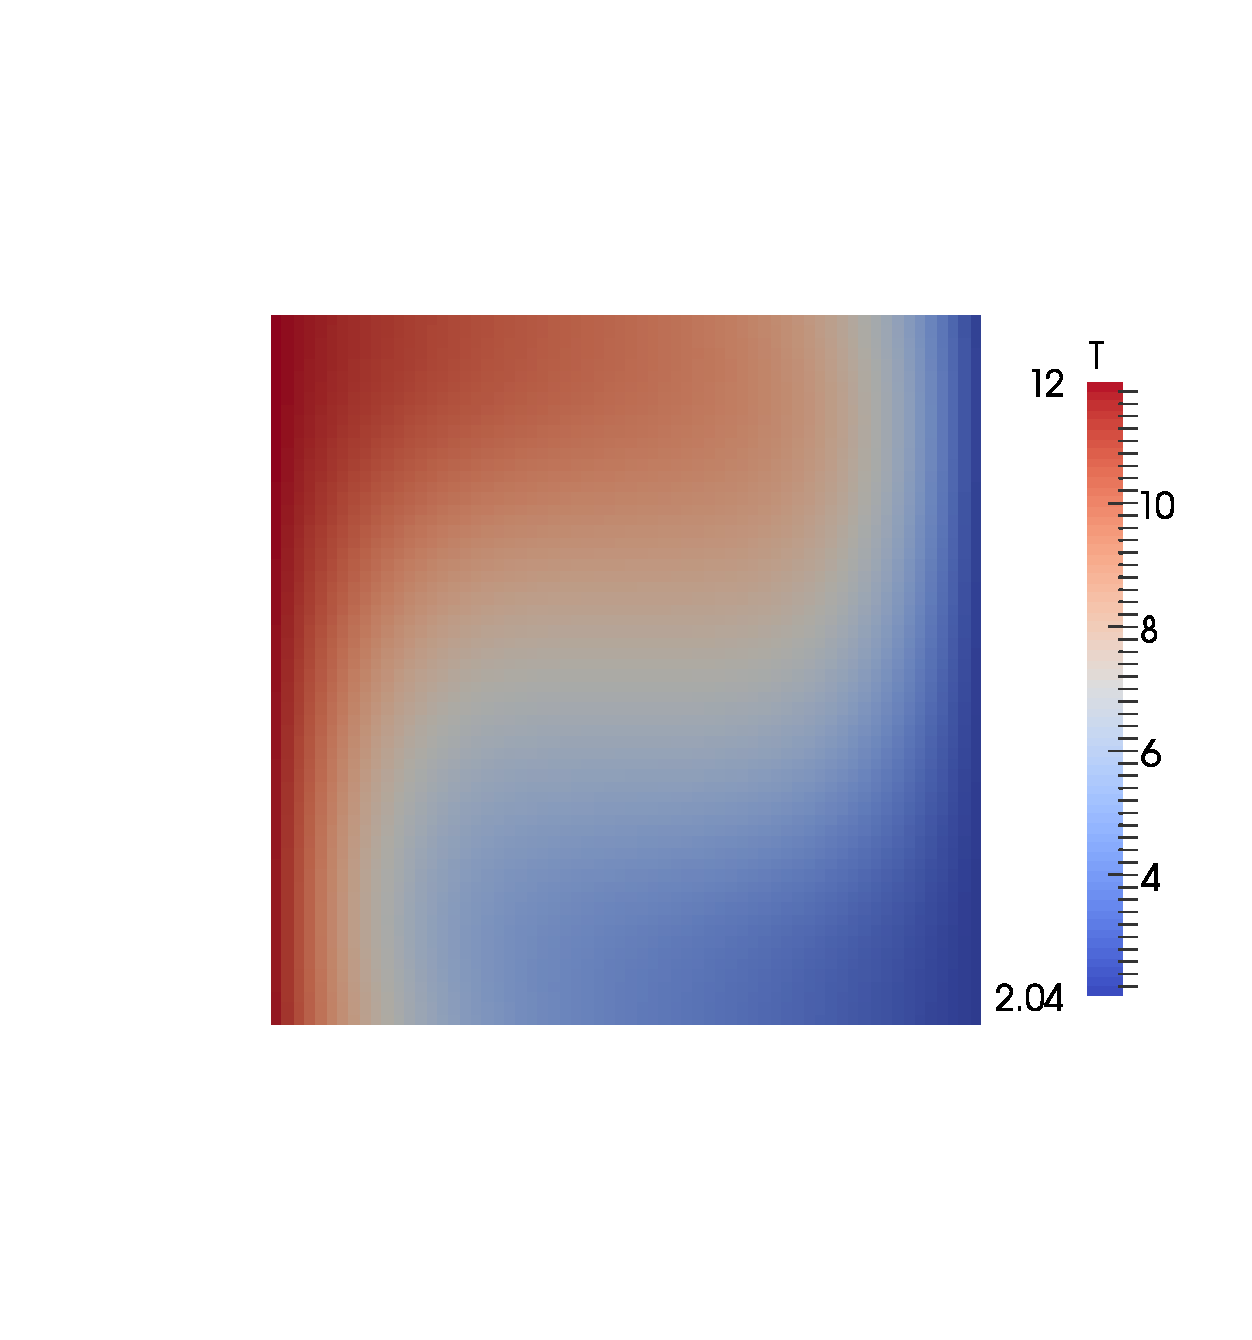
\includegraphics[trim=3.5cm 5cm 0cm 5cm, scale=0.5,clip=true]{./img/cavity.pdf}
  \raggedleft{}
\end{minipage}}
\hfil
\subfigure{
\begin{minipage}{0.45\textwidth}
  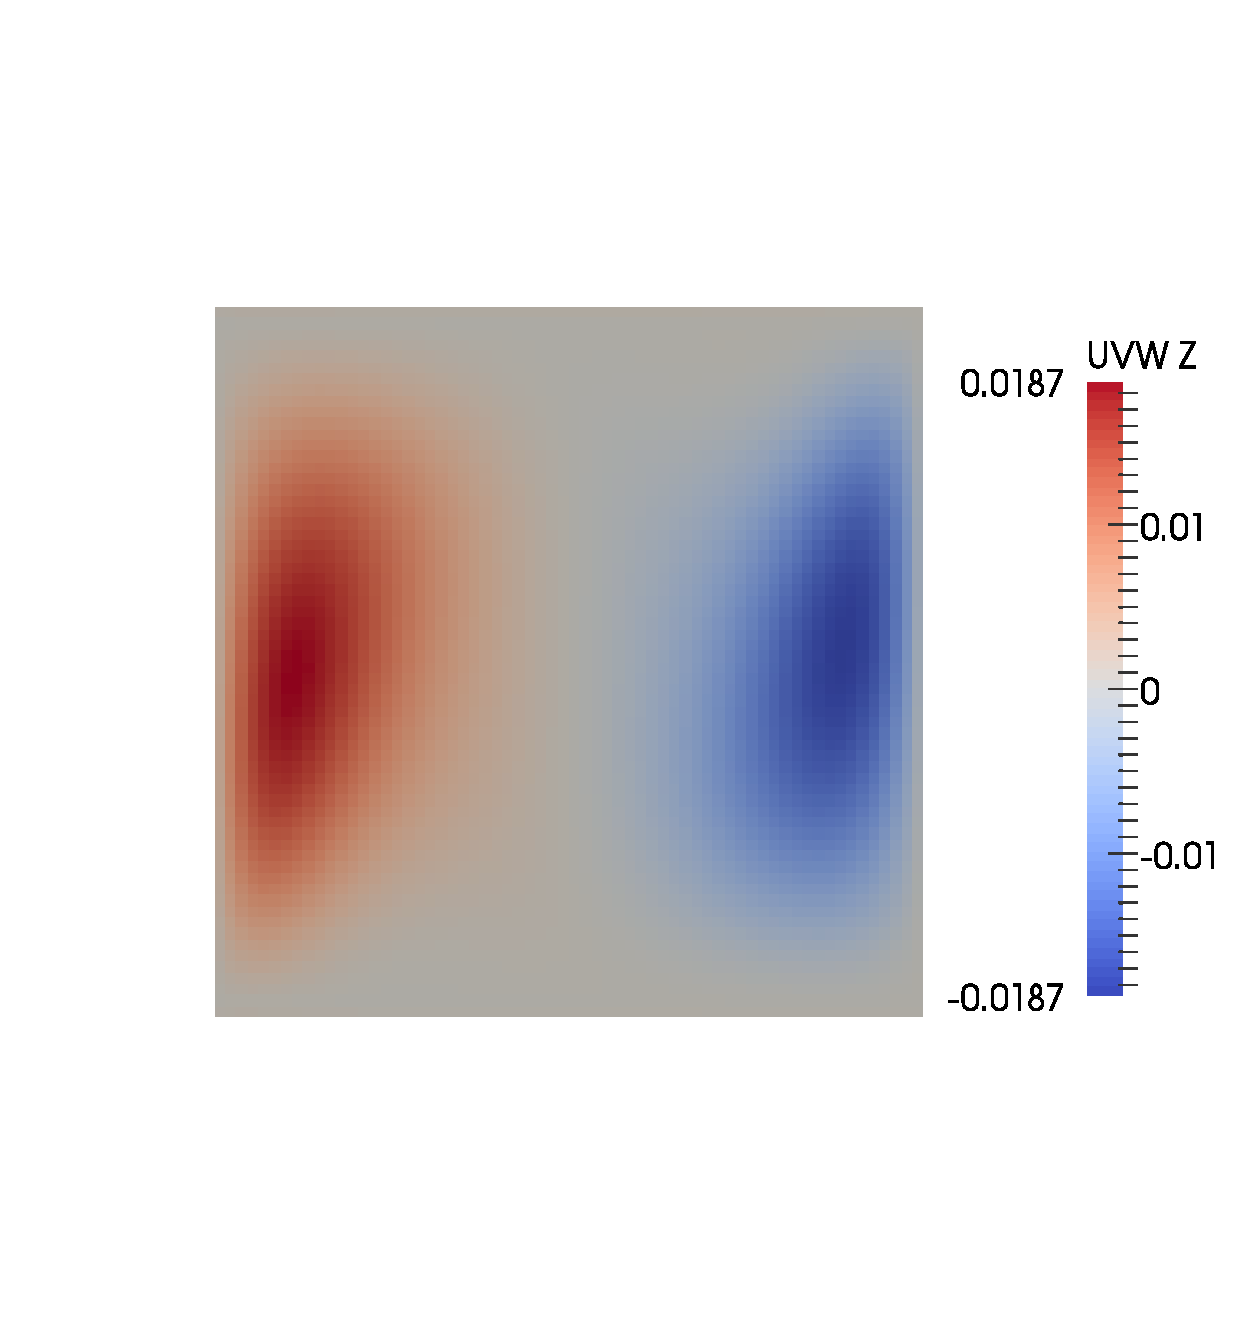
\includegraphics[trim=3.5cm 4.5cm 0cm 5cm, scale=0.5,clip=true]{./img/cavityw.pdf}
\end{minipage} }
  \caption{Temperature field and velocity field in the coordinate direction of the gravitational force of the temperature-driven cavity flow problem for a cross section in the middle of the problem domain }
  \label{fig:sketchcavity}
\end{figure}

Essential for this benchmarking case is the nature of the flow. The fluid motion is a consequence of the effect of volume forces caused by temperature differences in the solution domain, hence the mathematical problem exhibits a strong coupling between the involved variables velocity, pressure and temperature. This relation is represented by the Rayleigh and Prandtl number. It is assumed that for this kind of flow the fully implicit treatment of the temperature coupling will yield further benefits with respect to wall-clock time, compared with solution approaches that solve for the temperature separately. Table \ref{tab:cavity} lists the geometrical and solver parameters used for the performance analysis of this section.

\begin{table}[h!]\centering
  \caption{Characteristic problem properties used in the heated cavity flow test case}
\ra{1.3}
  \begin{tabular}{lcc}\toprule
    Property & Value & Unit \\
    \midrule
    \rowcolor{black!20} Density            & 1.19      & $kg/m^3$  \\
    \rowcolor{black!00} Viscosity          & 1.8E-5    & $Ns/m^2$  \\
    \rowcolor{black!20} Height             & 0.021277  & m         \\
    \rowcolor{black!00} Temperature difference & 10    & K         \\
    \rowcolor{black!20} Coefficient of thermal expansion & 0.00341 & $1/K$ \\
    \rowcolor{black!00} Under-relaxation u & 0.8       &           \\
    \rowcolor{black!20} Under-relaxation p & 0.2       &           \\
    \rowcolor{black!00} Under-relaxation T & 1.0       &           \\
    \rowcolor{black!20} Relative tolerance & 1E-8      &
  \end{tabular}
  \label{tab:cavity}
\end{table}

Using the data from table \ref{tab:cavity} and given a Prandtl number for the flow problem \(Pr = 0.71\), the Rayleigh number \(Ra\), a dimensionless number used to characterize buoyancy driven flows, can be calculated. From the definition of the Prandtl number, the thermal diffusivity \(\alpha\) can be calculated as
\begin{displaymath}
  \alpha = \frac{\mu}{\rho \, Pr} = 2.1304 * 10^{-5}.
\end{displaymath}
It follows, that the Rayleigh number can be determined to 
\begin{displaymath}
  Ra = \frac{\rho g \beta \Delta T h^3}{\mu \alpha} \approx 10^4,
\end{displaymath}
which implies, according to \cite{christon02}, that the flow is still stationary and non-turbulent.

The tests were conducted on the formerly presented HHLR cluster, using the MPI2 section. Table \ref{tab:cavitycompare} compares the wall-clock times and numbers of needed outer iterations for different solver and coupling approaches. The presented results are in good agreement with \cite{vakilipour12}, which show monotonic decrease of the number of iterations with increased implicit coupling for a different test case. It is notable, that the pressure velocity coupling is responsible for the biggest decrease in the number of non-linear iterations. Different to the results presented in section \ref{sec:channel}, this does not yield significant performance benefits with respect to wall-clock time. In order to achieve the benefits of a fully coupled solution algorithm, the coupling has to be increased to also involve semi-implicit temperature-to-velocity/pressure and implicit velocity-to-temperature coupling. In this context the abbreviations \emph{SEG} for the segregated solution algorithm and \emph{CPLD} for the fully coupled solution algorithm without implicit temperature coupling are used. For the fully coupled solver configurations, \emph{TCPLD} includes only implicit velocity-to-temperature coupling, whereas \emph{NRCPLD} additionally includes implicit temperature-to-velocity/pressure coupling via the Newton-Raphson linearization.

\begin{table}[h!]\centering
\ra{1.3}
  \caption{Performance analysis results of the temperature-driven cavity flow problem comparing the SIMPLE-algorithm with segregated temperature solve (SEG), the fully coupled solution algorithm with segregated temperature solve (CPLD), the fully coupled solution algorithm with an implicit Boussinesq approximation (TCPLD) and the fully coupled solution algorithm using an implicit Boussinesq approximation and a semi-implicit Newton-Raphson linearization of the convective part of the temperature equation (NRCPLD).}
  \begin{tabular}{cccc}\toprule
    Resolution & Solver configuration & Time s & No. Non-linear its. \\
    \midrule
    \rowcolor{black!20}\multirow{4}{*}{}            & SEG    & 0.3719E+02 & 203 \\
    \rowcolor{black!20}                             & CPLD   & 0.6861E+02 & 62  \\
    \rowcolor{black!20}                             & TCPLD  & 0.1012E+03 & 31  \\
    \rowcolor{black!20} \multirow{-4}{*}{32x32x32}  & NRCPLD & 0.2153E+02 & 22  \\ %\hline
    %
    \rowcolor{black!00}\multirow{4}{*}{}            & SEG    & 0.1997E+04 &  804 \\
    \rowcolor{black!00}                             & CPLD   & 0.7687E+03 &  63  \\
    \rowcolor{black!00}                             & TCPLD  & 0.1278E+04 &  59  \\
    \rowcolor{black!00} \multirow{-4}{*}{64x64x64}  & NRCPLD & 0.4240E+03 &  17  \\ %\hline
    %
    \rowcolor{black!20}\multirow{4}{*}{}               & SEG    & 0.5197E+05 &  3060 \\
    \rowcolor{black!20}                                & CPLD   & 0.1860E+05 &  74   \\
    \rowcolor{black!20}                                & TCPLD  & 0.1950E+05 &  50   \\
    \rowcolor{black!20} \multirow{-4}{*}{128x128x128}  & NRCPLD & 0.6155E+04 &  18   \\ %\hline
    %
    %\rowcolor{black!00}\multirow{4}{*}{}               & SEG    &  & \\
    %\rowcolor{black!00}                                & CPLD   &  & \\
    %\rowcolor{black!00}                                & TCPLD  &  & \\
    %\rowcolor{black!00} \multirow{-4}{*}{256x256x256}  & NRCPLD &  & \\ %\hline
  \end{tabular}
  \label{tab:cavitycompare}
\end{table}

It can be noticed from table \ref{tab:cavitycompare}, that the solely use of velocity-to-temperature coupling does not result in benefits compared to the coupled solution for velocities and pressure combined with a decoupled solve for the temperature equation. This is accredited to the treatment of the non-linearity of the temperature equation in the TCPLD solver configuration. Even though the momentum balances implicitly use the temperature from the next iteration, the temperature equation does not use the velocities of the next iteration. Instead the convective fluxes are calculated with the velocities from the previous iteration. Even though the implicit velocity-to-temperature coupling reduces the number of needed non-linear iterations an increase in the needed wall-clock time for computation can be noticed. This is attributed to the augmented costs during the application of the linear solver algorithm as a result of the additional degree of freedom that the linear system embraces. The necessary number of outer iterations is higher than in the NRCPLD configuration, since the convective fluxes in the temperature equation are not coupled to the momentum balances, which degrades the convergence of the non-linear iteration process.

It can be concluded, that in order to profit from the benefits of implicit coupling, the key lies in the semi-implicit temperature-to-velocity/pressure coupling. However, it should be noted, that the implicit consideration of the corresponding terms furthermore increases the amount of memory needed for computation and hence does not come without deficiencies.

\subsection{Effect of Different Non-Orthogonal Correctors on Solver Convergence}
\label{sec:studynonorth}

Section \ref{sec:nonorth} introduced different ways to address the degradation of the grid quality due to non-orthogonality of the grid. This section compares the three different correctors, the orthogonal correction, the minimum correction and the over-relaxed approach, which are used in the discretization process of the gradients at cell boundary faces. For this purpose the grid generator program of section \ref{sec:gridpreproc} was extended to generate skewed grids. A random number generator was used to move each inner grid point within a specified neighborhood of the original location and to skew the grid. Figure \ref{fig:nonorthgrid} illustrates the concept for a two-dimensional \(8 \times 8\) grid. It is evident that the previous orthogonality of the grid is lost and the need for non-orthogonal correctors becomes visible. It should be noted that even in the case of orthogonal grids, non-orthogonal correction may become necessary to treat fluxes across block boundaries if neighboring blocks have been locally refined. To maintain the grid's integrity after the movement of the grid points the neighborhoods were limited by half the distance \(\Delta x\) of two neighboring grid points, as indicated for on point in figure \ref{fig:nonorthgrid}.

\begin{figure}[h!]
  \begin{center}
    \begin{tikzpicture}[scale=3.0]

\draw (-1.0000000  ,-1.0000000) --   (-1.0000000  ,-0.7500000) --   (-0.7500000  ,-0.7500000) --   (-0.7500000  ,-1.0000000) -- cycle;
\draw (-1.0000000  ,-0.7500000) --   (-1.0000000  ,-0.5000000) --   (-0.7500000  ,-0.5000000) --   (-0.7500000  ,-0.7500000) -- cycle;
\draw (-1.0000000  ,-0.5000000) --   (-1.0000000  ,-0.2500000) --   (-0.7500000  ,-0.2500000) --   (-0.7500000  ,-0.5000000) -- cycle;
\draw (-1.0000000  ,-0.2500000) --   (-1.0000000  , 0.0000000) --   (-0.7500000  , 0.0000000) --   (-0.7500000  ,-0.2500000) -- cycle;
\draw (-1.0000000  , 0.0000000) --   (-1.0000000  , 0.2500000) --   (-0.7500000  , 0.2500000) --   (-0.7500000  , 0.0000000) -- cycle;
\draw (-1.0000000  , 0.2500000) --   (-1.0000000  , 0.5000000) --   (-0.7500000  , 0.5000000) --   (-0.7500000  , 0.2500000) -- cycle;
\draw (-1.0000000  , 0.5000000) --   (-1.0000000  , 0.7500000) --   (-0.7500000  , 0.7500000) --   (-0.7500000  , 0.5000000) -- cycle;
\draw (-1.0000000  , 0.7500000) --   (-1.0000000  , 1.0000000) --   (-0.7500000  , 1.0000000) --   (-0.7500000  , 0.7500000) -- cycle;
\draw (-0.7500000  ,-1.0000000) --   (-0.7500000  ,-0.7500000) --   (-0.5000000  ,-0.7500000) --   (-0.5000000  ,-1.0000000) -- cycle;
\draw (-0.7500000  ,-0.7500000) --   (-0.7500000  ,-0.5000000) --   (-0.5000000  ,-0.5000000) --   (-0.5000000  ,-0.7500000) -- cycle;
\draw (-0.7500000  ,-0.5000000) --   (-0.7500000  ,-0.2500000) --   (-0.5000000  ,-0.2500000) --   (-0.5000000  ,-0.5000000) -- cycle;
\draw (-0.7500000  ,-0.2500000) --   (-0.7500000  , 0.0000000) --   (-0.5000000  , 0.0000000) --   (-0.5000000  ,-0.2500000) -- cycle;
\draw (-0.7500000  , 0.0000000) --   (-0.7500000  , 0.2500000) --   (-0.5000000  , 0.2500000) --   (-0.5000000  , 0.0000000) -- cycle;
\draw (-0.7500000  , 0.2500000) --   (-0.7500000  , 0.5000000) --   (-0.5000000  , 0.5000000) --   (-0.5000000  , 0.2500000) -- cycle;
\draw (-0.7500000  , 0.5000000) --   (-0.7500000  , 0.7500000) --   (-0.5000000  , 0.7500000) --   (-0.5000000  , 0.5000000) -- cycle;
\draw (-0.7500000  , 0.7500000) --   (-0.7500000  , 1.0000000) --   (-0.5000000  , 1.0000000) --   (-0.5000000  , 0.7500000) -- cycle;
\draw (-0.5000000  ,-1.0000000) --   (-0.5000000  ,-0.7500000) --   (-0.2500000  ,-0.7500000) --   (-0.2500000  ,-1.0000000) -- cycle;
\draw (-0.5000000  ,-0.7500000) --   (-0.5000000  ,-0.5000000) --   (-0.2500000  ,-0.5000000) --   (-0.2500000  ,-0.7500000) -- cycle;
\draw (-0.5000000  ,-0.5000000) --   (-0.5000000  ,-0.2500000) --   (-0.2500000  ,-0.2500000) --   (-0.2500000  ,-0.5000000) -- cycle;
\draw (-0.5000000  ,-0.2500000) --   (-0.5000000  , 0.0000000) --   (-0.2500000  , 0.0000000) --   (-0.2500000  ,-0.2500000) -- cycle;
\draw (-0.5000000  , 0.0000000) --   (-0.5000000  , 0.2500000) --   (-0.2500000  , 0.2500000) --   (-0.2500000  , 0.0000000) -- cycle;
\draw (-0.5000000  , 0.2500000) --   (-0.5000000  , 0.5000000) --   (-0.2500000  , 0.5000000) --   (-0.2500000  , 0.2500000) -- cycle;
\draw (-0.5000000  , 0.5000000) --   (-0.5000000  , 0.7500000) --   (-0.2500000  , 0.7500000) --   (-0.2500000  , 0.5000000) -- cycle;
\draw (-0.5000000  , 0.7500000) --   (-0.5000000  , 1.0000000) --   (-0.2500000  , 1.0000000) --   (-0.2500000  , 0.7500000) -- cycle;
\draw (-0.2500000  ,-1.0000000) --   (-0.2500000  ,-0.7500000) --   ( 0.0000000  ,-0.7500000) --   ( 0.0000000  ,-1.0000000) -- cycle;
\draw (-0.2500000  ,-0.7500000) --   (-0.2500000  ,-0.5000000) --   ( 0.0000000  ,-0.5000000) --   ( 0.0000000  ,-0.7500000) -- cycle;
\draw (-0.2500000  ,-0.5000000) --   (-0.2500000  ,-0.2500000) --   ( 0.0000000  ,-0.2500000) --   ( 0.0000000  ,-0.5000000) -- cycle;
\draw (-0.2500000  ,-0.2500000) --   (-0.2500000  , 0.0000000) --   ( 0.0000000  , 0.0000000) --   ( 0.0000000  ,-0.2500000) -- cycle;
\draw (-0.2500000  , 0.0000000) --   (-0.2500000  , 0.2500000) --   ( 0.0000000  , 0.2500000) --   ( 0.0000000  , 0.0000000) -- cycle;
\draw (-0.2500000  , 0.2500000) --   (-0.2500000  , 0.5000000) --   ( 0.0000000  , 0.5000000) --   ( 0.0000000  , 0.2500000) -- cycle;
\draw (-0.2500000  , 0.5000000) --   (-0.2500000  , 0.7500000) --   ( 0.0000000  , 0.7500000) --   ( 0.0000000  , 0.5000000) -- cycle;
\draw (-0.2500000  , 0.7500000) --   (-0.2500000  , 1.0000000) --   ( 0.0000000  , 1.0000000) --   ( 0.0000000  , 0.7500000) -- cycle;
\draw ( 0.0000000  ,-1.0000000) --   ( 0.0000000  ,-0.7500000) --   ( 0.2500000  ,-0.7500000) --   ( 0.2500000  ,-1.0000000) -- cycle;
\draw ( 0.0000000  ,-0.7500000) --   ( 0.0000000  ,-0.5000000) --   ( 0.2500000  ,-0.5000000) --   ( 0.2500000  ,-0.7500000) -- cycle;
\draw ( 0.0000000  ,-0.5000000) --   ( 0.0000000  ,-0.2500000) --   ( 0.2500000  ,-0.2500000) --   ( 0.2500000  ,-0.5000000) -- cycle;
\draw ( 0.0000000  ,-0.2500000) --   ( 0.0000000  , 0.0000000) --   ( 0.2500000  , 0.0000000) --   ( 0.2500000  ,-0.2500000) -- cycle;
\draw ( 0.0000000  , 0.0000000) --   ( 0.0000000  , 0.2500000) --   ( 0.2500000  , 0.2500000) --   ( 0.2500000  , 0.0000000) -- cycle;
\draw ( 0.0000000  , 0.2500000) --   ( 0.0000000  , 0.5000000) --   ( 0.2500000  , 0.5000000) --   ( 0.2500000  , 0.2500000) -- cycle;
\draw ( 0.0000000  , 0.5000000) --   ( 0.0000000  , 0.7500000) --   ( 0.2500000  , 0.7500000) --   ( 0.2500000  , 0.5000000) -- cycle;
\draw ( 0.0000000  , 0.7500000) --   ( 0.0000000  , 1.0000000) --   ( 0.2500000  , 1.0000000) --   ( 0.2500000  , 0.7500000) -- cycle;
\draw ( 0.2500000  ,-1.0000000) --   ( 0.2500000  ,-0.7500000) --   ( 0.5000000  ,-0.7500000) --   ( 0.5000000  ,-1.0000000) -- cycle;
\draw ( 0.2500000  ,-0.7500000) --   ( 0.2500000  ,-0.5000000) --   ( 0.5000000  ,-0.5000000) --   ( 0.5000000  ,-0.7500000) -- cycle;
\draw ( 0.2500000  ,-0.5000000) --   ( 0.2500000  ,-0.2500000) --   ( 0.5000000  ,-0.2500000) --   ( 0.5000000  ,-0.5000000) -- cycle;
\draw ( 0.2500000  ,-0.2500000) --   ( 0.2500000  , 0.0000000) --   ( 0.5000000  , 0.0000000) --   ( 0.5000000  ,-0.2500000) -- cycle;
\draw ( 0.2500000  , 0.0000000) --   ( 0.2500000  , 0.2500000) --   ( 0.5000000  , 0.2500000) --   ( 0.5000000  , 0.0000000) -- cycle;
\draw ( 0.2500000  , 0.2500000) --   ( 0.2500000  , 0.5000000) --   ( 0.5000000  , 0.5000000) --   ( 0.5000000  , 0.2500000) -- cycle;
\draw ( 0.2500000  , 0.5000000) --   ( 0.2500000  , 0.7500000) --   ( 0.5000000  , 0.7500000) --   ( 0.5000000  , 0.5000000) -- cycle;
\draw ( 0.2500000  , 0.7500000) --   ( 0.2500000  , 1.0000000) --   ( 0.5000000  , 1.0000000) --   ( 0.5000000  , 0.7500000) -- cycle;
\draw ( 0.5000000  ,-1.0000000) --   ( 0.5000000  ,-0.7500000) --   ( 0.7500000  ,-0.7500000) --   ( 0.7500000  ,-1.0000000) -- cycle;
\draw ( 0.5000000  ,-0.7500000) --   ( 0.5000000  ,-0.5000000) --   ( 0.7500000  ,-0.5000000) --   ( 0.7500000  ,-0.7500000) -- cycle;
\draw ( 0.5000000  ,-0.5000000) --   ( 0.5000000  ,-0.2500000) --   ( 0.7500000  ,-0.2500000) --   ( 0.7500000  ,-0.5000000) -- cycle;
\draw ( 0.5000000  ,-0.2500000) --   ( 0.5000000  , 0.0000000) --   ( 0.7500000  , 0.0000000) --   ( 0.7500000  ,-0.2500000) -- cycle;
\draw ( 0.5000000  , 0.0000000) --   ( 0.5000000  , 0.2500000) --   ( 0.7500000  , 0.2500000) --   ( 0.7500000  , 0.0000000) -- cycle;
\draw ( 0.5000000  , 0.2500000) --   ( 0.5000000  , 0.5000000) --   ( 0.7500000  , 0.5000000) --   ( 0.7500000  , 0.2500000) -- cycle;
\draw ( 0.5000000  , 0.5000000) --   ( 0.5000000  , 0.7500000) --   ( 0.7500000  , 0.7500000) --   ( 0.7500000  , 0.5000000) -- cycle;
\draw ( 0.5000000  , 0.7500000) --   ( 0.5000000  , 1.0000000) --   ( 0.7500000  , 1.0000000) --   ( 0.7500000  , 0.7500000) -- cycle;
\draw ( 0.7500000  ,-1.0000000) --   ( 0.7500000  ,-0.7500000) --   ( 1.0000000  ,-0.7500000) --   ( 1.0000000  ,-1.0000000) -- cycle;
\draw ( 0.7500000  ,-0.7500000) --   ( 0.7500000  ,-0.5000000) --   ( 1.0000000  ,-0.5000000) --   ( 1.0000000  ,-0.7500000) -- cycle;
\draw ( 0.7500000  ,-0.5000000) --   ( 0.7500000  ,-0.2500000) --   ( 1.0000000  ,-0.2500000) --   ( 1.0000000  ,-0.5000000) -- cycle;
\draw ( 0.7500000  ,-0.2500000) --   ( 0.7500000  , 0.0000000) --   ( 1.0000000  , 0.0000000) --   ( 1.0000000  ,-0.2500000) -- cycle;
\draw ( 0.7500000  , 0.0000000) --   ( 0.7500000  , 0.2500000) --   ( 1.0000000  , 0.2500000) --   ( 1.0000000  , 0.0000000) -- cycle;
\draw ( 0.7500000  , 0.2500000) --   ( 0.7500000  , 0.5000000) --   ( 1.0000000  , 0.5000000) --   ( 1.0000000  , 0.2500000) -- cycle;
\draw ( 0.7500000  , 0.5000000) --   ( 0.7500000  , 0.7500000) --   ( 1.0000000  , 0.7500000) --   ( 1.0000000  , 0.5000000) -- cycle;
\draw ( 0.7500000  , 0.7500000) --   ( 0.7500000  , 1.0000000) --   ( 1.0000000  , 1.0000000) --   ( 1.0000000  , 0.7500000) -- cycle;

\begin{scope}[shift={(3,0)}]

\draw (-1.0000000  ,-1.0000000) --   (-1.0000000  ,-0.7500000) --   (-0.7357947  ,-0.7251621) --   (-0.7500000  ,-1.0000000) -- cycle;
\draw (-1.0000000  ,-0.7500000) --   (-1.0000000  ,-0.5000000) --   (-0.7931504  ,-0.4600445) --   (-0.7357947  ,-0.7251621) -- cycle;
\draw (-1.0000000  ,-0.5000000) --   (-1.0000000  ,-0.2500000) --   (-0.7525730  ,-0.3061433) --   (-0.7931504  ,-0.4600445) -- cycle;
\draw (-1.0000000  ,-0.2500000) --   (-1.0000000  , 0.0000000) --   (-0.7449333  , 0.0075492) --   (-0.7525730  ,-0.3061433) -- cycle;
\draw (-1.0000000  , 0.0000000) --   (-1.0000000  , 0.2500000) --   (-0.7484480  , 0.2665454) --   (-0.7449333  , 0.0075492) -- cycle;
\draw (-1.0000000  , 0.2500000) --   (-1.0000000  , 0.5000000) --   (-0.6912805  , 0.5417040) --   (-0.7484480  , 0.2665454) -- cycle;
\draw (-1.0000000  , 0.5000000) --   (-1.0000000  , 0.7500000) --   (-0.7723776  , 0.7611020) --   (-0.6912805  , 0.5417040) -- cycle;
\draw (-1.0000000  , 0.7500000) --   (-1.0000000  , 1.0000000) --   (-0.7500000  , 1.0000000) --   (-0.7723776  , 0.7611020) -- cycle;
\draw (-0.7500000  ,-1.0000000) --   (-0.7357947  ,-0.7251621) --   (-0.4595279  ,-0.7841521) --   (-0.5000000  ,-1.0000000) -- cycle;
\draw (-0.7357947  ,-0.7251621) --   (-0.7931504  ,-0.4600445) --   (-0.5311806  ,-0.5308476) --   (-0.4595279  ,-0.7841521) -- cycle;
\draw (-0.7931504  ,-0.4600445) --   (-0.7525730  ,-0.3061433) --   (-0.5153706  ,-0.2151799) --   (-0.5311806  ,-0.5308476) -- cycle;
\draw (-0.7525730  ,-0.3061433) --   (-0.7449333  , 0.0075492) --   (-0.4389612  ,-0.0466777) --   (-0.5153706  ,-0.2151799) -- cycle;
\draw (-0.7449333  , 0.0075492) --   (-0.7484480  , 0.2665454) --   (-0.5252782  , 0.2740304) --   (-0.4389612  ,-0.0466777) -- cycle;
\draw (-0.7484480  , 0.2665454) --   (-0.6912805  , 0.5417040) --   (-0.4807991  , 0.5242957) --   (-0.5252782  , 0.2740304) -- cycle;
\draw (-0.6912805  , 0.5417040) --   (-0.7723776  , 0.7611020) --   (-0.4834101  , 0.7570882) --   (-0.4807991  , 0.5242957) -- cycle;
\draw (-0.7723776  , 0.7611020) --   (-0.7500000  , 1.0000000) --   (-0.5000000  , 1.0000000) --   (-0.4834101  , 0.7570882) -- cycle;
\draw (-0.5000000  ,-1.0000000) --   (-0.4595279  ,-0.7841521) --   (-0.2182362  ,-0.6917532) --   (-0.2500000  ,-1.0000000) -- cycle;
\draw (-0.4595279  ,-0.7841521) --   (-0.5311806  ,-0.5308476) --   (-0.2305534  ,-0.4572581) --   (-0.2182362  ,-0.6917532) -- cycle;
\draw (-0.5311806  ,-0.5308476) --   (-0.5153706  ,-0.2151799) --   (-0.2675149  ,-0.2501086) --   (-0.2305534  ,-0.4572581) -- cycle;
\draw (-0.5153706  ,-0.2151799) --   (-0.4389612  ,-0.0466777) --   (-0.2980465  , 0.0160808) --   (-0.2675149  ,-0.2501086) -- cycle;
\draw (-0.4389612  ,-0.0466777) --   (-0.5252782  , 0.2740304) --   (-0.2163867  , 0.2431438) --   (-0.2980465  , 0.0160808) -- cycle;
\draw (-0.5252782  , 0.2740304) --   (-0.4807991  , 0.5242957) --   (-0.2537808  , 0.4964562) --   (-0.2163867  , 0.2431438) -- cycle;
\draw (-0.4807991  , 0.5242957) --   (-0.4834101  , 0.7570882) --   (-0.3105596  , 0.7358472) --   (-0.2537808  , 0.4964562) -- cycle;
\draw (-0.4834101  , 0.7570882) --   (-0.5000000  , 1.0000000) --   (-0.2500000  , 1.0000000) --   (-0.3105596  , 0.7358472) -- cycle;
\draw (-0.2500000  ,-1.0000000) --   (-0.2182362  ,-0.6917532) --   (-0.0482077  ,-0.7551043) --   ( 0.0000000  ,-1.0000000) -- cycle;
\draw (-0.2182362  ,-0.6917532) --   (-0.2305534  ,-0.4572581) --   ( 0.0008446  ,-0.4652540) --   (-0.0482077  ,-0.7551043) -- cycle;
\draw (-0.2305534  ,-0.4572581) --   (-0.2675149  ,-0.2501086) --   ( 0.0200666  ,-0.2737875) --   ( 0.0008446  ,-0.4652540) -- cycle;
\draw (-0.2675149  ,-0.2501086) --   (-0.2980465  , 0.0160808) --   ( 0.0552534  ,-0.0126174) --   ( 0.0200666  ,-0.2737875) -- cycle;
\draw (-0.2980465  , 0.0160808) --   (-0.2163867  , 0.2431438) --   ( 0.0011075  , 0.2269005) --   ( 0.0552534  ,-0.0126174) -- cycle;
\draw (-0.2163867  , 0.2431438) --   (-0.2537808  , 0.4964562) --   ( 0.0309617  , 0.5500598) --   ( 0.0011075  , 0.2269005) -- cycle;
\draw (-0.2537808  , 0.4964562) --   (-0.3105596  , 0.7358472) --   (-0.0513426  , 0.7758411) --   ( 0.0309617  , 0.5500598) -- cycle;
\draw (-0.3105596  , 0.7358472) --   (-0.2500000  , 1.0000000) --   ( 0.0000000  , 1.0000000) --   (-0.0513426  , 0.7758411) -- cycle;
\draw ( 0.0000000  ,-1.0000000) --   (-0.0482077  ,-0.7551043) --   ( 0.2471987  ,-0.7582445) --   ( 0.2500000  ,-1.0000000) -- cycle;
\draw (-0.0482077  ,-0.7551043) --   ( 0.0008446  ,-0.4652540) --   ( 0.1963613  ,-0.4770231) --   ( 0.2471987  ,-0.7582445) -- cycle;
\draw ( 0.0008446  ,-0.4652540) --   ( 0.0200666  ,-0.2737875) --   ( 0.2961292  ,-0.2302816) --   ( 0.1963613  ,-0.4770231) -- cycle;
\draw ( 0.0200666  ,-0.2737875) --   ( 0.0552534  ,-0.0126174) --   ( 0.2068714  ,-0.0503173) --   ( 0.2961292  ,-0.2302816) -- cycle;
\draw ( 0.0552534  ,-0.0126174) --   ( 0.0011075  , 0.2269005) --   ( 0.3050563  , 0.1893252) --   ( 0.2068714  ,-0.0503173) -- cycle;
\draw ( 0.0011075  , 0.2269005) --   ( 0.0309617  , 0.5500598) --   ( 0.2263998  , 0.4997990) --   ( 0.3050563  , 0.1893252) -- cycle;
\draw ( 0.0309617  , 0.5500598) --   (-0.0513426  , 0.7758411) --   ( 0.2751040  , 0.6906821) --   ( 0.2263998  , 0.4997990) -- cycle;
\draw (-0.0513426  , 0.7758411) --   ( 0.0000000  , 1.0000000) --   ( 0.2500000  , 1.0000000) --   ( 0.2751040  , 0.6906821) -- cycle;
\draw ( 0.2500000  ,-1.0000000) --   ( 0.2471987  ,-0.7582445) --   ( 0.5382664  ,-0.6978459) --   ( 0.5000000  ,-1.0000000) -- cycle;
\draw ( 0.2471987  ,-0.7582445) --   ( 0.1963613  ,-0.4770231) --   ( 0.5126137  ,-0.4590502) --   ( 0.5382664  ,-0.6978459) -- cycle;
\draw ( 0.1963613  ,-0.4770231) --   ( 0.2961292  ,-0.2302816) --   ( 0.4815557  ,-0.2873007) --   ( 0.5126137  ,-0.4590502) -- cycle;
\draw ( 0.2961292  ,-0.2302816) --   ( 0.2068714  ,-0.0503173) --   ( 0.4740993  , 0.0532870) --   ( 0.4815557  ,-0.2873007) -- cycle;
\draw ( 0.2068714  ,-0.0503173) --   ( 0.3050563  , 0.1893252) --   ( 0.4967194  , 0.2012874) --   ( 0.4740993  , 0.0532870) -- cycle;
\draw ( 0.3050563  , 0.1893252) --   ( 0.2263998  , 0.4997990) --   ( 0.4603611  , 0.4728257) --   ( 0.4967194  , 0.2012874) -- cycle;
\draw ( 0.2263998  , 0.4997990) --   ( 0.2751040  , 0.6906821) --   ( 0.4672861  , 0.7466205) --   ( 0.4603611  , 0.4728257) -- cycle;
\draw ( 0.2751040  , 0.6906821) --   ( 0.2500000  , 1.0000000) --   ( 0.5000000  , 1.0000000) --   ( 0.4672861  , 0.7466205) -- cycle;
\draw ( 0.5000000  ,-1.0000000) --   ( 0.5382664  ,-0.6978459) --   ( 0.7078082  ,-0.7837875) --   ( 0.7500000  ,-1.0000000) -- cycle;
\draw ( 0.5382664  ,-0.6978459) --   ( 0.5126137  ,-0.4590502) --   ( 0.7276430  ,-0.4948496) --   ( 0.7078082  ,-0.7837875) -- cycle;
\draw ( 0.5126137  ,-0.4590502) --   ( 0.4815557  ,-0.2873007) --   ( 0.6920666  ,-0.2745631) --   ( 0.7276430  ,-0.4948496) -- cycle;
\draw ( 0.4815557  ,-0.2873007) --   ( 0.4740993  , 0.0532870) --   ( 0.7981546  ,-0.0118967) --   ( 0.6920666  ,-0.2745631) -- cycle;
\draw ( 0.4740993  , 0.0532870) --   ( 0.4967194  , 0.2012874) --   ( 0.6919272  , 0.3090704) --   ( 0.7981546  ,-0.0118967) -- cycle;
\draw ( 0.4967194  , 0.2012874) --   ( 0.4603611  , 0.4728257) --   ( 0.7440529  , 0.5171666) --   ( 0.6919272  , 0.3090704) -- cycle;
\draw ( 0.4603611  , 0.4728257) --   ( 0.4672861  , 0.7466205) --   ( 0.8019544  , 0.7630775) --   ( 0.7440529  , 0.5171666) -- cycle;
\draw ( 0.4672861  , 0.7466205) --   ( 0.5000000  , 1.0000000) --   ( 0.7500000  , 1.0000000) --   ( 0.8019544  , 0.7630775) -- cycle;
\draw ( 0.7500000  ,-1.0000000) --   ( 0.7078082  ,-0.7837875) --   ( 1.0000000  ,-0.7500000) --   ( 1.0000000  ,-1.0000000) -- cycle;
\draw ( 0.7078082  ,-0.7837875) --   ( 0.7276430  ,-0.4948496) --   ( 1.0000000  ,-0.5000000) --   ( 1.0000000  ,-0.7500000) -- cycle;
\draw ( 0.7276430  ,-0.4948496) --   ( 0.6920666  ,-0.2745631) --   ( 1.0000000  ,-0.2500000) --   ( 1.0000000  ,-0.5000000) -- cycle;
\draw ( 0.6920666  ,-0.2745631) --   ( 0.7981546  ,-0.0118967) --   ( 1.0000000  , 0.0000000) --   ( 1.0000000  ,-0.2500000) -- cycle;
\draw ( 0.7981546  ,-0.0118967) --   ( 0.6919272  , 0.3090704) --   ( 1.0000000  , 0.2500000) --   ( 1.0000000  , 0.0000000) -- cycle;
\draw ( 0.6919272  , 0.3090704) --   ( 0.7440529  , 0.5171666) --   ( 1.0000000  , 0.5000000) --   ( 1.0000000  , 0.2500000) -- cycle;
\draw ( 0.7440529  , 0.5171666) --   ( 0.8019544  , 0.7630775) --   ( 1.0000000  , 0.7500000) --   ( 1.0000000  , 0.5000000) -- cycle;
\draw ( 0.8019544  , 0.7630775) --   ( 0.7500000  , 1.0000000) --   ( 1.0000000  , 1.0000000) --   ( 1.0000000  , 0.7500000) -- cycle;

\draw (0,0) circle (0.125);
\draw[fill=black] (0,0) circle (0.02);
\draw[fill=black] ( 0.0552534  ,-0.0126174) circle (0.02);

\end{scope}

\draw[->,very thick] (1.1,0) -- (1.9,0) node [midway,below,xshift=0pt,text width=3cm,align=center] {\small random translation \\ of inner points};
\draw (0,0) circle (0.125);
\draw[fill=black] (0,0) circle (0.02);

\end{tikzpicture}

    \caption{Skewing of an initially equidistant, structured and orthogonal grid via random movement of inner grid points within a small neighborhood of their original location. The neighborhood with maximal diameter is indicated by a circle around one inner grid point}
    \label{fig:nonorthgrid}
  \end{center}
\end{figure}

To measure the effect of different non-orthogonal corrections on the solution process, tests for different skewed grids were performed, measuring the number of needed outer iterations to solve for the analytic solution presented in section \ref{sec:manufacturedsolution}.  For this, all correctors addressing grid non-orthogonality from section \ref{sec:nonorth} have been implemented in the coupled solver program. The grid skewness was parametrized with the relative diameter \(\alpha\) of the maximal neighborhood, which constrains the movement of grid points. \(\alpha \in [0,1) \), where \(\alpha = 0\) corresponds to no movement of grid points at all and \(\alpha = 1\) would move grid points up to \(\textstyle \frac{\Delta x}{2} \) away from their original location. The choice of \(\alpha = 1\) is not permitted to maintain the grid's integrity. Such a choice would permit the grid generator to place two grid points at the same location. The calculations were terminated after a reduction of \(10^{-14}\) of the relative initial residual was obtained.

\begin{figure}
  \begin{center}
  \begin{tikzpicture}
    \begin{axis}[
      ylabel={Number of needed outer iterations},
      xlabel={Relative diameter of the neighborhood},
      xtick={0,0.1,0.2,0.3,0.4,0.5,0.6,0.7,0.8,0.9,1.0},
      xmin=0,xmax=1,
      legend pos=outer north east,
      ]
      \addplot[color=black,mark=*]         file {./files/nonorth.mc};
      \addplot[color=black,mark=square*]   file {./files/nonorth.oc};
      \addplot[color=black,mark=triangle*] file {./files/nonorth.or};
      \addlegendentry{Minimum correction};
      \addlegendentry{Orthogonal correction};
      \addlegendentry{Over-relaxed approach};
      \end{axis}
    \end{tikzpicture}
  \end{center}
\caption{Number of needed outer iterations for different relative diameters of the neighborhood in which the movement of grid points takes place, parametrized by the orthogonal corrector}
\label{fig:nonorth}
\end{figure}

The results presented in figure \ref{fig:nonorth} affirm the results presented in \cite{jasak96}. Is can be observed, that for small movements of grid points the choice of corrector does not affect convergence. However as movements of grid points increase, and thus higher non-orthogonality increases, the over-relaxed approach outperforms the other correctors with respect to the number of needed outer iterations. This does directly translate into performance with respect to wall-clock time, since the computational effort of the application of each non-orthogonal corrector is approximately the same.

\subsection{Achieving Ideal Load Balancing by Automatic Matrix Partitioning}

Motivate this special load balancing by giving a pie chart about where the time was spent
Three approaches: Data Partitioning -> scatter data across lots of blocks (pro and cons), matrix does not depend on blocks, complete data partitioning
Formula for Partitioning
Matrix partitioning before and after

